\documentclass[12pt,a4paper]{book}
\setlength{\headheight}{14.5pt} % Fix fancyhdr headheight warning
\setcounter{secnumdepth}{3} 
\usepackage{etoc} 
\usepackage[english]{babel}
% (Remove this line entirely; tcolorbox will be loaded later with options)
\usepackage{tocloft} 
\usepackage{xcolor}
\usepackage{url}
\usepackage{amsmath,amssymb}
\usepackage{rotating}  % 用于横向表格
\usepackage{float}  
\usepackage{enumitem}
\usepackage{chngcntr}
\usepackage{titlesec}
\usepackage{pifont}
\counterwithin{footnote}{chapter}
\usepackage{tikz}
\definecolor{FinanceBlue}{cmyk}{1,0.65,0,0.35}
\usetikzlibrary{calc,positioning,arrows.meta}
\usetikzlibrary{shapes.arrows,shapes.geometric}
\usetikzlibrary{decorations.pathreplacing}
\usetikzlibrary{intersections}
\usepackage{pdflscape}
\usepackage{pgfplots}
\pgfplotsset{compat=1.18} 
%\usepackage[backend=bibtex]{biblatex}
%\addbibresource{defiarticle.bib}
\usepackage{cite}
\usepackage{tabularx}
\usepackage{booktabs}
\usepackage{array}
\usepackage{ragged2e,makecell}
\newcolumntype{Y}{>{\raggedright\arraybackslash
  \hyphenpenalty=10000
  \exhyphenpenalty=10000}X}
\AtBeginEnvironment{tabularx}{\hyphenpenalty=10000\exhyphenpenalty=10000\emergencystretch=2em}
\AtBeginEnvironment{tabular}{\hyphenpenalty=10000\exhyphenpenalty=10000\emergencystretch=2em}

\newcommand{\CaseLabel}[1]{%
  \par\noindent{\color{FinanceBlue}\small\bfseries [#1]}\par\vspace{3pt}%
}
\usepackage{graphicx}
\usepackage{siunitx}
\sisetup{
  table-number-alignment = center, % 数字整体居中
  table-format = 3.2,              % 整数最多3位，小数2位
  table-column-width = 2cm         % 列宽固定为2cm
}
\usepackage{caption}          % 提供 \ContinuedFloat           % [p] 浮动页
%\usepackage[number, sort&compress]{natbib}
\usepackage{hyperref}  
\hypersetup{colorlinks=true,linkcolor=black} 
\usepackage{lipsum} 
\usepackage{etoolbox}
% \usepackage{pifont}          % 提供 \ding 圆圈数字①②③…
\usepackage{microtype}
\usepackage{fancyhdr} % 页眉页脚
\usepackage[most]{tcolorbox}  % 用于定制应用部分的外观
%========================================================
% Opening Case
% Two-color design: FinanceBlue + black
%========================================================

\NewDocumentEnvironment{openingcase}{O{Teaching Illustration}m}{%
  \begin{tcolorbox}[
    enhanced,
    breakable,
    colback=white,
    colframe=white,
    boxrule=0pt,
    sharp corners,
    borderline west={2.2pt}{0pt}{FinanceBlue},
    left=10pt,
    right=8pt,
    top=9pt,
    bottom=9pt,
    before skip=1.2em,
    after skip=1.5em
  ]

  % Opening Case label and case status
  \noindent
  {\color{FinanceBlue}\small\bfseries OPENING CASE\par}
  {\color{FinanceBlue}\scriptsize\bfseries [#1]\par}

  \vspace{3pt}

  % Case title
  \noindent
  {\large\bfseries #2\par}

  \vspace{8pt}

  % Body text
  \setlength{\parindent}{1.5em}
  \setlength{\parskip}{0.3em}
  \noindent
}{%
  \ifstrequal{#1}{Teaching Illustration}{%
    \par\vspace{4pt}
    {\footnotesize\noindent Note: Names, figures, and events in this case are hypothetical and are used solely for pedagogical purposes.\par}%
  }{}%
  \end{tcolorbox}%
}

% \newtcolorbox[auto counter, number within=chapter]{example}[2][]{colback=gray!10!white,colframe=black!80!white,
% fonttitle=\bfseries, title=Example~\thetcbcounter: #2,#1}

\tcbuselibrary{theorems,breakable}

\newtcbtheorem[
  number within=chapter
]{example}{Example}{
  breakable
}{ex}


% \makeatletter
% \renewcommand\thefootnote{(\arabic{footnote})}
% \renewcommand\@makefnmark{%
%   \hbox{\textsuperscript{(\arabic{footnote})}}}
% \makeatother

\makeatletter
\newcommand*\@circlednum[1]{\ding{\numexpr171+#1\relax}}
\renewcommand*\@makefnmark{%
  \hbox{\textsuperscript{\@circlednum{\value{footnote}}}}}
\renewcommand*\thefootnote{\@circlednum{\value{footnote}}}
\makeatother

%========================================================
% Chapter-end modules
%========================================================

% -------------------------------------------------------
% Anchor for an actual chapter-end module
%
% Usage:
%   \TailAnchor{summary}
%   \TailAnchor{keyterms}
% -------------------------------------------------------

\newcommand{\TailAnchor}[1]{%
  \phantomsection
  \hypertarget{sec:\thechapter:#1}{}%
  \label{sec:\thechapter:#1}%
}


% -------------------------------------------------------
% Optional convenience command:
% creates an unnumbered heading and its anchor
%
% Usage:
%   \TailModule{summary}{Summary}
% -------------------------------------------------------

\newcommand{\TailModule}[2]{%
  \TailAnchor{#1}%
  \section*{#2}%
}


% -------------------------------------------------------
% One item in the TOC tail:
% clickable name + page number
% -------------------------------------------------------

\newcommand{\TailLink}[3]{%
  \hyperlink{sec:#1:#2}{#3}\,%
  (\pageref*{sec:#1:#2})%
}


% -------------------------------------------------------
% Names of chapter-end modules
% -------------------------------------------------------

\ExplSyntaxOn

\cs_new:Npn \finance_tail_title:n #1
  {
    \str_case:nnF {#1}
      {

        {summary}      {Summary}
        {mindmap}      {Mind~Map}
        {keyterms}     {Key~Terms}
        {questions}    {Discussion~Questions}
        {appprobs}     {Applied~Problems}
        {aiprompt}     {Financial~AI~Lab}
        {dataapp}      {Data~Application}
        {caseanalysis} {Case~Analysis}
        {furtherread}  {Further~Reading}
      }
      {#1}
  }


% -------------------------------------------------------
% Generates:
%
% Summary (20) · Key Terms (22) · Questions (23)
%
% from:
%
% summary,keyterms,questions
% -------------------------------------------------------

\bool_new:N \l__finance_tail_first_bool

\cs_new_protected:Npn \finance_tail_list:nn #1#2
  {
    \bool_set_true:N \l__finance_tail_first_bool

    \clist_map_inline:nn {#2}
      {
        \bool_if:NF \l__finance_tail_first_bool
          {
            \,\textbullet\,
          }

        \TailLink
          {#1}
          {##1}
          {\finance_tail_title:n {##1}}

        \bool_set_false:N \l__finance_tail_first_bool
      }
  }


\NewDocumentCommand{\HyperTailList}{m m}
  {
    \finance_tail_list:nn {#1}{#2}
  }

\ExplSyntaxOff


% -------------------------------------------------------
% Add one chapter-tail row to the table of contents
%
% Examples:
%
% \ChapterTail{summary,keyterms,questions}
%
% \ChapterTail{summary,mindmap,keyterms,questions,appprobs}
% -------------------------------------------------------

\DeclareRobustCommand{\ChapterTail}[1]{%
  \addtocontents{toc}{%
    \protect\contentsline{section}{%
      \protect\numberline{}%
      \protect\HyperTailList{\thechapter}{#1}%
    }{}{}%
  }%
}


\pagestyle{fancyplain}
\fancyhf{}
\renewcommand{\chaptermark}[1]{\markboth{#1}{}}
\renewcommand{\sectionmark}[1]{\markright{\thesection\ #1}{}}
\fancyhead[LE]{
   % The chapter number only if it's greater than 0 and chapter is defined
   \ifcsname chapter\endcsname
     \ifnum\value{chapter}>0 \chaptername\ \thechapter: \fi
   \fi
   % The chapter title
    \leftmark}  
\fancyhead[CO,RE]{}
\fancyhead[LO,CE]{}
\fancyhead[RO]{\rightmark}
\fancyfoot{}
\fancyfoot[LE,RO]{\thepage}
\fancypagestyle{plain}{
\fancyhead{} % 页眉清空
\renewcommand{\headrulewidth}{0pt} % 去页眉线
\fancyfoot{}
\fancyfoot[LE,RO]{\thepage}
}
\frenchspacing
\setcounter{tocdepth}{4}

\tcbuselibrary{breakable,skins,theorems}
\makeatletter
\newcommand{\applisttitle}[2]{Application~\thetcbcounter: #2}

\newtcolorbox[auto counter,
              number within=chapter,
              list inside=applist]% <— removed list entry key
              {application}[2][]{
  % \newtcolorbox[auto counter, number within=chapter]{application}[2][]{
  enhanced jigsaw,            % 高级皮肤算法
  breakable,                  % 支持分页
  colframe=blue!50!black,     % 边框
  colback=blue!5,             % 背景
  coltitle=black,             % 标题色
  fonttitle=\bfseries,        % 标题加粗
  attach boxed title to top left={xshift=2mm,yshift=-2mm},
  boxed title style={         % 标题盒子样式
    sharp corners,
    colback=blue!20!white,
    colframe=blue!50!black,
    boxrule=0.8pt, size=small,
    left=4pt,right=4pt,top=2pt,bottom=2pt
  },
  title={Application~\thetcbcounter: #2},
  label=#1,
  boxrule=1pt,                % 整体框线粗细
  left=6pt,right=6pt,top=6pt,bottom=6pt,
   before upper={
    \setlength{\parindent}{1.5em}%  ← 后续段落缩进量
    \noindent                               %  ← 取消首段缩进
  },
   overlay first={
     % 底部横线
    \begin{scope}[shift={(frame.south west)}]
      \draw[blue!60!black,line width=0.6pt] (0,0) -- (frame.south east);
    \end{scope}
  },
  % ————— 在“中间段”（跨页）画上下分割线 —————
  overlay middle={
    % 顶部横线
    \begin{scope}[shift={(frame.north west)}]
      \draw[blue!60!black,line width=0.6pt] (0,0) -- (frame.north east);
    \end{scope}
    % 底部横线
    \begin{scope}[shift={(frame.south west)}]
      \draw[blue!60!black,line width=0.6pt] (0,0) -- (frame.south east);
    \end{scope}
  },
   overlay last={
    % 顶部横线
    \begin{scope}[shift={(frame.north west)}]
      \draw[blue!60!black,line width=0.6pt] (0,0) -- (frame.north east);
    \end{scope}
  },
}
\makeatother

% ======= In the preamble =======
\tikzset{
  timeline/.style={-Latex, line width=0.9pt},
  cfup/.style={-Latex, line width=1pt},      % cash inflow (to investor): arrow up
  cfdown/.style={Latex-, line width=1pt},    % cash outflow (from investor): arrow down
  tick/.style={gray, line width=0.5pt}
}
% Helper macro: horizontal axis with year ticks 0..N
\newcommand{\yearaxis}[2]{%
  \draw[timeline] (0,0)--(#1,0);
  \foreach \x in {0,...,#1} {
    \draw[tick] (\x,0.08)--(\x,-0.08);
    \node[below] at (\x,-0.12) {Year \x};
  }
  \node[font=\bfseries] at (#1/2,0.9) {#2};
}


% ------- 3. 正文 -------

\begin{document}
\frontmatter
\title{FINANCIAL MARKETS, INSTITUTIONS, AND INSTRUMENTS: 

An Information, Contract, and Valuation Perspective}
%\subtitle{Some more to know}
\author{Zhang Xiuli}
\date{20-08-2026}
\maketitle  
\pagenumbering{roman}
\newpage

\chapter*{Preface}
\addcontentsline{toc}{chapter}{Preface}

Finance is entering a period in which its visible forms are changing faster than its underlying economic problems. Payments are increasingly digital, trading is increasingly automated, credit decisions draw on new forms of data, financial intermediation is moving across institutions and platforms, and artificial intelligence is lowering the cost of producing and processing information. At the same time, leverage, liquidity, incentives, contractual obligations, and systemic interdependence remain central to financial outcomes. Technological change therefore makes a stable analytical structure more necessary, not less.

This book is organized around one first principle:

\begin{quote}
\textbf{Finance is the economic system through which societies organize exchanges across time and uncertainty. It accomplishes this by generating information, designing and enforcing contracts, and valuing future contingent cash flows. Financial markets, institutions, and instruments are different organizational forms through which these three fundamental functions are implemented.}
\end{quote}

The proposition is a point of departure, not a division of finance into three compartments. Its deeper foundation lies in economics. Resources must be allocated across time; future states are uncertain; individuals differ in preferences, endowments, information, and tolerance for risk; and transactions take place in environments where information is costly, incentives are imperfect, and enforcement is never automatic. If these frictions disappeared, much of the institutional structure of finance would lose its economic purpose. The financial system acquires form because real economies depart from that frictionless benchmark.

Information economics is especially important in understanding this departure. Finance is concerned with promises whose consequences lie in the future, and the parties to those promises rarely possess the same information. Borrowers know more about their projects than lenders, managers know more about firms than outside investors, and insured parties often know more about their behavior and risk than insurers. Screening, signaling, monitoring, disclosure, reputation, collateral, governance, and intermediation arise because information is costly and asymmetrically distributed. They are not peripheral details of financial practice; they help explain why particular markets and institutions exist at all.

Information problems are inseparable from incentives. Once resources have been transferred, behavior may change. A borrower can alter risk, a manager can pursue private benefits, an intermediary can exploit informational advantages, and an investor can withdraw liquidity when doing so is individually rational but collectively destabilizing. Financial arrangements therefore evolve not simply to transmit funds, but to shape behavior under uncertainty. Some of these arrangements take contractual form; others are embedded in governance, market design, institutional reputation, regulation, accounting, clearing, settlement, and the allocation of control rights. Contract is important, but it is one element within a broader economic architecture of incentives and institutions.

This perspective also clarifies the place of valuation. Valuation is not an independent foundation of finance; it is the decision problem that emerges once future benefits, costs, and risks must be compared in the present. Interest rates connect consumption and investment across time. Risk premia compensate for bearing uncertainty. Market prices aggregate information imperfectly and, in turn, influence financing and investment. Valuation therefore sits within the larger economic problem of allocating scarce resources when time, uncertainty, information, and incentives matter.

The organization of this book follows that logic. Part I begins with the foundations of the financial system: intertemporal exchange, uncertainty, money, payments, and liquidity. Part II develops the economic frictions that give financial arrangements their form, with particular attention to information, incentives, intermediation, and valuation. Part III examines the architecture and operation of financial markets, including trading venues, exchange-traded and over-the-counter arrangements, price discovery, clearing, settlement, and market liquidity. Chapter 11 therefore treats derivatives primarily as markets and market infrastructure. Part IV examines the institutions through which financial functions are organized, beginning with commercial banks and extending to investment banks, asset managers, insurers, and shadow banking and digital platforms. Chapter 16 builds on Chapter 12 by examining how credit intermediation, funding, collateral, liquidity transformation, and risk bearing can move beyond traditional bank balance sheets. Part V focuses on the construction, valuation, and risk-management use of financial instruments, including forwards, futures, swaps, options, credit derivatives, and structured claims. It therefore develops the instruments introduced in the market context of Part III rather than repeating that market-structure analysis. Part VI turns to the financial system as a whole, examining systemic risk, central banking, regulation, and policy. Its final chapter revisits the economic frictions introduced in Chapter 1 and the systemic vulnerabilities examined in Chapter 21, using AI, digital money, tokenization, and decentralized finance to test how the organization of finance may change while its underlying economic problems persist.

The method of exposition follows the same hierarchy. Economic mechanisms come first; institutional forms, models, and techniques follow from them. Mathematics is used when it makes a relationship precise. Cases, balance sheets, diagrams, and data are used when they reveal mechanisms that prose alone would obscure. Chinese financial practice is placed within a broader economic framework so that differences in institutions can be understood without mistaking institutional form for economic principle.

Artificial intelligence belongs naturally in this framework because it changes the cost of acquiring, processing, and using information. It may alter screening, research, trading, monitoring, and organizational boundaries. But lower information-processing costs do not remove scarcity, uncertainty, incentives, liquidity constraints, legal enforceability, or systemic externalities. In some settings, faster and more homogeneous decision-making may even strengthen feedback and common exposures. The relevant question is therefore not whether AI transforms finance---it already does---but which economic frictions it reduces, which it leaves intact, and which new forms of dependence it creates.

Finance ultimately concerns the organization of economic life when decisions made today depend on an uncertain future. Its institutions change because technology, law, and markets change; its central problems persist because time, uncertainty, information, incentives, and scarcity persist. A durable study of finance should therefore begin not with the names of institutions or instruments, but with the economic forces that make them necessary and the conditions under which they succeed or fail.

\section*{How to Use This Book}

The chapters use a common set of learning components at the end of the chapter. Their selection depends on the subject matter and learning objectives of each chapter; not every component is required in every chapter. When included, the components follow a consistent order: Summary, Mind Map, Key Terms, Financial AI Lab, Discussion Questions, Applied Problems, Data Application, Case Analysis, and Further Reading. This approach keeps the organization predictable while allowing each chapter to include only those components that add substantive value to its analysis and teaching.

That is the perspective from which this book proceeds.

\cleardoublepage

% \etocrestorecontentsline  
--- 简易目录：只到 chapter ---
\etocsettocdepth{chapter} % 1 = chapter
\renewcommand\contentsname{Short Contents}
\tableofcontents

\cleardoublepage
% --- 详细目录：显示 section（含尾部条目）---
\etocsettocdepth{subsection} % 2 = section, 3 = subsection, etc.
\renewcommand\contentsname{Full Contents}
\tableofcontents
\cleardoublepage

%==== Main Content Area =====
\mainmatter

\part{Foundations of the Financial System}
\chapter{The Essence of Finance: Frictions, Functions, and the Financial System}
\label{chap:The_Essence_of_Finance_Frictions_Functions_and_the_Financial_System}

\begin{openingcase}{A Valuable Project, but No Financing?}

Li Wei, an engineer in Suzhou, has developed an energy-saving control system for industrial equipment. To build a production line and bring the product to market, he needs RMB~10 million today but can invest only RMB~1 million of his own savings.

Elsewhere, Wang Cheng has savings that she does not expect to use in the near future. In a frictionless world, the match would appear obvious: one side has funds, the other has a productive use for them. Yet the exchange does not organize itself.

Wang knows less about the technology than Li. She cannot observe the true quality of the project, verify all of Li's forecasts, or know in advance how he will behave after receiving the funds. The project itself is uncertain. Demand may disappoint, costs may rise, or a competing technology may emerge. Their preferred horizons also differ. Li needs patient financing; Wang may want access to her savings much sooner.

Even if Wang is willing to provide the remaining RMB~9 million, further questions remain. How should the risk be allocated? What information should Li disclose? What rights should Wang receive? How can either side be confident that future obligations will be honored? And if the project is expected to generate cash flows over many years, how much are those uncertain future cash flows worth today?

The availability of savings and investment opportunities alone does not ensure that funds flow from savers to investors. Financial arrangements are needed to facilitate transactions across time and address the challenges arising from uncertainty, information asymmetry, incentives, and commitment.

\end{openingcase}

\begin{tcolorbox}[
  enhanced,
  colback=FinanceBlue!6,
  colframe=FinanceBlue,
  boxrule=0.6pt,
  sharp corners,
  left=8pt,
  right=8pt,
  top=7pt,
  bottom=7pt,
  before skip=1em,
  after skip=1.6em,
  title=\textbf{Core Questions},
  coltitle=white,
  colbacktitle=FinanceBlue,
  fonttitle=\bfseries,
  attach boxed title to top left={xshift=6pt,yshift=-2mm},
  boxed title style={
    boxrule=0pt,
    sharp corners,
    left=5pt,
    right=5pt,
    top=2pt,
    bottom=2pt
  }
]
\begin{enumerate}[
  leftmargin=*,
  label=\textcolor{FinanceBlue}{\textbf{\arabic*.}},
  itemsep=0.55em,
  topsep=0.2em
]
\item Which economic frictions make finance necessary?
\item What functions must a financial system perform if mutually beneficial exchanges are to take place?
\item Why do money, markets, institutions, and financial instruments take different forms, and why do these forms change over time?
\end{enumerate}
\end{tcolorbox}

\section{Why Finance Exists: From Economic Opportunity to Financial Friction}

Those who have funds today are not always those who can use them most productively. Finance links the two sides through arrangements that exchange resources today for payments in the future. Because those payments depend on future outcomes, uncertainty is unavoidable.

Uncertainty makes information important because future payments cannot be known in advance. Participants must therefore judge what is likely to happen and whether promises are likely to be kept. Yet information is often incomplete and unevenly distributed, so financial arrangements must also define what each side is entitled and required to do. Those promises, in turn, must be credible and enforceable.

\subsection{Time and the Separation of Resources from Opportunities}

Economic activity involves cash inflows and outflows that occur at different times. Individuals may receive income at one date and wish to spend it at another, while firms often incur costs before sales generate cash. The availability of financial resources and the timing of their potential uses therefore need not coincide.

This separation creates gains from intertemporal exchange. Saving shifts purchasing power from the present to the future; borrowing shifts it in the opposite direction. In a simple two-period benchmark, an individual who can borrow or lend at a common interest rate $r$ faces

\begin{equation}
c_0+\frac{c_1}{1+r}=y_0+\frac{y_1}{1+r},
\label{eq:ch1_intertemporal_budget}
\end{equation}

where $y_0$ and $y_1$ denote income in periods 0 and 1, and $c_0$ and $c_1$ denote consumption, and $r$ is the interest rate. The constraint equates the present value of consumption with the present value of income. Borrowing and lending allow consumption to be shifted across time without changing its present value. One additional unit of consumption today requires giving up $1+r$ units of consumption next period.

\begin{figure}[H]
\centering
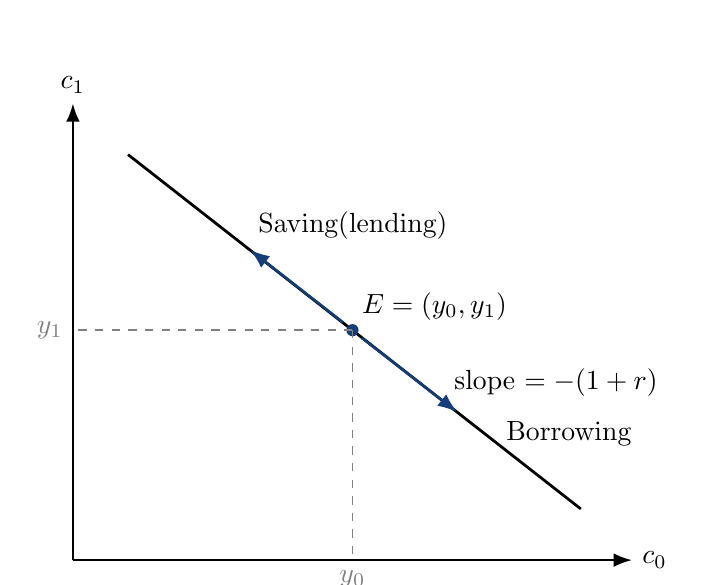
\begin{tikzpicture}[
  >=Latex,
  axis/.style={-Latex, line width=0.8pt},
  budget/.style={line width=1.0pt},
  guide/.style={dashed, gray, line width=0.6pt},
  move/.style={-Latex, line width=0.9pt, FinanceBlue}
]
\draw[axis] (0,0) -- (7.1,0) node[right] {$c_0$};
\draw[axis] (0,0) -- (0,5.8) node[above] {$c_1$};
\draw[budget] (0.7,5.15) -- (6.45,0.65);
\coordinate (E) at (3.55,2.92);
\fill[FinanceBlue] (E) circle (2.2pt);
\node[above right] at (E) {$E=(y_0,y_1)$};
\draw[guide] (E) -- (3.55,0) node[below] {$y_0$};
\draw[guide] (E) -- (0,2.92) node[left] {$y_1$};
\draw[move] (3.43,3.02) -- (2.25,3.94);
\node[above left, align=center] at (4.88,3.95) {Saving(lending)};
\draw[move] (3.67,2.82) -- (4.88,1.88);
\node[below right] at (5.38,1.88) {Borrowing};
\node[above right] at (4.72,1.95) {slope $=-(1+r)$};
\end{tikzpicture}
\caption{Saving, borrowing, and the intertemporal budget constraint}
\label{fig:ch1-intertemporal-budget}
\end{figure}

At the endowment point $E$, consumption equals income in each period. Moving up and to the left means consuming less than current income and shifting purchasing power into the future. Moving down and to the right means borrowing against future income. The budget line shows that the timing of income need not determine the timing of consumption.

For firms, having investment opportunities does not necessarily imply having the financial resources needed to pursue them. A firm may have a valuable project but insufficient internal funds, while outside investors have resources available for investment. As Figure~\ref{fig:ch1-internal-external-finance} shows, external finance bridges this separation by bringing outside resources into the firm in exchange for claims on future payments.
\begin{figure}[H]
\centering
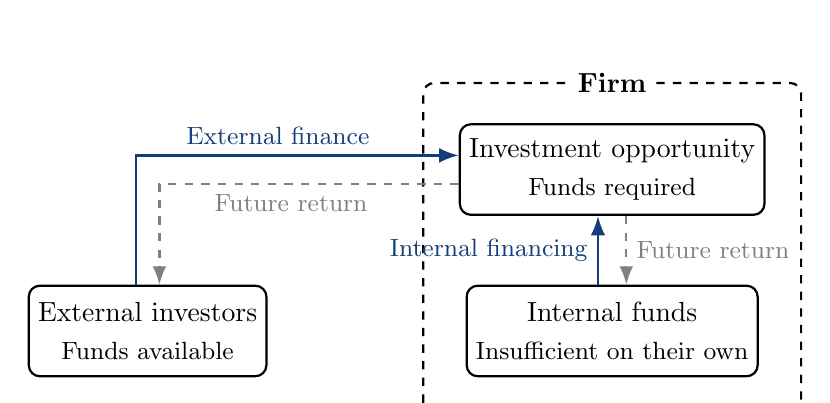
\begin{tikzpicture}[
  >=Latex,
  box/.style={
    draw,
    rounded corners,
    minimum width=3.0cm,
    minimum height=1.15cm,
    align=center,
    line width=0.8pt
  },
  flow/.style={
    -Latex,
    line width=0.9pt,
    FinanceBlue
  },
  return/.style={
    -Latex,
    dashed,
    line width=0.8pt,
    gray
  },
  firmbox/.style={
    draw,
    rounded corners,
    dashed,
    line width=0.8pt
  }
]

%------------------------------------------------
% External investors
%------------------------------------------------
\node[box] (outside) at (0.3,1.3)
{External investors\\[2pt]
\small Funds available};

%------------------------------------------------
% Firm
%------------------------------------------------
\node[box] (internal) at (6.2,1.3)
{Internal funds\\[2pt]
\small Insufficient on their own};

\node[box] (project) at (6.2,3.35)
{Investment opportunity\\[2pt]
\small Funds required};

% Firm boundary
\draw[firmbox]
  (3.8,0.25) rectangle (8.6,4.45);

\node[
  fill=white,
  inner sep=2pt,
  font=\bfseries
]
at (6.2,4.45) {Firm};

%------------------------------------------------
% Internal financing and future return
%------------------------------------------------

% Current financing: slightly left
\coordinate (intfinstart)
  at ($(internal.north)+(-0.18,0)$);

\coordinate (intfinend)
  at ($(project.south)+(-0.18,0)$);

\draw[flow]
  (intfinstart)
  -- node[left, font=\small]
  {Internal financing}
  (intfinend);

% Future return: slightly right
\coordinate (intreturnstart)
  at ($(project.south)+(0.18,0)$);

\coordinate (intreturnend)
  at ($(internal.north)+(0.18,0)$);

\draw[return]
  (intreturnstart)
  -- node[right, font=\small]
  {Future return}
  (intreturnend);

%------------------------------------------------
% External financing and future return
%------------------------------------------------

% External finance: upper path
\coordinate (extfinstart)
  at ($(outside.north)+(-0.15,0)$);

\coordinate (extfinend)
  at ($(project.west)+(0,0.18)$);

\draw[flow]
  (extfinstart)
  |- node[pos=0.72, above, font=\small]
  {External finance}
  (extfinend);

% Future return: lower parallel path
\coordinate (extreturnstart)
  at ($(project.west)+(0,-0.18)$);

\coordinate (extreturnend)
  at ($(outside.north)+(0.15,0)$);

\draw[return]
  (extreturnstart)
  -| node[pos=0.28, below, font=\small]
  {Future return}
  (extreturnend);

\end{tikzpicture}

\caption{Internal and external finance when resources and investment opportunities are separated}
\label{fig:ch1-internal-external-finance}
\end{figure}


\subsection{Uncertainty and the Allocation of Risk}

Intertemporal exchange becomes more difficult because the future is uncertain. Knight distinguished risk from uncertainty according to what is known about future outcomes \cite{Knight1921}. Risk refers to situations in which the possible future states are known and the probability of each state can be specified. Uncertainty, by contrast, arises in two situations. In the first, the possible future states are known, but their probabilities are unknown. In the second, the possible future states themselves cannot be fully identified, and their probabilities are therefore also unknown.

Financial arrangements can determine how the economic consequences of different states are distributed among participants. They do not eliminate the underlying uncertainty about which state will occur, but they can change who bears the resulting gains and losses.

Risk allocation may create economic value when participants differ in their exposure to risk and in their ability or willingness to bear it. Financial arrangements can transfer risk toward participants better able or more willing to bear particular exposures. Risk sharing is one form of this allocation: losses that would be difficult for one individual to absorb may instead be distributed across many participants.

If total resources available in state $s$ are $Y(s)$ and participant $i$ receives $X_i(s)$, any feasible allocation must satisfy

\begin{equation}
\sum_i X_i(s)=Y(s)
\qquad \text{for every state }s.
\label{eq:ch1_risk_sharing}
\end{equation}

The constraint means that risk sharing can change the distribution of resources within a state, but not the total resources available in that state. Figure~\ref{fig:ch1-risk-sharing} illustrates this distinction.

\begin{figure}[H]
\centering
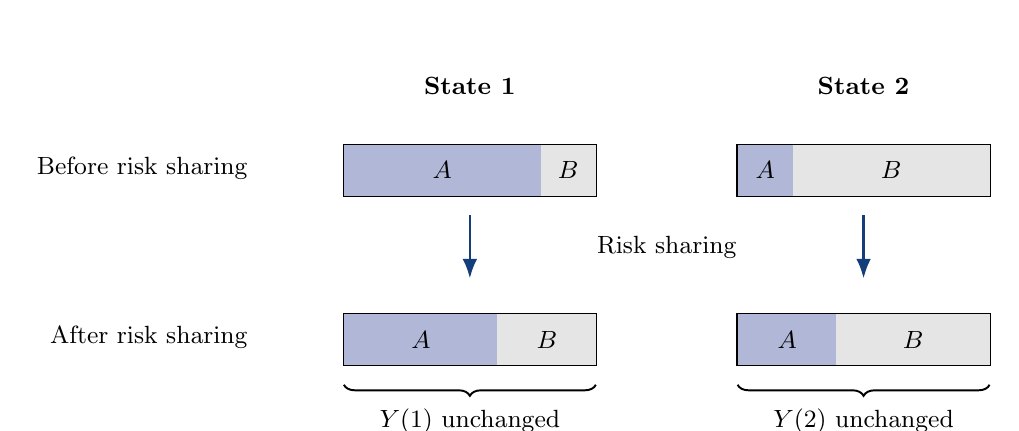
\begin{tikzpicture}[
  >=Latex,
  title/.style={font=\small\bfseries},
  label/.style={font=\small},
  flow/.style={-Latex, line width=0.9pt, FinanceBlue},
  total/.style={draw, line width=0.8pt, minimum height=0.65cm},
  abar/.style={fill=FinanceBlue!25},
  bbar/.style={fill=gray!20}
]

%------------------------------------------------
% Column headings
%------------------------------------------------
\node[title] at (3.0,5.2) {State 1};
\node[title] at (8.0,5.2) {State 2};

%------------------------------------------------
% Before risk sharing
%------------------------------------------------
\node[label, anchor=east] at (0.3,4.15)
{Before risk sharing};

% State 1: A has more, B has less
\draw[total] (1.4,3.8) rectangle (4.6,4.45);
\fill[abar] (1.4,3.8) rectangle (3.9,4.45);
\fill[bbar] (3.9,3.8) rectangle (4.6,4.45);

\node[label] at (2.65,4.125) {$A$};
\node[label] at (4.25,4.125) {$B$};

% State 2: A has less, B has more
\draw[total] (6.4,3.8) rectangle (9.6,4.45);
\fill[abar] (6.4,3.8) rectangle (7.1,4.45);
\fill[bbar] (7.1,3.8) rectangle (9.6,4.45);

\node[label] at (6.75,4.125) {$A$};
\node[label] at (8.35,4.125) {$B$};

%------------------------------------------------
% Risk-sharing arrows
%------------------------------------------------
\draw[flow] (3.0,3.55) -- (3.0,2.75);
\draw[flow] (8.0,3.55) -- (8.0,2.75);

\node[label, fill=white, inner sep=2pt]
  at (5.5,3.15) {Risk sharing};

%------------------------------------------------
% After risk sharing
%------------------------------------------------
\node[label, anchor=east] at (0.3,2.0)
{After risk sharing};

% State 1: more balanced allocation
\draw[total] (1.4,1.65) rectangle (4.6,2.30);
\fill[abar] (1.4,1.65) rectangle (3.35,2.30);
\fill[bbar] (3.35,1.65) rectangle (4.6,2.30);

\node[label] at (2.38,1.975) {$A$};
\node[label] at (3.98,1.975) {$B$};

% State 2: more balanced allocation
\draw[total] (6.4,1.65) rectangle (9.6,2.30);
\fill[abar] (6.4,1.65) rectangle (7.65,2.30);
\fill[bbar] (7.65,1.65) rectangle (9.6,2.30);

\node[label] at (7.03,1.975) {$A$};
\node[label] at (8.63,1.975) {$B$};

%------------------------------------------------
% Aggregate resource labels
%------------------------------------------------
\draw[decorate,
  decoration={brace, amplitude=4pt, mirror},
  line width=0.7pt]
  (1.4,1.40) -- (4.6,1.40)
  node[midway, below=5pt, label] {$Y(1)$ unchanged};

\draw[decorate,
  decoration={brace, amplitude=4pt, mirror},
  line width=0.7pt]
  (6.4,1.40) -- (9.6,1.40)
  node[midway, below=5pt, label] {$Y(2)$ unchanged};

\end{tikzpicture}

\caption{Risk sharing changes allocation, not aggregate resources}
\label{fig:ch1-risk-sharing}
\end{figure}

Given the resources available in each state, finance can redistribute the consequences of risk but cannot eliminate an aggregate loss. Insurance pools losses across policyholders, equity distributes business risk among investors, derivatives reallocate particular exposures, and diversification reduces dependence on idiosyncratic outcomes. Risk allocation therefore concerns who bears economic consequences in different states of the world.

\subsection{Information and Incentive Frictions}

Financial decisions require assessments of projects, counterparties, and future cash flows before outcomes are realized. The information underlying these assessments is often incomplete and unevenly distributed among participants.

Such differences in information constitute information asymmetry. Firm managers may possess more information about project quality than outside investors, while borrowers may have private information about actions that lenders cannot directly observe. Before financing, unobservable differences in project quality can give rise to adverse selection when financing terms affect which borrowers seek or accept funding. After financing, moral hazard may arise when borrowers have incentives to take actions that affect lenders' payoffs but cannot be fully observed.

These problems cannot be resolved by disclosure alone. Information may be costly to produce, difficult to verify, and incomplete even when it is available. Financial systems devote resources to screening, auditing, certification, monitoring. These activities improve the information on which financial decisions are based, although they cannot eliminate uncertainty about future outcomes.

\begin{tcolorbox}[
  enhanced,
  breakable,
  colback=white,
  colframe=FinanceBlue,
  boxrule=0.7pt,
  sharp corners,
  borderline west={2.2pt}{0pt}{FinanceBlue},
  title=\textbf{Finance Perspective: Why Financial Contracts Do More Than Transfer Funds},
  coltitle=white,
  colbacktitle=FinanceBlue,
  fonttitle=\bfseries,
  before skip=1.2em,
  after skip=1.2em
]
Before funds are provided, lenders and investors may evaluate borrowers, issuers, or projects, verify financial information, and use credit histories or reputation. Lenders may also require collateral. After financing, contracts may require periodic disclosure, restrict certain actions, and grant rights to monitor performance or intervene when contractual conditions are breached.

These mechanisms do not eliminate information asymmetry. Screening and verification are used primarily before financing, when relevant characteristics may be difficult to observe. Disclosure, monitoring, and contractual restrictions become important after financing, when actions may be difficult to observe.
\end{tcolorbox}

Information affects both whether financing occurs and the terms on which it is offered. But information does not by itself define the rights and obligations of the parties. Those rights and obligations must be specified, and future promises must be credible and enforceable.


\subsection{Commitment and Enforcement}

Many financial arrangements rely on contracts that specify future commitments, rights, and obligations. Contracts define payments, contingencies, and remedies when agreed terms are not met. A debt contract, for example, specifies when payments are due and what rights creditors have if the borrower defaults.

Contractual commitments are credible only to the extent that parties expect future obligations to be honored. A commitment problem arises when a party cannot credibly bind its future behavior at the time the contract is written. After financing, a party may have incentives to take actions that benefit itself while reducing the value of another party's claim. Collateral, covenants, reputation, and control rights can support commitment by restricting certain actions or altering the consequences of nonperformance.

Enforcement gives contractual rights practical force. Courts, creditor rights, bankruptcy procedures, and collateral arrangements determine the remedies available when obligations are breached. Expectations about enforcement influence whether financing is provided and on what terms. Yet enforcement is neither complete nor costless: contracts cannot specify every future contingency, and legal proceedings may be costly or slow. Financial arrangements also rely on renegotiation, reputation, and discretion alongside formal contractual rights.

These four economic problems often arise together. For example, a bank loan transfers purchasing power across time, allocates risks associated with uncertain repayment, depends on information about the borrower, and establishes contractual rights and obligations supported by enforcement mechanisms. Financial arrangements thus typically address several economic problems simultaneously.

\section{What a Financial System Does}

The economic problems discussed above provide the rationale for the core functions of a financial system. Although financial systems vary across countries and over time, they allocate resources across time and alternative uses, share and transform risk, provide liquidity and support payments, produce information and discipline behavior, and facilitate price discovery. These functions remain relevant even as the institutions and technologies through which they are performed change.

\subsection{Allocating Resources Across Time and Alternative Uses}

Finance reallocates purchasing power across dates. Borrowing allows individuals to bring future purchasing power forward, while saving and investment transfer current purchasing power into the future. Over the life cycle, these arrangements can help finance education or housing early in adulthood, accumulate resources during the working years, and support consumption after retirement. For firms, financing similarly allows investment to take place before the cash flows generated by a project are realized.

\begin{figure}[H]
\centering
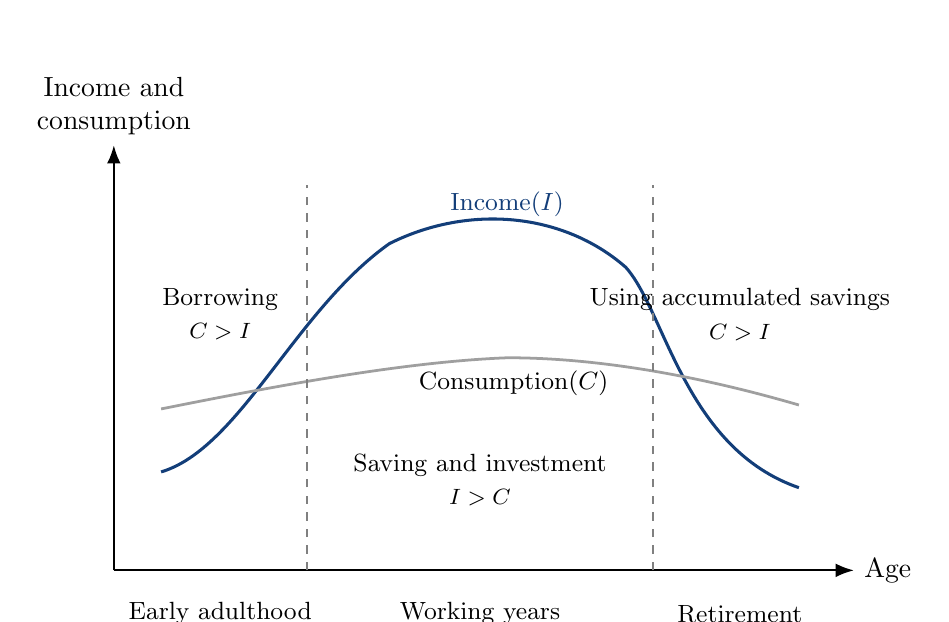
\begin{tikzpicture}[
  >=Latex,
  axis/.style={-Latex, line width=0.8pt},
  income/.style={line width=1.1pt, FinanceBlue},
  consumption/.style={line width=1.0pt, gray!75},
  guide/.style={dashed, gray, line width=0.6pt},
  label/.style={font=\small}
]

%------------------------------------------------
% Axes
%------------------------------------------------
\draw[axis] (0,0) -- (9.4,0) node[right] {Age};
\draw[axis] (0,0) -- (0,5.4)
  node[above, align=center] {Income and\\consumption};

%------------------------------------------------
% Income over the life cycle
%------------------------------------------------
\draw[income]
  (0.6,1.25)
  .. controls (1.6,1.55) and (2.3,3.3) ..
  (3.5,4.15)
  .. controls (4.5,4.65) and (5.7,4.55) ..
  (6.5,3.85)
  .. controls (7.0,3.3) and (7.25,1.55) ..
  (8.7,1.05);

%------------------------------------------------
% Consumption over the life cycle
%------------------------------------------------
\draw[consumption]
  (0.6,2.05)
  .. controls (2.1,2.35) and (3.7,2.65) ..
  (5.0,2.70)
  .. controls (6.2,2.70) and (7.5,2.45) ..
  (8.7,2.10);

%------------------------------------------------
% Curve labels
%------------------------------------------------
\node[label, FinanceBlue, anchor=west]
  at (4.15,4.65) {Income($I$)};

\node[label, anchor=west]
  at (3.75,2.38) {Consumption($C$)};

%------------------------------------------------
% Stage separators
%------------------------------------------------
\draw[guide] (2.45,0) -- (2.45,4.9);
\draw[guide] (6.85,0) -- (6.85,4.9);

%------------------------------------------------
% Stage labels
%------------------------------------------------
\node[label, align=center] at (1.35,-0.55)
  {Early adulthood};

\node[label, align=center] at (4.65,-0.55)
  {Working years};

\node[label, align=center] at (7.95,-0.55)
  {Retirement};

%------------------------------------------------
% Financial allocation labels
%------------------------------------------------
\node[label, align=center] at (1.35,3.25)
  {Borrowing\\[1pt]
   \footnotesize $C > I$};

\node[label, align=center] at (4.65,1.15)
  {Saving and investment\\[1pt]
   \footnotesize $I > C$};

\node[label, align=center] at (7.95,3.25)
  {Using accumulated savings\\[1pt]
   \footnotesize $C > I$};

\end{tikzpicture}

\caption{Financial allocation over the life cycle}
\label{fig:ch1-life-cycle-allocation}
\end{figure}

Figure~\ref{fig:ch1-life-cycle-allocation} illustrates this role over the life cycle. Income and spending needs may follow different paths, so borrowing and saving can shift purchasing power between different stages of life.

Finance also allocates scarce resources among competing uses. Interest rates, security prices, lending decisions, and investment mandates influence which projects receive funding and on what terms. If two firms compete for limited funds, a project offering a more favorable expected return relative to its risk and financing cost may receive more financing or better terms, while another may receive less or none.

\subsection{Sharing and Transforming Risk}

Participants differ in the risks they face and in their capacity or willingness to bear them. These differences create scope for reallocating risk across participants. A loss that would be large relative to one participant's resources may be easier for another to absorb, or may become less burdensome when distributed across many participants or combined with other exposures. Financial arrangements can share risk across participants or transform the form in which that risk is borne.
\begin{figure}[H]
\centering
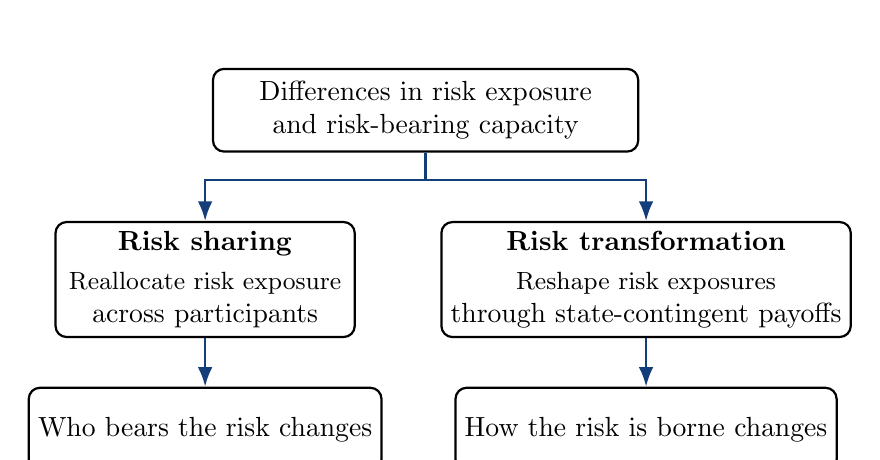
\begin{tikzpicture}[
  >=Latex,
  box/.style={
    draw,
    rounded corners,
    minimum width=3.8cm,
    minimum height=1.05cm,
    align=center,
    line width=0.8pt
  },
  topbox/.style={
    draw,
    rounded corners,
    minimum width=5.4cm,
    minimum height=1.05cm,
    align=center,
    line width=0.8pt
  },
  flow/.style={
    -Latex,
    line width=0.9pt,
    FinanceBlue
  },
  note/.style={
    font=\small,
    align=center
  }
]

%------------------------------------------------
% Source of risk reallocation
%------------------------------------------------
\node[topbox] (heterogeneity) at (5.5,4.6)
{Differences in risk exposure\\
and risk-bearing capacity};

%------------------------------------------------
% Risk sharing
%------------------------------------------------
\node[box] (sharing) at (2.7,2.45)
{\textbf{Risk sharing}\\[2pt]
\small Reallocate risk exposure\\
across participants};

\node[box] (sharingout) at (2.7,0.55)
{Who bears the risk changes};

%------------------------------------------------
% Risk transformation
%------------------------------------------------
\node[box] (transform) at (8.3,2.45)
{\textbf{Risk transformation}\\[2pt]
\small Reshape risk exposures \\through state-contingent payoffs};

\node[box] (transformout) at (8.3,0.55)
{How the risk is borne changes};

%------------------------------------------------
% Branching arrows from common source
%------------------------------------------------
\coordinate (split)
  at ($(heterogeneity.south)+(0,-0.35)$);

% Common stem
\draw[line width=0.9pt, FinanceBlue]
  (heterogeneity.south) -- (split);

% Left branch: Risk sharing
\draw[flow]
  (split)
  -| (sharing.north);

% Right branch: Risk transformation
\draw[flow]
  (split)
  -| (transform.north);

\draw[flow]
  (sharing.south)
  -- (sharingout.north);

\draw[flow]
  (transform.south)
  -- (transformout.north);

\end{tikzpicture}

\caption{Risk sharing and risk transformation}
\label{fig:ch1-risk-sharing-transformation}
\end{figure}

Risk sharing changes the distribution of exposure across participants. Insurance, for example, pools specified losses across many policyholders. Risk transformation reshapes risk exposures through financial claims with different payoffs across future states. Debt and equity, for example, divide a firm's cash flows into senior and residual claims, while derivatives create payoffs linked to changes in prices, interest rates, or other underlying variables.


\subsection{Providing Liquidity and Supporting Payments}

Liquidity concerns the ability to meet payment obligations as they fall due and the ease with which assets can be converted into purchasing power without significant delay or loss of value. The demand for liquidity arises when cash inflows and payment obligations are not perfectly synchronized. Financial arrangements bridge this timing gap by making funds available when needed.

For example, a solvent firm may hold valuable assets but little cash. If those assets cannot be sold quickly without a substantial price concession, market liquidity is limited; if the firm cannot borrow against them or obtain short-term financing, funding liquidity is also limited.

Cash and other liquid assets help meet payment obligations, while payment and settlement systems enable the transfer of funds and the settlement of obligations.

Liquidity provision may involve maturity and liquidity transformation. Banks, for example, fund longer-term, less liquid loans with deposits available on demand. This structure provides liquidity to depositors but creates a mismatch between liquid liabilities and less liquid assets, which can become a source of fragility when withdrawals or funding needs rise.

\subsection{Producing Information and Disciplining Behavior}

Financial decisions depend on information about expected cash flows, risk, and the incentives of the parties involved. Before resources are committed, information must be produced, interpreted, and compared. Screening, financial analysis, auditing, credit assessment, and market trading all contribute to this process. In markets, prices also incorporate information revealed through the decisions of many participants.

Information remains important after financing. Monitoring provides evidence about performance and the use of funds, while governance arrangements and financing terms influence subsequent decisions and incentives. Financial systems do not simply allocate resources on the basis of existing information; they also produce information and create mechanisms that discipline behavior when information is incomplete.

\subsection{Discovering Prices}

Financial systems generate prices through trading. Valuation provides estimates based on expected cash flows, timing, risk, and contingencies, while market prices are formed through the interaction of buyers and sellers. Participants act on different information, beliefs, constraints, and objectives. Their trading decisions influence demand and supply, leading to price adjustments. As new information and transactions enter the market, prices continue to change, making price discovery an ongoing process.

The resulting prices enter subsequent financial decisions. Interest rates influence saving, borrowing, and financing costs; bond yields and equity prices affect issuance and investment; exchange rates alter the domestic value of foreign cash flows; and asset prices affect collateral and borrowing capacity. Financial prices therefore transmit information from trading into later economic decisions.

\section{How the Financial System Is Organized}

The financial system performs these functions through several interconnected components. These include money and payment systems, financial markets, financial institutions, and financial instruments. Although analytically distinct, these components interact in practice.

\subsection{Money, Payments, and Settlement}

Financial transactions create obligations that must eventually be discharged. Their discharge requires an accepted means of payment. Money provides a common unit for expressing financial obligations and a means through which those obligations can be settled.

The transfer of money through payment systems may involve clearing and settlement. Clearing determines the obligations arising from transactions and may reduce them through netting, while settlement completes payment through the transfer of an accepted settlement asset. Together, money, payment arrangements, clearing, and settlement provide the institutional basis through which financial obligations are discharged.

\subsection{Financial Markets}

Financial markets organize the issuance and exchange of financial claims and provide mechanisms for price formation. The issuance of new securities enables firms, governments, and other borrowers to obtain funds from investors, while secondary-market trading reallocates existing claims and risk exposures. Prices emerge from transactions among participants with different information, beliefs, and constraints and inform subsequent financing and investment decisions.

Market exchange, however, does not eliminate the costs of evaluating counterparties, producing and verifying information, designing contracts, and monitoring performance. Nor do direct transactions always meet the needs of participants seeking delegated investment, risk pooling, or liquidity and maturity transformation. 

\subsection{Financial Institutions}

Financial institutions perform financial functions through specialized organizations rather than through direct market exchange alone. Specialization can reduce the costs of producing information, executing transactions, managing risks, and monitoring financial relationships. Banks, asset managers, insurers, and other intermediaries combine these functions through different forms of pooling, transformation, and delegation.

Through these activities, intermediation affects the allocation of information, control, and risk within financial relationships. Delegation may create agency problems when decisions are made on behalf of others, while maturity, liquidity, and risk transformation may create exposures that require management within the institution. Governance, contractual arrangements, and regulation therefore influence both the performance of financial functions and the risks associated with intermediation.

\subsection{Financial Instruments}

Financial instruments specify how future cash flows, risks, and rights are allocated among participants. Debt defines promised payments and creditor priority, while equity assigns residual claims and often voting rights. Insurance and derivatives make payments contingent on specified losses, prices, rates, or other future events.

The allocation created by an instrument depends on its contractual terms. Maturity, seniority, collateral, covenants, margin requirements, and embedded options determine when payments occur, how losses are absorbed, and when control rights may shift. A financial instrument is defines rights and obligations governing the allocation ofcash flows, risk, and control across time and future states.

\par\medskip
\noindent
Table~\ref{tab:ch1-architecture} summarizes how these organizational forms support the financial functions discussed in the previous section.

\begin{table}[H]
\centering

\caption{Organizational forms of the financial system}
\label{tab:ch1-architecture}

\begin{tabularx}{\textwidth}{@{}p{3.0cm}X X@{}}
\toprule
\textbf{Form}
&
\textbf{Organizes}
&
\textbf{Main functions}
\\
\midrule

Money, payments, and settlement
&
The discharge and transfer of obligations
&
Payments and liquidity
\\

Financial markets
&
The exchange of claims and risks
&
Allocation, liquidity, price discovery
\\

Financial institutions
&
Specialized intermediation and delegation
&
Information, liquidity, risk sharing
\\

Financial instruments
&
Cash flows, rights, and exposures
&
Allocation, risk transformation, incentives
\\

\bottomrule
\end{tabularx}

\end{table}

\section{Finance and the Real Economy}

Finance affects which economic choices are feasible for households, firms, and governments. It influences which projects are undertaken, how consumption is allocated over time, how shocks are absorbed, and how disturbances propagate through balance sheets and markets.

\subsection{Capital Formation and Economic Development}

Finance supports capital formation by channeling available resources toward productive investment. This process involves identifying viable investment opportunities, arranging financing, monitoring the use of funds, and allocating the associated risks.

A firm may identify a viable investment opportunity before its retained earnings are sufficient to finance it. By issuing financial claims on future cash flows, the firm can obtain purchasing power today and use it to acquire productive assets.

At the aggregate level, the contribution of finance to economic development depends not only on the volume of financing but also on how the financial system allocates capital, structures incentives, and allocates risk. More financing does not necessarily translate into more productive investment.

\subsection{Financial Innovation and Access}

Financial innovation changes the way financial functions are performed by altering transaction costs, information requirements, contractual structures, or the transferability of claims. Lower costs of payment, verification, trading, or risk transfer can make transactions feasible that were previously too costly or difficult to arrange.

These changes may broaden access to financial services for households and firms that face high fixed costs, limited collateral, or weak connections to traditional intermediaries. Greater access help relax constraints on payments, saving, borrowing, investment, and risk management, allowing a wider range of economic activities to be financed or undertaken.

The contribution of financial innovation to economic development depends on which financial frictions it relaxes and how the resulting changes in access affect economic activity. Lower transaction or information costs, for example, may enable productive investment or risk sharing that would otherwise be too costly to arrange. Greater access alone, however, does not ensure more productive investment if innovation weakens screening, facilitates excessive leverage, or directs funds toward less productive uses.



\begin{figure}[H]
\centering
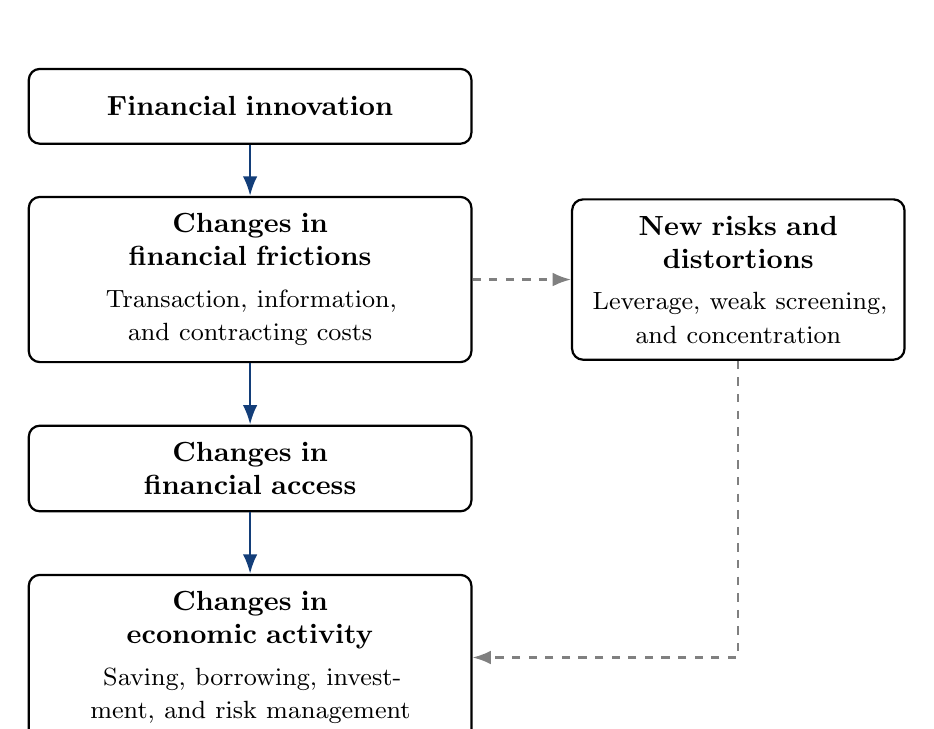
\begin{tikzpicture}[
  >=Latex,
  box/.style={
    draw,
    rounded corners,
    text width=5.2cm,
    minimum height=0.95cm,
    align=center,
    inner sep=6pt,
    line width=0.8pt
  },
  sidebox/.style={
    draw,
    rounded corners,
    text width=3.8cm,
    minimum height=0.95cm,
    align=center,
    inner sep=6pt,
    line width=0.8pt
  },
  flow/.style={
    -Latex,
    line width=0.9pt,
    FinanceBlue
  },
  sideflow/.style={
    -Latex,
    dashed,
    line width=0.8pt,
    gray
  }
]

\node[box] (innovation) at (0,4.2)
  {\textbf{Financial innovation}};

\node[box] (frictions) at (0,2.0)
  {\textbf{Changes in \\financial frictions}\\[3pt]
   \small Transaction, information, and contracting costs};

\node[box] (access) at (0,-0.4)
  {\textbf{Changes in \\financial access}};

\node[box] (activity) at (0,-2.8)
  {\textbf{Changes in \\economic activity}\\[3pt]
   \small Saving, borrowing, investment, and risk management};

\node[sidebox] (risks) at (6.2,2.0)
  {\textbf{New risks and distortions}\\[3pt]
   \small Leverage, weak screening, and concentration};

\draw[flow] (innovation.south) -- (frictions.north);
\draw[flow] (frictions.south) -- (access.north);
\draw[flow] (access.south) -- (activity.north);

\draw[sideflow] (frictions.east) -- (risks.west);
\draw[sideflow]
  (risks.south) |- (activity.east);

\end{tikzpicture}

\caption{Financial innovation, access, and real economic activity}
\label{fig:ch1-innovation-access}
\end{figure}

\subsection{Fragility and Financial Amplification}

The arrangements that make finance useful can also create fragility. Leverage magnifies gains and losses, liquidity transformation creates mismatches between assets and liabilities, and market-based adjustment can become destabilizing when many participants respond in similar ways. Risk transfer may disperse exposures, but it can also make their ultimate location more difficult to identify.

Financial fragility often arises from feedback effects rather than from a single loss. A decline in asset prices can reduce collateral values, tighten borrowing constraints, and force asset sales. Those sales may depress prices further, weakening collateral and credit conditions again. Figure~\ref {fig:ch1-fragility-loop} illustrates this amplification mechanism.

As financial conditions tighten, these effects spread to real economic activity. Firms facing weaker collateral and more limited access to credit may reduce investment, while households facing tighter borrowing conditions or losses in wealth may reduce consumption. Financial amplification can turn an initial disturbance into a broader contraction in spending and production.

\begin{figure}[H]
\centering
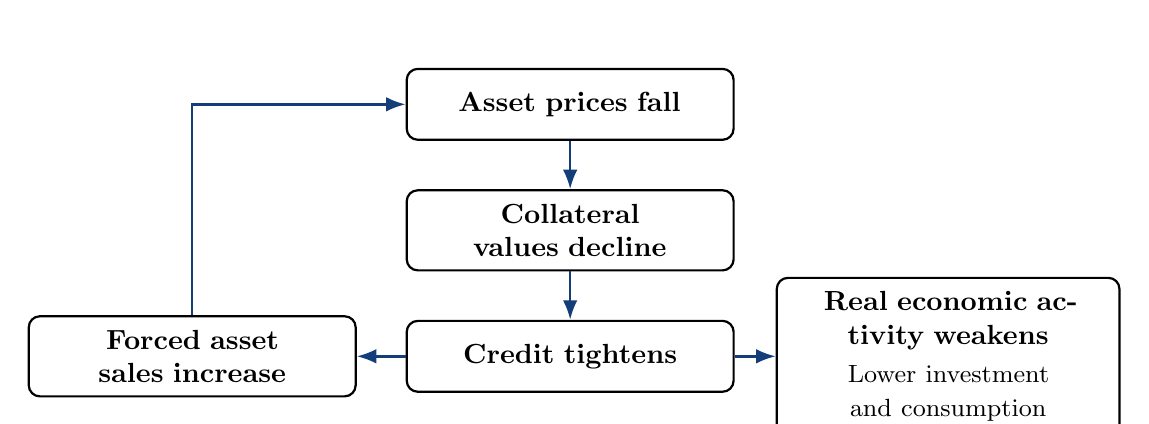
\begin{tikzpicture}[
  >=Latex,
  box/.style={
    draw,
    rounded corners,
    text width=3.8cm,
    minimum height=0.9cm,
    align=center,
    inner sep=5pt,
    line width=0.8pt
  },
  realbox/.style={
    draw,
    rounded corners,
    text width=4.0cm,
    minimum height=0.9cm,
    align=center,
    inner sep=5pt,
    line width=0.8pt
  },
  flow/.style={
    -Latex,
    line width=0.9pt,
    FinanceBlue
  }
]

% Financial amplification loop
\node[box] (prices) at (0,3.6)
  {\textbf{Asset prices fall}};

\node[box] (collateral) at (0,2.0)
  {\textbf{Collateral \\values decline}};

\node[box] (credit) at (0,0.4)
  {\textbf{Credit tightens}};

\node[box] (sales) at (-4.8,0.4)
  {\textbf{Forced asset sales increase}};

% Real-economy effect
\node[realbox] (real) at (4.8,0.4)
  {\textbf{Real economic activity weakens}\\[2pt]
   \small Lower investment and consumption};

% Main financial loop
\draw[flow] (prices.south) -- (collateral.north);
\draw[flow] (collateral.south) -- (credit.north);
\draw[flow] (credit.west) -- (sales.east);
\draw[flow] (sales.north) |- (prices.west);

% Transmission to the real economy
\draw[flow] (credit.east) -- (real.west);

\end{tikzpicture}

\caption{Financial amplification and transmission to the real economy}
\label{fig:ch1-fragility-loop}
\end{figure}

\section{A Functional Perspective on a Changing Financial System}

Technological change can alter who performs financial functions, how those functions are combined, and the organizational forms through which they are carried out. Activities may shift among banks, markets, digital platforms, and technological infrastructures; information-processing tasks may increasingly be supported or performed by algorithms; and financial claims may be issued, traded, or settled in new ways. Such changes can substantially alter the organization of finance without eliminating the underlying need to allocate resources, produce information, manage risk, provide liquidity, and support credible financial obligations.

Artificial intelligence illustrates this distinction. AI can change how screening, monitoring, trading, and financial decisions are performed, while the use of common data, models, or decision rules may also create new forms of concentration and interdependence. Digital platforms, programmable contracts, tokenized assets, and new payment arrangements can produce similar shifts in organizational form. They may change the boundaries between markets, intermediaries, and infrastructure, or alter how financial claims are created, transferred, and settled. 

\TailModule{summary}{Summary}

Financial exchange often separates resources available today from spending and investment opportunities that arise at other dates. Even when future outcomes are known, this separation creates a role for saving, borrowing, and financing. When future outcomes are uncertain, decisions also depend on information that may be incomplete or unevenly distributed, while contracts and institutions help define rights and obligations and make future commitments credible and enforceable.

Finance expand economic possibilities by supporting investment, risk sharing, and access to financial services, but the same arrangements can also generate fragility. Leverage magnifies losses, liquidity transformation creates funding mismatches, and individually rational responses may interact through prices and balance sheets to amplify shocks across the financial system. Artificial intelligence, digital platforms, and other technologies can alter the costs and organizational forms through which financial functions are performed without eliminating the economic problems that give rise to those functions.

\TailModule{keyterms}{Key Terms}

Intertemporal exchange; risk sharing;
adverse selection; moral hazard; commitment; enforcement; capital allocation;
monetary liquidity; market liquidity; funding liquidity; information production;
price discovery; financial intermediation; financial fragility

\TailModule{aiprompt}{Financial AI Lab}

\textbf{Lab: Follow the Function}

Choose one financial innovation or digital financial service. Ask an AI
system to explain what makes it ``new.'' Then reorganize the answer around
the analytical framework used in this chapter: the underlying economic
problem, the financial function involved, the organizational form through
which it is performed, the allocation of cash flows and risks, and the
conditions under which the arrangement could fail. Identify factual claims
that require external verification and any part of the AI answer that
mistakes technological novelty for a change in economic function.

\TailModule{questions}{Discussion Questions}

\begin{enumerate}
\item Why can intertemporal exchange create a role for finance even when future outcomes are known with certainty?
\item How does uncertainty make information economically valuable, and why is information alone insufficient to support financial exchange?
\item Why can a financial arrangement address several economic problems at the same time? Illustrate with a bank loan, insurance contract, or traded security.
\item Why can liquidity provision improve economic efficiency and also create financial fragility?
\end{enumerate}

\TailModule{appprobs}{Applied Problems}

\begin{enumerate}
\item An individual has income of 40 today and 66 next period. The borrowing and lending rate is 10\%. Use equation~\eqref{eq:ch1_intertemporal_budget} to find next-period consumption if current consumption is 50. Is the individual borrowing or saving, and by how much today?

\item A financial intermediary funds five-year loans largely with liabilities redeemable on demand. Explain the economic benefit of this structure in normal times and the mechanism through which it can become unstable during stress. Identify the financial function being provided and the source of fragility.
\end{enumerate}

\TailModule{furtherread}{Further Reading}

\begin{itemize}

\item Merton, Robert C. (1995),
``A Functional Perspective of Financial Intermediation,''
\emph{Financial Management}, 24(2), 23--41.

\item Merton, Robert C., and Zvi Bodie (1995),
``A Conceptual Framework for Analyzing the Financial Environment,''
in Dwight B. Crane et al., \emph{The Global Financial System:
A Functional Perspective}, Harvard Business School Press, pp.~3--31.

\item Levine, Ross (2005),
``Finance and Growth: Theory and Evidence,''
in Philippe Aghion and Steven N. Durlauf (eds.),
\emph{Handbook of Economic Growth}, Vol.~1A,
Elsevier, pp.~865--934.

\end{itemize}

\ChapterTail{summary,keyterms,aiprompt,questions,appprobs,furtherread}

\chapter{Money, Payments, and Liquidity Architecture}
\label{chap:Money_Payments_and_Liquidity_Architecture}

\begin{openingcase}[Historical Case Based on Public Information]{A Payment App Is Not the Settlement Asset}

By the late 2010s, mobile and online payments had become deeply embedded in everyday commerce in China. To a user, the transaction often appeared simple: open an app, scan a code, confirm the amount, and the payment is complete. Behind that interface, however, the institutional path of the payment was changing.

Non-bank payment institutions had previously connected directly with many commercial banks to process online payments involving bank accounts. The People's Bank of China required payment institutions to break these direct connections and route the relevant transactions through centralized clearing infrastructures. By January 14, 2019, payment businesses jointly conducted by non-bank payment institutions and commercial banks were processed through NetsUnion Clearing or China UnionPay.\footnote{People's Bank of China, \emph{Annual Report 2018}, section on payment system development and the establishment of NetsUnion Clearing.}

For most customers, the payment experience remained largely unchanged, even as the institutional architecture behind it changed substantially.

\end{openingcase}

%========================================================
% Core Questions
%========================================================

\begin{tcolorbox}[
  enhanced,
  colback=FinanceBlue!6,
  colframe=FinanceBlue,
  boxrule=0.6pt,
  sharp corners,
  left=8pt,
  right=8pt,
  top=7pt,
  bottom=7pt,
  before skip=1em,
  after skip=1.6em,
  title=\textbf{Core Questions},
  coltitle=white,
  colbacktitle=FinanceBlue,
  fonttitle=\bfseries,
  attach boxed title to top left={xshift=6pt,yshift=-2mm},
  boxed title style={
    boxrule=0pt,
    sharp corners,
    left=5pt,
    right=5pt,
    top=2pt,
    bottom=2pt
  }
]
\begin{enumerate}[
  leftmargin=*,
  label=\textcolor{FinanceBlue}{\textbf{\arabic*.}},
  itemsep=0.55em,
  topsep=0.2em
]
\item What makes some financial claims function as money while others do not?
\item How are payment instructions processed through clearing and settlement, and when is a payment final?
\item Why do modern monetary systems rely on both central bank money and commercial bank money, and what supports their convertibility at par?
\end{enumerate}
\end{tcolorbox}

\section{Money as a Financial Agreement}

Why would one person accept a particular object or account balance from another in exchange for goods, labor, or financial claims? The answer depends not only on the form of money, but also on the institutions that make it widely acceptable and usable for settling obligations. 

\subsection{Money as a Social and Institutional Arrangement}

Money's usefulness depends on a shared expectation that others will accept it in payment. If every seller had to check an issuer's backing, legal status, and the asset's acceptability before taking it in payment, ordinary exchange would become costly. Money reduces this burden by creating a commonly accepted unit and settlement convention.

This property is partly self-reinforcing. An asset becomes more useful for payment as more people accept it, and wider acceptance gives others a stronger reason to hold and use it. This feedback generates network effects in monetary exchange. But these alone are not enough. Participants must also trust that the monetary unit will remain usable and that payments made in it will be recognized and settled.
Modern monetary systems support this confidence through law, payment infrastructure, central-bank arrangements, regulation, and shared expectations. 

Money is not merely a social convention. Its use depends on both collective acceptance and the institutional arrangements that support monetary claims. For example, a bank deposit is an asset for the depositor and a liability for the issuing bank. The general acceptability of money therefore rests not only on shared expectations but also on the arrangements that support payment and settlement.

\subsection{The Core Functions of Money}

Once a monetary claim is widely accepted and institutionally supported, it can perform three core monetary functions.

The \emph{unit of account} provides a common language for prices and financial obligations. A loan agreement can specify RMB~1 million rather than a changing bundle of goods. A bond can promise coupon and principal payments in the same unit used to record the issuer's revenues and the investor's wealth. Without a common unit, comparison and contracting become more costly.

The \emph{medium of exchange} function allows money to facilitate transactions and discharge obligations. Cash can settle a face-to-face transaction directly. A bank deposit can be transferred through a payment system. 


\begin{table}[H]
\centering
\caption{The Core Functions of Money}
\label{tab:ch2-money-functions}
\renewcommand{\arraystretch}{1.4}
\begin{tabularx}{\textwidth}{
    @{}
    >{\raggedright\arraybackslash}p{3.0cm}
    >{\raggedright\arraybackslash}X
    >{\raggedright\arraybackslash}X
    @{}
}
\toprule
\textbf{Function}
& \textbf{Economic role}
& \textbf{Financial significance} \\
\midrule

Unit of account
& Provides a common measure for prices and obligations
& Makes contracts, accounting, and valuation comparable \\

Medium of exchange
& Facilitates transactions and discharges obligations
& Enables efficient exchange of goods and services \\

Store of value
& Carries purchasing power across time
& Allows wealth to be held in a liquid, nominal form \\

\bottomrule
\end{tabularx}
\end{table}

The \emph{store of value} function allows purchasing power to be carried across time. Money is not a perfect store of value because inflation can reduce its real purchasing power. Even so, it is often more stable and liquid than many other assets. 

These functions provide a useful way to distinguish money from other financial assets and payment instruments.For example, a government bond may be a good store of value without serving as a medium of exchange. A payment card facilitates transactions but is not itself money: a debit card provides access to a bank deposit, while a credit card allows the holder to draw on a credit facility. A foreign currency may perform the functions of money in one jurisdiction while being held mainly as a financial asset in another.


\subsection{The Balance-Sheet Structure of Money}

Most money in a modern economy takes the form of financial claims recorded on institutional balance sheets. The most important forms are commercial-bank deposits, central-bank reserves, and currency, although they differ in who can hold them and how they are used.

Commercial-bank deposits are liabilities of banks and assets of depositors. Central-bank reserves are liabilities of the central bank and assets of eligible account holders, principally banks and other designated institutions. Currency is also recorded as a liability of the central bank, although modern fiat currency is not generally redeemable for gold or another specified asset at a fixed rate.

\begin{table}[H]
\centering
\caption{A Bank Deposit as an Asset and a Liability}
\label{tab:ch2-deposit-taccount}

\renewcommand{\arraystretch}{1.25}

\begin{tabularx}{0.9\textwidth}{
    @{}
    >{\raggedright\arraybackslash}X
    >{\raggedright\arraybackslash}X
    >{\raggedright\arraybackslash}X
    @{}
}
\toprule
\multicolumn{1}{c}{\textbf{Household}}
&
\multicolumn{2}{c}{\textbf{Commercial Bank}}
\\
\cmidrule(r){1-1}
\cmidrule(l){2-3}

\textbf{Assets}
&
\textbf{Assets}
&
\textbf{Liabilities}
\\

Bank deposit: RMB~100
&
--
&
Bank deposit: RMB~100
\\

\bottomrule
\end{tabularx}
\end{table}

Table~\ref{tab:ch2-deposit-taccount} illustrates how the same RMB~100 deposit appears on two balance sheets: as an asset of the household and a liability of the bank.

The balance-sheet perspective clarifies why different forms of money are not economically identical. 
An RMB~100 bank deposit and an RMB~100 banknote share the same unit of account and are normally accepted at par, but they have different issuers and balance-sheet relationships. The deposit is a liability of a commercial bank and an asset of the depositor, whereas the banknote is a liability of the central bank and an asset of its holder.

\begin{table}[H]
\centering
\caption{Selected Monetary Forms and Their Balance-Sheet Positions}
\label{tab:ch2-money-claims}

\renewcommand{\arraystretch}{1.15}
\setlength{\tabcolsep}{7pt}

\begin{tabularx}{\textwidth}{
    @{}
    >{\raggedright\arraybackslash}p{3.35cm}
    >{\raggedright\arraybackslash}p{2.85cm}
    >{\raggedright\arraybackslash}X
    @{}
}
\toprule
\textbf{Monetary form}
& \textbf{Issuer}
& \textbf{Balance-sheet relationship} \\
\midrule

Currency\newline
{\small (banknotes and coins)}
& Central bank
& Liability of the central bank; asset held by the public \\
\addlinespace[0.3em]

Central-bank reserves
& Central bank
& Liability of the central bank; asset of eligible account holders \\
\addlinespace[0.3em]

Commercial-bank deposits
& Commercial bank
& Liability of the bank; asset of the depositor \\

\bottomrule
\end{tabularx}
\end{table}

The same balance-sheet logic helps explain how commercial-bank deposits are created. Suppose a bank grants a new loan of RMB~100 and credits the borrower's deposit account by the same amount. On the bank's balance sheet,

\begin{equation}
\Delta \text{Loans}=+100,
\qquad
\Delta \text{Deposits}=+100.
\label{eq:ch2-loan-deposit}
\end{equation}

The loan therefore creates a new bank deposit at origination. The borrower simultaneously acquires a deposit asset and a matching loan liability, so there is no equal increase in net wealth. Deposit creation remains subject to the bank's broader balance-sheet and regulatory constraints.

\subsection{Trust, Credibility, and Monetary Stability}

Money reduces information costs by limiting the need to reassess the issuer behind each monetary claim in every transaction. A recipient of a bank transfer typically relies on the transferability of the deposit rather than assessing the payer's bank, while a holder of currency does not need to examine the central bank's balance sheet. The efficiency of monetary exchange rests on the ability to treat accepted monetary claims as reliable without repeated verification.

Such trust rests on the credibility of the institutions and arrangements that support the monetary system. The monetary unit needs to remain sufficiently stable to support pricing and contracting, and monetary claims need to be transferable or convertible as promised. Reliable payment systems and legal rules that define ownership and settlement finality also support this credibility.

A decline in monetary trust can affect behavior in several ways. If depositors become concerned about a bank's ability to meet withdrawals, they may convert deposits into currency or transfer funds to other banks. If confidence in a privately issued monetary claim weakens, the claim may trade below par or lose acceptance. If inflation undermines confidence in the unit of account, households and firms may shorten contract maturities, index prices, or shift toward other currencies or assets.

Monetary stability also depends on the expectation that different forms of money denominated in the same unit will remain interchangeable. This expectation supports common pricing, contracting, and payment across the economy.

\section{Payment Systems and Financial Networks}

Money can serve as a means of payment only if it can be transferred between users. A payment system is the set of instruments, rules, institutions, technologies, and settlement arrangements through which funds are transferred and monetary obligations are discharged.

\subsection{Payment Instruments and Traditional Payment Infrastructure}

Payment instruments are the means through which payment instructions are initiated and transmitted. Cash combines the payment instrument and the settlement asset in a single object: handing over currency can complete the transaction directly. Most non-cash payments separate the payment instruction from the asset used for settlement.

Non-cash payment instruments differ in who initiates the payment and how the instruction is transmitted. Cheques and credit transfers are payer-initiated, whereas direct debits are payee-initiated under prior authorization. Card and mobile payments rely on payment networks and digital interfaces to authenticate users, authorize transactions, and route payment instructions. 

\begin{figure}[H]
\centering

\resizebox{0.94\textwidth}{!}{%
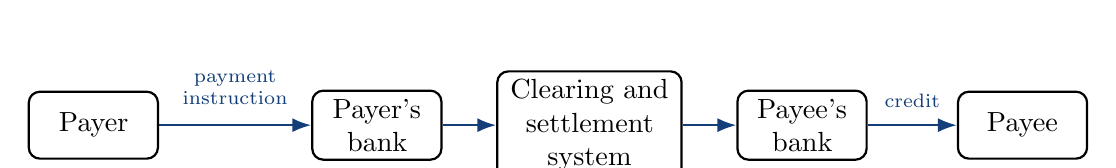
\begin{tikzpicture}[
  >=Latex,
  box/.style={
  draw,
  rounded corners,
  align=center,
  minimum height=0.85cm,
  text width=1.5cm,
  inner xsep=2pt,
  inner ysep=3pt,
  line width=0.8pt
  },
  flow/.style={
    -Latex,
    line width=0.85pt,
    FinanceBlue
  },
  note/.style={
    font=\scriptsize,
    align=center,
    text=FinanceBlue,
    fill=white,
    inner sep=1pt
  }
]

\node[box] (payer) at (0,0) {Payer};
\node[box] (bankA) at (3.6,0) {Payer's bank};
\node[box, text width=2.2cm] (infra) at (6.3,0)
{Clearing and\\settlement system};

\node[box] (bankB) at (9.0,0) {Payee's bank};
\node[box] (payee) at (11.8,0) {Payee};

\draw[flow] (payer) -- 
  node[midway, above=6pt, note]{payment\\ instruction}
  (bankA);

\draw[flow] (bankA) -- (infra);

\draw[flow] (infra) -- (bankB);

\draw[flow] (bankB) -- 
  node[midway, above=5pt, note]{credit}
  (payee);

\end{tikzpicture}%
}

\caption{A Simplified Cross-Bank Payment Chain}
\label{fig:ch2-payment-chain}
\end{figure}

Figure~\ref{fig:ch2-payment-chain} illustrates a simplified cross-bank payment chain. If the payer and payee use the same bank, the transaction can be settled internally by reducing one deposit account and increasing another. If they use different banks, the payment creates an interbank obligation. The participating banks must then settle with each other, typically using a settlement asset accepted by both.

A payment network is thereforemore than a communication system. Its design affects when obligations arise and are discharged, how much liquidity participants require, and the credit and operational exposures they face before settlement becomes final.

\subsection{Clearing, Netting, and Payment Obligations}

Clearing is the process through which payment instructions are transmitted, reconciled, confirmed, and converted into obligations for settlement. Where applicable, these obligations may be netted before settlement.

Consider a set of banks indexed by $i$ and $j$. Let $p_{ij}$ denote the amount that bank $i$ must pay bank $j$. Bank $i$'s gross outgoing payments are

\begin{equation}
G_i^{\mathrm{out}}
=\sum_{j\neq i} p_{ij},
\label{eq:ch2-gross-outgoing}
\end{equation}
while its net settlement position can be written as

\begin{equation}
N_i=\sum_{j\neq i} p_{ij}-\sum_{j\neq i} p_{ji}.
\label{eq:ch2-net-position}
\end{equation}

A positive $N_i$  represents a net payment obligation, while a negative value represents a net receipt. In a closed clearing system,

\begin{equation}
\sum_i N_i=0.
\label{eq:ch2-net-zero}
\end{equation}

Netting can substantially reduce the liquidity required for settlement. Suppose Bank A owes Bank B 100, Bank B owes Bank C 90, and Bank C owes Bank A 80. Table~\ref{tab:ch2-netting-example} shows the resulting gross flows and net settlement positions.

\begin{table}[H]
\centering
\caption{Gross payments and net settlement positions}
\label{tab:ch2-netting-example}
\begin{tabular}{@{}lrrr@{}}
\toprule
\textbf{Bank} & \textbf{Outgoing} & \textbf{Incoming} & \textbf{Net position} \\
\midrule
A & 100 & 80 & Pays 20 \\
B & 90 & 100 & Receives 10 \\
C & 80 & 90 & Receives 10 \\
\bottomrule
\end{tabular}
\end{table}

The three gross payments total 270, but after multilateral netting the system has only 20 of aggregate net debit obligations to settle. Bank A pays 20, while Banks B and C receive 10 each. Netting reduces the liquidity required for settlement.

In deferred net settlement systems, these liquidity savings come with a cost. Payment obligations may remain unsettled until the end of the clearing cycle, exposing participants to the risk of another participant's default. Payment-system design involves a trade-off between liquidity efficiency, settlement finality, and risk containment.

\subsection{Settlement, Payment Finality, and Settlement Risk}

Settlement is the discharge of payment obligations through transfers on the books of a settlement institution. Payment finality refers to the point at which a payment is regarded as complete and cannot be revoked under the applicable system rules and law.

The distinction between clearing and settlement can be seen in a simple cross-bank transfer. Suppose a customer at Bank A pays RMB~100 to a customer at Bank B. If the payment is settled in central-bank reserves, the essential balance-sheet changes are shown in Table~\ref{tab:ch2-cross-bank-payment}.

\begin{table}[H]
\centering
\caption{Balance-Sheet Effects of a Cross-Bank Payment of RMB~100}
\label{tab:ch2-cross-bank-payment}

\renewcommand{\arraystretch}{1.2}

\begin{tabularx}{\textwidth}{
    @{}
    >{\raggedright\arraybackslash}p{3.0cm}
    >{\raggedright\arraybackslash}X
    >{\raggedright\arraybackslash}X
    @{}
}
\toprule
\textbf{Institution}
& \textbf{Assets}
& \textbf{Liabilities} \\
\midrule

Bank A
& Reserves $-100$
& Payer's deposit $-100$ \\

Bank B
& Reserves $+100$
& Payee's deposit $+100$ \\

Central bank
& ---
& Reserve liability to Bank A $-100$; reserve liability to Bank B $+100$ \\

\bottomrule
\end{tabularx}
\end{table}

The transfer of reserves from Bank A to Bank B settles the interbank obligation. The customer's deposit does not physically move from one bank to another. Instead, Bank A reduces its liability to the payer, Bank B increases its liability to the payee, and central-bank reserves are transferred between the two banks. Settlement finality is reached when that settlement becomes irrevocable and unconditional under the rules of the system.

A settlement asset should allow obligations to be discharged without introducing significant additional credit risk at the point of settlement. Central-bank money is widely used for settlement in systemically important domestic payment systems.

Before settlement finality is reached, participants remain exposed to settlement risk: the expected settlement may be delayed or fail to occur. Such failures can generate several related forms of risk, summarized in Table~\ref     {tab:ch2-payment-risk}.

\begin{table}[H]
\centering
\caption{Major Forms of Payment-System Risk}
\label{tab:ch2-payment-risk}

\renewcommand{\arraystretch}{1.2}

\begin{tabularx}{\textwidth}{
    @{}
    >{\raggedright\arraybackslash}p{3.0cm}
    >{\raggedright\arraybackslash}X
    @{}
}
\toprule
\textbf{Risk}
& \textbf{Economic meaning} \\
\midrule


Credit risk
& A participant may fail to meet an obligation in full, either when due or at any time thereafter. \\

Liquidity risk
& A participant may be unable to meet an obligation when due but may settle it in full at a later time. \\

Operational risk
& Technology failures, cyber incidents, human error, or infrastructure disruptions may interrupt processing or settlement \\

Legal risk
& Uncertainty about rules, ownership, netting, or finality may undermine enforceability \\

\bottomrule
\end{tabularx}
\end{table}

The importance of these risks depends partly on how settlement is organized. In a real-time gross settlement system, payments are settled individually and continuously, reducing the duration of interbank exposures but increasing intraday liquidity needs. In a deferred net settlement system, obligations are accumulated and netted before settlement, reducing liquidity needs but leaving exposures outstanding for longer.

Settlement design involves a trade-off between liquidity efficiency, the speed of finality, and risk containment.

\subsection{Digital Payment Networks and Platforms}

Digitalization changes how payments are initiated, authenticated, and routed, but it does not remove the need to distinguish monetary claims, clearing, and settlement. A mobile wallet or payment app may make payment appear instantaneous to the user, yet the underlying value may still be a bank deposit, a regulated payment claim, or another monetary asset. The essential question is not only how the payment is made, but what claim is being transferred and how final settlement occurs.

A payment network connects users, merchants, financial institutions, payment service providers, and clearing or settlement infrastructures. Its value depends not only on technology, but also on participation, interoperability, rules, and trust. A larger network can make payments easier and cheaper, but it can also create dependence on a small number of platforms or infrastructures.

\begin{figure}[H]
\centering

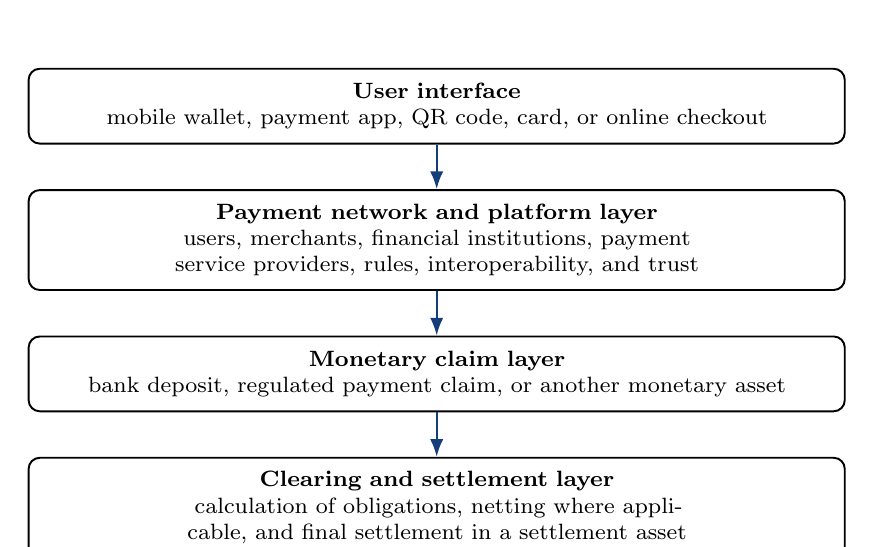
\begin{tikzpicture}[
  >=Latex,
  layer/.style={
    draw,
    rounded corners,
    align=center,
    minimum height=0.95cm,
    text width=0.82\textwidth,
    inner xsep=6pt,
    inner ysep=5pt,
    line width=0.7pt,
    font=\footnotesize
  },
  arrow/.style={
    -Latex,
    line width=0.75pt,
    FinanceBlue
  }
]

\node[layer] (interface) at (0,2.4)
{\textbf{User interface}\\
mobile wallet, payment app, QR code, card, or online checkout};

\node[layer] (network) at (0,0.7)
{\textbf{Payment network and platform layer}\\
users, merchants, financial institutions, payment service providers, rules, interoperability, and trust};

\node[layer] (claim) at (0,-1.0)
{\textbf{Monetary claim layer}\\
bank deposit, regulated payment claim, or another monetary asset};

\node[layer] (settlement) at (0,-2.7)
{\textbf{Clearing and settlement layer}\\
calculation of obligations, netting where applicable, and final settlement in a settlement asset};

\draw[arrow] (interface) -- (network);
\draw[arrow] (network) -- (claim);
\draw[arrow] (claim) -- (settlement);

\end{tikzpicture}

\caption{Digital Payment as Interface, Network, Claim, and Settlement Layers}
\label{fig:ch2-digital-payment-layers}
\end{figure}

Figure~\ref{fig:ch2-digital-payment-layers} illustrates that digital payment involves more than a change in user interface. The same visible payment may rest on different underlying monetary claims, network arrangements, and settlement assets.

Within this layered architecture, the platform layer coordinates interactions among users, merchants, banks, and payment service providers. Through access management, authentication, transaction routing, and data processing, platforms can reduce transaction costs and processing delays. These arrangements also generate network effects: the value of a payment service to participants may increase with the number of users and merchants, creating economies of scale while potentially reinforcing market concentration. Payment data can improve fraud detection and service design, but its collection and use raise concerns about privacy, market power, interoperability, and access.

The same logic applies to newer payment technologies. 
Programmable transfers and tokenized claims may bring trading, clearing, and settlement closer together by embedding conditions in transaction logic. Artificial intelligence can improve fraud detection, transaction monitoring, liquidity forecasting, and payment routing. Yet faster execution and better prediction do not by themselves establish legal finality, guarantee par redemption, or eliminate liquidity needs. The economic problem remains institutional as well as computational.

\section{Liquidity in the Monetary System}

Money can serve as a means of payment only when monetary claims can be used, transferred, or converted as obligations come due. Payment systems therefore require not only monetary assets but also liquidity: the ability to obtain the required settlement asset when needed.

\subsection{Liquidity, Convertibility, and Economic Exchange}

Liquidity is distinct from an asset's value. It describes how readily an asset can be used to meet payment or settlement obligations when they come due. Currency can discharge many retail payments directly. A government security may be valuable and actively traded, but its value usually must be converted into spendable funds through a sale or collateralized borrowing before it can support an ordinary payment. The difference lies in the distance between holding value and making payment.

Convertibility may reduce this distance. Here, convertibility refers to the ability to convert one monetary claim into another, typically at par and without significant delay. A bank deposit is a private liability of a commercial bank, but it can function as money in ordinary exchange when it is both convertible into currency at par and transferable through payment networks.

The importance of convertibility becomes apparent when confidence in par redemption weakens. Depositors may then withdraw cash or move balances to other institutions. More generally, a payment claim that cannot be reliably redeemed at its stated value may cease to circulate as a close substitute for money.

Convertibility, however, does not eliminate the importance of timing. Suppose a bank expects a large inflow at 4:00 p.m. but must make a payment at 10:00 a.m. Even if its end-of-day position would be balanced, it still needs liquidity at 10:00 a.m. This timing mismatch creates a demand for reserves, intraday credit, and other arrangements that make settlement assets available when needed.


\begin{tcolorbox}[
  enhanced,
  breakable,
  colback=white,
  colframe=FinanceBlue,
  boxrule=0.7pt,
  sharp corners,
  borderline west={2.2pt}{0pt}{FinanceBlue},
 title=\textbf{Financial Perspective: Convertibility Is Not Liquidity},
  coltitle=white,
  colbacktitle=FinanceBlue,
  fonttitle=\bfseries,
  before skip=1.2em,
  after skip=1.2em
]
Convertibility concerns whether a financial claim can be exchanged for a usable payment or settlement asset, typically at par. Liquidity additionally requires that the relevant asset be available in the required amount and at the required time. A claim may therefore be convertible in principle without providing sufficient liquidity when an obligation falls due.
\end{tcolorbox}

At the system level, the same temporal mismatch can generate payment gridlock. Institutions may postpone outgoing payments in anticipation of incoming funds. When such behavior is widespread, settlement can be delayed even if aggregate liquidity is sufficient over the course of the day. Liquidity arrangements must therefore ensure not only an adequate quantity of settlement assets, but also their timely availability across participants.

Maintaining liquidity entails an opportunity cost. Reserves and other highly liquid assets provide immediate settlement capacity but may offer lower returns than less liquid alternatives. Financial institutions therefore face a trade-off between liquidity and return, holding sufficient liquid assets to meet obligations while allocating other funds to higher-yielding uses.

This trade-off reflects the broader role of liquidity and convertibility in economic exchange. By reducing the need to liquidate other assets before payment and limiting delays in the discharge of obligations, they lower transaction frictions and support the circulation of monetary claims across the economy.

\subsection{Safe Assets and the Demand for Liquidity}

The demand for liquidity helps explain the distinctive role of safe assets in the monetary system. Safe and liquid assets can be mobilized to meet payment and settlement needs while limiting exposure to credit loss.

Safety is conceptually distinct from liquidity. Here, safety refers primarily to credit quality: a safe asset carries a low risk that its promised payments will not be made in full and on time. Liquidity concerns the ease with which an asset can be used or mobilized to meet payment or settlement obligations when they fall due.

Safety alone does not determine an asset's liquidity. Its liquidity also depends on whether it can be readily sold or pledged on favorable terms, particularly under stressed market conditions.

Liquidity and collateral services are also reflected in asset yields. Among otherwise comparable assets, investors may accept a lower yield on one that provides more valuable liquidity or collateral services. The value attached to these services is commonly described as a convenience yield.

\begin{equation}
y
=
y^{*}-\lambda,
\qquad \lambda>0,
\label{eq:ch2-convenience-yield}
\end{equation}
where $y^{*}$ is the yield on an otherwise comparable asset that does not provide the same convenience services, and $\lambda$ represents the convenience yield associated with liquidity, collateral, and related services. This expression is an economic decomposition rather than a pricing model, and $\lambda$ may vary with market conditions.

The demand for safe and liquid assets often increases during periods of uncertainty or financial stress. Market participants may reduce their holdings of riskier claims and shift toward cash, short-term government securities, or, for eligible institutions, central-bank reserves. Such a flight to safety may reduce individual risk exposure while tightening funding conditions and market liquidity elsewhere.

At the institutional level, efforts to preserve liquidity can amplify stress. If institutions simultaneously reduce lending, conserve settlement assets, or sell less-liquid securities, funding conditions may tighten and asset-market liquidity may deteriorate. Actions that are prudent for individual institutions can  contribute to system-wide liquidity stress.

When such behavior becomes widespread, the demand for liquidity becomes a system-wide coordination problem. A resilient monetary system requires arrangements that support the mobilization and distribution of liquidity as conditions change. Central-bank liquidity facilities, collateral frameworks, and payment-system arrangements form part of this institutional architecture.


\section{The Architecture of Public and Private Money}
Modern monetary systems comprise monetary liabilities issued on interconnected public and private balance sheets. Central-bank money provides a common settlement foundation, while commercial-bank deposits account for much of the money used in everyday economic activity.

\subsection{Public Money and the Central Bank}

Public money in modern monetary systems consists primarily of central-bank liabilities: currency in circulation and reserve balances maintained by institutions with access to central-bank accounts. Both are denominated in the common unit of account, but they perform different functions within the payment and settlement system.

The central bank issues these liabilities and maintains the reserve accounts used for interbank settlement. When one participating institution makes a payment to another, reserve balances are transferred between their accounts at the central bank. This transfer reallocates central-bank liabilities across institutions and extinguishes the corresponding interbank obligation. Settlement in central-bank money therefore does not require an additional claim on a private settlement intermediary.

\subsection{Private Money and Commercial Banks}

Private money in modern monetary systems consists primarily of commercial-bank deposits. Each deposit is an asset of the depositor and a liability of the issuing bank. Deposits used as money are denominated in the common unit of account and transferable through the payment system. Although deposits issued by different banks share the same unit of account, each remains a claim on a particular institution.

Commercial banks create deposits when they expand their balance sheets. When a bank grants a loan, it records the loan as an asset and credits the borrower's deposit account by the same amount, creating a new deposit liability at the same time. Deposit creation does not require an equivalent quantity of central-bank money to be supplied in advance.

Deposit creation is nevertheless subject to financial and institutional constraints. Banks must maintain adequate capital and liquidity, manage credit risk, and remain able to meet payment and settlement obligations as their balance sheets expand.

A key feature of modern monetary systems is that deposits issued by different banks are separate legal liabilities, yet they are ordinarily accepted at the same nominal value. This equivalence depends on the arrangements that connect commercial-bank deposits to central-bank money and support convertibility at par.

\subsection{Par Convertibility and the Hierarchy of Money}

Different monetary claims may be denominated in the same unit of account even though they are liabilities of different issuers. An RMB~100 deposit at one commercial bank is legally distinct from an RMB~100 deposit at another bank and from RMB~100 in currency. Par convertibility means that these forms of money can normally be exchanged at par rather than at market-determined discounts or premia.

Par convertibility preserves nominal equivalence without eliminating differences among issuers. Commercial-bank deposits remain claims on individual banks, whereas currency and reserve balances are liabilities of the central bank. 

These differences are reflected in a hierarchy of money. Commercial-bank deposits can be used for most payments by households and firms, whereas interbank obligations are typically settled in central-bank money. The hierarchy therefore reflects differences in issuer and settlement status rather than differences in the unit of account.

This hierarchy is compatible with monetary unity as long as par convertibility is maintained. When confidence in convertibility weakens, differences among issuers become economically significant and the unity of the monetary system may begin to break down.

\subsection{Maintaining the Unity of the Monetary System}

Par convertibility allows legally distinct monetary liabilities to be used at a common nominal value. Maintaining this monetary unity depends on the ability of private issuers to honor their liabilities and on the availability of liquidity for settlement. Weakness in either condition can disrupt the par relationship among monetary claims.

The first condition concerns the financial soundness of the issuing bank. Prudential regulation and supervision constrain risk-taking and require adequate capital, reducing the likelihood that a bank will be unable to honor its deposit liabilities. If a bank fails, deposit insurance protects covered deposits, while resolution arrangements provide an orderly process for handling the failed institution. These mechanisms help preserve confidence that commercial-bank deposits will be honored at par.

The second condition concerns settlement liquidity. Cross-bank payments generate interbank obligations that must be settled in a timely manner. Reserve balances held at the central bank serve as the settlement asset, while liquidity facilities can provide additional reserves when temporary shortages arise. Common payment rules, interoperability, and settlement finality support reliable cross-bank payments and help maintain par convertibility.

Together, these arrangements allow legally distinct monetary liabilities to function as equivalent forms of money within a common monetary system.

%========================================================
% Summary
%========================================================

\TailModule{summary}{Summary}

Money is more than a widely accepted asset. It provides a common unit of account, supports exchange, and carries purchasing power across time. In modern monetary systems, most forms of money are also financial claims. Currency and central-bank reserves are liabilities of the central bank, while commercial-bank deposits are liabilities of individual banks. Their usefulness depends on trust, transferability, and the institutional arrangements that support payment and settlement.

Payments involve more than the transfer of an instruction. Clearing determines the obligations that arise among participants, netting can reduce the amount that must be settled, and settlement discharges those obligations through an accepted settlement asset. The timing and finality of settlement affect both liquidity needs and financial risk. Digital payment technologies can change how payments are initiated, authenticated, and routed without removing these underlying economic functions.

Liquidity concerns the ability to meet payment and settlement obligations when they fall due. Convertibility allows monetary claims to be exchanged at par, while safe and liquid assets provide additional liquidity and collateral services. These services can affect asset yields and become especially valuable during periods of financial stress.

Modern monetary systems combine public and private money. Commercial banks create deposit money through balance-sheet expansion, while central-bank money provides a common basis for interbank settlement. Par convertibility allows legally distinct monetary claims to function at a common nominal value. Maintaining this monetary unity requires financially sound issuers, adequate settlement liquidity, reliable payment infrastructure, and institutions capable of managing bank distress.

%========================================================
% Key Terms
%========================================================

\TailModule{keyterms}{Key Terms}

Money; unit of account; medium of exchange; payment system; clearing; netting; settlement; settlement finality; liquidity; convertibility; safe asset; convenience yield; central-bank money; commercial-bank money; par convertibility; hierarchy of money

%========================================================
% Discussion Questions
%========================================================

\TailModule{aiprompt}{Financial AI Lab}

\textbf{Lab: Trace the Payment to Final Settlement}

Select a payment method that can be documented from reliable sources, such as a bank transfer, bank card, QR-code payment, or digital wallet. Ask an AI system to describe the complete transaction path from the payer's instruction to final settlement. Treat the generated answer as a hypothesis to be verified rather than as an authoritative description.

Reconstruct the transaction using five checks: identify the monetary claim held by the payer; identify the institution that issues that claim; identify the clearing arrangement; identify the asset used for final settlement; and identify the rule or institution that determines settlement finality. For each step, require a verifiable institutional source and mark any statement that cannot be confirmed.

Compare the verified transaction path with the AI-generated answer. Identify any point at which the AI confuses the payment interface with the underlying monetary claim, clearing process, balance-sheet transfer, or settlement asset. Conclude by explaining which parts of the payment process are technological and which depend on financial and institutional arrangements.

%========================================================
% Further Reading
%========================================================

\TailModule{questions}{Discussion Questions}

\begin{enumerate}

\item Why is a mobile payment application not necessarily the same as the asset used to settle a payment? What monetary claims may underlie a digital payment?

\item In a deferred net settlement system, why can netting reduce liquidity requirements while leaving participants exposed to settlement risk?

\item Why can commercial-bank deposits function as money even though they are liabilities of private institutions? What institutional arrangements support their acceptance at par?

\item During periods of financial stress, why might households or financial institutions shift from bank deposits to currency, deposits at other banks, or other liquid assets? What does this behavior reveal about differences among monetary claims?

\end{enumerate}

%========================================================
% Applied Problems
%========================================================

\TailModule{appprobs}{Applied Problems}

\begin{enumerate}

\item Four banks have the following payment obligations at the end of a clearing cycle: A owes B 120; B owes C 100; C owes D 70; D owes A 60; and A owes C 30. Calculate each bank's gross outgoing payments, gross incoming payments, and net settlement position. What is the total value of payments if all obligations are settled gross? After full multilateral netting, which banks are net debtors and net creditors, and what is the total amount that must be transferred by net debtors to complete settlement?

\item A customer at Bank X transfers RMB~50,000 to a customer at Bank Y. Show the balance-sheet changes for Bank X, Bank Y, and the central bank when the interbank obligation is settled in reserve balances. Then explain how the balance-sheet effects would differ if both customers held accounts at Bank X.

\item Two otherwise comparable one-year securities have the same expected cash flows and comparable credit risk. Security A yields 3.2\% and is eligible as collateral for intraday central-bank credit, whereas Security B yields 3.8\% and is not. Using equation~\eqref{eq:ch2-convenience-yield}, interpret the 0.6 percentage-point yield difference. What assumptions are required before this difference can be attributed entirely to liquidity and collateral services?

\end{enumerate}

%========================================================
% Data Application
%========================================================

\TailModule{dataapp}{Data Application}

\textbf{Payment Architecture in the Data: China, 2024}

The People's Bank of China reports that in 2024 the High-Value Payment System processed 392 million transactions with a total value of RMB~8,824.18 trillion, while the NetsUnion Clearing platform processed about 1.03 trillion transactions with a total value of RMB~520.53 trillion.\footnote{People's Bank of China, \emph{Payment System Operations in 2024}, Section III, Payment Systems.}

\begin{enumerate}

\item Calculate the average transaction value processed by each system.

\item Compare transaction volume with transaction value. What do these
two measures reveal about the different economic roles of the two systems?

\item Relate these differences to the payment-system mechanisms discussed
in this chapter. Why would a high-value real-time payment system place
particular importance on settlement liquidity and finality, while a
platform processing very large numbers of relatively small transactions
places greater emphasis on processing capacity and low unit cost?

\item Repeat the comparison using a later People's Bank of China
payment-system report. How have the volume, value, and average transaction
size of the two systems changed? Before drawing conclusions, examine
whether the statistical definitions or coverage have changed.

\end{enumerate}

%========================================================
% Financial AI Lab
%========================================================

\TailModule{furtherread}{Further Reading}
\begin{itemize}

\item People's Bank of China (2025), \emph{Payment System Report (2024)}.

\item McLeay, Michael, Amar Radia, and Ryland Thomas (2014),
``Money in the Modern Economy: An Introduction,''
\emph{Bank of England Quarterly Bulletin}, 54(1), 4--13.

\item Committee on Payment and Settlement Systems and
Technical Committee of the International Organization of Securities
Commissions (2012), \emph{Principles for Financial Market Infrastructures},
Bank for International Settlements.

\item Bank for International Settlements (2025),
``The Next-Generation Monetary and Financial System,''
Chapter III in \emph{BIS Annual Economic Report 2025}.

\end{itemize}

%========================================================
% Tail row in Full Contents
%========================================================

\ChapterTail{summary,keyterms,aiprompt,questions,appprobs,dataapp,furtherread}


\part{Information, Contracts, and Valuation}
\chapter{Information Economics and Financial Contracts}
\label{chap:Information_Economics_and_Financial_Contracts}

\begin{openingcase}{Why Can a Higher Interest Rate Reduce Lending?}

Suppose Huaxin Commercial Bank is reviewing loan applications from two manufacturing firms, Rongda Machinery and Xinhai Technologies. On paper, the two firms look much alike. Their revenues, leverage, collateral, and recent financial performance are broadly similar. Yet their investment projects are very different.

Rongda plans to expand an established production line. Its expected return is modest, but the project has a relatively high probability of success. Xinhai is considering a more speculative technology investment. The project could generate a much larger payoff, but it also carries a substantially greater risk of failure. The managers of both firms understand these differences far better than the bank does.

A natural response to lending risk would seem to be a higher interest rate. If a loan is riskier, the bank should demand greater compensation. But this logic can break down when borrowers differ in ways the bank cannot fully observe.

As Huaxin raises its lending rate, a firm such as Rongda may conclude that borrowing is no longer worthwhile. Its relatively modest project return leaves little room for a high financing cost. A firm such as Xinhai may still be willing to borrow. If its project succeeds, the upside is large; if it fails, part of the loss is borne by the lender.

The interest rate therefore affects more than the repayment promised on a successful loan. It can also affect \emph{who is willing to borrow} and, once a loan is granted, \emph{what kinds of risks borrowers are willing to take}.

At sufficiently high lending rates, these effects may reduce Huaxin's expected return. The bank may then limit the amount of credit it offers rather than raise the rate further, leaving some willing borrowers without loans.

\end{openingcase}

\begin{tcolorbox}[
  enhanced,
  colback=FinanceBlue!6,
  colframe=FinanceBlue,
  boxrule=0.6pt,
  sharp corners,
  left=8pt,
  right=8pt,
  top=7pt,
  bottom=7pt,
  before skip=1em,
  after skip=1.6em,
  title=\textbf{Core Questions},
  coltitle=white,
  colbacktitle=FinanceBlue,
  fonttitle=\bfseries,
  attach boxed title to top left={xshift=6pt,yshift=-2mm},
  boxed title style={
    boxrule=0pt,
    sharp corners,
    left=5pt,
    right=5pt,
    top=2pt,
    bottom=2pt
  }
]
\begin{enumerate}[
  leftmargin=*,
  label=\textcolor{FinanceBlue}{\textbf{\arabic*.}},
  itemsep=0.55em,
  topsep=0.2em
]
\item How do transaction costs and asymmetric information affect financial exchange before a contract is signed?

\item How do hidden actions affect incentives after financing has been provided?

\item How can contracts, monitoring, collateral, governance, and enforcement mitigate these problems without eliminating them?

\end{enumerate}
\end{tcolorbox}

Financial contracts are often designed under asymmetric information: borrowers may know more about their prospects and risk types than lenders, while their actions after receiving funds may be difficult to observe. Before contracting, private information affects borrower selection; after contracting, unobserved actions can alter risk-taking incentives. This chapter examines how these problems influence screening, incentive design, and the allocation of financial risk.

\section{Transaction Costs and Information Frictions}

Financial exchange is costly. Information acquisition, counterparty assessment, contract design, and enforcement require resources. These costs influence which transactions take place, the terms of financial contracts, and the organization of financial relationships.

\subsection{Components of Transaction Costs}

Consider Mingyuan Precision Components, a small manufacturing firm seeking external finance. Before funds are provided, the firm must approach potential lenders or investors, and those providers need enough information to assess the opportunity. Financial statements may be prepared and audited, assets valued, legal documents drafted, and collateral identified. The parties may also specify rights, contingencies, and remedies in the event of distress or default.

Each of these activities requires resources. These costs reduce the net gains from financing and may determine whether a transaction generates a positive surplus.

Suppose Mingyuan is considering a new production line that requires an investment of $I$ today and generates an uncertain payoff $X$ next period. In a frictionless setting, the project is financially worthwhile when the expected present value of $X$ exceeds the initial investment. Once transaction costs $K$ are included, the relevant surplus becomes
\begin{equation}
S = V_{0}-I-K,
\label{eq:ch3-transaction-surplus}
\end{equation}
where $V_{0}$ is the present value of the project's expected future payoff and $K$ denotes the present value of thetransaction costs associated with arranging and maintaining the financial relationship.

The components of \(K\) arise at different stages of a financial relationship. Search and verification costs arise when counterparties are identified and relevant information is assessed. Contracting costs reflect the specification of rights, obligations, and contingencies. Once financing has been provided, monitoring costs arise from observing performance and behavior, while enforcement costs become relevant when contractual obligations are not met.

Many of these activities involve fixed costs that can be spread across multiple transactions, creating an economic rationale for specialization. A household evaluating a single business loan has limited scope to spread the costs of credit analysis and legal review across transactions. By contrast, a bank can perform these functions for numerous borrowers, spreading the associated costs across its lending activities. Auditors, credit-rating agencies, and exchanges likewise provide specialized services in verification, information production, and standardization.

Specialization does not eliminate transaction costs, but it can reduce the average cost of performing these functions per transaction.

\begin{figure}[H]
\centering
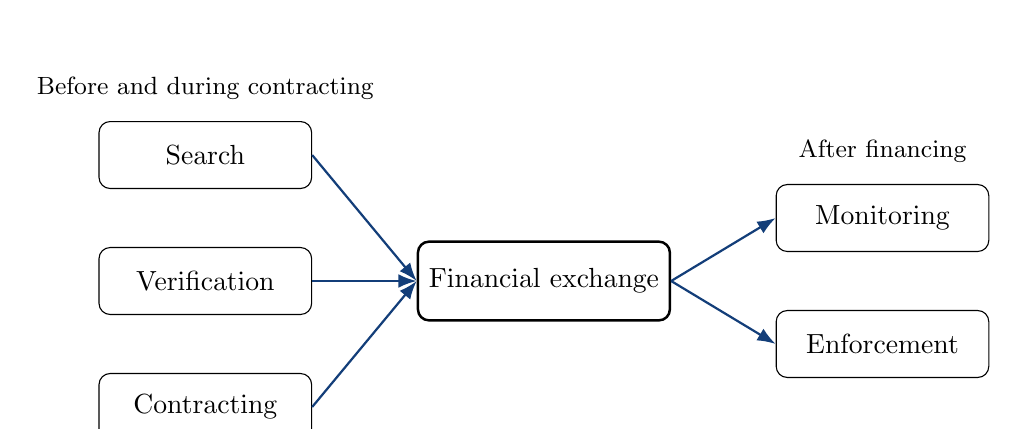
\begin{tikzpicture}[
    >=Latex,
    box/.style={
        draw,
        rounded corners,
        minimum width=2.7cm,
        minimum height=0.85cm,
        align=center
    },
    central/.style={
        draw,
        rounded corners,
        minimum width=3.2cm,
        minimum height=1.0cm,
        align=center,
        line width=0.9pt
    },
    flow/.style={
        -Latex,
        line width=0.8pt,
        FinanceBlue
    }
]

\node[central] (exchange) at (0,0) {Financial exchange};

\node[box] (search)   at (-4.3,1.6) {Search};
\node[box] (verify)   at (-4.3,0)   {Verification};
\node[box] (contract) at (-4.3,-1.6) {Contracting};

\node[box] (monitor) at (4.3,0.8) {Monitoring};
\node[box] (enforce) at (4.3,-0.8) {Enforcement};

\draw[flow] (search.east) -- (exchange.west);
\draw[flow] (verify.east) -- (exchange.west);
\draw[flow] (contract.east) -- (exchange.west);

\draw[flow] (exchange.east) -- (monitor.west);
\draw[flow] (exchange.east) -- (enforce.west);

\node[align=center] at (-4.3,2.45) {\small Before and during contracting};
\node[align=center] at (4.3,1.65) {\small After financing};

\end{tikzpicture}

\caption{Transaction costs around a financial relationship}
\label{fig:ch3-transaction-costs}
\end{figure}

Figure~\ref{fig:ch3-transaction-costs} presents a schematic representation rather than a strict chronological sequence. Verification may continue after a contract is signed, monitoring may generate new information, and the prospect of enforcement can influence behavior even before a breach occurs.

\subsection{Information Asymmetry and Costly Information Acquisition}

Information asymmetry exists when one party to a financial transaction has relevant information that the other does not. Some of this information may be obtainable, but acquiring and verifying it can be costly.

The asymmetry may concern characteristics. Borrowers may have better information about project quality than lenders, while managers may know more about expected cash flows than outside investors.

It may also concern actions. Lenders may be unable to observe fully how borrowers manage financed projects, while shareholders may not observe important managerial decisions after capital has been provided.

Asymmetric information is distinct from uncertainty. Future outcomes may remain uncertain even when all parties have access to the same information. The distinction lies in the distribution of information across parties, not in the existence of uncertainty itself.

Some information gaps can be reduced through additional information acquisition, but doing so requires resources. Let \(V(q)\) denote the economic value of information provided by a signal with precision \(q\), and let \(C(q)\) denote the cost of producing the signal.
Suppose the decision maker chooses information precision \(q\) to maximize net information value, \(V(q)-C(q)\). At a differentiable interior optimum, the marginal value of greater precision equals its marginal cost:

\begin{equation}
V'(q)=C'(q).
\label{eq:ch3-information-acquisition}
\end{equation}

Perfect information is not generally the objective. The relevant question is how much information is worth acquiring at a given cost. Banks, investors, and insurers therefore acquire information selectively, balancing its expected value against the resources required to obtain and process it.

Technological advances can change the economics of information acquisition by reducing the costs of collecting, processing, and evaluating information. Digital records, satellite data, electronic invoices, machine-learning methods, and automated document analysis can make previously costly information more accessible and easier to incorporate into financial decisions.

Lower information costs, however, do not necessarily improve information quality or decision value. Data may be biased, outdated, strategically manipulated, or only weakly related to the economic variable of interest. Efficient processing cannot compensate for signals with limited economic relevance.

\section{Adverse Selection: Hidden Information Before Contracting}

Adverse selection arises when privately known characteristics affect participation or contract choice \cite{Akerlof1970}. Different types respond differently to the terms offered, while the uninformed party cannot perfectly observe each participant's type before the contract is formed.

\subsection{Pooling Under Hidden Information} 

Suppose the applicant pool contains two borrower types, $H$ and $L$, with type $H$ associated with higher project quality than type $L$. The lender knows that a fraction $\pi$ of applicants are type $H$, but cannot observe the type of any individual applicant before contracting. In the absence of information that separates the two types, applicants are evaluated on a pooled basis.

If the lender assigns values $V_H$ and $V_L$ to the two types, with $V_H>V_L$, the pooled expected value of an unidentified applicant is

\begin{equation}
\bar V=\pi V_H+(1-\pi)V_L.
\label{eq:ch3-pooling-value}
\end{equation}

Under pooling, financing terms cannot be tailored to borrowers' privately known types. If participation decisions depend on the terms offered, higher-quality borrowers may be more likely to withdraw, reducing the average quality of the pool. The initial pooled valuation may then no longer reflect the composition of the borrowers who remain. This is the central mechanism of the \emph{lemons problem}.

The same mechanism appears across financial markets. When lenders cannot distinguish borrower quality, lower-risk borrowers may face interest rates that partly reflect the risk of higher-risk borrowers and may reduce their use of external finance. In insurance markets, pooled premiums may discourage low-risk customers while favoring the participation of high-risk customers. In securities markets, limited information about issuer quality may result in the undervaluation of higher-quality firms.

\subsection{Signaling by Informed Parties}

An informed party may convey private information through an observable signal \cite{Spence1973}. A signal is informative only when its cost or payoff consequences differ systematically across types.

Suppose a firm chooses a signal level $s$. The signaling cost for type $j$ is $c_j(s)$, where $j\in\{H,L\}$. A single-crossing condition can be written as

\begin{equation}
c_H'(s)<c_L'(s),
\label{eq:ch3-single-crossing}
\end{equation}
so that the marginal cost of signaling is lower for type $H$ than for type $L$. This difference can support a separating outcome in which the high-quality type chooses a signal that the low-quality type does not find worthwhile to imitate.

Financial signals may include retaining a larger equity stake, providing additional disclosure, accepting compensation tied more closely to performance, or committing assets or personal capital. Their informational content depends on differences in cost or commitment across types.

Statements that can be imitated at negligible cost convey little information. Costly commitments can be more credible when imitation is less attractive to lower-quality types.

Signaling can reduce informational distortions, but it is itself costly. Resources devoted to separating types may generate informational value without directly increasing project output.

\subsection{Screening by Uninformed Parties}

Screening occurs when the uninformed party designs contract terms that induce privately informed parties to reveal information through their choices. The mechanism works when different types prefer different contract options, allowing their choices to reveal their private information.

Suppose a lender offers two contracts. Contract $A$ carries a lower interest rate but requires more collateral, while contract $B$ requires less collateral but carries a higher interest rate. Different borrower types may value this trade-off differently. Their contract choices can therefore reveal information about type that the lender cannot observe directly.

A separating menu of contracts requires each type to prefer the contract intended for it. Let $C_H$ and $C_L$ denote the contracts intended for types $H$ and $L$, respectively. If $U_j(C_k)$ denotes the utility of type $j$ from contract $C_k$, where $j,k\in\{H,L\}$, incentive compatibility requires

\begin{equation}
\begin{aligned}
U_H(C_H) &\geq U_H(C_L),\\
U_L(C_L) &\geq U_L(C_H).
\end{aligned}
\label{eq:ch3-screening-ic}
\end{equation}

These conditions make self-selection consistent with type: type $H$ weakly prefers $C_H$, while type $L$ weakly prefers $C_L$. When the resulting choices differ across types, the lender can infer information about borrower type from the contract selected.

Contract-based screening takes different forms across financial markets. Lenders may vary collateral requirements or loan maturity, while insurers may vary deductibles or coverage limits.

When different types prefer similar contract terms, their choices reveal less information. Observable data can then supplement contract-based screening, with algorithmic credit scoring reducing the cost of information processing. However, predictive relationships may be unstable or vulnerable to strategic manipulation.

\subsection{Market Consequences: Mispricing, Credit Rationing, and Market Breakdown}

Under pooling, mispricing can arise when financing terms do not fully reflect differences in borrower quality. Higher-quality borrowers may face less favorable terms than under full information, while lower-quality borrowers may receive more favorable terms.

If these terms affect participation, some higher-quality borrowers may withdraw. The average quality of the remaining pool then declines, reinforcing the initial pricing problem. In more severe cases, mutually beneficial transactions may disappear and the market may partially or completely break down.

Credit rationing is a particularly important consequence in lending markets \cite{StiglitzWeiss1981}. In a standard competitive market, excess demand tends to put upward pressure on price. In credit markets with hidden borrower quality, however, a higher interest rate can also alter the composition of borrowers willing to borrow at that rate.

Normalize the loan principal to one and assume that the nonnegative project payoff is available to repay the lender, with no bankruptcy costs. Let \(\mathbb{E}_i\) denote expectation over borrowers willing to accept a loan at rate \(i\). The bank's expected repayment per unit lent is

\begin{equation}
\rho(i)=\mathbb{E}_i[\min\{1+i,X\}]
\label{eq:ch3-bank-return}
\end{equation}
where $X$ is the project payoff per unit borrowed. The bank receives $1+i$ when $X\geq 1+i$, and $X$ otherwise. A change in the lending rate affects both the contractual repayment
and the distribution of borrower types. 

The expected repayment $\rho(i)$ need not increase monotonically with the lending rate. Figure~\ref{fig:ch3-credit-rationing} illustrates one possible non-monotonic relationship. Its precise form depends on how borrower composition and project payoffs vary with the lending rate.

\begin{figure}[H]
\centering

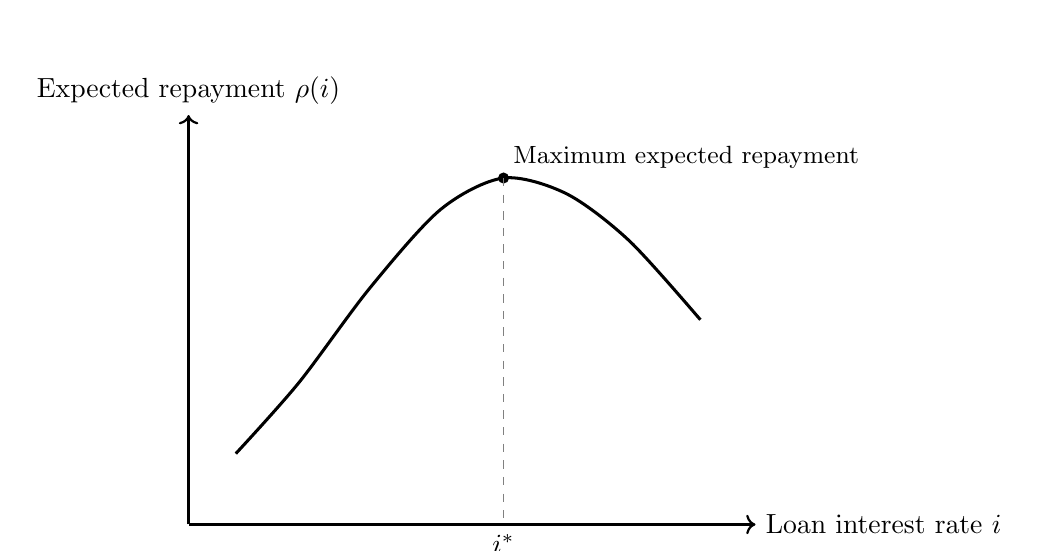
\begin{tikzpicture}[x=1cm,y=1cm]

% Axes
\draw[->, line width=0.8pt]
    (0,0) -- (7.2,0)
    node[right] {Loan interest rate $i$};

\draw[->, line width=0.8pt]
    (0,0) -- (0,5.2)
    node[above] { Expected repayment $\rho(i)$};

% Expected-return curve
\draw[line width=1.1pt, smooth]
    plot coordinates {
        (0.6,0.9)
        (1.4,1.8)
        (2.3,3.0)
        (3.2,4.0)
        (4.0,4.4)
        (4.8,4.2)
        (5.6,3.6)
        (6.5,2.6)
    };

% Maximum point
\fill (4.0,4.4) circle (2pt);

% Guide line
\draw[dashed, gray]
    (4.0,4.4) -- (4.0,0);

% Labels
\node[below] at (4.0,0) {$i^*$};
\node[above right] at (4.0,4.4)
    {\small Maximum expected repayment};

\end{tikzpicture}

\caption{An illustrative non-monotonic relationship
between the lending rate and expected repayment}
\label{fig:ch3-credit-rationing}
\end{figure}


In the illustrative case shown in Figure~\ref{fig:ch3-credit-rationing}, let $i^*$ denote the lending rate that maximizes expected repayment. If loan demand at $i^*$ exceeds the amount the bank is willing to lend, the bank may ration credit rather than raise the rate further, as doing so would reduce expected repayment.


\section{Moral Hazard: Hidden Actions After Contracting}

Unlike adverse selection, moral hazard concerns hidden actions after contracting. When those actions affect another party's payoff but cannot be fully observed or contracted upon, incentive problems can arise.

\subsection{Hidden Actions and Agency Problems}

Hidden action refers to an action chosen by the agent after contracting that affects the principal's payoff but cannot be fully observed or contracted upon. When the agent's incentives are not fully aligned with the principal's objective, this informational limitation gives rise to an agency problem.

Consider a principal who provides resources and an agent whose effort affects the outcome of a project. Let the project generate payoff $R$ if it succeeds and zero if it fails. The agent chooses effort $e$, which affects the probability of success $p(e)$ and entails private cost $c(e)$.

For simplicity, suppose both parties are risk-neutral, so monetary payoffs enter their objectives linearly. If the agent receives $w_S$ after success and $w_F$ after failure, expected utility is

\begin{equation}
U(e)=p(e)w_S+[1-p(e)]w_F-c(e).
\label{eq:ch3-agent-utility}
\end{equation}

The principal values effort for its contribution to project returns, while the agent considers contractual rewards and the private cost of effort. When effort is unobservable and the agent receives only part of the benefits it generates, the agent may choose less effort than would maximize the project's total surplus.

\subsection{Effort, Shirking, and Incentive Problems}

The efficient effort level $e^*$ maximizes
expected total surplus:

\begin{equation}
e^*\in\arg\max_e\left\{p(e)R-c(e)\right\}.
\label{eq:ch3-efficient-effort}
\end{equation}

If $e^*$ is an interior optimum, it satisfies

\begin{equation}
p'(e^*)R=c'(e^*).
\label{eq:ch3-efficient-effort-foc}
\end{equation}

The agent chooses effort to maximize the utility provided by the contract. Differentiating $U(e)$ with respect to effort, an interior optimum $\hat e$ satisfies

\begin{equation}
p'(\hat e)(w_S-w_F)=c'(\hat e).
\label{eq:ch3-agent-effort-foc}
\end{equation}

Comparing the two conditions identifies the source of the incentive problem. The project's marginal benefit from effort is $p'(e)R$, while the agent's private marginal benefit is $p'(e)(w_S-w_F)$. If $w_S-w_F<R$, the agent receives only part of the incremental value associated with greater effort. Under standard assumptions on $p(e)$ and $c(e)$, privately chosen effort may therefore fall below the efficient level. In this setting, the shortfall represents shirking.

\begin{example}{High and Low Effort}{high-low-effort}

Suppose the agent chooses between high effort $e_H$ and low effort $e_L$. High effort raises the probability of success but entails a higher private cost:

\begin{equation*}
p(e_H)>p(e_L),
\qquad
c(e_H)>c(e_L).
\end{equation*}

If the agent receives $w_S$ after success and $w_F$ after failure, high effort is preferred when

\begin{equation*}
p(e_H)w_S+[1-p(e_H)]w_F-c(e_H)
\geq
p(e_L)w_S+[1-p(e_L)]w_F-c(e_L).
\end{equation*}

Rearranging gives

\begin{equation*}
[p(e_H)-p(e_L)](w_S-w_F)
\geq
c(e_H)-c(e_L).
\label{eq:ch3-effort-spread}
\end{equation*}

The left-hand side is the additional expected compensation generated by the higher probability of success. The right-hand side is the additional private cost of high effort. A larger compensation differential between success and failure makes high effort more attractive relative to low effort.

\end{example}

Relaxing the risk-neutral assumption introduces an additional consideration. If the agent is risk-averse, greater sensitivity of compensation to outcomes strengthens incentives but also exposes the agent to more income risk when outcomes depend partly on factors outside the agent's control. Contract design may then involve a trade-off between incentive provision and risk sharing.

\subsection{Risk Shifting and Asset Substitution}

Post-contract incentive problems can arise through project choice as well as effort. After debt has been issued, equity holders may prefer a riskier project even when doing so reduces total firm value. This incentive is known as risk shifting. When a safer project or asset is replaced by a riskier one, the behavior is commonly described as asset substitution.

Under limited liability, equity holders receive the residual payoff after the promised debt repayment has been met, while their payoff is bounded below by zero.  If the firm's payoff is $X$ and promised debt repayment is $D$, the payoff to equity holders is

\begin{equation}
V_E(X)=\max\{X-D,0\}.
\label{eq:ch3-equity-payoff}
\end{equation}

This asymmetric payoff can make a riskier project attractive to equity holders even when it reduces total firm value.

\begin{example}{Risk Shifting after Debt Issuance}{risk-shifting-debt-issuance}

Suppose a firm has debt with face value \(D=80\). After the debt has been issued,
shareholders can choose between two projects. A safe project pays 110 with
certainty, leaving shareholders with \(110-80=30\).

A risky project pays 150 with probability \(0.5\) and 50 with probability \(0.5\).
Its expected total payoff is

\begin{equation*}
0.5(150)+0.5(50)=100,
\end{equation*}

which is lower than the safe project's payoff of 110. Under limited liability,
shareholders receive 70 in the high-payoff state and zero in the low-payoff state.
Their expected payoff is therefore

\begin{equation*}
0.5(70)+0.5(0)=35.
\label{eq:ch3-risk-shifting-example}
\end{equation*}

Shareholders therefore prefer the risky project even though it reduces total firm
value from 110 to 100. The expected repayment to creditors falls from 80 under the
safe project to

\begin{equation*}
0.5(80)+0.5(50)=65
\end{equation*}

under the risky project. The increase in shareholder value is accompanied by a
larger loss to creditors and a decline in total firm value.

\medskip

\begin{center}
\small
\textbf{Payoffs under the two project choices}

\medskip

\begin{tabularx}{\linewidth}{
  @{}
  >{\raggedright\arraybackslash}X
  >{\centering\arraybackslash}p{2.8cm}
  >{\centering\arraybackslash}p{3.0cm}
  @{}
}
\toprule
 & \textbf{Safe project} & \textbf{Risky project} \\
\midrule
Expected total payoff
    & 110 & 100 \\
Expected creditor repayment
    & 80 & 65 \\
Expected shareholder payoff
    & 30 & 35 \\
Firm-value ranking        & Higher & Lower \\
Shareholder payoff ranking & Lower & Higher \\
\bottomrule
\end{tabularx}
\end{center}

\end{example}


The possibility of post-financing risk shifting provides one rationale for contractual restrictions on changes in investment policy or business risk. Creditors are concerned not only with conditions at the time of lending, but also with decisions taken after financing has been provided.

\subsection{Private Benefits and Agency Costs}

Post-contract incentive conflicts can also arise when decision makers receive benefits that are not shared proportionally with outside investors. Managers may obtain private benefits through managerial perks, empire building, or projects that increase their control without increasing firm value. Controlling shareholders may similarly obtain benefits at the expense of minority investors.

Let a decision $a$ generate firm value $V(a)$ and private benefit $B(a)$ to the decision maker. If the decision maker owns a fraction $\alpha$ of the firm, the private payoff from the decision is

\begin{equation}
V_{\text{private}}(a)=\alpha V(a)+B(a).
\label{eq:ch3-private-benefits}
\end{equation}

When $\alpha<1$, the decision maker bears only a fraction of any reduction in firm value while retaining the private benefit. An action that maximizes private payoff may therefore differ from one that maximizes total firm value.

Private benefits can therefore generate a wedge between the action that maximizes the decision maker's private payoff and the action that maximizes firm value. This divergence gives rise to agency costs. Such costs include both resources devoted to limiting incentive conflicts and the residual loss that remains when those conflicts are not fully eliminated.

\section{Financial Contracts as Information and Incentive Solutions}

The information and incentive problems developed above create a role for contract design. Financial contracts do more than specify payments: they can influence participation, reveal private information, align incentives, and allocate rights when circumstances change.

These functions are often supported by disclosure, governance, auditing, reputation, and legal enforcement. Financial contracts therefore operate within a broader institutional framework.

\subsection{Collateral and Commitment}

Contract design can link repayment obligations to assets that remain available if the borrower fails to perform. Collateral provides such a link by giving the creditor a claim on specified assets. If the borrower defaults, the pledged assets provide a source of recovery for the creditor. Before default, the prospect of losing them can also affect the borrower's incentives.

If the amount owed is $D$  and the recoverable value of collateral is $C$, collateral-related loss can be expressed as

\begin{equation}
L=\max\{D-C,0\}.
\label{eq:ch3-collateral-loss}
\end{equation}

Collateral also affects borrower incentives before default. By exposing the borrower to the loss of pledged assets, it raises the private cost of actions that increase default risk. Collateral can therefore serve as both a recovery mechanism and a commitment device.

Collateral may also convey information when the cost of pledging assets differs across borrower types. Voluntary pledging can serve as a signal, while collateral requirements can induce self-selection across contracts. Its informational content therefore depends on whether different types face meaningfully different costs of providing collateral.

The effectiveness of collateral depends on the value and enforceability of the pledged assets. Collateral values can fall, while seizure and liquidation may be costly. Collateral requirements may also restrict financing for borrowers with valuable projects but limited pledgeable assets. Broad declines in collateral values can tighten borrowing constraints and amplify financial stress.

\subsection{Covenants and Control Rights}

Where collateral links repayment to specific assets, covenants govern borrower actions after financing has been provided. A covenant restricts or requires specified actions and may establish conditions that affect creditor rights.

Negative covenants may limit additional borrowing, asset sales, or distributions to shareholders. Affirmative covenants may require financial disclosure, preservation of collateral, or compliance with specified financial ratios.

Covenants focus on a limited set of observable or verifiable actions and financial conditions. When these terms are breached, the contract may trigger renegotiation or shift greater control to creditors, for example by requiring additional collateral, restricting distributions, or accelerating repayment.

Control rights are often state contingent. Managers retain greater discretion while contractual conditions are satisfied, whereas creditors gain influence when those conditions are breached.

\begin{figure}[H]
\centering
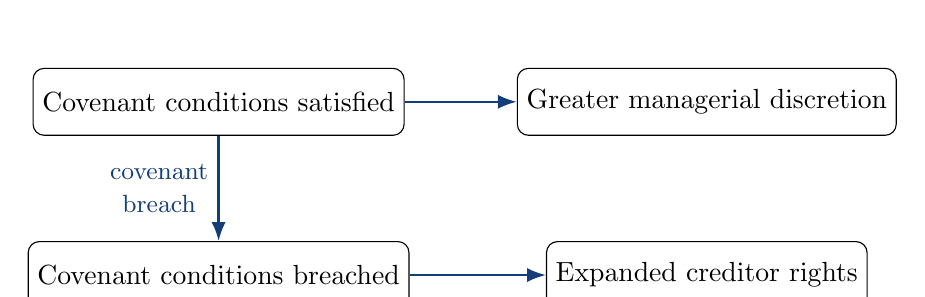
\begin{tikzpicture}[
  >=Latex,
  box/.style={
    draw,
    rounded corners,
    minimum width=3.5cm,
    minimum height=0.85cm,
    align=center
  },
  flow/.style={
    -Latex,
    line width=0.85pt,
    FinanceBlue
  }
]

\node[box] (satisfied) at (-1,2.2)
  {Covenant conditions satisfied};

\node[box] (manager) at (5.2,2.2)
  {Greater managerial discretion};

\node[box] (breach) at (-1,0)
  {Covenant conditions breached};

\node[box] (creditor) at (5.2,0)
  {Expanded creditor rights};

\draw[flow] (satisfied) -- (manager);
\draw[flow] (breach) -- (creditor);

\draw[flow] (satisfied) --
  node[left, align=center]{\small covenant\\\small breach}
  (breach);

\end{tikzpicture}

\caption{State-contingent allocation of control through covenants}
\label{fig:ch3-covenant-control}
\end{figure}

Financial covenants involve a trade-off between timely creditor intervention and unnecessary renegotiation. Overly restrictive thresholds may be breached following temporary fluctuations that do not indicate a material deterioration in the borrower's financial condition, while overly permissive thresholds may delay intervention until substantial value has been lost.

\subsection{Payoff Design and Incentive Compatibility}

Contract design can influence private choices by linking payoffs to observable outcomes or offering terms that encourage self-selection. Incentive compatibility requires each type to prefer its intended contract in screening and the intended action to be privately optimal when actions are hidden.

Equity retention, performance-contingent compensation, and insurance deductibles can strengthen incentives by increasing exposure to the consequences of individual decisions. However, greater payoff sensitivity may reduce risk sharing when outcomes also depend on factors beyond the agent's control. Contract design thus involves a trade-off between incentive provision and risk sharing.

\subsection{Monitoring and Information Production}

Monitoring produces and verifies information about borrower performance, compliance, and risk after financing has been provided. It can reveal potential violations and support the exercise of contractual rights. The prospect of detection and enforcement can also discourage actions that conflict with contractual obligations.

Monitoring may be underprovided when financial claims are widely dispersed. An individual claimant bears the cost of monitoring but shares the benefits with other claimants, creating a free-rider problem. Financial intermediaries can mitigate this problem by undertaking monitoring on behalf of multiple fund providers.

Technology can reduce monitoring costs through automated analysis of financial reports and transaction data. AI-assisted systems can identify potential irregularities, although their findings still require verification and economic interpretation.

\subsection{Governance and Enforcement}

Financial contracts operate within broader governance and enforcement arrangements. Governance concerns the allocation and exercise of decision and control rights among managers, boards, shareholders, creditors, and other parties. These rights may include approving major transactions, replacing managers, or intervening when specified conditions are met.

The allocation of rights alone does not ensure their effectiveness. Enforcement determines whether contractual and legal rights can be exercised in practice. Legal rules and institutions affect collateral recovery, acceleration of repayment, dispute resolution, and the enforcement of creditor priority in bankruptcy. They also provide remedies when managers or controlling shareholders breach their legal obligations.

Enforcement is not confined to court proceedings. Reputation can affect access to future transactions, while lenders and investors may withdraw future financing when commitments are violated. Exchanges and regulators can also impose continuing requirements and sanctions that reinforce compliance.

The expected effectiveness of enforcement also influences contract design. Where recovery is slow or uncertain, lenders may require more collateral, shorter maturities, tighter covenants, or higher credit spreads. Stronger governance and more reliable enforcement can make outside financing feasible with less direct intervention by investors. The same written contract may therefore have different economic value across institutional environments.

\begin{tcolorbox}[
  enhanced,
  breakable,
  colback=white,
  colframe=FinanceBlue,
  boxrule=0.7pt,
  sharp corners,
  borderline west={2.2pt}{0pt}{FinanceBlue},
  title=\textbf{Financial Perspective: Information Alone Does Not Solve the Contracting Problem},
  coltitle=white,
  colbacktitle=FinanceBlue,
  fonttitle=\bfseries,
  before skip=1.2em,
  after skip=1.2em
]

Better information can improve financial decisions without eliminating incentive or enforcement problems. A lender may assess default risk accurately while remaining unable to control the borrower's actions after financing. Detailed disclosure can improve shareholder information without giving outside investors effective control over managerial decisions. An AI model may identify deteriorating credit quality, but the value of that information still depends on the rights and remedies available in response. Information, incentives, and enforceable rights are therefore complements rather than substitutes.

\end{tcolorbox}

%========================================================
% Summary
%========================================================

\TailModule{summary}{Summary}

Financial transactions require information about counterparties, projects, and future behavior. Producing and verifying this information is costly, and relevant information is often distributed asymmetrically across parties.

Adverse selection arises from hidden information before a contract is formed. When quality cannot be observed directly, pooled pricing can discourage higher-quality participants from entering or remaining in the market, reducing the average quality of the remaining pool and, in severe cases, contributing to market breakdown. Signaling allows informed parties to reveal type when signals are differentially costly to imitate, while screening uses contract choices to induce self-selection. In credit markets, higher lending rates can worsen borrower composition, so a bank's expected repayment need not increase monotonically with the lending rate. Credit rationing can therefore arise even when some borrowers are willing to borrow at higher rates.

Moral hazard arises from hidden actions after contracting \cite{Holmstrom1979,JensenMeckling1976}. Shirking, risk shifting, and the pursuit of private benefits can cause privately optimal actions to differ from those preferred by lenders, investors, or insurers. Financial contracts respond by altering payoffs, commitments, and control rights. Collateral, covenants, equity retention, deductibles, monitoring, and state-contingent control can improve incentives, while governance and enforcement determine how rights are exercised in practice.

These mechanisms involve trade-offs. Stronger incentives can reduce risk sharing, tighter contractual restrictions can limit valuable flexibility, collateral requirements can constrain borrowers with few pledgeable assets, and monitoring is costly. Contract design therefore seeks to reduce information and incentive problems at reasonable economic cost rather than eliminate them completely.

%========================================================
% Mind Map
%========================================================

\TailModule{mindmap}{Mind Map}
\begin{figure}[H]
\centering
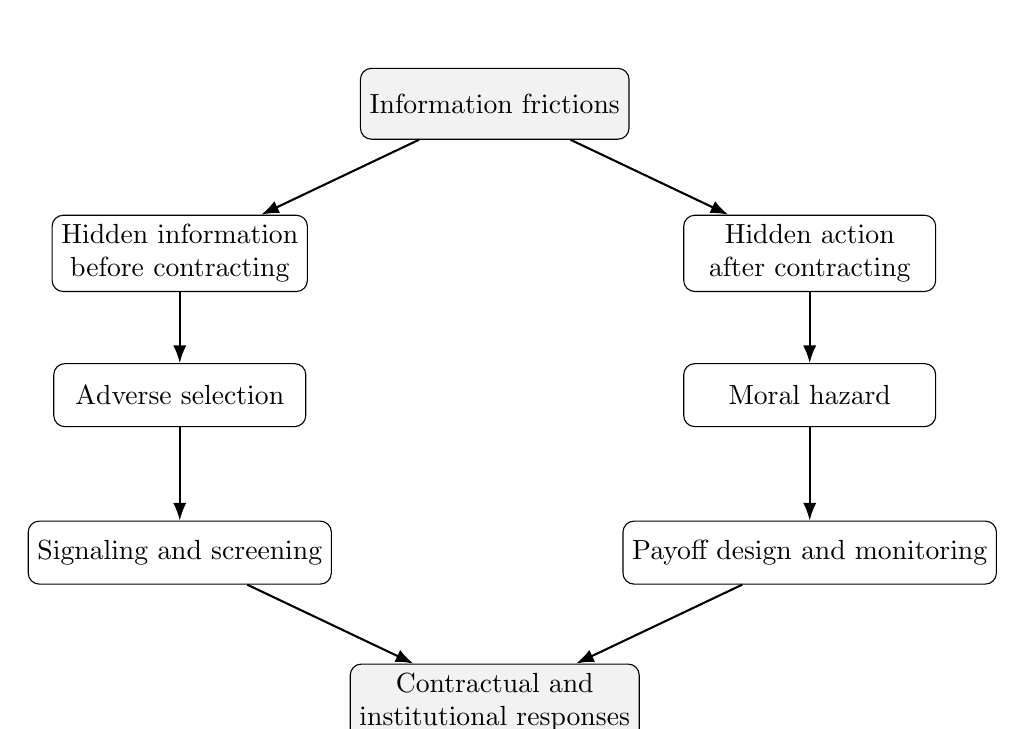
\begin{tikzpicture}[
  >=Latex,
  main/.style={
    draw,
    rounded corners,
    minimum width=3.4cm,
    minimum height=0.9cm,
    align=center,
    fill=gray!10
  },
  sub/.style={
    draw,
    rounded corners,
    minimum width=3.2cm,
    minimum height=0.8cm,
    align=center
  },
  flow/.style={-Latex, line width=0.75pt}
]

\node[main] (friction) at (0,4.2)
  {Information frictions};

\node[sub] (hiddeninfo) at (-4.0,2.3)
  {Hidden information\\before contracting};

\node[sub] (hiddenaction) at (4.0,2.3)
  {Hidden action\\after contracting};

\node[sub] (adverse) at (-4.0,0.5)
  {Adverse selection};

\node[sub] (moral) at (4.0,0.5)
  {Moral hazard};

\node[sub] (responses1) at (-4.0,-1.5)
  {Signaling and screening};

\node[sub] (responses2) at (4.0,-1.5)
  {Payoff design and monitoring};

\node[main] (responses) at (0,-3.4)
  {Contractual and\\institutional responses};

\draw[flow] (friction) -- (hiddeninfo);
\draw[flow] (friction) -- (hiddenaction);
\draw[flow] (hiddeninfo) -- (adverse);
\draw[flow] (hiddenaction) -- (moral);
\draw[flow] (adverse) -- (responses1);
\draw[flow] (moral) -- (responses2);
\draw[flow] (responses1) -- (responses);
\draw[flow] (responses2) -- (responses);

\end{tikzpicture}

\caption*{Information problems before and after contracting}
\end{figure}

%========================================================
% Key Terms
%========================================================

\TailModule{keyterms}{Key Terms}

Transaction costs; information asymmetry; costly information acquisition; hidden information; adverse selection; pooling; signaling; screening; incentive compatibility; credit rationing; hidden action; moral hazard; principal--agent problem; risk shifting; asset substitution; private benefits; agency costs; collateral; covenant; control rights; monitoring; governance; enforcement


%========================================================
% Financial AI Lab
%========================================================

\TailModule{aiprompt}{Financial AI Lab}

\textbf{Lab: Design and Audit an AI Credit-Screening Framework}

Ask an AI system to propose a credit-screening framework for a small-business lender. Require it to identify observable variables and explain how each variable may be related to repayment risk. Separate information available before lending from information that would become available only after financing, and explain why the latter belongs to monitoring rather than initial screening.

Then audit the proposed framework. Which variables contain information about underlying borrower quality, which are only correlated with it, and which could be manipulated once applicants understand the screening rule? Identify one potential source of selection bias, one fairness concern, and one reason a model trained on past borrowers might perform poorly when credit conditions change.

Finally, suppose the model predicts default risk with high accuracy. Explain which problems would still require contractual terms, collateral, monitoring, enforcement, or human review. Why does accurate prediction not by itself eliminate the contracting problem?

%========================================================
% Discussion Questions
%========================================================

\TailModule{questions}{Discussion Questions}

\begin{enumerate}

\item Why is uncertainty not the same as asymmetric information? Give a financial example in which uncertainty is high but information is symmetric, and another in which information is asymmetric.

\item Why can a higher lending rate reduce a bank's expected
repayment per unit lent even as the promised repayment increases?

\item Compare signaling and screening. Who takes the initiative in each case, and what allows different types to be distinguished?

\item Why does improved information about borrower behavior
after financing not necessarily eliminate moral hazard?
Explain the roles of monitoring, contractual incentives,
control rights, and enforcement.
\end{enumerate}

%========================================================
% Applied Problems
%========================================================

\TailModule{appprobs}{Applied Problems}

\begin{enumerate}

\item An investor considers purchasing claims on firms' future project cash flows. The investor believes that 70\% of the claims are high-quality, with value 120 to the investor, and 30\% are low-quality, with value 60. The investor cannot observe the quality of an individual claim
    \begin{enumerate}

    \item Calculate the pooled expected value.
    
    \item Suppose high-quality firms are willing to sell only at a price of at least 110, while low-quality firms are willing to sell at a price of at least 55. If the investor initially offers the pooled expected value, which types accept the offer, and how does the composition of claims offered for sale change?

    \item Explain the adverse-selection mechanism in economic terms.

    \end{enumerate}

\item An agent chooses between high and low effort. High effort produces success with probability $0.8$ and has a private cost of 12. Low effort produces success with probability $0.5$ and has a private cost of 3. The agent receives $w_S$ after success and zero after failure.

  \begin{enumerate}

  \item Derive the incentive-compatibility condition for high effort and determine the threshold value of $w_S$.

  \item Explain why increasing the success-contingent payment affects the agent's effort choice.

  \item What additional trade-off arises if the agent is risk-averse?

  \end{enumerate}

\item A firm has debt with face value 80. Shareholders can choose between Project A, which pays 112 with certainty, and Project B, which pays 160 with probability $0.5$ and 48 with probability $0.5$.

  \begin{enumerate}

  \item Calculate the expected total payoff of each project.

  \item Calculate the expected shareholder payoff under each project.

  \item Does the project preferred by shareholders maximize total firm value? Explain the source of the conflict.

  \end{enumerate}

\end{enumerate}

%========================================================
% Case Analysis
%========================================================

\TailModule{caseanalysis}{Case Analysis}

\textbf{Luckin Coffee: When Reported Information Cannot Be Taken at Face Value}

In December 2020, the U.S. Securities and Exchange Commission charged Luckin Coffee Inc. with defrauding investors by materially misstating its revenue, expenses, and net operating loss. According to the SEC complaint, from at least April 2019 through January 2020, Luckin intentionally fabricated more than US\$300 million in retail sales. The company agreed to a settlement, subject to court approval, that included a US\$180 million civil penalty, without admitting or denying the SEC's allegations.\footnote{U.S. Securities and Exchange Commission, ``Luckin Coffee Agrees to Pay \$180 Million Penalty to Settle Accounting Fraud Charges,'' Press Release 2020-319, December 16, 2020.}

Use the SEC's December 16, 2020 enforcement release and related company disclosures as primary sources. Analyze the episode through the framework of this chapter. What information did outside investors rely on? Which information-production and verification mechanisms were intended to reduce the information asymmetry between insiders and outside investors? What does the episode reveal about both the value and the limits of external audit as a verification mechanism? Which monitoring, governance, internal-control, and enforcement mechanisms became important once the reported information was challenged? Finally, distinguish between an \emph{information failure} and an \emph{incentive or governance failure} in the case.

\emph{Primary source: U.S. Securities and Exchange Commission, ``Luckin Coffee Agrees to Pay \$180 Million Penalty to Settle Accounting Fraud Charges,'' Press Release 2020-319, December 16, 2020.}
%========================================================
% Further Reading
%========================================================

\TailModule{furtherread}{Further Reading}

\begin{itemize}

\item Akerlof, George A. (1970), ``The Market for `Lemons': Quality Uncertainty and the Market Mechanism,'' \emph{The Quarterly Journal of Economics}, 84(3), 488--500.

\item Spence, Michael (1973), ``Job Market Signaling,'' \emph{The Quarterly Journal of Economics}, 87(3), 355--374.

\item Jensen, Michael C., and William H. Meckling (1976), ``Theory of the Firm: Managerial Behavior, Agency Costs and Ownership Structure,'' \emph{Journal of Financial Economics}, 3(4), 305--360.

\item Stiglitz, Joseph E., and Andrew Weiss (1981), ``Credit Rationing in Markets with Imperfect Information,'' \emph{American Economic Review}, 71(3), 393--410.

\item Diamond, Douglas W. (1984), ``Financial Intermediation and Delegated Monitoring,'' \emph{The Review of Economic Studies}, 51(3), 393--414.

\end{itemize}
\ChapterTail{summary,mindmap,keyterms,aiprompt,questions,appprobs,caseanalysis,furtherread}

\chapter{Financial Intermediation and Financial Structure}
\label{chap:Financial_Intermediation_and_Financial_Structure}

\begin{openingcase}{Why Does a Large Firm Issue Bonds While a Small Firm Borrows from a Bank?}

Two manufacturers need external financing. A large listed firm plans to raise RMB 2 billion through a bond issue, while a small private firm seeking RMB 5 million turns to a bank. The contrast seems puzzling: issuing bonds allows firms to obtain funds directly from investors rather than borrowing through a bank. Why would the smaller firm rely on an intermediary?

The listed firm has audited financial statements and a large financing need over which to spread issuance costs. For the smaller firm, information about its customers, equipment, and management is difficult for outside investors to verify. A bank with an existing relationship may be better positioned to assess and monitor the borrower.

Intermediation adds another institution to the financing process, yet it may reduce the overall cost of obtaining and maintaining financing.

\end{openingcase}


\begin{tcolorbox}[
  enhanced,
  colback=FinanceBlue!6,
  colframe=FinanceBlue,
  boxrule=0.6pt,
  sharp corners,
  left=8pt,
  right=8pt,
  top=7pt,
  bottom=7pt,
  before skip=1em,
  after skip=1.6em,
  title=\textbf{Core Questions},
  coltitle=white,
  colbacktitle=FinanceBlue,
  fonttitle=\bfseries,
  attach boxed title to top left={xshift=6pt,yshift=-2mm},
  boxed title style={
    boxrule=0pt,
    sharp corners,
    left=5pt,
    right=5pt,
    top=2pt,
    bottom=2pt
  }
]
\begin{enumerate}[
  leftmargin=*,
  label=\textcolor{FinanceBlue}{\textbf{\arabic*.}},
  itemsep=0.55em,
  topsep=0.2em
]
\item What determines whether financing is organized through securities markets or through financial intermediaries?

\item Why can delegated information production, monitoring, and balance-sheet transformation create value?

\item Why do markets and intermediaries coexist, and what determines their relative importance in a financial system?

\end{enumerate}
\end{tcolorbox}

\section{Financing Channels: Direct and Indirect Finance}

A financing channel is defined by the claims that connect ultimate fund providers with ultimate users. In direct finance, fund providers hold claims issued by the ultimate borrower. In indirect finance, an intermediary acquires the borrower's claim and finances it by issuing claims of its own. The presence of other institutions does not change this distinction; what matters is whether an intermediary inserts its balance sheet between the two sides.

\begin{figure}[htbp]
\centering

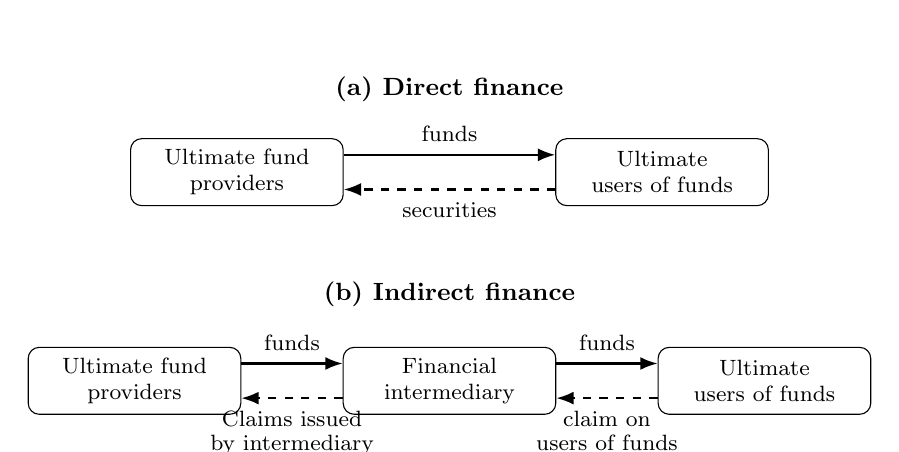
\begin{tikzpicture}[
    box/.style={
        draw,
        rounded corners,
        align=center,
        minimum width=2.7cm,
        minimum height=0.85cm,
        inner sep=3pt
    },
    fund/.style={
        -{Latex[length=2.2mm]},
        thick
    },
    claim/.style={
        -{Latex[length=2.2mm]},
        dashed,
        thick
    },
    every node/.style={font=\footnotesize}
]

% ------------------------------------------------
% (a) Direct finance
% ------------------------------------------------

\node[font=\small\bfseries] at (0,1.05)
    {(a) Direct finance};

\node[box] (providersA) at (-2.7,0)
    {Ultimate fund\\providers};

\node[box] (borrowerA) at (2.7,0)
    {Ultimate\\users of funds};

\draw[fund]
    ([yshift=2.2mm]providersA.east)
    --
    node[above=1pt]{funds}
    ([yshift=2.2mm]borrowerA.west);

\draw[claim]
    ([yshift=-2.2mm]borrowerA.west)
    --
    node[below=1pt]{securities}
    ([yshift=-2.2mm]providersA.east);


% ------------------------------------------------
% (b) Indirect finance
% ------------------------------------------------

\node[font=\small\bfseries] at (0,-1.55)
    {(b) Indirect finance};

\node[box] (providersB) at (-4.0,-2.65)
    {Ultimate fund\\providers};

\node[box] (intermediary) at (0,-2.65)
    {Financial\\intermediary};

\node[box] (borrowerB) at (4.0,-2.65)
    {Ultimate\\users of funds};

\draw[fund]
    ([yshift=2.2mm]providersB.east)
    --
    node[above=1pt]{funds}
    ([yshift=2.2mm]intermediary.west);

\draw[claim]
    ([yshift=-2.2mm]intermediary.west)
    --
    node[below=1pt, align=center]
    {Claims issued \\[-1pt] by intermediary}
    ([yshift=-2.2mm]providersB.east);

\draw[fund]
    ([yshift=2.2mm]intermediary.east)
    --
    node[above=1pt]{funds}
    ([yshift=2.2mm]borrowerB.west);

\draw[claim]
    ([yshift=-2.2mm]borrowerB.west)
    --
    node[below=1pt, align=center]
    {claim on\\[-1pt]users of funds}
    ([yshift=-2.2mm]intermediary.east);

\end{tikzpicture}

\caption{Direct and indirect financing channels.}
\label{fig:ch4-direct-indirect-finance}
\end{figure}

\subsection{Direct Finance and Securities Markets}

The distinction between direct and indirect finance rests on the structure of financial claims connecting ultimate fund providers with users of funds. In direct finance, fund providers hold claims issued by the users of funds. In indirect finance, an intermediary holds claims on these users and finances them by issuing its own financial claims. The distinction rests on whether an intermediary interposes its own balance sheet between fund providers and users.

Direct finance does not imply the absence of financial institutions. Investment banks may arrange or underwrite an issue, rating agencies may assess credit risk, and exchanges or dealers may facilitate trading. These institutions support the financing process, but they do not insert their own balance sheets between the issuer and investors.

For securities to be distributed among many investors, claims need to be sufficiently standardized and relevant information needs to be communicated and verified in forms that a broad investor base can use. Payment rights, maturity, collateral, seniority, and voting rights are specified in common contractual terms, while audited financial statements, disclosure requirements, prospectuses, and ratings provide widely accessible information. These arrangements reduce the need for investors to investigate the issuer and negotiate contract terms separately.

A securities issue entails fixed costs that can be spread over a larger financing amount. Suppose the total transaction cost of an issue of size $Q$ is

\begin{equation}
C_M(Q)=F_M+c_MQ,
\label{eq:ch4-market-financing-cost}
\end{equation}
where $F_M$ represents fixed costs associated with disclosure, legal work, due diligence, registration, and issue organization, and $c_M$ is the variable transaction cost per unit of financing. The average transaction cost is

\begin{equation}
AC_M(Q)=\frac{F_M}{Q}+c_M,
\label{eq:ch4-market-average-cost}
\end{equation}
so that
\begin{equation}
\frac{dAC_M(Q)}{dQ}
=-\frac{F_M}{Q^2}
<0.
\label{eq:ch4-market-scale-effect}
\end{equation}

As issue size increases, fixed costs are spread over a larger financing base, lowering average transaction cost and making market financing more economical.

Information costs also influence the choice of financing channel. When an issuer's financial condition and cash flows can be credibly disclosed and verified, dispersed investors can evaluate its securities at relatively low cost, making market financing more attractive.  

A secondary market allows investors to sell securities without requiring the issuer to repay or renegotiate the financing. Tradability therefore separates the issuer's financing horizon from the holding periods of individual investors. This benefit depends on market liquidity, which in turn requires active trading, reliable information, and supporting market infrastructure and may deteriorate sharply under stress.

\subsection{Indirect Finance and Financial Intermediaries}

In indirect finance, a financial intermediary provides funds to borrowers and holds the resulting claims, financing those assets by issuing its own liabilities to fund providers.

Commercial banks illustrate this structure. Depositors hold claims on the bank, while the bank holds claims on the firms and households to which it lends. A simplified balance sheet makes this two-sided structure explicit.
 
\begin{table}[htbp]

\centering

\caption{A Simplified Balance Sheet of a Commercial Bank}

\label{tab:ch4-bank-balance-sheet}

\begin{tabularx}{0.78\textwidth}{@{}X X@{}}

\toprule

\textbf{Assets} & \textbf{Liabilities and Equity} \\

\midrule

Loans                      & Deposits \\
Securities                 & Wholesale funding \\
Reserves and liquid assets & Equity capital \\

\bottomrule

\end{tabularx}

\end{table}

The intermediary therefore interposes its own balance sheet between fund providers and borrowers. It holds a claim on the borrower, typically a loan, while fund providers hold claims issued by the intermediary. The intermediary assesses creditworthiness, negotiates loan terms, and monitors borrower performance.

This arrangement concentrates information production within the intermediary. Through repeated lending and direct contact with borrowers, a bank can accumulate information that would be costly for dispersed investors to produce separately. Much of this information can remain private, allowing the intermediary to evaluate borrowers without relying entirely on standardized public disclosure.

The same arrangement also delegates substantial decision-making authority to the intermediary, creating a new agency relationship. Fund providers do not normally observe individual lending or risk-management decisions. The intermediary's ability to meet its obligations therefore depends in part on the quality of its lending decisions, liquidity management, and risk control. Capital, governance, reputation, supervision, and regulation help constrain this delegated discretion and sustain confidence in the intermediary's liabilities.

Intermediation can improve financing efficiency when the benefits of specialized information production and monitoring outweigh the agency costs of delegated decision-making, particularly when borrower information is difficult to standardize or verify publicly.

\subsection{Financing Chains and Hybrid Intermediation}

A financing chain links ultimate fund providers to ultimate users through a sequence of financial claims. Hybrid intermediation arises when securities markets and financial intermediaries perform different functions at different stages of that chain.

\begin{figure}[htbp]
\centering

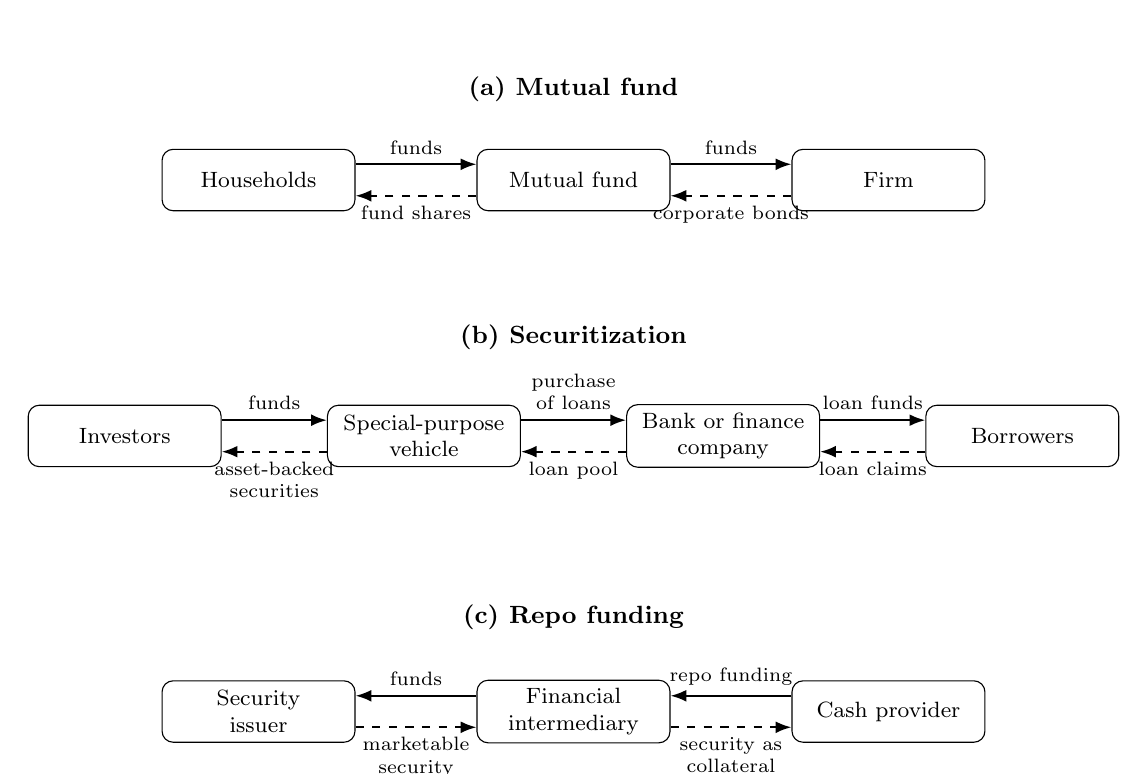
\begin{tikzpicture}[
    box/.style={
        draw,
        rounded corners,
        align=center,
        minimum width=2.45cm,
        minimum height=0.78cm,
        inner sep=3pt,
        font=\footnotesize
    },
    fund/.style={
        -{Latex[length=2.0mm]},
        line width=0.75pt
    },
    claim/.style={
        -{Latex[length=2.0mm]},
        dashed,
        line width=0.75pt
    },
    labeltext/.style={
        font=\scriptsize,
        align=center
    },
    panel/.style={
        font=\small\bfseries
    }
]

% ==================================================
% (a) Mutual fund
% ==================================================

\node[panel] at (0,1.15)
    {(a) Mutual fund};

\node[box] (hh) at (-4.0,0)
    {Households};

\node[box] (mf) at (0,0)
    {Mutual fund};

\node[box] (firm) at (4.0,0)
    {Firm};

% funds
\draw[fund]
    ([yshift=2mm]hh.east)
    --
    node[above, labeltext]{funds}
    ([yshift=2mm]mf.west);

\draw[fund]
    ([yshift=2mm]mf.east)
    --
    node[above, labeltext]{funds}
    ([yshift=2mm]firm.west);

% claims
\draw[claim]
    ([yshift=-2mm]mf.west)
    --
    node[below, labeltext]{fund shares}
    ([yshift=-2mm]hh.east);

\draw[claim]
    ([yshift=-2mm]firm.west)
    --
    node[below, labeltext]{corporate bonds}
    ([yshift=-2mm]mf.east);


% ==================================================
% (b) Securitization
% ==================================================

\node[panel] at (0,-2.0)
    {(b) Securitization};

\node[box] (investors) at (-5.7,-3.25)
    {Investors};

\node[box] (spv) at (-1.9,-3.25)
    {Special-purpose\\vehicle};

\node[box] (originator) at (1.9,-3.25)
    {Bank or finance\\company};

\node[box] (borrowers) at (5.7,-3.25)
    {Borrowers};

% funds
\draw[fund]
    ([yshift=2mm]investors.east)
    --
    node[above, labeltext]{funds}
    ([yshift=2mm]spv.west);

\draw[fund]
    ([yshift=2mm]spv.east)
    --
    node[above, labeltext]{purchase\\of loans}
    ([yshift=2mm]originator.west);

\draw[fund]
    ([yshift=2mm]originator.east)
    --
    node[above, labeltext]{loan funds}
    ([yshift=2mm]borrowers.west);

% claims
\draw[claim]
    ([yshift=-2mm]borrowers.west)
    --
    node[below, labeltext]{loan claims}
    ([yshift=-2mm]originator.east);

\draw[claim]
    ([yshift=-2mm]originator.west)
    --
    node[below, labeltext]{loan pool}
    ([yshift=-2mm]spv.east);

\draw[claim]
    ([yshift=-2mm]spv.west)
    --
    node[below, labeltext]{asset-backed\\securities}
    ([yshift=-2mm]investors.east);


% ==================================================
% (c) Repo funding
% ==================================================
\node[panel] at (0,-5.55)
    {(c) Repo funding};
\node[box] (issuer) at (-4.0,-6.75)
    {Security\\issuer};

\node[box] (fi) at (0,-6.75)
    {Financial\\intermediary};

\node[box] (cash) at (4.0,-6.75)
    {Cash provider};

% Intermediary purchases security
\draw[fund]
    ([yshift=2mm]fi.west)
    --
    node[above, labeltext]{funds}
    ([yshift=2mm]issuer.east);

\draw[claim]
    ([yshift=-2mm]issuer.east)
    --
    node[below, labeltext]{marketable\\security}
    ([yshift=-2mm]fi.west);

% Repo funding
\draw[fund]
    ([yshift=2mm]cash.west)
    --
    node[above, labeltext]{repo funding}
    ([yshift=2mm]fi.east);

\draw[claim]
    ([yshift=-2mm]fi.east)
    --
    node[below, labeltext]{security as\\collateral}
    ([yshift=-2mm]cash.west);

\end{tikzpicture}

\caption{Examples of hybrid financing chains.}
\label{fig:ch4-hybrid-financing}
\end{figure}

A corporate bond held by a mutual fund provides a simple example. The corporation raises funds by issuing a marketable security, while household investors hold fund shares rather than the corporation's bonds directly. The issuer uses market financing, while household savings reach the market through an intermediary.

Securitization extends the chain by separating loan origination and screening from the subsequent distribution of funding and risk. A bank or finance company originates and screens loans, pools them, and transfers them to a special-purpose vehicle, which issues securities backed by the loan cash flows. Information production remains concentrated near origination, while funding and risk bearing can be distributed through securities markets.

Marketable securities can also support intermediary funding. In a repo transaction, a financial institution obtains short-term funding against securities that it agrees to repurchase later. Securities held on intermediary balance sheets can therefore become collateral for money-market funding, linking securities markets to intermediary funding.

Markets and intermediaries are therefore often complementary. The useful distinction is not whether an entire financing chain is market based or intermediated, but where information is produced, how funding is obtained, where liquidity is provided, and who ultimately bears risk.

\section{Why Do Financial Intermediaries Exist?}

Financial intermediation adds an organizational layer to financing but may reduce the costs of information production, contracting, monitoring, and trading through specialization and scale. These benefits must be weighed against the costs of intermediation.

\subsection{Transaction Costs, Scale, and Specialization}

Repeated transactions allow financial intermediaries to spread the costs of information systems, standardized procedures, and monitoring infrastructure across many borrowers. Experience with similar transactions can also improve their ability to assess and manage risk.

One source of this advantage is that some costs do not increase proportionately with transaction volume. Suppose an activity has a fixed cost component $F$ and a variable cost $c$ per transaction. Its average cost over $n$ transactions is

\begin{equation}
AC(n)=\frac{F}{n}+c.
\label{eq:ch4-scale-cost}
\end{equation}

As $n$ increases, the fixed cost per transaction declines. Scale also supports specialization: expertise in credit analysis, contracting, risk management, and transaction processing can be employed across many transactions rather than reproduced by individual investors. Standardized procedures can generate further savings when similar tasks are performed repeatedly.

Lower transaction costs can make otherwise uneconomical financing viable. Suppose financing a small business generates an expected surplus of $S$ before information and contracting costs. If an individual investor incurs costs $k>S$, direct financing is uneconomical. An intermediary may make the transaction viable if its total cost of providing these services is below $S$.

The gains from scale are not unlimited. As an intermediary grows, additional organizational layers can weaken internal incentives, increase procedural rigidity, and reduce the effective use of local or relationship-specific information. Organizational costs may therefore rise even as some transaction costs fall.

\subsection{Information Production and Delegated Monitoring}

Financial intermediaries produce information by collecting, verifying, and interpreting borrower-specific data. Before financing, this information supports screening and the setting of financing terms. After financing, monitoring updates the intermediary's assessment of the borrower and detects changes in behavior or credit quality. When financing is dispersed across many investors, concentrating these activities within an intermediary can avoid repeated information production.

Consider monitoring after financing. Suppose $N$ investors finance the same borrower and each incurs monitoring cost $m$ if monitoring is performed separately. Total monitoring cost is

\begin{equation}
C_D=Nm.
\label{eq:ch4-direct-monitoring}
\end{equation}

Monitoring can instead be delegated to a financial intermediary. Let $m_I$ denote the intermediary's monitoring cost and $g$ the agency cost created by delegation. Total cost under delegated monitoring is

\begin{equation}
C_I=m_I+g.
\label{eq:ch4-delegated-monitoring}
\end{equation}

Delegated monitoring lowers total cost when

\begin{equation}
m_I+g<Nm.
\label{eq:ch4-delegation-condition}
\end{equation}

The term $g$ captures the new agency problem created by delegation. Fund providers cannot fully observe the intermediary's monitoring effort or risk-taking decisions. The intermediary may therefore monitor borrowers less carefully or take more risk than fund providers would prefer.

The size of $g$ depends on the incentives and constraints facing the intermediary. Equity capital exposes shareholders to losses from poor lending decisions or excessive risk taking. Audited financial reporting improves the information available to creditors, investors, and supervisors about the intermediary's asset quality, capital position, and risk exposure. Contractual restrictions and prudential regulation can further limit risk taking that shifts potential losses toward fund providers. These mechanisms can reduce, but not eliminate, the agency cost of delegation.

\subsection{Private Information and Relationship Lending}

Repeated interaction allows lenders to accumulate private information from repayment behavior, account activity, collateral conditions, and direct contact with management. Some of this information is difficult to quantify, codify, or communicate to outside investors and is often described as \emph{soft information}. It may include assessments of managerial competence and the persistence of financial difficulties.

Relationship lending uses information accumulated through ongoing lender–borrower relationships to assess borrowers whose creditworthiness is difficult to evaluate from standardized disclosures. Such information may allow lenders to distinguish between firms that appear similar to outside investors, improving access to finance for borrowers with limited public information.

The informational advantage also matters after financing has been provided. When a borrower experiences a temporary setback, a relationship lender may be better able to distinguish a short-term cash-flow shock from a deterioration in underlying creditworthiness and determine whether continued lending or renegotiation is warranted.

Private information can also create borrower dependence. Information accumulated by one lender may not be readily transferable to competitors, increasing switching costs and strengthening the incumbent lender's bargaining power. Relationship lending thus involves a trade-off between improved credit assessment and the potential costs of borrower dependence and lender market power.

\subsection{Liquidity, Maturity, and Risk Transformation}

In addition to producing information, financial intermediaries transform the characteristics of financial claims. Liquidity transformation arises when fund providers value access to funds on short notice while borrowers require financing for long-lived, illiquid assets. A bank bridges this mismatch by issuing liquid deposits while holding less liquid loans.

Pooling idiosyncratic liquidity needs across many depositors reduces uncertainty in aggregate withdrawals. The timing of liquidity needs is uncertain for any individual depositor, but aggregate withdrawals become more predictable when those needs are not perfectly correlated. A simple model illustrates this mechanism.

Suppose there are $N$ depositors. Each has probability $\lambda$ of needing one unit of liquidity during the period. If liquidity needs are independent, the expected number of depositors requiring funds is

\begin{equation}
\mathbb{E}[L]=N\lambda.
\label{eq:ch4-liquidity-expected}
\end{equation}

The variance is

\begin{equation}
\mathrm{Var}(L)=N\lambda(1-\lambda).
\label{eq:ch4-liquidity-variance}
\end{equation}

The standard deviation grows with $\sqrt{N}$, while expected liquidity needs grow with $N$, so relative uncertainty declines as $N$ increases:

\begin{equation}
\frac{\sqrt{\mathrm{Var}(L)}}{\mathbb{E}[L]}
=
\sqrt{\frac{1-\lambda}{N\lambda}}.
\label{eq:ch4-liquidity-relative-risk}
\end{equation}

Lower relative uncertainty in aggregate withdrawals allows an intermediary to hold more long-term, less liquid assets while still providing liquid claims to depositors.

When withdrawals become highly correlated, a liquidity mismatch can expose an intermediary to severe funding pressure. The intermediary may need to obtain additional funding or sell illiquid assets to meet withdrawal demands.

Liquidity transformation is often accompanied by maturity transformation. A bank can fund long-term loans with shorter-maturity liabilities, allowing borrowers to obtain long-term finance while fund providers hold shorter-term claims. The resulting maturity mismatch exposes the bank to refinancing risk, as maturing liabilities may need to be rolled over before sufficient cash flows are received from its assets.

Alongside liquidity and maturity transformation, financial intermediaries also engage in risk transformation through diversification and the allocation of losses. By combining loans with imperfectly correlated credit risks, a bank can reduce its exposure to borrower-specific risk. Its capital structure also determines how losses are allocated across financial claims, with equity absorbing losses before creditors.

\begin{table}[htbp]
\centering
\caption{Financial Transformation through Intermediaries}
\label{tab:ch4-transformation}

\renewcommand{\arraystretch}{1.15}

\begin{tabularx}{\textwidth}{
@{}
>{\raggedright\arraybackslash}p{3.2cm}
>{\raggedright\arraybackslash}X
>{\raggedright\arraybackslash}X
@{}
}

\toprule
\textbf{Transformation}
& \textbf{Assets or exposures}
& \textbf{Claims issued to fund providers} \\
\midrule

Liquidity transformation
& Relatively illiquid assets
& More liquid or readily redeemable claims \\

Maturity transformation
& Longer-maturity assets
& Shorter-maturity liabilities \\

Risk transformation
& Diversified loan portfolio
& Equity and debt claims with different loss exposures \\

\bottomrule
\end{tabularx}

\end{table}



\section{Financial Structure: Markets, Banks, and Hybrid Systems}

Financial structure describes how financing is organized through financial markets, intermediaries, and combinations of the two.

\subsection{Market-Based versus Bank-Based Financial Systems}

Financial systems differ in the relative importance of securities markets and banks in channeling funds to users of finance. The distinction is one of degree rather than a strict division between two types of systems.

Market-based finance relies more heavily on standardized disclosure, transferable financial claims, and market prices. These arrangements facilitate financing by dispersed investors when relevant information can be evaluated at relatively low cost. Contractual rights and governance mechanisms provide additional means of investor oversight.

Bank-based finance relies more heavily on private information and continuing borrower relationships. Concentrated monitoring and adaptable loan contracts can be advantageous when borrower information is difficult to verify publicly or financing requires ongoing adjustment.

The relative costs of market and bank financing depend on firm characteristics and financial-system conditions. Larger financing amounts allow fixed issuance costs to be spread more widely, while credible public disclosure reduces information costs for dispersed investors. Bank financing may be more economical when borrower assessment requires private information, continuing monitoring, or renegotiation. Securities-market depth and liquidity, together with banks' funding and regulatory constraints, also influence the relative costs of the two channels.

At the system level, the composition of firms influences the relative importance of market and bank financing. Economies with more large and transparent firms may rely more heavily on securities markets, while bank finance may play a greater role where borrower-specific information and continuing monitoring are important. Legal institutions, disclosure standards, market infrastructure, and financial regulation also influence the development of the two channels.

\begin{table}[htbp]
\centering
\caption{Market-Based and Bank-Based Financing}
\label{tab:ch4-market-bank}

\renewcommand{\arraystretch}{1.15}

\begin{tabularx}{\textwidth}{
@{}
>{\raggedright\arraybackslash}p{3.0cm}
>{\raggedright\arraybackslash}X
>{\raggedright\arraybackslash}X
@{}
}

\toprule
& \textbf{Market financing}
& \textbf{Bank financing} \\
\midrule

Information
& Greater reliance on standardized public information
& Greater use of privately produced borrower information \\

Monitoring
& Investor oversight through disclosure, governance, and delegated monitoring
& Concentrated within a specialized intermediary \\

Contracting
& More standardized and transferable claims
& Greater scope for customized contracts \\

Liquidity for fund providers
& Through secondary-market trading
& Through liquid bank liabilities, such as deposits \\

Renegotiation
& More difficult when claims are widely dispersed
& Often easier within a continuing lending relationship \\

Conditions favoring the channel
& Large financing needs and greater public transparency
& Greater opacity and stronger need for monitoring or renegotiation \\

\bottomrule
\end{tabularx}
\end{table}

\subsection{Hybrid and Platform-Based Financial Systems}

Hybrid financial systems combine market-based and intermediary-based mechanisms within interconnected financing chains. Household savings may reach securities markets through investment funds, while bank-originated loans may be transferred to investors through securitization.

Digital platforms can separate financial functions traditionally combined within a single intermediary. A lending platform may collect borrower data, verify applications, assess creditworthiness, standardize contracts, and service repayments, while the resulting claims may be retained by the platform, transferred to banks, or sold to institutional investors. When claims are transferred while servicing remains with the platform, information processing and loan servicing become separated from funding and risk bearing.

\begin{tcolorbox}[
  enhanced,
  breakable,
  colback=white,
  colframe=FinanceBlue,
  boxrule=0.7pt,
  sharp corners,
  borderline west={2.2pt}{0pt}{FinanceBlue},
  title={Financial Perspective: Financial Functions and Institutional Forms},
  coltitle=white,
  colbacktitle=FinanceBlue,
  fonttitle=\bfseries,
  before skip=1.2em,
  after skip=1.2em
]

Institutional labels do not necessarily identify the
economic functions an organization performs.
A platform that arranges and services loans while
transferring the resulting claims has different
risk exposures from one that retains the loans.
The relevant distinctions concern who provides
funding, holds financial claims, exercises control,
and bears losses.

\end{tcolorbox}

\begin{example}{China's Hybrid Financial Structure}
{china-hybrid-financial-structure}

China's financial system combines substantial bank
intermediation with bond and equity markets.
The People's Bank of China's Aggregate Financing
to the Real Economy framework records financing
through bank loans, corporate bonds, equity issuance,
and other channels. Credit-asset securitization
further connects banking and securities markets
by allowing bank-originated loans to be transferred
to structures that issue securities to investors.

\end{example}

\section{What Shapes Financial Structure?}

\subsection{Legal Institutions and Investor Protection}

Legal institutions influence financial structure through the protection and enforcement of financial claims. For creditors, bankruptcy procedures, priority rules, and collateral rights affect expected recovery. For outside shareholders, legal and governance protections can limit the diversion of corporate resources and protect their rights in corporate decision-making.

These protections are particularly important in securities markets, where dispersed investors have limited scope for individual negotiation and monitoring. Standardized disclosure, investor rights, and effective enforcement can support financing through a broad investor base.

Bank financing relies more heavily on borrower-specific contracts and concentrated monitoring, but also depends on enforceable creditor rights. Weak or uncertain enforcement can reduce expected recovery and restrict credit supply.

Investor protection also influences ownership and control structures. Stronger protection of outside shareholders can support dispersed ownership, while weaker protection may encourage concentrated ownership and monitoring by large shareholders. Concentrated control, however, may also allow controlling shareholders to extract private benefits at the expense of minority investors.

\subsection{Economic Development and Financial Deepening}

Economic development can affect financial structure by increasing the demand for financial services and making a wider range of financial arrangements economically viable. Growth in income, wealth, and economic activity can expand the scale of financial activity. Larger transaction volumes can, in turn, spread the fixed costs of information production, financial infrastructure, and securities issuance over a broader base.

Financial deepening refers to an increase in the scale and range of financial intermediation and market activity relative to the size of the economy. It can occur through the expansion of bank credit, securities markets, institutional investors, and financial infrastructure. These components can reinforce one another. Growth of institutional investors can increase demand for marketable securities, while well-developed government bond markets can provide benchmark yields for pricing other securities and collateral for financial transactions.

\begin{figure}[htbp]
\centering

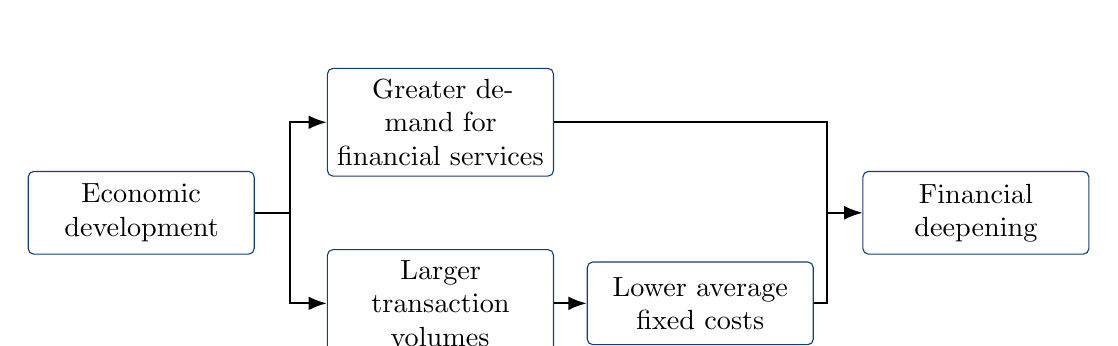
\begin{tikzpicture}[
    >=Latex,
    box/.style={
        draw=FinanceBlue,
        rounded corners=2pt,
        align=center,
        minimum height=1.05cm,
        text width=2.8cm,
        inner xsep=1pt,
        inner ysep=4pt
    },
    arrow/.style={
        -Latex,
        line width=0.8pt
    }
]

% Nodes
\node[box] (development) at (0,0)
{Economic development};

\node[box] (demand) at (3.8,1.15)
{Greater demand for\\financial services};

\node[box] (volume) at (3.8,-1.15)
{Larger transaction\\volumes};

\node[box] (cost) at (7.1,-1.15)
{Lower average\\fixed costs};

\node[box] (deepening) at (10.6,0)
{Financial deepening};

% Arrows
\draw[arrow] (development.east) -- ++(0.45,0) |- (demand.west);
\draw[arrow] (development.east) -- ++(0.45,0) |- (volume.west);

\draw[arrow] (demand.east) -| ([xshift=-0.45cm]deepening.west) -- (deepening.west);
\draw[arrow] (volume.east) -- (cost.west);
\draw[arrow] (cost.east) -| ([xshift=-0.45cm]deepening.west) -- (deepening.west);

\end{tikzpicture}

\caption{Economic development and financial deepening}
\label{fig:ch4-financial-deepening}
\end{figure}

Economic development can support both financial intermediaries and securities markets. As financial systems deepen, the two can become increasingly interconnected through funding, investment, and liquidity relationships.

Financial depth, however, is not equivalent to financial efficiency. An increase in credit, market capitalization, or financial assets does not by itself imply more efficient resource allocation. Credit may expand toward projects with low expected returns, leverage may increase financial fragility, and securities markets may grow without corresponding improvements in disclosure or enforcement. The economic value of financial deepening depends on whether the expansion of finance improves capital allocation, information production, risk sharing, liquidity, and access relative to the costs and vulnerabilities it introduces.

\subsection{Technology and Financial Infrastructure}

Technological advances can influence financial structure by reducing the costs of information processing and financial transactions. Digital information systems may lower screening and verification costs, while electronic trading systems can reduce securities transaction costs.

These effects need not be symmetric across markets and intermediaries. When technology lowers the cost of standardizing and publicly verifying borrower information, market finance may become more feasible for borrowers that are difficult for dispersed investors to assess. By contrast, when proprietary transaction data improve screening and monitoring, banks or platforms with extensive data may gain a relative informational advantage.

Financial infrastructure provides another channel through which technology influences financial structure. Markets and intermediaries depend on systems that record claims, transfer funds, exchange information, and settle transactions. The reliability and interoperability of these systems can affect the efficiency of different financing channels.


\subsection{Regulation and Institutional Change}

Regulation can affect financial structure by changing the costs and constraints associated with different financial arrangements. Capital, liquidity, disclosure, and investment rules can alter the conditions under which banks, securities issuers, and institutional investors operate, even when their primary objectives are prudential regulation or investor protection.

Differences in regulatory treatment can affect how financial activities are organized. If regulation raises the cost of holding a particular credit exposure on a bank balance sheet, part of that activity may shift toward securities markets or nonbank intermediaries. The underlying function of credit provision may remain similar even as the institutional form changes. Such shifts can reallocate rather than eliminate risk, as market-based and nonbank arrangements may involve different combinations of leverage, funding structures, and liquidity risk.

Regulation also interacts with financial innovation. New financing arrangements may prompt regulatory responses, which in turn influence their viability and organization.

%========================================================
% Summary
%========================================================

\TailModule{summary}{Summary}

Financial structure concerns how financing, information production, monitoring, liquidity provision, and risk allocation are organized across markets and intermediaries. In direct finance, investors hold claims issued by the ultimate users of funds. In indirect finance, an intermediary holds claims on borrowers and issues its own financial claims to fund providers. Modern financial systems commonly combine both forms within interconnected financing chains.

Market finance becomes more effective when information can be standardized and publicly evaluated and when financing scale spreads fixed issuance costs. Intermediaries can create value through specialization, economies of scale, private information production, and delegated monitoring. Delegation can reduce duplicated monitoring by dispersed investors but introduces an agency problem between fund providers and the intermediary.

Intermediaries also transform the characteristics of financial claims. Pooling liquidity needs can support liquid liabilities backed by less liquid assets, while maturity transformation permits longer-term assets to be financed with shorter-term liabilities. Risk transformation operates through pooling and the allocation of losses across financial claims. These transformations provide financial services while also creating potential sources of fragility.

The relative roles of markets and intermediaries depend on both the characteristics of financing and the broader economic and institutional environment. Legal protection and enforcement, economic development, technology, financial infrastructure, and regulation can alter the costs and feasibility of alternative financial arrangements. Financial structure evolves as markets, intermediaries, and hybrid arrangements adapt to changing economic and institutional conditions.

%========================================================
% Mind Map
%========================================================

\TailModule{mindmap}{Mind Map}

\begin{figure}[H]
\centering

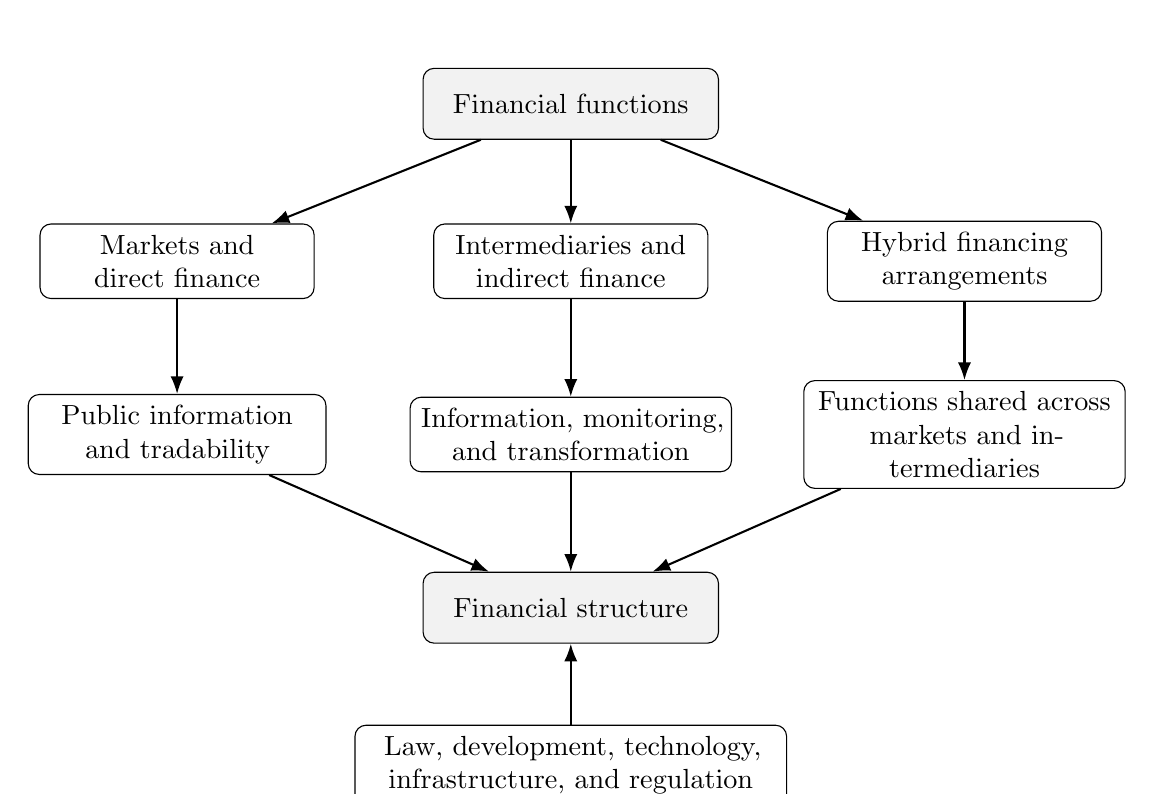
\begin{tikzpicture}[
  >=Latex,
  main/.style={
    draw,
    rounded corners,
    minimum height=0.9cm,
    align=center,
    fill=gray!10,
    inner xsep=5pt,
    inner ysep=4pt
  },
  sub/.style={
    draw,
    rounded corners,
    minimum height=0.85cm,
    align=center,
    inner xsep=4pt,
    inner ysep=4pt
  },
  flow/.style={
    -Latex,
    line width=0.75pt
  }
]

% Top
\node[main, text width=3.4cm] (functions) at (0,4.2)
{Financial functions};

% Organizational forms
\node[sub, text width=3.2cm] (markets) at (-5.0,2.2)
{Markets and\\direct finance};

\node[sub, text width=3.2cm] (inter) at (0,2.2)
{Intermediaries and\\indirect finance};

\node[sub, text width=3.2cm] (hybrid) at (5.0,2.2)
{Hybrid financing\\arrangements};

% Mechanisms
\node[sub, text width=3.5cm] (marketmech) at (-5.0,0)
{Public information\\and tradability};

\node[sub, text width=3.8cm] (intermech) at (0,0)
{Information, monitoring,\\and transformation};

\node[sub, text width=3.8cm] (hybridmech) at (5.0,0)
{Functions shared across\\markets and intermediaries};

% Financial structure
\node[main, text width=3.4cm] (structure) at (0,-2.2)
{Financial structure};

% Environment
\node[sub, text width=5.2cm] (environment) at (0,-4.2)
{Law, development, technology,\\infrastructure, and regulation};

% Arrows
\draw[flow] (functions) -- (markets);
\draw[flow] (functions) -- (inter);
\draw[flow] (functions) -- (hybrid);

\draw[flow] (markets) -- (marketmech);
\draw[flow] (inter) -- (intermech);
\draw[flow] (hybrid) -- (hybridmech);

\draw[flow] (marketmech) -- (structure);
\draw[flow] (intermech) -- (structure);
\draw[flow] (hybridmech) -- (structure);

\draw[flow] (environment) -- (structure);

\end{tikzpicture}

\caption*{From financial functions to financial structure}
\end{figure}

%========================================================
% Key Terms
%========================================================

\TailModule{keyterms}{Key Terms}

Direct finance; indirect finance; financial intermediary; financing chain; hybrid financial system; economies of scale; delegated monitoring; relationship lending; liquidity pooling; liquidity transformation; maturity transformation; risk transformation; financial structure; market-based financial system; bank-based financial system; financial deepening; investor protection; financial infrastructure; platform-based finance; non-bank financial intermediation

%========================================================
% Financial AI Lab
%========================================================

\TailModule{aiprompt}{Financial AI Lab}

\textbf{Lab: Reconstruct the Financing Chain}

Choose a contemporary financing arrangement, such as a digital lending platform, private credit fund, securitization vehicle, crowdfunding platform, or online wealth-management product. Ask an AI system to classify the arrangement as direct or indirect finance, and treat its initial classification as provisional.

Reconstruct the full financing chain. Identify the ultimate supplier and user of funds, the financial claims created at each stage, and the party that holds each claim. Then determine who performs screening and monitoring, who provides liquidity, and who ultimately bears credit losses.

Compare your reconstruction with the AI classification. If market and intermediary functions are combined within the same financing chain, explain why a simple direct--indirect classification may be insufficient. Verify the institutional structure and allocation of risk using primary documents from the relevant financial institution, regulator, exchange, or platform.

%========================================================
% Discussion Questions
%========================================================

\TailModule{questions}{Discussion Questions}

\begin{enumerate}

\item Why does the involvement of an investment bank in a corporate bond issue not necessarily make the transaction indirect finance?

\item Explain the delegated-monitoring argument for financial intermediation. How can delegation reduce duplicated monitoring while creating a new agency problem?

\item How does an increase in the number of depositors reduce the relative uncertainty of aggregate liquidity needs when individual liquidity needs are not perfectly correlated?

\item Why is the distinction between market-based and bank-based financial systems better understood as a matter of degree rather than a binary classification?

\item How can the same technological change affect securities markets and financial intermediaries differently?

\end{enumerate}

%========================================================
% Data Application
%========================================================

\TailModule{dataapp}{Data Application}

\textbf{Financial Structure in China and International Comparison}

Use the IMF Financial Development Index database to compare the Financial Institutions Index and the Financial Markets Index for China and at least three other economies over a common period. Choose economies with meaningfully different financial structures and examine whether financial development has occurred primarily through institutions, markets, or both. Interpret the indices as measures of different dimensions of financial development rather than as rankings of superior and inferior financial systems.

For China, use the People's Bank of China's Aggregate Financing to the Real Economy statistics to examine the composition of financing. Compare RMB loans with selected direct-financing categories, such as corporate bonds and domestic equity financing by non-financial corporations. Explain why financing flows measured by AFRE and the IMF indices capture different dimensions of financial structure.

Use the evidence to evaluate one proposition from this chapter, such as the continuing importance of bank intermediation, the development of market-based finance, or the coexistence of both channels. Report the indicator definitions, sample period, economies selected, and primary data sources.

%========================================================
% Further Reading
%========================================================

\TailModule{furtherread}{Further Reading}

\begin{itemize}

\item Diamond, Douglas W. (1984), ``Financial Intermediation and Delegated Monitoring,'' 
\emph{The Review of Economic Studies}, 51(3), 393--414.

\item Allen, Franklin, and Douglas Gale (2000), 
\emph{Comparing Financial Systems}, MIT Press.

\item Levine, Ross (2002), ``Bank-Based or Market-Based Financial Systems: Which Is Better?'' 
\emph{Journal of Financial Intermediation}, 11(4), 398--428.

\item Beck, Thorsten, Asli Demirg\"{u}\c{c}-Kunt, and Ross Levine (2003), 
``Law and Finance: Why Does Legal Origin Matter?'' 
\emph{Journal of Comparative Economics}, 31(4), 653--675.

\item Svirydzenka, Katsiaryna (2016), 
``Introducing a New Broad-based Index of Financial Development,'' 
IMF Working Paper No.~16/5.

\end{itemize}

\ChapterTail{summary,mindmap,keyterms,aiprompt,questions,dataapp,furtherread}
\chapter{The Logic of Financial Valuation}
\label{chap:The_Logic_of_Financial_Valuation}

\begin{openingcase}{The Same Expected Cash Flow, but the Same Value?}

An investor is comparing two one-year financial claims. Each has an expected payoff of RMB 100. Claim A pays RMB 120 when the economy is strong and RMB 80 when it is weak. Claim B does the opposite: it pays RMB 80 in the strong economy and RMB 120 in the weak economy. Suppose the two states are equally likely.

Their expected payoffs are identical:

\[
0.5(120)+0.5(80)=100.
\]

Yet the two claims need not have the same current value. Claim B pays more when economic conditions are weak, when an additional unit of cash may be particularly valuable. The distribution of payoffs across economic states can therefore affect valuation even when expected payoffs are identical.

\end{openingcase}

\begin{tcolorbox}[
  enhanced,
  colback=FinanceBlue!6,
  colframe=FinanceBlue,
  boxrule=0.6pt,
  sharp corners,
  left=8pt,
  right=8pt,
  top=7pt,
  bottom=7pt,
  before skip=1em,
  after skip=1.6em,
  title=\textbf{Core Questions},
  coltitle=white,
  colbacktitle=FinanceBlue,
  fonttitle=\bfseries,
  attach boxed title to top left={xshift=6pt,yshift=-2mm},
  boxed title style={
    boxrule=0pt,
    sharp corners,
    left=5pt,
    right=5pt,
    top=2pt,
    bottom=2pt
  }
]
\begin{enumerate}[
  leftmargin=*,
  label=\textcolor{FinanceBlue}{\textbf{\arabic*.}},
  itemsep=0.55em,
  topsep=0.2em
]

\item Why is expected cash flow alone insufficient to determine the value of a financial claim?

\item How do the timing, risk, and state dependence of future cash flows affect their present value?

\item How do information, contractual rights, and market prices interact in determining the value of financial claims?

\end{enumerate}
\end{tcolorbox}


\section{The Foundations of Financial Value}

A financial claim derives its value from the future economic benefits to which it entitles the holder. Before applying a valuation formula, three questions need to be addressed:


\begin{itemize}[
  leftmargin=2.2em,
  itemsep=0.45em,
  topsep=0.55em
]

\item What cash flows does the claim entitle its holder to receive?

\item When are these cash flows received?

\item How do these cash flows vary across future states of the world?

\end{itemize}

\subsection{Financial Assets as Claims on Future Economic Resources}

A financial asset represents rights to future economic resources, typically expressed through future cash flows.
A bond gives the holder contractual rights to specified payments, while common stock gives the holder a residual claim on the corporation after more senior claims have been satisfied. A derivative creates contingent cash flows that depend on an underlying asset, rate, index, or state variable.

The object of valuation is therefore the \emph{claim} defined by these rights, rather than simply the issuer, project, or underlying asset. Suppose a firm's operating assets generate cash flow $Y_t$ at date $t$. This cash flow may be allocated among several claimants:

\begin{equation}
Y_t=C_{D,t}+C_{E,t}+C_{O,t},
\label{eq:ch5-cash-flow-allocation}
\end{equation}
where $C_{D,t}$ denotes cash flow to debt holders, $C_{E,t}$ cash flow to equity holders, and $C_{O,t}$ cash flow to other contractual claimants.

The value of a financial claim depends not only on the cash flow generated by the underlying assets, but also on the contractual rules that determine how that cash flow is allocated.

Priority provides a simple illustration. Consider a firm financed only by debt and equity. Suppose it generates cash flow $Y$ in the next period and has debt with a promised repayment of $D$. Abstracting from other contractual provisions, debt holders receive

\begin{equation}
C_D=\min\{Y,D\},
\label{eq:ch5-debt-payoff}
\end{equation}
while equity holders receive

\begin{equation}
C_E=\max\{Y-D,0\}.
\label{eq:ch5-equity-payoff}
\end{equation}

Thus,

\begin{equation*}
C_D+C_E=Y.
\label{eq:ch5-claim-additivity}
\end{equation*}

The contractual structure does not change the firm's total cash flow; it determines how that cash flow is allocated across claimants for each realization of \(Y\). Figure~\ref{fig:ch5-debt-equity-payoff} illustrates this allocation.

\begin{figure}[H]

\centering

\begin{tikzpicture}[
=Latex,
axis/.style={-Latex, line width=0.8pt},
debt/.style={line width=1.0pt, FinanceBlue},
equity/.style={line width=1.0pt, dashed}
 ]

\draw[axis] (0,0) -- (7.2,0) node[right] {Firm cash flow $Y$};
\draw[axis] (0,0) -- (0,5.4) node[above] {Claim cash flow};

\draw[debt] (0,0) -- (3.6,3.6) -- (6.6,3.6);
\draw[equity] (0,0) -- (3.6,0) -- (6.6,3.0);

\draw[dashed, gray] (3.6,0) -- (3.6,4.6);

\node[below] at (3.6,0) {$D$};
\node[FinanceBlue, right] at (6.0,3.85) {Debt};
\node[right] at (6.2,2.55) {Equity};

\end{tikzpicture}
\caption{Allocation of firm cash flow between debt and equity}
\label{fig:ch5-debt-equity-payoff}

\end{figure}

\subsection{Time and the Present Value of Future Cash Flows}

A cash flow received in the future is not generally equivalent in value to an equal cash flow received today. Individuals may require compensation for postponing current consumption; funds available today can also be invested to generate future returns. These considerations provide the basic economic foundation for the time value of money and for interest and discounting.

A future cash flow can be expressed in terms of an equivalent amount today by discounting it at an appropriate rate.

Let \(V_0\) denote the present value of a claim that pays a certain cash flow \(CF_1\) one period from now. If the relevant one-period risk-free rate is \(r_{f}\), no-arbitrage equivalence requires:

\begin{equation*}
V_0(1+r_{f})=CF_1.
\label{eq:ch5-one-period-equivalence}
\end{equation*}
which gives

\begin{equation*}
V_0=\frac{CF_1}{1+r_{f}}.
\label{eq:ch5-one-period-pv}
\end{equation*}

The factor $1/(1+r_{f})$ is the one-period discount factor.
It gives the present value of one unit of cash flow
received one period in the future.

Assuming a constant per-period discount rate $r$,
the present value of a cash flow $CF_t$ received
$t$ periods from now is

\[
V_0=\frac{CF_t}{(1+r)^t}.
\]

For a sequence of future cash flows, the present
value is

\begin{equation}
V_0=\sum_{t=1}^{T}
\frac{CF_t}{(1+r)^t}.
\label{eq:ch5-pv-cash-flow-stream}
\end{equation}

Discounting expresses cash flows occurring at different dates in terms of value at a common date. Once expressed on this common basis, the cash flows can be compared and added.

\begin{figure}[H]
\centering
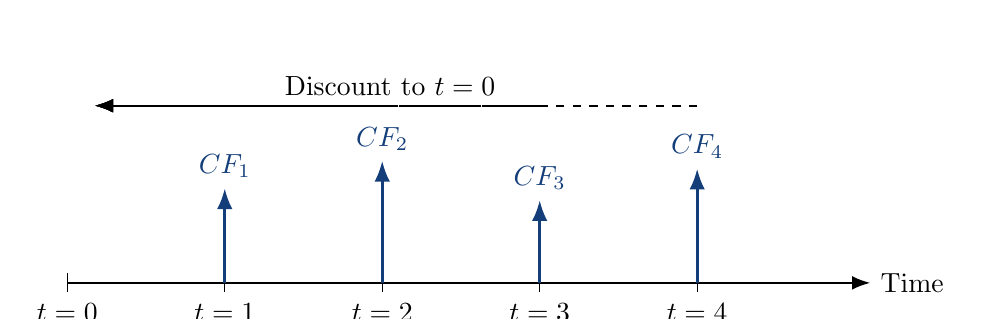
\begin{tikzpicture}[
  >=Latex,
  axis/.style={-Latex, line width=0.8pt},
  cash/.style={-Latex, line width=1.0pt, FinanceBlue},
  discount/.style={-Latex, dashed, line width=0.8pt}
]

\draw[axis] (0,0) -- (10.2,0) node[right]{Time};

\foreach \x/\t in {0/0,2/1,4/2,6/3,8/4}
{
  \draw (\x,0.12) -- (\x,-0.12);
  \node[below=4pt] at (\x,0) {$t=\t$};
}

\draw[cash] (2,0) -- (2,1.2) node[above] {$CF_1$};
\draw[cash] (4,0) -- (4,1.55) node[above] {$CF_2$};
\draw[cash] (6,0) -- (6,1.05) node[above] {$CF_3$};
\draw[cash] (8,0) -- (8,1.45) node[above] {$CF_4$};

\draw[discount] (2,2.25) -- (0.35,2.25);
\draw[discount] (4,2.25) -- (0.35,2.25);
\draw[discount] (6,2.25) -- (0.35,2.25);
\draw[discount] (8,2.25) -- (0.35,2.25);

\node[above] at (4.1,2.25) {Discount to $t=0$};

\end{tikzpicture}

\caption{Discounting future cash flows to the present}
\label{fig:ch5-discount-timeline}
\end{figure}

Several implications follow directly from discounting.

First, timing matters even when total nominal cash flow is unchanged. If two claims make the same total payments but one pays earlier, the earlier payments generally have greater present value when discount rates are positive.

Second, the sensitivity of present value to the discount rate increases with the time to payment. A change in the discount rate therefore has a larger effect on more distant cash flows.

Third, the timing of cash flows must be consistent with the discount-rate convention. An annual rate cannot be applied directly to quarterly cash flows without an appropriate conversion, and cash flows occurring at the beginning of a period must be distinguished from those occurring at the end.

\begin{example}{Timing Alone Changes Value}{timing-alone-changes-value}

Suppose Claim A pays RMB~1,000 one year from now and Claim B pays RMB~1,000 five years from now. If the relevant annual rate is 5 \%,

\[
V_A=\frac{1,000}{1.05}=952.38,
\]

while

\[
V_B=\frac{1,000}{1.05^5}=783.53.
\]

The nominal future payment is identical. The present value differs only because the payment dates differ.

\end{example}

\subsection{Risk and Required Return}

Time alone does not determine value. Many financial claims have risky future cash flows. Suppose there are two possible states next period. A claim pays $CF_H$ in one state and $CF_L$ in the other, with probabilities $p$ and $1-p$, respectively. Its expected cash flow is

\begin{equation}
\mathrm{E}[X]=pCF_H+(1-p)CF_L.
\label{eq:ch5-expected-cash-flow}
\end{equation}

Expected cash flow alone is generally insufficient for valuation. The value of a claim also depends on the risk of its cash flows. Cash flows that tend to be low when overall economic conditions are poor expose investors to greater risk. Such claims generally require a higher expected return. Two claims with the same expected payoff may consequently have different current values.

One common way to incorporate risk into valuation is through a required return. Let $r_f$ denote the risk-free rate and let $\pi$ denote the risk premium appropriate to the claim. The required return is

\begin{equation}
r=r_f+\pi.
\label{eq:ch5-required-return}
\end{equation}

A simplified one-period valuation based on expected cash flow is then

\begin{equation}
V_0=\frac{\mathrm{E}[CF]}{1+r}.
\label{eq:ch5-risk-adjusted-discount}
\end{equation}

The risk premium compensates investors for bearing risk that is relevant to valuation. Diversifiable risk may command little or no premium, while risk that tends to produce losses when overall economic conditions are poor may command a larger premium.

More generally, risk may be incorporated through risk-adjusted cash flows, discount rates, or state-dependent valuation. The treatment of risk should be consistent with the claim being valued.

\medskip

The main dimensions of financial valuation and their corresponding analytical inputs are summarized below.

\begin{table}[H]

\centering

\caption{Three questions in valuation}
\label{tab:ch5-three-valuation-questions}

\begin{tabularx}{\textwidth}{
  @{}
  >{\raggedright\arraybackslash\hyphenpenalty=10000\exhyphenpenalty=10000}p{3.3cm}
  Y
  Y
  @{}
}

\toprule

\textbf{Question}
& \textbf{Economic issue}
& \textbf{Typical valuation input} \\

\midrule

What is received?
& Rights to future economic resources
& Cash-flow definition and contractual payoff \\[20pt]

When is it received?
& Intertemporal valuation
& Discount factors or interest rates \\[20pt]

Under which states is it received?
& Risk and state dependence
& Risk premium or state-dependent valuation \\

\bottomrule

\end{tabularx}

\end{table}


\section{Valuation Frameworks}

The appropriate valuation method depends on the nature of the financial claim and the information available.

Discounted cash-flow (DCF) valuation derives value from expected cash flows attributable to a claim. Relative valuation uses observed prices of comparable assets, while contingent-claim valuation explicitly accounts for state-dependent payoffs, particularly when they are nonlinear or depend on future events.

Although these approaches differ in their inputs and implementation, each provides an estimate of value. Let $V$ denote the estimated value of a financial claim and $P$ its observed market price. In relative valuation, market prices of comparable claims serve as inputs for estimating the value of the claim under consideration. The resulting estimate can then be compared with its observed market price.

\subsection{Discounted Cash-Flow Valuation}

Discounted cash-flow valuation estimates the value of a claim by discounting the cash flows attributable to it.

If $r_j$ denotes the one-period required return applicable between dates $j-1$ and $j$, the value of a sequence of expected cash flows can be written as

\begin{equation}
V_0 = \sum_{t=1}^{T}
\frac{\mathrm{E}[CF_t]}
{\prod_{j=1}^{t}(1+r_j)}.
\label{eq:ch5-general-dcf}
\end{equation}

If the required return is constant at $r$,

\begin{equation}
V_0=\sum_{t=1}^{T}
\frac{\mathrm{E}[CF_t]}{(1+r)^t}.
\label{eq:ch5-constant-dcf}
\end{equation}

The formula is straightforward, but its application depends on how cash flows, risk, and long-run assumptions are defined.

\paragraph{Define the claim before forecasting the cash flow.}

Accounting earnings do not directly measure the cash flows available to a financial claim. Accrual accounting, noncash expenses, changes in working capital, and investment expenditure can cause reported earnings to differ from cash flows. The relevant cash-flow measure therefore depends on the claim being valued.

For a project, the relevant cash flow is the incremental
cash flow generated by undertaking the project. For
equity, it is the cash flow available to equity holders
after operating needs, investment, taxes, and payments
to more senior claimants. For debt, it consists of the
payments attributable to the debt claim, taking account
of the possibility of default and recovery.

\paragraph{Separate forecasting from valuation.}

Forecasting estimates future cash flows under specified assumptions; valuation translates those cash flows into present value. Keeping the two tasks distinct helps identify whether an error arises from the forecast itself or from the valuation of that forecast. A sophisticated discounting model cannot compensate for unrealistic growth assumptions, understated investment requirements, or inconsistencies in projected cash flows.

Suppose a project requires an initial investment $I_0$ and produces expected cash flows $\mathrm{E}[CF_t]$. Its net present value is

\begin{equation}
NPV=\sum_{t=1}^{T}
\frac{\mathrm{E}[CF_t]}{(1+r)^t}-I_0.
\label{eq:ch5-npv}
\end{equation}

A positive NPV means that, under the stated assumptions, the present value of expected future cash flows exceeds the resources required today. It indicates positive economic surplus when those cash flows are valued at the relevant required return; it does not imply that losses cannot occur in particular realized states.

\begin{example}{From Cash Flows to NPV}{from-cash-flows-to-npv}


A project requires an initial investment of RMB~10 million and is expected to generate RMB~3.0 million at the end of year 1, RMB~4.0 million at the end of year 2, and RMB~5.5 million at the end of year 3. Suppose the required return is 8\%.

The present value of the future cash flows is

$$
PV=\frac{3.0}{1.08}+\frac{4.0}{1.08^2}+\frac{5.5}{1.08^3}=10.57
$$
million RMB, approximately. Therefore,

$$
NPV=10.57-10.00=0.57
$$

million RMB.

The project has a positive NPV under the stated cash-flow and required-return assumptions.

\end{example}

\paragraph{Terminal value extends the forecast beyond the explicit horizon.}

Many assets continue to generate cash flows after the explicit forecast period. Discounted cash-flow valuation therefore often separates value into two components: cash flows forecast individually through date $T$, and a terminal value at date $T$ representing the value of cash flows expected after that date.

\begin{equation}
V_0=\sum_{t=1}^{T}
\frac{\mathrm{E}[CF_t]}{(1+r)^t}+\frac{TV_T}{(1+r)^T}.
\label{eq:ch5-dcf-terminal}
\end{equation}

If cash flow after year $T$ is expected to grow perpetually at a constant rate $g$, the terminal value at date $T$ is

\begin{equation}
TV_T=\frac{CF_{T+1}}{r-g},
\qquad r>g.
\label{eq:ch5-growing-perpetuity}
\end{equation}

Terminal value is sensitive to both $r$ and $g$. When the explicit forecast period is short, terminal value may constitute a substantial share of total estimated value. The valuation then depends heavily on the long-run assumptions underlying these parameters.

The condition $r>g$ is required for the growing-perpetuity formula to yield a finite value. The assumed long-run growth rate should also be consistent with the sustainable growth of the relevant market or economy.

\paragraph{Sensitivity analysis identifies the assumptions that matter most.}

A valuation is conditional on its assumptions. Sensitivity analysis examines how estimated value changes in response to changes in key inputs.

Sensitivity analysis measures the dependence of valuation results on selected assumptions rather than the likelihood of alternative outcomes. More distant cash flows are particularly sensitive to the discount rate, while terminal values are often sensitive to long-run growth assumptions.

The inputs to a discounted cash-flow valuation are based on economic, accounting, contractual, and market analysis. Forecasts of sales, margins, reinvestment, and other cash flows reflect assumptions about future operating conditions, while required returns depend on the risk of the claim and relevant market evidence. DCF combines these inputs in a consistent valuation framework.

\subsection{Relative Valuation: Comparables and Market Multiples}

Relative valuation estimates the value of an asset from the observed prices of economically comparable assets.

Suppose comparable firms trade at price-to-earnings ratios around 15. If the firm being valued has earnings per share of RMB~2, the implied price is $15\times 2=30$.

A valuation multiple expresses market value relative to earnings, book value, sales, cash flow, or another economic measure. Common examples include

\begin{equation*}
\frac{P}{E},
\qquad
\frac{P}{B},
\qquad
\frac{EV}{EBITDA},
\qquad
\frac{EV}{Sales}.
\label{eq:ch5-common-multiples}
\end{equation*}

The numerator and denominator of a valuation multiple should refer to the same set of claimants. Market value of equity $P$ is matched with measures attributable to equity holders, such as earnings or book equity. Enterprise value $EV$ is matched with operating measures available to all capital providers, such as EBITDA or sales.

Valuation multiples vary across firms with differences in their underlying economic characteristics. Consider a share whose dividends are expected to grow at a constant rate $g$ indefinitely. If the next-period dividend per share is $D_1$ and the required return on equity is $r$, its value is

\begin{equation}
P_0=\frac{D_1}{r-g}.
\label{eq:ch5-dividend-growth}
\end{equation}

This valuation relation is known as the Gordon growth model.
With a constant dividend payout ratio $\alpha$, next-period dividends per share satisfy $D_1=\alpha E_1$, where $E_1$ denotes next-period earnings per share. Substituting this relation into Equation~\eqref{eq:ch5-dividend-growth} gives:

\begin{equation}
\frac{P_0}{E_1}=\frac{\alpha}{r-g}.
\label{eq:ch5-pe-drivers}
\end{equation}

Even in this simplified setting, the price--earnings multiple depends on payout, required return, and expected growth. More generally, growth depends on both reinvestment and the return earned on that reinvestment, while profitability affects the cash flows generated from the firm's asset base. Valuation multiples therefore reflect underlying assumptions about growth, risk, payout, and profitability.

The reliability of relative valuation depends on the economic comparability of the assets and the measurement of the variables used in the multiple. Industry classification provides a useful starting point, but firms within the same industry may differ in growth, leverage, operating risk, accounting practices, and geographic exposure. Relative valuation incorporates current market prices and can provide a useful benchmark for assessing estimated values, but market-wide mispricing, accounting differences, cyclical or negative earnings, and differences in financial leverage can reduce the usefulness of observed multiples.


\subsection{Contingent-Claim Valuation: State-Dependent Payoffs}

Some financial claims have payoffs that vary across future states. Their valuation therefore depends not only on expected cash flows but also on how these payoffs are distributed across states.

Options provide a clear example, but state-dependent payoffs arise more broadly. Equity reflects limited liability, credit instruments are exposed to default states, and insurance contracts depend on specified loss events. Similar features appear in guarantees, convertible securities, and structured claims.

Suppose there are $S$ possible states at date $T$, and let $CF_T(s)$ denote the claim's payoff at date $T$ if state $s$ occurs. Let $q_s$ denote the price at date 0 of a security that pays one unit of currency at date $T$ if state $s$ occurs and zero otherwise. The price $q_s$ is called the state price for state $s$.

State prices reflect the value of receiving resources in different states. A unit of payoff received in a state in which resources are relatively scarce may be more valuable than the same unit received in a more favorable state. State-dependent valuation therefore assigns different values to payoffs according to the states in which they occur, rather than treating all units of expected payoff as economically equivalent.

Under state-price valuation, the value of the claim at date 0 is

\begin{equation}
V_0=\sum_{s=1}^{S}q_s CF_T(s).
\end{equation}

\begin{example}{State-Dependent Valuation}{state-dependent-valuation}

Consider two equally likely states, $s=1,2$. Claim A pays 120 in state 1 and 80 in state 2, while Claim B pays 80 in state 1 and 120 in state 2. Both claims have an expected payoff of 100.

Suppose the corresponding state prices are

$$
q_{1}=0.40,
\qquad
q_{2}=0.55.
$$

The values of the two claims at date 0 are

\begin{align}
V_A
&=
0.40(120)+0.55(80)=92,\\
V_B
&=0.40(80)+0.55(120)=98.
\end{align}

Claim B has the higher value at date 0 because it pays more in state 2, where the state price is higher.

\end{example}

State prices are also related to risk-free discounting. A claim that pays one unit in every state is risk free. Its  value at date 0 is

\begin{equation}
\sum_{s=1}^{S}q_s=\frac{1}{1+r_f},
\label{eq:ch5-state-price-riskfree}
\end{equation}
where $r_f$ is the one-period risk-free rate. Thus, the sum of state prices equals the one-period risk-free discount factor. More generally, state-price valuation expresses the value of a state-dependent claim at date 0 as the sum of its payoffs weighted by their corresponding state prices.

State-price valuation is closely related to the principle of no arbitrage. Let $CF_T^A(s)$ and $CF_T^B(s)$ denote the payoffs of portfolios A and B, respectively, in state $s$ at date $T$, and let $P_A$ and $P_B$ denote their prices at date 0. Under the no-arbitrage principle, identical payoffs in every possible state require identical prices at date 0:

\begin{equation}
CF_T^A(s)=CF_T^B(s)
\quad \text{for every } s
\quad \Longrightarrow \quad
P_A=P_B.
\label{eq:ch5-law-one-price}
\end{equation}

If their prices differed, an investor could buy the lower-priced portfolio and sell the higher-priced portfolio while receiving offsetting future payoffs, thereby creating an arbitrage opportunity.

State prices reflect both the time value of money and the relative value of payoffs across different states. A claim is valued by weighting each state-contingent payoff by its corresponding state price. 

The state-price representation also clarifies the nature of risk in valuation. Payoffs in states with higher state prices contribute more to value at date 0 than equal payoffs in states with lower state prices. Consequently, payoff variance alone does not determine value. Even for claims with the same expected payoff, greater payoff variability does not necessarily imply a lower value; the effect depends on how payoffs are distributed across states with different state prices.

\section{Information, Contracts, and Value Formation}

Valuation is influenced by the information available about future cash flows and risk, as well as by the contractual rights attached to the claim being valued.

\subsection{Information and Cash-Flow Expectations}

Valuation depends on expectations about future cash flows and risk, and these expectations are formed from available information. Revenue, default losses, investment needs, and long-run growth are not known in advance; they are estimated from information available at the valuation date.

Let $\mathcal{I}_0$ denote the information available at date 0. The value of a claim can be written as

\begin{equation}
V_0=\sum_{t=1}^{T}
\frac{\mathrm{E}[CF_t\mid \mathcal{I}_0]}
{\prod_{j=1}^{t}(1+r_j)},
\label{eq:ch5-information-conditional-value}
\end{equation}
where expected cash flows are conditional on the available information and $r_j$ denotes the required return for period $j$.

New information can change value by altering expected
cash flows, required returns, or both. Let
$\mathcal{I}_0'$ denote an updated information set
available at date 0. Then,

\begin{equation*}
\mathrm{E}[CF_t\mid \mathcal{I}_0']
\neq
\mathrm{E}[CF_t\mid \mathcal{I}_0]
\end{equation*}

New information affects valuation through two channels: it can change expected future cash flows or alter the perceived risk of the claim and, consequently, its required return.

The effect of additional information on value is not
unidirectional. It may increase or decrease expected
cash flows and alter assessments of underlying risk.
Improved information quality can reduce estimation
uncertainty, although it does not necessarily reduce
the underlying economic risk. Valuation depends on
the relevance and reliability of information as well
as on its quantity.

\subsection{Contracts and the Allocation of Cash-Flow Rights}

Contracts define the cash-flow rights associated with a financial claim, including the conditions governing payment and the priority of the claim relative to others. These contractual features are directly relevant to valuation.

For a firm financed only by debt and equity, let $V_A$ denote the value of its assets. The values of the corresponding claims satisfy

\begin{equation}
V_A=V_D+V_E,
\label{eq:ch5-value-allocation}
\end{equation}
where $V_D$ and $V_E$ denote the values of debt and equity, respectively. Contractual provisions can affect how this value is distributed between the claims even when the value of the underlying operating assets is unchanged.

Seniority determines payment priority, collateral affects recovery in default, and guarantees redistribute losses across parties.

\begin{example}{Collateral and Claim Value}{collateral-claim-value}


Suppose two one-year debt claims each promise repayment of 100. The first is secured by collateral with a realizable value of 60 in default, while the second is unsecured. If default occurs and the firm's remaining assets are insufficient to repay both claims in full, the secured claim has a higher recovery. The two claims can therefore have different values even though their promised payments and maturities are identical.

\end{example}

Contracts also influence value through incentives. Covenants may limit additional borrowing, dividend payments, or other actions that increase the risk borne by creditors. Such restrictions can protect creditor claims, although they may reduce operating flexibility.

Other contractual provisions create state-contingent rights. A convertible bond, for example, gives the holder the right to exchange the bond for equity under specified conditions. Embedded options such as conversion or call provisions alter the payoffs that apply in different future states.

Contractual provisions affect claim value by determining payment priority, influencing incentives, and defining state-dependent payoffs. For complex financial instruments, valuation therefore depends on the contractual rights attached to the claim rather than on the instrument's label alone.

\subsection{Market Prices and Valuation}

\paragraph{Market prices and price discovery.}
A market price is the price at which a claim trades, whereas valuation estimates the claim's value based on specified information, assumptions, and pricing relationships. Market price and estimated value are related but conceptually distinct.

In liquid markets, prices reflect the interaction of participants' information, beliefs, and trading orders, through which new information may be incorporated into prices. Market prices do not, however, provide an assumption-free measure of fundamental value. Investors may differ in information, beliefs, constraints, tax positions, funding costs, and risk exposures. Prices may also be affected by liquidity needs, leverage, market-making capacity, forced transactions, and temporary order imbalances.

\paragraph{Market prices as a valuation benchmark.}
Market prices provide an external benchmark for valuation. A substantial difference between an estimated value and the observed market price may reflect differences in cash-flow expectations, assessments of risk, discount-rate assumptions, omitted factors, or market mispricing. Such a difference does not by itself establish that either the valuation or the market price is incorrect; it indicates that the underlying assumptions and sources of disagreement require further examination.

No-arbitrage imposes a stronger restriction on relative prices. If two traded assets have identical payoffs in every possible state at the same future date and relevant market frictions are absent, they must have the same price at date 0. Otherwise, an arbitrage opportunity would exist. This principle, known as the law of one price, links the prices of securities with equivalent payoffs and is fundamental to fixed-income and derivative valuation.

\paragraph{Valuation when replication is limited.}
For claims that cannot be closely replicated by traded securities, valuation relies more heavily on cash-flow forecasts and required-return assumptions. Private firms and long-horizon investment projects, for example, may lack close market equivalents. Prices of comparable firms and traded claims, together with interest rates, credit spreads, and option prices, nevertheless provide useful valuation inputs.

\begin{figure}[H]
\centering

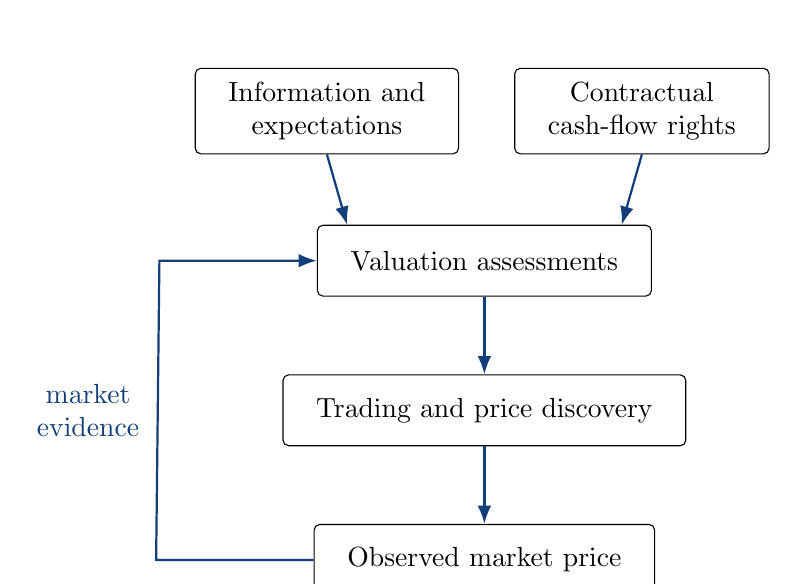
\begin{tikzpicture}[
  >=Latex,
  box/.style={
    draw,
    rounded corners=2pt,
    align=center,
    minimum height=0.9cm,
    inner xsep=12pt,
    inner ysep=5pt
  },
  flow/.style={
    -Latex,
    line width=0.8pt,
    FinanceBlue
  }
]

% Top nodes
\node[box] (info) at (-2.0,2.2)
{Information and\\expectations};

\node[box] (contract) at (2.0,2.2)
{Contractual\\cash-flow rights};

% Central sequence
\node[box] (valuation) at (0,0.3)
{Valuation assessments};

\node[box] (trading) at (0,-1.6)
{Trading and price discovery};

\node[box] (price) at (0,-3.5)
{Observed market price};

% Main flows: 90-degree turns
\coordinate (val-left) at
  ($(valuation.north west)!0.09!(valuation.north east)$);
\draw[flow]
  (info.south) -- (val-left);

\coordinate (val-right) at
  ($(valuation.north west)!0.91!(valuation.north east)$);

\draw[flow]
  (contract.south) -- (val-right);


% Vertical flows
\draw[flow]
  (valuation.south) -- (trading.north);

\draw[flow]
  (trading.south) -- (price.north);

% Feedback from observed market price to valuation
\draw[flow]
  (price.west)
  -- ++(-2.0,0)
  -- node[left, midway, align=center, xshift=-3pt]
     {market\\evidence}
     ($(valuation.west)+(-2.0,0)$)
  -- (valuation.west);

\end{tikzpicture}

\caption{Information, contractual rights, valuation, and market prices}
\label{fig:ch5-value-formation}

\end{figure}

Figure~\ref{fig:ch5-value-formation} summarizes these interactions. Information affects expectations about future cash flows and risk, while contracts define the cash-flow rights attached to each claim. These factors enter valuation, which in turn informs trading decisions. Trading and price discovery generate observed market prices, which provide market evidence for assessing and revising valuations.

Figure~\ref{fig:ch5-value-formation} summarizes these interactions. Information shapes expectations about future cash flows and risk, while contractual terms define the cash-flow rights attached to each claim. Valuation combines these inputs and informs trading decisions. Trading and price discovery produce market prices, which in turn provide evidence for assessing and revising valuations.

\begin{tcolorbox}[
  enhanced,
  breakable,
  colback=white,
  colframe=FinanceBlue,
  boxrule=0.7pt,
  sharp corners,
  borderline west={2.2pt}{0pt}{FinanceBlue},
  title={Financial Perspective: Valuation as a Conditional Statement},
  coltitle=white,
  colbacktitle=FinanceBlue,
  fonttitle=\bfseries,
  before skip=1.2em,
  after skip=1.2em
]

A valuation estimate is conditional on the contractual cash-flow rights, the information available, the timing assumptions, and the treatment of risk used in the analysis. Changes in these inputs may change the estimated value. A sound valuation states its assumptions explicitly and applies them consistently, allowing the result to be evaluated and revised as information changes.

\end{tcolorbox}

%========================================================
% Summary
%========================================================

\TailModule{summary}{Summary}

Financial valuation translates future cash flows into current value. The object being valued is a financial claim, so valuation begins by identifying the cash flows and contractual rights attached to that claim. Payment priority, collateral, conversion rights, and other contractual provisions can cause claims on the same underlying assets to have different values.

The timing of cash flows matters, as cash flows occurring at different dates must be converted to values at a common date. Risk also affects value: two claims with the same expected payoff can have different values when their payoffs are distributed differently across future states. Required returns provide one way to incorporate risk into valuation, while state-price valuation makes the dependence of value on future states explicit.

Discounted cash-flow valuation combines forecasts of claim-specific cash flows with appropriate discount rates. Its reliability depends on consistent treatment of cash flows and required returns, realistic forecasts, and economically plausible terminal assumptions. Relative valuation uses the observed prices of comparable assets, but valuation multiples reflect differences in growth, risk, profitability, payout, and other fundamentals. Contingent-claim valuation values state-contingent payoffs using state prices and no-arbitrage relationships.

Information, contracts, and valuation are closely connected. Information affects expectations about future cash flows and risk, while contracts define the rights attached to each claim. Trading and price discovery generate observable market prices, which provide evidence for evaluating and revising valuations. A valuation is conditional on the information, contractual rights, timing assumptions, and treatment of risk used in the analysis. Its reliability depends on internal consistency, economic plausibility, and its relationship to available market evidence.

%========================================================
% Key Terms
%========================================================

\TailModule{keyterms}{Key Terms}

Financial valuation; financial claim; cash-flow right; present value; discount factor; required return; risk-free rate; risk premium; expected cash flow; discounted cash-flow valuation; net present value; terminal value; growing perpetuity; sensitivity analysis; relative valuation; comparable firm; market multiple; price--earnings ratio; enterprise value; contingent claim; state-contingent payoff; state price; law of one price; no-arbitrage; price discovery; market price

%========================================================
% Financial AI Lab
%========================================================

\TailModule{aiprompt}{Financial AI Lab}

\textbf{Lab: Auditing an AI-Generated Valuation}

Choose a publicly traded company and ask an AI system to produce a simplified discounted cash-flow valuation using publicly available information. Require the AI to state the claim being valued, the forecast horizon, the cash-flow measure, the growth assumptions, the terminal-value method, and the discount rate.

Audit the valuation in five stages.

\begin{enumerate}

\item \textbf{Identify the claim.}
Determine whether the valuation refers to equity or to the entire enterprise, and whether the cash flows and discount rate are defined consistently with that claim.

\item \textbf{Verify the calculations.}
Reproduce the present-value calculations independently. Check units, cash-flow timing, compounding, and the treatment of terminal value.

\item \textbf{Evaluate the economic assumptions.}
Examine whether the cash-flow forecasts are economically plausible, whether long-run growth can reasonably persist, whether reinvestment is consistent with growth, and whether the discount rate is appropriate for the risk of the claim.

\item \textbf{Conduct sensitivity analysis.}
Identify two key assumptions to which the estimated value is particularly sensitive and report how changes in those assumptions affect the valuation.

\item \textbf{Compare the valuation with market evidence.}
Compare the result with the observed market price and one simple relative-valuation measure. Ensure that the quantities being compared refer to the same claim. Do not treat either the AI estimate or the market price as necessarily correct; explain the assumptions or market factors that may account for the difference.

\end{enumerate}

The final submission should identify at least one issue in the AI-generated valuation that is not apparent from the final valuation estimate alone. The issue may involve calculation, economic assumptions, internal consistency, or verification against market evidence.

%========================================================
% Applied Problems
%========================================================

\TailModule{appprobs}{Applied Problems}

\begin{enumerate}

\item \textbf{Timing and present value.}

A claim pays RMB~5,000 in three years. The relevant annual discount rate is 6 \%.

\begin{enumerate}

\item Calculate the present value of the claim.

\item Recalculate the present value if the payment occurs in six years instead.

\item Explain why postponing the payment reduces its present value when the discount rate is positive.

\end{enumerate}


\item \textbf{NPV and required return.}

A project requires an initial investment of RMB~12 million and is expected to produce cash flows of RMB~3 million, RMB~4 million, RMB~5 million, and RMB~4 million at the end of years 1 through 4.

\begin{enumerate}

\item Calculate the project's NPV at a required return of 7 \%.

\item Recalculate the NPV at a required return of 11 \%.

\item Explain why the project's value changes even though its expected cash flows remain unchanged.

\end{enumerate}


\item \textbf{Terminal-value sensitivity.}

A business is expected to generate cash flow of RMB 20 million in year 6, the first year after the explicit forecast period. From year 7 onward, cash flow is expected to grow at a constant annual rate \(g\) indefinitely. Assume that the year-6 cash flow remains unchanged across all scenarios.

\begin{enumerate}

\item Calculate the terminal value at the end of year 5 if $r=9\%$ and $g=3\%$.

\item Recalculate the terminal value if $g=4\%$, holding $r$ unchanged.

\item Recalculate the terminal value if $r=8\%$ and $g=3\%$.

\item Compare the results in parts (b) and (c). Explain why a one-percentage-point increase in $g$  and a one-percentage-point decrease in $r$ produce the same terminal value under the stated assumptions.

\end{enumerate}


\item \textbf{Relative valuation and consistency.}

Firm A has an enterprise value of RMB~8 billion and EBITDA of RMB~800 million. Firm B has EBITDA of RMB~500 million.

\begin{enumerate}

\item Calculate Firm A's EV/EBITDA multiple.

\item Apply this multiple to Firm B to estimate its implied enterprise value.

\item Suppose Firm B has RMB~1.2 billion of net debt. Calculate its implied equity value.

\item Explain why an enterprise-value multiple should not be applied directly to an earnings measure attributable only to equity holders.

\end{enumerate}


\item \textbf{State-price valuation.}

There are two equally likely future states. Claim A pays 140 in the strong state and 60 in the weak state. Claim B pays 80 in the strong state and 120 in the weak state.

\begin{enumerate}

\item Calculate the expected payoff of each claim.

\item Suppose the state prices are $q_S=0.38$ and $q_W=0.56$. Calculate the  values of each claim at date 0.

\item Compare the expected payoffs and the values of two claim at date 0.

\item Explain why equal expected payoffs need not imply equal values at date 0.

\end{enumerate}


\item \textbf{Contractual allocation of value.}

A firm will generate cash flow of either 150 or 70 next period, with each state equally likely. It has debt promising repayment of 100.

\begin{enumerate}

\item Calculate the payoffs to debt and equity in each state.

\item Verify that the debt and equity payoffs sum to the firm's total cash flow in each state.

\item Using state prices $q_H=0.40$ and $q_L=0.55$, calculate the current values of debt, equity, and the firm as a whole.

\item Verify that the values of debt and equity sum to the value of the firm.

\end{enumerate}

\end{enumerate}

%========================================================
% Further Reading
%========================================================

\TailModule{furtherread}{Further Reading}

\begin{itemize}

\item Fisher, Irving (1930), 
\emph{The Theory of Interest: As Determined by Impatience to Spend Income and Opportunity to Invest It}, 
Macmillan.

\item Williams, John Burr (1938), 
\emph{The Theory of Investment Value}, 
Harvard University Press.

\item Modigliani, Franco, and Merton H. Miller (1958), 
``The Cost of Capital, Corporation Finance and the Theory of Investment,'' 
\emph{The American Economic Review}, 48(3), 261--297.

\item Sharpe, William F. (1964), 
``Capital Asset Prices: A Theory of Market Equilibrium under Conditions of Risk,'' 
\emph{The Journal of Finance}, 19(3), 425--442.

\item Damodaran, Aswath (2012), 
\emph{Investment Valuation: Tools and Techniques for Determining the Value of Any Asset}, 
3rd ed., Wiley.

\end{itemize}

\ChapterTail{summary,keyterms,aiprompt,appprobs,furtherread}


\part{Financial Markets}
\chapter{Interest Rates and Capital Allocation}
\label{chap:Interest_Rates_and_Capital_Allocation}

\begin{openingcase}{Which Interest Rate Matters?}

A firm is considering a one-year investment that requires RMB~10 million today and is expected to generate RMB~10.6 million one year from now. At first glance, the decision appears simple: compare the project's 6\% expected return with ``the interest rate.''

But which interest rate?

A bank may quote one borrowing rate, while a government security of the same maturity offers another. Rates may also differ with maturity, inflation expectations, credit risk, and liquidity. There is therefore no single market interest rate that applies to every financial decision.

The firm's project may be attractive at one required return and unattractive at another. Understanding why market rates differ, and how those differences affect financing and investment decisions, is central to understanding how financial markets allocate capital.

\end{openingcase}

\begin{tcolorbox}[
  enhanced,
  colback=FinanceBlue!6,
  colframe=FinanceBlue,
  boxrule=0.6pt,
  sharp corners,
  left=8pt,
  right=8pt,
  top=7pt,
  bottom=7pt,
  before skip=1em,
  after skip=1.6em,
  title=\textbf{Core Questions},
  coltitle=white,
  colbacktitle=FinanceBlue,
  fonttitle=\bfseries,
  attach boxed title to top left={xshift=6pt,yshift=-2mm},
  boxed title style={
    boxrule=0pt,
    sharp corners,
    left=5pt,
    right=5pt,
    top=2pt,
    bottom=2pt
  }
]
\begin{enumerate}[
  leftmargin=*,
  label=\textcolor{FinanceBlue}{\textbf{\arabic*.}},
  itemsep=0.55em,
  topsep=0.2em
]

\item Why is an interest rate a price of intertemporal exchange rather than simply a borrowing cost?

\item Why do interest rates differ across maturities, borrowers, and financial instruments?

\item How do interest rates influence saving, borrowing, investment, and the allocation of capital?

\end{enumerate}
\end{tcolorbox}

\section{Interest Rates as the Price of Intertemporal Exchange}

An interest rate is the price at which purchasing power today is exchanged for purchasing power in the future. It determines the return associated with postponing the use of funds and the cost of obtaining funds before future income becomes available.

\subsection{Intertemporal Choice and the Opportunity Cost of Funds}

For a one-period investment, one unit of purchasing power today grows to \(1+r\) next period. Equivalently, the present value of one unit received next period is

\[
PV_0=\frac{1}{1+r}.
\]

This relationship expresses the same intertemporal price in terms of both future returns and present values.

Saving, borrowing, and investment decisions involve comparing alternative uses or sources of funds. A saver considers the return available from postponing consumption, a borrower evaluates the cost of alternative financing arrangements, and an investor compares a project's expected return with that of other feasible investments. The relevant opportunity cost is determined by the best available alternative, with risk, maturity, and liquidity taken into account.

Suppose an investor can earn 4\% on a one-year security with risk comparable to that of a proposed project. If the project is expected to return only 3\%, the alternative security offers the higher return for comparable risk and maturity.

This opportunity-cost principle connects market interest rates directly to capital allocation. Let a project require investment $I_0$ today and generate a certain payoff $CF_1$ one period later. If the opportunity cost of funds is $r$, the project creates value when

\begin{equation*}
\frac{CF_1}{1+r}>I_0.
\label{eq:ch6-one-period-investment-condition}
\end{equation*}

Equivalently,

\begin{equation*}
\frac{CF_1-I_0}{I_0}>r.
\label{eq:ch6-return-hurdle-simple}
\end{equation*}

The relevant opportunity cost is the return on a comparable alternative with similar risk and maturity. Differences in risk or maturity therefore imply different required returns.

In actual markets, borrowing and lending rates may differ, and borrowers may face different credit spreads. These differences affect the opportunity costs faced by market participants.

\begin{example}{Opportunity Cost and a One-Year Investment}{opportunity-cost-one-year-investment}

Suppose a firm can invest RMB~10 million in a one-year project that will produce a certain RMB~10.5 million. The project return is 5\%.

If the relevant opportunity cost is 3\%, the present value of the payoff is

$$
PV=\frac{10.5}{1.03}=10.19
$$
million RMB, giving the project a positive NPV. If the opportunity cost rises to 6\%,

$$
PV=\frac{10.5}{1.06}=9.91
$$
million RMB, and the project has a negative NPV.

The cash flow is unchanged; the higher opportunity cost changes the investment decision.

\end{example}



\subsection{Interest Rate Quotations, Compounding, and Effective Rates}

Interest rates describe the exchange of purchasing power across time, but the amount accumulated over a given horizon depends on how interest is calculated. Financial-market quotations specify the period to which a rate applies and the associated compounding convention.

Let $r$ denote the interest rate per period. If $P_0$ is invested for one period, its future value is

\begin{equation}
P_1=P_0(1+r).
\label{eq:ch6-one-period-growth}
\end{equation}

If the investment extends over $T$ periods and interest is compounded once per period,

\begin{equation}
P_T=P_0(1+r)^T.
\label{eq:ch6-compound-growth}
\end{equation}

Under compound interest, interest earned in each period is added to principal and earns interest in subsequent periods. By contrast, under simple interest, interest is calculated only on the initial principal:

\begin{equation}
P_T=P_0(1+rT).
\label{eq:ch6-simple-interest}
\end{equation}

For positive interest rates, the difference between simple and compound interest increases with the investment horizon. For example, RMB~100 invested for three years at 5\%grows to

$$
100(1+0.05\times 3)=115
$$
under simple interest and to

$$
100(1.05)^3=115.76
$$
under annual compounding. The compounding convention therefore affects the effective return represented by a quoted rate.

\paragraph{Nominal annual rates and compounding frequency.}

Many market interest rates are quoted on an annual basis even when interest is compounded more frequently. Let $j$ denote a nominal annual rate compounded $m$ times per year. The periodic rate is

\begin{equation}
r=\frac{j}{m}.
\end{equation}

The corresponding effective annual rate, denoted $EAR$, is

\begin{equation}
EAR=
\left(1+\frac{j}{m}\right)^m-1.
\label{eq:ch6-ear}
\end{equation}

The effective annual rate measures the one-year return implied by the nominal rate and its compounding frequency. For a given nominal annual rate, more frequent compounding produces a higher effective annual rate, as shown in Table~\ref{tab:ch6-compounding-frequency}.

\begin{table}[H]
\centering
\caption{A 6\%nominal annual rate under different compounding frequencies}
\label{tab:ch6-compounding-frequency}

\begin{tabular}{@{}l c c@{}}
\toprule
\textbf{Compounding} & \textbf{Periods per year} & \textbf{Effective annual rate} \\
\midrule
Annual & 1 & 6.000\% \\
Semiannual & 2 & 6.090\% \\
Quarterly & 4 & 6.136\% \\
Monthly & 12 & 6.168\% \\
\bottomrule
\end{tabular}
\end{table}

The effective annual rate provides a common basis for comparing rates quoted with different compounding frequencies.
\paragraph{Continuous compounding.}

As the compounding frequency increases, discrete compounding approaches continuous compounding. Let $r_c$ denote the continuously compounded annual rate. Over $T$ years,

\begin{equation}
P_T=P_0 e^{r_c T}.
\label{eq:ch6-continuous-compounding}
\end{equation}

The continuously compounded rate and the effective annual rate are related by

\begin{equation}
EAR=e^{r_c}-1,
\label{eq:ch6-continuous-to-ear}
\end{equation}
or equivalently,

\begin{equation}
r_c=\ln(1+EAR).
\label{eq:ch6-ear-to-continuous}
\end{equation}

Continuous compounding is particularly convenient for comparing rates across horizons and is widely used in financial modeling.

\paragraph{Rates over fractions of a year.}

Interest rates may also need to be expressed over horizons shorter than one year. If $EAR$ is the effective annual rate, the compound rate over a fraction $\tau$ of a year is

\begin{equation}
r_{\tau}=(1+EAR)^{\tau}-1.
\label{eq:ch6-fractional-period-rate}
\end{equation}

This conversion assumes compound interest over the fractional period. In practice, some markets use different quotation and day-count conventions, particularly for money-market instruments.

\begin{tcolorbox}[
enhanced,
breakable,
colback=white,
colframe=FinanceBlue,
boxrule=0.7pt,
sharp corners,
borderline west={2.2pt}{0pt}{FinanceBlue},
title=\textbf{Financial Perspective: Compare Like with Like},
coltitle=white,
colbacktitle=FinanceBlue,
fonttitle=\bfseries,
before skip=1.2em,
after skip=1.2em
]

Interest rates should be placed on a common basis before they are compared. Differences in time horizon, compounding frequency, day-count convention, or nominal versus effective quotation can produce different effective returns from the same stated percentage rate.

\end{tcolorbox}


\subsection{Nominal and Real Interest Rates}

A nominal interest rate measures the return on funds in monetary terms, whereas a real interest rate measures the return in terms of purchasing power. The distinction arises when the price level changes: part of the nominal return may reflect higher prices rather than an increase in the quantity of goods and services that the future amount can purchase.

Suppose one unit of currency grows to $1+i$ over one year, where $i$ is the nominal interest rate. If the price level rises by rate $\pi$ over the same period, the purchasing power of the future amount relative to today's price level grows by

\begin{equation}
1+r
=
\frac{1+i}{1+\pi},
\label{eq:ch6-fisher-exact}
\end{equation}
where $r$ is the realized real interest rate.

Rearranging this relation gives the exact Fisher equation:

\begin{equation}
i=r+\pi+r\pi.
\label{eq:ch6-fisher-expanded}
\end{equation}

For moderate values of $r$ and $\pi$, the cross-product term $r\pi$ is small relative to the linear terms, yielding the approximation

\begin{equation}
i\approx r+\pi.
\label{eq:ch6-fisher-approx}
\end{equation}

For decisions made before inflation is known, expected rather than realized inflation is relevant. If $\pi^e$ denotes expected inflation and $r^e$ the expected real interest rate, the approximate Fisher relation is

\begin{equation}
i\approx r^e+\pi^e.
\label{eq:ch6-fisher-expected}
\end{equation}

The difference between expected and realized inflation affects the realized real return on a fixed nominal claim relative to its expected real return. Suppose a lender makes a one-year fixed-rate loan at a nominal interest rate of 6\%, when inflation is expected to be 2\%. The expected real return is approximately 4\%. If realized inflation is instead 5\%, the realized real return falls to about 1\%.

Unexpected inflation therefore redistributes purchasing power between borrowers and lenders under fixed nominal contracts. Higher-than-expected inflation reduces the lender's realized real return and benefits the borrower relative to the original terms; lower-than-expected inflation has the opposite effect.

Nominal and real interest rates serve different analytical purposes. Financial contracts are commonly stated in nominal terms: borrowers make nominal payments, bonds promise nominal coupons, and policy rates are quoted in nominal terms. Real interest rates, by contrast, measure returns and financing costs in terms of purchasing power. They are particularly useful when saving, investment, and capital-allocation decisions are evaluated in real terms. The relation between nominal rates and expected inflation links nominal financial contracts to their real economic implications.

\section{Determinants of Interest Rates}

Interest rates are market prices influenced by several interacting forces. These include the supply and demand for funds, inflation expectations, monetary and liquidity conditions, and differences in risk and maturity. Their relative importance varies across markets, instruments, and maturities.

\subsection{Saving, Investment, and the Demand for Funds}

A simple starting point treats the interest rate as the price that balances the supply of funds with the demand for funds. Savers make funds available by postponing current expenditure, while borrowers seek funds to finance investment and other expenditures.

Let the supply of funds be

\begin{equation}
S=S(r),
\qquad
S'(r)>0,
\label{eq:ch6-saving-supply}
\end{equation}
and the demand for funds be

\begin{equation}
D=D(r),
\qquad
D'(r)<0.
\label{eq:ch6-investment-demand}
\end{equation}

The equilibrium rate $r^{*}$ satisfies

\begin{equation}
S(r^{*})=D(r^{*}).
\label{eq:ch6-funds-equilibrium}
\end{equation}

The upward-sloping supply curve reflects the tendency for a higher interest rate to make postponing current expenditure more attractive. The downward-sloping demand curve reflects the tendency for a higher interest rate to reduce the number of investment opportunities whose expected returns exceed the cost of funds.


\begin{figure}[H]
\centering
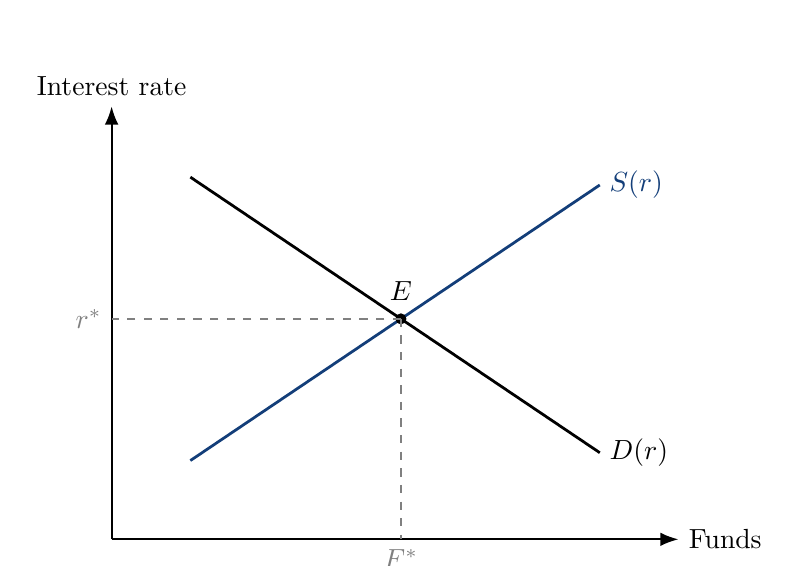
\begin{tikzpicture}[
  >=Latex,
  axis/.style={-Latex, line width=0.8pt},
  curve/.style={line width=1.0pt},
  guide/.style={dashed, gray, line width=0.6pt}
]

\draw[axis] (0,0) -- (7.2,0) node[right] {Funds};
\draw[axis] (0,0) -- (0,5.5) node[above] {Interest rate};

\draw[curve, FinanceBlue] (1.0,1.0) -- (6.2,4.5);
\draw[curve] (1.0,4.6) -- (6.2,1.1);

\node[FinanceBlue, right] at (6.2,4.5) {$S(r)$};
\node[right] at (6.2,1.1) {$D(r)$};

\coordinate (E) at (3.674,2.80);
\fill (E) circle (2pt);
\node[above, yshift=3pt] at (E) {$E$};

\draw[guide] (E) -- (0,2.80) node[left] {$r^{*}$};
\draw[guide] (E) -- (3.674,0) node[below] {$F^{*}$};

\end{tikzpicture}
\caption{A stylized market for funds}
\label{fig:ch6-funds-market}
\end{figure}

The model provides a simple framework for comparative statics. An increase in expected productivity or other profitable investment opportunities shifts the demand curve for funds to the right. Other things equal, both the equilibrium interest rate and the quantity of funds increase. Greater willingness to save at each interest rate shifts the supply curve for funds to the right, lowering the equilibrium interest rate and increasing the equilibrium quantity of funds.

These results describe comparative statics within a stylized model rather than a complete theory of market interest rates. In actual financial systems, financing conditions also reflect monetary policy, bank balance sheets, capital flows, and institutional constraints. The supply of funds should not be interpreted as a fixed stock of prior saving available for lending. The framework provides a simple model of how shifts in the supply of and demand for funds affect interest rates and the volume of financing.


\subsection{Inflation Expectations and Monetary Conditions}

Expected inflation affects nominal interest rates by changing the nominal return required to preserve purchasing power. For a given expected real rate, higher expected inflation is associated with a higher nominal interest rate, as indicated by the Fisher relation.

The response need not be one-for-one. Expected real rates may also change, risk premia may move, and monetary policy may respond to inflation expectations. The Fisher relation identifies one component of nominal interest rates rather than providing a complete explanation of observed rate movements.

Monetary conditions are particularly important for short-term nominal rates. Central banks typically influence short-term market rates through policy rates and the conditions under which reserves and short-term funding are supplied. Changes in the policy stance can also affect longer-term rates through expectations of future short rates, inflation, economic activity, and risk premia.

A lower policy rate may reduce short-term funding costs. If the lower stance is expected to persist, longer-maturity yields may also fall. If inflation expectations rise, however, long-term nominal yields may fall less or even increase. Wider risk or liquidity premia can likewise raise borrowing costs for some private borrowers even when the policy rate declines.

\subsection{Risk Structure and Interest-Rate Spreads}

Interest-rate differences across otherwise comparable instruments of the same maturity form the risk structure of interest rates. Credit risk and market liquidity are major determinants of these differences, while contractual, tax, and institutional factors can also affect required returns.

\paragraph{Credit risk.}

Credit risk arises from the possibility that promised payments will not be made in full or on time. Greater expected credit losses or greater uncertainty about repayment generally raise the return required by investors. In debt markets, the difference in rates relative to a comparable low-risk benchmark is commonly referred to as a credit spread.

\begin{example}{Credit Risk and the Required Return} {credit-risk-required-return}

Suppose a one-year low-risk government security offers a return of 3\%, while a one-year corporate debt instrument with otherwise comparable characteristics requires a return of 5.5\%. The difference is

\[
5.5\%-3.0\%=2.5\%
\]
and represents the corporate instrument's credit spread relative to the benchmark.

The higher required return reflects the possibility that the promised corporate payments may not be made in full or on time. The spread need not equal expected credit loss, since investors may also require compensation for uncertainty about repayment.

\end{example}

Risk compensation depends not only on expected loss but also on the states in which losses occur. Two one-year instruments can have the same expected payoff yet differ in the states in which losses are concentrated. An instrument that delivers lower payoffs mainly during recessions provides less protection when investors' income and the value of their other assets are also likely to be low. It may therefore require greater compensation than an instrument whose lower payoffs occur mainly in strong economic conditions.

Other risks can affect required returns insofar as they alter expected cash flows, repayment risk, or investors' exposure to adverse states.


\begin{table}[htbp]
\centering
\caption{Factors Affecting Required Returns on Comparable Instruments}
\label{tab:ch6-rate-differences}

\begin{tabularx}{\textwidth}{@{}p{3.2cm}Y Y@{}}
\toprule
\textbf{Factor} &
\textbf{Economic reason} &
\textbf{Effect on required return} \\
\midrule

Credit risk &
Promised payments may be delayed, reduced, or not made in full &
Expected credit losses and compensation for bearing default risk can raise the required return \\

Exposure to adverse states &
Payoffs may be low when investors' income and the value of their other assets are also weak &
Such exposure provides less protection in adverse conditions and can increase required compensation \\

Market liquidity &
The instrument may be costly to sell quickly without a substantial price concession &
Lower liquidity can raise the required return \\

Contractual features &
Embedded options and other provisions alter the timing and distribution of future cash flows &
The effect on required return depends on how these features affect payoffs and risk for each party \\

Tax and institutional treatment &
Tax rules, collateral eligibility, and regulatory constraints can affect the net benefits of holding an instrument &
Differences in after-tax returns and institutional benefits can lead to different required returns \\

\bottomrule
\end{tabularx}
\end{table}

\paragraph{Market liquidity.}

Market liquidity affects the ease with which an instrument can be sold without a substantial price concession. Investors generally value greater liquidity, while less liquid instruments may require higher returns than otherwise comparable instruments.

Liquidity can deteriorate during periods of financial stress. Dealers may reduce inventories, funding conditions may tighten, and buyers may demand larger price concessions. Deteriorating liquidity can widen interest-rate spreads even when expected credit losses change little.

\paragraph{Benchmark rates and spreads.}

Market interest rates are often compared with a benchmark rate, which serves as a reference for instruments of similar maturity. The difference between an instrument's rate and the benchmark is its spread. For instrument $i$ with maturity $T$,

\begin{equation}
r_{i,T}=r_{b,T}+s_{i,T},
\label{eq:ch6-benchmark-spread}
\end{equation}
where $r_{b,T}$ is the benchmark rate for maturity $T$ and $s_{i,T}$ is the spread of instrument $i$ over that benchmark. Changes in the instrument's rate can then be written as

\begin{equation}
\Delta r_{i,T}=\Delta r_{b,T}+\Delta s_{i,T}.
\label{eq:ch6-benchmark-spread-change}
\end{equation}

If rates on many instruments of the same maturity move together, changes in the benchmark rate may explain much of the movement. Monetary conditions and inflation expectations can contribute to such common changes. When the benchmark rate changes little but rates on particular instruments rise, wider spreads may reflect greater credit risk, lower market liquidity, or other instrument-specific factors.

Observed spreads do not reveal a single underlying cause. Credit conditions, market liquidity, contractual features, tax treatment, regulation, and investor demand may all affect the spread over a benchmark rate.

Figure~\ref{fig:ch6-china-10y-yields} illustrates these
patterns using ten-year yields from China's bond market.
Since all series have the same maturity, common movements
may reflect changes in market-wide conditions, while
differences in yield levels may reflect credit risk,
liquidity, and other instrument-specific characteristics.

\begin{figure}[H]
\centering

\includegraphics[width=0.9\textwidth]{ChinaBond_10Y_Yields_2016_2026.pdf}

\caption{Ten-year ChinaBond yields across selected bond categories, 2016--2026}
\label{fig:ch6-china-10y-yields}

\vspace{0.15em}

\begin{minipage}{0.9\textwidth}
\footnotesize
\noindent\textit{Source: China Central Depository \& Clearing Co., Ltd. (ChinaBond).}
\end{minipage}

\end{figure}

Comparisons across different maturities introduce another
dimension of interest-rate differences, giving rise to
the term structure of interest rates.

\section{The Term Structure of Interest Rates}

The term structure of interest rates describes the relationship between interest rates and maturity for otherwise comparable instruments. Its graphical representation is a yield curve.

\subsection{Spot Rates, Forward Rates, and Yield Curves}

A spot rate is the annualized interest rate applicable today
to a zero-coupon claim that makes a single payment at a
specified future date. A forward rate is the rate implied
today for borrowing or lending over a future interval.

Let $s_t$ denote the annualized $t$-period spot rate for
a default-free zero-coupon claim. Under annual compounding,
the present value of one unit paid at date $t$ is

\begin{equation}
P(0,t)=\frac{1}{(1+s_t)^t}.
\label{eq:ch6-spot-discount-factor}
\end{equation}

For example, suppose the one-year spot rate is 3\% and
the two-year spot rate is 4\%. The corresponding discount
factors are

\[
P(0,1)=\frac{1}{1.03},
\qquad
P(0,2)=\frac{1}{(1.04)^2}.
\]

To derive the one-year forward rate beginning one year
from today, let $f_{1,2}$ denote this rate. Under
no-arbitrage, investing for two years at the two-year
spot rate must generate the same terminal value as
investing for one year at the one-year spot rate and
then reinvesting at the forward rate. Thus,

\begin{equation}
(1+s_2)^2
=
(1+s_1)(1+f_{1,2}),
\label{eq:ch6-forward-from-spot}
\end{equation}
where $s_1$ and $s_2$ are the one-year and two-year
spot rates. Hence,

\begin{equation}
f_{1,2}
=
\frac{(1+s_2)^2}{1+s_1}-1.
\label{eq:ch6-forward-rate}
\end{equation}

Using the rates in the example, the implied forward
rate is approximately 5.01\%. The forward rate is not the arithmetic difference between
spot rates.

More generally, let $s_m$ and $s_n$ denote the
$m$-year and $n$-year spot rates, and let $f_{m,n}$
denote the annualized forward rate from year $m$
to year $n$, where $n>m$. Under annual compounding,

\begin{equation}
f_{m,n}
=
\left[
\frac{(1+s_n)^n}{(1+s_m)^m}
\right]^{\frac{1}{n-m}}
-1.
\label{eq:ch6-general-forward-rate}
\end{equation}

Plotting zero-coupon spot rates against their maturities
produces a spot-rate curve, which is a yield curve
constructed from zero-coupon rates. In broader market
usage, a yield curve plots yields on comparable debt
securities against maturity. Yields to maturity on
coupon-bearing bonds need not equal spot rates.


\begin{example}{Constructing a Spot-Rate Curve}
{spot-rate-curve}

Suppose the annual spot rates for maturities of one, two, three, five, and ten years are:

\begin{center}
\begin{tabular}{lccccc}
\toprule
\textbf{Maturity (years)} & 1 & 2 & 3 & 5 & 10 \\
\midrule
\textbf{Spot rate (\%)} & 3.00 & 4.00 & 4.40 & 4.70 & 4.90 \\
\bottomrule
\end{tabular}
\end{center}

Plotting these rates against maturity gives the spot-rate curve shown below.

\begin{center}
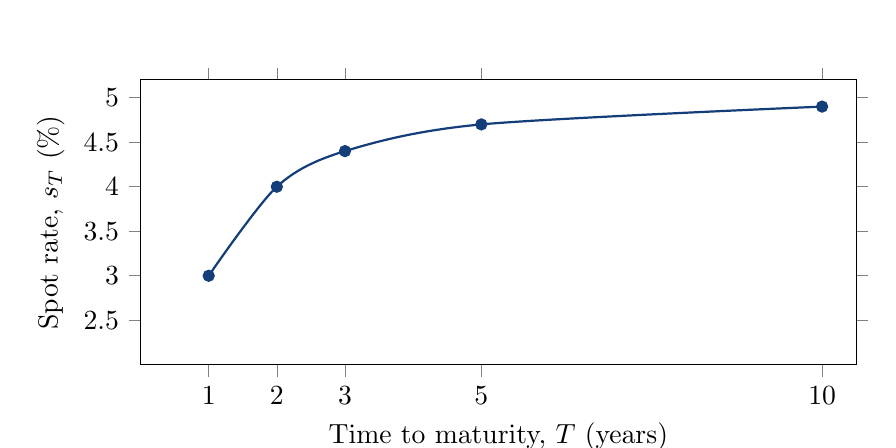
\begin{tikzpicture}

\begin{axis}[
    width=0.88\linewidth,
    height=5.2cm,
    xmin=0,
    xmax=10.5,
    ymin=2.0,
    ymax=5.2,
    xtick={1,2,3,5,10},
    ytick={2.5,3.0,3.5,4.0,4.5,5.0},
    xlabel={Time to maturity, $T$ (years)},
    ylabel={Spot rate, $s_T$ (\%)},
    axis lines=box,
    tick align=outside,
    enlargelimits=false,
    grid=none,
]

\addplot[
    FinanceBlue,
    thick,
    smooth,
    mark=*,
    mark size=1.8pt
]
coordinates {
    (1,3.00)
    (2,4.00)
    (3,4.40)
    (5,4.70)
    (10,4.90)
};

\end{axis}

\end{tikzpicture}
\end{center}
\end{example}



\begin{figure}[H]
\centering

\includegraphics[width=1.0\textwidth]{China_Government_Yield_Curves_Typical.pdf}

\caption{Selected Chinese government bond yield curves}
\label{fig:ch6-china-gov-yield-curves}

\vspace{0.15em}
\begin{minipage}{1.0\textwidth}
\footnotesize
\noindent\textit{Source: China Central Depository \& Clearing Co., Ltd. (ChinaBond); authors' calculations.}
\end{minipage}

\end{figure}

Spot-rate curves may be upward sloping, approximately flat, inverted, or more complex. Market yield curves exhibit similar configurations. Figure~\ref{fig:ch6-china-gov-yield-curves} shows selected examples from China's government bond market.

Traditional theories of the term structure explain these configurations through expectations about future short-term rates, market segmentation across maturities, and investors' preferred maturity habitats. Modern term-structure analysis commonly decomposes longer-term rates into an expected path of short-term rates and a time-varying term premium. 

\subsection{The Expectations Hypothesis}
The pure expectations hypothesis holds that bonds of different maturities are perfect substitutes in investors' portfolios. Investors base their maturity choices on expected returns and do not require an additional term premium for holding longer-term bonds. 

Consider a two-year horizon and one unit of funds invested today. An investor can follow either of two strategies. The first is to invest for two years at the current two-year spot rate $s_2$. The second is to invest for one year at the current one-year spot rate $s_1$ and then reinvest for the second year at the one-year short rate prevailing at that time. Let $\widetilde{r}_{1,2}$ denote the one-year short rate that will prevail between years 1 and 2. At time 0, this rate is not yet known, and its current expectation is $\mathrm{E}_0[\widetilde{r}_{1,2}]$.

\begin{figure}[H]
\centering

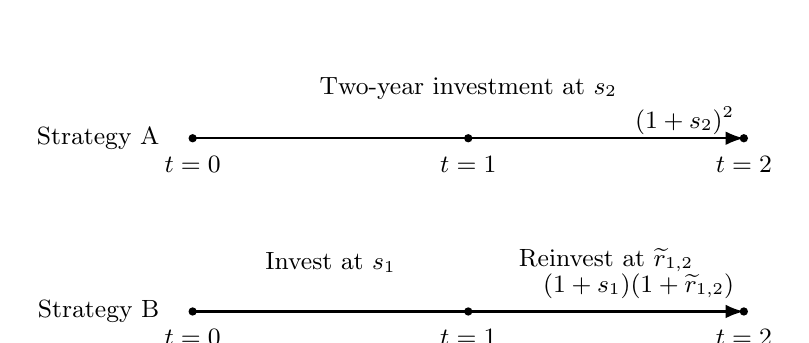
\begin{tikzpicture}[
    >=Latex,
    timeline/.style={line width=0.8pt},
    lab/.style={font=\small}
]

% Strategy A
\node[lab, anchor=east] at (-0.3,2.2) {Strategy A};

\draw[timeline,->] (0,2.2) -- (7,2.2);

\foreach \x/\t in {0/0,3.5/1,7/2} {
    \fill (\x,2.2) circle (1.5pt);
    \node[lab, below=3pt] at (\x,2.2) {$t=\t$};
}

\node[lab, above=5pt] at (3.5,2.4)
    {Two-year investment at $s_2$};

\node[lab, above=5pt, anchor=east] at (7,2.25)
    {$(1+s_2)^2$};


% Strategy B
\node[lab, anchor=east] at (-0.3,-0.0) {Strategy B};

\draw[timeline,->] (0,-0.0) -- (7,-0.0);

\foreach \x/\t in {0/0,3.5/1,7/2} {
    \fill (\x,-0.0) circle (1.5pt);
    \node[lab, below=3pt] at (\x,-0.0) {$t=\t$};
}

\node[lab, above=5pt] at (1.75,0.2)
    {Invest at $s_1$};

\node[lab, above=5pt] at (5.25,0.2)
    {Reinvest at $\widetilde{r}_{1,2}$};

\node[lab, above=5pt, anchor=east] at (7,0.15)
    {$(1+s_1)(1+\widetilde{r}_{1,2})$};

\end{tikzpicture}

\caption{Two investment strategies over a two-year horizon}
\label{fig:ch6-expectations-strategies}
\end{figure}

Figure~\ref{fig:ch6-expectations-strategies} compares the two strategies over the two-year horizon. They produce $(1+s_2)^2$ and $(1+s_1)(1+\widetilde{r}_{1,2})$, respectively. Under the pure expectations hypothesis, bonds of different maturities are perfect substitutes.
Investors are therefore indifferent between the two
strategies, which must offer equal expected returns
over the same investment horizon:

\begin{equation}
(1+s_2)^2=(1+s_1)
\left(1+\mathrm{E}_0[\widetilde{r}_{1,2}]\right).
\label{eq:ch6-expectations-gross}
\end{equation}

Expanding Equation~(\ref{eq:ch6-expectations-gross}) yields

\[
1+2s_2+s_2^2
=
1+s_1+\mathrm{E}_0[\widetilde{r}_{1,2}]
+s_1\mathrm{E}_0[\widetilde{r}_{1,2}].
\]

When interest rates are moderate, the second-order terms are small. Ignoring these terms gives

\begin{equation}
s_2
\approx
\frac{s_1+\mathrm{E}_0[\widetilde{r}_{1,2}]}{2}.
\label{eq:ch6-expectations-two-year}
\end{equation}

The two-year spot rate is approximately the average of the current one-year spot rate and the expected one-year short rate between years 1 and 2.

The hypothesis also gives an interpretation to the forward rate. Combining Equation~(\ref{eq:ch6-expectations-gross}) with the forward-rate relation derived earlier gives

\begin{equation}
f_{1,2}
=
\mathrm{E}_0[\widetilde{r}_{1,2}].
\label{eq:ch6-forward-expectation}
\end{equation}

Under the expectations hypothesis, the forward rate equals the expected future short-term rate.

The same reasoning extends to longer maturities. The $n$-year spot rate is linked to the sequence of one-year forward rates by

\begin{equation}
(1+s_n)^n
=
(1+s_1)
\prod_{j=1}^{n-1}
(1+f_{j,j+1}).
\label{eq:ch6-spot-forward-general}
\end{equation}

Using
\[
f_{j,j+1}
=
\mathrm{E}_0[\widetilde{r}_{j,j+1}],
\]
the relation becomes

\begin{equation}
(1+s_n)^n
=
(1+s_1)
\prod_{j=1}^{n-1}
\left(1+\mathrm{E}_0[r_{j,j+1}]\right).
\label{eq:ch6-expectations-general-gross}
\end{equation}

For moderate interest rates, a first-order approximation gives

\begin{equation}
s_n
\approx
\frac{1}{n}
\left[
s_1
+
\sum_{j=1}^{n-1}
\mathrm{E}_0[r_{j,j+1}]
\right].
\label{eq:ch6-expectations-general}
\end{equation}

\begin{example}{Interpreting the Term Structure under the Expectations Hypothesis} {expectations-term-structure}

Suppose the current one-year spot rate is 3\%, and the expected one-year short rates for years 2 through 5 are 3.5, 4.0, 4.5, and 5.0\%. Under the expectations hypothesis,

\[
s_5
\approx
\frac{
3.0\%+3.5\%+4.0\%+4.5\%+5.0\%
}{5}
=
4.0\%.
\]

Under the expectations hypothesis, the five-year spot rate \(s_5\approx4.0\%\) exceeds the current one-year spot rate \(s_1=3.0\%\), reflecting expected future short-term rates that are, on average, higher than the current short-term rate.

\end{example}

Expectations alone do not determine the term structure when securities of different maturities are imperfect substitutes and supply and demand conditions differ across maturity segments.

\subsection{Market Segmentation and Preferred Habitat}

Investor demand may be concentrated in particular maturity ranges. Money-market funds and firms managing short-term liquidity needs tend to hold short-maturity instruments, while pension funds and life insurers often have long-dated liabilities that support demand for longer-maturity assets.

The market-segmentation theory treats securities of different maturities as imperfect substitutes. Supply and demand within each maturity segment can affect the corresponding interest rate. An increase in demand for long-term bonds, with supply unchanged, raises their prices and lowers their yields. Consequently, long-term rates may decline relative to short-term rates even when expectations of future short-term rates remain unchanged.

The preferred-habitat theory recognizes imperfect substitution across maturities. Investors may prefer particular maturity ranges but are willing to hold securities outside those ranges when expected compensation is sufficient. Maturity preferences can influence rates without implying complete segmentation of maturity markets.

The key distinction is the degree of substitution across maturities: market segmentation assumes very limited substitution, whereas preferred habitat allows investors to shift across maturities when compensation is sufficient.

Supply conditions can also vary across maturities. Changes in the maturity composition of government bond issuance, for example, alter the relative supply of short- and long-maturity securities and can influence their relative interest rates.

\subsection{Term Premia}

Modern term-structure analysis allows longer-term rates to differ from the expected path of future short-term rates through a time-varying term premium. Accordingly, forward rates need not equal expected future short-term rates.

Longer-maturity fixed-income securities are generally more sensitive to changes in market interest rates than otherwise similar shorter-maturity securities. When market rates rise, the present value of more distant fixed cash flows falls more sharply. This greater price sensitivity increases investors' exposure to interest-rate risk and is an important source of term premia.

Allowing for a term premium, the $n$-period spot rate can be represented approximately as

\begin{equation}
s_n
\approx
\frac{1}{n}
\left[
s_1
+
\sum_{j=1}^{n-1}
\mathrm{E}_0[r_{j,j+1}]
\right]
+
TP_n,
\label{eq:ch6-term-premium-decomposition}
\end{equation}
where $TP_n$ is the term premium, the component of the longer-term rate not accounted for by the expected path of short-term rates.

The sign and magnitude of the term premium can vary. A positive term premium indicates that investors require additional expected return for holding longer-maturity securities rather than repeatedly investing in shorter-maturity securities. The term premium can be lower when longer-maturity securities provide diversification or hedging benefits, and in some circumstances it can become negative.

An upward-sloping term structure can reflect expectations of higher future short-term rates, a positive term premium, or both. The slope alone does not reveal their relative contributions.

\begin{example}
{Decomposing the Same Long-Term Rate}
{term-premium-sources}

Example~\ref{ex:expectations-term-structure} showed that a five-year spot rate of $s_5\approx4.0\%$ can be consistent with a current one-year spot rate of $s_1=3.0\%$ and expected one-year short rates of $3.5\%$, $4.0\%$, $4.5\%$, and $5.0\%$ over years 2 through 5. Under the expectations hypothesis, this configuration implies $TP_5\approx0$.

Now retain $s_1=3.0\%$ and $s_5=4.0\%$, but suppose the expected one-year short rates for years 2 through 5 are all $3.0\%$. The expected path of short-term rates then averages 3.0 \%. Equation~(\ref{eq:ch6-term-premium-decomposition}) implies

\[
TP_5
\approx
4.0\%-3.0\%
=
1.0\%.
\]

The same five-year spot rate now reflects a positive term premium rather than expectations of higher future short-term rates.

\end{example}

Movements in long-term rates can reflect changes in either expected future short-term rates or the term premium. A rise driven by higher expected future short-term rates has a different economic interpretation from one driven primarily by a higher term premium. A higher term premium indicates that investors require greater compensation, over and above expected future short-term rates, for holding longer-maturity securities and bearing the associated interest-rate risk.

\begin{tcolorbox}[
  enhanced,
  breakable,
  colback=white,
  colframe=FinanceBlue,
  boxrule=0.7pt,
  sharp corners,
  borderline west={2.2pt}{0pt}{FinanceBlue},
  title=\textbf{Finance Perspective: Interpreting the Yield Curve},
  coltitle=white,
  colbacktitle=FinanceBlue,
  fonttitle=\bfseries,
  before skip=1.2em,
  after skip=1.2em
]


The slope of the yield curve should not be interpreted as a direct forecast of future short-term interest rates. Long-term rates can also reflect time-varying term premia and supply and demand conditions across maturities. The same observed yield curve can be consistent with different combinations of expectations, term premia, and maturity-specific supply and demand.
\end{tcolorbox}

\section{Capital Allocation and Investment Decisions}

Interest rates affect saving, borrowing, and investment decisions by changing the opportunity cost of funds. They affect how capital is allocated across alternative investments. Through these decisions, interest rates link financial-market prices to the allocation of real resources.

\subsection{Interest Rates and Saving, Borrowing, and Investment}

A change in interest rates alters the relative price of current and future consumption. For savers, a higher interest rate increases the future consumption supported by a given amount of current saving. This substitution effect tends to encourage saving. The overall response also depends on income and wealth effects. A net saver may increase current consumption as higher interest income raises lifetime resources, while a net borrower experiences the opposite effect. Aggregate saving need not respond uniformly to changes in interest rates.

Borrowing responds more directly to the cost of finance. A higher borrowing rate raises the future repayment required for a given amount borrowed and tends to reduce credit demand. This response may be amplified when higher rates interact with adverse selection, collateral constraints, or lender balance-sheet conditions, reducing both credit demand and credit availability.

Investment responds to changes in the opportunity cost of funds. An increase in market interest rates raises the returns available on alternative financial claims and, other things equal, increases the required return on investment. Investment opportunities with relatively low prospective returns become less likely to receive financing, while those offering returns sufficient to compensate for their risk remain more attractive.

At the aggregate level, changes in required returns affect both aggregate investment and the allocation of capital. A common change in market interest rates need not affect all investment opportunities equally, since projects differ in their expected returns and risks, while borrowers face different financing conditions. Interest-rate changes can therefore influence not only the overall level of investment but also the distribution of capital across investment uses.

\begin{figure}[H]
\centering
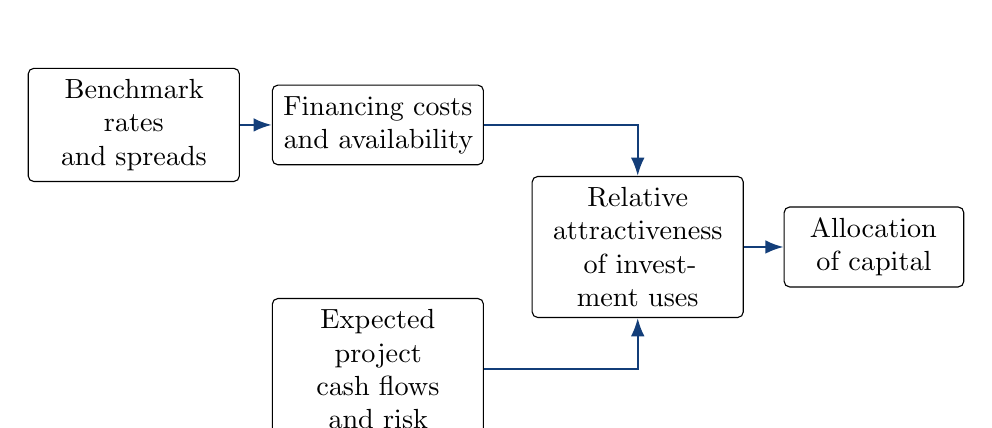
\begin{tikzpicture}[
  >=Latex,
  box/.style={
    draw,
    rounded corners=2pt,
    align=center,
    text width=2.4cm,
    minimum height=0.9cm,
    inner sep=4pt
  },
  box1/.style={
    draw,
    rounded corners=2pt,
    align=center,
    text width=2.0cm,
    minimum height=0.9cm,
    inner sep=4pt
  },
  flow/.style={
    -Latex,
    line width=0.8pt,
    FinanceBlue
  }
]

% Financing conditions
\node[box] (rates) at (-0.6,1.6)
  {Benchmark rates\\and spreads};

\node[box] (finance) at (2.5,1.6)
  {Financing costs\\and availability};

% Investment fundamentals
\node[box] (projects) at (2.5,-1.5)
  {Expected project\\cash flows and risk};

% Investment choice
\node[box] (ranking) at (5.8,0.05)
  {Relative attractiveness\\of investment uses};

\node[box1] (allocation) at (8.8,0.05)
  {Allocation\\of capital};

% Arrows
\draw[flow] (rates.east) -- (finance.west);

\draw[flow] (finance.east) -| (ranking.north);

\draw[flow] (projects.east) -| (ranking.south);

\draw[flow] (ranking.east) -- (allocation.west);

\end{tikzpicture}

\caption{Financing Conditions and the Allocation of Capital}
\label{fig:ch6-capital-allocation}
\end{figure}

Figure~\ref{fig:ch6-capital-allocation} summarizes these
relationships. Benchmark rates and spreads affect
financing costs and the availability of external funds,
while expected project cash flows and risk shape the
prospective returns on alternative investment uses.
Because financing conditions differ across borrowers,
a common change in market interest rates need not affect
all projects equally. Interest-rate changes can therefore
alter not only aggregate investment but also the
allocation of capital across borrowers and activities.

\subsection{Required Returns and Capital Allocation}

Market interest rates provide benchmarks for required returns. The required return on a particular borrower or financial claim can be expressed as a benchmark rate plus a spread reflecting borrower- or instrument-specific characteristics. Differences in credit risk, liquidity, collateral, information quality, and contractual terms can produce different required returns even when the benchmark rate is the same.

Changes in benchmark rates and spreads can alter financing conditions unevenly across borrowers. Table~\ref{tab:ch6-borrower-financing-rates} illustrates this distinction.

\begin{table}[H]

\centering

\caption{Changes in benchmark rates, spreads, and financing rates}

\label{tab:ch6-borrower-financing-rates}

\begin{tabular}{@{}lccc@{}}

\toprule

\textbf{Borrower} &
\textbf{Benchmark rate} &
\textbf{Spread} &
\textbf{Financing rate} \\

\midrule

Lower-risk borrower
& 3.0\% $\rightarrow$ 4.0\%
& 1.0\% $\rightarrow$ 1.0\%
& 4.0\% $\rightarrow$ 5.0\% \\

Higher-risk borrower
& 3.0\% $\rightarrow$ 4.0\%& 3.0\% $\rightarrow$ 4.0\%
& 6.0\% $\rightarrow$ 8.0\% \\

\bottomrule

\end{tabular}

\end{table}

Both borrowers face the same increase in the benchmark rate, but the widening spread produces a larger increase in the financing rate of the higher-risk borrower. Its borrowing and investment may respond more strongly to the deterioration in financing conditions.

These differences in financing costs affect capital allocation. A rise in benchmark rates increases the general opportunity cost of funds, while changes in spreads alter relative financing costs across borrowers. When spreads widen unevenly, capital may shift toward borrowers facing more favorable financing conditions. Interest rates influence both aggregate investment and its allocation across borrowers and activities.

%========================================================
% Summary
%========================================================

\TailModule{summary}{Summary}

An interest rate is the price at which purchasing power today is exchanged for purchasing power in the future. It represents a return to lenders, a cost to borrowers, and a benchmark for investment decisions, linking cash flows across dates. Interest-rate quotations depend on the time horizon and compounding convention. Effective annual rates provide a common basis for comparing rates quoted with different compounding frequencies or under continuous compounding. The distinction between nominal and real rates separates changes in money values from changes in purchasing power.

Observed interest rates reflect several economic forces. Saving and investment affect the supply of and demand for financing, expected inflation influences nominal rates, monetary conditions affect short-term rates and expectations, and differences in risk and liquidity create spreads across instruments. A higher observed rate does not, by itself, identify a single underlying cause.

The term structure describes how interest rates vary across maturities. Spot rates discount cash flows at specific future dates, while forward rates apply to future periods and can be derived from current spot rates under no-arbitrage conditions. The expectations hypothesis links longer-term rates to expected future short-term rates. Market segmentation, maturity preferences, and maturity-specific supply and demand can also affect rates across maturities. Modern term-structure analysis separates longer-term rates into an expected short-rate component and a time-varying term premium.

Interest rates influence both the volume and the allocation of capital. Changes in benchmark rates alter the general opportunity cost of funds, while differences in spreads generate different financing conditions across borrowers. Higher required returns tend to reduce financing for marginal investment opportunities, but the effects need not be uniform across borrowers or uses of capital. Financial markets allocate capital through relative financing costs as well as through the general level of interest rates.

%========================================================
% Key Terms
%========================================================

\TailModule{keyterms}{Key Terms}

Interest rate; opportunity cost of funds; simple interest; compound interest; compounding frequency; nominal annual rate; effective annual rate; continuous compounding; nominal interest rate; real interest rate; expected inflation; Fisher relation; policy rate; benchmark rate; credit spread; risk premium; term structure of interest rates; spot rate; forward rate; yield curve; expectations hypothesis; market segmentation; preferred habitat; term premium; required return; capital allocation.

%========================================================
% Financial AI Lab
%========================================================

\TailModule{aiprompt}{Financial AI Lab}

\textbf{Lab 1: Audit an Interest-Rate Comparison}

Ask an AI system to compare three interest-rate quotations that use different compounding conventions, including at least one continuously compounded rate. Require the AI to place the rates on a common time and compounding basis and to state all assumptions used in the conversion.

Audit the answer independently. Check whether the time horizons are comparable, whether nominal and effective rates are distinguished correctly, and whether the ranking of the alternatives changes after conversion.

Extend the exercise by introducing expected inflation. Ask the AI to distinguish nominal and real interest rates and to apply the Fisher relation. Check whether it distinguishes an expected real rate based on expected inflation from a realized real rate based on actual inflation.

\textbf{Lab 2: Audit a Yield-Curve Interpretation}

Ask an AI system to interpret an upward-sloping yield curve and explain what it implies about future short-term interest rates.

Examine whether the response treats forward rates as certain forecasts or attributes the slope entirely to expectations of rising short-term rates. Revise the interpretation using the distinction between expected future short-term rates and term premia, together with maturity-specific supply and demand conditions.

Repeat the exercise for a flat or inverted yield curve. Determine which conclusions follow from the observed curve and which require additional assumptions about expectations or term premia.

%========================================================
% Discussion Questions
%========================================================

\TailModule{questions}{Discussion Questions}

\begin{enumerate}

\item Why is the interest rate an opportunity cost even for a firm that finances an investment entirely with internal funds?

\item Why can two loans with the same quoted annual percentage rate have different effective borrowing costs?

\item How can a central bank reduce its policy rate while the borrowing rate faced by a risky firm rises?

\item Why should a forward rate not automatically be interpreted as the market's unbiased forecast of a future short-term rate?

\item Why can the same increase in a benchmark interest rate affect investment differently across borrowers?

\end{enumerate}

%========================================================
% Applied Problems
%========================================================

\TailModule{appprobs}{Applied Problems}

\begin{enumerate}

\item \textbf{Compounding and effective rates.}

A bank quotes a nominal annual deposit rate of 5.4\% compounded monthly. A second deposit pays 5.5\% with annual compounding. A third deposit quotes a continuously compounded annual rate of 5.35\%.

\begin{enumerate}

\item Calculate the monthly rate on the first deposit.

\item Calculate the effective annual rate on the first deposit.

\item Calculate the effective annual rate on the continuously compounded deposit.

\item Compare the effective annual returns on all three deposits.

\item Rank the three deposits from highest to lowest effective annual return.

\end{enumerate}


\item \textbf{Nominal and real returns.}

An investor earns a nominal return of 7.5\% over one year.

\begin{enumerate}

\item Calculate the exact real return if inflation is 2.5\%.

\item Calculate the approximate real return using the Fisher approximation.

\item Recalculate both measures if inflation is 6\%.

\item Explain why the approximation becomes less accurate as the rates increase.

\end{enumerate}


\item \textbf{Spot and forward rates.}

The one-year spot rate is 3.0\% and the two-year spot rate is 4.2\%, with annual compounding.

\begin{enumerate}

\item Calculate the one-year forward rate beginning one year from today.

\item Verify that investing for two years at the two-year spot rate produces the same final value as investing for one year at the one-year spot rate and then at the implied forward rate.

\item Explain why the forward rate need not equal the expected future one-year short rate.

\end{enumerate}


\item \textbf{Expectations and term premia.}

The current one-year rate is 3\%. The expected one-year short rates for years 2 and 3 are 4\% and 5\%.

\begin{enumerate}

\item Under the expectations hypothesis, calculate the approximate three-year spot rate.

\item Suppose the three-year term premium is 0.6 percentage point. What approximate three-year spot rate would result?

\item Explain why observing the three-year spot rate alone does not identify expected future short-term rates.

\end{enumerate}


\item \textbf{Benchmark rates, spreads, and capital allocation.}

Two borrowers initially face the same benchmark interest rate of 3.0\%. The lower-risk borrower has a credit spread of 1.0\%, while the higher-risk borrower has a spread of 3.0\%.

The benchmark rate subsequently rises to 4.0\%. The lower-risk borrower's spread remains unchanged, while the higher-risk borrower's spread widens to 4.0\%.

\begin{enumerate}

\item Calculate the initial financing rate for each borrower.

\item Calculate the new financing rate for each borrower.

\item Which borrower experiences the larger increase in financing cost?

\item Explain how the change in relative financing conditions can affect the allocation of capital across borrowers.

\item Explain why a change in the benchmark rate alone is insufficient to determine how financing conditions change across the market.

\end{enumerate}

\end{enumerate}

%========================================================
% Data Application
%========================================================

\TailModule{dataapp}{Data Application}

\textbf{Reading the Yield Curve}

Obtain government-security yields across several maturities for a selected date from an authoritative data source. For China, suitable data include ChinaBond yield-curve data published by China Central Depository \& Clearing Co., Ltd. For an international comparison, use data from a central bank, treasury, government debt-management office, or another authoritative market source.

Construct a yield curve using maturities that are as comparable as possible in credit quality, instrument type, and yield definition.

Describe whether the curve is upward sloping, approximately flat, inverted, or non-monotonic. Consider three possible contributors to the observed pattern:

\begin{itemize}

\item expectations of future short-term rates;

\item term premia;

\item maturity-specific supply, demand, or liquidity conditions.

\end{itemize}

The observed curve alone does not identify expected future policy rates. Explain what assumptions about term premia and other maturity-specific effects would be required for such an interpretation.

If data for two dates are available, compare how the curve changed. Identify whether the change was concentrated at short maturities, long maturities, or across the curve, and discuss what additional evidence would be needed before assigning a causal interpretation.

Report the observation dates, maturities, yield definitions, and primary data source.

%========================================================
% Further Reading
%========================================================

\TailModule{furtherread}{Further Reading}

\begin{itemize}

\item Fisher, Irving (1930), \emph{The Theory of Interest: As Determined by Impatience to Spend Income and Opportunity to Invest It}, The Macmillan Company.

\item Hicks, John R. (1939), \emph{Value and Capital: An Inquiry into Some Fundamental Principles of Economic Theory}, Clarendon Press.

\item Lutz, Friedrich A. (1940), ``The Structure of Interest Rates,'' \emph{Quarterly Journal of Economics}, 55(1), 36--63.

\item Modigliani, Franco, and Richard Sutch (1966), ``Innovations in Interest Rate Policy,'' \emph{American Economic Review}, 56(1/2), 178--197.

\item Campbell, John Y., Andrew W. Lo, and A. Craig MacKinlay (1997), \emph{The Econometrics of Financial Markets}, Princeton University Press.

\end{itemize}

\ChapterTail{summary,keyterms,aiprompt,questions,appprobs,dataapp,furtherread}

\chapter{Money Markets and Short-Term Liquidity Contracts}
\label{chap:Money_Markets_and_Short_Term_Liquidity_Contracts}

\begin{openingcase}[Historical Case Based on Public Information]{When Overnight Funding Suddenly Became Expensive}

In June 2013, China's interbank money market experienced an unusually sharp liquidity squeeze. Short-term repo rates that had generally remained in low single digits rose abruptly, and on 20 June some benchmark overnight and seven-day repo rates reached exceptional intraday levels. Trading activity also contracted as banks became more cautious about lending to one another.

The squeeze emerged in very short-term interbank funding rather than from an obvious deterioration in the long-term value of bank assets. Seasonal cash demands, tax payments, changes in capital flows, and tighter central-bank liquidity conditions coincided with the rise in short-term rates. As uncertainty increased, banks became more cautious about lending to one another, and trading activity weakened.

Why could a market used routinely for day-to-day liquidity adjustment become so strained in such a short period?\footnote{People's Bank of China, \emph{China Monetary Policy Report, Quarter 2, 2013}; and People's Bank of China, \emph{China Financial Market Development Report 2013}.}

\end{openingcase}

\begin{tcolorbox}[
  enhanced,
  colback=FinanceBlue!6,
  colframe=FinanceBlue,
  boxrule=0.6pt,
  sharp corners,
  left=8pt,
  right=8pt,
  top=7pt,
  bottom=7pt,
  before skip=1em,
  after skip=1.6em,
  title=\textbf{Core Questions},
  coltitle=white,
  colbacktitle=FinanceBlue,
  fonttitle=\bfseries,
  attach boxed title to top left={xshift=6pt,yshift=-2mm},
  boxed title style={
    boxrule=0pt,
    sharp corners,
    left=5pt,
    right=5pt,
    top=2pt,
    bottom=2pt
  }
]
\begin{enumerate}[
  leftmargin=*,
  label=\textcolor{FinanceBlue}{\textbf{\arabic*.}},
  itemsep=0.55em,
  topsep=0.2em
]

\item Why do firms and financial institutions need short-term finance even when their underlying activities are long lived?

\item How do unsecured and collateralized money-market contracts redistribute liquidity and determine the terms of short-term funding?

\item How are short-term funding conditions priced, and why can normally liquid money markets become fragile under stress?

\end{enumerate}
\end{tcolorbox}

\section{The Economics of Short-Term Finance}

Short-term finance allows firms and financial institutions to meet payment needs without holding large amounts of idle cash. Its usefulness comes from liquidity and flexibility, but short maturity also creates a need for repeated refinancing.

\subsection{Cash-Flow Timing and Short-Term Funding Needs}

Cash receipts and cash payments do not always occur at
the same time. A solvent firm may nevertheless face a
temporary cash shortfall. Short-term funding bridges
these timing gaps and reduces the amount of idle cash
that participants need to hold.

Consider a firm that has an initial cash balance of
RMB 200,000. It must pay RMB 800,000 to employees and
suppliers within one week, but expects to receive
RMB 1 million from a customer in 28 days. The firm's
cash position evolves as follows:

\begin{itemize}
\item At the beginning of the period, the firm has
RMB 200,000 in cash.

\item When the payment falls due on day 7, the firm
faces a cash shortfall of RMB 600,000.

\item On day 28, the customer pays RMB 1 million,
allowing the firm to repay the short-term borrowing
and retain a positive cash balance.
\end{itemize}

The firm therefore needs RMB 600,000 in temporary
financing, even though its expected cash inflows exceed
its scheduled cash outflows over the period. This example
illustrates how differences in the timing of receipts
and payments can create funding needs that are not
apparent from end-of-period cash balances.

Similar timing problems arise in financial institutions.
Banks may face settlement outflows before incoming
payments arrive, while securities dealers may need to
renew overnight financing for securities inventories
held over longer periods. Margin payments and
concentrated payment obligations can also create
temporary funding needs.

A short-term cash shortfall does not necessarily imply
insolvency. Solvency concerns whether the economic
value of assets is sufficient to cover liabilities,
whereas liquidity concerns whether payments can be
made when they fall due. An institution may therefore
be solvent and still face a liquidity shortage if it
cannot convert assets into cash or obtain new funding
in time to meet its payment obligations.
\begin{figure}[H]
\centering
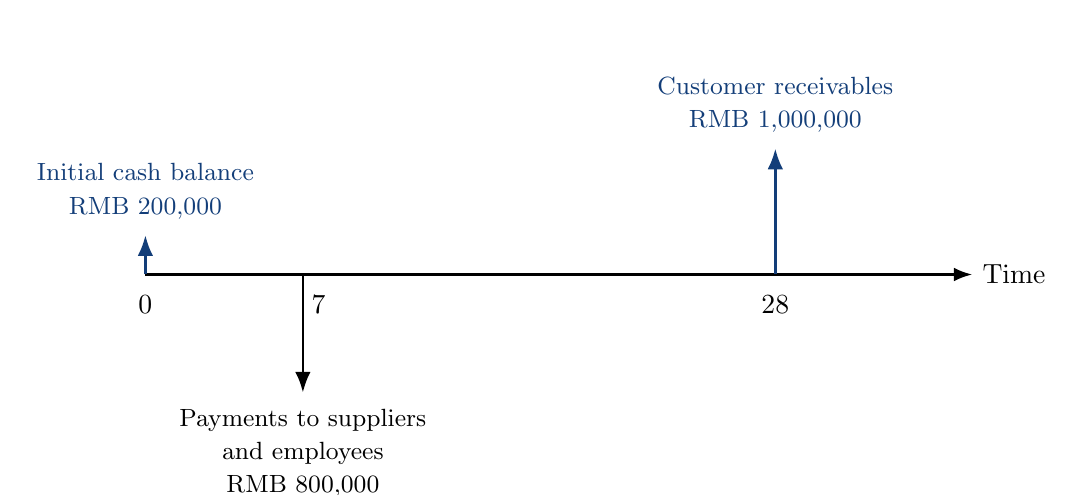
\begin{tikzpicture}[
  >=Latex,
  axis/.style={-Latex, line width=0.8pt},
  inflow/.style={-Latex, line width=1.0pt, FinanceBlue},
  outflow/.style={-Latex, line width=1.0pt}
]

\draw[axis] (0,0) -- (10.5,0) node[right]{Time};

% Tick labels
\node[below=4pt] at (0,0) {0};
\node[below=4pt] at (2.2,0) {7};
\node[below=4pt] at (8,0) {28};

% Initial cash
\draw[inflow] (0,0) -- (0,0.5)
  node[above=2pt, align=center]
   {\small Initial cash balance\\\small RMB 200,000};
% Cash outflow
\draw[outflow] (2,0) -- (2,-1.5)
  node[below=2pt, align=center]
  {\small Payments to suppliers\\\small and employees\\\small RMB 800,000};

% Cash inflow
\draw[inflow] (8,0) -- (8,1.6)
  node[above=2pt, align=center]
  {\small Customer receivables\\\small RMB 1,000,000};

\end{tikzpicture}

\caption{A cash-flow timing gap and the role of short-term finance}
\label{fig:ch7-cash-flow-timing}
\end{figure}

Similar timing problems also arise within the financial
system. One institution may receive more cash than it
needs today, while another faces a temporary deficit.
Money markets redistribute these balances. In doing so,
they allow participants to economize on idle liquidity
and support the settlement of payments and securities
transactions.

The maturity of the funding arrangement affects risk.
If the timing gap is genuinely temporary, short-term
borrowing can match the underlying need closely.
If short-term debt finances an asset that remains
illiquid for years, however, the borrower must refinance
repeatedly. This maturity mismatch creates rollover risk:
the risk that replacement funding will become more
expensive or unavailable when existing funding matures.

\begin{example}{Managing Multiple Cash-Flow Obligations}
{multiple-cash-flow-obligations}

A manufacturing firm begins a 15-day period with a
cash balance of RMB~2 million. During this period,
it faces several payment obligations and expects
customer receipts at different dates. Its projected
cash flows before new financing are summarized below.

\begin{center}
\begin{tabular}{lrr}
\toprule
\textbf{Date} &
\shortstack[c]{\textbf{Cash flow}\\\textbf{(RMB million)}} &
\shortstack[c]{\textbf{Cumulative}\\\textbf{cash balance}} \\
\midrule
Beginning of period & 2.0 & 2.0 \\
Day 2: Supplier payment & -5.0 & -3.0 \\
Day 4: Customer receipt & 1.5 & -1.5 \\
Day 5: Wages and taxes & -1.0 & -2.5 \\
Day 8: Customer receipt & 4.0 & 1.5 \\
Day 10: Transport and interest & -0.5 & 1.0 \\
Day 15: Customer receipt & 2.0 & 3.0 \\
\bottomrule
\end{tabular}
\end{center}

The firm faces its largest cash shortfall on day 2,
when its projected cash balance falls to negative
RMB~3 million. It therefore needs at least RMB~3
million in temporary financing to meet its payment
obligations. Subsequent customer receipts allow the
firm to reduce or repay this borrowing.

The example illustrates why short-term funding
requirements depend on the sequence of cash flows,
not merely on the difference between total receipts
and total payments over a given period. Although
the firm ends the period with a positive cash balance,
it cannot meet all its obligations without temporary
external financing.

A committed credit line or a short-term loan can
bridge this gap. The choice of financing depends on
its availability, cost, maturity, and the reliability
of expected customer payments.

\end{example}

\subsection{Working Capital, Liquidity Management, and Financial Flexibility}

For nonfinancial firms, short-term funding is closely connected to working capital. Operating activity ties funds up in inventory and receivables before cash is collected, while trade credit from suppliers provides a source of short-term financing.

A simplified measure of operating working capital is

\begin{equation*}
OWC=\text{Inventories}+\text{Receivables}-\text{Payables}.
\label{eq:ch7-operating-working-capital}
\end{equation*}

An increase in inventories or receivables absorbs funds, while an increase in payables provides short-term financing. Rapid sales growth can increase short-term financing needs even for a profitable firm if cash must be committed before customers pay.

Liquidity management concerns the assets and funding arrangements used to meet short-term cash needs. Firms may hold cash and marketable securities, maintain committed bank credit, or obtain short-term market funding. The choice among these alternatives reflects a trade-off between liquidity protection and financing cost. Larger liquidity buffers reduce exposure to temporary funding disruptions, but liquid assets generally offer lower returns than productive investment. Committed credit lines provide assured access to funds at a cost, whereas reliance on very short-term market funding increases exposure to rollover risk.

Financial flexibility refers to the capacity to obtain funding or adjust financing arrangements without incurring substantial costs or disrupting investment and operations. It depends not only on current cash holdings but also on unused borrowing capacity, access to alternative funding markets, unencumbered collateral, the maturity structure of liabilities, and borrower creditworthiness. These factors determine the extent to which financing can be raised or restructured when conditions change.

For financial institutions, liquidity management and financial flexibility depend heavily on the composition of assets and access to funding markets. Banks may hold high-quality liquid assets that can be sold or pledged, obtain funding in interbank markets, and access central-bank liquidity against eligible collateral. Securities dealers often finance inventories through repurchase agreements, so their funding capacity depends in part on collateral eligibility and haircuts. Money market funds hold short-term assets, but rapid redemptions can still create liquidity pressure when those assets cannot be sold readily without significant price concessions.

Short-term finance therefore provides flexibility while also creating refinancing dependence. Short maturities allow funding conditions to adjust rapidly, but they also require borrowers to return to lenders or markets more frequently. Maturity determines not only the timing of repayment but also the frequency with which funding is repriced, renewed, or withdrawn.

\begin{tcolorbox}[
    enhanced,
    breakable,
    colback=white,
    colframe=FinanceBlue,
    boxrule=0.7pt,
    sharp corners,
    borderline west={2.2pt}{0pt}{FinanceBlue},
    title=\textbf{Financial Perspective: Short Maturity and Rollover Dependence},
    coltitle=white,
    colbacktitle=FinanceBlue,
    fonttitle=\bfseries,
    before skip=1.2em,
    after skip=1.2em
]

Short-term borrowing can provide flexibility by allowing financing terms to adjust frequently. The same feature, however, increases dependence on refinancing. A lender to a one-day loan commits funds only until maturity and may reprice or decline to renew the loan at the next rollover date. If the underlying funding need continues, the borrower remains exposed to changes in market conditions. Short maturity therefore increases the importance of rollover decisions and concentrates funding risk at refinancing dates.

\end{tcolorbox}

\section{Money Market Contracts and Instruments}

Money-market instruments and contracts are short-term
claims and funding arrangements used to meet temporary
funding needs, manage cash balances, and finance
securities positions. They differ in issuer or
counterparty, collateral, credit exposure, tradability,
and quotation conventions. These differences affect
their pricing, liquidity, and risk.

\subsection{Treasury Bills and Sovereign Short-Term Claims}

Treasury bills are short-term debt securities issued by central governments. They typically make no periodic coupon payments and pay a fixed face value at maturity, with the return arising from the difference between the purchase price and the maturity value.

If a bill with face value \(F\) is purchased for \(P\) and held for \(d\) days until maturity, its holding-period return is

\begin{equation}
HPR=\frac{F-P}{P}.
\label{eq:ch7-tbill-hpr}
\end{equation}

To compare bills with different maturities, the holding-period return can be annualized on a simple-interest basis. The resulting yield depends on the market's quotation convention. A money-market yield based on the purchase price can be written as

\begin{equation}
y_m=\frac{F-P}{P}\frac{D}{d},
\label{eq:ch7-money-market-yield}
\end{equation}
where $D$ denotes the annual day-count basis specified by market convention, commonly 360 or 365.

Some bill markets also use a discount yield based on face value:

\begin{equation}
y_d=\frac{F-P}{F}\frac{D}{d}.
\label{eq:ch7-discount-yield}
\end{equation}

\begin{example}{The Quotation Convention Changes the Reported Yield}{tbill-quotation-convention}

A 91-day bill with face value 100 sells for 98.80. Using a 360-day basis, the holding-period return is

\[
HPR=\frac{100-98.80}{98.80}=1.2146\%.
\]

The annualized money-market yield is

\[
y_m=\frac{1.20}{98.80}\frac{360}{91}=4.805\%,
\]
while the discount yield is

\[
y_d=\frac{1.20}{100}\frac{360}{91}=4.747\%.
\]

Both yields refer to the same underlying cash flow. Their numerical difference arises solely from the quotation convention.

\end{example}

Treasury bills are the most common form of short-term sovereign debt, although the precise instruments, maturities, and issuance conventions differ across countries.

Sovereign short-term securities play several roles beyond government financing. When credit risk is low and secondary-market liquidity is high, they provide instruments for temporary cash investment, collateral for secured funding, and benchmarks for the pricing of other short-term claims.

Low credit risk does not imply a risk-free market price over every holding period. A bill sold before maturity can change in price as market rates change. Settlement, market liquidity, and sovereign credit conditions can also matter. Their short maturity generally results in lower interest-rate sensitivity than that of otherwise similar longer-maturity fixed-rate securities.

\subsection{Commercial Paper and Short-Term Corporate Funding}

Commercial paper (CP) is a short-term, typically unsecured
debt instrument issued by corporations and financial
institutions to meet short-term funding needs. Investors
rely primarily on the issuer's creditworthiness and
liquidity position. Commercial paper can be issued on
a discount basis or an interest-bearing basis. Discount
paper is issued below face value and repaid at face
value at maturity, whereas interest-bearing paper pays
stated interest in addition to principal.

The two structures differ in how investors receive
their returns. For discount paper, the return is
generated by the difference between the purchase price
and the face value. For interest-bearing paper, the
return comes from the stated interest payment.

\begin{example}{Discount and Interest-Bearing Commercial Paper}
{commercial-paper-payment-structures}

Consider two 90-day commercial paper issues, each with
a principal or face value of RMB~10 million. Assume
a 360-day year for interest calculations.

\textbf{Discount commercial paper.}

Suppose the paper is issued at RMB~9.85 million and
redeemed at its face value of RMB~10 million after
90 days. The investor earns RMB~0.15 million. The
annualized discount rate is

\[
d=\frac{10-9.85}{10}\times\frac{360}{90}
=6\%.
\]

The corresponding simple annualized investment yield,
calculated using the purchase price as the denominator,
is

\[
y=\frac{10-9.85}{9.85}\times\frac{360}{90}
\approx 6.09\%.
\]

\textbf{Interest-bearing commercial paper.}

Suppose the paper is issued at par with an annual
interest rate of 6\%. Interest payable at maturity is

\[
I=10\times 6\%\times\frac{90}{360}
=0.15\text{ million}.
\]

The investor receives RMB~10.15 million at maturity,
consisting of principal and interest. Its simple
annualized yield is 6\%.

The example illustrates that discount rates and
investment yields are not identical. The discount
rate is calculated using face value, whereas the
investment yield is calculated using the purchase
price. Interest-bearing paper, when issued at par,
expresses its return through the stated interest rate.

Although both quoted rates are 6\%, the discount
paper provides a slightly higher investment yield
because its discount rate is calculated using face
value rather than the purchase price.

\end{example}

Investors require compensation for the time value
of money and for the credit and liquidity risks
associated with the issuer. The required yield
therefore reflects the benchmark rate for a comparable
maturity and a spread associated with issuer-specific
credit and liquidity conditions.

For issuers with strong credit quality, commercial
paper provides direct access to short-term market
funding and may offer a lower-cost alternative to
bank borrowing. However, reliance on repeated issuance
creates rollover risk. A firm that relies on 30-day
paper must repay maturing claims from available cash
or obtain new financing at each maturity. If perceived
credit quality deteriorates or investor demand weakens,
spreads may widen and access to new issuance may become
restricted. Firms therefore often support commercial
paper programs with committed bank credit lines or
liquidity reserves. Rollover risk can arise even when
the issuer remains solvent.

A related form of short-term market funding is
asset-backed commercial paper (ABCP). Unlike ordinary
corporate commercial paper, ABCP is issued by a
special-purpose vehicle backed by pools of financial
assets, such as receivables or loans. The program may
also benefit from liquidity facilities or credit
enhancement provided by sponsors or other institutions.

\subsection{Certificates of Deposit and Bank Funding}

A certificate of deposit is a bank liability that promises repayment of principal, usually with interest, at a specified maturity. A negotiable certificate of deposit can be transferred before maturity, allowing the original investor to obtain liquidity by selling the claim rather than asking the issuing bank to repay it early.

From the bank's perspective, negotiable CDs are an instrument of liability management. They allow a bank to raise funds at market-determined rates rather than relying entirely on deposits generated through its retail customer base. The rate offered reflects the maturity of the claim, market liquidity, the bank's credit quality, and the supply of alternative short-term investments.

Tradability changes how investors obtain liquidity before maturity. A nontransferable time deposit generally requires the depositor to retain the claim until maturity or seek early withdrawal from the bank. A negotiable CD can instead be sold in the secondary market, although its price may vary with market interest rates and the perceived credit quality of the issuing bank.

\begin{table}[H]
\centering
\caption{Time deposits and negotiable certificates of deposit}
\label{tab:ch7-cd-comparison}

\begin{tabularx}{\textwidth}{lXX}
\toprule
 & \textbf{Nontransferable Time Deposit} & \textbf{Negotiable CD} \\
\midrule

Transferability
& Generally nontransferable
& Transferable in the secondary market \\

Liquidity before maturity
& Usually requires early withdrawal or other arrangements with the bank
& Can be obtained by selling the claim \\

Investor exposure
& Primarily to the issuing bank
& To the issuing bank, with market-price risk before maturity \\

Funding role for the bank
& Deposit funding
& Market-based wholesale funding \\

\bottomrule
\end{tabularx}
\end{table}

China's interbank certificates of deposit provide an
important example of market-based bank funding.
Introduced under the People's Bank of China's
2013 provisional rules, these book-entry time-deposit
certificates are issued by eligible deposit-taking
institutions in the national interbank market.
Their issuance rates are market based, and publicly
issued certificates can be traded in the secondary
market. They provide banks with an additional source
of wholesale funding and investors with a transferable
claim on the issuing institution.

\subsection{Interbank Loans and Overnight Unsecured Funding}

Banks routinely receive and make payments on behalf of customers. These flows create temporary differences in liquidity positions. Interbank lending allows institutions with surplus funds to lend to those with short-term deficits.

An unsecured interbank loan is a direct claim on the borrowing bank. No specific collateral supports repayment, so the lender relies on the borrower's creditworthiness and on bilateral or market-wide credit limits. The interest rate therefore reflects both general liquidity conditions and counterparty credit risk.

Overnight maturities play a central role in the rapid
redistribution of liquidity. A bank that experiences
an unexpected settlement outflow today may borrow
overnight and repay after incoming funds arrive the
next day. Funding with maturities of several days or
months allows liquidity to be secured for longer
periods but extends the lender's exposure to the
borrower.

The unsecured nature of the claim becomes more
consequential during periods of stress. A bank that
is uncertain about a counterparty's creditworthiness
can refuse to lend even when it has cash available.
If many institutions behave similarly, the market
can become segmented across counterparties: liquidity
remains in the system but is not redistributed toward
institutions that need it.

Credit limits matter alongside the market interest rate. An offered rate can rise substantially without inducing additional lending if lenders are unwilling to increase unsecured exposure. In such circumstances, the quantity of available credit and the identity of counterparties become as important as the quoted price.

\subsection{Repurchase Agreements and Collateralized Funding}

A repurchase agreement, or repo, is a short-term funding contract in which one party receives cash against securities and agrees to reverse the transaction later at a specified repurchase price. Economically, a repo functions as collateralized short-term funding, although its legal structure varies across markets.

From the perspective of the cash borrower, the transaction is a repo. From the perspective of the cash lender, the same transaction is a reverse repo. Let collateral with market value $V_0$ support a repo. If the lender applies haircut $h$, the cash advanced is

\begin{equation}
C_0=(1-h)V_0.
\label{eq:ch7-repo-cash-haircut}
\end{equation}

The haircut provides a buffer against declines in collateral value and the costs of liquidation if the borrower defaults. If the repo lasts for fraction $\tau$ of a year and the repo rate is $r_{repo}$, the repurchase payment is

\begin{equation}
C_T=C_0(1+r_{repo}\tau),
\label{eq:ch7-repo-repurchase-payment}
\end{equation}
under a simple-interest convention for the repo period.

\begin{example}{Repo Funding and the Haircut}{repo-funding-haircut}

A dealer holds government securities with a market value of RMB~100 million and finances them through a one-week repo. The cash lender applies a 2\% haircut.

The cash advanced is

\[
C_0=(1-0.02)\times100=98
\]

million renminbi. If the annualized repo rate is 2.5\%  and the market uses a 365-day basis, the repurchase payment after seven days is

\[
C_T=98\times\left(1+0.025\times\frac{7}{365}\right)
\approx 98.047
\]
million renminbi.

The haircut and the repo rate perform different functions. The repo rate is the price of the cash funding; the haircut determines how much cash is advanced relative to the collateral value.

\end{example}

Collateral can reduce the lender's exposure to loss. The collateral price can fall, the security may become difficult to liquidate, or legal and operational problems can delay access to it. Repo contracts commonly use collateral eligibility rules, valuation procedures, haircuts, and margin arrangements.

When collateral values change during the life of a repo, margin adjustments may require additional cash or securities to maintain the agreed level of protection. This mark-to-market mechanism protects the lender but can create liquidity pressure for the borrower when collateral values decline.

Repos are central to securities-market intermediation by allowing dealers and other institutions to finance inventories of bonds and other eligible securities. They also connect the money market to the bond market: the value and liquidity of a security affect its usefulness as collateral, while the availability and cost of repo funding affect the willingness of intermediaries to hold the security.

Table~\ref{tab:ch7-money-market-instruments} summarizes the main contractual differences among the instruments discussed in this section.

\begin{table}[H]
\centering
\caption{Selected Money-Market Instruments and Their Contractual Structure}
\label{tab:ch7-money-market-instruments}

\begin{tabularx}{\textwidth}{
@{}
>{\raggedright\arraybackslash
\hyphenpenalty=10000
\exhyphenpenalty=10000}p{2.3cm}
>{\raggedright\arraybackslash
\hyphenpenalty=10000
\exhyphenpenalty=10000}p{2.5cm}
>{\raggedright\arraybackslash
\hyphenpenalty=10000
\exhyphenpenalty=10000}p{2.6cm}
Y
@{}
}

\toprule

\textbf{Instrument}
&
\makecell[l]{\textbf{Typical issuer}\\\textbf{or borrower}}
&
\makecell[l]{\textbf{Collateral}\\\textbf{or credit basis}}
&
\makecell[l]{\textbf{Main economic role and risk}}
\\

\midrule

Treasury bill
& Central government
& Sovereign obligation; typically unsecured
& Short-term government funding and liquid investment; low credit risk in high-quality sovereign markets, with market-price risk before maturity
\\

Commercial paper
& Corporation or financial institution
& Typically unsecured; issuer credit
& Flexible short-term market funding; issuer credit and rollover risk
\\

Negotiable CD
& Bank
& Bank deposit obligation; typically unsecured
& Wholesale bank funding and a transferable bank claim; bank credit and rollover risk
\\

Interbank loan
& Bank or other financial institution
& Typically unsecured counterparty credit
& Short-term liquidity redistribution; counterparty credit and rollover risk
\\

Repo
& Dealer, bank, fund, or other participant
& Collateralized under a sale-and-repurchase agreement
& Securities financing and liquidity management; collateral valuation, haircut, counterparty, and rollover risk
\\

Asset-backed commercial paper
& Special-purpose vehicle
& Asset pools, often with liquidity or credit support
& Asset-backed short-term funding; underlying asset quality, liquidity, and rollover risk
\\

\bottomrule
\end{tabularx}
\end{table}

\section{Money Market Architecture and Pricing}

Money-market prices are formed through interactions among borrowers, cash investors, banks, dealers, and investment funds within the trading and settlement infrastructure of the market. Contractual terms determine the cash flows of an instrument, while market architecture affects access to funding, the redistribution of liquidity, price discovery and benchmark formation, and the execution and settlement of transactions.

\subsection{Banks, Dealers, and Money Market Funds}

Banks act as both borrowers and lenders in the money market. They borrow to manage settlement needs and short-term balance-sheet funding, and they lend when they have temporary surplus liquidity. Their activities connect short-term funding markets with the payment system and the broader banking system.

Securities dealers connect short-term funding with trading in bonds and other securities. A dealer that holds securities in inventory may finance part of the position through repo. This balance-sheet capacity supports secondary-market liquidity by allowing dealers to hold inventories and provide immediacy to buyers and sellers. The cost and availability of repo funding affect the dealer's willingness to make markets.

Money market funds pool investor cash and invest primarily in short-maturity, high-quality instruments. They provide households, firms, and institutions with diversified access to money-market assets while channeling cash toward governments, banks, corporations, and dealers. The fund's portfolio can include government bills, repos, commercial paper, and certificates of deposit, subject to the rules applying to the fund and jurisdiction.

The structure of money market funds creates an
important distinction between asset liquidity and
investor liquidity. Investors may expect to redeem
fund shares on short notice, while some portfolio
assets may be difficult to sell quickly during
periods of market stress.A fund that experiences large redemptions can respond by using cash and proceeds from maturing securities, selling assets, or reducing new purchases. These actions transmit investor withdrawals into the markets used by short-term borrowers.

\begin{figure}[H]
\centering
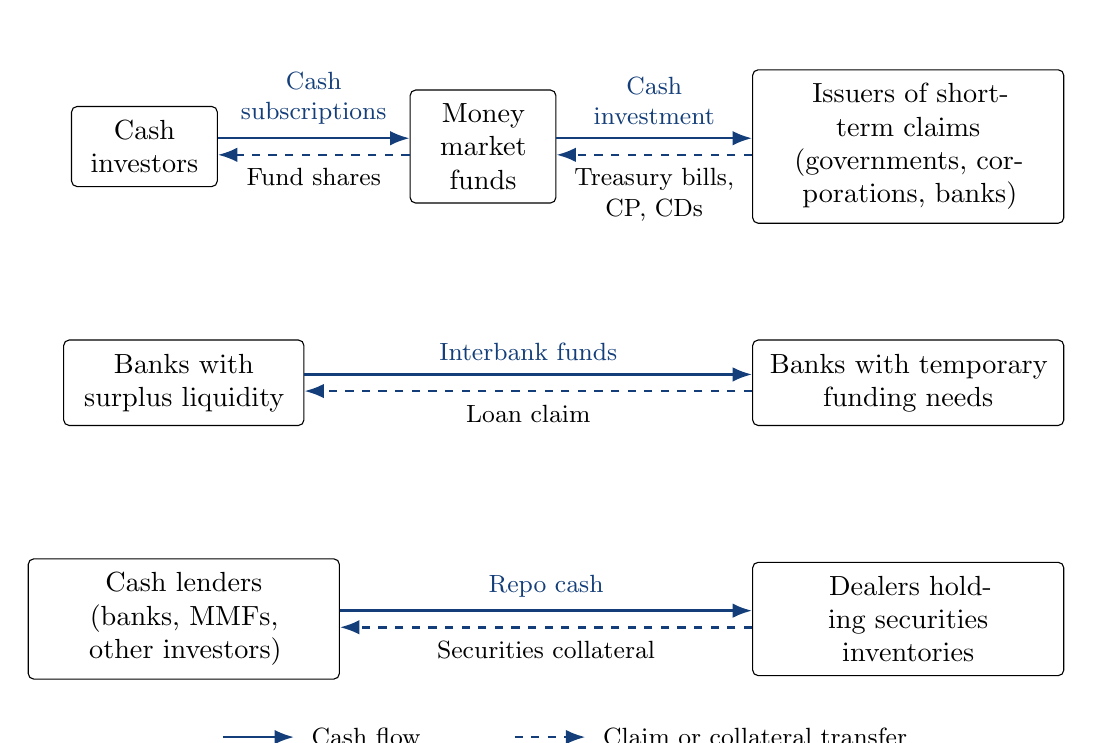
\begin{tikzpicture}[
  >=Latex,
  box/.style={
    draw,
    rounded corners=2pt,
    align=center,
    minimum height=1.0cm,
    text width=2.7cm,
    inner sep=5pt
  },
  widebox/.style={
    draw,
    rounded corners=2pt,
    align=center,
    minimum height=1.0cm,
    text width=3.6cm,
    inner sep=5pt
  },
  fundbox/.style={
    draw,
    rounded corners=2pt,
    align=center,
    minimum height=1.0cm,
    text width=1.5cm,
    inner sep=5pt
  },
  flow/.style={
    -Latex,
    line width=0.9pt,
    FinanceBlue
  },
  claim/.style={
    -Latex,
    dashed,
    line width=0.9pt,
    FinanceBlue
  },
abovelab/.style={
  font=\small,
  text=FinanceBlue,
  fill=white,
  align=center,
  fill=white,
  inner sep=1.5pt
},
  belowlab/.style={
    font=\small,
    text=black,
    fill=white,
    align=center,
    inner sep=1.5pt
  }
]

% =================================================
% Top row: Money market funds
% =================================================

\node[fundbox] (inv) at (-0.5,3.0)
  {Cash investors};

\node[fundbox] (mmf) at (3.8,3.0)
  {Money market\\funds};

\node[widebox] (iss) at (9.2,3.0)
  {Issuers of short-term claims\\
   (governments, corporations, banks)};

% Investor subscriptions and fund shares
\draw[flow]
  ([yshift=3pt]inv.east) --
  node[abovelab, midway, above=3pt] {Cash\\subscriptions}
  ([yshift=3pt]mmf.west);

\draw[claim]
  ([yshift=-3pt]mmf.west) --
  node[belowlab, midway, below=3pt] {Fund shares}
  ([yshift=-3pt]inv.east);

% MMF investment in short-term claims
\draw[flow]
  ([yshift=3pt]mmf.east) --
  node[abovelab, midway, above=3pt] {Cash\\investment}
  ([yshift=3pt]iss.west);

\draw[claim]
  ([yshift=-3pt]iss.west) --
  node[belowlab, midway, below=3pt]
  {Treasury bills,\\ CP, CDs}
  ([yshift=-3pt]mmf.east);


% =================================================
% Middle row: Interbank lending
% =================================================

\node[box] (bank1) at (0,0)
  {Banks with\\surplus liquidity};

\node[widebox] (bank2) at (9.2,0)
  {Banks with temporary\\funding needs};

% Cash and loan claim
\draw[flow]
  ([yshift=3pt]bank1.east) --
  node[abovelab, midway, above=3pt]
  {Interbank funds}
  ([yshift=3pt]bank2.west);

\draw[claim]
  ([yshift=-3pt]bank2.west) --
  node[belowlab, midway, below=3pt]
  {Loan claim}
  ([yshift=-3pt]bank1.east);


% =================================================
% Bottom row: Repo financing
% =================================================

\node[widebox] (cashl) at (0,-3.0)
  {Cash lenders\\(banks, MMFs, other investors)};

\node[widebox] (dealer) at (9.2,-3.0)
  {Dealers holding securities\\inventories};

% Repo cash and collateral
\draw[flow]
  ([yshift=3pt]cashl.east) --
  node[abovelab, midway, above=3pt]
  {Repo cash}
  ([yshift=3pt]dealer.west);

\draw[claim]
  ([yshift=-3pt]dealer.west) --
  node[belowlab, midway, below=3pt]
  {Securities collateral}
  ([yshift=-3pt]cashl.east);


% =================================================
% Legend
% =================================================

\draw[flow] (0.5,-4.5) -- (1.4,-4.5);
\node[anchor=west, draw=none] at (1.5,-4.5)
  {\small Cash flow};

\draw[claim] (4.2,-4.5) -- (5.1,-4.5);
\node[anchor=west, draw=none] at (5.2,-4.5)
  {\small Claim or collateral transfer};

\end{tikzpicture}

\caption{Institutional Channels of Money Market Funding}
\label{fig:ch7-money-market-channels}
\end{figure}

The figure is schematic. Banks can appear on both the lending and borrowing sides of the market, while money market funds and dealers perform different intermediation functions. The purpose is to show how short-term funds move through several institutional channels.

\subsection{Benchmark Rates, Spreads, and Price Discovery}

Central banks influence money-market conditions through
the supply of settlement balances, open-market operations,
and liquidity facilities. These operations affect
very short-term interest rates and the overall availability
of funding. Rates on individual instruments may nevertheless
differ because of counterparty credit risk, collateral
conditions, market segmentation, and institution-specific
funding conditions.

Money-market contracts are frequently priced relative
to benchmark rates. A useful benchmark should represent
a clearly defined market segment, be based on reliable
information, and be supported by a transparent methodology
and appropriate governance. Its economic meaning depends
on the underlying transactions and the method used to
construct the rate.

Benchmarks differ in both the type of funding they measure
and the way they are constructed. One distinction concerns
whether funding is secured or unsecured. Secured rates
reflect funding transactions backed by collateral, with
the resulting rates affected by collateral quality and
availability. Unsecured rates reflect borrowing without
collateral and more directly incorporate counterparty
credit conditions. Another distinction concerns the
method of rate formation. Transaction-based benchmarks
are derived from eligible market transactions, whereas
quotation-based benchmarks rely on rates submitted by
selected market participants.

China's money market illustrates these differences.
The Shanghai Interbank Offered Rate (Shibor) is a
quotation-based unsecured benchmark derived from
submissions by a panel of banks and published across
several maturities. By contrast, the Depository-Institutions
Repo Rate (DR) is a transaction-based secured rate based
on pledged repo transactions among depository institutions
using interest-rate bonds as collateral. DR007, the
seven-day rate, is widely used as an indicator of
banking-system liquidity and as a reference for
money-market pricing.

International benchmark reform has increased the use
of transaction-based overnight rates. SOFR in the
United States is based on secured Treasury repo
transactions, whereas SONIA in the United Kingdom
and €STR in the euro area are based on unsecured
overnight transactions.

The main characteristics of these benchmarks are
summarized in Table~\ref{tab:ch7-benchmark-comparison}.

\begin{table}[H]
\centering
\caption{Selected Money-Market Benchmarks and Their Characteristics}
\label{tab:ch7-benchmark-comparison}

\begin{tabularx}{\textwidth}{
@{}
>{\raggedright\arraybackslash}p{1.7cm}
>{\raggedright\arraybackslash}p{3.2cm}
>{\raggedright\arraybackslash}p{2.0cm}
Y
@{}
}

\toprule

\textbf{Benchmark}
&
\textbf{Underlying market}
&
\textbf{Funding basis}
&
\textbf{Rate formation}
\\

\midrule

Shibor
& RMB interbank funding
& Unsecured
& Bank panel quotations
\\

DR007
& Seven-day interbank pledged repo
& Secured
& Actual transaction-weighted rate
\\

SOFR
& Overnight US Treasury repo
& Secured
& Transaction-based volume-weighted median
\\

SONIA
& Overnight sterling deposits
& Unsecured
& Transaction-based trimmed mean
\\

€STR
& Overnight euro wholesale funding
& Unsecured
& Transaction-based calculation
\\

\bottomrule
\end{tabularx}
\end{table}

For a short-term instrument and a benchmark of comparable
maturity and market characteristics, the spread is

\begin{equation}
s_i=r_i-r_b.
\label{eq:ch7-money-market-spread}
\end{equation}
where $r_i$ denotes the rate on a short-term instrument and $r_b$ an appropriate benchmark.

A widening spread may reflect greater credit risk,
lower market liquidity, tighter balance-sheet constraints,
or weaker demand for the instrument. The same observed
spread can therefore arise from different underlying
conditions.

Price discovery occurs as borrowers and lenders adjust
rates in response to funding needs, new information,
monetary operations, and trading conditions. The short
maturities and frequent repricing of money-market claims
make very short-term rates particularly sensitive to
changes in funding conditions. Overnight rates may move
sharply around tax or reporting dates, following changes
in central-bank liquidity, or when institutions become
less willing to lend.

Benchmark rates are also used in contracts outside the
money market. Floating-rate loans, bonds, swaps, and
derivatives may reference short-term benchmarks when
determining contractual payments. Money-market price
discovery thus affects the pricing and valuation of a
much broader range of financial claims.

\subsection{Collateral, Clearing, and Settlement}

Collateral provides the lender with an additional
source of recovery beyond the borrower's general
creditworthiness. Its effectiveness depends on three
questions: what assets are eligible, how they are
valued, and how quickly the lender can exercise rights
over them after default.

Government securities and other high-quality marketable securities often serve as money-market collateral. Their values are comparatively transparent, and they can generally be sold or financed more easily than less liquid assets. Other securities may also be eligible, but lenders can apply larger haircuts when price volatility, credit risk, or liquidation costs are greater.

An initial haircut provides a buffer against declines
in collateral value, but this buffer may become
insufficient as market prices change. Repo contracts
may therefore require collateral to be marked to
market daily or intraday. If collateral value falls
below the level required under the agreement, the
borrower may need to provide additional securities
or cash. Such margin calls limit the lender's exposure
but can create liquidity pressure for the borrower,
particularly when collateral prices fall sharply.

Clearing establishes the obligations arising from a
transaction and, where applicable, determines the
amounts to be settled. Settlement completes those
obligations through the transfer of cash and securities.
In a securities transaction, the seller must deliver
the securities and the buyer must make the corresponding
cash payment. If these transfers occur at different
times, either party may be exposed to the risk that
the other fails to fulfill its obligation. Delivery-versus-payment
(DvP) arrangements reduce this principal risk by
linking securities delivery to the corresponding
cash payment.

China's interbank market illustrates the division
between trading services and securities registration,
custody, and settlement. The China Foreign Exchange
Trade System (CFETS), also known as the National
Interbank Funding Center, provides issuance, trading,
and information services for interbank certificates
of deposit. Shanghai Clearing House (SHCH) handles
their registration, custody, and settlement. This
arrangement separates the trading of these instruments
from the institutions responsible for maintaining
ownership records and completing settlement.

These arrangements do not eliminate liquidity risk.
Even valuable collateral may fail to provide timely
funding when settlement is delayed or operational
problems prevent its mobilization. Money-market
liquidity therefore depends not only on the quality
of financial claims but also on the infrastructure
through which they are transferred.
\begin{tcolorbox}[
  enhanced,
  breakable,
  colback=white,
  colframe=FinanceBlue,
  boxrule=0.7pt,
  sharp corners,
  borderline west={2.2pt}{0pt}{FinanceBlue},
  title=\textbf{Financial Perspective: Collateral Must Be Mobilizable},
  coltitle=white,
  colbacktitle=FinanceBlue,
  fonttitle=\bfseries,
  before skip=1.2em,
  after skip=1.2em
]

The value of collateral depends not only on its
credit quality and market price but also on whether
it can be transferred, accepted, and liquidated
when funding is needed. Legal, operational, and
settlement frictions can limit its usefulness as
a source of immediate liquidity.

\end{tcolorbox}

\section{Liquidity Stress in Money Markets}

Money markets can appear highly liquid under normal conditions. Short maturities and regular refinancing allow funds to move readily across institutions. The same features, however, can intensify stress when lenders become unwilling to renew funding. Large volumes of debt may mature within a short period, forcing borrowers to obtain cash before longer-term assets can be sold or mature.

\subsection{Funding Runs and Market Freezes}

A funding run occurs when short-term creditors withdraw
funding, refuse to roll over maturing claims, or shorten
the maturity of new lending. The resulting dynamics
resemble those of a bank run, even when the institution
relies on short-term wholesale funding rather than
deposits. A market freeze occurs when trading or new funding
falls sharply because market participants become
unwilling or unable to transact at prevailing terms.

Suppose a borrower finances long-lived assets with debt
that matures daily or weekly. As long as lenders continue
to renew the debt, the position can be maintained.
Concerns about the quality of the borrower's assets,
the borrower's creditworthiness, or lenders' own
liquidity needs may make lenders less willing to
roll over the funding. The borrower must then obtain cash
as existing claims mature.

To meet these obligations, the borrower may draw on
committed credit, use cash reserves, pledge additional
collateral, or sell assets. If many institutions face
similar funding pressures, these responses can reinforce
one another. Asset sales may depress market prices,
while increased demand for liquidity puts further
pressure on funding conditions. Falling asset prices
can also weaken balance sheets and reduce collateral
values, further increasing funding pressure. The process
can become self-reinforcing:


\begin{figure}[H]
\centering
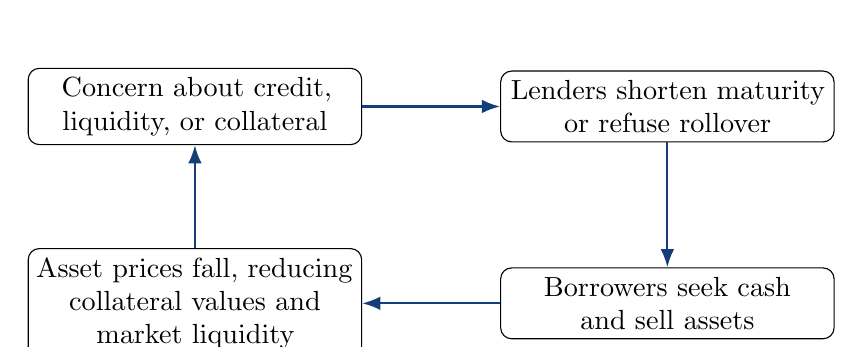
\begin{tikzpicture}[
  >=Latex,
  box/.style={draw, rounded corners, align=center, text width=4.0cm, minimum height=0.9cm},
  flow/.style={-Latex, line width=0.8pt, FinanceBlue}
]

\node[box] (concern) at (0,3.2) {Concern about credit,\\liquidity, or collateral};
\node[box] (roll) at (6.0,3.2) {Lenders shorten maturity\\or refuse rollover};
\node[box] (cash) at (6.0,0.7) {Borrowers seek cash\\and sell assets};
\node[box] (price) at (0,0.7) 
{Asset prices fall, reducing\\collateral values and market liquidity};

\draw[flow] (concern) -- (roll);
\draw[flow] (roll) -- (cash);
\draw[flow] (cash) -- (price);
\draw[flow] (price) -- (concern);

\end{tikzpicture}
\caption{A short-term funding feedback loop}
\label{fig:ch7-funding-run-loop}
\end{figure}

In unsecured markets, uncertainty about borrower quality can reduce lending even when aggregate liquidity remains ample. Institutions may prefer to retain liquidity rather than increase exposure to counterparties whose condition is difficult to assess. Funding stress can affect both price and quantity: spreads may rise while some borrowers lose access to funding altogether.

Similar pressures can arise in commercial-paper markets and money market funds. Investors may shift from commercial paper toward government securities or cash, reducing the funding available to issuers and increasing reliance on committed bank credit lines. Rapid redemptions from money market funds reinforce this process if funds reduce purchases of commercial paper and certificates of deposit or sell assets to meet withdrawals. Stress thus pass from cash investors to short-term borrowers and, in turn, to bank balance sheets.

The June 2013 Chinese interbank episode illustrates these
mechanisms. As funding uncertainty intensified,
institutions became more reluctant to lend, weakening
the redistribution of liquidity across the banking
system. Short-term rates rose sharply before declining
as liquidity conditions and expectations stabilized.

\subsection{Repo Haircuts, Collateral Pressure, and Flight to Quality}

Repo funding conditions depend on both the repo rate and the haircut. The repo rate determines the cost of cash funding, while the haircut determines how much cash can be borrowed against a given amount of collateral.

This distinction becomes especially important during
periods of market stress. Consider a stylized dealer
position financed entirely with repo borrowing and
the dealer's own funds. Let $V$ denote the market
value of the securities and $E$ the dealer's own-funds
contribution. Under the standard haircut convention,
a repo haircut $h$ means that the lender advances
$(1-h)V$ against collateral worth $V$. The dealer
must therefore finance the remaining amount with
its own funds:

\begin{equation*}
E=hV.
\label{eq:ch7-haircut-equity}
\end{equation*}

Under this simplified financing structure, the asset-to-equity ratio is

\begin{equation*}
\frac{V}{E}=\frac{1}{h}.
\label{eq:ch7-haircut-leverage}
\end{equation*}

The financing implications become particularly
significant when haircuts rise during periods of
market stress.

\begin{example}{A Haircut Increase Creates a Funding Need}{haircut-funding-need}

A dealer finances securities with market value RMB~100 million through repo. With a 2\% haircut, the lender provides RMB~98 million and the dealer supplies RMB~2 million of its own funding.

If the haircut rises to 5\% while the collateral value remains RMB~100 million, repo funding falls to RMB~95 million. The dealer must provide an additional RMB~3 million of cash or collateral to maintain the same position.

If many dealers face the same change, they may reduce positions or sell securities to release cash. A haircut intended to protect individual lenders can contribute to system-wide deleveraging when it rises simultaneously across the market.

\end{example}

Collateral pressure intensifies when haircuts rise while collateral values fall. The borrower then faces both a lower borrowing capacity against each unit of collateral and a decline in the value of existing collateral. Margin calls may force asset sales into a falling market, reinforcing the interaction between funding liquidity and market liquidity.

The quality of collateral also affects where liquidity
moves. During stress, lenders often become more willing
to accept government securities and less willing to
accept private or less liquid collateral. Investors
similarly shift cash toward claims perceived as safer
and more liquid. This \emph{flight to quality} can lower
yields on high-quality short-term government claims
while spreads on private money-market instruments
widen. It represents a reallocation of liquidity
across assets and counterparties rather than
necessarily a decline in aggregate liquidity.

The interaction among collateral, haircuts, dealer
balance sheets, and market liquidity explains why
repo markets matter beyond their direct participants.
If dealers lose financing capacity, their ability
and willingness to intermediate bond markets can
decline. Lower market liquidity can then increase
price volatility and reduce the value of securities
used as collateral. Lenders may respond by applying
larger haircuts, further tightening financing
conditions.
\begin{tcolorbox}[
  enhanced,
  breakable,
  colback=white,
  colframe=FinanceBlue,
  boxrule=0.7pt,
  sharp corners,
  borderline west={2.2pt}{0pt}{FinanceBlue},
  title=\textbf{Financial Perspective: A Higher Haircut Can Tighten Funding Without a Higher Interest Rate},
  coltitle=white,
  colbacktitle=FinanceBlue,
  fonttitle=\bfseries,
  before skip=1.2em,
  after skip=1.2em
]

A repo rate can remain unchanged while funding
conditions tighten substantially. A higher haircut
reduces the amount of cash that can be raised against
a given quantity of collateral. Borrowers must provide
more of their own funds, pledge additional collateral,
or reduce their positions. Haircuts therefore affect
the quantity of financing available, even when the
quoted repo rate changes little.

\end{tcolorbox}

%========================================================
% Summary
%========================================================

\TailModule{summary}{Summary}

Money markets redistribute liquidity and finance short-term cash-flow mismatches. A borrower may need short-term funds even when its underlying assets and projects have positive long-run value if cash inflows and outflows occur at different dates. Short-term finance reduces the need to hold large idle cash balances, but repeated refinancing creates rollover risk.

Money-market instruments differ in contractual structure. Treasury bills are short-term sovereign claims; commercial paper is generally unsecured corporate or financial debt; negotiable certificates of deposit are transferable bank liabilities; interbank loans provide unsecured funding between financial institutions; and repos provide cash against securities. Quotation conventions matter, particularly for discount instruments, and the repo rate should be distinguished from the haircut applied to collateral.

Money-market architecture affects pricing and liquidity. Banks act as both borrowers and lenders, dealers finance securities inventories, and money market funds channel investor cash into short-term claims. Benchmark rates differ according to whether they are secured or unsecured and whether they are based on transactions or quotations. Collateral eligibility and valuation, together with clearing and settlement arrangements, affect the ability to use short-term claims and securities to obtain liquidity.

Liquidity stress can arise when lenders refuse to roll over short-term funding or when large redemptions reduce the supply of funds to money-market borrowers. In repo markets, higher haircuts reduce the amount of funding obtainable against collateral. If haircuts rise while collateral prices fall, margin calls and asset sales can reinforce the interaction between funding liquidity and market liquidity. Short maturity provides flexibility under normal conditions but can increase fragility when refinancing becomes uncertain.

%========================================================
% Key Terms
%========================================================

\TailModule{keyterms}{Key Terms}

Money market; short-term finance; liquidity; cash-flow timing; working capital; financial flexibility; rollover risk; Treasury bill; holding-period return; discount yield; commercial paper; negotiable certificate of deposit; interbank loan; repurchase agreement; reverse repo; repo rate; collateral; haircut; margin call; money market fund; benchmark rate; transaction-based benchmark; quotation-based benchmark; Shibor; DR007; price discovery; delivery versus payment; funding run; market freeze; flight to quality; funding liquidity; market liquidity.

%========================================================
% Financial AI Lab
%========================================================

\TailModule{aiprompt}{Financial AI Lab}

\textbf{Lab: Reconstruct and Stress-Test a Repo Transaction}

Ask an AI system to construct a one-week repo in which a securities dealer finances a bond position. Require the response to specify the collateral market value, haircut, cash advanced, repo rate, day-count convention, and repurchase payment.

Audit the transaction independently. Verify that the haircut is applied to the collateral value and determines the amount of cash advanced, while the repo rate determines the financing cost. Check also whether the AI correctly distinguishes the repo from the reverse-repo perspective.

Next, impose two shocks: reduce the collateral value by 4\% and increase the haircut by 3 percentage points. Holding the original amount of repo funding constant, ask the AI to calculate the resulting funding shortfall and the additional cash or eligible collateral required to restore the original funding position. Verify the result using the contractual relations developed in the chapter.

Finally, ask the AI to explain how rising haircuts can contribute to market-wide deleveraging. Examine whether the response incorrectly treats collateral as eliminating liquidity risk or assumes that collateral can always be sold or pledged immediately at its quoted market value.

%========================================================
% Discussion Questions
%========================================================

\TailModule{questions}{Discussion Questions}

\begin{enumerate}

\item Why can a profitable and solvent firm still need short-term finance? Distinguish a liquidity problem from a solvency problem.

\item Compare commercial paper with a repurchase agreement. How does the presence or absence of collateral affect lender exposure, funding terms, and borrower rollover risk?

\item Why can an unsecured interbank market become illiquid even when aggregate liquidity in the banking system appears sufficient?

\item Why can the spread between an unsecured money-market rate and a secured repo rate widen for different reasons? What information is needed to interpret such a change?

\end{enumerate}

%========================================================
% Applied Problems
%========================================================

\TailModule{appprobs}{Applied Problems}

\begin{enumerate}

\item \textbf{Cash-flow timing and short-term funding.}

A firm begins the month with cash of RMB~4 million. During the month it expects cash receipts of RMB~18 million and payments of RMB~27 million.

\begin{enumerate}

\item Calculate the firm's net cash position before new financing.

\item Calculate its short-term funding need.

\item Suppose RMB~7 million of receivables originally expected this month are delayed until next month. Recalculate the funding need.

\item Explain why the change does not by itself establish that the firm is insolvent.

\end{enumerate}

\item \textbf{Money-market quotation conventions.}

A 90-day bill with face value 1,000 sells for 988. Use a 360-day basis.

\begin{enumerate}

\item Calculate the holding-period return.

\item Calculate the annualized money-market yield based on the purchase price.

\item Calculate the discount yield based on face value.

\item Explain why the two annualized yields differ even though the underlying cash flows are identical.

\end{enumerate}

\item \textbf{Commercial-paper spreads.}

A highly rated corporation issues 60-day commercial paper at an annualized rate of 3.8\% when the comparable short-term benchmark rate is 2.9\%.

\begin{enumerate}

\item Calculate the spread over the benchmark.

\item Suppose the benchmark rises to 3.4\% and the spread widens to 1.6 percentage points. What is the new commercial-paper rate?

\item Separate the increase in the funding rate into the benchmark component and the spread component.

\item Give two economic reasons why the spread could widen.

\end{enumerate}

\item \textbf{Repo rate and haircut.}

A dealer owns securities worth RMB~250 million and finances them with an overnight repo. The initial haircut is 3 percent and the annualized repo rate is 2.2\% on a 365-day basis.

\begin{enumerate}

\item Calculate the cash advanced.

\item Calculate the next-day repurchase payment.

\item If the haircut rises to 6\% with the collateral value unchanged, how much additional own funding must the dealer provide to maintain the same asset position?

\item Explain why an increase in the haircut has a different economic effect from an equal percentage-point increase in the repo rate.

\end{enumerate}

\end{enumerate}

%========================================================
% Data Application
%========================================================

\TailModule{dataapp}{Data Application}

\textbf{Liquidity Conditions in China's Money Market}

Obtain daily observations for at least two short-term Chinese money-market rates from an authoritative source such as ChinaMoney or the People's Bank of China. A useful pair is DR007 and either the seven-day interbank repo rate or seven-day Shibor. If a central-bank seven-day open-market operation rate is included, distinguish it clearly from market-determined rates.

Plot the selected rates over a sample period that includes both normal conditions and at least one episode of pronounced short-term volatility. Calculate the spread between the market rates and identify dates on which either the spread or the level of rates changed sharply.

Interpret these movements in light of the underlying market structure. Identify whether each rate is secured or unsecured, which institutions participate, what collateral is eligible, and whether the benchmark is transaction based or quotation based. Examine whether month-end, quarter-end, tax-payment, holiday, or other liquidity-management dates coincide with unusual movements.

Do not attribute changes in the spread to credit risk or monetary policy alone. Explain what additional evidence would be required to distinguish changes in aggregate liquidity, counterparty risk, collateral conditions, and market segmentation. Report the sample period, rate definitions, calculation conventions, and primary data sources.

%========================================================
% Case Analysis
%========================================================

\TailModule{caseanalysis}{Case Analysis}

\textbf{Case: March 2020 and Stress in U.S. Short-Term Funding Markets}

In March 2020, the rapid spread of COVID-19 generated an extraordinary demand for cash and highly liquid assets. Prime money market funds, particularly institutional prime funds, experienced heavy redemptions, while markets for commercial paper and other private short-term instruments came under severe pressure. As funds met redemptions, they reduced holdings and purchases of private short-term claims, adding to the difficulty faced by firms and financial institutions seeking to refinance maturing obligations.

The Federal Reserve responded with several emergency facilities. The Commercial Paper Funding Facility (CPFF), announced on March 17, 2020, provided a liquidity backstop by purchasing eligible commercial paper through a special-purpose vehicle. The Money Market Mutual Fund Liquidity Facility (MMLF), announced on March 18, provided loans to eligible financial institutions secured by eligible assets purchased from money market funds. Stress in short-term funding markets eased following the announcement and implementation of these and other interventions.

Analyze the episode using the framework of this chapter. Trace the financing chain from investors in money market funds to issuers of commercial paper. Explain how investor redemptions could reduce funding available to issuers even when the issuers themselves had not experienced an immediate deterioration in operating cash flow. Distinguish market liquidity from funding liquidity and identify where rollover risk entered the chain.

Then compare the roles of the CPFF and the MMLF. What market friction did each facility address? How could the existence of a credible backstop improve market functioning even if direct use of the facility later remained limited? What incentive problems could arise if market participants expect public liquidity support during future episodes of short-term funding stress?

\emph{Primary sources: Board of Governors of the Federal Reserve System, ``Commercial Paper Funding Facility,'' March 2020; Board of Governors of the Federal Reserve System, ``Money Market Mutual Fund Liquidity Facility,'' March 2020.}

%========================================================
% Further Reading
%========================================================

\TailModule{furtherread}{Further Reading}

\begin{itemize}

\item Stigum, Marcia L., and Anthony Crescenzi (2007),
\emph{Stigum's Money Market}, 4th ed., McGraw-Hill.

\item Gorton, Gary, and Andrew Metrick (2012),
``Securitized Banking and the Run on Repo,''
\emph{Journal of Financial Economics}, 104(3), 425--451.

\item Covitz, Daniel, Nellie Liang, and Gustavo A. Suarez (2013),
``The Evolution of a Financial Crisis: Collapse of the Asset-Backed Commercial Paper Market,''
\emph{The Journal of Finance}, 68(3), 815--848.

\item Krishnamurthy, Arvind, Stefan Nagel, and Dmitry Orlov (2014),
``Sizing Up Repo,''
\emph{The Journal of Finance}, 69(6), 2381--2417.

\item Committee on the Global Financial System (2017),
\emph{Repo Market Functioning},
CGFS Papers No.~59, Bank for International Settlements.

\end{itemize}

\ChapterTail{summary,keyterms,aiprompt,questions,appprobs,dataapp,caseanalysis,furtherread}

\chapter{Bond Markets and Debt Contracts}
\label{chap:Bond_Markets_and_Debt_Contracts}

\begin{openingcase}{Why Does a Corporate Bond Yield More?}

A large manufacturing company plans to raise RMB~3 billion by issuing seven-year bonds. At the time of issuance, seven-year government bonds yield about 2.2\%. The company has a strong credit record and stable cash flows, yet investors are unwilling to buy its bonds at the same yield. To complete the issue, the company must offer about 3.0\%.

Several months later, the bonds are trading in the secondary market. The company has made all scheduled payments, and its business outlook has changed little. Even so, the market price of the bonds has fallen and their yield has risen to 3.4\%.

\end{openingcase}


\begin{tcolorbox}[
  enhanced,
  colback=FinanceBlue!6,
  colframe=FinanceBlue,
  boxrule=0.6pt,
  sharp corners,
  left=8pt,
  right=8pt,
  top=7pt,
  bottom=7pt,
  before skip=1em,
  after skip=1.6em,
  title=\textbf{Core Questions},
  coltitle=white,
  colbacktitle=FinanceBlue,
  fonttitle=\bfseries,
  attach boxed title to top left={xshift=6pt,yshift=-2mm},
  boxed title style={
    boxrule=0pt,
    sharp corners,
    left=5pt,
    right=5pt,
    top=2pt,
    bottom=2pt
  }
]
\begin{enumerate}[
  leftmargin=*,
  label=\textcolor{FinanceBlue}{\textbf{\arabic*.}},
  itemsep=0.55em,
  topsep=0.2em
]

\item How do maturity, seniority, collateral, covenants, and default provisions determine the rights embedded in a debt contract?

\item How do primary and secondary bond markets
incorporate information about issuers, interest
rates, and liquidity into bond prices and yields?

\item How do changes in benchmark interest rates
and credit spreads affect bond values, and how
do duration and convexity measure bond price
sensitivity to changes in required yields?

\end{enumerate}
\end{tcolorbox}

\section{The Contractual Structure of Debt}

Debt contracts specify promised payments together with the rights and restrictions attached to the claim. These provisions affect expected recovery, borrower incentives, and creditor control, and therefore influence the return investors require and the value of the bond.

\subsection{Promised Cash Flows, Maturity, and Repayment}

The most basic debt contract specifies the amount borrowed, the payments due before maturity, and the repayment required at maturity. A conventional fixed-rate coupon bond promises periodic coupon payments and repayment of face value when the bond matures.

Let $F$ denote face value, $c$ the annual coupon rate, and $m$ the number of coupon payments per year. The coupon paid each period is

\begin{equation*}
C=\frac{cF}{m}.
\label{eq:ch8-coupon-payment}
\end{equation*}

If the bond has $N$ remaining coupon periods, its promised cash-flow sequence is

\begin{equation*}
(C_t)_{t=1}^N
=
(\underbrace{C,\; C,\; \ldots,\; C}_{N-1\text{ periods}},\; C+F).
\label{eq:ch8-promised-cash-flow-sequence}
\end{equation*}

Figure~\ref{fig:ch8-coupon-bond-cashflows}
illustrates the timing of these promised payments.

\begin{figure}[H]
\centering
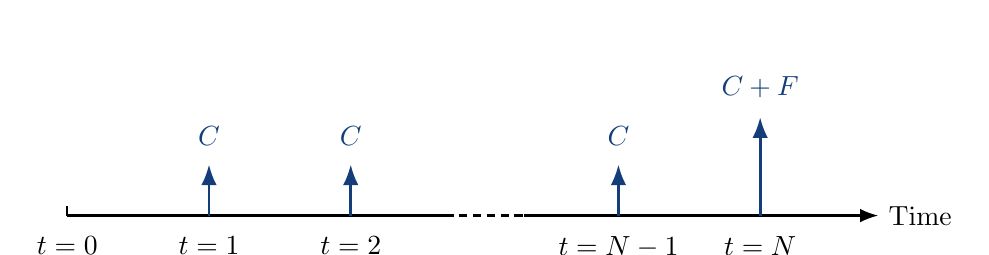
\begin{tikzpicture}[
  >=Latex,
  axis/.style={-Latex, line width=0.8pt},
  cash/.style={-Latex, line width=1.0pt, FinanceBlue},
  tick/.style={line width=0.6pt}
]

% Time axis with a break
\draw[line width=0.8pt] (0,0) -- (4.8,0);

\draw[axis] (5.8,0) -- (10.3,0)
  node[right]{Time};

% Omitted periods
% \node at (5.3,0) {$\cdots$};

% Tick marks
\foreach \x in {0,1.8,3.6,7.0,8.8}
{
  \draw[tick] (\x,0.12) -- (\x,0);
}

% Time labels
\node[below=4pt] at (0,0) {$t=0$};
\node[below=4pt] at (1.8,0) {$t=1$};
\node[below=4pt] at (3.6,0) {$t=2$};
\node[below=4pt] at (7.0,0) {$t=N-1$};
\node[below=4pt] at (8.8,0) {$t=N$};

% Dashed segment indicating omitted coupon periods
\draw[densely dashed, line width=0.8pt]
  (4.8,0) -- (5.8,0);


% Coupon payments
\draw[cash] (1.8,0) -- (1.8,0.65)
  node[above=3pt] {$C$};

\draw[cash] (3.6,0) -- (3.6,0.65)
  node[above=3pt] {$C$};

\draw[cash] (7.0,0) -- (7.0,0.65)
  node[above=3pt] {$C$};

% Final coupon and principal
\draw[cash] (8.8,0) -- (8.8,1.25)
  node[above=3pt] {$C+F$};

\end{tikzpicture}

\caption{Promised Cash Flows of a Conventional Coupon Bond}
\label{fig:ch8-coupon-bond-cashflows}
\end{figure}

The coupon rate determines the contractual coupon payment. It is not the same as the market yield. The coupon rate is fixed by the contract for a conventional fixed-rate bond, whereas the market yield changes with the bond's price and the return investors require.

Bond contracts differ in both coupon and principal-repayment structure. A zero-coupon bond makes no periodic coupon payments, whereas a coupon-bearing bond does. Principal may be repaid under a bullet or an amortizing structure. A bullet bond repays principal at maturity, whereas an amortizing bond repays principal progressively before maturity. If a balance remains outstanding at maturity, the structure is partially amortizing and the final principal payment is called a balloon payment.

These repayment structures distribute the issuer's
cash-payment obligations differently over time.
A bullet structure preserves the full principal
outstanding until maturity but concentrates repayment
at that date. Amortization requires earlier principal
payments, progressively reducing the outstanding
balance and the amount remaining at maturity.

Maturity determines the contractual horizon over which
the debt remains outstanding. A longer maturity extends
the period over which investors are exposed to changes
in the issuer's credit condition. For otherwise similar
fixed-rate bonds, it also generally increases sensitivity
to changes in market interest rates.

\begin{example}{Bullet and Amortizing Structures}{bullet-amortizing-structures}

Consider two three-year bonds with face value RMB~1,000 and an annual coupon rate of 6\%.

A bullet bond pays RMB~60 of interest in each of the first two years and RMB~1,060 at maturity:

\[
60,\qquad 60,\qquad 1,060.
\]

This conventional coupon bond has a bullet principal
structure: no principal is repaid before maturity.
Bullet repayment refers to the timing of principal
repayment rather than the payment of coupons.
A zero-coupon bond that repays its entire face value
at maturity also has a bullet principal structure.

\medskip

Suppose instead that the principal is repaid in three equal annual installments. Interest is calculated on the principal outstanding at the beginning of each year. The payments are then approximately

\[
393.33,\qquad 373.33,\qquad 353.34.
\]

The bullet structure keeps the full principal outstanding until maturity, whereas amortization reduces the principal progressively and lowers subsequent interest payments. 

\end{example}


\subsection{Seniority and Priority of Claims}

Debt claims differ in priority. Seniority specifies the order in which creditors are entitled to receive value when the issuer cannot satisfy all claims in full. Senior claims rank ahead of junior claims, subject to contractual terms and applicable insolvency law. Priority may have little visible effect when all promised payments can be made. In distress, however, it determines how shortfalls are allocated across claims.

Consider an issuer with value $A$ available to senior and subordinated creditors after relevant costs and any claims ranking ahead of them. Suppose the senior claim is $D_S$ and the subordinated claim is $D_J$. In a simplified priority waterfall, the amount recovered by senior creditors $R_S$ is

\begin{equation}
R_S=\min\{D_S,A\},
\label{eq:ch8-senior-recovery}
\end{equation}
while the amount recovered by subordinated creditors is

\begin{equation}
R_J
=
\min\left\{D_J,\max\{A-R_S,0\}\right\}
=
\min\left\{D_J,\max\{A-D_S,0\}\right\}.
\label{eq:ch8-junior-recovery}
\end{equation}

The simplified waterfall abstracts from collateral rights, guarantees, intercreditor agreements, and other legal complexities.

\begin{example}{A Simple Priority Waterfall}{priority-waterfall}

A firm has RMB~100 million of senior debt and RMB~60 million of subordinated debt. If RMB~130 million is available to these creditors, senior creditors recover RMB~100 million and subordinated creditors receive the remaining RMB~30 million, implying a 50\% recovery rate.

If only RMB~80 million is available, senior creditors recover RMB~80 million and subordinated creditors receive nothing.

\end{example}

Priority may also arise from corporate structure. Debt issued by a parent company may be structurally subordinated to debt issued by an operating subsidiary, since subsidiary creditors have claims on subsidiary assets before residual value can be distributed to the parent. Guarantees can reduce this subordination by giving creditors a direct claim against another entity in the group.

Bonds with similar maturities may differ in expected recovery and value when their priority positions differ.

\subsection{Collateral and Creditor Protection}

Collateral gives creditors a security interest in specified assets that may be enforced if the borrower fails to meet its contractual obligations. A secured creditor therefore holds both a payment claim on the borrower and a claim against designated collateral, subject to the validity and enforceability of the security interest.

The protection provided by collateral depends on its realizable value, liquidity, and legal enforceability. If the debt claim is $D$ and the realizable value of pledged collateral is $V_C$, a simple collateral-coverage ratio is

\begin{equation}
CC=\frac{V_C}{D}.
\label{eq:ch8-collateral-coverage}
\end{equation}

A higher coverage ratio may improve expected recovery, but it does not ensure full repayment. Collateral values may decline before default, competing claims may reduce the value available to a creditor, and liquidation or enforcement may be costly.

Collateral can also affect borrower incentives. Assets pledged to creditors are less readily transferred or re-pledged, and their loss in default can reduce the attraction of actions that increase creditor risk. The effectiveness of these protections also depends on the terms of the security agreement and the applicable legal framework.

Different assets provide different degrees of protection. Marketable securities can often be realized more readily than specialized equipment, real estate, or receivables, even when their current appraised values are similar.

Bondholders may also benefit from guarantees. A guarantee gives the creditor a contractual claim against a guarantor rather than a security interest in a specific asset. Collateral and guarantees strengthen creditor protection through different legal mechanisms.

\begin{tcolorbox}[
  enhanced,
  breakable,
  colback=white,
  colframe=FinanceBlue,
  boxrule=0.7pt,
  sharp corners,
  borderline west={2.2pt}{0pt}{FinanceBlue},
  title=\textbf{Financial Perspective: A Secured Bond Is Not risk-free},
  coltitle=white,
  colbacktitle=FinanceBlue,
  fonttitle=\bfseries,
  before skip=1.2em,
  after skip=1.2em
]

A secured bond is not a risk-free bond. Collateral can improve expected recovery if default occurs, but it does not ensure that promised payments will be made. Credit analysis therefore considers both the probability of default and the loss that creditors may bear in default.

\end{tcolorbox}

\subsection{Bond Indentures and Bondholder Rights}

Bond indentures specify the covenants governing the
issuer's financial policies and corporate actions.
Common provisions restrict additional borrowing,
asset disposals, distributions to shareholders, or
changes in corporate control. Others require the
issuer to provide financial information or maintain
specified financial conditions. These provisions
define the contractual protections available to
bondholders.

A covenant breach does not necessarily constitute
an immediate event of default. The consequences depend
on the terms of the indenture, including notice and
cure provisions. If the breach qualifies as an event
of default, bondholders may obtain rights such as
acceleration of repayment or enforcement of security
interests, where applicable. A breach may also lead
to negotiations over waivers or amendments to the
bond contract.

In widely held bond issues, the exercise of these
rights is complicated by dispersed ownership and
collective action problems. A trustee commonly acts
on behalf of bondholders in monitoring compliance,
communicating with the issuer, and administering
contractual remedies. The indenture specifies the
trustee's authority and the voting thresholds required
for collective decisions.

\subsection{Default, Restructuring, and Recovery}

Default occurs when the issuer fails to meet contractual obligations or when a specified event of default occurs under the debt agreement. Failure to pay interest or principal is the clearest case. Other events of default may include specified covenant breaches, cross-defaults, or insolvency events.

Default does not by itself determine the loss on a debt claim. Creditors may recover value through continued payments, collateral realization, restructuring, or liquidation. Let $R$ denote the value recovered and $D$ the contractual claim at default. The recovery rate is

\begin{equation}
RR=\frac{R}{D}.
\label{eq:ch8-recovery-rate}
\end{equation}
Loss given default (LGD) is the proportion of exposure at default that is not recovered:

\begin{equation}
LGD=1-RR.
\label{eq:ch8-lgd}
\end{equation}

Let $PD$ denote the probability of default over the specified horizon, and let $EAD$ denote the exposure outstanding when default occurs. Expected loss over that horizon can be expressed as

\begin{equation}
EL=PD\times LGD\times EAD,
\label{eq:ch8-expected-credit-loss}
\end{equation}
This expression separates the likelihood of default from the loss conditional on default.

Restructuring modifies the original debt contract. It may involve extending maturity, reducing coupon or principal payments, exchanging existing debt for new securities, or converting debt into equity. Restructuring can preserve going-concern value when liquidation would destroy value.

Restructuring outcomes are influenced by priority, collateral, legal rules, and bargaining between the issuer and its creditors and among creditor classes. Dispersed bondholders may also face coordination problems. Voting and amendment provisions can reduce these problems by allowing specified majorities to approve changes that bind affected holders.

Recovery reflects both the value preserved in resolution and the contractual position of the claim. Restructuring or liquidation affects the amount of value available to creditors, while seniority, collateral, guarantees, and legal rules affect how that value is allocated among claims. Debt claims issued by the same firm may have different recovery rates.

\begin{example}{Same Default Probability, Different Expected Loss}{default-and-recovery}

Consider two one-year debt claims, each with an exposure of 100 and a 3\% probability of default. Claim A has an expected recovery rate of 70\% in default, while Claim B has an expected recovery rate of 20\%.

Using this expected-loss measure,

\[
EL_A=0.03\times(1-0.70)\times100=0.9,
\]

whereas

\[
EL_B=0.03\times(1-0.20)\times100=2.4.
\]

The two claims have the same default probability but different expected losses because their expected recoveries differ.

\end{example}

\section{Bond Market Architecture and Price Discovery}

A bond contract defines promised cash flows and creditor rights, but market prices emerge through trading among investors. The organization of issuance, trading, clearing, and settlement affects the costs of finding counterparties, executing transactions, and transferring ownership. These frictions influence market liquidity and the extent to which new information is incorporated into bond prices and yields.

\subsection{Issuers, Investors, and Market Participants}

Bond issuers differ in financing purpose, repayment capacity, and legal structure. Governments issue debt to finance public expenditures and manage public liabilities. Financial institutions and nonfinancial corporations use bonds to obtain term funding, refinance existing obligations, or finance investment. Differences in repayment sources and balance-sheet structure give these claims different credit characteristics.

Investors also differ in liabilities, investment horizons, liquidity needs, and regulatory constraints. Banks may hold bonds for investment, liquidity, or collateral purposes. Insurance companies and pension funds often hold longer-duration assets against long-dated liabilities, while asset managers operate under portfolio mandates and redemption structures that can place greater weight on market liquidity.

These differences create heterogeneous demand across maturities, credit classes, and bond types. Some securities fit the balance-sheet needs or investment constraints of particular investors better than others. The composition of the investor base can therefore influence the range of bonds that issuers are able to place in the market.

Specialized institutions support the connection between issuers and investors. Underwriters and arrangers assist with new issues, rating agencies assess credit quality, dealers support secondary-market transactions, and depositories, custodians, and settlement systems support the holding and transfer of securities. Their principal roles are summarized in Table~\ref{tab:ch8-market-participants}.

\begin{table}[H]
\centering
\caption{Selected Participants and Infrastructure in Bond Markets}
\label{tab:ch8-market-participants}

\begin{tabularx}{\textwidth}{@{}p{3.1cm}Y Y@{}}
\toprule
\textbf{Participant} &
\textbf{Primary role} &
\textbf{Relevant economic concern} \\
\midrule

Governments and public issuers
& Raise public debt financing
& Fiscal capacity, debt sustainability, maturity structure \\

Corporations and financial institutions
& Raise debt capital
& Funding needs, leverage, refinancing, credit quality \\

Banks, insurers, pension funds, and asset managers
& Invest in and trade bonds
& Return, duration, liquidity, credit exposure, regulation \\

Underwriters and arrangers
& Structure, underwrite, and distribute bond issues
& Due diligence, pricing, investor demand, distribution risk \\

Credit rating agencies
& Assess issuer and issue credit risk
& Rating quality, methodology, information, conflicts of interest \\

Dealers
& Make markets and support secondary-market trading
& Trading capacity, inventory risk, funding, market liquidity \\

Bond trustees
& Represent bondholders and administer contractual rights
& Covenant compliance, collective action, enforcement \\

Depositories, custodians, and settlement systems
& Maintain securities records, safeguard assets, and facilitate settlement
& Safekeeping, record accuracy, settlement finality, operational risk \\

\bottomrule
\end{tabularx}
\end{table}

\subsection{Primary and Secondary Bond Markets}

The primary market is where new bonds are issued and funds are raised from investors. The secondary market is where outstanding bonds are traded after issuance. The distinction separates the financing transaction from the subsequent transfer of the claim.

Government bonds are often issued through auctions, while corporate and financial bonds commonly use underwriters, syndicates, or bookbuilding processes. Issuance mechanisms differ across jurisdictions and instruments, but they address a common problem: matching the amount, maturity, contractual terms, and pricing of a new issue with investor demand.

Primary-market issuance also aggregates information. Auctions, order books, and investor indications reveal demand at different yields or prices. This information helps determine the terms at which the issue can be placed and how the bonds are allocated among investors. The issue price provides an initial market valuation of the new claim.

Once issued, a bond can be transferred among investors in the secondary market without changing the issuer's contractual obligation. This separates the issuer's financing horizon from the holding period of an individual investor. A ten-year bond can provide ten-year funding even when particular investors hold it for much shorter periods.

\begin{figure}[H]
\centering

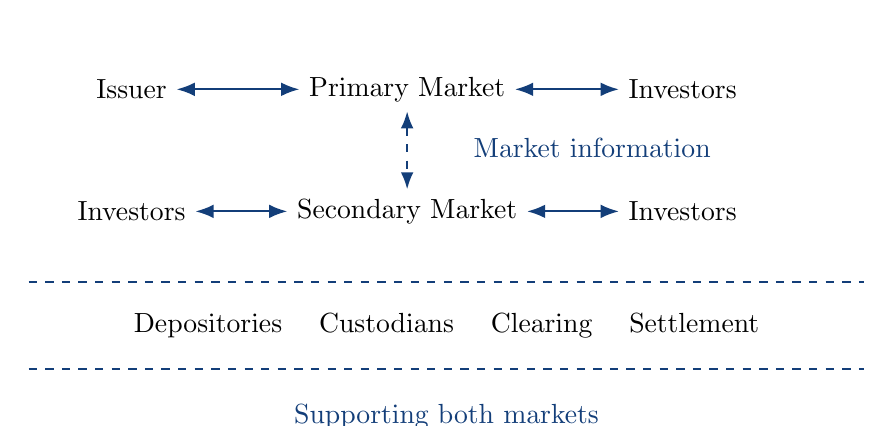
\begin{tikzpicture}[
  >=Latex,
  node/.style={
    align=center,
    font=\normalsize
  },
  flow/.style={
    Latex-Latex,
    line width=0.8pt,
    draw=FinanceBlue
  },
  info/.style={
    Latex-Latex,
    dashed,
    line width=0.7pt,
    draw=FinanceBlue
  },
  infra/.style={
    draw=FinanceBlue,
    line width=0.7pt,
    rounded corners=2pt,
    align=center,
    minimum width=10.6cm,
    minimum height=1.0cm,
    inner sep=6pt
  }
]

% Primary market
\node[node] (issuer) at (0,2.0) {Issuer};
\node[node] (primary) at (3.5,2.0) {Primary Market};
\node[node] (investors1) at (7.0,2.0) {Investors};

\draw[flow] (issuer) -- (primary);
\draw[flow] (primary) -- (investors1);

% Market information
\node[node, text=FinanceBlue] (info) at (5.85,1.25)
{Market information};

% Secondary market
\node[node] (investors2) at (0,0.45) {Investors};
\node[node] (secondary) at (3.5,0.45) {Secondary Market};
\node[node] (investors3) at (7.0,0.45) {Investors};

\draw[flow] (investors2) -- (secondary);
\draw[flow] (secondary) -- (investors3);

\draw[info] (primary.south) --  (secondary.north);

% Infrastructure
\node[
  align=center,
  minimum width=10.6cm,
  minimum height=1.0cm,
  inner sep=6pt
] (infra) at (4.0,-1.)
{Depositories \quad Custodians \quad Clearing \quad Settlement};

\draw[
  dashed,
  draw=FinanceBlue,
  line width=0.7pt
]
([yshift=0.55cm]infra.west) -- ([yshift=0.55cm]infra.east);

\draw[
  dashed,
  draw=FinanceBlue,
  line width=0.7pt
]
([yshift=-0.55cm]infra.west) -- ([yshift=-0.55cm]infra.east);

\node[
  align=center,
  text=FinanceBlue
] at (4.0,-2.15)
{Supporting both markets};

\end{tikzpicture}

\caption{Primary and secondary bond markets}
\label{fig:ch8-primary-secondary-markets}
\end{figure}

Secondary-market trading generates observable prices
and yields for outstanding bonds. These prices
incorporate changing information about interest
rates, credit conditions, and investor demand.
They provide valuation references for existing bonds
and help determine the pricing and terms of subsequent
issuance. An increase in secondary-market yields,
for example, may raise the financing costs faced by
issuers returning to the market.

\subsection{Dealers, Trading, and Market Liquidity}

Many bond markets rely substantially on dealer intermediation. Investors may request quotations from dealers rather than submit every order to a centralized order book. A dealer can buy from one investor and later sell to another, holding the bond in inventory between the two transactions.

A dealer's bid is the price at which the dealer is willing to buy, while the ask is the price at which the dealer is willing to sell. The bid--ask spread reflects transaction costs, inventory risk, adverse selection, and the use of funding and balance-sheet capacity.

Market liquidity has several dimensions. Tightness refers to the cost of executing a trade and is often reflected in bid--ask spreads. Depth refers to the amount that can be traded without a substantial price change. Resiliency refers to the speed with which prices and trading conditions recover after a large trade or market disturbance.

Liquidity varies across bonds. Recently issued benchmark government bonds may trade frequently and in large amounts, while older issues or small corporate bonds may trade only occasionally. Bonds issued by the same borrower can therefore differ substantially in liquidity.

Dealer balance sheets influence the provision of liquidity. A dealer that acquires a bond before finding another buyer must finance the position and bear the risk of an adverse price movement. Higher funding costs, greater price volatility, or tighter balance-sheet constraints may reduce the inventory a dealer is willing to hold and make intermediation more costly.

Electronic trading changes the organization of this process. Request-for-quote systems can facilitate competition among dealers, while other platforms automate parts of quotation and execution. Post-trade transparency provides information about recent transactions, although greater transparency may also affect the willingness of dealers to intermediate large or difficult trades.

\begin{figure}[H]
\centering

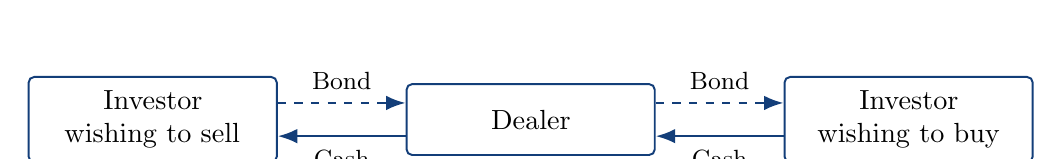
\begin{tikzpicture}[
  >=Latex,
  box/.style={
    draw=FinanceBlue,
    line width=0.7pt,
    rounded corners=2pt,
    align=center,
    text width=2.8cm,
    minimum height=0.9cm,
    inner sep=5pt
  },
  cash/.style={
    -Latex,
    line width=0.9pt,
    draw=FinanceBlue
  },
  bond/.style={
    -Latex,
    dashed,
    line width=0.9pt,
    draw=FinanceBlue
  },
  label/.style={
    font=\small,
    fill=white,
    inner sep=1.5pt
  }
]

% Participants
\node[box] (seller) at (-4.8,0)
  {Investor\\wishing to sell};

\node[box] (dealer) at (0,0)
  {Dealer};

\node[box] (buyer) at (4.8,0)
  {Investor\\wishing to buy};

% Seller to dealer: bond transfer
\draw[bond]
  ([yshift=6pt]seller.east) --
  node[label, above=3pt] {Bond}
  ([yshift=6pt]dealer.west);

% Dealer to seller: cash payment
\draw[cash]
  ([yshift=-6pt]dealer.west) --
  node[label, below=3pt] {Cash}
  ([yshift=-6pt]seller.east);

% Dealer to buyer: bond transfer
\draw[bond]
  ([yshift=6pt]dealer.east) --
  node[label, above=3pt] {Bond}
  ([yshift=6pt]buyer.west);

% Buyer to dealer: cash payment
\draw[cash]
  ([yshift=-6pt]buyer.west) --
  node[label, below=3pt] {Cash}
  ([yshift=-6pt]dealer.east);

\end{tikzpicture}

\caption{Dealer Intermediation in Secondary Bond Trading}
\label{fig:ch8-dealer-intermediation}
\end{figure}

By acting as a principal, the dealer temporarily
holds the bond inventory and bears the associated
inventory and funding risks. The difference between
the buying and selling prices contributes to the
dealer's trading revenue.

\begin{tcolorbox}[
  enhanced,
  breakable,
  colback=white,
  colframe=FinanceBlue,
  boxrule=0.7pt,
  sharp corners,
  borderline west={2.2pt}{0pt}{FinanceBlue},
  title=\textbf{Financial Perspective: Low Credit Risk Does Not Imply High Liquidity},
  coltitle=white,
  colbacktitle=FinanceBlue,
  fonttitle=\bfseries,
  before skip=1.2em,
  after skip=1.2em
]

A bond can have low default risk and still be difficult or costly to trade. Credit risk concerns losses associated with failure to meet contractual payments, while market liquidity concerns the ability to trade the claim without substantial cost or price impact. The two can interact under stress but remain distinct dimensions of risk.

\end{tcolorbox}

\section{Valuation and Risk of Debt Contracts}

Bond valuation links contractual cash flows to market discount rates. For an option-free bond without default risk, value is the present value of promised coupons and principal. Changes in benchmark interest rates affect the discounting of these cash flows, while credit risk affects expected payments and the spread investors require.

\subsection{Bond Prices, Yields, and Contractual Cash Flows}

Consider a bond with promised cash flow $CF_t$ at the end of term $t$, for $t=1,\ldots,T$. If a continuously compounded yield $y$ is used to discount all promised cash flows, the bond price is

\begin{equation}
P(y)
=
\sum_{t=1}^{T}
CF_t e^{-yt}.
\label{eq:ch8-bond-price}
\end{equation}

For a plain-vanilla bond, $CF_t=C$ for $t=1,\ldots,T-1$, and $CF_T=C+F$.

The yield to maturity (YTM) is the single discount
rate that equates the present value of a bond's
promised cash flows to its observed market price.
It does not necessarily equal the investor's realized
return. The realized return depends on whether
promised payments are made, the rates at which
interim coupons are reinvested, and, if the bond
is sold before maturity, the price received at sale.

For a default-free bond, each cash flow can instead be discounted at the spot rate corresponding to its maturity. Let $s_t$ denote the continuously compounded spot rate for a cash flow received at date $t$. Then

\begin{equation}
P
=
\sum_{t=1}^{T}
CF_t e^{-s_t t}.
\label{eq:ch8-bond-price-spot-rates}
\end{equation}

For a plain-vanilla bond with fixed positive cash flows, price is a decreasing function of yield. Differentiating Equation~\ref{eq:ch8-bond-price} with respect to $y$ gives

\begin{equation}
\frac{dP}{dy}
=
-\sum_{t=1}^{T}
tCF_t e^{-yt}
<0.
\label{eq:ch8-price-yield-negative}
\end{equation}

This inverse relation also determines whether a conventional fixed-rate bond trades at par, at a premium, or at a discount. When coupon and yield are expressed on the same periodic basis, the bond is priced at par if the coupon rate equals the yield to maturity, above par if the coupon rate exceeds the yield, and below par if the coupon rate is lower than the yield.

\begin{example}{A Coupon Bond Priced from Its Yield}{coupon-bond-price-yield}

A five-year bond has face value 100 and pays a 5\% annual coupon. At a continuously compounded yield of 4\%, its price is

\[
P
=
5e^{-0.04\times1}
+
5e^{-0.04\times2}
+
5e^{-0.04\times3}
+
5e^{-0.04\times4}
+
105e^{-0.04\times5}
=
104.08.
\]

The bond trades above par. Let $y_{\mathrm{par}}$ denote the continuously compounded yield that prices the bond at its face value. It satisfies

\[
100
=
5e^{-y_{\mathrm{par}}}
+
5e^{-2y_{\mathrm{par}}}
+
5e^{-3y_{\mathrm{par}}}
+
5e^{-4y_{\mathrm{par}}}
+
105e^{-5y_{\mathrm{par}}}.
\]

For this bond,

\[
y_{\mathrm{par}}
=
\ln(1.05)
\approx
4.879\%.
\]

The assumed continuously compounded yield of 4\%
is below this par yield, which is consistent with
a price above 100. A yield above $y_{\mathrm{par}}$
would imply a price below par.

\end{example}

Figure~\ref{fig:ch8-price-yield-curve} illustrates
the inverse relationship between bond prices and
yields, including the two values calculated above.


\begin{figure}[H]
\centering

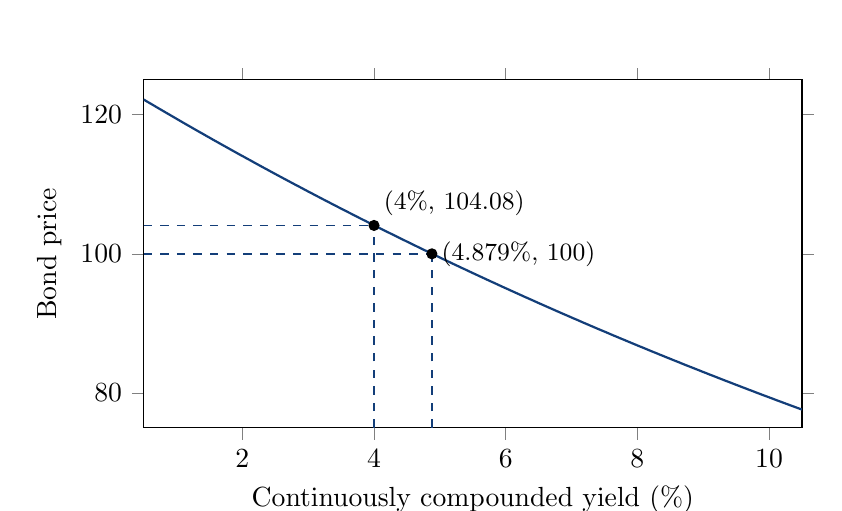
\begin{tikzpicture}
\begin{axis}[
  width=0.82\textwidth,
  height=6.0cm,
  xmin=0.5,
  xmax=10.5,
  ymin=75,
  ymax=125,
  xlabel={Continuously compounded yield (\%)},
  ylabel={Bond price},
  axis lines=box,
  grid=none,
  tick align=outside
]

\addplot[
  FinanceBlue,
  thick,
  domain=0.5:10.5,
  samples=200
]
{
  5*exp(-x/100)
  +5*exp(-2*x/100)
  +5*exp(-3*x/100)
  +5*exp(-4*x/100)
  +105*exp(-5*x/100)
};

\addplot[
  only marks,
  mark=*,
  mark size=1.8pt
]
coordinates {(4,104.08) (4.879,100)};

% dashed guide lines for (4, 104.08)
\addplot[
  dashed,
  FinanceBlue,
  line width=0.6pt
]
coordinates {(4,75) (4,104.08)};

\addplot[
  dashed,
  FinanceBlue,
  line width=0.6pt
]
coordinates {(0.5,104.08) (4,104.08)};

% dashed guide lines for (4.879, 100)
\addplot[
  dashed,
  FinanceBlue,
  line width=0.6pt
]
coordinates {(4.879,75) (4.879,100)};

\addplot[
  dashed,
  FinanceBlue,
  line width=0.6pt
]
coordinates {(0.5,100) (4.879,100)};

\node[
  anchor=south west,
  font=\small
] at (axis cs:4,104.08)
{$(4\%,\,104.08)$};

\node[
  anchor=west,
  font=\small
] at (axis cs:4.879,100)
{$(4.879\%,\,100)$};

\end{axis}
\end{tikzpicture}

\caption{Price--yield relation for a five-year 5\% coupon bond under continuous compounding}
\label{fig:ch8-price-yield-curve}
\end{figure}

\subsection{Interest Rate Risk, Duration, and Convexity}

Interest rate risk is the risk that changes in market yields alter the value of a fixed-income claim. For a bond with fixed contractual cash flows, a rise in yield reduces present value, while a decline in yield increases it. The magnitude of the price response depends on the timing of the bond's cash flows: sensitivity is generally greater when a larger share of present value is associated with later payments.

Duration provides a first-order measure of this sensitivity. It summarizes the timing of a bond's present-valued cash flows. For a bond priced at yield $y$ with cash flow $CF_t$ at date $t$, duration is

\begin{equation}
D=\frac{1}{P(y)}
\sum_{t=1}^{T}
t\,CF_t e^{-yt}.
\label{eq:ch8-macaulay-duration}
\end{equation}

The weights $w_t = CF_t e^{-yt}/P(y)$ represent the share of the bond's present value attributable to each cash flow. Duration is thus the present-value-weighted average time to receipt of the bond's cash flows.

For a zero-coupon bond,  duration equals maturity, since the entire cash flow is received at maturity. For a coupon bond, earlier coupon payments place part of the present-value weight before maturity, making duration shorter than maturity. Holding maturity and yield constant, a higher coupon generally reduces duration.

Duration measures the first-order sensitivity of bond price to changes in the continuously compounded yield. Differentiating Equation~(\ref{eq:ch8-bond-price}) with respect to $y$ gives

\begin{equation}
\frac{dP(y)}{dy}=-\sum_{t=1}^{T}
tCF_t e^{-yt}.
\label{eq:ch8-price-yield-derivative}
\end{equation}

\begin{equation}
D=
\frac{1}{P(y)}
\sum_{t=1}^{T}
tCF_t e^{-yt}
=
-\frac{1}{P(y)}
\frac{dP(y)}{dy}
.
\label{eq:ch8-duration}
\end{equation}

Then, 

\begin{equation}
\frac{\Delta P(y)}{P(y)}
\approx
-D \Delta y.
\label{eq:ch8-duration-price-change}
\end{equation}

\begin{example}{Using Duration to Approximate a Bond Price Change}{duration-price-approximation}

Consider again the five-year 5\% coupon bond in Example~\ref{ex:coupon-bond-price-yield}. At a continuously compounded yield of 4\%, its price is approximately 104.08 and its duration is 4.556.

Suppose the yield rises by 50 basis points, so that

\[
\Delta y=0.005.
\]

Using duration,

\[
\frac{\Delta P}{P}
\approx
-D\Delta y
=
-4.556(0.005)
=
-2.278\%.
\]

The approximate new bond price is

\[
P_{\mathrm{new}}
\approx
104.08\times(1-0.02278)
=
101.71.
\]

Direct repricing at a continuously compounded yield of 4.5\% gives

\[
P
=
5e^{-0.045\times1}
+
5e^{-0.045\times2}
+
5e^{-0.045\times3}
+
5e^{-0.045\times4}
+
105e^{-0.045\times5}
=
101.74.
\]

The duration-based estimate is 101.71, compared with
the exact repriced value of 101.74.

\end{example}

Bond yields may also be quoted with compounding more than once a year. Suppose $y$ is a nominal annual yield compounded $n$ times per year. For cash flows received at times $t$ measured in years, the bond price is

\begin{equation}
P(y)
=
\sum_{t}
\frac{CF_t}{(1+y/n)^{nt}}.
\label{eq:ch8-bond-price-n-compounding}
\end{equation}

The corresponding modified duration is 
\begin{equation}
D_{\mathrm{mod}}
=
\frac{D}{1+y/n}.
\label{eq:ch8-modified-duration-relation}
\end{equation}

Modified duration is thus the price sensitivity associated with a discretely compounded yield convention. Under continuous compounding, the duration defined earlier directly measures this sensitivity.

Duration provides a local linear approximation to the price--yield relation. As the change in yield becomes larger, the curvature of this relation becomes more important and the duration approximation becomes less accurate. Convexity captures this second-order sensitivity. Under continuous compounding,

\begin{equation}
\mathrm{C}
=
\frac{1}{P(y)}
\frac{d^2P(y)}{dy^2}
=
\frac{1}{P(y)}
\sum_{t=1}^{T}
t^2 CF_t e^{-yt}.
\label{eq:ch8-convexity}
\end{equation}

Including convexity gives the second-order approximation

\begin{equation}
\frac{\Delta P}{P}
\approx
-D\,\Delta y
+
\frac{1}{2}\mathrm{C}(\Delta y)^2.
\label{eq:ch8-duration-convexity-approx}
\end{equation}

The convexity term improves the duration approximation as the change in yield increases.

For a plain-vanilla bond with fixed positive cash flows, convexity is positive. A decline in yield produces a larger price increase than the duration-only approximation predicts, while an equal increase in yield produces a smaller price decline.

\begin{example}{Duration and Convexity as Risk Measures}{duration-convexity-risk}

Consider the five-year 5\% coupon bond in Example~\ref{ex:coupon-bond-price-yield}, priced at a continuously compounded yield of 4\%. Its price is approximately 104.08 and its duration is 4.556. 

For a 50-basis-point increase in yield, the duration approximation gives

\[
\frac{\Delta P}{P}
\approx
-D\Delta y
=
-4.556\times 0.005
=
-2.278\%.
\]

The bond's convexity is approximately 21.911.

Including the second-order term gives

\[
\frac{\Delta P}{P}
\approx
-2.278\%
+\frac{1}{2}\times 21.911\times (0.005)^2
=
-2.251\%.
\]

\[
P_{\mathrm{new}}
\approx
104.08\times(1-0.02251)
=
101.73.
\]

Direct repricing at a continuously compounded yield
of 4.5\% gives a price of approximately 101.74.
The convexity-adjusted estimate is closer to this
value than the duration-only estimate.

\end{example}

\begin{figure}[H]
\centering

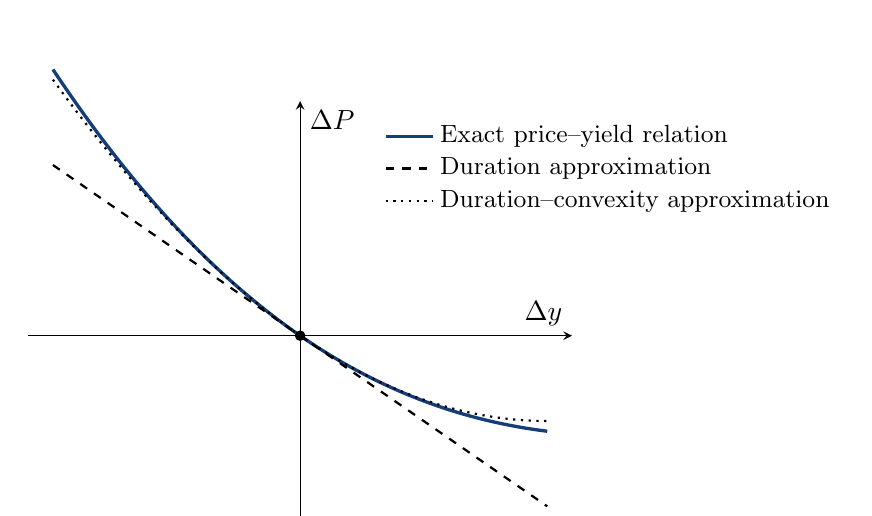
\begin{tikzpicture}
\begin{axis}[
  width=0.7\textwidth,
  height=7.0cm,
  xmin=-2.2,
  xmax=2.2,
  ymin=-18,
  ymax=22,
  axis lines=middle,
  xlabel={$\Delta y$},
  ylabel={$\Delta P$},
  xtick=\empty,
  ytick=\empty,
  tick align=outside,
  enlargelimits=false,
  clip=false,
 legend style={
  at={(1.5,0.97)},
  anchor=north east,
  draw=none,
  fill=none,
  font=\small
},
  legend cell align=left
]

% Exact price-yield relation
\addplot[
  FinanceBlue,
  very thick,
  domain=-2:2,
  samples=200
]
{-8*x + 2*x^2 - 0.12*x^3};
\addlegendentry{Exact price--yield relation}

% Duration approximation
\addplot[
  black,
  dashed,
  thick,
  domain=-2:2,
  samples=2
]
{-8*x};
\addlegendentry{Duration approximation}

% Duration-convexity approximation
\addplot[
  black,
  dotted,
  thick,
  domain=-2:2,
  samples=200
]
{-8*x + 2*x^2};
\addlegendentry{Duration--convexity approximation}

% Origin
\addplot[
  only marks,
  mark=*,
  mark size=1.7pt
]
coordinates {(0,0)};

\end{axis}
\end{tikzpicture}

\caption{A schematic illustration of duration and convexity in approximating bond price changes}
\label{fig:ch8-duration-convexity-concept}
\end{figure}

Figure~\ref{fig:ch8-duration-convexity-concept} illustrates the local linear approximation provided by duration and the curvature adjustment captured by convexity.

Duration also has an economic interpretation. A longer-duration bond places a larger share of its present value in later cash flows and is more sensitive to changes in discount rates. This is consistent with the general valuation principle that more distant cash flows are more sensitive to the rate at which they are discounted.

Duration and convexity do not capture all dimensions of bond risk. Credit spreads may change independently of benchmark rates, yield-curve movements need not be parallel, and embedded options can alter cash flows as interest rates change. In practice, these measures are often supplemented by additional measures of curve, spread, and option risk.

\subsection{Credit Spreads in Bond Pricing}

A credit-risky bond often trades at a yield above a benchmark bond or curve of comparable maturity. When the two yields are measured on the same basis, their difference is the yield spread:

\begin{equation}
spread
=
y_{\mathrm{credit}}
-
y_{\mathrm{benchmark}}.
\label{eq:ch8-credit-spread}
\end{equation}

An observed spread can reflect expected default losses, compensation for bearing losses in adverse states, market liquidity, uncertainty, tax treatment, embedded options, and other instrument-specific features. It should not be interpreted directly as a default probability.

A spread can also be incorporated into valuation by adding it to the benchmark spot-rate curve. Let $r_t$ denote the continuously compounded benchmark spot rate for maturity $t$, and let $z$ denote a constant spread added to each maturity. The bond price is then

\begin{equation}
P(z)
=
\sum_{t=1}^{T}
CF_t e^{-(r_t+z)t}.
\label{eq:ch8-spread-price}
\end{equation}

The constant $z$ that equates the present value of the promised cash flows to the observed bond price is commonly called the Z-spread. It summarizes the additional yield required over the benchmark spot curve under the assumption of a constant spread across maturities. Bonds with embedded options or more complex contingent cash flows require additional treatment.

Credit-spread movements can change bond prices even when benchmark interest rates remain unchanged. Suppose a corporate bond yield rises from 5.0 to 6.0\% entirely as a result of a one-percentage-point increase in its spread. With the benchmark curve unchanged, the higher spread reduces the present value of the bond's promised cash flows.

A bond's yield can also rise when benchmark rates increase while its credit spread remains unchanged. The resulting price decline may appear similar, but its economic source is different. Separating benchmark-rate movements from spread movements is therefore important in analyzing bond returns and risk.

Contractual features also affect credit spreads. Seniority, collateral, and guarantees can improve expected recovery, while covenants can limit actions that weaken creditor protection. Maturity changes the horizon over which credit risk is borne. Bonds issued by the same firm can therefore trade at different spreads when their contractual positions differ.

Liquidity can contribute to these differences. A bond that trades infrequently or requires a substantial price concession for immediate sale may carry a wider spread than a more liquid bond with similar credit characteristics. During periods of market stress, credit and liquidity effects may move together and become difficult to separate.

\begin{example}{Separating Benchmark and Spread Movements}{benchmark-spread-decomposition}

A five-year corporate bond initially yields 5.2\%, while the five-year benchmark yield is 3.4\%, with both yields measured on the same basis. The bond's spread is

\[
5.2\%-3.4\%=1.8\%,
\]

or 180 basis points.

One month later, the corporate yield is 6.1\% and the benchmark yield is 3.6\%. The new spread is 250 basis points. The corporate yield has risen by 90 basis points, of which 20 basis points reflect the increase in the benchmark yield and 70 basis points reflect spread widening.

The change in the corporate yield therefore contains two economically distinct components: a movement in the benchmark rate and a movement in the credit spread.

\end{example}

%========================================================
% Summary
%========================================================

\TailModule{summary}{Summary}

A bond is a debt contract that specifies promised cash flows, maturity, priority, and other creditor rights. Coupon and principal-repayment structures determine the timing of promised payments, while seniority and collateral influence how losses are allocated in distress. Covenants restrict or require specified actions, and default provisions determine when creditors can exercise additional rights. Recovery depends on contractual priority, collateral, guarantees, restructuring, and the legal and institutional environment.

Bond markets connect issuers with investors through both primary and secondary markets. Primary issuance determines the terms on which new debt is sold, while secondary trading allows investors to transfer existing claims without changing the issuer's contractual obligations. Dealers support trading and liquidity by standing between buyers and sellers, while trading platforms facilitate quotation and execution. Dealer intermediation is influenced by inventory risk, funding conditions, information, and balance-sheet capacity.

Bond valuation begins with contractual cash flows. Yield to maturity is the single discount rate that equates the present value of promised cash flows with the observed price, while spot-rate valuation applies maturity-specific discount rates. For bonds with fixed positive cash flows, price and yield move in opposite directions. Duration provides a first-order measure of price sensitivity to yield changes, while convexity captures the curvature of the price--yield relation and improves the approximation for larger changes.

Credit spreads measure the additional yield on a credit-risky bond relative to a benchmark, but they are not pure measures of default probability. Expected default losses, compensation for bearing losses in adverse states, liquidity, contractual features, and market conditions can all contribute to the spread. Bond prices thus reflect both the rights embedded in the debt contract and the market's changing valuation of those rights.

%========================================================
% Key Terms
%========================================================

\TailModule{keyterms}{Key Terms}

Bond; face value; coupon rate; coupon payment; maturity; bullet bond; amortizing bond; zero-coupon bond; seniority; subordinated debt; collateral; guarantee; covenant; control right; default; restructuring; recovery rate; loss given default; primary bond market; secondary bond market; dealer; bid--ask spread; market liquidity; yield to maturity; spot-rate valuation; premium bond; discount bond; duration; modified duration; convexity; benchmark yield; credit spread; Z-spread; liquidity premium.

%========================================================
% Financial AI Lab
%========================================================

\TailModule{aiprompt}{Financial AI Lab}

\textbf{Lab: Audit a Bond Valuation and Risk Report}

Choose an actively traded, option-free government or corporate bond for which the face value, coupon rate, coupon frequency, maturity date, and market price can be verified from authoritative sources. Ask an AI system to calculate the bond's yield to maturity, duration, and convexity, stating the yield and compounding conventions used.

Audit the report in four stages.

\begin{enumerate}

\item \textbf{Verify the contract.}

Check the coupon rate, payment frequency, maturity, face value, and whether the bond contains any embedded option. Confirm whether the quoted market price is clean or dirty and identify the convention used to calculate accrued interest.

\item \textbf{Reproduce the valuation.}

Construct the contractual cash flows independently and verify that discounting them at the reported yield reproduces the settlement price on a consistent basis. Check cash-flow timing, compounding convention, units, coupon frequency, and the treatment of accrued interest.

\item \textbf{Stress the yield.}

Increase and decrease the yield by 50 basis points. Calculate the exact repriced bond values and compare them first with the duration approximation and then with the duration--convexity approximation. Explain the direction and magnitude of the approximation errors.

\item \textbf{Separate benchmark and spread risk.}

If a credit-risky bond is selected, compare its yield with an appropriate benchmark of similar maturity. Ask the AI system to explain the observed spread. Identify which parts of the explanation are directly supported by data and which require additional evidence about default risk, expected recovery, liquidity, contractual features, or market conditions.

\end{enumerate}

The final report should identify at least one case in which a numerically correct calculation could still lead to a financially misleading conclusion.

%========================================================
% Discussion Questions
%========================================================

\TailModule{questions}{Discussion Questions}

\begin{enumerate}

\item Why can two bonds issued by the same firm and maturing on the same date have different yields? Explain using priority, collateral, covenants, and liquidity.

\item Why is yield to maturity not necessarily the return an investor will actually realize on a bond?

\item Why does duration provide only a local approximation to a bond's price response to changes in yield? How does convexity improve this approximation?

\item A bond's yield rises by 80 basis points while the benchmark yield rises by only 20 basis points. What additional information is needed before attributing the remaining change to default risk?

\end{enumerate}

%========================================================
% Applied Problems
%========================================================

\TailModule{appprobs}{Applied Problems}

\begin{enumerate}

\item \textbf{Contractual cash flows.}

A bond has face value RMB~1,000, a 6\% annual coupon rate, semiannual coupon payments, and four years to maturity.

\begin{enumerate}

\item Calculate each semiannual coupon payment.

\item How many coupon payments remain?

\item State the final contractual payment at maturity.

\item Explain which of these contractual cash flows changes if market yields rise immediately after the bond is issued.

\end{enumerate}

\item \textbf{Priority and recovery.}

A distressed firm has RMB~150 million available for two classes of debt. Senior debt has a contractual claim of RMB~120 million and subordinated debt has a claim of RMB~80 million.

\begin{enumerate}

\item Calculate the amount recovered by each class under strict priority.

\item Calculate the recovery rate for each class.

\item Recalculate the recoveries if the value available to creditors falls to RMB~90 million.

\item Explain why the two classes can have different credit spreads before default even though they are obligations of the same issuer.

\end{enumerate}

\item \textbf{Bond price and yield.}

A five-year bond has face value 100 and pays a 4\% annual coupon.

\begin{enumerate}

\item Calculate its price if the continuously compounded yield to maturity is 3\%.

\item Recalculate the price at a continuously compounded yield of 5\%.

\item Identify whether the bond trades at a premium or discount in each case.

\item Verify that the direction of the price change is consistent with the price--yield relation.

\end{enumerate}

\item \textbf{Spot-rate valuation.}

A three-year bond has face value 100 and pays a 5\% annual coupon. The continuously compounded one-, two-, and three-year spot rates are 3.0, 3.6, and 4.1\%.

\begin{enumerate}

\item Price the bond using the spot-rate curve.

\item Explain why discounting every cash flow at the three-year spot rate would not be equivalent.

\item Find the continuously compounded yield to maturity that approximately reproduces your price.

\item Explain the economic difference between the spot rates and the yield to maturity.

\end{enumerate}

\item \textbf{Duration and convexity.}

A bond has duration of 6.2 and convexity of 48. Its current price is 102. Assume yields are continuously compounded.

\begin{enumerate}

\item Estimate the percentage price change for a 40-basis-point increase in yield using duration only.

\item Add the convexity adjustment.

\item Estimate the new price using the duration--convexity approximation.

\item Explain why the convexity term has the same sign for equal increases and decreases in yield.

\end{enumerate}

\item \textbf{Benchmark rates and credit spreads.}

A seven-year corporate bond yields 5.8\% when a comparable benchmark bond yields 3.7\%, with both yields measured on the same basis.

\begin{enumerate}

\item Calculate the initial spread in basis points.

\item One month later, the corporate yield is 6.4\% and the benchmark yield is 3.9\%. Calculate the new spread.

\item Decompose the 60-basis-point increase in the corporate yield into the benchmark-rate change and the spread change.

\item Give three possible reasons for the spread change and explain what evidence would be needed to distinguish among them.

\end{enumerate}

\end{enumerate}

%========================================================
% Data Application
%========================================================

\TailModule{dataapp}{Data Application}

\textbf{Government Curves, Credit Curves, and Bond-Market Pricing in China}

Use ChinaBond yield-curve data published by China Central Depository \& Clearing Co., Ltd. Select a government bond yield curve and at least one credit-related curve, such as a high-grade corporate or commercial-bank bond curve. Use common maturities and, as far as possible, the same yield definition and observation basis.

First, plot the selected curves for a common observation date and calculate the spread between the credit curve and the government curve at each common maturity. Examine whether the spread is approximately constant across maturities or varies along the curve.

Second, repeat the analysis for an earlier observation date. For each maturity, decompose the change in the credit yield into the change in the government yield and the change in the spread:

\[
\Delta y_{\mathrm{credit},t}
=
\Delta y_{\mathrm{government},t}
+
\Delta s_t.
\]

Identify the maturities at which the credit spread changed most and compare these changes with movements in the government curve.

Third, interpret the results cautiously. A wider spread between a credit curve and the government curve can reflect expected credit losses, risk premia, market liquidity, investor demand, issuer characteristics, or differences in curve construction. A change in the observed spread should not be interpreted directly as a change in default probability.

Report the observation dates, curve names, maturities, yield definitions, and data source. If the source provides different types of curves, such as yield-to-maturity and spot-rate curves, state which one is used and explain the choice. Where possible, examine whether the underlying securities differ in liquidity, issuer type, credit quality, or contractual structure before interpreting the spread economically.

%========================================================
% Further Reading
%========================================================

\TailModule{furtherread}{Further Reading}

\begin{itemize}

\item Macaulay, Frederick R. (1938),
\emph{Some Theoretical Problems Suggested by the Movements of Interest Rates, Bond Yields and Stock Prices in the United States since 1856},
National Bureau of Economic Research.

\item Fisher, Lawrence, and Roman L. Weil (1971),
``Coping with the Risk of Interest-Rate Fluctuations: Returns to Bondholders from Na\"ive and Optimal Strategies,''
\emph{The Journal of Business}, 44(4), 408--431.

\item Merton, Robert C. (1974),
``On the Pricing of Corporate Debt: The Risk Structure of Interest Rates,''
\emph{The Journal of Finance}, 29(2), 449--470.

\item Duffie, Darrell, and Kenneth J. Singleton (1999),
``Modeling Term Structures of Defaultable Bonds,''
\emph{The Review of Financial Studies}, 12(4), 687--720.

\item Bessembinder, Hendrik, William Maxwell, and Kumar Venkataraman (2006),
``Market Transparency, Liquidity Externalities, and Institutional Trading Costs in Corporate Bonds,''
\emph{Journal of Financial Economics}, 82(2), 251--288.

\end{itemize}

\ChapterTail{summary,keyterms,aiprompt,questions,appprobs,dataapp,furtherread}

\chapter{Stock Markets and Equity Claims}
\label{chap:Stock_Markets_and_Equity_Claims}

\begin{openingcase}{Why Can Market Value Change When No Cash Changes Hands?}

A listed company has 100 million shares outstanding, and its shares trade at RMB~10. The company's market value of equity is RMB~1 billion. One morning, the company announces that a new product has passed an important technical milestone. No dividend is paid, no new shares are issued, and no cash enters the company. Yet investors revise their expectations about future profits, and the share price rises to RMB~12.

The company's market value of equity has increased by RMB~200 million even though the company did not receive RMB~200 million of new financing. The change occurred in the secondary market, where investors exchanged existing shares with one another.

\end{openingcase}

\begin{tcolorbox}[
  enhanced,
  colback=FinanceBlue!6,
  colframe=FinanceBlue,
  boxrule=0.6pt,
  sharp corners,
  left=8pt,
  right=8pt,
  top=7pt,
  bottom=7pt,
  before skip=1em,
  after skip=1.6em,
  title=\textbf{Core Questions},
  coltitle=white,
  colbacktitle=FinanceBlue,
  fonttitle=\bfseries,
  attach boxed title to top left={xshift=6pt,yshift=-2mm},
  boxed title style={
    boxrule=0pt,
    sharp corners,
    left=5pt,
    right=5pt,
    top=2pt,
    bottom=2pt
  }
]
\begin{enumerate}[
  leftmargin=*,
  label=\textcolor{FinanceBlue}{\textbf{\arabic*.}},
  itemsep=0.55em,
  topsep=0.2em
]

\item What rights does an equity claim provide, and
how do residual cash-flow rights, limited liability,
and control differ from the rights attached to debt?

\item How do ownership structure, voting rights, and
corporate governance shape the allocation of control
and agency conflicts among shareholders and managers?

\item How are equity claims issued and traded in stock
markets, and how are information, growth expectations,
and risk reflected in market prices and required returns?

\end{enumerate}
\end{tcolorbox}

\section{Equity as a Residual Ownership Claim}

Equity is a residual claim on a corporation. Shareholders do not hold a contractual promise to receive fixed payments. They hold rights whose value depends on what remains after the firm's contractual obligations have been met and on the governance rights attached to the shares.

\subsection{Residual Cash-Flow Rights and Limited Liability}

A corporation is a separate legal entity. The shares
carry financial and governance rights defined by
corporate law, the firm's constitutional documents,
and the terms of the relevant share class. Common
equity carries a residual claim on corporate cash
flows and assets. In liquidation, common shareholders
rank behind debt holders and other senior claimants.

For fully paid shares, limited liability generally
means that shareholders are not required to contribute
additional personal assets solely by virtue of their
share ownership. Separate obligations arising from
personal guarantees, borrowing, derivatives, or other
contracts remain enforceable.

Residual status does not imply immediate distribution.
A profitable corporation may retain earnings and
reinvest them rather than pay them out. Shareholders
retain a residual claim on the value generated by
those resources, subject to future business outcomes
and the governance arrangements governing their use.
Dividends are one means of distributing value to
shareholders, not the definition of the residual claim.

\subsection{Equity Financing and Risk Bearing}

Equity financing provides funds without creating fixed
contractual interest or principal payments. A company
that issues common shares raises capital in exchange
for claims on future residual cash flows and, usually,
voting rights. This payment flexibility can be valuable
when operating cash flows are uncertain.

The absence of fixed payments is accompanied by
residual risk bearing. If operating performance
deteriorates, common dividends can be reduced or
omitted and the value of equity can fall sharply.
If performance is strong, shareholders participate
in the upside after senior claims are satisfied.
Common equity therefore bears much of the variation
in firm value after contractual claims have been
taken into account.

This risk-bearing structure can support investment
in uncertain projects. The underlying business risk
remains, but the financing structure affects how
adverse operating outcomes are transmitted to
different claimants.

\begin{example}{Business Risk and Risk Bearing}
{business-risk-bearing}

Consider a firm developing a new technology with an
initial investment of RMB~100 million, financed by
RMB~40 million in debt and RMB~60 million in equity.
Suppose the debt contract requires repayment of
RMB~44 million at maturity. Assume that the amounts
generated by the project represent the total value
available to meet these claims, with no other assets
or liabilities.

If the project generates RMB~140 million at maturity,
debt holders receive the contracted RMB~44 million,
and shareholders receive the remaining RMB~96 million.
If project value falls to RMB~60 million, debt holders
still receive RMB~44 million, leaving RMB~16 million
for shareholders. If project value falls further to
RMB~30 million, shareholders lose their entire
investment, and debt holders recover only RMB~30 million.


\end{example}

\subsection{Debt versus Equity: Priority, Control, and Risk Allocation}

Debt and equity are different claims on the same underlying business. Their distinction extends beyond the form of payment. They differ in priority, control rights, and exposure to changes in firm value.

Debt gives creditors contractually specified claims and priority over common equity. For ordinary debt, the upside is generally limited to the contractual payoff, while losses arise when promised payments are not made or recovered in full. Creditors usually do not exercise general corporate control, but covenants, enforcement rights, and restructuring arrangements can give them greater influence when contractual conditions are breached or the firm enters financial distress.



\begin{table}[htbp]
\centering

\caption{Debt and Common Equity as Financial Claims}
\label{tab:ch9-debt-equity-claims}

\begin{tabularx}{\textwidth}{@{}p{3.0cm}Y Y@{}}

\toprule

\textbf{Dimension}
& \textbf{Debt}
& \textbf{Common equity} \\

\midrule

Cash-flow rights
& Contractually specified interest and/or principal payments, subject to default
& Residual claim on corporate cash flows after contractual obligations are met \\

Priority
& Generally ranks ahead of common equity; priority among debt claims depends on seniority, security, and applicable law
& Residual claimant in liquidation \\

Maturity
& Generally specified, although perpetual debt also exists
& No contractual maturity \\

Control
& Generally lacks ordinary voting rights; contractual protections and enforcement rights apply as specified in the debt agreement
& Voting and governance rights, subject to the share class and applicable law \\

Upside
& Generally limited to contractual payments
& Participates in residual gains and increases in corporate value \\

Downside
& May incur losses if contractual claims are not fully recovered
& Investment can be lost entirely, but shareholders are generally not personally liable for corporate debts solely by virtue of share ownership \\

\bottomrule

\end{tabularx}

\end{table}

Common equity is a residual claim. Shareholders have no promised maturity payment and receive the value remaining after senior claims have been taken into account. Subject to limited liability, the value of the share can fall to zero, while the upside is not capped by a contractual repayment amount. Under normal conditions, voting rights also give common shareholders governance rights, including the election of directors and approval of specified corporate matters.

These differences can create conflicts between creditors and shareholders. Once debt is outstanding, shareholders may prefer projects with greater upside even when part of the additional downside is borne by creditors. Creditors respond through pricing, collateral, covenants, maturity provisions, and other contractual protections. In financial distress, bargaining power and control can also shift toward creditors.


\section{Ownership, Control, and Corporate Governance}

The corporate form separates ownership from day-to-day management. Shareholders hold residual ownership claims, while directors and managers exercise delegated control over corporate resources. This separation can create agency problems when decision makers do not bear the full consequences of their decisions. Corporate governance allocates control rights and provides mechanisms for monitoring and disciplining management.

\subsection{Voting Rights and Board Control}

Shareholders generally do not make routine operating decisions. They exercise control primarily through voting rights, including the election of directors and approval of specified major matters. The board appoints and oversees senior management and exercises the decision rights assigned to it under corporate law and the firm's governance arrangements. The board is therefore the principal link between shareholder voting rights and managerial control.

A simplified chain of delegated control is shown in Figure~\ref{fig:ch9-governance-chain}.

\begin{figure}[htbp]
\centering

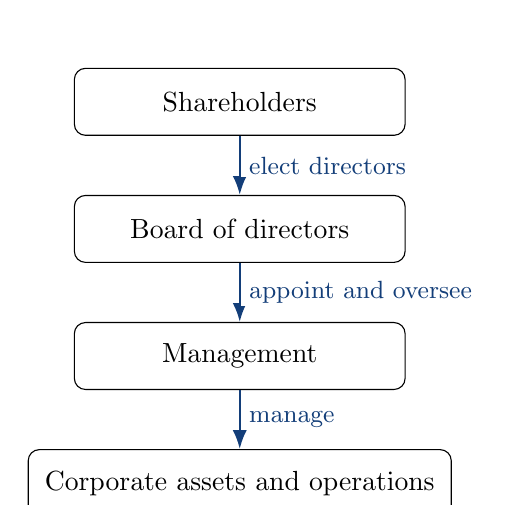
\begin{tikzpicture}[
  >=Latex,
  box/.style={
    draw,
    rounded corners,
    align=center,
    minimum width=4.2cm,
    minimum height=0.85cm,
    inner xsep=6pt,
    inner ysep=4pt,
    font=\normalsize
  },
  flow/.style={
    -Latex,
    line width=0.85pt,
    FinanceBlue
  },
  lab/.style={
    font=\small,
    text=FinanceBlue,
    fill=white,
    inner xsep=3pt,
    inner ysep=1pt
  },
  node distance=0.75cm
]

\node[box] (share) {Shareholders};

\node[box, below=of share] (board)
  {Board of directors};

\node[box, below=of board] (mgmt)
  {Management};

\node[box, below=of mgmt] (assets)
  {Corporate assets and operations};

\draw[flow]
  (share) --
  node[lab, right] {elect directors}
  (board);

\draw[flow]
  (board) --
  node[lab, right] {appoint and oversee}
  (mgmt);

\draw[flow]
  (mgmt) --
  node[lab, right] {manage}
  (assets);

\end{tikzpicture}

\caption{A simplified chain of delegated control}
\label{fig:ch9-governance-chain}
\end{figure}

Under a one-share, one-vote structure, formal voting
power is proportional to the number of voting shares
held. A shareholder holding 30\% of the
outstanding voting shares therefore holds 30\%
of the associated voting rights.Effective influence, however, also depends on ownership concentration, voter participation, voting agreements, board-election rules, and the matters subject to shareholder approval.

Voting rights have economic value when they enable
shareholders to influence corporate decisions.
A shareholder with a minority economic interest
may still exercise substantial influence when
ownership is widely dispersed and other shareholders
participate less actively in voting. The distribution
of voting rights therefore need not translate directly
into the distribution of effective control.

\subsection{Agency Problems and Ownership Structure}

Agency problems arise when decision authority is delegated and the interests of decision makers and claimants do not fully coincide. In listed corporations, ownership structure affects both the incentives to monitor corporate decisions and the conflicts that may arise from control. Two relationships are especially important.

The first is between managers and shareholders. Managers control corporate resources but may hold only a small fraction of the residual cash-flow rights. Their objectives may therefore differ from those of shareholders. Managers may value private benefits, organizational expansion, greater job security, or lower personal risk even when these choices reduce shareholder value.

Dispersed ownership can weaken monitoring incentives. A small shareholder may bear much of the cost of investigating management while receiving only a small fraction of any resulting improvement in firm value. Other shareholders can benefit from the same monitoring without bearing its cost. This free-rider problem can reduce individual incentives to monitor and increase the importance of boards, institutional investors, disclosure, auditing, and other governance mechanisms.

The second relationship is between controlling and
minority shareholders. Concentrated ownership changes
monitoring incentives. A large shareholder captures
a greater share of the benefits from improved
monitoring and may therefore have a stronger
incentive to oversee management. Greater concentration,
however, can create conflicts between controlling
and minority shareholders. A controlling shareholder
may influence related-party transactions, asset
transfers, financing decisions, or other corporate
actions in ways that provide private benefits while
reducing value for minority investors.


\begin{table}[H]

\centering

\caption{Two important equity agency problems}

\label{tab:ch9-agency-problems}

\begin{tabularx}{\textwidth}{@{}p{3.0cm}Y Y@{}}

\toprule

\textbf{Agency problem} & \textbf{Source of conflict} & \textbf{Potential governance responses} \\

\midrule

Managers versus shareholders
& Managers exercise decision authority but may hold only part of the residual claim
& Board oversight, compensation design, disclosure, monitoring, voting, takeover pressure \\

Controlling versus minority shareholders
& Controlling shareholders can influence decisions whose effects are shared with minority investors
& Related-party transaction rules, independent directors, disclosure, voting safeguards, legal protection \\

\bottomrule

\end{tabularx}

\end{table}


\subsection{Shareholder Rights and Share Classes}

A share represents a bundle of financial and governance
rights. The rights attached to a particular share depend
on corporate law, the firm's governing documents, and
the relevant share class. Differences across share
classes can affect both the distribution of financial
benefits and the allocation of voting power.

Share classes can allocate these rights differently. Preferred shares, for example, may have priority over common shares in dividends or liquidation while carrying limited or no voting rights. They remain junior to creditor claims. Conversion, redemption, or other contractual features can give preferred shares characteristics associated with both equity and debt.

Dual-class and weighted-voting structures separate voting power from economic ownership more directly. Let class \(j\) have \(N_j\) shares outstanding and \(v_j\) votes per share. Its fraction of total voting power is

\begin{equation}
\omega_j
=
\frac{v_jN_j}{\sum_k v_kN_k}.
\label{eq:ch9-voting-power}
\end{equation}

If all classes have the same cash-flow rights per share, class \(j\)'s fraction of cash-flow ownership is

\begin{equation}
\alpha_j
=
\frac{N_j}{\sum_k N_k}.
\label{eq:ch9-cash-flow-share}
\end{equation}

When voting rights differ across classes, \(\omega_j\) and \(\alpha_j\) need not coincide.

Such structures can allow founders or other controlling
shareholders to retain voting control while raising
equity from outside investors. This may support
continuity in corporate strategy, particularly when
investment projects have long horizons. At the same
time, the separation can weaken accountability to
outside shareholders whose economic exposure may
exceed their voting influence. The governance
implications depend on the safeguards provided by
corporate law and listing rules.

\begin{tcolorbox}[
  enhanced,
  breakable,
  colback=white,
  colframe=FinanceBlue,
  boxrule=0.7pt,
  sharp corners,
  borderline west={2.2pt}{0pt}{FinanceBlue},
  title=\textbf{Financial Perspective: Cash-Flow Rights and Voting Rights Need Not Coincide},
  coltitle=white,
  colbacktitle=FinanceBlue,
  fonttitle=\bfseries,
  before skip=1.2em,
  after skip=1.2em
]

A class of shares may account for a relatively small
fraction of a firm's total cash-flow rights while
carrying a larger fraction of its voting power.
Cash-flow rights determine participation in residual
economic value, whereas voting rights determine the
ability to influence corporate decisions.

\end{tcolorbox}

\subsection{Corporate Actions and Changes in Ownership Claims}

Corporate actions can change the cash held by the firm, the number of shares outstanding, or the distribution of rights among shareholders. Their immediate effects can be analyzed by considering whether cash enters or leaves the firm, whether shares are created or retired, and whether ownership fractions or rights change.

A new equity issue increases the number of shares outstanding and can change existing ownership fractions. Suppose a company has \(N_0\) shares outstanding and issues \(N_1\) new shares. An investor who owns \(n\) shares before the issue holds a fraction $\alpha_0=n/N_0$. If the investor does not participate in the new issue, the ownership fraction becomes $\alpha_0=n/(N_0+N_1)$  

The investor's percentage ownership is diluted. Percentage dilution, however, does not necessarily imply a loss of economic value. If new shares are issued at a fair price, the cash received by the firm increases its value by approximately the amount raised at the time of issuance. A smaller ownership fraction can therefore apply to a larger total equity value. If shares are issued at an unusually low price to selected investors, value can instead be transferred from nonparticipating shareholders to the new investors.

A rights issue allows existing shareholders to purchase new shares and can help them preserve their proportional ownership if they participate. Shareholders who do not participate may experience percentage dilution; transferable rights can provide compensation for the value of the subscription privilege.

\begin{example}{Percentage Dilution and Value Transfer}{new-equity-dilution}

A company has 80 million shares outstanding, trading at RMB~10 per share, giving a market equity value of RMB~800 million. An investor owns 8 million shares, or 10\% of the company.

The company issues 20 million new shares, and the investor does not participate. The investor's ownership fraction falls to

\[
\frac{8}{100}=8\%.
\]

If the new shares are issued at RMB~10, the company raises RMB~200 million. Assuming no other change in value, post-issue equity value becomes RMB~1 billion and the share price remains RMB~10. The investor's percentage ownership falls, but the value of the 8 million shares remains RMB~80 million.

If the new shares are instead issued to selected investors at RMB~5, the company raises only RMB~100 million. Under the same assumptions, post-issue equity value is approximately RMB~900 million, implying a share value of

\[
\frac{900}{100}=\text{RMB }9.
\]

The investor's shares are then worth approximately RMB~72 million. In this case, the below-market issue transfers value from existing shareholders to the new investors.

Percentage dilution and loss of economic value are therefore distinct. The economic effect depends on both the change in ownership fractions and the issue price.

\end{example}

Dividends and share repurchases both distribute cash from the firm to shareholders, but they affect ownership claims differently. A cash dividend transfers resources from the corporation to shareholders without changing the number of shares outstanding. If a firm pays a dividend \(D\) per share and no other relevant information arrives, the share price should fall when the share begins trading without the right to that dividend. Abstracting from taxes and market frictions,

\begin{equation}
P_{\mathrm{ex}}
\approx
P_{\mathrm{cum}}-D,
\label{eq:ch9-ex-dividend-price}
\end{equation}

where \(P_{\mathrm{cum}}\) is the price with the dividend right and \(P_{\mathrm{ex}}\) is the ex-dividend price. The shareholder receives cash while the firm's cash holdings decline.

A share repurchase also transfers cash from the firm to shareholders, but it reduces the number of shares outstanding. Shareholders who sell receive cash, while shareholders who retain their shares own a larger fraction of the remaining equity, all else equal. A repurchase can affect value through the price paid, information conveyed by the transaction, taxes, or changes in capital structure. A reduction in the number of shares alone does not create economic value.

A stock split changes the number of shares without transferring cash or changing proportional ownership. In a \(m\)-for-\(n\) split, the number of shares becomes

\begin{equation}
N'=\frac{m}{n}N,
\label{eq:ch9-stock-split-shares}
\end{equation}
and, absent other effects, the price per share adjusts approximately to

\begin{equation}
P'=\frac{n}{m}\times P.
\label{eq:ch9-stock-split-price}
\end{equation}

Total market capitalization therefore remains unchanged if the split conveys no new information and does not otherwise affect value.

\begin{table}[H]
\centering

\caption{Selected Corporate Actions and Their Immediate Claim-Level Effects}
\label{tab:ch9-corporate-actions}

\begin{tabularx}{\textwidth}{@{}p{2.8cm}Y Y@{}}

\toprule

\textbf{Action}
& \textbf{Immediate change}
& \textbf{Key economic question} \\

\midrule

Cash dividend
& Cash is distributed to shareholders; shares outstanding remain unchanged. The share price typically adjusts downward on the ex-dividend date.
& How does the distribution affect the resources retained by the firm and shareholder value? \\

Share repurchase
& Cash leaves the firm and shares outstanding generally decline.
& At what price are shares repurchased, and how are ownership fractions and shareholder value affected? \\

Stock split
& Shares outstanding increase and the price per share adjusts proportionally; total equity value and ownership fractions remain unchanged, other things equal.
& Does the split convey information or affect trading conditions? \\

New equity issue
& Cash enters the firm and shares outstanding increase, potentially diluting existing shareholders' ownership percentages.
& At what price are new shares issued, and how does the issue affect existing shareholders' economic value? \\

\bottomrule

\end{tabularx}

\end{table}

\section{Stock Market Architecture and Price Discovery}

Stock markets perform two linked functions. Primary markets allow firms to raise equity capital, while secondary markets allow existing shares to be transferred among investors. In secondary trading, competing buy and sell orders based on investors' information and expectations generate market prices, supported by exchanges, brokers, clearing systems, and depositories.

\subsection{Equity Issuance and Primary Markets}

A company raises new equity capital in the primary market by issuing shares to investors. An initial public offering (IPO) offers shares to public investors for the first time, while a seasoned equity offering raises additional public equity after listing. Rights issues and private placements provide other channels for issuing new shares.

Equity issuance requires the terms and price of the new claim to be determined. The issuer decides how many shares to offer and what rights they carry, while investors assess the firm's expected cash flows, risks, governance, and use of proceeds. Intermediaries such as underwriters, bookrunners, and financial advisers can support due diligence, disclosure, bookbuilding, and placement. Their role is to facilitate the issuance process and match new shares with investor demand.

A public offering may contain both primary and secondary shares. Primary shares are newly issued by the company and bring new funds into the firm. Secondary shares are sold by existing shareholders and transfer ownership without providing sale proceeds to the company. The distinction is important when interpreting the amount of capital raised by an offering.

\begin{figure}[H]
\centering

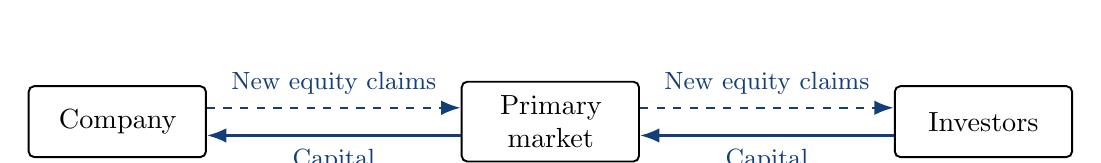
\begin{tikzpicture}[
  >=Latex,
  box/.style={
    draw,
    rounded corners=2pt,
    line width=0.7pt,
    align=center,
    text width=1.9cm,
    minimum height=0.9cm,
    inner sep=5pt
  },
  cash/.style={
    -Latex,
    line width=0.9pt,
    FinanceBlue
  },
  claim/.style={
    -Latex,
    dashed,
    line width=0.9pt,
    FinanceBlue
  },
  lab/.style={
    font=\small,
    align=center,
    fill=white,
    inner sep=1.5pt
  }
]

% Participants
\node[box] (firm) at (-1.0,0)
  {Company};

\node[box] (market) at (4.5,0)
  {Primary market};

\node[box] (investors) at (10.0,0)
  {Investors};

% New equity claims: company to investors
\draw[claim]
  ([yshift=5pt]firm.east) --
  node[lab, above=3pt] {New equity claims}
  ([yshift=5pt]market.west);

\draw[claim]
  ([yshift=5pt]market.east) --
  node[lab, above=3pt] {New equity claims}
  ([yshift=5pt]investors.west);

% Capital: investors to company
\draw[cash]
  ([yshift=-5pt]investors.west) --
  node[lab, below=3pt] {Capital}
  ([yshift=-5pt]market.east);

\draw[cash]
  ([yshift=-5pt]market.west) --
  node[lab, below=3pt] {Capital}
  ([yshift=-5pt]firm.east);

\end{tikzpicture}

\caption{Capital and Equity Claim Flows in the Primary Market}
\label{fig:ch9-primary-equity}
\end{figure}

The offer price affects the amount of capital raised
and the allocation of ownership between existing and
new shareholders. If the price is set too high relative
to investors' valuations, the offering may attract
insufficient demand. If it is set too low, the issuer
may raise less capital than it could otherwise obtain.
An initial pricing discount may reflect valuation
uncertainty, information asymmetry, and placement risk.

\subsection{Exchanges and Alternative Trading Venues}

An exchange provides rules and infrastructure for listing and trading securities. Listing and trading are related but distinct. A company may be listed on one exchange while transactions in its shares also occur through other permitted trading venues.

Organized exchanges bring orders together under
common trading rules, access arrangements, and
market-data systems. Modern equity markets may
also include alternative trading systems, such as
crossing networks and dark pools, as well as
dealer-based trading venues.

Consider a company whose shares are listed on the
New York Stock Exchange (NYSE). Investors do not
necessarily have to trade these shares on the NYSE.
Depending on applicable rules and order-routing
arrangements, a broker may execute an order on
another exchange or through an alternative trading
system (ATS), such as a dark pool. The same shares
can therefore be traded across multiple venues,
each with its own order flow and available liquidity.

Multiple venues can increase competition in execution services and allow different trading mechanisms to coexist. They can also fragment order flow, making available liquidity more difficult to observe across the market. Venue structure therefore affects how orders interact, where liquidity is concentrated, and how prices are formed.

Trading venues operate within a broader market
infrastructure. Brokers route orders, clearing
arrangements establish and, where applicable,
net the obligations arising from trades, while
securities depositories maintain ownership records
and settlement systems complete the transfer of
cash and securities. Electronic trading has changed
the speed and organization of these processes
without changing their basic economic functions.

\subsection{Trading Mechanisms, Orders, and Market Liquidity}

A trading mechanism determines how buy and sell orders interact. In an order-driven market, orders are submitted to a limit order book and transactions occur when compatible orders meet. In a dealer market, dealers quote prices at which they are willing to buy and sell. Many modern equity markets combine elements of these structures.

A market order gives priority to execution at the best available prices, subject to available quantity. A limit order specifies the highest price a buyer is willing to pay or the lowest price a seller is willing to accept. It provides greater price control but may remain unexecuted. Market orders typically demand available liquidity, while nonmarketable limit orders can supply liquidity to other traders.

If the best bid and ask are \(P_{\mathrm{bid}}\) and \(P_{\mathrm{ask}}\), the quoted bid--ask spread is

\begin{equation*}
s=P_{\mathrm{ask}}-P_{\mathrm{bid}}.
\label{eq:ch9-bid-ask-spread}
\end{equation*}

The midpoint is

\begin{equation*}
M=\frac{P_{\mathrm{ask}}+P_{\mathrm{bid}}}{2},
\label{eq:ch9-midquote}
\end{equation*}
and the proportional quoted spread is

\begin{equation*}
s_{\mathrm{rel}}
=
\frac{P_{\mathrm{ask}}-P_{\mathrm{bid}}}{M}.
\label{eq:ch9-relative-spread}
\end{equation*}

The spread is one dimension of liquidity. Depth measures the quantity available near current prices, while price impact describes how strongly execution prices respond to order size. A market can display a narrow spread for small trades while offering limited depth for larger orders.

The supply of liquidity can vary with market conditions. When uncertainty or adverse-selection risk increases, liquidity suppliers may quote wider spreads, display less depth, or withdraw orders. The possibility of trading against better-informed investors therefore links information conditions to market liquidity.

Trading constraints also affect how information and investor views enter the order flow. Short selling allows an investor to borrow shares, sell them, and later repurchase shares to return to the lender. It enables negative information or expectations to be expressed through sell orders even when the investor does not initially own the shares. Restrictions or high borrowing costs can limit this channel. Short selling can therefore affect order flow, liquidity, and price discovery, although its effects depend on market conditions and trading rules.

\subsection{Information, Prices, and Price Discovery}

A stock price is an observed trading price for an equity claim. It can change when investors revise expectations about future cash flows or required returns, or when the rights attached to the claim change.

Let \(\mathcal{I}_t\) denote the information available at time \(t\). A dividend-based valuation benchmark can be written as

\begin{equation}
P_t
=
\sum_{j=1}^{\infty}
\frac{\mathrm{E}[D_{t+j}\mid\mathcal{I}_t]}
{(1+r_{e,t})^j},
\label{eq:ch9-information-price}
\end{equation}
where \(r_{e,t}\) is treated as a constant required return from time \(t\) onward. New information can change expected future dividends, the required return, or both, and therefore change the value investors assign to the share.

Price discovery is the process through which information and investor assessments are reflected in market prices through trading. Investors may differ in their information, models, expectations, and liquidity needs, so their orders reveal only part of what they know. Price discovery can therefore be informative without being instantaneous or costless. Figure~\ref{fig:ch9-price-discovery} summarizes
the process through which information and investor
assessments are reflected in observed market prices,
with market frictions affecting this process.


\begin{figure}[H]

\centering

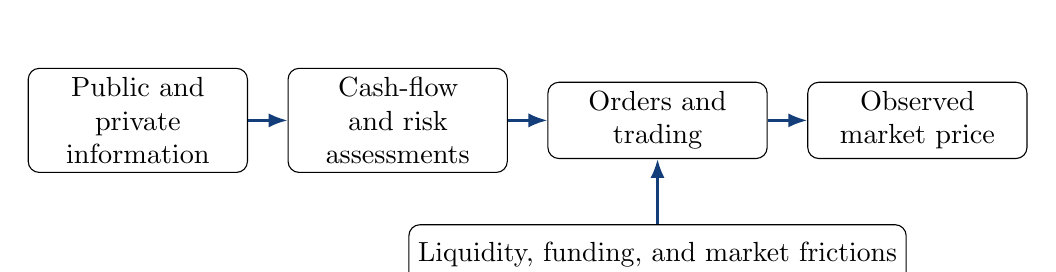
\begin{tikzpicture}[
  >=Latex,
  box/.style={
    draw,
    rounded corners,
    align=center,
    text width=2.55cm,
    minimum height=0.9cm
  },
  flow/.style={
    -Latex,
    line width=0.85pt,
    FinanceBlue
  }
]

\node[box] (info) at (0,1.4)
  {Public and private\\information};

\node[box] (beliefs) at (3.3,1.4)
  {Cash-flow and risk\\assessments};

\node[box] (orders) at (6.6,1.4)
  {Orders and\\trading};

\node[box] (price) at (9.9,1.4)
  {Observed\\market price};

\draw[flow] (info) -- (beliefs);
\draw[flow] (beliefs) -- (orders);
\draw[flow] (orders) -- (price);

\node[
  draw,
  rounded corners,
  align=center,
  minimum width=5.8cm,
  minimum height=0.75cm
] (frictions) at (6.6,-0.3)
  {Liquidity, funding, and market frictions};

\draw[flow] (frictions.north) -- (orders.south);

\end{tikzpicture}

\caption{Information, trading, and price discovery}
\label{fig:ch9-price-discovery}
\end{figure}

The efficient-market hypothesis provides a benchmark
for evaluating how information is incorporated into
market prices. Its implications depend on the
information set considered. Under the hypothesis,
investors should not be able to generate abnormal
risk-adjusted returns systematically using the
information covered by the relevant form of market
efficiency, after accounting for transaction and
information costs.

The hypothesis is commonly expressed in three forms according to the information set considered. Weak-form efficiency concerns information contained in past prices and trading activity. Semi-strong-form efficiency extends the information set to publicly available information, including financial reports and corporate announcements. Strong-form efficiency considers both public and private information and is best viewed as a demanding benchmark rather than a literal description of most markets.

Price discovery remains subject to economic frictions. Information can be costly to acquire, investors can disagree, and liquidity conditions, funding constraints, and limits to arbitrage can affect observed prices. If prices fully revealed all costly-to-acquire
information, investors would have little incentive
to incur the costs of acquiring it.

\begin{tcolorbox}[
  enhanced,
  breakable,
  colback=white,
  colframe=FinanceBlue,
  boxrule=0.7pt,
  sharp corners,
  borderline west={2.2pt}{0pt}{FinanceBlue},
  title=\textbf{Financial Perspective: Price Discovery Is Not Perfect Valuation},
  coltitle=white,
  colbacktitle=FinanceBlue,
  fonttitle=\bfseries,
  before skip=1.2em,
  after skip=1.2em
]

Observed market prices reflect investors' information,
expectations, and assessments under prevailing market
conditions. They provide signals about economic value,
but are not direct observations of an objectively
known fundamental value.

\end{tcolorbox}

\section{Equity Value and Risk}

Equity value reflects the present value of the cash flows available to shareholders, adjusted for the risk of those cash flows. Three elements are central to equity valuation: expected shareholder cash flows, the effect of reinvestment on future growth, and a required return consistent with equity risk.

\subsection{Equity Cash Flows and Valuation Inputs}

A distinction should be made between book equity and
market equity. Book equity is an accounting measure
derived from recognized assets and liabilities,
whereas market equity is the market value of
outstanding equity claims. The two need not coincide,
since market value reflects expectations about future
cash flows, growth opportunities, risk, and the rights
attached to the shares.

Dividends are direct cash payments from the corporation to shareholders. Share repurchases provide another form of payout: cash is paid to shareholders who sell their shares, while the number of shares outstanding declines. Dividends and repurchases therefore distribute value in different ways.

Retained earnings are not a distribution to shareholders when they are retained. Their contribution to equity value depends on the future cash flows generated by the resources kept within the firm. Retention creates value only to the extent that reinvestment supports sufficiently valuable future cash flows.

For an investor who plans to hold a share through date \(T\), the value today can be expressed as the present value of expected dividends during the holding period and the expected sale price:

\begin{equation}
P_0
=
\sum_{t=1}^{T}
\frac{\mathrm{E}[D_t]}{(1+r_e)^t}
+
\frac{\mathrm{E}[P_T]}{(1+r_e)^T},
\label{eq:ch9-finite-horizon-equity-value}
\end{equation}
where \(r_e\) is the required return on the equity claim under a constant-rate simplification.

If the terminal price is valued as the present value
of expected dividends beyond date $T$, extending
the valuation horizon indefinitely gives the
dividend discount representation:

\begin{equation}
P_0
=
\sum_{t=1}^{\infty}
\frac{\mathrm{E}[D_t]}{(1+r_e)^t}.
\label{eq:ch9-dividend-discount-model}
\end{equation}


For total equity valuation, analysts may instead forecast free cash flow to equity, \(FCFE_t\), the cash flow available to equity holders after operating needs, taxes, reinvestment, and net debt financing. A simplified valuation expression is

\begin{equation}
V_E
=
\sum_{t=1}^{\infty}
\frac{\mathrm{E}[FCFE_t]}{(1+r_e)^t}.
\label{eq:ch9-fcfe-valuation}
\end{equation}

The cash-flow measure and discount rate should refer to the same claim. Cash flows available to all capital providers require a discount rate appropriate to the entire enterprise, while cash flows available only to equity holders require an equity required return.

Market prices of comparable firms provide additional valuation benchmarks. Relative valuation uses measures such as price--earnings and price--book ratios to compare similar equity claims. Such comparisons are more informative when differences in growth, profitability, leverage, risk, and accounting measurement are taken into account.

\subsection{Growth Expectations and Market Value}

Growth affects equity value through its effect on future cash flows and the reinvestment required to generate them. Higher expected sales or earnings do not by themselves imply higher value. Reinvestment creates value when the return earned on additional equity exceeds the return required by shareholders.

The dividend payout ratio links expected earnings
to the next-period dividend. Suppose next-period
earnings per share are $E_1$, the firm retains a
fraction $k$ of earnings, and distributes the
remainder as dividends. Then

\begin{equation}
D_1=(1-k)E_1.
\label{eq:ch9-dividend-payout}
\end{equation}

If growth is financed through retained earnings, no
net new common equity is issued, and the return on
beginning book equity remains stable, a simplified
sustainable growth relation is

\begin{equation}
g=k\,ROE.
\label{eq:ch9-sustainable-growth}
\end{equation}

If dividends are expected to grow at a constant rate
$g$ indefinitely, the Gordon growth model, also known
as the constant-growth dividend discount model,
expresses the current share price as

\begin{equation}
P_0=\frac{D_1}{r_e-g},
\qquad
r_e>g.
\label{eq:ch9-gordon-growth}
\end{equation}

Substituting the payout and growth relations gives

\begin{equation}
P_0
=
\frac{(1-k)E_1}
{r_e-k\,ROE}.
\label{eq:ch9-growth-reinvestment-value}
\end{equation}

A higher retention ratio reduces current payout but can increase future growth. Its effect on value depends on the return earned on the retained resources relative to the required return on equity.

\begin{example}{Growth and Value Creation}{growth-reinvestment-value}

Suppose next-period earnings per share are 10, the retention ratio is 40\%, and the required return on equity is 10\%.

If retained earnings earn a stable \(ROE\) of 15\%,

\[
g=0.40\times 0.15=6\%,
\]
and
\[
P_0=\frac{(1-0.40)\times 10}{0.10-0.06}=\frac{6}{0.04}=150.
\]

If the return on equity is instead 8\%,

\[
g=0.40\times 0.08=3.2\%,
\]
and
\[
P_0=\frac{(1-0.40)\times 10}{0.10-0.032}=\frac{6}{0.068}\approx88.24.
\]

In this simplified setting, growth adds value when reinvestment earns more than the required return and reduces value when it earns less.

\end{example}

The same principle extends beyond constant-growth models. Rapid growth can require substantial investment, while modest current payout can be consistent with high value when retained resources are expected to generate sufficiently strong future cash flows. Growth expectations can also affect the timing of value. When a larger share of expected cash flows lies further in the future, equity value becomes more sensitive to changes in the required return.

\begin{tcolorbox}[
  enhanced,
  breakable,
  colback=white,
  colframe=FinanceBlue,
  boxrule=0.7pt,
  sharp corners,
  borderline west={2.2pt}{0pt}{FinanceBlue},
  title=\textbf{Financial Perspective: Growth Is Not the Same as Value Creation},
  coltitle=white,
  colbacktitle=FinanceBlue,
  fonttitle=\bfseries,
  before skip=1.2em,
  after skip=1.2em
]

Growth increases equity value only when the returns generated by the required reinvestment are sufficient relative to the return required by shareholders.

\end{tcolorbox}

\subsection{Equity Risk Premium and Required Return}

An investor's realized return on a share over one period combines the dividend received and the change in market price. If the initial price is \(P_0\), the end-of-period price is \(P_1\), and the dividend is \(D_1\), the realized holding-period return is

\begin{equation}
r
=
\frac{P_1-P_0+D_1}{P_0}.
\label{eq:ch9-equity-realized-return}
\end{equation}

A required return is different from a realized return. It is the return investors require for holding an equity claim given its risk and the returns available on alternative investments. Risks that can be diversified across many investments generally require less compensation than risks associated with broad economic conditions.

Let \(r_M\) denote the return on a broad market portfolio and \(r_f\) the risk-free rate. The market equity risk premium is

\begin{equation}
ERP
=
\mathrm{E}[r_M]-r_f.
\label{eq:ch9-equity-risk-premium}
\end{equation}

The equity risk premium is forward-looking. Historical averages of realized stock returns over risk-free returns can provide evidence about past outcomes, but they need not equal the premium investors require at a particular date.

The Capital Asset Pricing Model provides a widely used benchmark for relating a stock's required return to systematic risk. The beta of stock \(i\) is

\begin{equation}
\beta_i
=
\frac{\mathrm{Cov}(r_i,r_M)}
{\mathrm{Var}(r_M)}.
\label{eq:ch9-beta}
\end{equation}

Under the CAPM assumptions, the required return is

\begin{equation}
r_i
=
r_f
+
\beta_i\left(\mathrm{E}[r_M]-r_f\right).
\label{eq:ch9-capm}
\end{equation}

Beta measures the stock's exposure to market-wide return movements. A higher beta implies a larger required risk premium within the CAPM.

\begin{example}{A CAPM Required Return}{capm-required-return}

Suppose the risk-free rate is 3\%, the expected market equity risk premium is 6\%, and a stock has a beta of 1.2. The CAPM required return is

\[
r_i
=
3\%+1.2(6\%)
=
10.2\%.
\]

The estimate is conditional on the CAPM and on the inputs used.

\end{example}
The CAPM is a benchmark rather than a complete description of expected returns. Its broader economic insight is that risks linked to adverse market-wide conditions tend to require greater compensation because they are difficult to diversify when protection is most valuable. Beta represents this exposure through covariance with the market, while other asset-pricing models allow for additional sources of priced risk.

%========================================================
% Summary
%========================================================

\TailModule{summary}{Summary}

Common equity is a residual ownership claim. Shareholders receive value after senior contractual claims are satisfied and participate in the remaining upside, while limited liability ordinarily prevents losses on a fully paid share from extending beyond the value invested in that share. Equity financing provides capital without creating fixed contractual interest or principal payments and gives new investors residual cash-flow rights and, usually, voting rights. New issuance can dilute percentage ownership even when it increases the resources available to the firm.

Corporate governance allocates control over corporate resources. Shareholders usually exercise control indirectly through voting and the election of directors, while boards appoint and oversee management. Dispersed ownership can weaken monitoring incentives, whereas concentrated ownership can strengthen monitoring while increasing potential conflicts between controlling and minority shareholders. Share classes can separate cash-flow rights from voting rights, and corporate actions such as dividends, repurchases, stock splits, and new issues affect cash, share counts, and ownership claims in different ways.

Stock markets perform both financing and trading functions. Primary issues can bring new capital into the company, while secondary trades transfer existing shares among investors. Exchanges and other trading venues provide mechanisms through which orders interact, while liquidity depends on spreads, depth, price impact, information conditions, and the willingness of market participants to supply liquidity. Price discovery reflects information, expectations, risk assessments, and liquidity conditions in observable market prices through trading, without implying that every observed price equals an objectively known fundamental value.

Equity valuation requires consistency between shareholder cash flows and the required return used to discount them. Dividends and repurchases distribute cash, while retained earnings contribute to value through the future cash flows generated by reinvestment. Growth increases value when reinvestment is expected to earn sufficiently high returns relative to the required return on equity. The market equity risk premium represents the expected excess return on broad equity exposure, while the CAPM provides a benchmark linking an individual stock's required return to its systematic risk.

%========================================================
% Key Terms
%========================================================

\TailModule{keyterms}{Key Terms}

Common equity; residual claim; limited liability; ownership dilution; voting rights; board of directors; corporate governance; agency problem; controlling shareholder; minority shareholder; share class; preferred share; weighted voting rights; cash dividend; share repurchase; stock split; rights issue; initial public offering; seasoned equity offering; primary shares; secondary shares; exchange; alternative trading venue; market order; limit order; bid--ask spread; market liquidity; price discovery; informational efficiency; dividend discount model; free cash flow to equity; retention ratio; sustainable growth; equity risk premium; beta; Capital asset pricing model.

%========================================================
% Financial AI Lab
%========================================================

\TailModule{aiprompt}{Financial AI Lab}

\textbf{Lab: Audit an AI Equity Valuation and Governance Comparison}

Choose two publicly listed companies in the same broad industry. Ask an AI system to compare their equity valuations using a simple price multiple and either a free-cash-flow-to-equity or dividend-based approach. Require the system to identify the share class being valued, the relevant number of shares outstanding, the expected growth assumptions, the required return, and the source of each factual input.

Audit the result in four stages.

\begin{enumerate}

\item Verify whether the market capitalization and per-share valuation use the appropriate share count and whether each valuation multiple is matched to the corresponding equity measure.

\item Examine how the valuation responds to assumptions about growth and the required return. Test at least one alternative growth rate and one alternative required return or, when applicable, equity risk premium.

\item Compare the voting and cash-flow rights attached to the selected share classes. Determine whether one-share, one-vote applies or whether the governance structure separates voting power from economic ownership.

\item Check each factual claim against company disclosures or an official exchange source. Identify at least one statement for which the AI provides a plausible interpretation but insufficient supporting evidence.

\end{enumerate}

%========================================================
% Discussion Questions
%========================================================

\TailModule{questions}{Discussion Questions}

\begin{enumerate}

\item Why does limited liability not make common equity a low-risk claim? Distinguish between the maximum loss arising from ownership of the share itself and variation in the share's market value.

\item How can concentrated ownership reduce one agency problem while increasing another?

\item Why can a stock price rise sharply after favorable news even when no new cash enters the company from the stock market?

\item Why does faster earnings growth not necessarily imply a higher equity value? Relate your answer to reinvestment and the required return on equity.

\item Why should a historical average of realized market returns in excess of risk-free returns not be treated automatically as the current expected equity risk premium?

\end{enumerate}

%========================================================
% Applied Problems
%========================================================

\TailModule{appprobs}{Applied Problems}

\begin{enumerate}

\item \textbf{Residual payoffs and limited liability.}

A firm financed with debt and common equity will generate cash flow of either 160 or 70 next period, with each state equally likely. Promised debt repayment is 100.

\begin{enumerate}

\item Calculate the debt and equity payoffs in each state.

\item Calculate the expected payoff to equity.

\item Explain which part of the equity payoff structure reflects limited liability.

\item Explain why shareholders may benefit from a shift toward a riskier distribution of firm cash flows after debt has been issued, while creditors may lose.

\end{enumerate}

\item \textbf{Voting power and cash-flow ownership.}

A company has 20 million Class A shares with 10 votes
per share and 180 million Class B shares with one vote
per share. Assume that the two classes have identical
cash-flow rights per share.

\begin{enumerate}

\item Calculate the Class A share of the firm's total
cash-flow rights.

\item Calculate the Class A share of total voting power.

\item Explain why the two percentages differ.

\item Identify one potential benefit and one potential
governance risk of this structure.

\end{enumerate}

\item \textbf{Market and limit orders.}

The best bid for a stock is 24.96 for 6,000 shares and the best ask is 25.04 for 4,000 shares.

\begin{enumerate}

\item Calculate the quoted spread and midpoint.

\item Calculate the proportional quoted spread.

\item At what price can a market order to buy 2,000 shares execute if the quotation remains available?

\item If a limit order to buy 2,000 shares at 25.00 is submitted and no seller is willing to sell at 25.00 or below, how is the order treated in the limit order book?

\end{enumerate}

\item \textbf{Growth and reinvestment.}

A company expects next-period earnings per share of 8 and has a required return on equity of 11\%. The firm retains 30\% of earnings. Assume that growth is financed through retained earnings, no net new common equity is issued, and \(ROE\) remains stable at 16\%.

\begin{enumerate}

\item Calculate the sustainable growth rate.

\item Calculate next-period dividends per share.

\item Using the constant-growth model, calculate the share value.

\item Recalculate the value if \(ROE\) falls to 9\% while the retention ratio remains unchanged.

\item Explain the direction of the valuation change.

\end{enumerate}

\item \textbf{Equity risk and required return.}

The risk-free rate is 2.5\% and the expected market equity risk premium is 5.5\%.

\begin{enumerate}

\item Calculate the CAPM required return for a stock with beta 0.8.

\item Calculate the required return for a stock with beta 1.4.

\item Explain why the higher-beta stock has the higher required return within the CAPM.

\item Give one reason why an analyst might not want to rely on the CAPM estimate alone.

\end{enumerate}

\end{enumerate}

%========================================================
% Data Application
%========================================================

\TailModule{dataapp}{Data Application}

\textbf{Information and Price Discovery in China's Equity Market}

Select one A-share company listed on the Shanghai Stock Exchange or Shenzhen Stock Exchange and identify a dated corporate disclosure containing economically relevant new information, such as an earnings announcement, profit warning, major investment decision, dividend proposal, share repurchase plan, or new equity issue. Use the exchange disclosure platform and the company's formal announcement as the primary sources for the disclosure.

Collect the stock's daily closing prices for several trading days before and after the disclosure, together with a broad market index over the same period. Calculate daily stock returns and a simple market-adjusted abnormal return

\begin{equation*}
r_t=r_{i,t}-r_{M,t},
\end{equation*}

where \(r_{i,t}\) is the stock return and \(r_{M,t}\) is the market-index return on day \(t\).

Identify the exact time at which the information first became publicly available. If the disclosure was released after the market closed, treat the next trading day as the first day on which investors could respond through trading. Plot the stock price and report the market-adjusted returns around the disclosure. Determine whether the largest price movement occurred before, on, or after the first trading opportunity following the disclosure.

Interpret the result cautiously. A price reaction can reflect revisions to expected cash flows, required returns, or both. Market-wide news and other firm-specific information released near the same time can also affect observed returns. A short event window and daily closing prices do not by themselves establish causality or the speed of intraday price discovery.

Report the company, stock code, disclosure title, disclosure date and time, sample period, benchmark index, and data sources. Explain what additional evidence would be needed before concluding that the market anticipated the information, reacted slowly, or overreacted.

%========================================================
% Case Analysis
%========================================================

\TailModule{caseanalysis}{Case Analysis}

\CaseLabel{Historical Case Based on Public Information}

\textbf{Case: Xiaomi and Weighted Voting Rights in Hong Kong}

Xiaomi Corporation began trading in Hong Kong on July 9, 2018 and became the first company to list there with a weighted voting rights structure after the 2018 listing-regime reforms. Xiaomi's Class A shares carry ten votes per share on most shareholder resolutions, while Class B shares carry one vote per share. For specified reserved matters, each share carries one vote. The publicly listed shares are Class B shares.\footnote{Xiaomi Corporation, \emph{Global Offering Prospectus}, June 2018, \url{https://www1.hkexnews.hk/listedco/listconews/sehk/2018/0625/ltn20180625033.pdf}.}

The structure separates voting power from economic ownership. It can allow founders to retain substantial influence over corporate decisions after raising equity from public investors. Hong Kong's listing rules permit specified weighted-voting structures subject to eligibility requirements, continuing obligations, and safeguards for non-weighted-voting shareholders.

Analyze the structure from both financing and governance perspectives. Why might founders value the ability to raise public equity without surrendering proportional voting control? How could concentrated voting power support strategic continuity or long-horizon investment? What agency problems can arise when voting control exceeds cash-flow ownership? Which investor-protection mechanisms become more important when outside shareholders have weaker voting power?

Then consider the market-value implications. Explain why the market price of Xiaomi's publicly traded Class B shares reflects not only expected residual cash flows but also the governance rights and control structure associated with the investment. Would a change in voting rights necessarily leave market value unchanged if expected operating cash flows were initially unaffected? Explain how changes in control, agency costs, future cash-flow allocation, or the required return could affect equity value.

\emph{Primary sources: Hong Kong Exchanges and Clearing Limited, ``HKEX to Offer Investors More Options When Xiaomi Shares Debut,'' July 4, 2018; Xiaomi Corporation, 2018 Prospectus and 2018 Interim Report; Hong Kong Stock Exchange Listing Rules, Chapter 8A on Weighted Voting Rights.}

%========================================================
% Further Reading
%========================================================

\TailModule{furtherread}{Further Reading}

\begin{itemize}

\item Gordon, Myron J. (1959),
``Dividends, Earnings, and Stock Prices,''
\emph{The Review of Economics and Statistics}, 41(2, Part 1), 99--105.

\item Fama, Eugene F. (1970),
``Efficient Capital Markets: A Review of Theory and Empirical Work,''
\emph{The Journal of Finance}, 25(2), 383--417.

\item Grossman, Sanford J., and Joseph E. Stiglitz (1980),
``On the Impossibility of Informationally Efficient Markets,''
\emph{American Economic Review}, 70(3), 393--408.

\item Kyle, Albert S. (1985),
``Continuous Auctions and Insider Trading,''
\emph{Econometrica}, 53(6), 1315--1335.

\item La Porta, Rafael, Florencio Lopez-de-Silanes, Andrei Shleifer, and Robert W. Vishny (2000),
``Investor Protection and Corporate Governance,''
\emph{Journal of Financial Economics}, 58(1--2), 3--27.

\end{itemize}

\ChapterTail{summary,keyterms,aiprompt,questions,appprobs,dataapp,caseanalysis,furtherread}

\chapter{Foreign Exchange Markets and Cross-Border Finance}
\label{chap:Foreign_Exchange_Markets_and_Cross_Border_Finance}

\begin{openingcase}{How Much Is a Foreign-Currency Receivable Worth?}

A Chinese manufacturer has sold equipment to an overseas customer for USD~10 million, payable in three months. At today's spot exchange rate of RMB~7.20 per U.S. dollar, the receivable is worth RMB~72 million. But the company will receive the dollars only in three months, when the spot exchange rate may be different.

The firm can leave the currency exposure open and convert the dollars when payment arrives, or sell the future dollar receipts forward and lock in an exchange rate today. The sales contract determines the dollar cash flow; the foreign exchange market determines its RMB value and how the exchange-rate risk is allocated.

\end{openingcase}

\begin{tcolorbox}[
  enhanced,
  colback=FinanceBlue!6,
  colframe=FinanceBlue,
  boxrule=0.6pt,
  sharp corners,
  left=8pt,
  right=8pt,
  top=7pt,
  bottom=7pt,
  before skip=1em,
  after skip=1.6em,
  title=\textbf{Core Questions},
  coltitle=white,
  colbacktitle=FinanceBlue,
  fonttitle=\bfseries,
  attach boxed title to top left={xshift=6pt,yshift=-2mm},
  boxed title style={
    boxrule=0pt,
    sharp corners,
    left=5pt,
    right=5pt,
    top=2pt,
    bottom=2pt
  }
]
\begin{enumerate}[
  leftmargin=*,
  label=\textcolor{FinanceBlue}{\textbf{\arabic*.}},
  itemsep=0.55em,
  topsep=0.2em
]

\item How do foreign exchange markets connect
international trade, investment, and cross-border
funding when cash flows are denominated in different
currencies?

\item How are spot exchange rates formed through
currency demand and supply, and how do capital flows,
expectations, and market liquidity influence
exchange-rate movements and price discovery?

\item How are spot and forward exchange rates linked
through interest-rate differentials and covered
interest parity, and how can firms and investors
use foreign exchange instruments to manage
exchange-rate risk?

\end{enumerate}

\end{tcolorbox}

\section{The Architecture of Foreign Exchange Markets}

An exchange rate is the price of one currency in terms
of another. Foreign exchange markets provide the
mechanisms through which cross-border payments,
investment, and funding are converted between
currencies.

\subsection{International Trade, Investment, and Funding Needs}

Cross-border transactions create currency exposure when
the denomination currency of a contractual cash flow
differs from the currency in which the relevant firm
or investor measures its value. The denomination
currency specifies the currency in which contractual
payments are expressed, whereas the valuation currency
is the currency used to measure the economic value of
the claim or liability. When these currencies differ,
the contractual amount may remain fixed while its
value in the valuation currency changes with the
exchange rate.

Let $S_t$ denote units of domestic currency per unit of foreign currency. An increase in $S_t$ therefore represents a depreciation of the domestic currency.

Suppose a domestic exporter will receive $F$ units
of foreign currency at date $T$. If the receipt is
converted at the spot exchange rate prevailing at
that date, its domestic-currency value is

\begin{equation}
V_{D,T}=S_T V_{F,T}.
\label{eq:ch10-export-receivable-value}
\end{equation}

The commercial contract fixes the foreign-currency
amount, but its domestic-currency value varies
with $S_T$. A higher $S_T$ increases the domestic-
currency value of a foreign-currency receivable.
A foreign-currency payable creates the opposite
net exposure, as a higher $S_T$ increases the
domestic-currency cost of meeting the obligation.

Cross-border investment combines foreign-asset returns with exchange-rate movements. Suppose a domestic investor converts one unit of domestic currency into foreign currency at $S_0$, earns a foreign-currency return $r^{*}$, and converts the proceeds back at $S_1$. The domestic-currency gross return is

\begin{equation}
1+r_d=(1+r^{*})\frac{S_1}{S_0}.
\label{eq:ch10-foreign-investment-return}
\end{equation}

The domestic-currency return depends on both the foreign-asset return and the change in the exchange rate. An appreciation of the domestic currency can reduce the domestic-currency value of foreign investment returns, while a depreciation can increase it.

Cross-border borrowing places currency exposure on the liability side. A foreign-currency loan may carry a lower contractual interest rate, but its domestic-currency repayment cost also depends on the future exchange rate. Comparing domestic and foreign funding therefore requires both borrowing terms and currency exposure to be considered on a common basis.

\subsection[Market Participants, Dealers, and Electronic Trading Platforms]{Market Participants, Dealers, and Electronic Trading\ Platforms}

The foreign exchange market is a decentralized network rather than a single exchange. Banks, non-bank dealers, corporations, asset managers, hedge funds, central banks, and other institutions trade through dealer networks, electronic venues, and bilateral relationships.

Participants enter the market to execute currency
conversions arising from trade, investment, and
funding transactions. Dealers intermediate these
flows by quoting exchange rates, providing immediate
execution, and managing the resulting currency
positions.

Dealer intermediation creates several layers of trading. A corporate customer may trade with a bank, while the bank can offset the resulting position against another customer flow, with another dealer, or through an electronic venue. A customer transaction may therefore lead to additional trades as currency positions are redistributed through the market.

\begin{figure}[H]
\centering

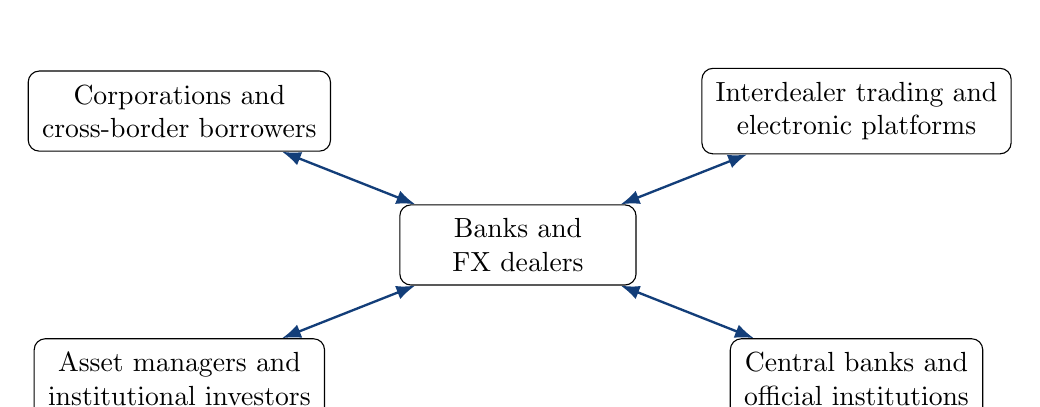
\begin{tikzpicture}[
  >=Latex,
  box/.style={
    draw,
    rounded corners,
    align=center,
    minimum width=3.0cm,
    minimum height=0.9cm,
    inner sep=5pt
  },
  two/.style={
    Latex-Latex,
    line width=0.85pt,
    FinanceBlue
  }
]

\node[box] (corp) at (-4.3,1.7)
  {Corporations and\\cross-border borrowers};

\node[box] (asset) at (-4.3,-1.7)
  {Asset managers and\\institutional investors};

\node[box] (dealer) at (0,0)
  {Banks and\\FX dealers};

\node[box] (inter) at (4.3,1.7)
  {Interdealer trading and\\electronic platforms};

\node[box] (policy) at (4.3,-1.7)
  {Central banks and\\official institutions};

\draw[two] (corp) -- (dealer);
\draw[two] (asset) -- (dealer);
\draw[two] (dealer) -- (inter);
\draw[two] (dealer) -- (policy);

\end{tikzpicture}

\caption{A simplified architecture of foreign exchange trading}
\label{fig:ch10-fx-market-architecture}
\end{figure}

The figure is schematic. Some institutional investors
and non-bank financial institutions also access
electronic trading platforms and other liquidity
providers directly. Central banks participate mainly
through official transactions, including reserve
management and foreign exchange intervention.

Electronic trading has reduced search and execution
costs in many segments of the market by allowing
quotes and orders from multiple sources to be compared
and matched more rapidly. However, large trades,
less liquid currency pairs, and customized contracts
may rely more heavily on dealer relationships and
bilateral credit arrangements.

Foreign exchange trading also creates settlement obligations. The two parties deliver different currencies, often through payment systems in different jurisdictions. If one currency is delivered before the other is received, the party that has already paid is exposed to settlement risk. Payment-versus-payment arrangements can reduce this exposure by linking the settlement of the two currency legs, although liquidity, operational, and legal risks may remain.

These institutional arrangements provide the setting
in which spot exchange rates are quoted and currency
positions are traded across the market.

\subsection{Spot Quotes, Market Liquidity, and Price Discovery}

A spot exchange rate is the price at which two currencies are exchanged under the market's standard near-term settlement convention. Settlement timing can differ across currency pairs, so the applicable settlement date remains part of the transaction terms.

Under this quotation convention, $S_t$ is a direct
quote from the perspective of a domestic participant.
The reciprocal quote is

\begin{equation}
\widetilde{S}_t=\frac{1}{S_t},
\label{eq:ch10-reciprocal-quote}
\end{equation}
measured as units of foreign currency per unit of domestic currency. If the exchange rate is RMB~7.20 per U.S. dollar, the reciprocal quote is approximately $1/7.20=0.1389$ U.S. dollars per renminbi.

The quote convention determines how exchange-rate movements are interpreted. Under a domestic-currency-per-foreign-currency quote, a rise in $S_t$ means that more domestic currency is required to purchase one unit of foreign currency. Thus, a movement from RMB~7.20 to RMB~7.40 per dollar represents a depreciation of the renminbi against the dollar.

Spot transactions are generally quoted with a bid and an ask. For a quote expressed as domestic currency per unit of foreign currency, the bid is the price at which the dealer buys the foreign currency, while the ask is the price at which the dealer sells it. If the quote is 7.1980--7.2020 RMB per dollar, the quoted spread is

\begin{equation*}
\text{Spread}=7.2020-7.1980=0.0040.
\label{eq:ch10-fx-spread}
\end{equation*}

The bid--ask spread is one dimension of market liquidity. A narrower spread generally implies a lower immediate transaction cost for a trade of the quoted size. Liquidity also depends on market depth and price impact. Depth refers to the quantity available near the current price, while price impact refers to the change in execution prices associated with larger orders. These conditions can vary across currency pairs, trading hours, market conditions, and trade sizes.

Cross rates link prices across currency pairs. Suppose the market quotes $S^{\mathrm{CNY/USD}}=7.20$ RMB per dollar and $S^{\mathrm{USD/EUR}}=1.10$ dollars per euro. The implied renminbi-per-euro cross rate is

\begin{equation*}
S^{\mathrm{CNY/EUR}}
=S^{\mathrm{CNY/USD}}\times
S^{\mathrm{USD/EUR}}
=7.92.
\label{eq:ch10-cross-rate}
\end{equation*}

Differences between directly quoted and implied cross rates can create arbitrage opportunities when they are large enough to cover transaction costs and execution constraints. Trading across related currency pairs tends to keep these prices closely aligned.

\begin{example}{Cross Rates and Triangular Arbitrage}{fx-triangular-arbitrage}

Suppose the market quotes RMB~7.20 per U.S. dollar and USD~1.10 per euro, implying a cross rate of RMB~7.92 per euro. If the direct RMB/EUR quote were RMB~8.00 per euro, the euro would be more expensive in the direct market than through the dollar.

Ignoring transaction costs, a trader could obtain euros indirectly through dollars and sell them at the higher direct RMB/EUR rate. Such transactions tend to reduce price differences across related currency pairs. In practice, the difference must be sufficient to cover bid--ask spreads and other execution costs.

\end{example}

Price discovery occurs as customer and investor
orders interact with dealer quotes. Order flow can
reveal changes in buying and selling pressure and
affect dealer inventories, prompting quote adjustments
and position reallocation. Observed exchange rates
therefore reflect the interaction of trading activity
with available liquidity and market-making capacity.

An observed exchange-rate movement may therefore reflect several forces at the same time. Changes in policy rates, inflation expectations, economic conditions, and risk perceptions can interact, so the exchange-rate response depends on how the broader information set changes expected returns across currencies.


\section{Exchange-Rate Measures, Regimes, and Dynamics}

Changes in monetary conditions, capital flows,
expectations, and risk create pressures on currency
values. How these pressures are reflected in market
exchange rates, official intervention, or other
policy adjustments depends on the exchange-rate regime.

\subsection{Nominal, Real, and Effective Exchange Rates}

The nominal exchange rate expresses the price of
one currency in terms of another, without adjusting
for differences in domestic and foreign price levels.
It converts foreign-currency prices into domestic
currency, but does not by itself determine the
relative price of domestic and foreign goods.

Let $P_t$ denote the domestic price level and $P_t^*$
the foreign price level. The term $S_tP_t^*$ converts
the foreign price level into domestic currency.
Comparing this amount with the domestic price level
gives the real exchange rate:

\begin{equation}
q_t
=
\frac{S_t P_t^{*}}{P_t}.
\label{eq:ch10-real-exchange-rate}
\end{equation}

Under this convention, a rise in $q_t$ means that foreign goods become more expensive relative to domestic goods and represents a real depreciation of the domestic currency. A decline represents a real appreciation.

For proportional changes,

\begin{equation}
\frac{\Delta q}{q}
\approx
\frac{\Delta S}{S}
+
\pi^{*}
-\pi,
\label{eq:ch10-real-exchange-rate-change}
\end{equation}

where $\pi$ and $\pi^{*}$ are domestic and foreign inflation rates. The real exchange rate therefore reflects both nominal exchange-rate movements and inflation differentials. A nominal depreciation need not produce a real depreciation if domestic prices rise sufficiently faster than foreign prices.

\begin{example}{Nominal and Real Exchange-Rate Movements}{nominal-real-exchange-rate}

Suppose the domestic currency depreciates from 7.00 to 7.21 units per unit of foreign currency, approximately 3\%. Over the same period, domestic prices rise by 5\% and foreign prices by 2\%.

Using the approximate relation,

$$
\frac{\Delta q}{q}
\approx
3\%+2\%-5\%=0.
$$

The nominal depreciation is approximately offset by the inflation differential, leaving the real exchange rate broadly unchanged.

\end{example}

A bilateral exchange rate captures the relation between two currencies. When a country trades with several partners, movements against a single currency may not represent the broader external value of its currency. An effective exchange rate therefore combines bilateral exchange rates using a set of weights, commonly related to trade patterns.

A nominal effective exchange rate summarizes weighted nominal currency movements. A real effective exchange rate adds relative price or cost adjustment, extending the same logic used in the bilateral real exchange rate to a group of trading partners.

Effective exchange rates can therefore differ from individual bilateral rates when a currency moves differently against different trading partners. Their interpretation, however, depends on the weights and price or cost indexes used, so they remain summary measures rather than complete measures of external competitiveness.


\subsection{Fixed, Floating, and Managed Exchange-Rate Regimes}

Exchange-rate regimes differ in how foreign-exchange market pressure is absorbed between movements in the exchange rate and policy actions by the monetary authority.

Under a fixed or tightly pegged regime, the authority seeks to maintain the exchange rate near a specified parity or within a narrow range. Market pressure is therefore absorbed more through intervention and related policy adjustment, although sustained pressure may eventually require a change in the exchange-rate arrangement.

Under a floating regime, more adjustment occurs through movements in the exchange rate. The absence of a fixed parity generally gives monetary policy greater scope to respond to domestic conditions, although intervention may still occur.

Managed regimes combine these two forms of adjustment. The exchange rate responds to market conditions, while the authorities retain scope to influence its movement through intervention or other operating arrangements. China provides an example: the renminbi is officially described as operating under a managed floating regime based on market supply and demand with reference to a basket of currencies.

Exchange-rate regimes also interact with capital mobility and monetary-policy autonomy. The open-economy policy trilemma implies that a tightly fixed exchange rate, high capital mobility, and fully independent monetary policy cannot generally be maintained simultaneously. With a tight peg and relatively open capital flows, domestic monetary conditions tend to become more closely linked to external conditions.

\begin{table}[H]
\centering
\caption{Stylized exchange-rate regimes and adjustment mechanisms}
\label{tab:ch10-exchange-rate-regimes}
\begin{tabularx}{\textwidth}{@{}p{2.7cm}X X@{}}
\toprule
\textbf{Regime}
& \textbf{Main adjustment channel}
& \textbf{Policy implication} \\
\midrule
Fixed or tightly pegged
& Intervention and policy adjustment
& Less monetary-policy autonomy \\
Managed
& Exchange-rate movement and intervention
& Intermediate policy flexibility \\
Floating
& Exchange-rate movement
& Greater monetary-policy autonomy \\
\bottomrule
\end{tabularx}
\end{table}

\subsection{Capital Flows, Expectations, and Exchange-Rate Dynamics}

Investors compare expected returns on domestic and
foreign assets, taking account of interest-rate
differentials and expected exchange-rate movements.
Greater perceived exchange-rate or asset risk may
raise the return investors require, while limited
market liquidity increases the costs of entering
or exiting positions. Capital controls and regulatory
restrictions can further limit the ability to move
funds across currencies.

When risk-adjusted expected returns change relative
to one another, investors may rebalance their
portfolios across currencies. These adjustments
generate capital flows and alter currency demand,
contributing to exchange-rate movements. Because
expected exchange-rate changes also affect expected
returns, capital flows and exchange rates are
jointly determined.

These portfolio adjustments are also influenced
by investors' funding capacity and ability to bear
risk. When leverage constraints tighten or losses
trigger margin requirements, investors may reduce
foreign-currency exposures or repatriate funds. Such adjustments can amplify exchange-rate movements
and generate short-term volatility that is not
necessarily matched by changes in the underlying
long-term economic outlook.

\begin{tcolorbox}[
  enhanced,
  breakable,
  colback=white,
  colframe=FinanceBlue,
  boxrule=0.7pt,
  sharp corners,
  borderline west={2.2pt}{0pt}{FinanceBlue},
  title=\textbf{Financial Perspective: Interest Rates and Exchange Rates},
  coltitle=white,
  colbacktitle=FinanceBlue,
  fonttitle=\bfseries,
  before skip=1.2em,
  after skip=1.2em
]

A higher domestic interest rate does not necessarily
lead to an appreciation of the domestic currency.
Its exchange-rate effect depends on the expected
path of monetary policy, inflation, and risk, as well
as the resulting changes in expected returns across
currencies.

\end{tcolorbox}


\section{Parity Relations and Cross-Currency Valuation}

Parity relations link prices and returns across currencies through arbitrage and expectations. Arbitrage tends to align the values of equivalent cash flows across markets, while expectation-based relations depend on views of future prices or exchange rates. These relations provide valuation benchmarks under stated assumptions rather than universal empirical identities.

\subsection{The Law of One Price and Purchasing Power Parity}

The law of one price applies to an identical tradable
good sold in different markets. Let $p_{i,t}$ denote
the domestic-currency price of good $i$ and
$p_{i,t}^{*}$ its foreign-currency price. With negligible
trade barriers and transaction costs, arbitrage tends
to align the two prices after conversion at the spot
exchange rate:

\begin{equation}
p_{i,t}=S_t p_{i,t}^{*}.
\label{eq:ch10-law-of-one-price}
\end{equation}

If the domestic price exceeds the converted foreign
price by more than the costs of purchasing and
transporting the good, traders can buy abroad and
sell domestically. Such arbitrage tends to narrow
the price difference. The law of one price is therefore
more likely to hold for highly tradable goods with
low transportation costs and limited market
segmentation.

Purchasing power parity (PPP) extends this logic
from individual goods to aggregate price levels.
Absolute PPP requires comparable baskets of goods
and services to have the same cost when expressed
in a common currency. Given the real exchange rate
defined earlier, absolute PPP corresponds to
$q_t=1$. It therefore implies

\begin{equation}
S_t=\frac{P_t}{P_t^{*}}.
\label{eq:ch10-absolute-ppp}
\end{equation}

In practice, national price indexes often include
different combinations of tradable and nontradable
goods and services. Differences in consumption
patterns, taxes, transportation costs, and market
conditions can also prevent absolute PPP from holding.

Relative PPP focuses on changes in exchange rates
and price levels rather than their absolute levels.
It follows from the assumption that the real exchange
rate remains approximately constant over time.
As implied by the real exchange rate relation derived
earlier, the nominal exchange rate adjusts to offset
the domestic--foreign inflation differential.
Under the quotation convention used here, higher
domestic inflation is therefore associated with
depreciation of the domestic currency.

Relative PPP does not require absolute PPP to hold.
The real exchange rate may remain stable at a level
different from one.

The relationship can be illustrated with a simple
numerical example.

\begin{example}{Relative Purchasing Power Parity}
{relative-ppp-example}

Suppose domestic inflation is expected to be 5\%
and foreign inflation 2\% over the next year. The
initial exchange rate is 7.20 domestic currency
units per unit of foreign currency.

Under relative PPP, the domestic currency is expected
to depreciate by approximately 3\%. The corresponding
PPP benchmark for the future exchange rate is

\[
S_1
\approx
7.20(1+0.05-0.02)
=
7.416
\approx 7.42.
\]

This benchmark reflects the expected inflation
differential rather than a precise forecast of the
future exchange rate.

\end{example}

Observed exchange rates can deviate from the levels
implied by absolute PPP for extended periods.
Transport costs, trade barriers, nontradable goods,
and market segmentation limit goods-market arbitrage,
while price stickiness slows the adjustment of national
price levels. Financial-market news can also move
nominal exchange rates more rapidly than goods prices
adjust. Absolute PPP is therefore best viewed as a
long-run benchmark for exchange-rate levels, whereas
relative PPP provides a benchmark for long-run
exchange-rate changes associated with inflation
differentials. Neither provides a reliable short-run
forecast of exchange rates.


\subsection{Covered Interest Parity and Forward Exchange Rates}

Covered interest parity (CIP) is a no-arbitrage
condition that equates the domestic-currency returns
on two investment strategies: investing directly
in domestic assets, or converting funds into a
foreign currency, investing in foreign assets, and
using a forward contract to hedge the exchange-rate
risk. For investments with comparable maturities
and credit characteristics, the two strategies
must provide the same domestic-currency return
in the absence of arbitrage opportunities.

Consider one unit of domestic currency invested for one period. Investing domestically produces $1+r_d$.  Alternatively, the investor can convert the domestic currency into foreign currency at the spot rate $S_0$, invest at the foreign interest rate $r_f$, and sell the future foreign-currency proceeds forward at $F_0$. The resulting domestic-currency payoff is

\begin{equation*}
\frac{F_0}{S_0}(1+r_f).
\label{eq:ch10-cip-foreign-payoff}
\end{equation*}

If the two strategies have the same maturity and comparable credit and liquidity characteristics, arbitrage tends to align their covered returns:

\begin{equation*}
1+r_d
=
\frac{F_0}{S_0}(1+r_f).
\label{eq:ch10-cip}
\end{equation*}

Solving for the forward rate gives

\begin{equation}
F_0
=S_0\frac{1+r_d}{1+r_f}.
\label{eq:ch10-forward-from-cip}
\end{equation}

For moderate interest rates over the same horizon,

\begin{equation}
\frac{F_0-S_0}{S_0}
\approx
r_d-r_f.
\label{eq:ch10-forward-premium-approx}
\end{equation}

Under the quotation convention, a domestic interest rate above the foreign rate is therefore associated with a forward price of the foreign currency above its spot price.

\begin{figure}[H]
\centering
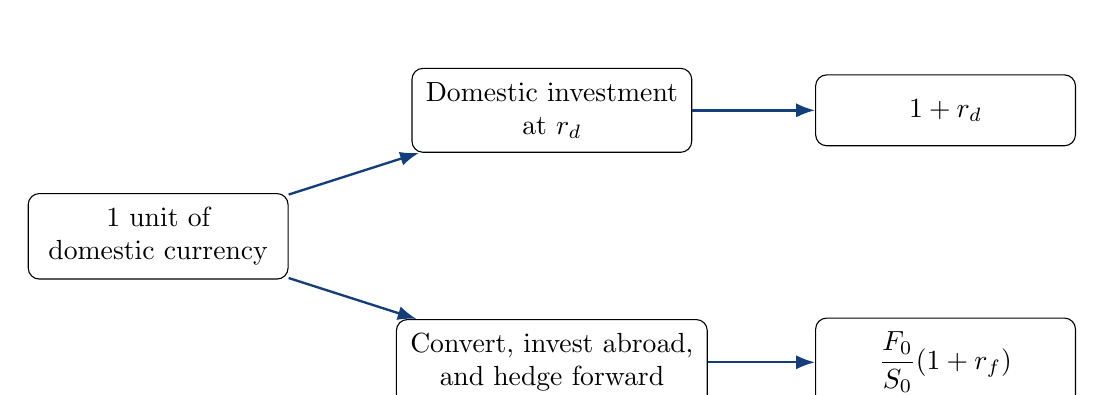
\begin{tikzpicture}[
> =Latex,
box/.style={
draw,
rounded corners,
align=center,
minimum width=3.3cm,
minimum height=0.9cm,
inner sep=5pt
},
flow/.style={-Latex, line width=0.85pt, FinanceBlue}
]
\node[box] (start) at (0,0)
{1 unit of\\domestic currency};

\node[box] (dom) at (5.0,1.6)
{Domestic investment\\at $r_d$};

\node[box] (for) at (5.0,-1.6)
{Convert, invest abroad,\\and hedge forward};

\node[box] (domend) at (10.0,1.6)
{$1+r_d$};

\node[box] (forend) at (10.0,-1.6)
{$\dfrac{F_0}{S_0}(1+r_f)$};

\draw[flow] (start) -- (dom);
\draw[flow] (start) -- (for);
\draw[flow] (dom) -- (domend);
\draw[flow] (for) -- (forend);

\end{tikzpicture}
\caption{Two covered investment paths underlying interest parity}
\label{fig:ch10-cip-paths}
\end{figure}

With continuously compounded rates over a horizon of $T$ years, the same relation can be written as

\begin{equation}
F_{0,T}
=S_0 e^{(r_d-r_f)T},
\label{eq:ch10-cip-continuous}
\end{equation}
where $r_d$ and $r_f$ are the corresponding domestic and foreign rates for the same maturity.

\begin{example}{A Forward Rate from Covered Interest Parity}{cip-forward-example}

Suppose the spot exchange rate is 7.20 domestic currency units per unit of foreign currency. The one-year domestic interest rate is 4\% and the comparable foreign rate is 2\%. Under the simplified CIP assumptions,

$$
F_0
=
7.20\times\frac{1.04}{1.02}
\approx
7.34.
$$

The foreign currency therefore trades at a forward premium under this quotation convention.

\end{example}

In practice, transaction costs, collateral terms, funding conditions, counterparty risk, regulation, and balance-sheet constraints can cause covered returns to differ from the simple parity benchmark. Such deviations indicate that the two funding paths are not economically identical once market frictions are taken into account.

\begin{tcolorbox}[
  enhanced,
  breakable,
  colback=white,
  colframe=FinanceBlue,
  boxrule=0.7pt,
  sharp corners,
  borderline west={2.2pt}{0pt}{FinanceBlue},
  title=\textbf{Financial Perspective: A Forward Rate Is Not a Forecast},
  coltitle=white,
  colbacktitle=FinanceBlue,
  fonttitle=\bfseries,
  before skip=1.2em,
  after skip=1.2em
]

An investor who purchases a foreign-currency asset
and sells the maturity proceeds forward locks in
a domestic-currency return. Without this hedge, the
realized return depends on the spot exchange rate
at maturity. The forward rate is therefore the price
of a contracted future exchange, whereas the expected
future spot rate reflects investors' expectations
and the compensation required for bearing exchange-rate
risk. The two need not coincide.

\end{tcolorbox}


\subsection{Uncovered Interest Parity and Currency Risk Premia}

Uncovered interest parity (UIP) compares expected
returns across currencies when exchange-rate risk
is not hedged. An investor in a foreign deposit
therefore remains exposed to the future spot
exchange rate. Unlike CIP, UIP does not eliminate
exchange-rate risk through a forward contract.
Its parity condition therefore concerns expected
returns rather than returns locked in by contractual
hedging.

Let $r_d$ and $r_f$ denote the domestic and foreign
interest rates over the same investment horizon.
The expected domestic-currency gross return on the
foreign deposit is

\begin{equation*}
(1+r_f)\frac{\mathrm{E}_0[S_1]}{S_0}.
\label{eq:ch10-uip-foreign-return}
\end{equation*}

A simple UIP benchmark equates this expected return
with the domestic gross return:

\begin{equation}
1+r_d
=
(1+r_f)\frac{\mathrm{E}_0[S_1]}{S_0}.
\label{eq:ch10-uip-exact}
\end{equation}

For moderate interest rates and exchange-rate changes,

\begin{equation}
\mathrm{E}_0\left[\frac{S_1-S_0}{S_0}\right]
\approx
r_d-r_f.
\label{eq:ch10-uip-approx}
\end{equation}

When the domestic interest rate exceeds the foreign
interest rate, the UIP benchmark implies an expected
depreciation of the domestic currency. 

When investors require compensation for bearing
currency risk, the expected domestic-currency return
on an unhedged foreign deposit may differ from the
return on a domestic deposit. Let $\rho$ denote the
difference between these two expected returns.

\begin{equation}
\rho
=
(1+r_f)\frac{\mathrm{E}_0[S_1]}{S_0}
-
(1+r_d).
\label{eq:ch10-currency-risk-premium}
\end{equation}

Since

\[
\frac{\mathrm{E}_0[S_1]}{S_0}
=
1+
\mathrm{E}_0\left[\frac{S_1-S_0}{S_0}\right],
\]
substitution gives

\begin{align}
\rho
={}&r_f-r_d
+\mathrm{E}_0\left[\frac{S_1-S_0}{S_0}\right]
+r_f\mathrm{E}_0\left[\frac{S_1-S_0}{S_0}\right].
\end{align}

For moderate interest rates and exchange-rate changes,
the product term can be neglected as a second-order
term. The resulting first-order approximation is

\begin{equation}
\rho
\approx
r_f-r_d
+
\mathrm{E}_0\left[\frac{S_1-S_0}{S_0}\right].
\label{eq:ch10-currency-risk-premium-approx}
\end{equation}

Rearranging gives

\begin{equation}
\mathrm{E}_0\left[\frac{S_1-S_0}{S_0}\right]
\approx
r_d-r_f+\rho.
\label{eq:ch10-uip-with-risk-premium}
\end{equation}

When $\rho=0$, the expected returns on the two
positions are equal, and the standard UIP benchmark
is recovered. When $\rho$ differs from zero, the
expected exchange-rate change also reflects the
compensation associated with bearing currency risk.


\section[Currency Exposure and Cross-Border Risk Allocation]{Currency Exposure and Cross-Border Risk\\ Allocation}

Currency exposure arises when cash flows, assets, or liabilities are denominated in currencies different from the currency in which their value is measured. Exchange-rate movements then redistribute value across contractual positions, while hedging and financing decisions determine how that risk is allocated among firms, investors, and financial intermediaries.

\subsection{Currency Denomination and Contractual Cash Flows}

Currency denomination specifies the unit in which
a contract promises payment. A dollar-denominated
bond promises dollar payments, while a
renminbi-denominated loan requires renminbi
repayment. Whether the denomination creates
exchange-rate exposure for a firm depends on its
valuation currency and the currency composition
of its revenues, assets, and other obligations.

For a firm with a foreign-currency liability,
the domestic-currency repayment cost varies with
the spot exchange rate. A depreciation of the
domestic currency increases the amount of domestic
currency required to meet the obligation. If the
firm's revenues are mainly denominated in domestic
currency, the foreign-currency debt creates a
currency mismatch. Foreign-currency revenues or
assets can offset part of this exposure and provide
a natural hedge.

Contract denomination does not capture all
exchange-rate exposure. A firm may reduce its
direct transaction exposure by choosing its
invoicing currency or hedging contractual cash
flows, while remaining exposed through changes
in revenues, input costs, competitive conditions,
and the value of foreign operations. The firm's
overall currency exposure therefore depends on
how exchange-rate movements affect its combined
operating and financial cash flows.


\subsection{Transaction Exposure}

Transaction exposure arises when a contracted foreign-currency cash flow is settled at a future date and its domestic-currency value remains sensitive to the exchange rate. It commonly arises from receivables, payables, and foreign-currency debt service.

Differentiating Equation~\eqref{eq:ch10-export-receivable-value}
with respect to $S_T$, holding the foreign-currency
receivable fixed, gives

\begin{equation}
\frac{\partial V_D,T}{\partial S_T}=V_{F,T}.
\label{eq:ch10-transaction-exposure-sensitivity}
\end{equation}

A rise in $S_T$ increases the domestic-currency value of a foreign-currency receivable and the domestic-currency cost of a foreign-currency payable. The economic effect therefore depends on the direction of the contractual cash flow.

Because transaction exposure is often associated with a specified amount and settlement date, it can frequently be matched with a forward or other hedging contract when the timing and amount are sufficiently predictable.

\begin{example}{Transaction Exposure on an Export Receivable}
{transaction-exposure-exporter}

A Chinese exporter will receive USD~5 million in
90 days. If the spot exchange rate at settlement
is RMB~7.00 per dollar, the receipt converts to
RMB~35.0 million. If the exchange rate instead
reaches RMB~7.40 per dollar, the receipt converts
to RMB~37.0 million.

The increase of RMB~0.40 per dollar raises the
domestic-currency value of the receivable by
RMB~2.0 million:

\[
\Delta V_{D,T}
=
V_{F,T}\Delta S_T
=
5\times 0.40
=
\text{RMB }2.0\text{ million}.
\]

The example illustrates the exchange-rate
sensitivity of a fixed foreign-currency receivable:
a higher $S_T$ increases its domestic-currency
value, while a lower $S_T$ reduces it.

\end{example}


\subsection{Translation Exposure}

Translation exposure arises when foreign-currency financial statements or balance-sheet positions are converted into a firm's reporting currency. It is particularly relevant for multinational firms with foreign operations.

Suppose a parent company reports in domestic currency while a foreign subsidiary keeps its accounts in another currency. Changes in the exchange rate can alter the reported domestic-currency value of the subsidiary's assets, liabilities, revenues, and expenses even when no corresponding cash flow occurs between the subsidiary and the parent.

Translation exposure therefore differs from transaction exposure. Transaction exposure arises from contracted foreign-currency cash flows that will be settled, whereas translation exposure arises from converting accounting amounts into the reporting currency. A translation loss does not by itself create an immediate cash payment.

Translation effects can nevertheless influence reported equity, earnings, leverage, and other financial measures. Their significance depends on the firm's balance-sheet structure, reporting framework, and any contractual or regulatory provisions linked to reported accounting values.

Accounting treatment determines where translation effects appear in the financial statements. The specific treatment varies across accounting frameworks, so exposure analysis should distinguish the underlying foreign-currency position from its accounting representation.

\subsection{Economic Exposure}

Economic exposure, sometimes called operating exposure, is the sensitivity of the present value of future operating cash flows to exchange-rate changes. It extends beyond contracted foreign-currency receivables and payables.

A firm can face economic exposure even when its sales and contracts are denominated in domestic currency. Exchange-rate movements can alter the relative prices of domestic and foreign products, the cost of imported inputs, and the competitive position of the firm. These changes can affect sales volumes, margins, and future operating cash flows.

The direction and magnitude of economic exposure depend on the structure of the firm's revenues and costs. A domestic-currency depreciation may increase the value of foreign revenues, but imported inputs, foreign-currency debt, or competitive responses can offset part of that effect. Economic exposure therefore cannot always be inferred from the currency denomination of existing contracts.


\begin{table}[htbp]
\centering
\caption{Three forms of currency exposure}
\label{tab:ch10-currency-exposure-types}

\begin{tabularx}{\textwidth}{@{}p{3.1cm}X X@{}}
\toprule
\textbf{Exposure}
& \textbf{Source}
& \textbf{Illustrative effect} \\
\midrule

Transaction exposure
& Contracted foreign-currency cash flows
& Domestic value changes before settlement \\

Translation exposure
& Conversion of foreign operations into the reporting currency
& Reported accounting values change with the translation rate \\

Economic exposure
& Exchange-rate effects on prices, costs, demand, and competition
& Present value of future operating cash flows changes \\

\bottomrule
\end{tabularx}
\end{table}

Economic exposure can also change as firms adjust sourcing, production, pricing, and financing. Short-run exposure based on current operating arrangements may therefore differ from longer-run exposure after firms respond to exchange-rate changes. The main sources and effects of transaction, translation, and economic exposure are summarized in Table~\ref{tab:ch10-currency-exposure-types}.
The three forms of exposure can overlap. A foreign operation may create translation and economic exposure, while a specific foreign-currency contract can create transaction exposure within the firm's broad


\subsection{Hedging Logic and the Allocation of Exchange-Rate Risk}

Hedging changes the sensitivity of a position to exchange-rate movements. The objective is generally to offset an identified exposure rather than to predict the direction of the exchange rate.

Consider an exporter with a foreign-currency
receivable of $V_{F,T}$ due at date $T$. If the
exporter sells a fraction $h$ of the receivable
forward at the rate $F_{0,T}$, the settlement
gain or loss on the forward position relative
to conversion at the spot rate is

\begin{equation}
hV_{F,T}\times(F_{0,T}-S_T).
\label{eq:ch10-export-forward-payoff}
\end{equation}

Combining the forward payoff with the conversion
of the remaining unhedged receivable gives the
domestic-currency value of the hedged position:

\begin{equation}
V_{D,T}^{H}
=
V_{F,T}\left[(1-h)S_T+hF_{0,T}\right].
\label{eq:ch10-partial-forward-hedge}
\end{equation}

When $h=0$, the receivable remains fully exposed
to the future spot rate. When $h=1$ and the
forward contract matches the amount and maturity
of the receivable,

\begin{equation}
V_{D,T}^{H}=F_{0,T}V_{F,T}.
\label{eq:ch10-full-forward-hedge}
\end{equation}

The hedge therefore replaces part or all of the
uncertain future conversion rate with a rate
fixed in advance. It reduces the exchange-rate
sensitivity of the specified cash flow, while
other risks associated with the underlying
transaction remain.

\begin{example}{A Full and Partial Forward Hedge}{forward-hedge-example}

A firm will receive USD~4 million in six months, and the six-month forward rate is RMB~7.25 per dollar. A full forward hedge locks in

$$
4\times 7.25)=29.0
$$
million RMB.

If the firm instead hedges 60\% of the receivable, the domestic-currency value becomes

$$
4\times\left[0.4S_T+0.6\times 7.25\right].
$$

At a future spot rate of RMB~7.00 per dollar, the receipt is RMB~28.6 million; at RMB~7.50 per dollar, it is RMB~29.4 million. Partial hedging reduces, but does not eliminate, sensitivity to the future spot rate.

\end{example}

The same logic applies to other hedging instruments. Futures provide standardized contracts, options alter the distribution of exchange-rate outcomes, and currency swaps can transform streams of cash flows across currencies. Firms may also create natural hedges by aligning the currencies of revenues, costs, assets, and liabilities. The relevant question in each case is how the hedge payoff offsets the underlying exposure.

The hedge ratio need not equal one. If the amount or timing of the underlying cash flow is uncertain, a full hedge can leave the firm with a new currency position when the realized exposure differs from the amount hedged. Derivative hedges can also create collateral or liquidity requirements before the underlying cash flow is received.

Exchange-rate risk can also be allocated through the commercial or financing contract itself. An exporter that invoices in domestic currency shifts more transaction exposure to the foreign buyer; borrowing in the currency of future revenues can place part of the exposure on the liability side. Contract denomination, operating choices, and financial hedging therefore provide alternative ways of distributing exchange-rate risk across participants.

\begin{tcolorbox}[
enhanced,
breakable,
colback=white,
colframe=FinanceBlue,
boxrule=0.7pt,
sharp corners,
borderline west={2.2pt}{0pt}{FinanceBlue},
title=\textbf{Financial Perspective: Hedge the Exposure, Not the Forecast},
coltitle=white,
colbacktitle=FinanceBlue,
fonttitle=\bfseries,
before skip=1.2em,
after skip=1.2em
]

A hedge is most effective when the amount, currency, and timing of the hedging position correspond to the underlying exposure. The purpose is to alter the distribution of cash-flow outcomes, not to establish a view about the future exchange rate.

\end{tcolorbox}


%========================================================% Summary
%========================================================

\TailModule{summary}{Summary}

Foreign exchange markets connect claims denominated in different currencies. Trade, investment, and cross-border funding create currency-conversion needs when cash flows and valuation currencies differ. Dealers and electronic venues redistribute these flows across a decentralized market, while trading and settlement arrangements influence liquidity and execution.

Exchange-rate interpretation begins with the quote convention. In this chapter, the exchange rate is domestic currency per unit of foreign currency, so an increase represents domestic-currency depreciation. Real exchange rates incorporate relative price levels, while effective exchange rates summarize movements against multiple trading partners. Exchange-rate regimes differ in how market pressure is absorbed between exchange-rate adjustment and policy action.

Parity relations provide benchmarks under stated assumptions. The law of one price and purchasing power parity link goods prices to exchange rates through goods-market arbitrage. Covered interest parity links spot rates, forward rates, and interest rates through covered return comparisons, while uncovered interest parity links interest differentials to expected exchange-rate changes under assumptions about expected returns and currency risk premia. The forward rate therefore need not equal the expected future spot rate.

Currency exposure arises through contracts, accounting positions, operating cash flows, and financing. Transaction exposure concerns contracted foreign-currency cash flows, translation exposure concerns the conversion of foreign operations into the reporting currency, and economic exposure concerns the sensitivity of future operating cash flows to exchange-rate movements. Financial hedges and natural hedges can reduce or redistribute these exposures when their amount, timing, and currency correspond sufficiently closely to the underlying position.


%========================================================
% Key Terms
%========================================================

\TailModule{keyterms}{Key Terms}

Foreign exchange market; spot exchange rate; direct quote;  bid--ask spread; cross rate; triangular arbitrage; market liquidity; nominal exchange rate; real exchange rate; nominal effective exchange rate; real effective exchange rate; fixed exchange-rate regime; floating exchange-rate regime; managed exchange-rate regime; foreign exchange intervention; law of one price; purchasing power parity; covered interest parity; forward exchange rate; uncovered interest parity; currency risk premium; currency denomination; transaction exposure; translation exposure; economic exposure; forward hedge; hedge ratio.

%========================================================
% Financial AI Lab
%========================================================

\TailModule{aiprompt}{Financial AI Lab}

\textbf{Lab: Audit an FX Quote, a Parity Calculation, and a Hedge}

Ask an AI system to analyze a one-year cross-currency investment using a spot exchange rate, domestic and foreign interest rates, and a one-year forward rate. Require it to state the exchange-rate quote convention before performing any calculation.

Audit the analysis in four stages.

\begin{enumerate}

\item \textbf{Check the quote direction.} Identify the currencies in the numerator and denominator and verify that appreciation and depreciation are interpreted consistently with the quote.

\item \textbf{Check covered interest parity.} Place the two interest rates on the same maturity and compounding basis. Calculate the forward rate implied by covered interest parity and compare it with the supplied forward rate. Before treating any difference as an arbitrage opportunity, consider transaction costs, funding and collateral conditions, and other relevant market frictions.

\item \textbf{Separate pricing from forecasting.} Ask the AI to interpret the forward rate as a possible forecast of the future spot rate. Check whether it distinguishes the covered pricing relation from expectations about future exchange rates and currency risk premia.

\item \textbf{Audit the hedge.} Give the AI a foreign-currency receivable and ask it to calculate the domestic-currency cash flow under no hedge, a partial forward hedge, and a full forward hedge. Verify the direction of the forward position and test the results under both appreciation and depreciation of the domestic currency.

\end{enumerate}


%========================================================
% Discussion Questions
%========================================================

\TailModule{questions}{Discussion Questions}

\begin{enumerate}

\item Why can a foreign investment earn a positive return in its local currency but generate a negative return for a domestic investor after currency conversion?

\item Why can a country with a floating exchange rate still intervene in the foreign exchange market? How does such intervention differ from maintaining a fixed parity?

\item Why does covered interest parity provide a stronger arbitrage benchmark than uncovered interest parity?

\item A firm's export contracts are denominated entirely in its domestic currency. Why can the firm still have economic exposure to exchange-rate movements?

\end{enumerate}


%========================================================
% Applied Problems
%========================================================

\TailModule{appprobs}{Applied Problems}

\begin{enumerate}

\item \textbf{Quotes, appreciation, and cross rates.}

The spot exchange rate is RMB~7.24 per U.S. dollar and USD~1.08 per euro.

\begin{enumerate}

\item Calculate the reciprocal USD/RMB quote.

\item If RMB/USD rises to 7.38, has the renminbi appreciated or depreciated against the dollar under the quotation convention used in this chapter?

\item Calculate the implied RMB/EUR cross rate using the original quotations.

\item Explain what trading pressure could arise if the directly quoted RMB/EUR rate differed from the implied cross rate by more than transaction costs and other execution frictions.

\end{enumerate}

\item \textbf{Nominal and real exchange rates.}

The domestic currency depreciates by 6\% over one year under the quotation convention used in this chapter. Domestic inflation is 4\% and foreign inflation is 2\%.

\begin{enumerate}

\item Using the approximation in Equation~(\ref{eq:ch10-real-exchange-rate-change}), estimate the percentage change in the real exchange rate.

\item Recalculate the real exchange-rate change if domestic inflation is 9\%, holding the other values unchanged.

\item Explain why nominal depreciation need not imply real depreciation.

\end{enumerate}

\item \textbf{Covered interest parity.}

The spot exchange rate is 7.20 domestic currency units per unit of foreign currency. The one-year domestic interest rate is 4.5\% and the comparable foreign rate is 2.0\%.

\begin{enumerate}

\item Calculate the one-year forward rate implied by covered interest parity.

\item Calculate the forward premium as a percentage of the spot rate.

\item Suppose the observed forward rate is 7.30. What additional information would be needed before concluding that a tradable arbitrage opportunity exists?

\item Explain why the CIP-implied forward rate is not necessarily a forecast of the future spot rate.

\end{enumerate}

\item \textbf{Uncovered returns and currency risk premia.}

The domestic one-year interest rate is 5\% and the foreign rate is 3\%. The domestic currency is expected to depreciate by 4\% over the year.

\begin{enumerate}

\item Using the first-order approximation in Equation~\ref{eq:ch10-currency-risk-premium}, calculate the expected excess return on the unhedged foreign deposit relative to the domestic deposit.

\item Does the zero-risk-premium UIP benchmark hold under these expectations?

\item What expected exchange-rate change would be consistent with zero-risk-premium UIP?

\item Explain how a time-varying currency risk premium affects the interpretation of the interest differential.

\end{enumerate}

\item \textbf{Currency exposure and hedging.}

A domestic exporter will receive USD~8 million in six months. The six-month forward rate is RMB~7.18 per dollar, and the firm chooses a hedge ratio of 75\%.

\begin{enumerate}

\item Calculate the domestic-currency value of the hedged receipt if the future spot rate is RMB~6.95 per dollar.

\item Recalculate the value if the future spot rate is RMB~7.45 per dollar.

\item Using the same two exchange-rate outcomes, compare the range of hedged receipts with the range under no hedge.

\item Calculate the domestic-currency value locked in under a full hedge.

\item Identify one risk that remains even under a full currency hedge.

\end{enumerate}

\end{enumerate}


%========================================================
% Data Application
%========================================================

\TailModule{dataapp}{Data Application}

\textbf{Bilateral, Nominal Effective, and Real Effective Exchange Rates of the Renminbi}

Obtain a monthly RMB exchange rate against the U.S. dollar from an authoritative Chinese source and nominal and real effective exchange-rate indexes for China from an authoritative source with documented methodology.

Use a sample of at least five years. Convert the series to a common starting value of 100 where appropriate, and plot the bilateral RMB/USD rate, the nominal effective exchange-rate index, and the real effective exchange-rate index. State the quotation convention for the bilateral rate and the direction in which an increase in each index is defined.

Identify at least two periods in which the bilateral exchange rate and the effective-rate indexes moved differently. Explain how movements in other trading-partner currencies could contribute to the divergence. Then compare the nominal and real effective indexes and relate their differences to relative price or cost changes.

Interpret the effective exchange-rate measures with care. They summarize currency movements across trading partners but do not provide a complete measure of international competitiveness. Discuss at least two additional factors that may affect the broader economic interpretation.

Report the sample period, frequency, index definitions, source institutions, and any transformations applied to the data.


%========================================================
% Further Reading
%========================================================

\TailModule{furtherread}{Further Reading}

\begin{itemize}

\item Dornbusch, R"udiger (1976),
``Expectations and Exchange Rate Dynamics,''
\emph{Journal of Political Economy}, 84(6), 1161--1176.

\item Meese, Richard A., and Kenneth Rogoff (1983),
``Empirical Exchange Rate Models of the Seventies: Do They Fit Out of Sample?''
\emph{Journal of International Economics}, 14(1--2), 3--24.

\item Fama, Eugene F. (1984),
``Forward and Spot Exchange Rates,''
\emph{Journal of Monetary Economics}, 14(3), 319--338.

\item Obstfeld, Maurice, and Kenneth Rogoff (1995),
``The Mirage of Fixed Exchange Rates,''
\emph{Journal of Economic Perspectives}, 9(4), 73--96.

\item Du, Wenxin, Alexander Tepper, and Adrien Verdelhan (2018),
``Deviations from Covered Interest Rate Parity,''
\emph{The Journal of Finance}, 73(3), 915--957.

\end{itemize}


\ChapterTail{summary,keyterms,aiprompt,questions,appprobs,dataapp,furtherread}

\chapter{Derivatives Markets and Contingent Claims}
\label{chap:Derivatives_Markets_and_Contingent_Claims}

\begin{openingcase}{How Do Derivatives Markets Organize Risk Transfer?}

A manufacturer with operations in several countries uses foreign-exchange forwards, interest-rate swaps, and commodity options to manage different financial exposures. Some contracts are standardized and traded on organized exchanges, where central clearing, margining, and daily settlement support market-wide trading. Others are negotiated bilaterally with dealers to match the firm's currency, maturity, notional amount, and payment dates more closely.

The firm therefore uses more than one type of derivatives market. The choice affects contract flexibility, price transparency, liquidity, counterparty exposure, collateral requirements, and the way positions are valued and settled. A customized contract may provide a closer hedge, while a standardized contract may be easier to trade or clear.

The underlying business exposures remain with the firm. What changes is the market architecture through which selected risks are transferred, priced, and managed.

\end{openingcase}



\begin{tcolorbox}[
  enhanced,
  colback=FinanceBlue!6,
  colframe=FinanceBlue,
  boxrule=0.6pt,
  sharp corners,
  left=8pt,
  right=8pt,
  top=7pt,
  bottom=7pt,
  before skip=1em,
  after skip=1.6em,
  title=\textbf{Core Questions},
  coltitle=white,
  colbacktitle=FinanceBlue,
  fonttitle=\bfseries,
  attach boxed title to top left={xshift=6pt,yshift=-2mm},
  boxed title style={
    boxrule=0pt,
    sharp corners,
    left=5pt,
    right=5pt,
    top=2pt,
    bottom=2pt
  }
]
\begin{enumerate}[
  leftmargin=*,
  label=\textcolor{FinanceBlue}{\textbf{\arabic*.}},
  itemsep=0.55em,
  topsep=0.2em
]


\item How do derivatives use state-contingent claims to unbundle and reallocate financial exposures?

\item How do no-arbitrage and replication connect derivative prices to the prices of other traded claims?

\item How do exchange trading, bilateral contracting, collateral, netting, and central clearing affect counterparty risk and the allocation of risk in derivative markets?


\end{enumerate}
\end{tcolorbox}

\section[Why Derivatives Exist: Contingent Claims and Risk Allocation]{Why Derivatives Exist:\\ Contingent Claims and Risk Allocation}

A derivative is a financial contract whose payoff depends on the value of an underlying asset, rate, index, event, or other specified condition. Its economic role is not confined to speculation. Derivatives allow participants to separate exposures that are bundled together in ordinary business and financial positions and to transfer selected parts of those exposures to other market participants.

\subsection{State-Contingent Payoffs}

A contingent claim is a financial claim whose payoff
depends on the future state of the world. Let the
possible states at date $T$ be indexed by
$s=1,\ldots,S$. The payoff of a claim in state $s$
is denoted by $X_T(s)$.

A state represents the future conditions relevant
to the contractual payoff. These conditions may
include the price of an underlying asset, an interest
rate, an exchange rate, a commodity price, or the
occurrence of a specified credit event. A contingent
claim therefore specifies how a contractual payment
varies across possible future states.

A forward contract illustrates a linear
state-contingent payoff. It specifies the purchase
and sale of an underlying asset at a future date $T$
for a delivery price $K$ agreed upon at inception.
The party obligated to purchase the underlying asset
holds the long position, while the party obligated
to deliver it holds the short position.

At maturity, the payoff per unit of the underlying
asset to the long forward position is

\begin{equation}
X_T^{\mathrm{long}}
=
S_T-K.
\label{eq:ch11-forward-long-payoff}
\end{equation}

The short forward position has the opposite payoff:

\begin{equation}
X_T^{\mathrm{short}}
=
K-S_T
=
-X_T^{\mathrm{long}}.
\label{eq:ch11-forward-short-payoff}
\end{equation}

Here, $S_T$ denotes the market price of the underlying
asset at maturity. The two positions have equal and
opposite payoffs before transaction costs and
counterparty losses.

Options also create state-contingent claims, but
their holders possess exercise rights rather than
an unconditional obligation to transact. Their
nonlinear payoff structures are examined in
later chapters.

The same state-contingent perspective applies more
broadly to debt, equity, insurance contracts, and
guarantees. These claims distribute payments
differently across future states, reflecting
differences in contractual priority, risk allocation,
and the conditions governing payment.

\subsection{Exposure Decomposition and Risk Unbundling}

Financial and operating positions often contain several sources of risk at the same time, and these exposures may interact. For example, the cash flow of an importing firm may be affected by both commodity prices and exchange rates, while joint movements in the two variables can amplify or partially offset changes in the firm's domestic-currency input costs. The risk of a position therefore depends not only on its individual exposures, but also on how those exposures move together.

Exposure decomposition separates an overall position into economically distinct sources of risk and identifies how each source affects the position's cash flows or value. This makes it possible to distinguish exposures that may be retained from those that may be reduced or otherwise modified.

Once distinct exposures have been identified, derivatives can be used to modify them separately. A derivative linked to a particular price, rate, index, or event creates a payoff that responds to that source of risk without requiring the underlying business activity or asset position to be changed. In this way, an exposure embedded in a broader position can be unbundled and modified separately from the other components of the position.

To illustrate risk unbundling, suppose an existing position has value $V_T$ at date $T$ and is exposed to several risk factors. A derivative linked to one of these factors has payoff $X_T$. The combined position is

\begin{equation}
V_T^{D}=V_T+X_T.
\label{eq:ch11-combined-derivative-position}
\end{equation}

Because $X_T$ responds to a selected risk factor, that component of the original exposure can be modified separately from the others. If the derivative payoff offsets part of the cash-flow variation associated with that factor, the combined position becomes less sensitive to it. If the payoff reinforces the existing exposure, sensitivity to the factor can increase.

Hedging is one application of this mechanism. By taking a derivative position with an offsetting payoff, a participant can reduce a selected exposure while leaving other components of the original position largely unchanged.

\subsection{Risk Sharing and Market Completeness}

Risk sharing becomes more flexible when market participants can trade claims with different state-contingent payoffs. A firm seeking more stable cash flows may transfer part of an exposure to another participant willing to bear it in exchange for compensation or because the exposure fits the participant's other positions. Derivatives facilitate such transfers by creating contractual payoffs tied to particular future states.

The extent of risk sharing depends on the range of payoffs that can be constructed from traded claims. Consider a simple economy with two future states, denoted by $u$ and $d$. Suppose two traded securities have payoff vectors

\begin{equation}
\mathbf{x}_1=
\begin{bmatrix}
x_{1u}\\
x_{1d}                                                      
\end{bmatrix},
\qquad
\mathbf{x}_2=
\begin{bmatrix}
x_{2u}\\
x_{2d}
\end{bmatrix}.
\label{eq:ch11-two-security-payoffs}
\end{equation}

A portfolio with holdings $a$ and $b$ in the two
securities produces the following state-contingent
payoff vector:

\begin{equation}
\mathbf{x}_p
=
a\mathbf{x}_1+b\mathbf{x}_2
=
\begin{bmatrix}
ax_{1u}+bx_{2u}\\
ax_{1d}+bx_{2d}
\end{bmatrix},
\label{eq:ch11-spanning-portfolio}
\end{equation}

Positive values of $a$ and $b$ represent long
positions in the respective securities, whereas
negative values represent short positions.

If the two payoff vectors are linearly independent,
they span the two-dimensional state-payoff space.
Consequently, suitable portfolio holdings can
generate any payoff vector across the two states.
A market in which every relevant state-contingent
payoff can be constructed from available traded
claims is called a \emph{complete market}.

If the available claims cannot generate all relevant state-contingent payoffs, the market is incomplete. Some desired patterns of cash flows cannot then be constructed exactly, and participants may continue to bear residual exposures after trading the available instruments.

In actual markets, transaction costs, trading restrictions, nontradable risks, model uncertainty, and a limited range of contracts may prevent some desired state-contingent payoffs from being constructed.

Derivatives can expand the range of available state-contingent payoffs by introducing claims linked to risks not fully represented by existing securities. This can increase the range of risks that can be transferred and shared across market participants. Derivatives do not create additional economic resources; they redistribute future cash flows and risks across states and participants.

\subsection{Financial Innovation and New Claims}

In an incomplete market, some desired state-contingent payoffs cannot be constructed from existing claims. Financial innovation can partly address this gap by creating new derivatives linked to particular prices, rates, indices, events, or maturities. These new claims can expand the range of exposures that can be transferred or hedged.

New claims can be designed by changing either the reference basis or the payoff rule. A contract may be linked to a new commodity index, volatility measure, or credit event. Its payoff structure may also be redesigned through caps, floors, barrier features, or path-dependent conditions. By altering what the contract is linked to or how its payoff is determined, innovation changes the state-contingent cash flows available to market participants.

A closer match, however, does not eliminate all risk. A customized claim may reduce basis risk by tracking the underlying exposure more closely, but it may trade less actively or create greater dependence on a particular counterparty. A standardized claim may offer greater liquidity while providing a less exact match to the exposure being managed. Financial innovation therefore changes not only which risks can be transferred, but also the form of the residual risks that remain.

\section{No-Arbitrage and Replication}

Derivative markets rely on two related mechanisms \cite{BlackScholes1973,Merton1973,HarrisonKreps1979}
to maintain pricing consistency. No-arbitrage
restricts the relative prices of claims according
to their state-contingent payoffs, while replication
uses portfolios of traded securities to construct
equivalent payoffs. Together, these mechanisms
provide the basis for valuing derivative contracts.

\subsection{Arbitrage Opportunities and Price Consistency}

The law of one price requires derivative positions
with identical state-contingent cash flows to have
the same current price. A meaningful comparison
requires matching underlying references, notional
amounts, maturities, payment dates, settlement
currencies, and other payoff-determining contractual
terms. Differences in these features may produce
different cash flows and do not necessarily indicate
inconsistent pricing.

An arbitrage opportunity can take two forms.
The first involves a zero initial net investment
and nonnegative future payoffs in every state,
with a strictly positive payoff in at least one
state. The second generates a positive initial
cash inflow without creating any future net payment
obligation. Both forms allow a trader to obtain
a gain without bearing an offsetting future loss.

\paragraph{First Type: Arbitrage from Payoff Dominance.}

A first form of arbitrage arises when two
derivative claims have the same current price,
but one provides at least as much as the other
in every future state and strictly more in at
least one state. Suppose

\begin{equation}
P_A=P_B,
\qquad
X_A(s)\geq X_B(s), \quad \forall s,
\label{eq:ch11-payoff-dominance}
\end{equation}
with strict inequality in at least one possible
state. An investor can purchase $A$ and sell $B$
short. The strategy requires zero initial net
investment:

\begin{equation}
\Pi_0=P_B-P_A=0.
\end{equation}

Its future net payoff satisfies

\begin{equation}
\Pi_T(s)=X_A(s)-X_B(s)\geq 0,
\qquad \forall s,
\end{equation}
with a strictly positive payoff in at least
one state. This strategy generates nonnegative
future payoffs without requiring an initial
investment and constitutes an arbitrage
opportunity.

Under the no-arbitrage condition, a claim that
provides at least as much as another in every
relevant state and strictly more in at least one
state must have a strictly higher current price,
provided the corresponding trading positions
can be established.

\paragraph{Second Type: Arbitrage between Equivalent-Payoff Claims.}

Consider two traded derivative positions, $A$ and
$B$, with identical contractual cash flows at the
same dates in every relevant future state. Let
$P_A$ and $P_B$ denote their current prices, and
let $X_A(s)$ and $X_B(s)$ denote their respective
payoffs in state $s$. Their payoff equivalence
requires

\begin{equation}
X_A(s)=X_B(s),
\qquad \forall s.
\label{eq:ch11-equivalent-derivative-payoffs}
\end{equation}

If $P_A<P_B$, an investor can purchase $A$ and
sell $B$ short. The initial net cash inflow is

\begin{equation}
\Pi_0=P_B-P_A>0,
\end{equation}

while the future net payoff is

\begin{equation}
\Pi_T(s)=X_A(s)-X_B(s)=0,
\qquad \forall s.
\end{equation}

The strategy generates a positive initial cash
inflow without creating a future net payment
obligation. If $P_A>P_B$, reversing the two
positions produces the corresponding opportunity.
Under the no-arbitrage condition, equivalent
derivative positions must therefore have the
same current price.

\begin{example}{Arbitrage from Payoff Dominance}
{ch11-payoff-dominance-arbitrage}

Consider two derivative claims with the same
maturity and settlement currency. Their current
prices and payoffs across two possible states are:

\begin{center}
\begin{tabular}{lcc}
\toprule
\textbf{Position}
& \textbf{State 1}
& \textbf{State 2} \\
\midrule
Claim A (price 9) & 12 & 20 \\
Claim B (price 9) & 10 & 20 \\
\midrule
Long A, short B & 2 & 0 \\
\bottomrule
\end{tabular}
\end{center}

Purchasing A and selling B short requires no
initial net investment. The resulting position
generates a positive payoff in state 1 and zero
payoff in state 2. The equal current prices are
therefore inconsistent with the no-arbitrage
condition. In an arbitrage-free market, claim A
must have a higher current price than claim B.

\end{example}

In actual markets, theoretical arbitrage opportunities
may not be fully exploitable. Transaction costs,
bid--ask spreads, short-sale restrictions, funding
and collateral requirements, and counterparty risk
affect the feasibility and net returns of arbitrage
strategies. 

Price consistency may also be assessed against
portfolios of traded securities when no single
traded claim provides an equivalent payoff.


\subsection{Replication and Synthetic Positions}

Replication concerns the construction of a portfolio
whose state-contingent payoffs match those of a target
financial claim. A portfolio that reproduces the
payoffs of another claim is called a
\emph{synthetic position}. When replication is exact,
the two positions have identical future cash flows
and must have the same current value under
no-arbitrage conditions.

Consider a market with $J$ traded securities and
$S$ possible future states. Let $X_j(s)$ denote the
payoff of security $j$ in state $s$, and let $P_j$
denote its current price. A portfolio holding
$\theta_j$ units of each security generates the
payoff

\begin{equation}
X_p(s)
=
\sum_{j=1}^{J}\theta_j X_j(s),
\qquad s=1,\ldots,S.
\label{eq:ch11-replicating-portfolio-payoff}
\end{equation}

Suppose a target claim has payoff $X(s)$ in state
$s$. Replication requires the portfolio to satisfy

\begin{equation}
\sum_{j=1}^{J}\theta_j X_j(s)
=
X(s),
\qquad s=1,\ldots,S.
\label{eq:ch11-replication-conditions}
\end{equation}

In matrix notation, this condition is

\begin{equation}
\mathbf{X}\boldsymbol{\theta}
=
\mathbf{x},
\label{eq:ch11-replication-matrix}
\end{equation}
where $\mathbf{X}$ is the matrix of traded-security
payoffs, $\boldsymbol{\theta}$ is the vector of
portfolio holdings, and $\mathbf{x}$ is the target
claim's payoff vector.

The current cost of the replicating portfolio is

\begin{equation}
P_p
=
\sum_{j=1}^{J}\theta_j P_j.
\label{eq:ch11-replicating-portfolio-cost}
\end{equation}

If the portfolio exactly reproduces the target
claim's contractual cash flows, no-arbitrage
requires the claim's current price $P_X$ to equal the
replication cost:

\begin{equation}
P_X=P_p
=
\sum_{j=1}^{J}\theta_j P_j.
\label{eq:ch11-replication-pricing}
\end{equation}

If the target claim trades above the replication
cost, an investor can purchase the replicating
portfolio and sell the claim. If it trades below
the replication cost, the reverse position applies.
In either case, the difference in current prices
can be captured while the future payoffs offset
in every state.

\begin{example}{Replicating a Contingent Protection Claim}
{ch11-contingent-protection-replication}

Consider an economy with three possible future
states: expansion, slowdown, and severe downturn.
Three securities are traded in the market. Their
current prices are RMB~44.20, RMB~65.00, and
RMB~48.00, respectively. Their payoffs per unit
across the three states are shown below.

\begin{center}
\begin{tabular}{@{}lccc@{}}
\toprule
\textbf{State}
& \textbf{Security 1}
& \textbf{Security 2}
& \makecell{\textbf{Risk-free}\\\textbf{security}} \\
\midrule
Expansion       & 100 & 20  & 50 \\
Slowdown        & 50  & 50  & 50 \\
Severe downturn & 20  & 100 & 50 \\
\bottomrule
\end{tabular}
\end{center}

Suppose a business-interruption protection claim
pays RMB~0 in an expansion, RMB~50 in a slowdown,
and RMB~100 in a severe downturn. Its payoff vector
is

\[
\mathbf{x}
=
\begin{bmatrix}
0\\
50\\
100
\end{bmatrix}.
\]

A portfolio of the three traded securities can
reproduce this payoff. Let $\theta_1$, $\theta_2$,
and $\theta_3$ denote the respective holdings.
The replication conditions are

\begin{align*}
100\theta_1+20\theta_2+50\theta_3&=0,\\
50\theta_1+50\theta_2+50\theta_3&=50,\\
20\theta_1+100\theta_2+50\theta_3&=100.
\end{align*}

Solving these equations gives

\[
\theta_1=-0.625,\qquad
\theta_2=0.625,\qquad
\theta_3=1.
\]

The replicating portfolio therefore consists of
a short position in 0.625 units of Security 1,
a long position in 0.625 units of Security 2,
and a long position in one unit of the risk-free
security.

Its current cost is

\begin{align*}
P_p
&=-0.625(44.20)+0.625(65)+48\\
&=61.
\end{align*}

The portfolio reproduces the protection claim's
payoffs in all three states. Under the stated
no-arbitrage conditions, the current value of
the claim is therefore RMB~61.

\end{example}

Replication is distinct from hedging in a broader
sense. A hedge may reduce the sensitivity of an
existing position to selected risk factors without
eliminating all state-dependent differences.
Exact replication, by contrast, requires the
portfolio to match the target claim's payoff in
every relevant state.

\section{Derivative Market Architecture and Risk Infrastructure}

Derivative market architecture determines how trading relationships are formed, how exposures are offset, and how counterparty risk is redistributed. Standardization and centralized trading can concentrate liquidity and improve price discovery, while collateral, netting, and clearing limit bilateral exposure and reorganize the transmission of losses across market participants.

\subsection{Trading Venues: Exchange-Traded and Over-the-Counter Markets}

Derivatives can trade on organized exchanges or through over-the-counter (OTC) arrangements. Exchange-traded derivatives generally use standardized contract terms, including contract size, maturity, settlement terms, and other specifications. Standardization allows many participants to trade contracts with common terms and makes positions more interchangeable.

OTC derivatives are negotiated between counterparties, often under standardized legal documentation while allowing economic terms to be tailored. Notional amount, maturity, reference variable, and settlement provisions can therefore be adjusted to match a particular exposure more closely. Greater customization, however, can make contracts less interchangeable and positions more difficult to transfer.

The distinction is not absolute. Some OTC derivatives use highly standardized terms and may be centrally cleared, while electronic trading platforms have reduced the traditional separation between exchange and dealer-based execution. Trading venue, contract design, and clearing arrangement are therefore related but distinct dimensions of derivative-market organization.

Major derivative exchanges provide concrete examples of how standardized contracts are organized within formal trading venues. Table~\ref{tab:ch11-major-derivative-exchanges} presents selected examples from China and major international markets.

\begin{table}[H]
\centering
\caption{Examples of Major Exchange-Traded Derivative Markets}
\label{tab:ch11-major-derivative-exchanges}

\begin{tabularx}{\textwidth}{p{3.8cm} p{3.2cm} X}
\toprule
\textbf{Exchange} &
\textbf{Market Focus} &
\textbf{Representative Derivatives} \\
\midrule

China Financial Futures Exchange (CFFEX) &
Financial derivatives &
Equity-index futures and options; government-bond futures \\

Shanghai Futures Exchange (SHFE) &
Commodity derivatives &
Metals, energy, and other commodity futures and options \\

Dalian Commodity Exchange (DCE) &
Commodity derivatives &
Agricultural, industrial, and chemical futures and options \\

Zhengzhou Commodity Exchange (ZCE) &
Commodity derivatives &
Agricultural, energy, and industrial futures and options \\

Guangzhou Futures Exchange (GFEX) &
Commodity and emerging derivatives &
Contracts linked to selected industrial and emerging-market exposures \\

Shanghai and Shenzhen Stock Exchanges &
Securities derivatives &
Exchange-traded ETF and other approved options \\

\addlinespace
CME Group &
Financial and commodity derivatives &
Interest-rate, equity-index, foreign-exchange, and commodity derivatives \\

Eurex &
Financial derivatives &
Equity-index, interest-rate, and other derivatives \\

ICE &
Financial and commodity derivatives &
Energy, interest-rate, equity, and other derivatives \\

\bottomrule
\end{tabularx}
\end{table}

\subsection{Liquidity and Price Discovery}

Derivative-market design affects where trading activity and information are concentrated. Standardized contracts can bring participants with similar exposures into common instruments, which may support trading liquidity and make market prices more observable. Customized contracts can match individual exposures more closely, but trading is often distributed across more heterogeneous positions.

Liquid markets can also contribute to price discovery. When participation is broad and transactions occur frequently, quoted and traded prices can incorporate new information and provide reference values for related instruments and underlying markets. This informational role depends on market depth, participation, and trading conditions; standardization alone does not ensure an active or informative market.


\subsection{Counterparty Exposure, Collateral, and Netting}

A derivative can acquire positive or negative market value as market conditions change. When a bilateral contract has positive value to one party, that party has a claim on the counterparty and may suffer a loss if the counterparty fails to perform. Counterparty exposure therefore changes with the market value of the contract and can evolve over time.

Counterparty credit risk is distinct from the market risk of the derivative. Market risk arises from changes in the underlying price, rate, or other risk factor, while counterparty credit risk arises from the possibility that a contractual obligation will not be fulfilled. The two risks can interact when market movements increase exposure at the same time that the counterparty's credit quality deteriorates.

Margin requirements provide a mechanism for
controlling counterparty exposure as derivative
values change. Two forms of margin serve different
purposes. Initial margin is collateral posted to
cover potential future exposure that may arise
during the period required to close out or replace
a defaulted position. Variation margin reflects
changes in the current market value of a contract
and is transferred between counterparties as
these values change.

In exchange-traded futures markets, contracts are
marked to market at the end of each trading day.
Daily gains and losses are calculated using the
change in the settlement price and credited to
or debited from the participants' margin accounts.
For a long futures position involving $n$ contracts
with contract multiplier $m$, the daily variation
margin is

\begin{equation}
VM_t=nm(F_t-F_{t-1}),
\label{eq:ch11-daily-variation-margin}
\end{equation}

where $F_t$ and $F_{t-1}$ denote the current and
previous settlement prices, respectively. A short
position has the opposite variation margin.

Daily settlement transfers gains and losses as
they arise rather than allowing market-value
changes to accumulate as unsecured contractual
exposures. Initial margin provides additional
protection against potential losses during the
close-out period following a participant's default.

Collateral and netting are two important mechanisms for reducing unsecured bilateral exposure. Collateral places assets behind an obligation as contract values change. Legally enforceable netting allows positive and negative positions between the same counterparties to be considered together rather than treated separately. Netting reduces the exposure to which collateral may need to be applied, while collateral reduces the unsecured portion of the remaining obligation.

\subsection{Central Clearing and the Redistribution of Counterparty Risk}

Collateral and netting reduce counterparty exposure within bilateral relationships. Central clearing changes the structure of those relationships. Once an eligible derivative is accepted for clearing, a central counterparty (CCP) is interposed between the original parties, and each clearing member faces the CCP for the cleared obligation. Exposures that would otherwise remain bilateral are therefore reorganized within the clearing system.

\begin{figure}[htbp]

\centering

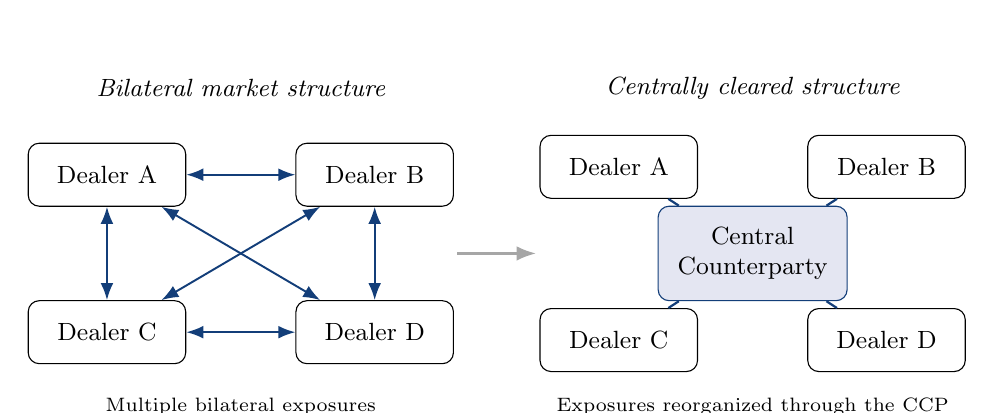
\begin{tikzpicture}[
    >=Latex,
    dealer/.style={
        draw,
        rounded corners,
        minimum width=20mm,
        minimum height=8mm,
        align=center,
        font=\small
    },
    ccp/.style={
        draw=FinanceBlue,
        fill=FinanceBlue!8,
        rounded corners,
        minimum width=24mm,
        minimum height=12mm,
        align=center,
        font=\small
    },
    bilateral/.style={
        Latex-Latex,
        line width=0.7pt,
        draw=FinanceBlue
    },
    title/.style={
        font=\small\itshape
    }
]

% Left panel: bilateral structure
\node[title] at (2.5,3.5) {Bilateral market structure};

\node[dealer] (A1) at (0.8,2.4) {Dealer A};
\node[dealer] (B1) at (4.2,2.4) {Dealer B};
\node[dealer] (C1) at (0.8,0.4) {Dealer C};
\node[dealer] (D1) at (4.2,0.4) {Dealer D};

\draw[bilateral] (A1) -- (B1);
\draw[bilateral] (A1) -- (C1);
\draw[bilateral] (A1) -- (D1);
\draw[bilateral] (B1) -- (C1);
\draw[bilateral] (B1) -- (D1);
\draw[bilateral] (C1) -- (D1);

\node[align=center, font=\scriptsize]
at (2.5,-0.55)
{Multiple bilateral exposures};

% Arrow between structures
\draw[->, line width=0.9pt, gray!70]
(5.25,1.4) -- (6.25,1.4);

% Right panel: centrally cleared structure
\node[title] at (9.0,3.5) {Centrally cleared structure};

\node[dealer] (A2) at (7.3,2.5) {Dealer A};
\node[dealer] (B2) at (10.7,2.5) {Dealer B};
\node[dealer] (C2) at (7.3,0.3) {Dealer C};
\node[dealer] (D2) at (10.7,0.3) {Dealer D};

\node[ccp] (CCP) at (9.0,1.4) {Central\\Counterparty};

\draw[line width=0.8pt, FinanceBlue] (A2) -- (CCP);
\draw[line width=0.8pt, FinanceBlue] (B2) -- (CCP);
\draw[line width=0.8pt, FinanceBlue] (C2) -- (CCP);
\draw[line width=0.8pt, FinanceBlue] (D2) -- (CCP);

\node[align=center, font=\scriptsize]
at (9.0,-0.55)
{Exposures reorganized through the CCP};

\end{tikzpicture}

\caption{Bilateral and centrally cleared counterparty relationships}

\label{fig:ch11-bilateral-central-clearing}

\end{figure}

Central clearing can also support multilateral netting across cleared positions. Obligations that would otherwise remain in separate bilateral relationships can be offset within the clearing system, reducing some gross exposures.

Central clearing therefore redistributes counterparty risk rather than eliminating it. Counterparty relationships become organized around the CCP rather than dispersed across many bilateral pairs, making the CCP a central node in the cleared market.

%========================================================
% Summary
%========================================================

\TailModule{summary}{Summary}

Derivative markets provide an institutional framework
for trading contracts whose cash flows depend on
underlying assets, rates, indices, or specified
events. These contracts create contingent claims
that allocate payments across possible future states.
By separating selected risk exposures from broader
business and financial positions, derivatives
facilitate risk transfer and sharing among market
participants. The range of attainable contingent
claims depends on the available traded instruments
and the completeness of the market.

Prices of contingent claims are linked through
no-arbitrage relationships among traded positions.
Payoff dominance imposes restrictions on relative
prices, while claims with identical state-contingent
payoffs must have the same current price. When a
claim can be replicated by a portfolio of traded
securities, its price must equal the cost of that
portfolio. The availability of traded instruments
therefore determines which claims can be replicated
exactly and, for claims that cannot, the range of
prices consistent with no-arbitrage.

Derivative-market architecture shapes trading,
settlement, and counterparty risk management.
Exchange-traded and OTC markets differ in
standardization and contractual flexibility.
Margin requirements, collateral, and netting
manage counterparty exposure, while central
clearing reorganizes bilateral exposures through
a central counterparty. These arrangements
redistribute risk without eliminating it.

%========================================================
% Key Terms
%========================================================

\TailModule{keyterms}{Key Terms}
Contingent claims; state-contingent payoffs;
exposure decomposition; risk unbundling; risk sharing;
market completeness; financial innovation;
law of one price; arbitrage; payoff dominance;
replication; synthetic positions;
exchange-traded derivatives; over-the-counter (OTC)
derivatives; liquidity; price discovery;
counterparty exposure; margin requirements;
collateral and netting; central clearing and
central counterparty (CCP).

%========================================================
% Financial AI Lab
%========================================================

\TailModule{aiprompt}{Financial AI Lab}

%========================================================
% Additional Financial AI Lab exercises
%========================================================

%========================================================
% Financial AI Lab
%========================================================


\textbf{Lab: Audit Counterparty Exposure and Risk
Management in Derivative Markets}

Ask an AI system to assess the counterparty exposure
of a firm's OTC derivatives portfolio. Consider a
firm with the following positions, valued from the
firm's perspective on the same date. All amounts
are measured in RMB millions.

\begin{center}
\begin{tabular}{lcc}
\toprule
\textbf{Counterparty}
& \textbf{Contract}
& \textbf{Market Value} \\
\midrule
Dealer A & Contract 1 & $+6.0$ \\
Dealer A & Contract 2 & $-4.0$ \\
Dealer B & Contract 3 & $+3.0$ \\
\bottomrule
\end{tabular}
\end{center}

The two contracts with Dealer A are subject to
the same legally enforceable close-out netting
agreement. Dealer A has posted variation margin
of RMB~1.2 million to the firm, measured after
applicable collateral haircuts. The contract with
Dealer B is subject to a separate netting agreement,
and no collateral has been received.

Require the AI system to calculate the firm's
current unsecured counterparty exposure and
evaluate how different risk-management arrangements
affect this exposure.

Audit the answer in four stages.

\begin{enumerate}

\item \textbf{Calculate net counterparty exposure.}

Determine the net current exposure to each dealer
after applying legally enforceable netting.
Account for collateral received and explain why
positions with different counterparties cannot
automatically be offset against each other.

\item \textbf{Distinguish market risk from
counterparty credit risk.}

Explain how changes in underlying prices affect
the market value of the contracts and the firm's
counterparty exposure. Identify why a positive
replacement value creates exposure to the
counterparty's failure to perform.

\item \textbf{Evaluate margin and collateral
arrangements.}

Distinguish initial margin from variation margin.
Explain how daily mark-to-market and variation
margin transfers affect current exposure, while
initial margin provides protection against
potential future exposure during the close-out
period. Identify risks that may remain despite
collateralization.

\item \textbf{Assess the role of central clearing.}

Explain how interposing a central counterparty
changes the original bilateral relationships.
Discuss multilateral netting, margin requirements,
default resources, and the concentration of
counterparty risk within the clearing system.
Distinguish the redistribution of counterparty
risk from the elimination of market risk.

\end{enumerate}

The final report should verify the exposure
calculations, identify the legal and operational
assumptions underlying netting and collateral,
and distinguish risk reduction from risk transfer
and risk concentration.

%========================================================
% Discussion Questions
%========================================================

\TailModule{questions}{Discussion Questions}

\begin{enumerate}

\item How can a derivative modify a selected financial
exposure without changing the firm's underlying
business activity?

\item How does market completeness affect the ability
to replicate contingent claims, and what pricing
uncertainty may remain when exact replication is
not feasible?

\item Why can a customized OTC contract provide a
closer match to an underlying exposure while
increasing the importance of collateral, margin
requirements, and bilateral netting arrangements?

\item How does central clearing reorganize counterparty
relationships, and why does this make the central
counterparty's risk management and resilience
important?

\end{enumerate}

%========================================================
% Applied Problems
%========================================================

\TailModule{appprobs}{Applied Problems}

\begin{enumerate}

\item \textbf{State-contingent payoffs and forward hedging.}

A commodity producer expects to sell one unit of
a commodity at date $T$. The spot price at that
date may be 70, 100, or 140. The producer enters
a cash-settled short forward contract with a
delivery price of 100 and the same maturity.

\begin{enumerate}

\item Calculate the payoff of the short forward
position in each state.

\item Calculate the producer's combined cash flow
from the physical sale and the forward position
in each state.

\item Explain how the forward contract changes
the distribution of the producer's cash flows
across states.

\end{enumerate}


\item \textbf{Exposure decomposition and risk unbundling.}

A firm will purchase 500 units of an imported
commodity at date $T$. The commodity price in
foreign currency is $P_T$, and the domestic-currency
price of one unit of foreign currency is $S_T$.
The firm's domestic-currency purchase cost is

\[
C_T=500P_TS_T.
\]

\begin{enumerate}

\item Identify the two market risk factors affecting
the firm's purchase cost.

\item Explain how changes in each risk factor affect
the firm's domestic-currency cash outflow.

\item Suppose the firm uses a derivative linked
only to the commodity price $P_T$. Which exposure
is modified, and which exposure remains?

\end{enumerate}


\item \textbf{Replication of a contingent claim.}

Two securities are traded in a two-state market.
Their current prices and payoffs are as follows:

\begin{center}
\begin{tabular}{lccc}
\toprule
\textbf{Security}
& \textbf{Current Price}
& \textbf{Up State}
& \textbf{Down State} \\
\midruleSecurity A & 8 & 12 & 6 \\
Security B & 9 & 4 & 10 \\
\bottomrule
\end{tabular}
\end{center}

A contingent claim pays 20 in the up state and
2 in the down state.

\begin{enumerate}

\item Determine the holdings of securities A
and B required to replicate the contingent claim.

\item Identify which positions are long and
which are short.

\item Calculate the current cost of the
replicating portfolio.

\item Explain why the claim's current value
must equal the replication cost under the
no-arbitrage condition.

\end{enumerate}


\item \textbf{Arbitrage opportunities and price consistency.}

Consider two pairs of derivative claims.

For the first pair, claims A and B have identical
payoffs of 15 in state 1 and 8 in state 2. Their
current prices are 13 and 10, respectively.

For the second pair, claims C and D have the
same current price of 11. Their payoffs are:

\begin{center}
\begin{tabular}{lcc}
\toprule
\textbf{Claim}
& \textbf{State 1}
& \textbf{State 2} \\
\midrule
Claim C & 14 & 20 \\
Claim D & 12 & 20 \\
\bottomrule
\end{tabular}
\end{center}

\begin{enumerate}

\item For the first pair, identify the arbitrage
strategy and calculate its initial cash flow
and future net payoffs.

\item For the second pair, identify the arbitrage
strategy and calculate its initial cash flow
and future net payoffs.

\item Why does an investment with a high expected
return not necessarily constitute an arbitrage
opportunity?

\end{enumerate}


\end{enumerate}
%========================================================
% Further Reading
%========================================================

\TailModule{furtherread}{Further Reading}

\begin{itemize}

\item Duffie, Darrell, and Chi-Fu Huang (1985),
``Implementing Arrow-Debreu Equilibria by Continuous Trading of Few Long-Lived Securities,''
\emph{Econometrica}, 53(6), 1337--1356.

\end{itemize}

\ChapterTail{summary,keyterms,aiprompt,questions,appprobs,furtherread}


\part{Financial Institutions}
\chapter{Commercial Banks: Credit Intermediation and Liquidity Creation}
\label{chap:Commercial_Banks_Credit_Intermediation_and_Liquidity_Creation}

\begin{openingcase}{Why Can a Solvent Bank Still Run Out of Cash?}

Consider a bank that has RMB~100 billion of assets. Most of its assets are loans to households and firms, together with bonds that mature over several years. On the liability side, a large share of its funding consists of deposits that customers can withdraw on demand or at short notice. The bank also has equity capital that absorbs losses.

Suppose the bank's borrowers continue to repay and the bank remains solvent, with the value of its assets exceeding its liabilities. Even so, a sudden wave of deposit withdrawals can create an immediate funding need. Selling long-term assets quickly may require price concessions, while replacing deposits with market funding can become expensive or unavailable.

The same balance-sheet structure that allows the bank to provide liquid deposits while financing illiquid loans can also create vulnerability when withdrawals rise sharply.

\end{openingcase}


\begin{tcolorbox}[
  enhanced,
  colback=FinanceBlue!6,
  colframe=FinanceBlue,
  boxrule=0.6pt,
  sharp corners,
  left=8pt,
  right=8pt,
  top=7pt,
  bottom=7pt,
  before skip=1em,
  after skip=1.6em,
  title=\textbf{Core Questions},
  coltitle=white,
  colbacktitle=FinanceBlue,
  fonttitle=\bfseries,
  attach boxed title to top left={xshift=6pt,yshift=-2mm},
  boxed title style={
    boxrule=0pt,
    sharp corners,
    left=5pt,
    right=5pt,
    top=2pt,
    bottom=2pt
  }
]
\begin{enumerate}[
  leftmargin=*,
  label=\textcolor{FinanceBlue}{\textbf{\arabic*.}},
  itemsep=0.55em,
  topsep=0.2em
]


\item How does a commercial bank use its balance sheet to transform funding from depositors and other providers into loans and other financial assets?

\item Why can banks create value through information production and contract design, including screening, monitoring, and relationship lending?

\item How do maturity transformation, liquidity creation, leverage, and funding structure create value while exposing banks to credit, interest-rate, and liquidity risk?

\end{enumerate}
\end{tcolorbox}

\section{Bank Balance Sheets and Balance-Sheet Intermediation}

At its core, a commercial bank is a balance-sheet intermediary. It raises funds through deposits and other liabilities, uses those funds to acquire loans and other financial assets, and holds equity capital to absorb losses.

\subsection{The Bank Balance Sheet: Assets, Funding, and Transactions}

A bank's balance sheet shows the assets it holds and how those assets are financed. Commercial banks typically hold loans, securities, reserves, and other liquid assets. These positions are funded through deposits, wholesale and other debt, and equity capital.

The economic significance of the balance sheet lies in the composition and contractual characteristics of these positions. Loans expose the bank to borrower performance. Securities can provide income, liquidity, and collateral, while reserves and other liquid assets support payment settlement and short-term liquidity needs. On the funding side, deposits and wholesale borrowing differ in maturity, stability, repricing, and withdrawal conditions. Equity absorbs losses before creditor claims are impaired.

\begin{table}[H]

\centering

\caption{A simplified commercial-bank balance sheet}

\label{tab:ch12-simplified-bank-balance-sheet}

\begin{tabularx}{0.82\textwidth}{@{}X X@{}}

\toprule

\textbf{Assets} & \textbf{Liabilities and Equity} \\

\midrule

Loans to households and firms & Transaction and savings deposits \\

Government and other securities & Time deposits and certificates of deposit \\

Reserves and other liquid assets & Wholesale and market funding \\

& Equity capital \\

\bottomrule

\end{tabularx}

\end{table}

A commercial bank intermediates by holding claims on borrowers and other issuers while issuing its own liabilities to depositors and other fund providers. The assets and liabilities on the two sides can differ in maturity, liquidity, risk, and repricing characteristics. The two sides are managed jointly: lending decisions affect the size and composition of bank assets, while deposit flows, wholesale funding, and equity affect how those assets are financed and the bank's available liquidity and loss-absorbing capacity.

These interactions can be seen directly in bank transactions. When a bank grants a loan and credits the proceeds to a deposit account at the same bank, it records a new loan asset and a corresponding deposit liability.

\begin{example}{From Loan Origination to Settlement}{loan-origination-balance-sheet}

Before a new loan, a bank has the following simplified balance sheet, in millions of renminbi:

\begin{center}

\begin{tabular}{
@{\hspace{0.8em}}
p{0.25\textwidth} r
@{\hspace{2.0em}}
p{0.24\textwidth} r
@{\hspace{2.5em}}
}

\toprule

\multicolumn{2}{c}{\textbf{Assets}} &
\multicolumn{2}{c}{\textbf{Liabilities and Equity}} \\

\cmidrule(lr){1-2}\cmidrule(lr){3-4}

Loans & 70 & Deposits & 82 \\

Securities & 15 & Wholesale funding & 8 \\

Reserves & 15 & Equity & 10 \\

\midrule

\textbf{Total} & \textbf{100} &
\textbf{Total} & \textbf{100} \\

\bottomrule

\end{tabular}

\end{center}

The bank grants a new RMB~5 million loan and credits the borrower's deposit account. At origination,

\[
\Delta L=+5,
\qquad
\Delta D=+5.
\]

Total assets and total liabilities plus equity both increase to RMB~105 million. Equity is unchanged at origination.

Suppose the borrower then transfers the RMB~5 million deposit to an account at another bank. If the payment is settled through reserves and there are no offsetting inflows, the originating bank's deposit liability and reserves both decline by RMB~5 million. The loan remains on the asset side of the balance sheet.

\end{example}

Loan origination and payment settlement are distinct balance-sheet events. Creating a deposit at origination does not by itself provide the settlement assets needed if the funds subsequently leave the bank. A bank experiencing net deposit outflows may need to use liquid assets, obtain replacement funding, or adjust other positions.

\subsection{Bank Capital, Leverage, and Balance-Sheet Constraints}

Within this balance-sheet structure, equity capital is the residual claim on the bank's assets after liabilities have been met. Declines in asset value reduce equity before they affect creditor claims. If losses are sufficiently large to exhaust the capital buffer, creditors can become exposed to loss.

A simple balance-sheet measure of leverage is the asset-to-equity ratio $A/E$. A higher leverage ratio means that a larger asset position is supported by a given amount of equity. It also makes equity more sensitive to changes in asset value. When liabilities remain unchanged, losses on assets are reflected in equity, so a relatively small percentage decline in assets can produce a much larger percentage decline in equity.

\begin{example}{Leverage and Loss Absorption}{bank-leverage-loss}

A bank has RMB~100 billion of assets, RMB~92 billion of liabilities, and RMB~8 billion of equity. Its asset-to-equity ratio is

\[
100\div 8=12.5.
\]

Suppose asset values fall by 2\%, or RMB~2 billion, while liabilities remain unchanged. Equity declines from RMB~8 billion to RMB~6 billion, a 25\% reduction.

The example illustrates how leverage makes equity more sensitive than total assets to changes in asset value.

\end{example}

Capital is one of several constraints on bank balance-sheet expansion. Additional lending or other asset growth requires funding and may also increase demands on capital and liquidity. Prudential requirements can further limit leverage, risk-weighted exposures, liquidity positions, and concentrations of risk. Which constraint is most important depends on the bank's balance-sheet structure and market conditions.

These constraints influence the scale and composition of the balance sheet. Expanding lending increases credit exposure and may require additional funding and capital, while holding more liquid assets strengthens liquidity capacity but can reduce expected return. Greater reliance on short-term wholesale funding can provide flexible financing while increasing refinancing exposure.

\begin{tcolorbox}[
  enhanced,
  breakable,
  colback=white,
  colframe=FinanceBlue,
  boxrule=0.7pt,
  sharp corners,
  borderline west={2.2pt}{0pt}{FinanceBlue},
  title=\textbf{Financial Perspective: Capital and Liquidity Serve Different Functions},
  coltitle=white,
  colbacktitle=FinanceBlue,
  fonttitle=\bfseries,
  before skip=1.2em,
  after skip=1.2em
]

Capital absorbs losses when the value of bank assets declines. Liquidity provides the means to meet payments and withdrawals when they fall due.

A bank can have positive equity but insufficient liquid resources to meet immediate outflows. Conversely, a bank can hold substantial liquid assets while suffering losses large enough to weaken its capital position.

Capital and liquidity are related, but they address different forms of balance-sheet vulnerability.

\end{tcolorbox}



\section{Credit Assessment and Loan Decisions}

Loans enter the bank's balance sheet through a credit process that converts borrower information into lending decisions. Commercial banks use borrower-specific information alongside publicly available information to assess credit quality, set credit limits and loan terms, and review exposures as conditions change. Credit allocation is therefore an ongoing process rather than a single decision at origination.

The main information requirements and corresponding
lending decisions at each stage of a bank credit
relationship are summarized in
Table~\ref{tab:ch12-credit-process}.

\begin{table}[H]
\centering
\caption{Information and decisions over a bank credit relationship}
\label{tab:ch12-credit-process}
\begin{tabularx}{0.90\textwidth}{@{}p{0.22\textwidth} X X@{}}
\toprule
\textbf{Stage} & \textbf{Information focus} & \textbf{Bank decision} \\
\midrule
Initial assessment
& Repayment capacity, financial position, cash-flow stability, collateral, and business conditions
& Approve, reject, or limit the proposed exposure \\
Contract design
& Expected use of funds, repayment pattern, uncertainty, and protection available to the bank
& Set amount, maturity, repayment terms, pricing, collateral, and covenants \\
Monitoring and renewal
& Payment behavior, account activity, updated financial information, and changes in business conditions
& Maintain, expand, tighten, restructure, or discontinue the exposure \\
\bottomrule
\end{tabularx}
\end{table}

\subsection{Borrower Information and Credit Assessment}

Credit assessment evaluates the borrower's capacity to meet contractual obligations and the risk associated with the proposed exposure. The assessment draws on several sources of information, each of which provides evidence about a different aspect of credit quality.

Financial statements provide information about profitability, leverage, liquidity, and balance-sheet structure. Cash-flow records help assess whether operating inflows can support debt service, while repayment history and account activity provide evidence about observed payment behavior. Industry conditions, customer concentration, ownership structure, and the purpose of the loan can further affect expected repayment capacity. Collateral provides an additional source of recovery if contractual payments are not made as agreed.

Banks combine these inputs through financial analysis, scoring systems, statistical models, and professional judgment. The relative importance of each method varies across borrowers and loan types. Standardized information may support more comparable assessments, while borrower-specific information can become more important when repayment capacity depends on conditions that are difficult to capture through financial ratios alone.

The information is then translated into an internal credit assessment, which may take the form of a rating, risk grade, or other classification used in the bank's credit process. This assessment does not determine the lending decision mechanically. It provides a basis for decisions about the amount of credit, contractual terms, and the intensity of subsequent monitoring.

\begin{example}{From Borrower Information to Credit Assessment}{borrower-information-credit-assessment}

Two firms apply for comparable working-capital facilities. Both report annual sales of RMB~20 million and similar leverage ratios.

Firm A generates stable operating cash flows, maintains adequate debt-service capacity, and has a consistent repayment record. Firm B faces greater cash-flow volatility, has a narrower margin for meeting its debt obligations, and has a history of late payments.

The bank would generally assess Firm A as more creditworthy, assigning it a stronger internal credit grade and a lower estimated probability of default. Other things being equal, Firm A would be eligible for a larger credit limit, a lower lending spread, and less stringent collateral requirements than Firm B.

\end{example}



\subsection{Loan Terms, Credit Limits, and Exposure}

The credit assessment is then translated into a lending decision. The bank sets a credit limit and other loan terms that determine how much exposure can be created and how that exposure evolves over time. The main contractual terms and their implications for the bank's credit exposure are summarized in Table~\ref{tab:ch12-loan-terms-exposure}. Together, these terms determine the size, duration, and conditions of the bank's exposure to the borrower.

\begin{table}[htbp]

\centering

\caption{Selected loan terms and their effects on bank exposure}

\label{tab:ch12-loan-terms-exposure}

\begin{tabularx}{0.90\textwidth}{@{}p{0.26\textwidth} X@{}}

\toprule

\textbf{Loan term} &
\textbf{Exposure implication} \\

\midrule

Loan amount or credit limit &
Sets the maximum amount of credit available under the contract \\

Maturity &
Sets the horizon before repayment or renewal is required \\

Repayment structure &
Governs how the outstanding principal changes over time \\

Interest-rate structure &
Governs whether and how the contractual interest rate is reset \\

Collateral and covenants &
Provide contractual protection through pledged assets and restrictions or requirements on borrower actions \\

Drawing and renewal conditions &
Govern when additional funds may be drawn and whether credit continues beyond the current term \\

\bottomrule

\end{tabularx}

\end{table}

Repayment and drawing terms determine how the funded exposure evolves after credit has been granted. Let $B_t$ denote the outstanding principal at the end of period $t$, $D_t$ new drawings during the period, and $R_t$ principal repayments. A simple balance relation is

\begin{equation}
B_t=B_{t-1}+D_t-R_t.
\label{eq:ch12-loan-balance-dynamics}
\end{equation}

For a term loan, the principal is normally advanced at origination and subsequently declines as repayments are made. A revolving credit facility operates differently: the borrower may draw, repay, and draw again within a contractual credit limit. The credit limit is therefore distinct from the amount currently outstanding.

This distinction creates two related measures of exposure. \emph{Funded exposure} is the amount already advanced and still outstanding. An \emph{undrawn commitment} is the unused portion of a committed facility that may become funded if the borrower draws additional amounts in accordance with the contract. A rise in utilization can therefore increase the bank's funded exposure even when the contractual credit limit remains unchanged.

\begin{example}{A Revolving Credit Facility and Bank Exposure}{revolving-credit-exposure}

A firm receives a one-year revolving credit facility with a limit of RMB~10 million. At the beginning of the year, RMB~4 million is outstanding. During the next quarter, the firm draws another RMB~3 million and repays RMB~1 million. Using Equation~\ref{eq:ch12-loan-balance-dynamics},

\[
B_t=4+3-1=6
\]

million renminbi.

The bank therefore has RMB~6 million of funded exposure, while RMB~4 million remains undrawn under the facility. If the borrower later draws part of this unused amount, the funded exposure increases without any change in the contractual credit limit.

\end{example}

Loan terms establish the initial structure of the exposure, but borrower conditions can change after credit has been extended. New information may therefore lead the bank to review the exposure, reassess further drawings, and reconsider renewal decisions.

\subsection{Monitoring, Renewal, and Credit Adjustment}

Monitoring allows the bank to update its assessment using repayment performance, account activity, financial information, collateral values, covenant compliance, and changes in business conditions. Covenant compliance refers to whether the borrower continues to satisfy the restrictions and requirements specified in the loan contract.

Changes in these indicators can trigger a credit review. Missed payments, persistent weakness in operating cash flow, or a material covenant breach may indicate deterioration, while a stronger payment record or financial position may support the continuation of existing credit. The purpose of the review is to determine whether the bank's current exposure remains consistent with its updated assessment of the borrower.

Renewal provides a further decision point. The bank can combine current information with the borrower's performance over the life of the facility when deciding whether to continue, expand, reduce, or discontinue the credit arrangement. Information accumulated through the lending relationship can therefore affect subsequent credit decisions even when no payment default has occurred.

Credit adjustment depends on both the updated assessment and the rights available under the contract. During the life of a facility, the bank may, where permitted, restrict additional drawings or require specified protective actions. At renewal, it can reconsider the credit limit and other contractual terms. Monitoring and renewal therefore provide mechanisms through which changes in borrower conditions can be translated into changes in bank exposure.

\begin{example}{From Monitoring to Credit Adjustment}{monitoring-credit-adjustment}

A firm has a RMB~8 million revolving credit facility. Sales remain broadly stable, but operating cash inflows weaken, customer receivables rise, and utilization of the credit line increases from 40\% to 85\%. 

These developments do not by themselves imply default, but together they may trigger a credit review. The bank can examine the source of the cash-flow pressure, update its assessment of the borrower, and reconsider the existing exposure.

If the weakness appears temporary, the bank may maintain the facility. If the deterioration persists, it may, subject to the contract, restrict further drawings or require additional protection. At renewal, it may reduce the credit limit or decline to renew the full amount.

\end{example}

Credit decisions therefore affect not only the composition of bank assets but also the amount of funding that may be required to support them. This link leads to the bank's funding structure and liquidity management.

\section{Bank Funding and Liquidity Creation}

Commercial banks often fund longer-term and less liquid assets with liabilities that are shorter-term and more liquid. Liquidity creation depends on the bank's funding structure and its capacity to meet cash outflows as they occur.

\subsection{Deposit and Wholesale Funding}

The composition of bank funding matters because funding sources differ in withdrawal rights, maturity, repricing, and concentration. Commercial banks rely primarily on deposits and various forms of wholesale funding, and these sources can respond differently to changes in interest rates, market conditions, and confidence.

Deposits are liabilities of commercial banks, but their funding behavior differs across products and customers. Transaction and savings deposits may be available at short notice, while time deposits generally provide funding for a more defined period. Stability also depends on depositor concentration, insurance coverage, interest-rate sensitivity, and perceived bank risk. Retail deposits are often more dispersed, whereas large corporate or institutional balances can create more concentrated funding exposures.

Wholesale funding includes interbank borrowing, certificates of deposit, secured borrowing, and other market-based liabilities. It can supplement deposit funding when balance-sheet growth or payment flows create additional funding needs. Its usefulness depends not only on cost but also on maturity and rollover conditions: shorter-term funding requires more frequent refinancing and can become less available when market conditions deteriorate.

\begin{table}[H]

\centering

\caption{Funding sources and selected liquidity characteristics}

\label{tab:ch12-bank-funding-characteristics}

\begin{tabularx}{0.92\textwidth}{@{}p{0.23\textwidth} X X@{}}

\toprule

\textbf{Funding source} &
\textbf{Contractual feature} &
\textbf{Implication for bank funding} \\

\midrule

Transaction and savings deposits &
Generally available to customers at short notice, subject to product terms &
Stability depends on customer mix, concentration, interest rates, and confidence \\

Time deposits &
Funds remain for a specified maturity or notice period &
Funding is more predictable before maturity, while rollover decisions arise as maturity approaches \\

Certificates of deposit &
Tradable or nontradable bank liabilities with specified maturities &
Funding cost and rollover depend on market conditions and investor demand \\

Interbank borrowing &
Short-term borrowing from other financial institutions &
Provides flexible funding but can require frequent refinancing \\

Secured market funding &
Borrowing supported by pledged collateral &
Funding capacity depends on available collateral and financing terms \\

\bottomrule

\end{tabularx}

\end{table}

Funding structure is closely related to liquidity creation. Banks can fund relatively illiquid assets with liabilities that provide greater liquidity to their holders. Sustaining this structure requires sufficient liquidity capacity to meet withdrawals, maturing liabilities, and other cash outflows as they occur.

\subsection{Liquidity Capacity and Balance-Sheet Adjustment}

Many bank liabilities can require payment before the bank's assets mature. A bank's liquidity capacity depends on the resources that can be converted into settlement funds within the relevant time horizon. These resources can include cash and reserves, proceeds from marketable assets, and additional borrowing capacity.

A simple representation is

\begin{equation}
LC_t=C_t+M_t+F_t^{\mathrm{avail}},
\label{eq:ch12-liquidity-capacity}
\end{equation}

where $C_t$ denotes cash and reserves immediately available, $M_t$ the cash that can reasonably be raised from marketable assets within the horizon, and $F_t^{\mathrm{avail}}$ additional funding that can reasonably be obtained. To avoid double counting, the amounts attributed to asset sales and borrowing capacity should be adjusted when they rely on the same assets or collateral. Liquidity capacity therefore depends on both the time horizon and the conditions under which funds must be raised.

The amount of cash obtainable from an asset can differ from its reported market value. Transaction costs, settlement timing, price changes, and restrictions on the use of pledged assets can affect the proceeds from asset sales. Similarly, borrowing capacity can depend on the availability and value of collateral, counterparties' willingness to lend, and prevailing financing conditions.

When cash outflows occur, the bank can adjust both sides of its balance sheet. It can use reserves, sell marketable securities, obtain secured borrowing by pledging eligible assets as collateral, obtain other replacement funding, or reduce the growth of new assets. These responses meet liquidity needs through different channels and leave different balance-sheet positions afterward.

\begin{example}{Meeting a Deposit Outflow}{meeting-deposit-outflow}

A bank has RMB~6 billion of reserves, RMB~8 billion of marketable securities that are not already pledged as collateral, and RMB~4 billion of secured borrowing capacity supported by other eligible assets. It experiences a RMB~10 billion net deposit outflow.

One possible adjustment is to use RMB~6 billion of reserves and obtain RMB~4 billion of secured borrowing. Another is to use the reserves and sell RMB~4 billion of marketable securities. Both responses provide the required liquidity, but their balance-sheet effects differ.

The first response increases secured liabilities and encumbers assets as collateral. The second reduces the bank's holdings of marketable securities. Liquidity management therefore concerns not only meeting the current outflow but also the liquidity resources that remain available afterward.

\end{example}

Liquidity capacity determines how readily the bank can meet current cash outflows. Larger or more persistent outflows may require progressively greater balance-sheet adjustment.

\subsection{Funding Outflows and Liquidity Adjustment}

Funding outflows occur when deposits leave the bank or when maturing liabilities are repaid without replacement. Such outflows reduce bank funding and create a cash requirement unless they are offset by asset-side cash inflows or new funding.

Let $O_t$ denote funding outflows during a short horizon, $I_t$ cash received from maturing or sold assets, and $F_t$ new funding obtained during the same period. The resulting change in cash and reserves can be represented as

\begin{equation}
\Delta C_t=I_t+F_t-O_t.
\label{eq:ch12-liquidity-adjustment}
\end{equation}

The relation shows how funding outflows are transmitted to the bank's liquidity position. When asset-side cash inflows and new funding are insufficient to offset the outflow, cash and reserves decline. When replacement resources are sufficient, the bank can meet the outflow without drawing down its existing cash position.

The adjustment required depends not only on the amount of the outflow but also on its timing and concentration. The nonrenewal of a large wholesale liability may create a more immediate replacement need than a similar amount of withdrawals distributed across many depositors. The relevant issue is how much funding must be replaced within the available time horizon.

Anticipated funding needs can also affect balance-sheet decisions before an outflow occurs. A bank may lengthen funding maturities, preserve liquid assets, arrange additional borrowing capacity, or moderate new asset growth. These actions can reduce short-term liquidity pressure, although they may alter funding costs, expected returns, or balance-sheet flexibility.

Funding outflows can therefore change both the level of liquid resources and the composition of the balance sheet. Larger or more persistent adjustments can also affect funding costs, asset holdings, and other dimensions of bank risk.

\section{Integrated Bank Risk Management}

Bank risks interact through a common balance sheet. A shock to credit quality, interest rates, or funding can affect earnings, capital, and liquidity, while the resulting balance-sheet adjustments can create further exposures.

\subsection{Loan Losses, Earnings, and Capital}

Deterioration in the loan portfolio can reduce a bank's earnings and, through retained earnings, weaken its capital position. The transmission runs from the recognition of credit losses to current income and then to book equity.

A loan-loss provision is an expense that recognizes credit losses under the applicable accounting framework. Provision expense reduces current earnings, while the associated allowance reduces the net carrying amount of loans. If a loan is later written off against an existing allowance, both the gross loan balance and the allowance decline; the loss has already affected earnings through the earlier provision.

A simplified bank income statement can be written as

\begin{equation}
\textit{NI}=\textit{NII}+\textit{NIR}-\textit{OE}-P_L-T,
\label{eq:ch12-bank-net-income}
\end{equation}

where $\textit{NI}$ is net income, $\textit{NII}$ net interest income, $\textit{NIR}$ non-interest income, $\textit{OE}$ operating expense, $P_L$ loan-loss provision expense, and $T$ taxes. The equation highlights the direct effect of provision expense on bank earnings.

If dividends and other distributions are denoted by $D$ and new equity issued during the period by $\textit{NE}$, book equity evolves approximately as

\begin{equation}
E_1=E_0+\textit{NI}-D+\textit{NE},
\label{eq:ch12-equity-evolution}
\end{equation}
apart from other direct adjustments to equity. The two relations show the transmission mechanism:

\[
\begin{array}{c}
\text{\emph{Income statement}} \\[2pt]
\text{Loan deterioration}
\rightarrow
\text{Provision expense}
\rightarrow
\text{Lower net income}
\\[5pt]
\Downarrow
\\[-1pt]
\text{\emph{Balance sheet}} \\[2pt]
\text{Lower retained earnings}
\rightarrow
\text{Weaker equity position}
\end{array}
\]

\begin{example}{Provisioning, Earnings, and Capital}{provisioning-earnings-capital}

A bank begins the year with RMB~600 million of equity. Before provisions and taxes, it earns RMB~120 million. It records RMB~70 million of loan-loss provision expense and pays RMB~20 million in dividends. Ignore taxes and other equity adjustments.

Net income is RMB~50 million, and end-of-year equity is

\[
600+50-20=630
\]

million renminbi.

If provision expense rises to RMB~130 million under the same assumptions, net income becomes negative RMB~10 million and end-of-year equity falls to RMB~570 million. A larger recognized loan loss therefore reduces earnings and, other things equal, leaves the bank with less equity to absorb subsequent losses.

\end{example}

\subsection{Repricing and Asset--Liability Mismatch}

Interest-rate changes affect a bank through both an income channel and a valuation channel. The effects depend on when asset and liability rates are reset and on how sensitive their economic values are to changes in market yields.

Let $\textit{RSA}$ and $\textit{RSL}$ denote the amounts of interest-rate-sensitive
assets and liabilities, respectively, that are scheduled to reprice
within a given period. For a given balance-sheet position, the
approximate change in net interest income is

\begin{equation}
\Delta \textit{NII}\approx \textit{RSA}\cdot\Delta r_A
-RSL\cdot\Delta r_L,
\end{equation}
where $\Delta r_A$ and $\Delta r_L$ represent the changes in the
corresponding asset and liability rates. If these rates move by
approximately the same amount, so that
$\Delta r_A\approx\Delta r_L\approx\Delta r$, the expression
simplifies to

\begin{equation}
\Delta \textit{NII}\approx (\textit{RSA}-\textit{RSL})\Delta r
=G\Delta r.
\label{eq:ch12-net-interest-income-gap}
\end{equation}

The repricing gap, $G$, measures the difference between
rate-sensitive assets and liabilities. A positive gap implies
that an increase in interest rates tends to raise net interest
income, whereas a negative gap implies the opposite.

The approximation is intentionally simple. Deposit rates may adjust less than one-for-one with market rates, loans may reset only at specified dates or against different benchmark rates, and customer behavior can change outstanding balances. The repricing gap provides a first approximation to short-horizon income sensitivity rather than a complete measure of interest-rate exposure.

Economic-value analysis considers a different dimension of the mismatch. Fixed-rate assets and liabilities can differ in their sensitivity to changes in market yields even when their near-term cash flows do not change. Let $D_A$ and $D_L$ denote the effective durations of assets and liabilities, and let $A$ and $L$ denote their current economic values. The duration gap is

\begin{equation}
D_{GAP}=D_A-\frac{L}{A}D_L.
\label{eq:ch12-duration-gap}
\end{equation}

Effective duration measures the approximate percentage sensitivity of value to a small change in yield. For a small parallel change in market yields,

\begin{equation}
\Delta E\approx -A\,D_{GAP}\,\Delta y,
\label{eq:ch12-duration-gap-equity}
\end{equation}

where $\Delta E$ is the resulting change in the economic value of equity. A positive duration gap therefore implies that a rise in yields can reduce economic equity value under the stated approximation.

\begin{tcolorbox}[
  enhanced,
  breakable,
  colback=white,
  colframe=FinanceBlue,
  boxrule=0.7pt,
  sharp corners,
  borderline west={2.2pt}{0pt}{FinanceBlue},
  title=\textbf{Financial Perspective: Income and Economic-Value Effects Can Differ},
  coltitle=white,
  colbacktitle=FinanceBlue,
  fonttitle=\bfseries,
  before skip=1.2em,
  after skip=1.2em
]

The same interest-rate movement can affect bank income and economic value in different directions. For example, a rise in rates may increase near-term net interest income while reducing the economic value of equity.

\end{tcolorbox}

\subsection{Risk Interactions through the Balance Sheet}

Bank risks interact because credit losses, interest-rate movements, and funding shocks affect the same balance sheet.

A shock in one area can alter exposures in another. Loan losses can weaken earnings and capital; interest-rate movements can change both asset values and funding costs; and funding outflows can require asset sales or replacement borrowing. These responses can then affect collateral availability, realized gains or losses, funding costs, and the bank's capacity to absorb further shocks.

The strength of these interactions depends on the composition of assets and liabilities, funding maturity, collateral availability, hedging, and the bank's initial capital and liquidity position.

\begin{figure}[H]
\centering

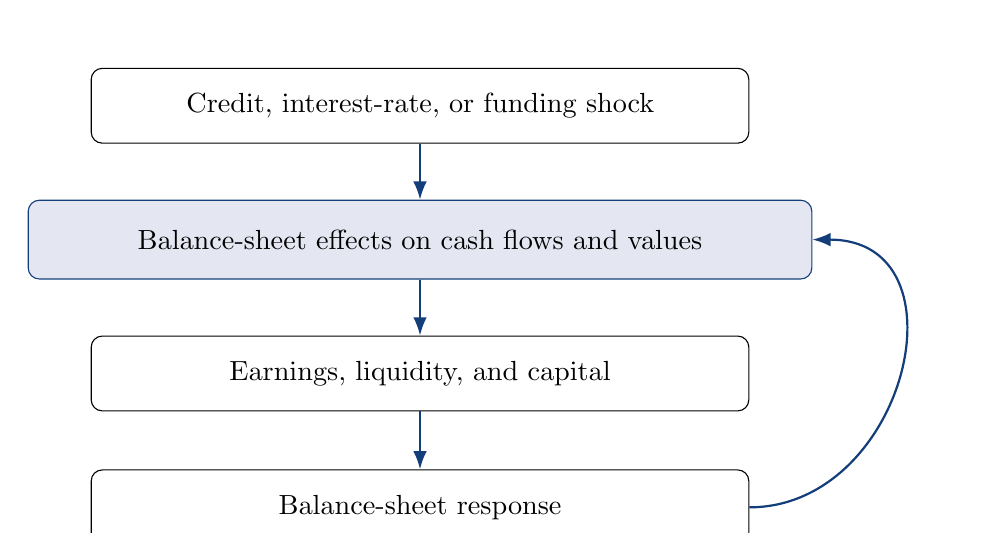
\begin{tikzpicture}[
  >=Latex,
  box/.style={
    draw,
    rounded corners,
    align=center,
    text width=8cm,
    minimum height=0.95cm,
    inner sep=5pt
  },
  main/.style={
    draw=FinanceBlue,
    fill=FinanceBlue!8,
    rounded corners,
    align=center,
    text width=9.6cm,
    minimum height=1.0cm,
    inner sep=5pt
  },
  flow/.style={
    -Latex,
    line width=0.8pt,
    FinanceBlue
  }
]

\node[box] (shock) at (0,3.0)
{Credit, interest-rate, or funding shock};

\node[main] (bs) at (0,1.3)
{Balance-sheet effects on cash flows and values};

\node[box] (capacity) at (0,-0.4)
{Earnings, liquidity, and capital};

\node[box] (adjustment) at (0,-2.1)
{Balance-sheet response};

\draw[flow] (shock) -- (bs);
\draw[flow] (bs) -- (capacity);
\draw[flow] (capacity) -- (adjustment);

\draw[flow]
(adjustment.east)
.. controls +(2.0,0) and +(2.0,0) ..
(bs.east);

\end{tikzpicture}

\caption{Risk transmission and balance-sheet adjustment within a commercial bank}
\label{fig:ch12-integrated-risk-interactions}
\end{figure}
Balance-sheet adjustments can therefore change the bank's subsequent exposure to credit, interest-rate, and funding risk.

\subsection[Capital Response and Balance-Sheet Adjustment]
{Capital Response and Balance-Sheet Adjustment}

Credit losses reduce book equity, while rapid asset growth
can lower the equity-to-assets ratio if equity does not grow
proportionately. A bank may strengthen its capital position
by retaining earnings or issuing new equity, reducing its
asset base, or combining these measures. A simple,
unweighted measure of capitalization is

\begin{equation}
k=\frac{E}{A},
\end{equation}
where $E$ denotes book equity and $A$ total assets.
Holding assets constant, an increase in equity raises the
ratio; holding equity constant, a reduction in assets has
the same effect.

Equity can be strengthened by retaining earnings, reducing distributions, or issuing new shares. Asset adjustment can include slowing new lending, allowing assets to mature without replacement, or selling loans and securities. These choices differ in timing and economic cost and can also change future earnings and the composition of the balance sheet.

Suppose a bank with initial equity $E_0$ and assets $A_0$ recognizes an asset loss $L_s$. If liabilities are unchanged when the loss is recognized,

\begin{equation}
E_1=E_0-L_s,
\label{eq:ch12-capital-after-loss}
\end{equation}
and post-loss assets are

\begin{equation}
A_1=A_0-L_s.
\end{equation}

If no new equity is raised and the bank seeks a target ratio $k^{*}$, the asset level consistent with that target is

\begin{equation}
A^{*}=\frac{E_1}{k^{*}}.
\label{eq:ch12-assets-consistent-capital-ratio}
\end{equation}

When $A_1>A^{*}$, the difference $A_1-A^{*}$ gives the asset reduction required under these simplified assumptions.

\begin{example}{Two Paths to Restore a Capital Ratio}{capital-response-paths}

A bank has RMB~100 billion of assets and RMB~8 billion of equity. It recognizes an RMB~2 billion asset loss, leaving RMB~98 billion of assets and RMB~6 billion of equity. Its equity-to-assets ratio falls from 8\% to approximately 6.12\%.

Suppose management seeks to restore an 8\% ratio.

One path is to issue new equity. If the proceeds remain on the balance sheet, an equity issue of RMB~2 billion raises assets to RMB~100 billion and equity to RMB~8 billion:

\[
\frac{8}{100}=8\%.
\]

A second path is to raise no new equity and reduce assets. With equity remaining at RMB~6 billion, the asset level consistent with an 8\% ratio is

\[
\frac{6}{0.08}=75
\]

billion renminbi.

The bank would therefore need to reduce assets by RMB~23 billion from their post-loss level. The two responses restore the same ratio but leave different balance-sheet positions.

\end{example}

Capital adjustment can therefore affect not only the capital ratio but also the bank's future earnings, liquidity, funding needs, and risk exposures.

%========================================================
% Summary
%========================================================

\TailModule{summary}{Summary}

A commercial bank is a balance-sheet intermediary. It holds loans, securities, reserves, and other assets while funding them with deposits, wholesale liabilities, and equity. Loan origination can create a loan asset and a deposit liability simultaneously, while subsequent payments can shift deposits and reserves across banks. Equity absorbs asset losses before creditor claims are impaired, and leverage increases the sensitivity of equity to changes in asset value.

Bank credit decisions evolve over time. Borrower information supports credit assessment, while loan terms and limits determine the size and structure of exposure. Monitoring provides updated information after origination, and renewal or contractual adjustment can change the bank's exposure as borrower conditions change.

Bank funding combines deposits with wholesale liabilities that differ in maturity, concentration, repricing, and withdrawal conditions. Liquidity creation arises when relatively liquid liabilities fund assets that are less liquid or longer dated. Liquidity management therefore depends on the resources available to meet cash outflows and on the balance-sheet adjustments used when funding conditions change.

Bank risks interact through the common balance sheet. Loan deterioration can reduce earnings and capital, interest-rate movements can affect both net interest income and economic value, and funding outflows can use liquidity resources or require replacement funding. Responses to one pressure can alter exposure to another. Capital can be rebuilt through retained earnings or new equity, while asset adjustment can change the size and composition of the balance sheet, with consequences for future earnings, liquidity, and risk.

%========================================================
% Mind Map
%========================================================

\TailModule{mindmap}{Mind Map}

\begin{figure}[H]
\centering
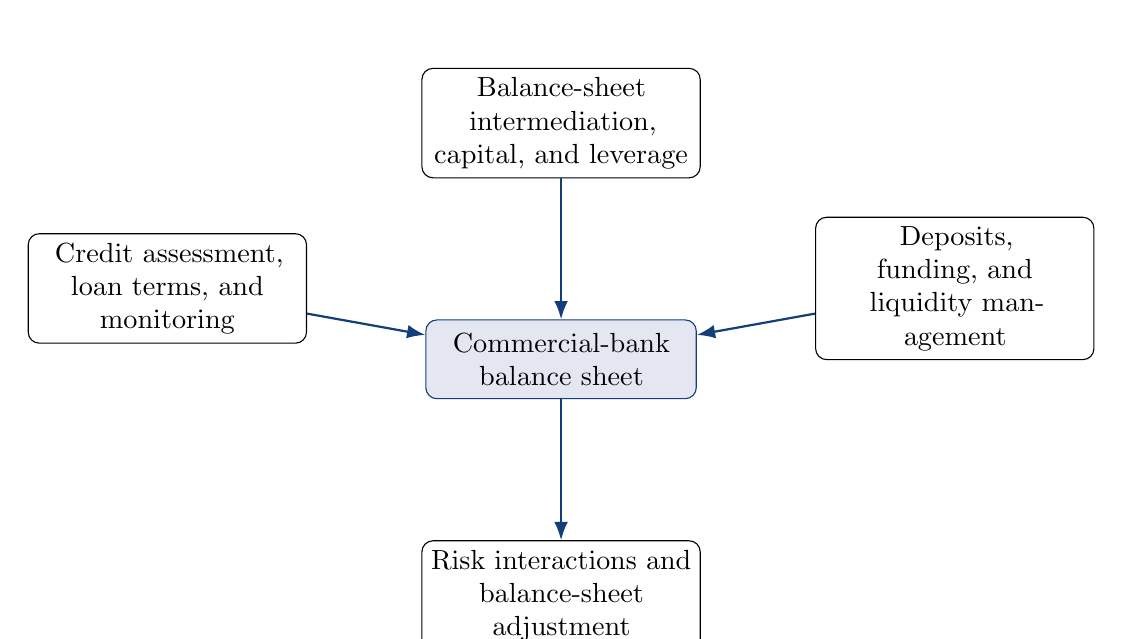
\begin{tikzpicture}[
  >=Latex,
  center/.style={
    draw=FinanceBlue,
    fill=FinanceBlue!8,
    rounded corners,
    align=center,
    text width=3.2cm,
    minimum height=1.0cm
  },
  box/.style={
    draw,
    rounded corners,
    align=center,
    text width=3.3cm,
    minimum height=0.95cm
  },
  flow/.style={-Latex, line width=0.8pt, FinanceBlue}
]

\node[center] (bank) at (0,0) {Commercial-bank\\balance sheet};

\node[box] (balance) at (0,3.0)
{Balance-sheet intermediation,\\capital, and leverage};

\node[box] (credit) at (-5.0,0.9)
{Credit assessment,\\loan terms, and monitoring};

\node[box] (funding) at (5.0,0.9)
{Deposits, funding, and\\liquidity management};

\node[box] (risk) at (0,-3.0)
{Risk interactions and\\balance-sheet adjustment};

\draw[flow] (balance) -- (bank);
\draw[flow] (credit) -- (bank);
\draw[flow] (funding) -- (bank);
\draw[flow] (bank) -- (risk);

\end{tikzpicture}
\caption*{Commercial banking links credit decisions, funding, liquidity, and capital through a common balance sheet.}
\end{figure}

%========================================================
% Key Terms
%========================================================

\TailModule{keyterms}{Key Terms}

Commercial bank; balance-sheet intermediation; deposits; wholesale funding;
equity capital; leverage; credit assessment; credit limit; funded exposure;
undrawn commitment; loan monitoring; loan renewal; funding maturity;
liquidity creation; liquidity capacity; funding outflows; net interest income;
repricing gap; asset--liability mismatch; duration gap; economic value of equity;
capital ratio; balance-sheet adjustment.

%========================================================
% Financial AI Lab
%========================================================

\TailModule{aiprompt}{Financial AI Lab}

\textbf{Lab: Audit an Integrated Bank Balance-Sheet Analysis}

Ask an AI system to analyze a simplified commercial bank with loans, securities,
reserves, deposits, wholesale funding, and equity. Provide information on a
borrower credit review, a deposit outflow, and a change in market interest rates.

Evaluate the analysis in four stages.

\begin{enumerate}

\item \textbf{Check the balance-sheet identity.}
Verify that assets equal liabilities plus equity after loan origination,
payment settlement, funding outflows, and recognized losses. For each change,
identify the corresponding balance-sheet entry.

\item \textbf{Evaluate the credit decision.}
Introduce weaker borrower cash-flow information and ask whether the existing
credit limit should be maintained. Assess the reasoning about repayment
capacity, contractual terms, and exposure rather than accepting an unsupported
default probability.

\item \textbf{Separate liquidity from capital.}
Apply a deposit outflow and identify the resources that can provide cash within
the specified horizon. Check whether the analysis distinguishes liquidity
capacity from the economic value of the bank's assets and from its capital
position.

\item \textbf{Trace risk interactions.}
Apply an interest-rate change and a loan-loss provision. Examine the effects on
net interest income, economic value, earnings, and capital, and verify that any
proposed balance-sheet adjustment remains internally consistent.

\end{enumerate}

%========================================================
% Discussion Questions
%========================================================

\TailModule{questions}{Discussion Questions}

\begin{enumerate}

\item Why does a commercial bank operate as a balance-sheet intermediary rather than simply transferring existing deposits from savers to borrowers?

\item How can borrower-specific information affect both the amount of credit a bank is willing to provide and the contractual terms attached to that credit?

\item Why can a committed credit limit differ from the bank's current funded exposure?

\item How do funding concentration, maturity, and interest-rate sensitivity affect a bank's liquidity management?

\item How can the same interest-rate increase raise near-term net interest income while reducing the economic value of equity?

\item Why can an asset sale undertaken to raise liquidity also affect earnings or capital through realized gains or losses?

\end{enumerate}

%========================================================
% Applied Problems
%========================================================

\TailModule{appprobs}{Applied Problems}

\begin{enumerate}

\item \textbf{Loan origination and payment settlement.}

A bank initially has RMB~80 million of loans, RMB~15 million of securities, and RMB~5 million of reserves. It is funded with RMB~82 million of deposits, RMB~8 million of wholesale funding, and RMB~10 million of equity.

\begin{enumerate}

\item The bank grants a new RMB~4 million loan and credits the borrower's
deposit account. Show the immediate balance-sheet effect.

\item The borrower transfers the RMB~4 million deposit to another bank.
If settlement reduces reserves by RMB~4 million, show the resulting balance sheet.

\item If the bank wants to restore reserves to RMB~3 million, identify two
balance-sheet adjustments that could provide the required cash.

\end{enumerate}

\item \textbf{Credit limits and exposure.}

A firm has a RMB~12 million revolving facility. The beginning balance is RMB~5 million. During the quarter the firm draws RMB~4 million and repays RMB~2 million.

\begin{enumerate}
\item Calculate the ending funded exposure.
\item Calculate the undrawn amount under the credit limit.
\item Suppose operating cash flow weakens and receivables rise. Explain two ways the bank could adjust the exposure without requiring immediate repayment of the full outstanding balance.
\item Explain why raising the loan rate is not the only possible response to a weaker credit assessment.
\end{enumerate}

\item \textbf{Funding outflow and liquidity capacity.}

A bank has RMB~7 billion of reserves, RMB~9 billion of securities that can be converted into RMB~8.5 billion of cash within the day, and RMB~3 billion of available secured borrowing capacity supported by other collateral. It experiences a RMB~14 billion net deposit outflow.

\begin{enumerate}
\item Calculate liquidity capacity under Equation~(\ref{eq:ch12-liquidity-capacity}).
\item Is the stated capacity sufficient to meet the outflow?
\item If the bank uses all reserves and RMB~7 billion of cash from securities sales, what liquid resources remain under the stated assumptions?
\item Explain how the answer would change if part of the securities portfolio were already pledged as collateral.
\end{enumerate}


\item \textbf{Repricing and economic-value exposure.}


Over the next year, a bank has RMB~85 billion of rate-sensitive assets and RMB~70 billion of rate-sensitive liabilities.

\begin{enumerate}
\item Calculate the repricing gap.
\item Estimate the change in annual net interest income if relevant rates rise by 80 basis points using Equation~(\ref{eq:ch12-net-interest-income-gap}).
\item The same bank has assets of RMB~100 billion, liabilities of RMB~92 billion, asset duration of 4.2, and liability duration of 1.8. Calculate the duration gap.
\item Estimate the first-order change in economic value of equity for a 50-basis-point increase in yields.
\item Explain why the income and economic-value measures need not move in the same direction over the same horizon.
\end{enumerate}

\item \textbf{Capital response and balance-sheet adjustment.}

A bank has RMB~120 billion of assets and RMB~9.6 billion of equity. It recognizes a RMB~2.4 billion loss.

\begin{enumerate}
\item Calculate the initial and post-loss equity-to-assets ratios, assuming the loss reduces assets and equity by the same amount.
\item If the bank seeks an 8\% simple equity-to-assets ratio and raises no new equity, calculate the asset level consistent with that ratio.
\item Calculate the implied asset reduction from the post-loss balance sheet.
\item Identify two alternatives to balance-sheet contraction and explain one limitation of each.
\end{enumerate}

\end{enumerate}

%========================================================
% Data Application
%========================================================

\TailModule{dataapp}{Data Application}

\textbf{Commercial-Bank Balance Sheets, Funding, and Capital in China}

Use an authoritative Chinese source such as the People's Bank of China,
the National Financial Regulatory Administration, or the published financial
statements of a listed commercial bank. Select one bank or a consistent
banking-sector series and collect at least five years of data on major assets,
deposits, other funding, liquid assets where separately reported, and equity.

Construct ratios that address three questions: How are bank assets allocated?
How is the balance sheet funded? How much book equity supports the asset base?
Useful measures may include loans to total assets, deposits to total liabilities,
liquid assets to total assets, and book equity to total assets. Use consistent
accounting definitions across the sample period and distinguish accounting
equity from regulatory capital measures.

Identify one period in which asset growth, deposit growth, funding composition,
or equity changed materially. Trace the change through the balance-sheet
identity rather than interpreting a single ratio in isolation. If loans grew
faster than deposits, identify which other liabilities or equity financed the
difference. If equity grew more slowly than assets, calculate the resulting
change in simple leverage.

If comparable data are available for two banks, compare their asset mix,
deposit structure, reliance on nondeposit funding, and liquid-asset positions.
Discuss how these differences could affect their balance-sheet responses to a
hypothetical funding outflow or interest-rate change. Do not treat reported
liquid assets alone as a complete measure of liquidity capacity.

Report the institution, sample period, accounting definitions, source documents,
and any transformations used in the analysis.

%========================================================
% Case Analysis
%========================================================

\TailModule{caseanalysis}{Case Analysis}

\textbf{Case: Silicon Valley Bank---An Individual-Bank Balance-Sheet Analysis}

Silicon Valley Bank was closed by the California Department of Financial
Protection and Innovation on March 10, 2023, and the Federal Deposit Insurance
Corporation was appointed receiver. The Federal Reserve's subsequent review
identified rapid balance-sheet growth, a concentrated business model, heavy
reliance on uninsured deposits, and weaknesses in liquidity and interest-rate
risk management.\footnote{Board of Governors of the Federal Reserve System, \emph{Review of the Federal Reserve's Supervision and Regulation of Silicon Valley Bank}, April 2023; Federal Deposit Insurance Corporation, \emph{Failed Bank Information for Silicon Valley Bank}, 2023.}

As market interest rates rose during 2022, the market value of SVB's
long-duration fixed-rate securities declined. At the same time, weaker
venture-capital activity reduced deposit inflows, while some technology and
venture-backed clients drew down deposits to finance their operations. On
March 8, 2023, SVB Financial Group announced a balance-sheet restructuring
that included the sale of a large available-for-sale securities portfolio,
recognition of an after-tax loss, and a planned capital raise.

Analyze the episode at the level of the bank's balance sheet. Separate four
questions: How did the securities portfolio respond to higher market interest
rates? How did the composition of deposits affect the stability of funding?
Which assets or funding sources could provide liquidity within the required
time horizon? How did the realized loss affect the bank's capital position,
and how was the planned capital raise intended to respond?

Then trace one interaction among these dimensions. For example, an asset saleundertaken to raise liquidity can convert an unrealized decline in market value
into a realized loss that reduces earnings and capital. The episode therefore
illustrates how interest-rate exposure, funding outflows, liquidity adjustment,
and capital can interact through the same balance sheet.

The analysis here remains at the level of the individual bank. System-wide
contagion, emergency liquidity support, and prudential regulation are examined
in later chapters.

\emph{Primary sources: Board of Governors of the Federal Reserve System,
Review of the Federal Reserve's Supervision and Regulation of Silicon Valley
Bank, April 2023; Federal Deposit Insurance Corporation, Failed Bank Information
for Silicon Valley Bank, 2023; SVB Financial Group, SEC filings, March 2023.}

%========================================================
% Further Reading
%========================================================

\TailModule{furtherread}{Further Reading}

\begin{itemize}

\item Berger, Allen N., and Gregory F. Udell (1995),
``Relationship Lending and Lines of Credit in Small Firm Finance,''
\emph{The Journal of Business}, 68(3), 351--381.

\item Kashyap, Anil K., Raghuram Rajan, and Jeremy C. Stein (2002),
``Banks as Liquidity Providers: An Explanation for the Coexistence of Lending and Deposit-Taking,''
\emph{The Journal of Finance}, 57(1), 33--73.

\item Drechsler, Itamar, Alexi Savov, and Philipp Schnabl (2021),
``Banking on Deposits: Maturity Transformation without Interest Rate Risk,''
\emph{The Journal of Finance}, 76(3), 1091--1143.

\end{itemize}

\ChapterTail{summary,mindmap,keyterms,aiprompt,questions,appprobs,dataapp,caseanalysis,furtherread}

\chapter{Investment Banks: Capital Raising and Capital-Market Intermediation}
\label{chap:Investment_Banks_Capital_Raising_and_Capital_Market_Intermediation}

\begin{openingcase}{Why Does Direct Finance Need Investment Banks?}

A rapidly growing company plans to raise RMB~6 billion by selling new shares to public investors. Its financial statements have been audited, a prospectus can disclose the relevant information, and investors will ultimately hold the shares issued by the company itself.

Yet the company does not approach investors on its own. It hires an investment bank and pays substantial fees for its services. The bank becomes closely involved in preparing, pricing, and distributing the issue, and may also assume part of the risk associated with the offering.

\end{openingcase}

\begin{tcolorbox}[
  enhanced,
  colback=FinanceBlue!6,
  colframe=FinanceBlue,
  boxrule=0.6pt,
  sharp corners,
  left=8pt,
  right=8pt,
  top=7pt,
  bottom=7pt,
  before skip=1em,
  after skip=1.6em,
  title=\textbf{Core Questions},
  coltitle=white,
  colbacktitle=FinanceBlue,
  fonttitle=\bfseries,
  attach boxed title to top left={xshift=6pt,yshift=-2mm},
  boxed title style={
    boxrule=0pt,
    sharp corners,
    left=5pt,
    right=5pt,
    top=2pt,
    bottom=2pt
  }
]
\begin{enumerate}[
  leftmargin=*,
  label=\textcolor{FinanceBlue}{\textbf{\arabic*.}},
  itemsep=0.55em,
  topsep=0.2em
]

\item Why do issuers use investment banks when securities already create direct claims between issuers and investors?

\item How do investment banks use information, reputation, valuation, distribution networks, and balance-sheet capacity to support securities issuance, trading, and strategic transactions?

\end{enumerate}
\end{tcolorbox}

\section{Capital-Market Intermediation and Certification}

Investment banks help issuers access capital markets without replacing the securities ultimately held by investors. Their role is distinct from the balance-sheet intermediation of commercial banks, which commonly fund borrower claims with deposits and other bank liabilities.

\subsection{Issuers, Investors, and Capital-Market Access}

Issuers enter capital markets with different financing needs. A growing firm may raise equity to finance investment without adding fixed repayment obligations, while a corporation may issue bonds to obtain term funding, refinance existing debt, or diversify its funding sources. Governments and financial institutions also issue securities under different financing objectives and contractual structures.

Capital-market access requires the financing need to be translated into a security that investors can evaluate and purchase. The issuer must provide relevant information, define the terms of the claim, reach potential investors, and set terms at which sufficient investor demand can be attracted. Legal, disclosure, and transaction costs also make the scale and design of the issue economically important.

Investment banks help connect these two sides of the market. They advise on the structure and timing of an issue, organize the preparation and distribution process, and gather information about investor demand. This coordination can reduce search and transaction costs while improving the flow of information between issuers and investors. Figure~\ref{fig:ch13-direct-finance-intermediation} summarizes these relationships.

\begin{figure}[H]

\centering

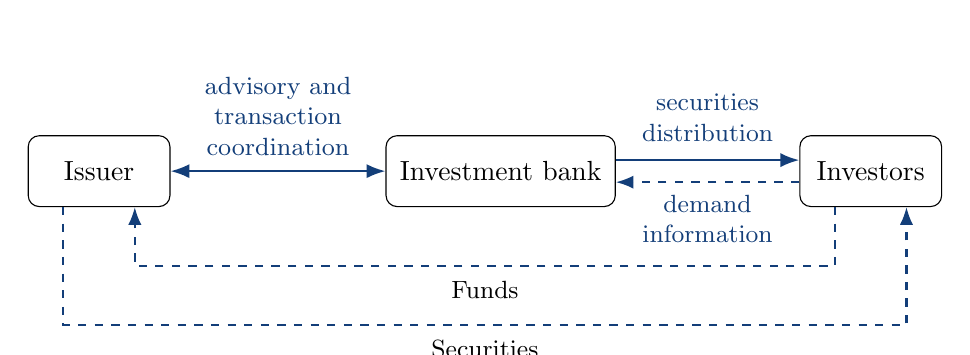
\begin{tikzpicture}[
  >=Latex,
  box/.style={
    draw,
    rounded corners,
    align=center,
    minimum width=1.8cm,
    minimum height=0.9cm,
    inner sep=5pt
  },
  service/.style={Latex-Latex, line width=0.85pt, FinanceBlue},
  claim/.style={Latex-Latex, dashed, line width=0.75pt, draw=gray!75}
]

\node[box] (issuer) at (-4.6,0) {Issuer};
\node[box] (ib) at (0.5,0) {Investment bank};
\node[box] (investors) at (5.2,0) {Investors};

\draw[service] (issuer) --
  node[midway, above=2pt, font=\small,
  text=FinanceBlue, align=center, text width=2.8cm]
  {advisory and transaction\\ coordination}
  (ib);

% Investment bank to investors: distribution
\draw[->, line width=0.85pt, FinanceBlue]
  ([yshift=0.14cm]ib.east) --
  node[midway, above=3pt, font=\small,
       text=FinanceBlue, align=center]
  {securities\\ distribution}
  ([yshift=0.14cm]investors.west);

% Investors to investment bank: demand information
\draw[->, dashed, line width=0.75pt, FinanceBlue]
  ([yshift=-0.14cm]investors.west) --
  node[midway, below=1pt, font=\small,
       align=center]
  { demand\\information}
  ([yshift=-0.14cm]ib.east);

% Funds: Issuer -> Investors
\coordinate (funds-start) at
  ($(investors.south west)!0.25!(investors.south east)$);

\coordinate (funds-end) at
  ($(issuer.south west)!0.75!(issuer.south east)$);

\coordinate (funds-level) at
  ($(funds-start)!0.5!(funds-end)+(0,-0.75cm)$);

\draw[->, dashed, line width=0.75pt, FinanceBlue]
  (funds-start)
  -- ++(0,-0.75cm)
  -| (funds-end);

\node[below=2pt, font=\small] at (funds-level) {Funds};

% Funds: Investors -> Issuer
\coordinate (funds-start) at
  ($(investors.south west)!0.75!(investors.south east)$);

\coordinate (funds-end) at
  ($(issuer.south west)!0.25!(issuer.south east)$);

\coordinate (funds-level) at
  ($(funds-start)!0.5!(funds-end)+(0,-1.5cm)$);

\draw[->, dashed, line width=0.75pt, FinanceBlue]
  (funds-end)
  -- ++(0,-1.5cm)
  -| (funds-start);

\node[below=2pt, font=\small] at (funds-level) {Securities};
  
\end{tikzpicture}

\caption{Investment-bank support for capital-market access}

\label{fig:ch13-direct-finance-intermediation}

\end{figure}


\subsection[Due Diligence, Information Certification, and Reputation]{Due Diligence, Information Certification, and\\ Reputation}

Securities issuance depends on credible disclosure about the issuer, the security, and the risks of the transaction. Due diligence supports this process by examining information that may affect disclosure, valuation, or execution. It may include reviews of financial statements, business plans, material contracts, capital structure, ownership, litigation, and transaction-specific risks. Legal advisers, auditors, and other specialists often participate alongside the investment bank.

Reputation affects the incentives behind this investigation. Issuers may enter capital markets only occasionally, whereas investment banks typically participate in repeated transactions. Weak screening or unreliable disclosure can therefore reduce investor confidence and make future transactions more difficult or costly for the investment bank.

This reputational exposure can give the investment bank's involvement a certification role. When investors cannot reproduce the same investigation at reasonable cost, they may attach informational value to the participation of an intermediary whose future business depends partly on maintaining credibility in the market.


\begin{tcolorbox}[
  enhanced,
  breakable,
  colback=white,
  colframe=FinanceBlue,
  boxrule=0.7pt,
  sharp corners,
  borderline west={2.2pt}{0pt}{FinanceBlue},
  title=\textbf{Financial Perspective: Certification Is Not a Guarantee},
  coltitle=white,
  colbacktitle=FinanceBlue,
  fonttitle=\bfseries,
  before skip=1.2em,
  after skip=1.2em
]

Certification can reduce information frictions without eliminating investment risk. An investment bank may investigate the issuer, review disclosure, and place its reputation at risk by participating in an offering. These actions can make its involvement informative to investors.

The investment bank does not, however, guarantee the issuer's future cash flows or the market value of the security. Certification affects the credibility of information; it does not remove uncertainty from the underlying claim.

\end{tcolorbox}

\subsection{Security Design and Issuer--Investor Matching}

Security design translates an issuer's financing needs into a claim that investors can evaluate and hold. Relevant choices may include debt versus equity, maturity, seniority, payment structure, collateral, covenants, currency denomination, and issue size.

These terms distribute risk and control between the issuer and investors. A longer maturity can reduce near-term refinancing pressure while increasing investors' exposure to interest-rate or credit changes. Collateral can strengthen creditor protection while limiting the issuer's use of pledged assets. Equity avoids fixed debt service but changes ownership and voting claims. Security design therefore involves trade-offs rather than a single preferred structure.

The appropriate design also depends on the likely investor base. Institutional investors differ in investment horizon, liquidity needs, currency exposure, regulatory constraints, and permissible asset classes. A security may be financially sound yet difficult to place if its terms do not fit the requirements of potential buyers.

Investment banks help connect these two sides of the transaction. They use investor relationships, comparable issues, current market conditions, and pre-marketing feedback to assess demand. As this information emerges, the issuer may adjust issue size, maturity, pricing terms, or other features. Security design and investor matching therefore develop together until the transaction reaches terms that can satisfy the issuer's financing objectives while attracting sufficient investor demand.

\section{Underwriting and Securities Distribution}

Underwriting turns a planned securities issue into an executed market transaction. Investment banks organize the offering, place securities with investors, and may assume part of the distribution risk.

\subsection{Underwriting Commitments and Syndication}

An underwriting agreement determines how distribution risk is allocated between the issuer and the investment bank. Under a firm-commitment arrangement, the underwriter purchases the securities from the issuer or selling shareholders and resells them to investors. It therefore bears the risk that the securities cannot be placed at the intended price. Under a best-efforts arrangement, the investment bank undertakes to market the issue without making the same purchase commitment.

For a firm-commitment offering, let $P_o$ denote the public offering price and $P_u$ the price paid by the underwriters to the issuer or selling shareholders. The gross underwriting spread per security is

\begin{equation}
g=P_o-P_u,
\label{eq:ch13-underwriting-spread}
\end{equation}
and for $N$ securities the total gross spread at the stated offering terms is

\begin{equation}
G=N(P_o-P_u).
\label{eq:ch13-total-underwriting-spread}
\end{equation}

The spread provides compensation for underwriting, distribution, and related transaction services. It is not equivalent to profit. Underwriters incur operating and financing costs, and a weakening of investor demand can reduce the value realized from securities that have not yet been placed.

Large offerings are often syndicated to combine distribution capacity and share underwriting exposure across institutions. Lead banks coordinate the transaction, while other syndicate members assume agreed underwriting and distribution responsibilities. Syndication can broaden investor access, although it also requires coordination over responsibilities, economics, investor coverage, and allocation.

\begin{example}{A Firm-Commitment Underwriting}{firm-commitment-underwriting}

A company sells 20 million new shares through a firm-commitment underwriting. The public offering price is RMB~25 per share, while the underwriting group purchases the shares from the issuer at RMB~24.25.

The gross spread is

\[
25-24.25=\text{RMB }0.75
\]

per share, and the total gross spread is

\[
20{,}000{,}000\times0.75=\text{RMB }15\text{ million}.
\]

Before other offering expenses, the issuer receives

\[
20{,}000{,}000\times24.25=\text{RMB }485\text{ million}.
\]

If investor demand weakens after the underwriting commitment is made, some shares may have to be sold below the offering price or held temporarily. The contractual spread therefore does not eliminate the underwriter's exposure to distribution conditions.

\end{example}


\subsection{Initial Public Offerings and Offer Pricing}

An initial public offering(IPO) brings a company's shares to public investors for the first time. The investment bank helps organize the offering, coordinate disclosure and marketing, assess investor demand, and support the setting of the offer price and the allocation of shares.

An IPO may contain primary shares, secondary shares, or both. Primary shares are newly issued by the company and provide new capital to the issuer. Secondary shares are sold by existing shareholders and transfer ownership without raising new funds for the company. The composition of the offering therefore affects both its financing effect and the distribution of sale proceeds.

IPO pricing is difficult because no public trading price yet exists for the shares. Valuation may draw on financial forecasts, comparable companies, prior transactions, and discounted cash-flow analysis, while investor feedback provides additional information about demand. These inputs usually support a valuation range rather than a single observable value.

The offer price is set under this uncertainty. A higher price raises proceeds per primary share but may weaken demand, while a lower price can facilitate distribution but may leave a larger gain to initial investors if the shares subsequently trade at a higher price. The pricing decision therefore balances issuer proceeds against the conditions required to place the issue successfully.

IPO underpricing commonly refers to a positive initial return from the offer price to the first-day market price, often measured using the closing price. Its magnitude varies across firms, periods, and markets and may reflect information frictions, uncertainty, investor participation incentives, or features of the offering process.

\begin{tcolorbox}[
  enhanced,
  breakable,
  colback=white,
  colframe=FinanceBlue,
  boxrule=0.7pt,
  sharp corners,
  borderline west={2.2pt}{0pt}{FinanceBlue},
  title=\textbf{Financial Perspective: Underpricing Is an Ex Post Outcome},
  coltitle=white,
  colbacktitle=FinanceBlue,
  fonttitle=\bfseries,
  before skip=1.2em,
  after skip=1.2em
]

A positive first-day return is observed only after secondary-market trading begins. The offer price, by contrast, is set beforehand under uncertainty about investor demand and the price at which the shares will trade.

Underpricing therefore does not by itself show that the issuer or underwriters could have known the later market price in advance. It is an ex post outcome that may reflect both pricing decisions and uncertainty resolved when trading begins.

\end{tcolorbox}

\subsection{Bond Issuance and Pricing}

Debt underwriting centers on setting terms at which a bond can be issued to investors. Market yields, the issuer's credit characteristics, maturity, seniority, liquidity, and contractual features all affect the return investors require.

Pricing therefore begins with market reference points. Government yield curves, secondary-market credit spreads, recent issues, and comparable borrowers provide benchmarks for the required yield. The issuer and underwriters use these benchmarks, together with indications of investor demand, to determine an appropriate coupon and issue price.

For a fixed-rate bond, the coupon rate need not equal the required market yield. A bond can be issued above or below par when its coupon differs from the yield required by investors. In practice, the coupon and issue price are often chosen together so that the bond can be compared readily with similar securities and distributed on acceptable terms.

\begin{example}{From Market Benchmarks to Final Issue Terms}{bond-issue-pricing}

A company plans to issue a five-year bond. The five-year government yield is 2.8\%, and comparable corporate bonds trade at spreads of about 120 basis points over the government benchmark.

Initial discussions with investors suggest limited demand at a spread of 110 basis points but stronger demand near 125 basis points. After considering these indications, the issuer and underwriters set the final spread at 125 basis points, implying an issue yield of approximately

\[
2.8\%+1.25\%=4.05\%.
\]

The coupon and issue price can then be set around this required yield. The example shows how market benchmarks and investor feedback jointly influence the final terms of a new bond issue.

\end{example}

Investor demand may differ across maturity, credit quality, currency, liquidity, and other characteristics. Feedback from banks, insurers, pension funds, asset managers, and other investors can therefore affect the final tenor, issue size, pricing, and allocation of the bond.

The terms of a debt issue may continue to adjust until the issuer's funding objectives and investors' required returns are brought sufficiently close for the transaction to be placed.

\begin{figure}[H]

\centering

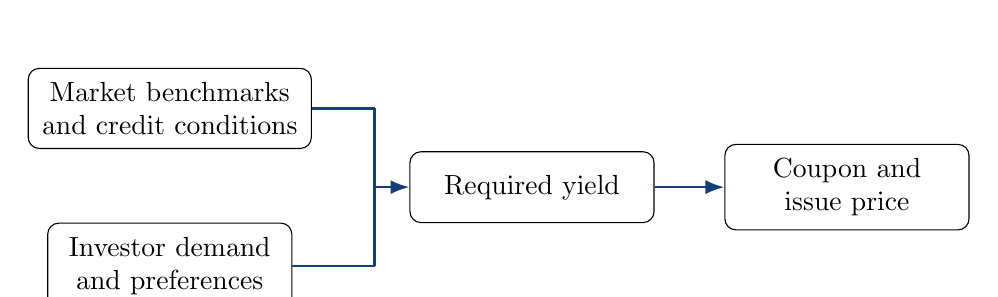
\begin{tikzpicture}[
  >=Latex,
  box/.style={
    draw,
    rounded corners,
    align=center,
    minimum width=3.1cm,
    minimum height=0.9cm,
    inner sep=5pt
  },
  flow/.style={-Latex, line width=0.85pt, FinanceBlue}
]

\node[box] (bench) at (-4.6,1.25)
{Market benchmarks\\and credit conditions};

\node[box] (demand) at (-4.6,-0.75)
{Investor demand\\and preferences};

\node[box] (yield) at (0,0.25)
{Required yield};

\node[box] (terms) at (4.0,0.25)
{Coupon and\\issue price};

% Two inputs converge into a common vertical line
\coordinate (mergeTop) at (-2.0,1.25);
\coordinate (mergeBottom) at (-2.0,-0.75);
\coordinate (mergeCenter) at (-2.0,0.25);

\draw[line width=0.85pt, FinanceBlue] (bench.east) -- (mergeTop);
\draw[line width=0.85pt, FinanceBlue] (demand.east) -- (mergeBottom);

% Shared connection and output
\draw[line width=0.85pt, FinanceBlue]
  (mergeTop) -- (mergeBottom);

\draw[flow] (mergeCenter) -- (yield.west);
\draw[flow] (yield.east) -- (terms.west);
\end{tikzpicture}

\caption{Pricing a new bond issue}

\label{fig:ch13-bond-issue-pricing}

\end{figure}

\subsection{Bookbuilding, Pricing, and Investor Allocation}

Bookbuilding is a process through which underwriters collect indications of investor demand before final pricing and allocation. Investors may indicate the quantities they are willing to purchase at different prices or yields, allowing the underwriters to assess both the strength and the distribution of demand.

Let $q_i(p)$ denote investor $i$'s indicated demand at price $p$. Aggregate indicated demand is

\begin{equation}
Q(p)=\sum_{i=1}^{n} q_i(p).
\label{eq:ch13-bookbuilding-demand}
\end{equation}

The order book provides more information than aggregate demand alone. Underwriters can observe the size and price sensitivity of orders, the composition of participating investors, and how demand changes as proposed terms are revised. This information helps assess the price at which the issue can be placed and the degree of uncertainty surrounding that demand.

Final pricing therefore uses the order book without following a purely mechanical rule. A more issuer-favorable price may increase proceeds per security but leave less room for changes in demand before the transaction is completed. Issuers and underwriters may also consider execution risk, investor participation, and expected secondary-market conditions when setting the final terms.

Allocation determines how the securities are distributed when indicated demand differs from the amount offered. Some offerings may use largely proportional allocations, while others allow greater discretion. Allocations can reflect order size, price sensitivity, investor characteristics, and the information conveyed during bookbuilding. Such discretion can improve the placement process, but it can also create conflicts when allocation decisions are influenced by relationships or objectives unrelated to the transaction.

\begin{example}{Price Sensitivity in Bond Bookbuilding}{bond-bookbuilding-sensitivity}

A company plans to issue RMB~1 billion in five-year bonds. During
bookbuilding, investors submit orders totaling RMB~1.6 billion
at an indicative yield of 3.0\%. However, RMB~500 million of
these orders are conditional on a yield of at least 3.2\%.

If the final yield is set at 3.0\%, these price-sensitive orders
may not participate, leaving only RMB~1.1 billion in orders
consistent with the final pricing terms. Even these orders may
be revised before allocation as market conditions change.

The underwriter must therefore assess not only the total volume
of submitted orders but also their price sensitivity and
reliability. Setting a higher yield may attract additional
demand, but it also increases the issuer's borrowing cost.
Bookbuilding thus involves balancing investor demand against
the financing cost faced by the issuer.
\end{example}

\section[Market Making and Secondary-Market Intermediation]{Market Making and Secondary-Market \\Intermediation}

In secondary markets, dealers support trading by quoting prices, executing client orders, and temporarily holding securities when buy and sell orders do not coincide. This activity uses balance-sheet capacity to absorb short-term inventory imbalances and facilitate transactions in marketable securities.

\subsection{Dealer Inventories, Balance Sheets, and Liquidity Provision}

A dealer can buy a security from a client before finding another investor willing to purchase it. The position enters dealer inventory, allowing the client to trade without waiting for an offsetting order.

Let $I_t$ denote the dealer's inventory at the end of period $t$, $Q_t^{B}$ purchases from clients, and $Q_t^{S}$ sales to clients. A simple inventory relation is

\begin{equation}
I_t=I_{t-1}+Q_t^{B}-Q_t^{S}.
\label{eq:ch13-dealer-inventory}
\end{equation}

Holding inventory exposes the dealer to price movements and requires funding and balance-sheet capacity. If a dealer buys bonds from clients and market yields rise before the position is sold, the value of the inventory can decline. Capital requirements, funding costs, hedging costs, and internal risk limits can therefore affect the willingness of dealers to absorb client orders.

\begin{example}{Inventory Risk in a Client Trade}{dealer-inventory-risk}

A dealer purchases a bond position with a market value of RMB~50 million and plans to resell it later in the day. If the market value falls by 0.4\%  before the position is sold, the mark-to-market loss is approximately

\[
50{,}000{,}000\times 0.004=\text{RMB }200{,}000.
\]

\end{example}

Dealer liquidity provision can therefore vary with market conditions. When volatility rises, funding becomes more costly, or risk limits become more restrictive, dealers may hold less inventory or quote less aggressively. Liquidity can weaken even when the contractual terms of the securities have not changed.

This inventory-bearing role distinguishes dealer intermediation from simple order matching. A trading platform can connect buyers and sellers without taking positions, whereas a dealer can provide immediacy by temporarily using its own balance sheet.

\subsection[Bid--Ask Spreads, Information, and Trading Costs]
{Bid--Ask Spreads, Information, and Trading \\Costs}

A dealer typically quotes a bid price at which it is willing to buy and an ask price at which it is willing to sell. The quoted spread is

\begin{equation}
s=P_{\mathrm{ask}}-P_{\mathrm{bid}}.
\label{eq:ch13-dealer-spread}
\end{equation}

The spread reflects several sources of trading cost and risk. Order processing and market access involve direct costs, while inventory positions expose the dealer to price and funding risk. Adverse selection adds an information component when the dealer may trade with investors who possess better information about the security's value.

The size of these components varies across securities and trades. A small transaction in a liquid security may require little inventory commitment, whereas a large trade in a less liquid security may be more difficult to offset and expose the dealer to greater price risk.

\begin{tcolorbox}[
  enhanced,
  breakable,
  colback=white,
  colframe=FinanceBlue,
  boxrule=0.7pt,
  sharp corners,
  borderline west={2.2pt}{0pt}{FinanceBlue},
  title=\textbf{Financial Perspective: The Quoted Spread Is Not the Entire Trading Cost},
  coltitle=white,
  colbacktitle=FinanceBlue,
  fonttitle=\bfseries,
  before skip=1.2em,
  after skip=1.2em
]

The quoted bid--ask spread describes the prices available for a stated quantity. A larger trade may require execution at less favorable prices if the quantity available at the best quotes is limited.

Trading cost can therefore include both the quoted spread and the additional price concession required to execute the desired quantity. This distinction becomes more important when trade size is large relative to available market liquidity.

\end{tcolorbox}

Information asymmetry can further affect dealer quotes. If incoming orders are more likely to contain information about future value, trading against those orders can generate losses for the dealer. Wider spreads, smaller quoted quantities, or less aggressive prices can reduce this exposure, although they also increase the cost of immediate execution for other investors.

Bid--ask spreads therefore reflect the cost of providing immediacy under uncertainty. They tend to depend on the liquidity of the security, the size of the trade, the dealer's risk exposure, and the information environment in which the transaction occurs.

\section{Advisory and Strategic Transactions}

Investment banks also advise firms on transactions that alter ownership, control, or capital structure. Their role is to help evaluate alternatives, negotiate terms, arrange financing when needed, and coordinate the execution of transactions whose value depends on firm-specific information and contractual design.

\subsection{Mergers and Acquisitions Advisory}

Mergers and acquisitions transfer or reorganize control over corporate assets and cash flows. Investment banks may advise buyers, sellers, targets, or special committees by assessing transaction alternatives, estimating value, identifying counterparties, and supporting negotiation and execution.

Transaction decisions involve more than valuation alone. A buyer may expect operating or financial benefits from combining two firms but face uncertainty about whether those gains can be realized. A seller may consider not only price but also the form of consideration, financing certainty, regulatory approval, and the probability that the transaction will be completed. Valuation therefore provides a basis for negotiation rather than a uniquely determined transaction price.

A simple framework separates stand-alone value from the incremental value expected from the combination. Let $V_{acquirer}$ and $V_{target}$ denote the stand-alone values of the acquirer and target, $S$ the expected gross gains from combining them, and $C$ the present value of transaction and integration costs. The combined value is

\begin{equation}
V_{merger}=V_{acquirer}+V_{target}+S-C.
\label{eq:ch13-combined-transaction-value}
\end{equation}

If the acquirer pays total consideration $P_{target}$ for the target, the expected NPV to the acquirer's existing shareholders in this simplified framework is

\begin{equation}
\textit{NPV}_{acquirer}=S-C-(P_{target}-V_{target}).
\label{eq:ch13-acquirer-transaction-npv}
\end{equation}

The term $P_{target}-V_{target}$ is the acquisition premium relative to the target's estimated stand-alone value. A transaction may generate positive combined gains while allocating a substantial share of those gains to target shareholders through the negotiated premium.

\begin{example}{Synergy and the Negotiated Premium}{ma-synergy-premium}

A target has an estimated stand-alone value of RMB~1.0 billion. A buyer expects gross combination benefits of RMB~250 million and integration costs with a present value of RMB~50 million. The expected net incremental value is therefore RMB~200 million.

If the agreed purchase price is RMB~1.15 billion, the premium over the target's estimated stand-alone value is RMB~150 million. Under these assumptions, the buyer's expected transaction NPV is

\[
200-150=\text{RMB }50\text{ million}.
\]

\end{example}

The adviser helps the client evaluate these trade-offs and translate valuation estimates into transaction terms. Advisory work can improve the quality and execution of the decision, but it does not establish that the transaction will ultimately create value.

\subsection{Restructuring, Recapitalization, and Distressed Transactions}

Firms may alter their capital structures for strategic reasons or in response to financial pressure. A recapitalization changes the mix, maturity, or ownership structure of financial claims without necessarily altering the firm's operating assets. When payment obligations become difficult to sustain, restructuring may require more substantial changes to debt terms, priority, recovery, or control.

Investment banks may advise the company, creditors, or investors in evaluating these alternatives. In a recapitalization, the analysis may focus on leverage, maturity structure, financing flexibility, and the allocation of ownership and control. Under financial distress, greater attention shifts to enterprise value, expected recovery, near-term financing needs, and the distribution of value across claimant groups. Possible transactions include debt or equity issuance, maturity extensions, exchange offers, new financing, and asset sales.

A liability-management transaction illustrates the mechanism. A firm facing near-term maturities may offer longer-dated securities in exchange for existing debt. Extending maturity can reduce immediate refinancing pressure, but creditors will compare the value, priority, collateral, and expected recovery of the new claims with those of the securities they surrender. The terms must therefore provide sufficient value for enough holders to participate.

Distressed transactions can also redistribute value and control among claimant classes. Senior creditors, junior creditors, and shareholders may have different preferences over recovery, risk, and future control of the firm. Advisers can support valuation, transaction design, and negotiation, while the enforceable rights of each claimant remain governed by contracts and applicable law.

\subsection{Valuation, Negotiation, and Transaction Execution}

Valuation provides a framework for comparing transaction alternatives, but it typically depends on assumptions rather than producing a uniquely determined value. Discounted cash-flow analysis depends on forecasts and discount rates, while comparable-company and precedent-transaction methods depend on the relevance of the selected benchmarks. Strategic value may also differ across buyers when expected synergies, financing capacity, or control benefits differ. Investment banks therefore often use valuation ranges and sensitivity analysis to show how estimated value changes with key assumptions.

Negotiation converts these valuation assessments into transaction terms. Price is only one dimension. Consideration may take the form of cash, shares, debt, or a combination, while earn-outs, contingent payments, break fees, financing conditions, and closing provisions can alter the allocation of risk and value. Transactions with similar headline prices can therefore create different economic exposures for the parties involved.

Execution determines whether the negotiated transaction is completed on the agreed terms. Advisers coordinate financing, documentation, timetables, and information flows across legal, accounting, regulatory, and other work streams. Changes in financing conditions, regulatory review, shareholder approval, due diligence findings, or market conditions can affect both the probability and the terms of completion.

\begin{tcolorbox}[
  enhanced,
  breakable,
  colback=white,
  colframe=FinanceBlue,
  boxrule=0.7pt,
  sharp corners,
  borderline west={2.2pt}{0pt}{FinanceBlue},
  title=\textbf{Financial Perspective: Value and Price Are Not the Same},
  coltitle=white,
  colbacktitle=FinanceBlue,
  fonttitle=\bfseries,
  before skip=1.2em,
  after skip=1.2em
]

Valuation estimates the economic value of a transaction under stated assumptions. The negotiated price reflects not only those estimates but also bargaining conditions, competing offers, financing terms, contractual protections, and execution risk.

A valuation range therefore informs negotiation without mechanically determining the final transaction price.

\end{tcolorbox}

%========================================================
% Summary
%========================================================

\TailModule{summary}{Summary}

Investment banks support capital-market transactions through information production, certification, security design, distribution, and execution. Their role differs from traditional balance-sheet intermediation because investors generally continue to hold claims issued directly by the financing entity.

Underwriting helps move securities from issuers to investors. Firm commitments expose underwriters to placement risk, syndication shares distribution capacity and exposure, and bookbuilding provides information for pricing and allocation.

In secondary markets, dealers use inventory and balance-sheet capacity to provide immediacy. Bid--ask spreads reflect transaction costs, inventory exposure, information risk, and prevailing market conditions.

Investment banks also advise on mergers, acquisitions, recapitalizations, and restructurings. Across these activities, their economic role rests on information, reputation, valuation, transaction expertise, and selective use of balance-sheet capacity.

%========================================================
% Key Terms
%========================================================

\TailModule{keyterms}{Key Terms}

Investment bank; capital-market intermediation; certification; due diligence; security design; underwriting; best efforts; underwriting spread; underwriting syndicate; initial public offering; primary shares; secondary shares; debt underwriting; bookbuilding; indication of interest; investor allocation; market making; dealer inventory; bid--ask spread; strategic advisory; merger; acquisition; acquisition premium; recapitalization; restructuring; liability management; transaction execution.

%========================================================
% Financial AI Lab
%========================================================

\TailModule{aiprompt}{Financial AI Lab}

\textbf{Lab: Audit an AI Capital-Raising Recommendation}

Select a publicly listed company that has recently raised equity or debt capital. Ask an AI system to act as an investment-bank adviser and recommend an issuance structure. The recommendation should identify the financing objective, security type, issue size, likely investor base, relevant valuation or yield benchmarks, and major execution risks.

Audit the recommendation in four stages.

\begin{enumerate}

\item \textbf{Verify the financing need and existing capital structure.}

Use financial statements and formal disclosures to confirm the firm's debt, equity, liquidity position, and stated use of proceeds. Separate verified facts from assumptions introduced by the AI.

\item \textbf{Evaluate security design.}

Assess whether the proposed security terms fit the issuer's financing needs and the likely investor base. For debt, consider maturity, payment structure, seniority, and collateral where relevant. For equity, consider issue size, ownership effects, and the form of the offering. Identify one alternative structure and explain the main trade-off.

\item \textbf{Audit pricing evidence.}

For an equity issue, compare the proposed valuation with observable market prices or suitable comparable-company evidence. For a bond issue, compare the proposed yield or spread with an appropriate benchmark curve and comparable issuers. Check that dates, currencies, maturities, and units are consistent.

\item \textbf{Separate advice from underwriting commitment.}

Identify which parts of the recommendation concern information, valuation, and transaction advice and which would expose the investment bank to underwriting risk. Explain how the distribution risk changes under a firm commitment relative to a placement or best-efforts arrangement.

\end{enumerate}

%========================================================
% Discussion Questions
%========================================================

\TailModule{questions}{Discussion Questions}
\begin{enumerate}

\item Why does using an investment bank in a securities offering not, by itself, convert direct finance into indirect finance?

\item How can investment-bank reputation reduce information frictions, and why does certification not eliminate the need for investor judgment?

\item What distribution risk does a firm-commitment underwriter assume that a best-efforts intermediary generally does not?

\item Why can the final offer price in a bookbuilt transaction differ from the highest price indicated by some investor orders?

\item How does dealer inventory support liquidity provision, and what balance-sheet risks does the dealer assume?

\item In an acquisition, why can target shareholders receive substantial gains even when little value remains for the acquirer's existing shareholders?

\end{enumerate}

%========================================================
% Applied Problems
%========================================================

\TailModule{appprobs}{Applied Problems}

\begin{enumerate}

\item \textbf{Underwriting economics.}

A company issues 30 million shares in a firm-commitment offering at a public price of RMB~18 per share. The underwriting group purchases the shares from the issuer at RMB~17.55 per share.

\begin{enumerate}
\item Calculate the gross underwriting spread per share.
\item Calculate the total gross spread.
\item Calculate the proceeds received by the issuer before other offering expenses.
\item Explain why the gross spread is not the same as the underwriting group's profit.
\end{enumerate}

\item \textbf{Primary and secondary shares.}

An IPO contains 80 million primary shares issued by the company and 20 million secondary shares sold by existing shareholders. The offer price is RMB~12 per share.

\begin{enumerate}
\item Calculate the gross proceeds associated with the primary shares.
\item Calculate the gross proceeds associated with the secondary shares.
\item Which amount enters the company before fees and expenses?
\item Explain how the two components affect ownership and financing differently.
\end{enumerate}

\item \textbf{Bookbuilding and demand.}

An issuer plans to sell 50 million shares. Indications of demand are 90 million shares at RMB~20, 65 million at RMB~21, and 42 million at RMB~22.

\begin{enumerate}
\item At which of the stated prices does indicated demand exceed the amount offered?
\item Why is this information insufficient by itself to identify a unique offer price?
\item Identify two qualitative features of the order book that an underwriter may examine in addition to aggregate quantity.
\item Explain how a higher offer price can affect both issuer proceeds and execution risk.
\end{enumerate}

\item \textbf{Dealer inventory.}

A dealer begins the day with a bond position with a market value of RMB~10 million. It purchases bonds with a market value of RMB~35 million from clients and sells RMB~28 million during the day.

\begin{enumerate}

\item Calculate the ending inventory, measured at the stated transaction values.

\item If the ending inventory subsequently falls in value by 0.6\%  before it is sold, calculate the mark-to-market loss.

\item Identify two additional costs that may affect the economics of providing liquidity.

\item Explain how tighter internal risk limits could affect client execution even if the bond's contractual cash flows are unchanged.

\end{enumerate}

\item \textbf{Acquisition value and negotiation.}

A target has an estimated stand-alone value of RMB~2.0 billion. A bidder estimates gross synergies of RMB~420 million and integration and transaction costs with present value of RMB~120 million.

\begin{enumerate}
\item Calculate estimated net incremental value.
\item If the bidder offers RMB~2.24 billion, calculate the premium over stand-alone value.
\item Using Equation~(\ref{eq:ch13-acquirer-transaction-npv}), calculate the bidder's expected transaction NPV under the stated assumptions.
\item Recalculate the NPV if integration costs rise to RMB~220 million.
\item Explain why the negotiated price may differ from a valuation estimate based on these assumptions.
\end{enumerate}

\item \textbf{Bond issuance and market feedback.}

A company plans to issue a five-year bond. The five-year government yield is 3.0\% . Comparable corporate bonds trade at spreads of about 110 basis points over the government benchmark. Initial investor feedback suggests weak demand at a spread of 100 basis points but stronger demand near 120 basis points.

\begin{enumerate}

\item Calculate the benchmark yield implied by a spread of 110 basis points.

\item Calculate the issue yield implied by a spread of 120 basis points.

\item Explain why the issuer may accept the higher spread even though it increases borrowing cost.

\item Identify two factors, other than the benchmark yield, that could cause the final issue terms to change before placement.

\end{enumerate}

\end{enumerate}

%========================================================
% Case Analysis
%========================================================

\TailModule{caseanalysis}{Case Analysis}

\CaseLabel{Historical Case Based on Public Information}

\textbf{Case: Alibaba's 2014 U.S. Initial Public Offering}

Alibaba Group Holding Limited priced its U.S. initial public offering in September 2014 at US\$68 per American depositary share (ADS). The base offering included 320,106,100 ADSs: Alibaba offered 123,076,931 newly issued ADSs, while existing shareholders offered 197,029,169 ADSs. At the offer price, the gross proceeds of the base offering were approximately US\$21.77 billion.\footnote{Alibaba Group Holding Limited, final prospectus filed with the U.S. Securities and Exchange Commission, September 2014.}

Six investment banks acted as joint bookrunners. The prospectus reported underwriting discounts and commissions of US\$0.816 per ADS. Alibaba and certain selling shareholders also granted the underwriters an option to purchase up to 48,015,900 additional ADSs. The option was subsequently exercised in full, increasing total gross proceeds to approximately US\$25.03 billion.

Use the transaction to examine several investment-banking functions. First, distinguish the primary ADSs sold by Alibaba from the secondary ADSs sold by existing shareholders. Which portion raised new capital for the company, and which portion transferred ownership from existing shareholders to new investors?

Second, calculate the underwriting discount as a percentage of the US\$68 offer price. What services and risks does this compensation reflect, and why should it not be interpreted as pure underwriting profit?

Third, consider the role of the joint bookrunners. How can a syndicate broaden investor coverage, aggregate information during bookbuilding, and share distribution exposure? What tension can arise between the issuer's interest in a higher offer price and the underwriters' concerns about execution risk and investor participation?

Finally, explain how the option to purchase additional ADSs can provide flexibility beyond the base offering size and support the distribution process. Keep the analysis focused on underwriting and distribution rather than on subsequent share-price performance.

\emph{Primary sources: Alibaba Group Holding Limited, final prospectus filed with the U.S. Securities and Exchange Commission, September 2014; Alibaba Group announcements on IPO pricing and the exercise of the underwriters' option, September 2014.}

%========================================================
% Further Reading
%========================================================

\TailModule{furtherread}{Further Reading}

\begin{itemize}

\item Beatty, Randolph P., and Jay R. Ritter (1986),
``Investment Banking, Reputation, and the Underpricing of Initial Public Offerings,''
\emph{Journal of Financial Economics}, 15(1--2), 213--232.

\item Benveniste, Lawrence M., and Paul A. Spindt (1989),
``How Investment Bankers Determine the Offer Price and Allocation of New Issues,''
\emph{Journal of Financial Economics}, 24(2), 343--361.

\item Chemmanur, Thomas J., and Paolo Fulghieri (1994),
``Investment Bank Reputation, Information Production, and Financial Intermediation,''
\emph{The Journal of Finance}, 49(1), 57--79.

\item Ellis, Katrina, Roni Michaely, and Maureen O'Hara (2000),
``When the Underwriter Is the Market Maker: An Examination of Trading in the IPO Aftermarket,''
\emph{The Journal of Finance}, 55(3), 1039--1074.

\item Servaes, Henri, and Marc Zenner (1996),
``The Role of Investment Banks in Acquisitions,''
\emph{The Review of Financial Studies}, 9(3), 787--815.

\end{itemize}

\ChapterTail{summary,keyterms,aiprompt,questions,appprobs,caseanalysis,furtherread}

\chapter{Asset Management and Institutional Investment}
\label{chap:Asset_Management_and_Institutional_Investment}

\begin{openingcase}{Whose Interests Does the Manager Serve?}

A pension fund invests retirement savings on behalf of thousands of beneficiaries. The beneficiaries ultimately bear the investment gains and losses, but they do not select individual securities or trade the portfolio themselves. Instead, the fund delegates much of this responsibility to professional asset managers.

One manager identifies an investment opportunity that would require a substantial departure from the benchmark and may take several years to pay off. If the investment succeeds, the gains accrue largely to the pension beneficiaries. If it underperforms the benchmark in the short run, however, the pension fund may reduce or terminate the mandate, cutting the manager's fee income. The manager may therefore hesitate to take a position that is consistent with the beneficiaries' long-term interests but exposes the mandate to short-term performance risk.

\end{openingcase}


\begin{tcolorbox}[
  enhanced,
  colback=FinanceBlue!6,
  colframe=FinanceBlue,
  boxrule=0.6pt,
  sharp corners,
  left=8pt,
  right=8pt,
  top=7pt,
  bottom=7pt,
  before skip=1em,
  after skip=1.6em,
  title=\textbf{Core Questions},
  coltitle=white,
  colbacktitle=FinanceBlue,
  fonttitle=\bfseries,
  attach boxed title to top left={xshift=6pt,yshift=-2mm},
  boxed title style={
    boxrule=0pt,
    sharp corners,
    left=5pt,
    right=5pt,
    top=2pt,
    bottom=2pt
  }
]
\begin{enumerate}[
  leftmargin=*,
  label=\textcolor{FinanceBlue}{\textbf{\arabic*.}},
  itemsep=0.55em,
  topsep=0.2em
]


\item Why do investors delegate portfolio decisions, and how do mandates, benchmarks, fees, and fiduciary responsibilities affect the relationship between investors and asset managers?

\item How do different asset-management vehicles and institutional investors differ in liquidity, control, investment horizon, and risk allocation?

\item How do asset managers produce information, affect markets and corporate governance, and respond to passive and technology-driven investment?


\end{enumerate}
\end{tcolorbox}

\section{The Economics of Delegated Asset Management}

Asset management separates capital ownership from many investment decisions. Investors bear the portfolio's gains and losses, while professional managers receive authority to select, trade, monitor, and sometimes vote the securities within a defined mandate.

\subsection{Direct and Delegated Investment}

An individual investor can hold and manage financial assets directly or delegate portfolio decisions to a professional manager. Direct investment gives the investor control over security selection, trading, and portfolio monitoring, but also requires time, information, and investment expertise. Under delegated investment, the investor retains the economic exposure to the portfolio, while the manager receives authority to make specified investment decisions within a defined mandate. The precise legal arrangement depends on whether the assets are held through a pooled vehicle, a separate account, or another structure.

Delegation can create value when portfolio management requires expertise, scale, or infrastructure that is costly for individual investors to reproduce. Managers can spread the costs of research, trading systems, risk measurement, reporting, and administration across many clients. Pooled investment vehicles can also provide diversification at lower transaction and monitoring costs than many investors could achieve individually.

This structure differs from deposit-taking intermediation. A commercial bank finances much of its asset portfolio by issuing deposits and other liabilities on its own balance sheet. An asset manager, by contrast, typically manages client assets or pooled funds without financing those assets primarily with its own liabilities. Portfolio gains and losses are therefore generally passed through to investors, subject to the legal structure of the vehicle and any contractual commitments or capital provided by the manager.

A simple delegated-investment relationship can be written as

\begin{equation}
W_T=W_0(1+r_{gross})-F,
\label{eq:ch14-investor-terminal-wealth}
\end{equation}
where $W_0$ is the investor's initial capital, $r_{gross}$ is the
gross portfolio return over the period, and $F$ represents
the total fees and other charges, expressed as a monetary
amount. Compared with direct investment, delegation changes who makes portfolio decisions and introduces management costs, while the investor generally remains exposed to portfolio performance.

\subsection{Asset Management Contracts, Fees, and Incentives}

Delegated asset management is governed by contracts that define decision rights, investment constraints, and compensation. An investment mandate may specify eligible assets, benchmarks, risk limits, leverage, investment horizon, and reporting requirements. In pooled vehicles, fund terms may also govern liquidity and withdrawals. Together, these provisions define the manager's decision space and the basis for performance evaluation.

A benchmark provides a reference portfolio or return against which portfolio performance can be assessed. If $r_P$ is the portfolio return and $r_B$ the benchmark return, active return is

\begin{equation}
r_{active}=r_P-r_B.
\label{eq:ch14-active-return}
\end{equation}

Benchmarking makes relative performance and portfolio deviations more visible, but it can also affect investment decisions. A manager evaluated closely against a benchmark may limit large deviations that could generate substantial relative underperformance.

Compensation commonly includes an asset-based management fee. If the annual fee rate is $f$ and $A$ is the relevant fee base, the management fee can be written as

\begin{equation}
F_M=fA.
\label{eq:ch14-management-fee}
\end{equation}

Some arrangements also include performance-based compensation. A performance fee can be expressed as

\begin{equation}
F_P=\alpha\max\{r_P-h,0\}A,
\label{eq:ch14-performance-fee}
\end{equation}
where $\alpha$ is the performance-fee rate, $h$ is a hurdle or reference return, and $A$ is the fee base. More detailed contracts may include high-water marks, loss carryforwards, or benchmark adjustments.

Fee design affects managerial incentives. Asset-based fees link revenue to assets under management and can increase the value of attracting and retaining investor capital. Performance fees make compensation more sensitive to investment outcomes, but asymmetric participation in gains and losses may encourage greater risk taking under some conditions. The resulting incentives depend on the contract as a whole and on any capital that the manager has invested alongside clients.

\begin{example}{Management Fees and Net Investor Return}{management-fee-net-return}

A fund begins the year with RMB~100 million and earns a gross portfolio return of 8\%. Suppose the management fee is 1\% of beginning assets and there are no other fees or cash flows.

The management fee is

\[
F_M=0.01\times100=1
\]

million RMB. Portfolio gains increase the fund's assets to RMB~108 million before fees. After the management fee is deducted, net assets are RMB~107 million, corresponding to a simplified net return of 7\%.

The one-percentage-point difference between gross and net return reflects the management fee under the stated convention.

\end{example}

\subsection[principal-agent Problems and Fiduciary Responsibility]{principal-agent Problems and Fiduciary \\Responsibility}

Delegated asset management creates a principal-agent relationship. Investors entrust investment authority to managers, but managerial objectives may not always coincide fully with investor interests. Compensation, career concerns, asset gathering, and business relationships can influence how that authority is exercised.

Agency conflicts can take several forms. Managers may assume additional risk when compensation is asymmetric, remain close to a benchmark to reduce career risk, trade more than investment considerations justify, or favor affiliated products or counterparties. Such outcomes are not inherent in delegation; their importance depends on contract design, organizational structure, and the regulatory environment.

Fiduciary responsibility constrains the use of delegated authority. Its legal content varies across jurisdictions and institutional forms, but the underlying economic principle is that managers should exercise entrusted authority with due regard to client interests and manage conflicts of interest appropriately. Disclosure, internal controls, independent oversight, and restrictions on conflicted transactions can support this objective.

Investors can also discipline managers through monitoring and exit. Institutional clients may negotiate mandates, review performance, and replace managers, while retail investors rely more heavily on standardized disclosure, fund governance, regulation, and the ability to redeem or switch funds. Reputation provides an additional constraint when future mandates and asset flows depend on investor confidence.

\begin{tcolorbox}[
  enhanced,
  breakable,
  colback=white,
  colframe=FinanceBlue,
  boxrule=0.7pt,
  sharp corners,
  borderline west={2.2pt}{0pt}{FinanceBlue},
  title=\textbf{Financial Perspective: Fiduciary Responsibility Does Not Eliminate Agency Problems},
  coltitle=white,
  colbacktitle=FinanceBlue,
  fonttitle=\bfseries,
  before skip=1.2em,
  after skip=1.2em
]

Fiduciary responsibility constrains how managers use delegated authority, but it does not make investor and manager incentives identical. Investment outcomes are uncertain, managerial actions are not always fully observable, and conflicts of interest may remain. Contracts, monitoring, governance, and reputation therefore continue to matter even when fiduciary obligations apply.

\end{tcolorbox}

\section{Collective Investment Vehicles}

One common way to organize delegated investment is through a collective investment vehicle. Instead of managing each investor's portfolio separately, the vehicle pools capital from many investors and invests the combined resources under a common mandate.

\subsection{Open-End Mutual Funds}

An open-end mutual fund issues shares that investors can subscribe to or redeem with the fund. Subscriptions create new shares, while redemptions cancel existing shares, so the number of shares outstanding changes with investor flows.

The net asset value (NAV) per share is

\begin{equation}
\textit{NAV}_t=
\frac{A_t-L_t}{N_t},
\label{eq:ch14-nav}
\end{equation}

where $A_t$ is the market value of fund assets, $L_t$ is fund liabilities, and $N_t$ is the number of shares outstanding. NAV converts the net value of the fund's portfolio into a value per share.

Investor flows can affect portfolio management. Subscriptions provide cash that may be invested in additional assets, while redemptions require the fund to provide cash to departing investors. The fund can meet redemptions from cash holdings, offsetting subscriptions, permitted borrowing, or asset sales. When redemptions are large relative to available liquidity, the manager may need to sell assets even when the underlying investment view has not changed.

Open-end pooling can provide diversification and economies in trading and administration, but it also creates a link between investor liquidity and portfolio liquidity. The cost of meeting redemptions therefore depends partly on how readily the underlying assets can be sold.

\begin{example}{A Mutual Fund Subscription at NAV}{mutual-fund-subscription-nav}

A mutual fund has RMB~500 million of assets, RMB~5 million of liabilities, and 45 million shares outstanding. Its NAV per share is

\[
\textit{NAV}=\frac{500-5}{45}=11.00.
\]

An investor contributes RMB~1.1 million at this NAV and, abstracting from fees, receives

\[
\frac{1.1\text{ million}}{11.00}=100{,}000
\]

new fund shares. The subscription increases fund assets to RMB~501.1 million and shares outstanding to 45.1 million. Under the stated assumptions, NAV remains RMB~11.00 per share.

\end{example}

\subsection[Exchange-Traded Funds and the Creation--Redemption Mechanism]{Exchange-Traded Funds and the Creation--\\Redemption Mechanism}

An exchange-traded fund (ETF) holds a portfolio of underlying assets while its shares trade in the secondary market. Most investors buy and sell ETF shares without transacting directly with the fund. Authorized participants, however, can create or redeem large blocks of shares through transactions with the fund.

In a creation, an authorized participant delivers a specified basket of securities, cash, or a combination of the two and receives newly issued ETF shares. In a redemption, ETF shares are returned to the fund in exchange for a corresponding basket or cash settlement. This mechanism allows the supply of ETF shares to adjust in response to conditions in the ETF and its underlying portfolio.

Let $P_t^{ETF}$ denote the market price of an ETF share and $\textit{NAV}_t$ its net asset value per share. The ETF premium or discount relative to NAV can be measured as

\begin{equation}
\pi_t=
\frac{P_t^{ETF}-\textit{NAV}_t}{\textit{NAV}_t}.
\label{eq:ch14-etf-premium-discount}
\end{equation}

When an ETF trades at a sufficiently large premium, authorized participants can create new shares and sell them in the secondary market, tending to reduce the premium. When it trades at a sufficiently large discount, redemption can work in the opposite direction. The effectiveness of this mechanism depends on transaction costs, funding conditions, taxes, market hours, and the liquidity of the underlying assets.

\begin{example}{ETF Creation When the Fund Trades at a Premium}{etf-creation-premium}

Suppose an ETF has a NAV of RMB~10.00 per share but trades in the secondary market at RMB~10.10. Ignoring transaction costs and other frictions, an authorized participant can acquire the underlying basket at a value equivalent to RMB~10.00 per ETF share, deliver the basket to the fund, and receive newly created ETF shares.

If those shares are then sold at RMB~10.10, the price difference creates an arbitrage opportunity. The creation increases the supply of ETF shares and tends to reduce the premium.

In practice, creation becomes attractive only when the price difference is large enough to cover transaction costs, funding costs, taxes, and other frictions.

\end{example}

Unlike an ordinary open-end mutual fund, an ETF does not require the fund itself to transact whenever an investor buys or sells shares. Secondary-market trading can therefore absorb many investor transactions without directly changing the underlying portfolio. Creation and redemption nevertheless provide a channel through which trading pressure can pass between ETF shares and the underlying assets.

\subsection{Fund Liquidity, NAV, and Redemption Risk}

The liquidity of a fund claim and the liquidity of its underlying assets are related but distinct. A fund may offer frequent subscriptions and redemptions even when some portfolio assets trade less frequently. This arrangement is easier to maintain when investor flows are small relative to available cash and market liquidity.

Large redemptions can require asset sales. When portfolio assets are relatively illiquid, such sales may involve transaction costs, price concessions, or market impact. If these costs are not fully reflected in the price received by redeeming investors, part of the cost may be borne by investors who remain in the fund. Under such conditions, expectations of further outflows can create an incentive to redeem earlier.

Fund design can affect how these costs are distributed. Cash buffers and liquid holdings can reduce the need for immediate asset sales, while redemption fees, swing pricing, notice periods, and other liquidity-management tools can shift more of the cost toward investors whose transactions generate it. Their use depends on the structure of the fund, the liquidity of its assets, and applicable rules.

Illiquid assets can also complicate NAV measurement. When market prices are unavailable or infrequent, valuation may rely more heavily on models, dealer quotations, comparable securities, or other estimation methods. NAV remains a useful measure of investor claims, but valuation uncertainty may increase when observable market prices provide less information.

\begin{figure}[H]
\centering
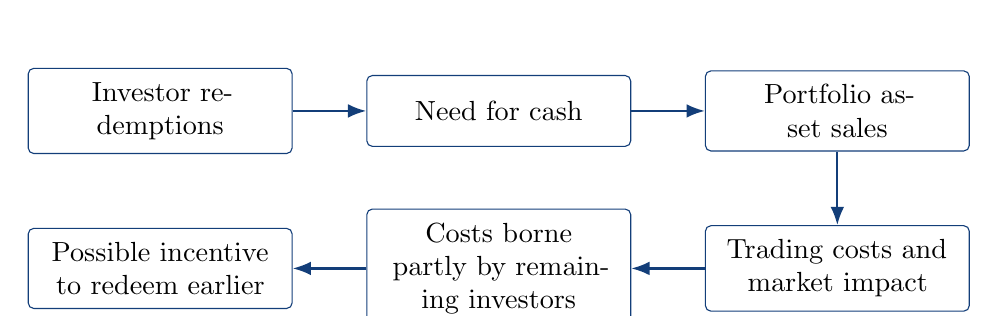
\begin{tikzpicture}[
  >=Latex,
  box/.style={
    draw=FinanceBlue,
    rounded corners=2pt,
    align=center,
    text width=3.0cm,
    minimum height=0.9cm,
    inner sep=5pt
  },
  flow/.style={-Latex, line width=0.8pt, FinanceBlue}
]

\node[box] (redeem) at (0,0) {Investor redemptions};
\node[box] (cash) at (4.3,0) {Need for cash};
\node[box] (sales) at (8.6,0) {Portfolio asset sales};

\node[box] (costs) at (8.6,-2.0) {Trading costs and market impact};
\node[box] (remain) at (4.3,-2.0) {Costs borne partly by remaining investors};
\node[box] (incentive) at (0,-2.0) {Possible incentive to redeem earlier};

\draw[flow] (redeem) -- (cash);
\draw[flow] (cash) -- (sales);
\draw[flow] (sales) -- (costs);
\draw[flow] (costs) -- (remain);
\draw[flow] (remain) -- (incentive);

\end{tikzpicture}
\caption{Redemption pressure and liquidity costs in an open-end fund}
\label{fig:ch14-redemption-liquidity}
\end{figure}

\section{Institutional Investors and Alternative Asset Management}

Beyond collective investment vehicles, delegated investment is also organized through institutions with different liability structures, investment horizons, liquidity needs, and governance arrangements. These characteristics influence the assets they can hold, the risks they can bear, and the way they interact with financial markets and corporate issuers.

\subsection{Pension Funds and Liability-Driven Investment}

Pension funds invest assets to meet future benefit obligations. Their asset strategy therefore depends on the timing, inflation sensitivity, and uncertainty of those payments as well as on expected asset returns.

Let expected pension payments be $B_t$ at dates $t=1,\ldots,T$. A simplified present value of liabilities is

\begin{equation}
L_0=\sum_{t=1}^{T}\frac{B_t}{(1+y_t)^t},
\label{eq:ch14-pension-liability-pv}
\end{equation}
where $y_t$ is the discount rate applied to the payment at date $t$. The funding ratio is

\begin{equation}
FR=\frac{A_0}{L_0},
\label{eq:ch14-pension-funding-ratio}
\end{equation}
where $A_0$ is the market value of pension assets.

Liability-driven investment (LDI) manages assets relative to the value and sensitivity of pension liabilities. Long-duration bonds, for example, can reduce the sensitivity of the funding position to interest-rate changes when their duration is closer to that of the liabilities. Other assets may be held to seek higher expected returns. The allocation depends on funding status, benefit design, contribution policy, regulatory constraints, and tolerance for funding volatility.

Long-dated liabilities can also give pension funds greater capacity to hold less liquid assets when near-term benefit payments and collateral needs remain manageable. A long investment horizon does not eliminate liquidity risk; it can broaden the feasible investment set when sufficient liquidity is available to meet shorter-term obligations.

\begin{tcolorbox}[
  enhanced,
  breakable,
  colback=white,
  colframe=FinanceBlue,
  boxrule=0.7pt,
  sharp corners,
  borderline west={2.2pt}{0pt}{FinanceBlue},
  title=\textbf{Financial Perspective: LDI Focuses on the Funding Position, Not Assets Alone},
  coltitle=white,
  colbacktitle=FinanceBlue,
  fonttitle=\bfseries,
  before skip=1.2em,
  after skip=1.2em
]

Liability-driven investment evaluates asset risk relative to pension liabilities. An asset portfolio can perform well in isolation while the funding position deteriorates if liabilities rise by more. The relevant question is therefore how asset values and liability values move together.

\end{tcolorbox}

\subsection{Sovereign Wealth Funds, Endowments, and Long-Horizon Capital}

Sovereign wealth funds, endowments, foundations, and similar institutions often invest over long horizons, but their sources of capital and spending obligations differ substantially. Sovereign funds may be financed by commodity revenues, fiscal surpluses, foreign-exchange reserves, or intergenerational saving, while endowments typically support recurring institutional expenditures and seek to preserve purchasing power over time.

These differences affect liquidity needs and asset allocation. A long investment horizon can increase the capacity to hold less liquid assets such as private equity, infrastructure, and real estate, provided that near-term cash requirements remain manageable. Horizon alone is therefore not sufficient; the institution must also have the liquidity and governance capacity to maintain long-term positions.



\begin{tcolorbox}[
  enhanced,
  breakable,
  colback=white,
  colframe=FinanceBlue,
  boxrule=0.7pt,
  sharp corners,
  borderline west={2.2pt}{0pt}{FinanceBlue},
  title=\textbf{Financial Perspective: A Long Horizon Does Not Eliminate Liquidity Constraints},
  coltitle=white,
  colbacktitle=FinanceBlue,
  fonttitle=\bfseries,
  before skip=1.2em,
  after skip=1.2em
]

A long investment horizon can increase an institution's capacity to hold less liquid assets, but horizon alone is not enough. Spending needs, possible withdrawals, collateral requirements, and governance constraints can still require access to cash. The ability to invest for the long term therefore depends on both investment horizon and liquidity capacity.

\end{tcolorbox}

Spending rules and institutional objectives further influence portfolio choice. An endowment with relatively stable annual distributions may place greater emphasis on long-run real returns, while a sovereign fund with stabilization objectives may hold more liquid assets if withdrawals are likely to rise during adverse economic conditions.

Long-horizon capital can also reduce the need for forced sales during temporary market stress. Institutions with sufficient liquidity may be able to maintain positions through short-run price declines when doing so remains consistent with their mandate and risk capacity.

\subsection{Private Equity and Venture Capital}

Private equity and venture capital commonly organize investment through closed-end funds in which limited partners commit capital and a general partner makes investment decisions. Investors generally cannot redeem their interests on demand, giving the fund greater capacity to hold illiquid investments over extended periods.

A central feature of private-market investing is concentrated ownership and active monitoring. Buyout funds may acquire substantial or controlling interests and influence financing, governance, management, and operating decisions. Venture-capital investors typically finance younger firms in stages and may combine capital with board participation and close monitoring. These arrangements can be especially important when information is limited and firm value depends heavily on future development.

Manager compensation commonly combines a management fee with a performance-linked share of investment gains, often referred to as carried interest. This gives the general partner a direct stake in investment outcomes while leaving room for incentive conflicts. Fund terms, distribution rules, and capital contributed by the manager can affect how gains, losses, and incentives are shared between general and limited partners.

Valuation is more difficult when portfolio companies are not continuously traded. Fund values may rely on models, comparable transactions, or other valuation methods between observable market transactions. Reported values may therefore adjust more gradually than public-market prices and contain greater estimation uncertainty.

\subsection{Hedge Funds and Alternative Investment Strategies}

Hedge funds often operate under relatively flexible investment mandates and may use short selling, derivatives, leverage, relative-value positions, event-driven strategies, or concentrated exposures. These tools allow managers to express both positive and negative views, hedge selected risks, and construct positions that are difficult to implement in traditional long-only portfolios.

Such strategies can introduce funding, margin, liquidity, and model risk in addition to the market risk of the underlying positions. Their risk therefore depends not only on the assets held but also on how positions are financed, combined, and collateralized.

Investor liquidity terms are often designed to reflect the liquidity of the strategy. Notice periods, lockups, gates, and similar restrictions can reduce the need for forced asset sales following withdrawals, while limiting investors' ability to exit quickly.

Leverage can magnify changes in fund equity. If a fund has assets $A$ financed partly by equity $E$, a simple balance-sheet leverage measure is $A/E$.

This ratio does not capture all forms of economic leverage. Derivatives, short positions, and other contingent exposures can create sensitivities that are not fully reflected in balance-sheet assets. Risk analysis therefore also depends on portfolio exposures, collateral requirements, and funding conditions.

\section[Asset Managers as Information and Governance Intermediaries]{Asset Managers as Information and\\ Governance Intermediaries}

Once investment decisions are delegated, asset managers can affect more than portfolio allocation. Through research, trading, voting, and engagement, they can influence the information reflected in market prices and the governance of firms whose securities they hold.

\subsection{Information Production, Research, and Security Selection}

Active asset management produces and uses information to identify securities or portfolio exposures whose expected returns appear attractive relative to their prices and risks. Research may draw on financial statements, industry and macroeconomic conditions, company information, quantitative models, and other permitted data sources. Its value depends on whether relevant information can be obtained and incorporated into investment decisions before it is fully reflected in prices.

Information production and implementation are costly. Research requires analysts, data, and technology, while investment views must be translated into portfolio positions through trading. The value of an informational advantage may also decline as other market participants obtain and act on similar information.

If $r_{gross}$ denotes the portfolio return before management and implementation costs, and $f$ and $c$ denote the corresponding cost rates, a simplified net return is

\begin{equation}
r_{net}=r_{gross}-f-c.
\label{eq:ch14-net-portfolio-return}
\end{equation}

Active management adds value to investors only when the contribution from information, security selection, and execution is sufficient to offset these costs.

Scale can affect this process in different ways. Research, data, and technology may exhibit economies of scale, while large portfolios can be more difficult to deploy in limited-capacity opportunities or to trade without affecting prices. The value of additional assets under management therefore depends on the strategy and the liquidity of the markets in which it operates.

\subsection{Institutional Ownership and Corporate Governance}

Institutional investors can influence corporate governance
through active oversight and changes in their investment
positions. The effectiveness of these channels depends on
ownership size, voting rights, ownership concentration, and
the terms of the investment mandate.

Stewardship refers to the active oversight of investee
companies on behalf of clients or beneficiaries. Subject to
their investment mandates, asset managers may exercise the
voting rights attached to shares held in client portfolios,
including votes on director elections, executive remuneration, mergers, and other shareholder resolutions. They may also engage with boards and management on corporate strategy, performance, and governance. By coordinating these activities across multiple investee companies, asset managers can achieve economies of scale in shareholder oversight and help address the collective-action problems associated with dispersed share ownership.

Institutional ownership can also create governance concerns.
Large asset managers may exercise substantial voting influence
across many firms, while conflicts of interest can arise from
business relationships with investee companies or differences
among the interests of their clients. Common ownership of
competing firms has also attracted attention because overlapping
institutional shareholdings may affect firms' incentives to
compete. The significance of these concerns remains subject
to debate, with empirical findings varying across markets
and ownership structures.

\begin{tcolorbox}[
  enhanced,
  breakable,
  colback=white,
  colframe=FinanceBlue,
  boxrule=0.7pt,
  sharp corners,
  borderline west={2.2pt}{0pt}{FinanceBlue},
  title=\textbf{Financial Perspective: Passive Investing Does Not Preclude Active Stewardship},
  coltitle=white,
  colbacktitle=FinanceBlue,
  fonttitle=\bfseries,
  before skip=1.2em,
  after skip=1.2em
]

An index fund follows a benchmark-based investment strategy,
which limits discretion over security selection and portfolio
weights. This does not prevent its manager from exercising
voting rights, engaging with investee companies, or monitoring corporate governance. Since selling a constituent solely in response to governance concerns may create tracking error, voting and engagement can serve as important channels of influence for passive institutional investors.

\end{tcolorbox}

\subsection{Institutional Trading and Market Liquidity}

Institutional investors trade securities to implement portfolio decisions, rebalance portfolios, accommodate investor flows, and manage risk. Their orders can supply liquidity when they take the opposite side of other trades or demand liquidity when they seek immediate execution.

Large orders create a trade-off between execution speed and market impact. Faster execution reduces exposure to price movements while an order remains incomplete, but may require larger price concessions. Slower execution can reduce immediate market impact while increasing exposure to price changes during execution.

Implementation shortfall (IS) measures the execution cost
relative to the price prevailing when the investment decision
is made. For a fully executed purchase, let $P_0$ denote the
decision price, $\bar{P}$ the average execution price, and
$Q$ the quantity purchased. Ignoring commissions and other
transaction costs,

\begin{equation}
IS=Q(\bar{P}-P_0).
\label{eq:ch14-implementation-shortfall}
\end{equation}

A positive value indicates that the average execution price
exceeds the decision price, implying an execution cost
relative to that benchmark. For a sale, the sign is reversed.

Institutional trading can affect market liquidity when large or correlated orders exceed the depth available at prevailing prices. The resulting price impact depends on order size, execution strategy, market depth, and the willingness of other participants to take the opposite side.

\section{The Transformation of Asset Management}

New investment structures and technologies are changing how asset-management functions are performed. They can reduce the cost of portfolio construction and execution, while shifting some decisions from discretion toward rules and models.

\subsection{Passive Investing, Indexing, and Rules-Based Allocation}

Passive investing seeks to replicate the performance of a
specified benchmark rather than generate excess returns
through discretionary security selection. Index funds and
passive ETFs are common implementation vehicles, although
similar strategies can also be used in separately managed
accounts and institutional portfolios.

Rules-based allocation uses predetermined criteria to
determine portfolio exposures or asset weights. Indexing
is one form of rules-based investing, but not all
rules-based strategies are passive. Some systematically
adjust portfolio weights or exposures in response to
specified market conditions, investment signals, or
allocation rules.

A simple example is a fixed-weight portfolio that allocates
60\% to equities and 40\% to bonds. As market prices change,
the actual weights may move away from these targets. A
predetermined rebalancing rule can require the manager to
restore the original weights periodically or when deviations
exceed specified thresholds. Other rules-based strategies
may adjust portfolio exposures according to predefined
volatility targets, valuation measures, or momentum signals.
These approaches reduce reliance on discretionary decisions,
although the choice of indicators, thresholds, and rebalancing rules still requires investment judgment.

Passive strategies can reduce research and portfolio-management
costs while providing transparent exposure to a market or
factor. The difference between a passive portfolio's return
and its benchmark return is known as the tracking difference.
It is measured using the active-return definition in
equation~\eqref{eq:ch14-active-return}. A negative tracking
difference indicates underperformance relative to the
benchmark. It may reflect management fees, taxes, transaction
costs, cash holdings, sampling, and rebalancing frictions,
while securities-lending revenue may offset some of these
effects.

Passive investing limits discretion over continuous security
selection but does not eliminate investment choices. Index
providers determine benchmark composition through decisions
about eligible securities, inclusion criteria, and weighting
methods. Asset managers, in turn, choose how to replicate
the benchmark, execute trades, manage cash holdings, and
control tracking deviations. Investment discretion is thus
constrained by the benchmark methodology and concentrated
in portfolio implementation.

\subsection{Robo-Advisory and Algorithmic Portfolio Management}

Robo-advisory uses digital systems to translate investor information into portfolio recommendations and automate parts of implementation and rebalancing. Information about investment horizon, risk tolerance, income needs, and other constraints is mapped into an asset allocation and a set of investment vehicles.

Automation can reduce the cost of delivering and maintaining diversified portfolios when these tasks can be standardized. It can also allow recommendations to reflect a wider set of investor characteristics. The quality of the resulting advice depends on the information collected, the model used to interpret it, and the constraints built into the system.

Algorithmic portfolio management extends these methods beyond retail advice. Asset managers may use optimization, execution algorithms, machine learning, and large data sets in research, portfolio construction, and trading. These tools can expand information-processing capacity and automate parts of investment management, while investment objectives, risk limits, and legal responsibilities continue to constrain their use.

\subsection{Model Risk, Automation, and Human Oversight}

Model-based asset management translates data, assumptions, and decision rules into portfolio choices. Model risk arises when the information or relationships embedded in a model do not adequately represent the investment problem, or when the model's objective differs from the investor's actual objective.

Automation can extend the speed and scale at which model-based decisions are implemented. It can also amplify errors or common responses. If many portfolios react to similar signals in the same direction, trading pressure may become concentrated when market liquidity is limited. The effect depends on portfolio size, market depth, and the diversity of strategies in use.

Artificial intelligence can expand information-processing capacity and automate parts of research, forecasting, classification, and communication. These applications may improve efficiency, but their reliability still depends on the quality of the data, the design of the model, and the verification of its outputs.

Human oversight remains important because investment objectives and acceptable risks cannot be determined by automation alone. Oversight includes defining objectives, setting risk limits, reviewing model assumptions and outputs, interpreting unusual conditions, and deciding when automated rules require intervention.

\begin{table}[H]

\centering

\caption{Automation in asset management: potential gains and remaining constraints}

\label{tab:ch14-automation-asset-management}

\begin{tabularx}{0.94\textwidth}{@{}p{0.30\textwidth} X X@{}}

\toprule

\textbf{Function} & \textbf{Potential gain from automation} & \textbf{Remaining constraint} \\

\midrule

Client assessment
& Lower processing cost and greater consistency
& Incomplete or inaccurate client information \\

Research
& Faster processing of large data sets
& Data quality and model reliability \\

Portfolio construction
& Consistent application of allocation and rebalancing rules
& Objective specification and estimation error \\

Trading
& Faster and more systematic execution
& Market impact, liquidity, and changing market conditions \\

\bottomrule

\end{tabularx}

\end{table}

%========================================================
% Summary
%========================================================

\TailModule{summary}{Summary}

Asset management delegates portfolio decisions from investors
to specialized managers. Delegation can exploit economies of
scale and specialization in information production, trading,
diversification, and administration, but it also creates
agency problems. Investment mandates, benchmarks, fees,
fiduciary duties, and governance arrangements help align
managerial decisions with investor interests. Investors
generally continue to bear the portfolio's gains and losses.

Collective investment vehicles differ in how investment
claims are issued, traded, and redeemed. Traditional open-end
mutual funds issue and redeem shares at net asset value (NAV),
whereas ETFs trade on exchanges and combine secondary-market
transactions with a creation--redemption mechanism. The
liquidity of fund shares therefore depends not only on
trading arrangements but also on the liquidity of underlying
assets and the allocation of transaction and redemption costs.

Institutional investors differ in their liabilities,
investment horizons, liquidity needs, and governance
arrangements. Pension funds manage assets relative to future
benefit obligations; sovereign wealth funds and endowments
often have longer investment horizons; private equity and
venture capital funds combine committed capital with active
ownership; and hedge funds employ more flexible strategies,
including leverage and short selling.

Asset managers also produce information, exercise ownership
rights, and participate in securities markets. Passive,
rules-based, and automated strategies change how these
functions are performed rather than eliminate them. Model
design, market liquidity, incentive structures, and human
oversight remain important as investment decisions become
increasingly systematic and technology-enabled.

%========================================================
% Key Terms
%========================================================

\TailModule{keyterms}{Key Terms}

Asset management; delegated investment; investment mandate;
principal-agent problem; fiduciary duty; management fee;
benchmark; active return; stewardship; mutual fund;
net asset value; exchange-traded fund; redemption risk; liability-driven investing;
funding ratio; private equity; venture capital; hedge fund;
institutional ownership; passive investing; index fund;
rules-based allocation; tracking difference; 
implementation shortfall; robo-advisory;
model risk.

%========================================================
% Financial AI Lab
%========================================================

\TailModule{aiprompt}{Financial AI Lab}

\textbf{Lab: Audit an AI-Generated Fund Recommendation}

Ask an AI system to compare two investment funds that provide exposure to the same broad asset class and recommend one of them. Require the system to explain the fund structure, benchmark, fees, liquidity, portfolio composition, historical tracking difference where relevant, and major investment risks.

Audit the recommendation in four stages.

\begin{enumerate}

\item \textbf{Check the fund structure.}

Identify whether each vehicle is an open-end mutual fund, ETF, closed-end fund, private fund, or another structure. Verify how investors enter and exit and whether transactions occur at market prices or values based on NAV.

\item \textbf{Check the benchmark and costs.}

Verify the stated benchmark, management fees, and other material charges using official fund disclosures. Recalculate any performance comparison using consistent periods and return definitions.

\item \textbf{Check the liquidity mechanism.}

Compare the liquidity available to investors with the liquidity of the underlying assets. Identify conditions under which redemptions, market impact, or ETF premiums and discounts could become important.

\item \textbf{Check the recommendation logic.}

Determine whether the recommendation relies on investor characteristics or future outcomes that were not provided. In particular, identify assumptions about investment horizon, risk tolerance, liquidity needs, tax position, or expected returns.

\end{enumerate}

The final report should distinguish verifiable fund characteristics from forecasts, assumptions, and investor-specific judgments that require additional information.

%========================================================
% Discussion Questions
%========================================================

\TailModule{questions}{Discussion Questions}

\begin{enumerate}

\item Why can delegated asset management create a principal-agent problem even when both investors and managers prefer higher portfolio returns?

\item How does an ETF's creation--redemption mechanism differ from redemption in an open-end mutual fund, and why does this difference matter for portfolio trading?

\item Why might a pension fund with long-dated liabilities hold a different portfolio from a mutual fund whose investors can redeem daily?

\item How can passive asset managers influence corporate governance even when they do not rely on discretionary security selection?

\item Which asset-management functions can be performed more
efficiently through automation, and which aspects of investment management still require careful attention to incentives, market liquidity, governance, and human judgment?

\end{enumerate}

%========================================================
% Applied Problems
%========================================================

\TailModule{appprobs}{Applied Problems}

\begin{enumerate}

\item \textbf{Fees and delegated performance.}

A fund begins the year with RMB~200 million and earns a gross return of 9\%.
The management fee is 1.2\% of beginning assets. A performance fee equals
15\% of the gross return above a 6\% hurdle, calculated on beginning
assets and before the management fee. Ignore other cash flows and costs.

\begin{enumerate}

\item Calculate the management fee.

\item Calculate the performance fee.

\item Calculate ending assets after both fees.

\item Calculate the investor's simplified net return.

\end{enumerate}

\item \textbf{Mutual-Fund NAV and Redemption.}

An open-end fund has assets of RMB~840 million, liabilities of RMB~12 million,
and 72 million shares outstanding.

\begin{enumerate}

\item Calculate NAV per share.

\item An investor redeems 600,000 shares at NAV. Calculate the cash required,
ignoring fees and market impact.

\item Suppose the fund incurs RMB~0.6 million of trading costs to meet the redemption,
and these costs are borne by the remaining fund. Calculate the resulting NAV per share
and explain who bears the cost.

\item Identify one fund-design tool that could alter the allocation of such redemption costs.

\end{enumerate}

\item \textbf{ETF Premium and Discount.}

An ETF has NAV per share of RMB~4.00 and trades at RMB~4.08.

\begin{enumerate}

\item Calculate the percentage premium to NAV.

\item Describe the sequence of a potential creation trade when the premium is large
enough to cover transaction and funding costs.

\item Explain why a premium or discount need not disappear immediately when the
underlying securities are illiquid or their markets are closed.

\end{enumerate}

\item \textbf{Pension Funding and Liability Sensitivity.}

A pension fund has assets of RMB~95 billion and the present value of expected
liabilities is RMB~100 billion.

\begin{enumerate}

\item Calculate the funding ratio.

\item If the liability value rises to RMB~106 billion while assets remain unchanged,
calculate the new funding ratio.

\item Explain how a fall in long-term discount rates can increase the present value
of long-dated liabilities.

\end{enumerate}

\item \textbf{Institutional Trading and Implementation Shortfall.}

A fund decides to buy 500,000 shares when the reference price is RMB~20.00.
The average execution price is RMB~20.12.

\begin{enumerate}

\item Calculate implementation shortfall using
Equation~\ref{eq:ch14-implementation-shortfall}, ignoring commissions.

\item Express the shortfall as a percentage of the reference value of the order.

\item Explain the trade-off between completing the order more quickly and reducing
market impact.

\end{enumerate}

\end{enumerate}

%========================================================
% Data Application
%========================================================

\TailModule{dataapp}{Data Application}

\textbf{Publicly Offered Funds, ETFs, and Passive Investment in China}

Use official or primary-source data from the Asset Management Association of China, the Shanghai Stock Exchange, the Shenzhen Stock Exchange, fund prospectuses, and periodic fund reports. Select a small sample of actively managed funds and index funds or ETFs that can be compared over a common period.

First, document fund size, subscriptions or redemptions where available, management fees, and stated benchmarks. For ETFs, collect market prices and reported NAV or indicative NAV for selected dates and calculate premiums or discounts using Equation~\ref{eq:ch14-etf-premium-discount}. State clearly how market prices and NAV measures are matched in time.

Second, compare each passive fund's return with its stated benchmark over consistent periods and calculate tracking difference. Use fund disclosures to examine whether fees, cash holdings, sampling, rebalancing, or other implementation factors help explain the observed difference. Do not interpret past tracking performance as evidence of future performance.

Third, examine how the selected funds exercise ownership rights. Where disclosures are available, use voting records, periodic reports, or other stewardship-related information to assess whether passive portfolio construction is accompanied by active voting or engagement.

Report the fund names and share classes, sample period, benchmark definitions, fee definitions, data sources, and any adjustments made to returns or NAV. Distinguish documented facts from interpretations about investor demand, governance, or market impact.

%========================================================
% Further Reading
%========================================================

\TailModule{furtherread}{Further Reading}

\begin{itemize}

\item Chevalier, Judith, and Glenn Ellison (1997),

``Risk Taking by Mutual Funds as a Response to Incentives,''

\emph{Journal of Political Economy}, 105(6), 1167--1200.

\item Sirri, Erik R., and Peter Tufano (1998),

``Costly Search and Mutual Fund Flows,''

\emph{The Journal of Finance}, 53(5), 1589--1622.

\item Berk, Jonathan B., and Richard C. Green (2004),

``Mutual Fund Flows and Performance in Rational Markets,''

\emph{Journal of Political Economy}, 112(6), 1269--1295.

\item Appel, Ian R., Todd A. Gormley, and Donald B. Keim (2016),

``Passive Investors, Not Passive Owners,''

\emph{Journal of Financial Economics}, 121(1), 111--141.

\item Ben-David, Itzhak, Francesco Franzoni, and Rabih Moussawi (2018),

``Do ETFs Increase Volatility?''

\emph{The Journal of Finance}, 73(6), 2471--2535.

\end{itemize}

\ChapterTail{summary,keyterms,aiprompt,questions,appprobs,dataapp,furtherread}

\chapter{Insurance and Risk-Sharing Institutions}
\label{chap:Insurance_and_Risk_Sharing_Institutions}


\begin{openingcase}{A Small Premium for a Large Promise}

A household owns a home worth RMB~2 million. A severe fire is unlikely in any particular year, but if it occurs, the financial loss could be devastating. Rather than retain this risk, the household buys insurance and pays an annual premium that is only a small fraction of the amount the insurer may eventually have to pay.

The transaction appears asymmetric. The household pays a relatively small and certain amount today, while the insurer assumes a potentially large contingent liability. Yet insurers enter thousands or millions of such contracts at the same time.

\end{openingcase}

\begin{tcolorbox}[
  enhanced,
  colback=FinanceBlue!6,
  colframe=FinanceBlue,
  boxrule=0.6pt,
  sharp corners,
  left=8pt,
  right=8pt,
  top=7pt,
  bottom=7pt,
  before skip=1em,
  after skip=1.6em,
  title=\textbf{Core Questions},
  coltitle=white,
  colbacktitle=FinanceBlue,
  fonttitle=\bfseries,
  attach boxed title to top left={xshift=6pt,yshift=-2mm},
  boxed title style={
    boxrule=0pt,
    sharp corners,
    left=5pt,
    right=5pt,
    top=2pt,
    bottom=2pt
  }
]
\begin{enumerate}[
  leftmargin=*,
  label=\textcolor{FinanceBlue}{\textbf{\arabic*.}},
  itemsep=0.55em,
  topsep=0.2em
]


\item Why can insurance improve risk sharing, and when does pooling make aggregate losses more predictable?

\item How do insurance contracts address adverse selection and moral hazard while preserving incentives for policyholders?

\item How do insurers price insurance contracts, value and fund their liabilities, manage assets and capital, and transfer risk through reinsurance and capital markets?

\end{enumerate}
\end{tcolorbox}

\section{Insurance, Risk Pooling, and Insurability}

Insurance reallocates the financial consequences of uncertain events through contracts, exchanging a known premium for protection against specified losses. By combining many such contracts, insurers can pool risk and make aggregate losses more predictable, while the feasibility of this arrangement depends on whether the underlying risks are insurable.

\subsection{Individual Risk and the Demand for Insurance}

An individual may face a low-probability loss that is large
relative to initial wealth. Let $W$ denote initial wealth,
and suppose the random loss $\tilde{L}$ takes the value $L$
with probability $p$ and zero with probability $1-p$.
Without insurance, terminal wealth is

\begin{equation}
W_T=
\begin{cases}
W-L, & \text{with probability } p,\\
W, & \text{with probability } 1-p.
\end{cases}
\label{eq:ch15-uninsured-wealth}
\end{equation}

The expected monetary loss is

\begin{equation}
\mathbb{E}[\tilde{L}]=pL.
\label{eq:ch15-expected-loss-simple}
\end{equation}

Expected loss alone does not capture the policyholder's
exposure to different states of the world. Insurance reallocates wealth across states of the world:
the policyholder pays a premium regardless of whether a
loss occurs but receives compensation if it does. When utility is concave in wealth, this reduction
in variation across states can increase expected utility.
A risk-averse policyholder may therefore be willing to
pay a premium exceeding the expected loss in exchange
for protection against a large adverse outcome.

Suppose full coverage is available for premium $P$. Abstracting from exclusions and claims frictions, terminal wealth with respect to this loss becomes

\begin{equation}
W_T^{I}=W-P.
\label{eq:ch15-fully-insured-wealth}
\end{equation}

Full insurance replaces state-dependent wealth with a more stable wealth position. It can remain valuable when the premium exceeds the expected loss, provided that the value of reducing wealth risk exceeds the premium loading.

Insurance may also reduce the need to hold precautionary liquid assets against low-frequency, high-severity losses. This effect is more important when borrowing or liquidating assets after a loss would be costly or difficult.

\begin{example}{A Large Loss Relative to Household Wealth}{household-insurance-demand}

A household has initial wealth of RMB~1 million and faces
a 2\% probability of incurring a loss of RMB~400,000 during
the year. Without insurance, terminal wealth is RMB~600,000
if the loss occurs and RMB~1 million otherwise.

The expected loss is

$$
0.02\times 400{,}000=8{,}000.
$$

With full insurance at premium $P$, terminal wealth becomes RMB~$1{,}000{,}000-P$ in either state. A risk-averse household may therefore accept a premium above RMB~8,000 if the value of reducing exposure to the large adverse state is sufficient to cover the premium loading.

\end{example}


\subsection{Risk Pooling and the Law of Large Numbers}

Risk pooling becomes more effective when an insurer combines many exposures whose losses are sufficiently weakly related. As a benchmark, consider $n$ policyholders with independent claim indicators $I_i$, where

$$
I_i=
\begin{cases}
1, & \text{if policyholder } i \text{ experiences a claim},\\
0, & \text{otherwise},
\end{cases}
$$
and each policyholder experiences a claim with probability $p$. The number of claims is

\begin{equation}
N=\sum_{i=1}^{n}I_i.
\label{eq:ch15-number-of-claims}
\end{equation}

Its expected value is

\begin{equation}
\mathbb{E}[N]=np,
\label{eq:ch15-expected-claims}
\end{equation}
and, under independence,

\begin{equation}
\operatorname{Var}(N)=np(1-p).
\label{eq:ch15-claims-variance}
\end{equation}

The observed claim frequency is defined as

\begin{equation}
\hat p=\frac{N}{n}
=\frac{1}{n}\sum_{i=1}^{n}I_i.
\end{equation}

Its variance under independence is

\begin{equation}
\operatorname{Var}(\hat p)
=\frac{1}{n^2}\operatorname{Var}(N)=\frac{p(1-p)}{n}.
\label{eq:ch15-frequency-variance}
\end{equation}

As the pool grows, the variance of claim frequency declines
inversely with the number of policyholders. The total number
of claims remains uncertain, but claim experience becomes
more predictable on a per-policy basis. This is the
statistical foundation of risk pooling and allows insurers
to estimate portfolio losses with greater reliability.

The gain in predictability depends on the dependence among
losses. Pooling is more effective when losses are weakly
correlated, while common shocks can generate many claims
at the same time and limit the diversification benefit.

\begin{example}{Pooling Independent Claims}{pooling-independent-claims}

Suppose 10,000 similar policies each cover a loss of RMB~20,000, and the annual claim probability is 1\%.

The expected number of claims is

$$
10{,}000\times 0.01=100.
$$

The standard deviation of the number of claims is

$$
\sqrt{10{,}000\times 0.01\times 0.99}
\approx 9.95.
$$

The expected claim frequency is 1\%, while its standard deviation is

$$
\frac{9.95}{10{,}000}
\approx 0.001,
$$

or about 0.10 percentage points.

The loss experienced by any one policyholder remains uncertain, while claim frequency becomes more stable across the pool.

\end{example}


\subsection{Insurability and the Limits of Risk Pooling}

The diversification benefit of a larger pool depends on the dependence among individual losses. Let $\tilde L_i$ denote the random loss on policy $i$. The average loss per policy is

\begin{equation}
\bar L=\frac{1}{n}\sum_{i=1}^{n}\tilde L_i.
\label{eq:ch15-average-loss}
\end{equation}

Suppose individual losses have common variance $\sigma_L^2$ and each pair has common correlation $\rho$. The variance of average loss is

\begin{equation}
\operatorname{Var}(\bar L)=
\frac{\sigma_L^2}{n}
+
\frac{n-1}{n}\rho\sigma_L^2.
\label{eq:ch15-correlated-pooling}
\end{equation}

When $\rho=0$, the variance of average loss declines toward zero as the pool expands. When $\rho>0$, the first component declines with pool size, but the correlated component remains. Pooling can therefore reduce idiosyncratic variation without eliminating exposure to common shocks.

This distinction helps explain why some risks are more readily insurable than others. Isolated household fires and many automobile losses contain substantial policy-specific variation and can often be pooled across broad populations. Earthquakes, regional floods, pandemics, and systemic cyber incidents may generate losses across many policyholders at the same time, leaving a larger component of aggregate risk that cannot be diversified within the pool.

Insurability therefore depends on more than expected loss. The event and covered loss need to be sufficiently definable and verifiable, loss frequency and severity need to be estimated with reasonable reliability, and potential aggregate claims need to remain supportable relative to premiums and available risk-bearing capacity. Information and incentive problems can further limit the coverage that can be offered on sustainable terms.

\begin{tcolorbox}[
enhanced,
breakable,
colback=white,
colframe=FinanceBlue,
boxrule=0.7pt,
sharp corners,
borderline west={2.2pt}{0pt}{FinanceBlue},
title=\textbf{Financial Perspective: When Pooling Is Not Enough},
coltitle=white,
colbacktitle=FinanceBlue,
fonttitle=\bfseries,
before skip=1.2em,
after skip=1.2em
]

When a material part of loss exposure is driven by common shocks, the insurer must decide how much risk to retain and how much to transfer. Geographic diversification may reduce exposure to localized events, while reinsurance and insurance-linked securities can transfer part of the risk to other balance sheets. Capital provides a buffer for losses that remain with the insurer.

These mechanisms do not eliminate the underlying risk. They redistribute its financial consequences across different risk bearers and determine how much concentrated loss the insurer can support.

\end{tcolorbox}


\section{Insurance Contracts and Information Problems}

Insurance contracts specify which losses are covered, which remain with the insured, and how claims are verified and paid. These terms also help manage information and incentive problems that arise before and after coverage begins.


\subsection{Coverage, Contractual Payoffs, and Claims}

An insurance policy defines the insured event, coverage period, benefits or indemnities, exclusions, deductibles, limits, and claims conditions. Together, these terms determine when payment is triggered and how much the insurer pays.

For an indemnity policy covering a realized loss $L$, let
$d$ denote the deductible and $C_{\max}$ denote the policy's
maximum payment. A simplified payoff function is

\begin{equation}
C(L)=\min\left\{\max(L-d,0), C_{\max}\right\}.
\label{eq:ch15-insurance-payoff}
\end{equation}

The portion of the loss retained by the insured is

\begin{equation}
L_{\mathrm{ret}}(L)=L-C(L).
\label{eq:ch15-retained-loss}
\end{equation}

The contract therefore reallocates the financial loss rather than eliminating it. The deductible leaves part of the loss with the insured, while the payment limit restricts the insurer's maximum exposure.

This payoff structure is most direct for indemnity insurance. Life insurance generally promises a stated benefit when a specified event occurs, rather than reimbursement of a measured property loss. Health insurance may combine reimbursement, contractual benefits, provider arrangements, and cost sharing. The form of the payoff therefore depends on the nature of the insured event and on what can be observed and verified.

Claims administration implements the contractual payoff. The insurer determines whether a claim falls within coverage, verifies the relevant loss or event, applies the policy terms, and makes the resulting payment. Verification and settlement procedures also influence the information and incentives surrounding the contract.

\begin{example}{Deductible and Coverage Limit}{deductible-and-limit}

A property policy has a deductible of RMB~20,000 and a maximum insurer payment of RMB~300,000.

If the covered loss is RMB~80,000, the insurer pays

$$
C(80{,}000)=80{,}000-20{,}000=60{,}000.
$$

If the covered loss is RMB~500,000, the insurer pays

$$
C(500{,}000)=300{,}000,
$$

leaving RMB~200,000 of the loss with the insured.

The deductible determines how much of smaller losses remains with the insured, while the payment limit caps the insurer's exposure to larger losses.

\end{example}


\subsection[Adverse Selection, Underwriting, and Risk Classification]{Adverse Selection, Underwriting, and Risk \\Classification}

Adverse selection can arise when potential policyholders have information about their own risk that the insurer cannot fully observe. If different risk types are offered the same terms, higher-risk individuals may be more willing to purchase or retain coverage, while lower-risk individuals may reduce their participation. The insured pool can then become riskier than the insurer anticipated when the premium was set.

Suppose policyholders differ in their expected losses, with
high-risk individuals facing greater expected losses than
low-risk individuals. A pooled premium based on both groups
will generally exceed the expected loss of low-risk
policyholders while remaining below that of high-risk
policyholders. If participation shifts toward high-risk
individuals, the average expected loss of the insured pool
rises, placing upward pressure on premiums or requiring
adjustments to contract terms.

Underwriting addresses this information problem by gathering and evaluating information when deciding whether and on what terms to insure an exposure. Depending on the product and legal environment, the insurer may consider loss history, property characteristics, health information, business activities, geographic exposure, and other permitted indicators.

Risk classification uses such information to group exposures with similar expected claim characteristics. More informative classification can improve the alignment of premiums and contract terms with expected losses, although its effectiveness depends on the quality, relevance, and permissible use of the underlying information.


\subsection[Moral Hazard, Risk Sharing, and Incentive Design]{Moral Hazard, Risk Sharing, and Incentive \\Design}

Moral hazard can arise when insurance changes behavior after coverage begins. By reducing the financial consequences borne by the insured, coverage may weaken incentives to prevent losses, maintain insured assets, limit loss severity, or control covered expenditures when these actions are costly and imperfectly observable.

Insurance contracts can respond by sharing losses between the insurer and the policyholder rather than transferring them completely. With a deductible $d$, the insured bears the initial portion of a covered loss. Under coinsurance, the insured also bears a fraction of losses above the deductible. If the insurer covers fraction $\alpha_C$ after the deductible, a simplified payment is


\begin{equation}
C(L)
=\alpha_C\max(L-d,0),
\qquad 0\leq\alpha_C\leq 1,
\label{eq:ch15-coinsurance-payoff}
\end{equation}
subject to any coverage limit.

Greater retention leaves the insured with more exposure to the consequences of loss and can strengthen incentives for prevention and cost control. More complete coverage provides greater protection against adverse states. Contract design therefore balances risk sharing against incentive effects.

Monitoring and claims verification can complement this form of risk sharing. Insurers may require preventive measures, inspect insured property, verify losses and documentation, use approved provider networks, or condition coverage on specified actions. Such mechanisms can improve incentives and reduce claims costs, but their effectiveness depends on observability and the cost of monitoring.

\begin{tcolorbox}[
enhanced,
breakable,
colback=white,
colframe=FinanceBlue,
boxrule=0.7pt,
sharp corners,
borderline west={2.2pt}{0pt}{FinanceBlue},
title=\textbf{Financial Perspective: More Coverage Can Weaken Incentives},
coltitle=white,
colbacktitle=FinanceBlue,
fonttitle=\bfseries,
before skip=1.2em,
after skip=1.2em
]

Complete risk transfer provides the strongest protection against loss, but it can also reduce the financial consequences of actions taken by the insured. Retaining part of the loss can preserve incentives, at the cost of leaving the policyholder with greater exposure to adverse outcomes.

The appropriate degree of risk sharing therefore depends on the nature of the risk, the observability of behavior, the cost of monitoring, and the policyholder's capacity to bear retained losses.

\end{tcolorbox}


\section[Insurance Pricing and Liability Management]{Insurance Pricing and Liability \\Management}

Insurance pricing determines the premium required to support uncertain future claims and related costs. These claims give rise to liabilities that may extend beyond the receipt of premiums, requiring insurers to manage reserves, assets, liquidity, capital, and risk transfer over time.


\subsection{Expected Losses, Premiums, and Risk Loading}

Insurance pricing begins with the expected value of future claim payments. Let $L_{0}$ denote the random present value of insured losses associated with one policy. The expected loss is $\mathbb{E}[L_{0}]$. A simplified indicated premium can be written as

\begin{equation}
P=\mathbb{E}[L_{0}]+E+R,
\label{eq:ch15-premium-decomposition}
\end{equation}
where $E$ represents expected acquisition and operating expenses and $R$ is a risk loading for uncertainty and the capital required to support risk that is not captured by expected claims.

Expected loss reflects both claim frequency and claim severity. In a simple setting with at most one claim during the period, let $\tilde Z$ denote claim severity conditional on a claim. If a claim occurs with probability $p$, expected loss per policy is

\begin{equation}
\mathbb{E}[L_{0}]=
p\,\mathbb{E}[\tilde Z\mid \text{claim}].
\label{eq:ch15-frequency-severity}
\end{equation}

The risk loading reflects the cost of bearing uncertainty around expected losses. It tends to be more important when claims are volatile, correlated, difficult to diversify, or subject to substantial model uncertainty. Reinsurance, regulation, competition, investment conditions, and contract design can further influence the premium ultimately charged.

Pricing is therefore forward looking. Historical loss experience provides information, but premiums may need to adjust when claim frequency, severity, input costs, legal conditions, catastrophe exposure, or policy terms change.

\begin{example}{From Expected Loss to Premium}{expected-loss-to-premium}

An insurer estimates an annual claim probability of 4\% and expected claim severity, conditional on a claim, of RMB~50,000. The expected loss per policy is

$$
\mathbb{E}[L_{0}]=0.04\times 50{,}000=2{,}000.
$$

Suppose expected acquisition and operating expenses are RMB~500 and the insurer applies an RMB~300 risk loading. The indicated premium is

$$
P=2{,}000+500+300=2{,}800.
$$

The difference between the expected loss and the indicated premium reflects the expenses and risk loading required under this simplified pricing convention.

\end{example}


\subsection{Insurance Liability Valuation and Reserves}

Pricing converts estimates of future claims into current premium terms. Once coverage is written, those same future claims become liabilities whose amount and timing must be measured over the life of the contract.

Let $C_t$ denote uncertain claim cash flows at future dates $t=1,\ldots,T$. A present-value benchmark for expected claim payments can be written as

\begin{equation}
V_L=\sum_{t=1}^{T}
\frac{\mathbb{E}[C_t]}{(1+r_t)^t},
\label{eq:ch15-insurance-liability-pv}
\end{equation}

where $r_t$ denotes the discount rate appropriate to the maturity and valuation basis. The expression illustrates the role of expected cash flows and discounting; a fuller liability measure may also reflect expenses, contractual features, uncertainty, and other adjustments required by the relevant valuation framework.

Reserves express these future obligations as current liability measures under the applicable accounting or regulatory framework. Depending on the contract, they may reflect claims that have occurred but remain unpaid or unreported, as well as future benefits associated with longer-duration insurance contracts. Life and annuity liabilities, for example, can depend on mortality, longevity, lapse behavior, expenses, guarantees, and discount rates.

A reserve is therefore not simply cash set aside for future claims. It is a liability measure supported by the insurer's assets and capital. Changes in claims experience, assumptions, or discount rates can alter the measured liability and the insurer's financial position.

The timing of expected payments also matters. Longer-duration liabilities are generally more sensitive to changes in discount rates than otherwise similar near-term liabilities, linking insurance liability valuation to the broader time-value-of-money framework.



\subsection{Asset--Liability Management and Solvency}

Valuation and reserving translate future insurance obligations into liabilities with particular timing, sensitivity, and uncertainty. Insurers then manage assets against these liabilities and maintain capital to absorb adverse deviations between the two sides of the balance sheet. Asset--liability management therefore focuses on the alignment of asset and liability cash flows, liquidity, duration, and risk.

Let $A$ denote the economic value of assets and $V_L$ the
economic value of insurance and other liabilities. The
economic surplus, representing the excess of asset value
over liability value, is

\begin{equation}
S=A-V_L.
\label{eq:ch15-economic-surplus}
\end{equation}

Changes in either side of the balance sheet can affect this surplus. Interest-rate movements are one important source of such changes. A decline in rates generally increases the value of long-duration liabilities, while assets with similar duration characteristics can offset part of that exposure.

A duration-gap measure is

\begin{equation}
D_{gap}=D_A-\frac{V_L}{A}D_L,
\label{eq:ch15-insurer-duration-gap}
\end{equation}
where $D_A$ and $D_L$ denote the effective durations of assets and liabilities. The duration gap provides a first-order measure of the sensitivity of economic surplus to interest-rate changes. Actual exposure can be more complex when insurance liabilities contain guarantees, surrender options, lapse behavior, or other nonlinear features.

Liquidity adds a separate dimension to asset--liability management. Property--casualty insurers may face concentrated claim payments after catastrophes, while life insurers may experience surrenders or benefit payments. An insurer can have sufficient long-term asset value yet face short-term pressure if cash outflows arise before assets can be converted into funds at reasonable cost.

Solvency concerns the insurer's capacity to absorb adverse changes in assets and liabilities. Capital provides loss-absorbing capacity against unexpected claims, asset losses, model error, and other adverse outcomes. Regulatory capital requirements vary across jurisdictions, but the underlying economic role is to provide a buffer when realized outcomes are less favorable than those reflected in expected liabilities and asset values.


\begin{figure}[H]
\centering
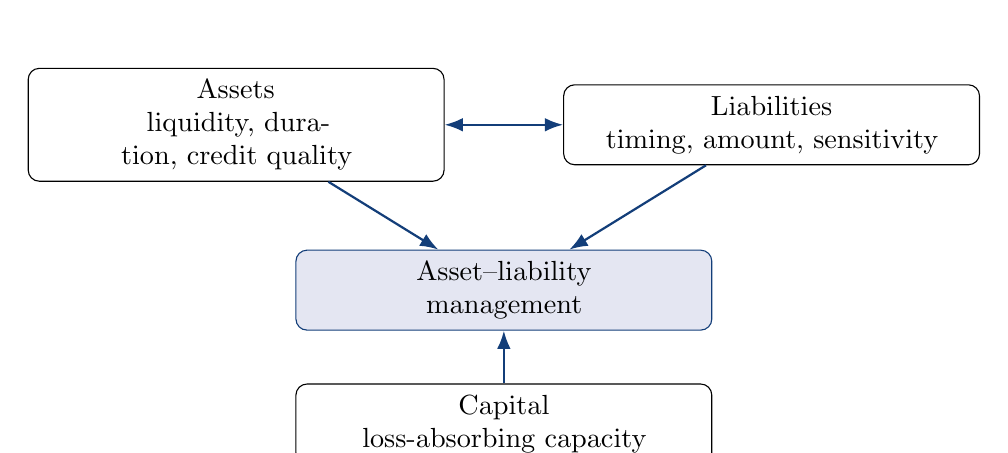
\begin{tikzpicture}[
> =Latex,
box/.style={
 draw,
 rounded corners,
 align=center,
 text width=5.0cm,
 minimum height=0.95cm,
 inner sep=4pt
 },
 main/.style={
 draw=FinanceBlue,
 fill=FinanceBlue!8,
 rounded corners,
 align=center,
 text width=5.0cm,
 minimum height=1.0cm,
 inner sep=4pt
 },
 flow/.style={-Latex, line width=0.8pt, FinanceBlue},
 link/.style={<->, line width=0.8pt, FinanceBlue}
 ]
\node[box] (assets) at (-3.4,1.6)
{Assets\\liquidity, duration, credit quality};

\node[box] (liab) at (3.4,1.6)
{Liabilities\\timing, amount, sensitivity};

\node[main] (alm) at (0,-0.5)
{Asset--liability \\ management};

\node[box] (capital) at (0,-2.2)
{Capital\\loss-absorbing capacity};

\draw[link] (assets) -- (liab);
\draw[flow] (assets) -- (alm);
\draw[flow] (liab) -- (alm);
\draw[flow] (capital) -- (alm);

\end{tikzpicture}

\caption{Asset--liability management and loss-absorbing capacity}
\label{fig}
\end{figure}


\section[Insurance Institutions and the Transfer of Risk]{Insurance Institutions and the Transfer of Risk}

Insurance institutions assume risks through insurance contracts but need not retain all of those risks on their own balance sheets. Depending on the nature and concentration of the exposure, insurers can retain risk, transfer part of it to reinsurers, or transfer selected risks to capital-market investors.

\subsection{Primary Insurers and Major Lines of Insurance}

Within the insurance system, primary insurers assume risks directly from households, firms, and other policyholders across major lines such as life, health, and property--casualty insurance.

Life insurance provides benefits linked to mortality or survival. Some contracts extend over long horizons and may include savings components, guarantees, or policyholder options, making liabilities sensitive to mortality, longevity, lapse behavior, and interest rates.

Health insurance covers medical expenses or specified health-related benefits. Claims can be frequent, while utilization may respond to coverage, making information and incentive problems important in many health insurance arrangements.

Property--casualty insurance covers property damage, liability, motor, business interruption, and other non-life risks. Claim settlement can range from relatively short periods to many years, while catastrophe events can generate large correlated losses across policies.

These differences translate into different liability profiles, affecting premium setting, reserve horizons, liquidity needs, asset--liability management, and the demand for reinsurance.



\begin{table}[H]

\centering

\caption{Selected insurance lines and liability characteristics}

\label{tab}

\begin{tabularx}{0.92\textwidth}{@{}p{0.20\textwidth} X X@{}}

\toprule

\textbf{Line} & \textbf{Typical insured exposure} & \textbf{Liability characteristics} \\

\midrule

Life insurance
& Mortality, survival, and long-term household protection
& Often long duration; may include guarantees and policyholder options \\

Health insurance
& Medical expenses and health-related benefits
& Claims may be frequent; utilization and information problems can be important \\

Property--casualty
& Property damage, liability, motor, and business interruption
& Claim duration varies by line; catastrophe and liability exposures can create large or delayed payments \\

\bottomrule

\end{tabularx}

\end{table}


\subsection{Reinsurance and the Redistribution of Insurance Risk}


The differences in liability profiles described above can create different needs for risk transfer. Reinsurance allows a primary insurer to transfer part of its underwriting exposure to a reinsurer in exchange for a reinsurance premium, thereby redistributing insured losses across institutions.


Reinsurance can limit exposure to individual large losses, reduce retained losses from catastrophe events, stabilize underwriting results, and increase the insurer's capacity to write additional business. The form of protection depends on how premiums and losses are divided between the primary insurer and the reinsurer.

Under proportional reinsurance, premiums and losses are shared according to an agreed proportion. If the reinsurer's share is $\alpha_R$, the ceded loss is

\begin{equation}
L_{\mathrm{ceded}}(L)=\alpha_R L.
\label{eq:ch15-proportional-reinsurance-payoff}
\end{equation}

Under excess-of-loss reinsurance, the reinsurer pays the portion of a covered loss above a retention $K$, subject to a maximum payment $M$:

\begin{equation}
L_{\mathrm{ceded}}(L)=\min\left\{\max(L-K,0),M\right\}.
\label{eq:ch15-excess-of-loss}
\end{equation}

The primary insurer therefore retains losses up to $K$ and any amount above $K+M$. The contract changes the insurer's retained-loss distribution, particularly in adverse states.

\begin{example}{Excess-of-Loss Reinsurance}{excess-loss-reinsurance}

An insurer purchases catastrophe reinsurance that attaches at RMB~100 million and provides a maximum payment of RMB~200 million.

If covered catastrophe losses are RMB~80 million, the reinsurer pays zero.

If losses are RMB~180 million, the reinsurer pays

\[
180-100=80
\]

million RMB.

If losses are RMB~400 million, the reinsurer pays the maximum RMB~200 million. The primary insurer retains the first RMB~100 million and the RMB~100 million above the reinsurance layer.

\end{example}

By accepting ceded risks from multiple primary insurers, a reinsurer can pool exposures across firms, regions, and lines of business. The resulting diversification depends on the dependence among those exposures, while highly correlated events can leave substantial risk concentrated at the reinsurance level.

Reinsurance also creates exposure to the reinsurer itself. The value of the protection therefore depends not only on the contractual terms, but also on the reinsurer's ability to meet its obligations when covered losses occur.


\subsection[Insurance-Linked Securities and Catastrophe Bonds]{Insurance-Linked Securities and Catastrophe \\Bonds}

Reinsurance transfers insurance risk to another insurance balance sheet, while insurance-linked securities can extend that transfer to capital-market investors. Catastrophe bonds are the most prominent example.

In a typical catastrophe bond structure, investor principal is placed in a collateral arrangement and investors receive compensation for bearing specified event risk. If no contractual trigger occurs during the risk period, the principal is returned at maturity. If the trigger is met, part or all of the principal is released according to the contract, reducing the sponsor's exposure to the covered event.

Let the bond principal be $F$. Abstracting from coupon payments, a terminal principal payoff is

\begin{equation}
X_T=
\begin{cases}
F, & \text{if no trigger event occurs},\\
(1-\theta)F, & \text{if the trigger produces a principal reduction of } \theta,
\end{cases}
\label{eq:ch15-cat-bond-payoff}
\end{equation}
where $0\leq\theta\leq1$ is determined by the contractual trigger and loss structure.

Triggers may be based on the sponsor's actual losses, industry losses, physical event parameters, modelled losses, or combinations of these measures. The choice of trigger affects the allocation of basis risk as well as the transparency and speed of settlement.

Catastrophe bonds broaden the sources of capital available to absorb concentrated insurance losses. They can complement reinsurance when catastrophe exposures are large or when additional risk-bearing capacity is valuable. Investors, in turn, receive compensation for assuming event risk that may have different drivers from conventional financial-market risks.

This transfer is not costless. Structuring expenses, modelling uncertainty, basis risk, legal arrangements, and required investor returns affect the economic value of the instrument. Insurance-linked securities therefore complement rather than mechanically replace traditional reinsurance.

\begin{tcolorbox}[
enhanced,
breakable,
colback=white,
colframe=FinanceBlue,
boxrule=0.7pt,
sharp corners,
borderline west={2.2pt}{0pt}{FinanceBlue},
title=\textbf{Financial Perspective: Extending Risk Transfer Beyond Insurance Balance Sheets},
coltitle=white,
colbacktitle=FinanceBlue,
fonttitle=\bfseries,
before skip=1.2em,
after skip=1.2em
]

Insurance risk can move through a sequence of balance sheets:

$$
\text{Policyholder}
\rightarrow
\text{Primary insurer}
\rightarrow
\text{Reinsurer}
\rightarrow
\text{Capital-market investor}.
$$

Each step redistributes the financial consequences of specified losses without eliminating the underlying uncertainty.

\end{tcolorbox}


%========================================================
% Summary
%========================================================

\TailModule{summary}{Summary}

Insurance reallocates uncertain losses through state-contingent contracts. Policyholders pay a known premium for protection against specified losses, while insurers pool exposures and maintain the financial capacity to meet claims.

Risk pooling can make losses more predictable across a large pool when individual losses are sufficiently weakly related. Correlation and common shocks limit this benefit and increase the need for capital and risk transfer.

Insurance contracts also balance risk sharing with incentives. Underwriting and risk classification address adverse selection, while deductibles, coinsurance, monitoring, and claims verification can mitigate moral hazard.

Pricing reflects expected losses, expenses, and the cost of bearing uncertainty. Reserves measure future obligations, asset--liability management coordinates assets with those liabilities, and capital provides loss-absorbing capacity.

Risk need not remain with the primary insurer. Reinsurance transfers exposures across insurance institutions, while insurance-linked securities can extend selected risks to capital-market investors.


%========================================================
% Key Terms
%========================================================

\TailModule{keyterms}{Key Terms}

Insurance; risk pooling; insurability; correlated losses; adverse selection; underwriting; moral hazard; deductibles and coinsurance; expected loss; risk loading; insurance liability; reserves; asset--liability management; solvency; reinsurance; catastrophe bonds; insurance-linked securities.

%========================================================
% Financial AI Lab
%========================================================

\TailModule{aiprompt}{Financial AI Lab}

\textbf{Lab: Audit an Insurance Pricing and Risk-Transfer Analysis}

Ask an AI system to analyze a simplified property insurer. Provide the number of policies, expected claim frequency, expected claim severity, operating expenses, a proposed premium or risk loading, a deductible, and a simplified aggregate excess-of-loss reinsurance layer.

Evaluate the analysis in four stages.

\begin{enumerate}

\item \textbf{Check expected loss and premium.}

Verify that claim frequency and conditional severity are combined consistently. Distinguish expected loss per policy from aggregate expected loss, and check how expenses and any risk loading enter the indicated premium.

\item \textbf{Inspect contract design.}

Examine how the deductible changes the insurer's payment and the policyholder's retained loss. Determine whether the information provided is sufficient to calculate its effect on expected claims; a mean loss alone may not identify the expected payout after a deductible. Separate any claims about moral hazard from the assumptions actually supplied.

\item \textbf{Trace the reinsurance layer.}

Apply several aggregate-loss outcomes below the attachment point, within the covered layer, and above its limit. Recalculate the reinsurer's payment and the primary insurer's retained loss in each case.

\item \textbf{Test a correlated-loss scenario.}

Replace independent claims with a catastrophe state that raises losses across many policies at the same time. Explain why a larger pool can reduce idiosyncratic variation without eliminating exposure to the common shock.

\end{enumerate}


%========================================================
% Discussion Questions
%========================================================

\TailModule{questions}{Discussion Questions}

\begin{enumerate}

\item Why can a risk-averse household be willing to pay an insurance premium above the expected loss?

\item How does the law of large numbers support risk pooling, and why does positive correlation limit this effect?

\item How do deductibles and coinsurance affect both risk sharing and policyholder incentives?

\item Why can a pooled premium create adverse-selection pressure when policyholders have private information about their own risk?

\item What is the economic distinction between insurance reserves and insurer capital?

\item How do reinsurance and catastrophe bonds redistribute insurance risk beyond the primary insurer?

\end{enumerate}


%========================================================
% Applied Problems
%========================================================

\TailModule{appprobs}{Applied Problems}


\begin{enumerate}

\item \textbf{Expected loss and insurance demand.}

A household faces a 3\% annual probability of a RMB~200,000 loss.

\begin{enumerate}

\item Calculate the expected annual loss. Compare the expected loss with an annual insurance premium of RMB~7,000.

\item Explain why a risk-averse household may still prefer the insurance contract.

\item Identify one factor other than risk aversion that could affect the household's decision.

\end{enumerate}

\item \textbf{Pooling independent claims.}

An insurer covers 25,000 similar risks. Each has a 2\% annual claim probability, and claim outcomes are independent.

\begin{enumerate}

\item Calculate the expected number of claims.

\item Calculate the standard deviation of the number of claims.

\item Calculate the standard deviation of claim frequency.

\item Explain how positive correlation among claim outcomes would affect the diversification benefit of pooling.

\end{enumerate}

\item \textbf{Deductibles and payment limits.}

A policy has a RMB~10,000 deductible and a maximum insurer payment of RMB~150,000.

\begin{enumerate}

\item Calculate the insurer's payment for losses of RMB~8,000, RMB~60,000, and RMB~250,000.

\item Calculate the insured's retained loss in each case.

\item Explain how the deductible affects policyholder incentives relative to full reimbursement from the first RMB of loss.

\end{enumerate}

\item \textbf{Premium decomposition.}

An insurer estimates an expected loss of RMB~1,800 per policy, expected expenses of RMB~450, and a risk loading of RMB~250.

\begin{enumerate}

\item Calculate the indicated premium under Equation~\ref{eq:ch15-premium-decomposition}.

\item Calculate the amount by which the indicated premium exceeds expected loss.

\item Express this amount as a percentage of the indicated premium.

\item Explain why the difference between premium and expected loss should not be interpreted as accounting profit.

\end{enumerate}

\item \textbf{Liability valuation and interest rates.}

An insurer expects to pay RMB~20 million in three years. Use a flat annual discount rate of 4\%.

\begin{enumerate}

\item Calculate the present value of the expected payment.

\item Recalculate the present value using a 3\% discount rate.

\item Explain the direction of the change.

\item Relate the result to the asset--liability management problem of a long-duration insurer.

\end{enumerate}

\item \textbf{Excess-of-loss reinsurance.}

A primary insurer retains the first RMB~50 million of aggregate catastrophe losses and purchases a reinsurance layer providing up to RMB~150 million above that retention.

\begin{enumerate}

\item Calculate the reinsurer's payment for aggregate losses of RMB~30 million, RMB~100 million, RMB~180 million, and RMB~260 million.

\item Calculate the primary insurer's retained loss in each case.

\item Identify the attachment point and exhaustion point of the reinsurance layer.

\item Explain how the contract changes the upper tail of the primary insurer's retained-loss distribution.

\end{enumerate}

\end{enumerate}


%========================================================
% Case Analysis
%========================================================

\TailModule{caseanalysis}{Case Analysis}

\textbf{Case: The 2021 Henan Floods and Insurance Risk Sharing}

Severe flooding struck Henan Province in July 2021, producing a large volume of insurance claims within a short period. By July 28, the province's insurance industry had received about 412,300 claim reports, with preliminary estimated insured losses of RMB~9.804 billion. About 43,400 claims had been settled, with claim payments of RMB~609 million at that point.\footnote{Henan provincial flood-relief press conference, July 29, 2021; official provincial information release published July 30, 2021, citing the Henan banking and insurance regulatory authority.}

The claims extended across several lines of insurance. Motor insurance accounted for about 226,400 reported claims and estimated losses of RMB~6.412 billion, while household-property and agricultural insurance also recorded substantial claims. The concentration of losses within the same region and event provides a useful setting for examining how insurance operates when many exposures are affected simultaneously.

Analyze the episode from four perspectives. First, explain how geographic correlation affects the diversification benefit of risk pooling. Second, examine how policy limits, exclusions, deductibles, and insured values can create differences between physical damage and insured losses. Third, explain why insurers may need liquidity while the final amount and timing of claims remain uncertain. Fourth, discuss how reinsurance can redistribute part of the loss retained by primary insurers.

The figures above were preliminary and should not be interpreted as final industry losses or claims payments.

\emph{Primary source context: Henan provincial flood-relief press conference, July 29, 2021; official provincial information release published July 30, 2021, citing the Henan banking and insurance regulatory authority.}


%========================================================
% Further Reading
%========================================================

\TailModule{furtherread}{Further Reading}

\begin{itemize}

\item Arrow, Kenneth J. (1963),
``Uncertainty and the Welfare Economics of Medical Care,''
\emph{American Economic Review}, 53(5), 941--973.

\item Pauly, Mark V. (1968),
``The Economics of Moral Hazard: Comment,''
\emph{American Economic Review}, 58(3), 531--537.

\item Rothschild, Michael, and Joseph E. Stiglitz (1976),
``Equilibrium in Competitive Insurance Markets: An Essay on the Economics of Imperfect Information,''
\emph{The Quarterly Journal of Economics}, 90(4), 629--649.

\item Froot, Kenneth A. (2001),
``The Market for Catastrophe Risk: A Clinical Examination,''
\emph{Journal of Financial Economics}, 60(2--3), 529--571.

\end{itemize}


\ChapterTail{summary,keyterms,aiprompt,questions,appprobs,caseanalysis,furtherread}

\chapter{Shadow Banking and Digital Financial Intermediation}
\label{chap:Shadow_Banking_and_Digital_Financial_Intermediation}

\begin{openingcase}{The Platform Says It Does Not Lend---So Who Made the Loan?}

A small merchant applies for a RMB~100,000 working-capital loan through a large digital commerce platform. The platform observes the merchant's sales and payment data, evaluates the application automatically, and displays an approved credit limit within minutes.

Yet the contract identifies a licensed financial institution as the lender. The platform provides customer access, data, scoring, and servicing, while the loan may later be transferred or refinanced through securities markets. The institution that originates the customer relationship need not ultimately hold the credit exposure.

If defaults rise, responsibility becomes less clear. Functions once combined inside a bank are distributed across platforms, financial institutions, and investors.

The central issue is where financial intermediation takes place, how funding moves through the chain, and where risk ultimately resides when bank-like credit intermediation extends beyond a single bank balance sheet.
\end{openingcase}

\begin{tcolorbox}[
  enhanced,
  colback=FinanceBlue!6,
  colframe=FinanceBlue,
  boxrule=0.6pt,
  sharp corners,
  left=8pt,
  right=8pt,
  top=7pt,
  bottom=7pt,
  before skip=1em,
  after skip=1.6em,
  title=\textbf{Core Questions},
  coltitle=white,
  colbacktitle=FinanceBlue,
  fonttitle=\bfseries,
  attach boxed title to top left={xshift=6pt,yshift=-2mm},
  boxed title style={boxrule=0pt,sharp corners,left=5pt,right=5pt,top=2pt,bottom=2pt}
]
\begin{enumerate}[leftmargin=*,label=\textcolor{FinanceBlue}{\textbf{\arabic*.}},itemsep=0.55em,topsep=0.2em]
\item Why can credit intermediation move outside traditional bank balance sheets, and which financial functions remain even when the institutional form changes?

\item How do funding chains, collateral, leverage, data, and digital platforms redistribute information production, liquidity transformation, and risk, and what new dependencies can arise in the process?
\end{enumerate}
\end{tcolorbox}

\section[The Evolution of Financial Intermediation Beyond Traditional Banking]{The Evolution of Financial Intermediation Beyond Traditional Banking}

Chapter 12 examined how commercial banks combine deposit funding, credit assessment, lending, monitoring, and liquidity creation within a regulated balance sheet. The present chapter extends that analysis beyond the traditional bank. Similar functions can be divided among finance companies, funds, broker-dealers, securitization vehicles, and digital platforms. The relevant change is not the disappearance of intermediation, but the redistribution of its funding, information, servicing, and risk-bearing functions across a wider institutional chain.

Financial intermediation does not require all functions to remain within a commercial bank. Credit origination, funding, servicing, and risk bearing can be separated and performed by different institutions. The institutional structure changes, but the underlying functions of screening, funding, monitoring, and risk allocation remain.

The key mechanism is the unbundling and recombination of these functions across balance sheets and markets. Regulation and capital constraints, specialization, capital-market development, and advances in data processing can all encourage this separation. Financial intermediation therefore evolves by reallocating familiar banking functions across institutions, contracts, and markets.


\subsection{Regulatory and Balance-Sheet Constraints}

A traditional bank combines funding, credit assessment, loan
origination, monitoring, liquidity provision, and risk bearing
within its balance sheet. Its capacity to perform these
functions depends on funding availability, capital adequacy,
liquidity conditions, and regulatory requirements. When the
cost of holding assets or performing particular functions
within this structure increases, institutions may have
incentives to separate certain stages of credit
intermediation from long-term balance-sheet holding.

One illustration is the equity-to-assets ratio. If a bank
seeks to maintain a target ratio, growth in total assets
must be accompanied by a corresponding increase in equity.
A loan retained on the balance sheet therefore uses part
of the bank's capacity to support additional credit exposure.
Selling or distributing the loan may reduce the resources
required to support that exposure, depending on the extent
of risk transfer and the obligations retained by the bank.

One response to these constraints is the originate-to-distribute
model. Under this arrangement, the originator may concentrate
on borrower acquisition, screening, structuring, and servicing,
while the funding and ownership of loans, together with part
of the associated credit exposure, are transferred to other
institutions. The originator may nevertheless retain some
exposures through guarantees, recourse arrangements, or
other contractual commitments.

Regulatory differences can strengthen this incentive. Banks,
securities firms, funds, finance companies, special-purpose
vehicles, and digital platforms operate under different
combinations of capital, liquidity, disclosure, conduct,
and activity requirements. When comparable financial
functions face different regulatory or balance-sheet costs
across institutional forms, those functions may be
reorganized across institutions and markets.

Such reorganization reallocates rather than eliminates
risk. Credit losses remain with the parties that retain
the relevant exposure, while liquidity, leverage,
operational, and model risks may arise at different stages
of the intermediation process.

\begin{tcolorbox}[
enhanced,
breakable,
colback=white,
colframe=FinanceBlue,
boxrule=0.7pt,
sharp corners,
borderline west={2.2pt}{0pt}{FinanceBlue},
title=\textbf{Financial Perspective: Moving an Asset Off a Bank Balance Sheet Does Not Remove Its Risk},
coltitle=white,
colbacktitle=FinanceBlue,
fonttitle=\bfseries,
before skip=1.2em,
after skip=1.2em
]

A loan may leave the originator's balance sheet through
sale, securitization, or another transfer arrangement.
Its underlying risks are redistributed among the institutions
that fund, insure, guarantee, service, or ultimately hold
the claim.

The key questions are who funds the asset, who bears credit
losses, who provides liquidity, and who controls underwriting
and servicing. These functions need not reside in the same
institution.

\end{tcolorbox}

\subsection[Specialization, Capital-Market Development, and Alternative Funding]{Specialization, Capital-Market Development,\ and Alternative Funding}

Regulatory and balance-sheet constraints help explain why some credit functions move outside traditional banks. A different mechanism arises from specialization and capital-market development. When origination, funding, servicing, and risk bearing can be performed separately, different institutions may concentrate on the functions in which they have comparative advantages.

A finance company may specialize in consumer or equipment credit, while a mortgage originator may focus on borrower acquisition and underwriting. Private credit funds can combine investor capital with direct-lending expertise, and securitization vehicles can connect pools of loans to capital-market investors. Such specialization can lower the cost of screening, origination, servicing, or risk bearing without requiring all functions to remain within one institution.

Capital-market development supports this separation by broadening the investor base and the instruments through which credit can be funded. In addition to deposits and bank wholesale liabilities, funding may be provided through bonds, asset-backed securities, fund shares, commercial paper, repurchase agreements, and other market-based claims. Borrowers can therefore be connected to investors through a sequence of contracts and intermediaries rather than through a single balance sheet.

The resulting funding chain may contain several layers. Investors may hold claims on a fund, the fund may finance a special-purpose vehicle, and the vehicle may hold loans originated by another institution. Funding moves toward the borrower, while contractual cash flows move in the opposite direction. The borrower's payments ultimately support the claims issued at earlier stages of the chain.

These arrangements can broaden funding sources and support specialization, but additional layers may also reduce transparency. Participants may have relatively good information about their immediate counterparties while having less visibility into leverage, collateral, liquidity commitments, or contingent exposures elsewhere in the chain.

\begin{figure}[htbp]
\centering
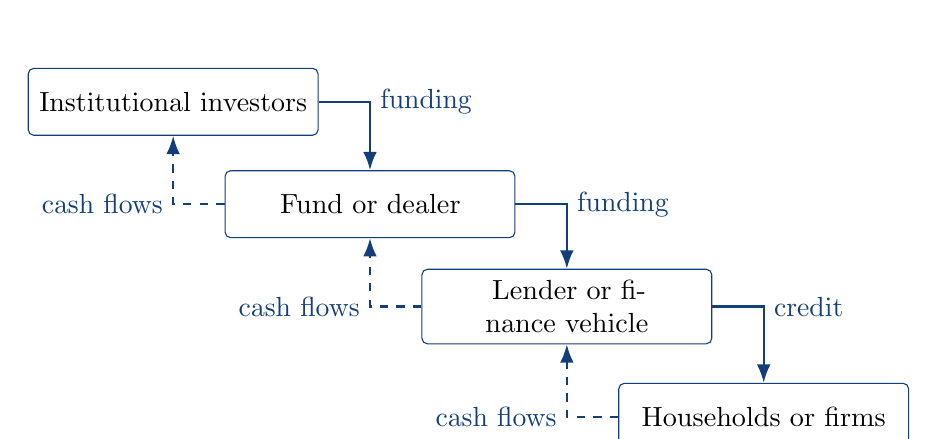
\begin{tikzpicture}[
  >=Latex,
 box/.style={
  draw=FinanceBlue,
  rounded corners=2pt,
  align=center,
  text width=3.4cm,
  minimum height=0.85cm,
  inner sep=4pt
},
  flow/.style={
    -Latex,
    line width=0.8pt,
    FinanceBlue
  },
  cashflow/.style={-Latex,dashed,line width=0.8pt,FinanceBlue}
]

% ------------------------------------------------
% Nodes: compact staircase layout
% ------------------------------------------------

\node[box] (investor) at (0,3.0)
  {Institutional investors};

\node[box] (fund) at (2.5,1.7)
  {Fund or dealer};

\node[box] (vehicle) at (5.0,0.4)
  {Lender or finance vehicle};

\node[box] (borrower) at (7.5,-1.0)
  {Households or firms};

% ------------------------------------------------
% Funding / credit: orthogonal arrows
% ------------------------------------------------

% Investors -> Fund
\draw[flow]
  (investor.east)
  -| node[pos=0.5,right]{funding}
  (fund.north);

% Fund -> Vehicle
\draw[flow]
  (fund.east)
  -| node[pos=0.5,right]{funding}
  (vehicle.north);

% Vehicle -> Borrower
\draw[flow]
  (vehicle.east)
  -| node[pos=0.5,right]{credit}
  (borrower.north);

% ------------------------------------------------
% Cash-flow return
% ------------------------------------------------

% Investors -> Fund
\draw[cashflow]
  (fund.west)
  -| node[pos=0.5,left]{cash flows}
  (investor.south);

  % Fund -> Vehicle
\draw[cashflow]
  (vehicle.west)
  -| node[pos=0.5,left]{cash flows}
  (fund.south);

% Vehicle -> Borrower
\draw[cashflow]
  (borrower.west)
  -| node[pos=0.5,left]{cash flows}
  (vehicle.south);

\end{tikzpicture}

\caption{A simplified market-based funding chain}
\label{fig:ch16-market-based-funding-chain}
\end{figure}

\subsection{Technology, Data, and Platform-Based Intermediation}

Digital technology changes how credit intermediation
produces information, reaches customers, and delivers
financial services. It can lower the costs of customer
acquisition, information processing, contract execution,
and loan servicing. Digital platforms can also draw on
data generated through payments, commerce, logistics,
and other economic activities, extending the information
available for credit assessment beyond conventional
financial records. Digital distribution can further
reduce dependence on physical branches and expand the
scale over which standardized financial services are
provided.

Data affects credit intermediation through two related
channels. First, additional information about borrower
activity can improve credit assessment and reduce some
information costs. Second, access to data and analytical
capabilities can alter organizational boundaries by
allowing one institution to control customer access
and credit assessment while another provides funding
or bears the associated risk. Information production,
credit decisions, and funding therefore need not remain
within the same institution.

The economic role of a platform depends on the functions
it performs and the exposures it retains. A platform may
connect borrowers with lenders, assess applicants,
recommend credit limits, originate or service loans,
collect payments, provide guarantees, or retain part
of the credit risk. Funding, contractual responsibility,
and loss-bearing capacity may reside with other
institutions. Platform-based intermediation is therefore
better understood by tracing the allocation of these
functions and exposures than by relying on institutional
labels.

Technology changes the organization of intermediation
rather than the underlying financial requirements.
Credit still requires funding, enforceable contracts,
servicing, loss absorption, and liquidity management.
Greater reliance on data, models, and digital
infrastructure, however, introduces operational
dependence and model risk. The efficiency gains from
digital intermediation therefore depend on the reliability
of information, the quality of decision models, and
the institutional arrangements governing the allocation
of risks and responsibilities.

\section{Shadow Banking and Market-Based Intermediation}

The shadow banking refers broadly to credit intermediation that performs bank-like functions outside the traditional deposit-taking banking system. These functions may include credit provision, maturity and liquidity transformation, and risk bearing, but they need not remain within a single bank balance sheet. Instead, they can be separated and recombined across institutions and markets.

Much of this intermediation is market-based, with funding raised through securities, fund shares, repos, and other contractual claims. Shadow banking emphasizes where bank-like functions are performed, while market-based intermediation emphasizes how funding is organized. The central analytical question is how credit, liquidity transformation, leverage, and risk are distributed across the intermediation chain.

\subsection{The Institutional Architecture of Shadow Banking}

Once bank-like functions are distributed across institutions and markets, credit intermediation becomes organized through a network of specialized intermediaries and contractual links. The relevant question is no longer which institution performs the entire process, but how funding, origination, servicing, liquidity provision, and risk bearing are allocated across the chain.

Finance companies may specialize in lending, money market funds in short-term investment, broker-dealers in securities financing and market making, and special-purpose vehicles in holding assets and issuing claims backed by their cash flows. Private credit funds combine investor capital with direct lending. These entities occupy different positions in the intermediation chain and differ in funding structure, leverage, redemption terms, liquidity exposure, and risk retention.

\begin{table}[H]

\centering

\caption{Selected forms of non-bank credit intermediation}

\label{tab:ch16-shadow-banking-institutions}

\begin{tabularx}{0.94\textwidth}{@{}p{0.23\textwidth} X X@{}}

\toprule

\textbf{Institution or structure} & \textbf{Primary function} & \textbf{Potential vulnerability} \\

\midrule

Finance company
& Specialized lending funded outside traditional deposits
& Credit losses and dependence on market or parent funding \\

Money market fund
& Pools investor funds and invests in short-term instruments
& Redemption pressure and liquidity stress under some structures \\

Broker-dealer
& Market making, securities financing, and inventory intermediation
& Leverage, collateral calls, and dependence on short-term funding \\

Special-purpose vehicle
& Holds assets and issues claims backed by their cash flows
& Asset performance, structural complexity, and refinancing risk in some structures \\

Private credit fund
& Direct lending funded by committed or pooled investor capital
& Credit concentration, valuation uncertainty, and borrower refinancing risk \\

\bottomrule

\end{tabularx}

\end{table}

Securitization illustrates how this architecture operates. An originator creates loans, a servicer collects payments, a special-purpose vehicle (SPV) holds the assets, an arranger structures the securities, and investors provide market funding. The underlying credit relationship remains, but funding, servicing, and risk bearing are distributed across a sequence of institutions and contracts.

\subsection{Funding Chains, Collateral, and Liquidity Transformation}

The institutional architecture described above becomes economically connected through funding chains. Investors provide funds to intermediaries, intermediaries finance assets or other institutions, and the resulting claims may extend through several balance sheets before reaching the ultimate borrower. In market-based intermediation, collateral often supports these links by securing short-term funding.

The amount of funding obtainable against collateral depends
on its market value and the applicable haircut, which is
the discount applied to collateral value when determining
borrowing capacity. A higher haircut reduces borrowing
capacity, potentially requiring additional collateral,
replacement funding, or asset sales.

This relation provides a channel through which stress can travel along the funding chain. If collateral values fall or haircuts rise, borrowers may need to post additional collateral, reduce borrowing, obtain replacement funding, or sell assets. When similar adjustments occur across several intermediaries, pressures in one part of the chain can affect others.

Liquidity transformation arises when claims held by investors or funding providers can be converted into cash relatively quickly while the underlying assets are less liquid or longer dated. An investment fund may offer frequent redemption while holding relatively illiquid credit assets, while a dealer may finance longer-dated securities with short-term repo. The degree of liquidity transformation depends on both the liquidity of the assets and the terms of the funding.

The same asset can therefore create different liquidity
pressures under different financing structures. A
long-maturity asset funded with stable equity creates
relatively little short-term refinancing pressure,
whereas the same asset financed through overnight
borrowing depends more heavily on continued market funding.

\begin{example}{A Haircut Shock and Funding Capacity}{haircut-funding-capacity}

A securities intermediary holds RMB~500 million of eligible collateral and initially finances the position at a 4\% haircut. Its borrowing capacity is

\[
B_0=(1-0.04)\times 500=480
\]

million RMB.

Suppose the collateral value remains unchanged but the haircut rises to 12\%. Borrowing capacity falls to

\[
B_1=(1-0.12)\times 500=440
\]

million RMB.

If the new haircut applies immediately, the intermediary
faces an RMB~40 million reduction in borrowing capacity.
It may respond by providing additional collateral,
repaying part of its borrowing, obtaining replacement
funding, or reducing the financed position.

\end{example}

\subsection{Leverage, Opacity, and Run Vulnerability}

The funding chains and liquidity transformation described above become more vulnerable when combined with leverage, limited transparency, and runnable funding. Leverage amplifies losses, opacity makes exposures more difficult to assess, and short-term funding can translate uncertainty into rapid balance-sheet adjustment.

Suppose an intermediary finances assets $A$ with liabilities $D$ and equity $E$, the leverage is $A/E$. If liabilities do not adjust immediately, a decline in asset value reduces equity by the same amount. A given\%age loss on assets therefore represents a larger\%age loss of equity when leverage is higher.

Opacity can amplify the resulting uncertainty. When creditors have limited information about asset quality, leverage, collateral reuse, off-balance-sheet commitments, or exposures elsewhere in the funding chain, losses may be difficult to locate and value. Uncertainty about where risk resides can weaken willingness to continue funding even before realized losses are fully known.

Runnable funding provides the channel through which this uncertainty can produce rapid adjustment. Investors may redeem claims, creditors may refuse renewal, or secured lenders may tighten financing terms. The intermediary may then need to replace funding, post additional collateral, or reduce assets within a short period. The extent of reliance on such funding can be expressed as

\begin{equation}
\phi=\frac{F_S}{A},
\label{eq:ch16-short-term-funding-ratio}
\end{equation}
where $F_S$ denotes short-term runnable or noncommitted funding. A higher $\phi$ indicates greater reliance on funding that may require frequent renewal, although actual vulnerability also depends on asset liquidity, collateral quality, committed backup funding, and the behavior of funding providers.

Run-like dynamics can therefore arise without traditional deposits. Redemptions from investment vehicles, nonrenewal of commercial paper, withdrawal of repo funding, and similar actions can force rapid balance-sheet adjustment when assets cannot be sold or refinanced on comparable terms.

\begin{tcolorbox}[
  enhanced,
  breakable,
  colback=white,
  colframe=FinanceBlue,
  boxrule=0.7pt,
  sharp corners,
  borderline west={2.2pt}{0pt}{FinanceBlue},
  title=\textbf{Financial Perspective: A Run Does Not Require a Deposit},
  coltitle=white,
  colbacktitle=FinanceBlue,
  fonttitle=\bfseries,
  before skip=1.2em,
  after skip=1.2em
]

A run is fundamentally a funding problem rather than a feature unique to deposits. It can occur whenever claims can be withdrawn or not renewed faster than the underlying assets can be converted into cash without substantial loss.

\end{tcolorbox}

\section[Platform Finance and Data-Driven Intermediation]{Platform Finance and Data-Driven \\Intermediation}

Platform finance combines digital customer networks, data, and automated decision systems with financial intermediation. By lowering information and distribution costs, it can separate customer access and credit assessment from funding and risk bearing.

\subsection{Platform Lending and Digital Credit Intermediation}

The separation of information production from funding and risk bearing is particularly visible in platform lending. Digital platforms can place customer acquisition, credit assessment, funding, servicing, and risk bearing in different institutions even when borrowers encounter a single interface.

The resulting arrangements vary. A marketplace platform may connect borrowers with investors or financial institutions, while a digital lender may use platform data to support its own credit decisions. In referral or co-lending arrangements, a licensed institution may provide funding while the platform contributes customer access, screening, or servicing. Similar digital interfaces can therefore represent different forms of credit intermediation.

A useful analytical framework separates five functions:
customer acquisition, underwriting, funding, servicing, risk bearing. These functions may be concentrated in one institution or distributed across several. The economic structure of platform lending depends on how they are allocated rather than on the interface presented to the borrower.

Suppose a platform facilitates RMB~1 billion of loans. Banks retain 80\% of the credit exposure, capital-market investors hold 15\% through securitized claims, and the platform retains 5\%. The platform may therefore play a central role in customer acquisition and underwriting while bearing only a small share of the ultimate credit risk.

This separation can support specialization, but it can also weaken the alignment between information production and loss bearing. When screening and risk bearing are divided across institutions, risk retention, guarantees, representations and warranties, monitoring rights, and servicing standards can help align incentives along the credit chain.

\begin{figure}[htbp]
\centering
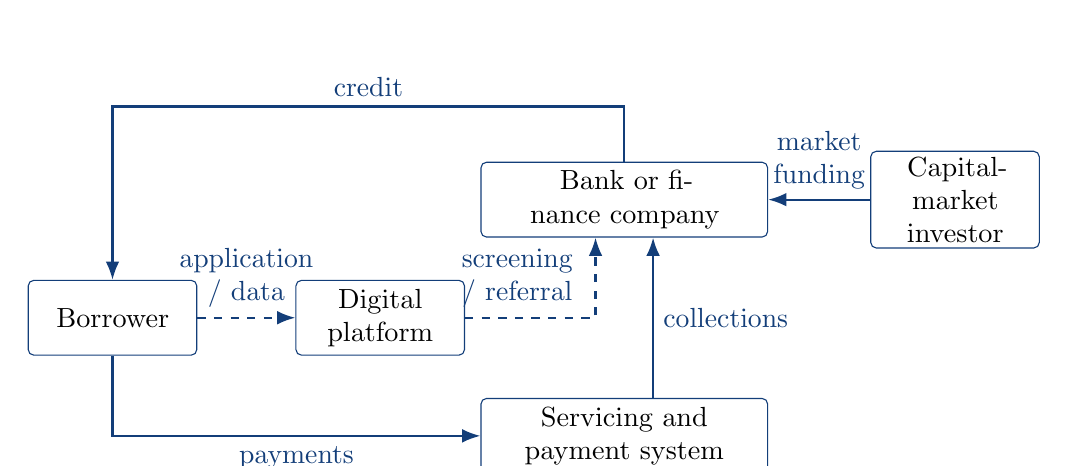
\begin{tikzpicture}[
  >=Latex,
  box/.style={
    draw=FinanceBlue,
    rounded corners=2pt,
    align=center,
    text width=2.0cm,
    minimum height=0.95cm,
    inner sep=2pt
  },
   finance/.style={
    draw=FinanceBlue,
    rounded corners=2pt,
    align=center,
    text width=3.5cm,
    minimum height=0.95cm,
    inner sep=2pt
  },
  flow/.style={
    -Latex,
    line width=0.8pt,
    FinanceBlue
  },
  info/.style={
    -Latex,
    dashed,
    line width=0.8pt,
    FinanceBlue
  }
]

% Nodes
\node[box] (borrower) at (0,0) {Borrower};

\node[box] (platform) at (3.4,0) {Digital\\platform};

\node[finance] (lender) at (6.5,1.5)
  {Bank or finance company};

\node[finance] (servicer) at (6.5,-1.5)
  {Servicing and payment system};

\node[box] (investor) at (10.7,1.5)
  {Capital-market\\investor};

% Information flows
\draw[info]
  (borrower.east)
  -- node[above,align=center]{application \\/ data}
  (platform.west);

\draw[info]
  (platform.east)
  -| node[pos=0.2,above,align=center]{screening \\ / referral}
  ($(lender.south west)!0.4!(lender.south east)$);

% Market funding
\draw[flow]
  (investor.west)
  -- node[above,align=center]{market \\funding}
  (lender.east);

% Credit from lender to borrower
\draw[flow]
  (lender.north)
  -- ++(0,0.70)
  -| node[pos=0.25,above]{credit}
  (borrower.north);

% Borrower payments to servicer
\draw[flow]
  (borrower.south)
  
  |- node[pos=0.75,below]{payments}
  (servicer.west);

% Collections passed to lender
\draw[flow]
  ($(servicer.north west)!0.6!(servicer.north east)$)
  -- node[right]{collections}
  ($(lender.south west)!0.6!(lender.south east)$);

\end{tikzpicture}

\caption{Separation of functions in digital credit intermediation}
\label{fig:ch16-platform-credit-chain}
\end{figure}

\subsection[Alternative Data, Credit Scoring, and Automated Underwriting]{Alternative Data, Credit Scoring, and Automated Underwriting}

When underwriting is performed digitally, the next question
is how information is converted into a credit decision.
Alongside financial statements, income, collateral, and
repayment history, lenders may use transaction records,
sales patterns, payment flows, logistics data, digital
interactions, and other legally permitted information.
Credit scoring and automated underwriting are used across
a range of lending markets, including consumer finance,
auto finance, mortgage lending, small-business credit,
and platform-based lending. The information used and
the relative importance of borrower characteristics,
repayment history, and collateral vary with the loan
product.

Credit-scoring models use available information about a
borrower, including financial characteristics, repayment
history, and other relevant indicators, to estimate the
borrower's probability of default. This estimate provides
a basis for credit classification, loan pricing, and
lending decisions.

The value of alternative data depends on whether they provide useful information beyond existing indicators or reduce screening costs. Additional data do not necessarily improve credit decisions: they may be noisy, selectively observed, unstable over time, or associated with legal and fairness concerns.

Credit scoring converts borrower information into a risk estimate; automated underwriting applies that estimate to lending decisions at scale. This can improve consistency and reduce processing time, but model errors can also be propagated across many applications.

Model performance therefore depends on both predictive accuracy and stability. Relationships observed in historical data may weaken when borrower behavior, platform activity, regulation, or economic conditions change.

Prediction and decision remain distinct. A lender must
translate estimated default risk into decisions about
loan approval, pricing, credit limits, maturity,
collateral requirements, and monitoring. The relevant
considerations vary across lending markets. In auto
finance, for example, lending decisions depend not only
on the borrower's repayment capacity but also on the
vehicle's value, expected depreciation, down payment,
and loan-to-value ratio. More generally, these decisions
depend on expected recoveries, funding costs, expected
returns, and the relative costs of different
classification errors.

\begin{example}{A More Accurate Score Does Not Automatically Produce a Better Lending Rule}{better-score-lending-rule}

Suppose a new model distinguishes high-risk from low-risk applicants more accurately than the previous model.

The lender must still determine how the predictions enter the approval rule. A stricter threshold may reduce expected credit losses but reject more applicants, while a looser threshold may expand lending while accepting more high-risk borrowers.

The economic value of the model therefore depends not only on predictive performance but also on how its predictions are translated into lending decisions.

\end{example}

\subsection[Embedded Finance and Platform Ecosystems]{Embedded Finance and Platform Ecosystems}

Data-driven financial services can be integrated directly into the commercial activities through which customer relationships and information are generated. Embedded finance places payments, credit, insurance, or other financial services within a non-financial transaction or platform relationship, such as working-capital credit in an e-commerce platform or installment financing at checkout.

Embedding can reduce distribution and transaction costs by offering financial services within an existing customer relationship and at the point of financial need. Information generated through the underlying transaction may also support servicing and monitoring when it is relevant and legally usable.

As financial and non-financial services become more closely integrated, the economics of individual products may depend on the wider platform ecosystem. A platform may accept a lower margin on one financial service when the relationship generates revenue elsewhere through commerce, payments, logistics, advertising, or other activities. Product economics therefore may extend beyond the standalone return on a loan, payment service, or insurance product.

Greater integration can also increase dependence on the platform. A merchant that relies on the same ecosystem for customers, payments, logistics, data, and finance may face higher switching costs and greater dependence on continued platform access. The financial effects therefore depend not only on product terms, but also on control over customer relationships, data, and distribution channels.

\begin{table}[H]

\centering

\caption{Economic mechanisms in embedded finance and platform ecosystems}

\label{tab:ch16-embedded-finance-ecosystems}

\begin{tabularx}{0.92\textwidth}{@{}p{0.27\textwidth} X@{}}

\toprule

\textbf{Platform feature} & \textbf{Financial implication} \\

\midrule

Existing customer relationship
& Can reduce acquisition and distribution costs by placing financial services within an established transaction channel \\

Integrated transactions
& Can provide financing, payment, or protection at the point of economic need \\

Ecosystem information
& Can support servicing and monitoring when the information is relevant and legally usable \\

Cross-selling
& Can make the economics of one financial product depend partly on revenues generated elsewhere in the ecosystem \\

Integrated ecosystem
& Can increase switching costs and dependence on platform access, data, and distribution channels \\

\bottomrule

\end{tabularx}

\end{table}

\section[Changing Boundaries and Market Power in Financial Intermediation]{Changing Boundaries and Market Power in Financial Intermediation}

Digital and market-based intermediation can separate information, distribution, servicing, funding, and risk bearing across different institutions, changing the boundary between markets and intermediaries. As these functions are reorganized, control over customer access, data, networks, and distribution channels can become a source of market power, leading to reintermediation rather than the disappearance of intermediaries.

\subsection[Disintermediation, Reintermediation, and Financial Ecosystems]{Disintermediation, Reintermediation, and Financial Ecosystems}

The integration of finance into digital ecosystems changes not only how financial services are delivered, but also which intermediaries connect customers with funding. Disintermediation occurs when financing bypasses an existing intermediary. A firm that replaces a bank loan with a bond issue, for example, reduces its reliance on bank balance-sheet intermediation.

The functions of intermediation, however, do not disappear. Bond finance still requires issuance, distribution, custody, trading, and investment management, while securitization separates origination, funding, servicing, and risk bearing across several entities. When these functions are reassigned to a new set of intermediaries, the process is better described as reintermediation.

Digital platforms extend this process by organizing customer access, data, and distribution within a financial ecosystem. A platform may reduce reliance on branches or traditional distribution channels while becoming an important interface between customers and financial institutions. Its role may depend less on deposit funding or direct asset holding than on control over customer access, information, and transaction flows.

As institutional boundaries become less informative, analysis can focus on how financial functions and exposures are allocated. A functional map asks four questions:

\begin{enumerate}

\item Who controls the customer relationship?

\item Who produces, controls, or has access to the information used in financial decisions?

\item Who provides funding and liquidity?

\item Who ultimately bears financial losses?

\end{enumerate}

These questions provide a common framework for comparing banks, platforms, funds, securitization structures, and hybrid forms of intermediation.

\subsection[Data Concentration, Market Power, and Algorithmic Dependence]{Data Concentration, Market Power, and Algorithmic Dependence}

As financial ecosystems become organized around digital platforms, control over customer relationships, transaction flows, and data can become increasingly concentrated. A larger user base generates more activity and information, which may improve services and reduce average information-processing and distribution costs. Better services can in turn attract additional users and generate further data.

This feedback can strengthen market position when customer networks, proprietary data, or distribution channels are difficult to replicate. Entrants may have comparable technology but less transaction history, fewer established users, or weaker access to customer relationships. Data scale can therefore affect both operating efficiency and market contestability.

Market power may arise through network effects, switching costs, control over data and digital interfaces, integration across services, and established customer relationships. These advantages can influence fees, product placement, access to customers, and bargaining power between platforms and financial institutions.

Digital concentration can also arise through common dependence rather than common ownership. Financial institutions may remain legally separate while relying on the same cloud services, data providers, scoring systems, or similar model architectures. If these common inputs fail or generate similar errors, decisions across institutions may become more correlated.

Shared technology can lower costs and improve consistency, but dependence on a limited set of providers, data sources, or models may also create operational concentration and reduce substitutability under stress. The financial significance of digital concentration therefore depends on how efficiency gains interact with contestability, common exposure, and financial resilience.

\begin{tcolorbox}[
  enhanced,
  breakable,
  colback=white,
  colframe=FinanceBlue,
  boxrule=0.7pt,
  sharp corners,
  borderline west={2.2pt}{0pt}{FinanceBlue},
  title=\textbf{Financial Perspective: Digital Scale Can Reduce Cost and Concentrate Dependence},
  coltitle=white,
  colbacktitle=FinanceBlue,
  fonttitle=\bfseries,
  before skip=1.2em,
  after skip=1.2em
]

Digital scale can create efficiency and concentration through the same underlying mechanism. The analytical question is whether gains from scale are accompanied by dependence on data, interfaces, models, or infrastructure that is difficult to replace.

\end{tcolorbox}

%========================================================
% Summary
%========================================================

\TailModule{summary}{Summary}

Financial intermediation can move beyond traditional bank balance sheets without eliminating its underlying functions. Credit still requires information production, contracting, funding, servicing, liquidity management, and risk bearing. Shadow banking is therefore best understood as an architecture in which these functions are distributed across non-bank institutions, markets, and contractual funding chains.

Collateral, leverage, and short-term funding influence how this architecture responds to stress. Haircuts link borrowing capacity to collateral values, while runnable funding and leverage can amplify balance-sheet adjustment. Run-like pressure may arise through redemptions or funding withdrawal even when deposits are absent.

Digital platforms extend this reorganization by combining customer networks, data, automated underwriting, and embedded financial services. They can reduce information and distribution costs while separating customer access and credit assessment from funding and risk bearing. As intermediation is reorganized, disintermediation may be followed by reintermediation, while data concentration, network effects, switching costs, and common digital infrastructure can create new forms of market power and dependence. The central analytical task remains to identify who performs each financial function and where the associated risks ultimately reside.

%========================================================
% Mind Map
%========================================================

\TailModule{mindmap}{Mind Map}

\begin{figure}[H]
\centering
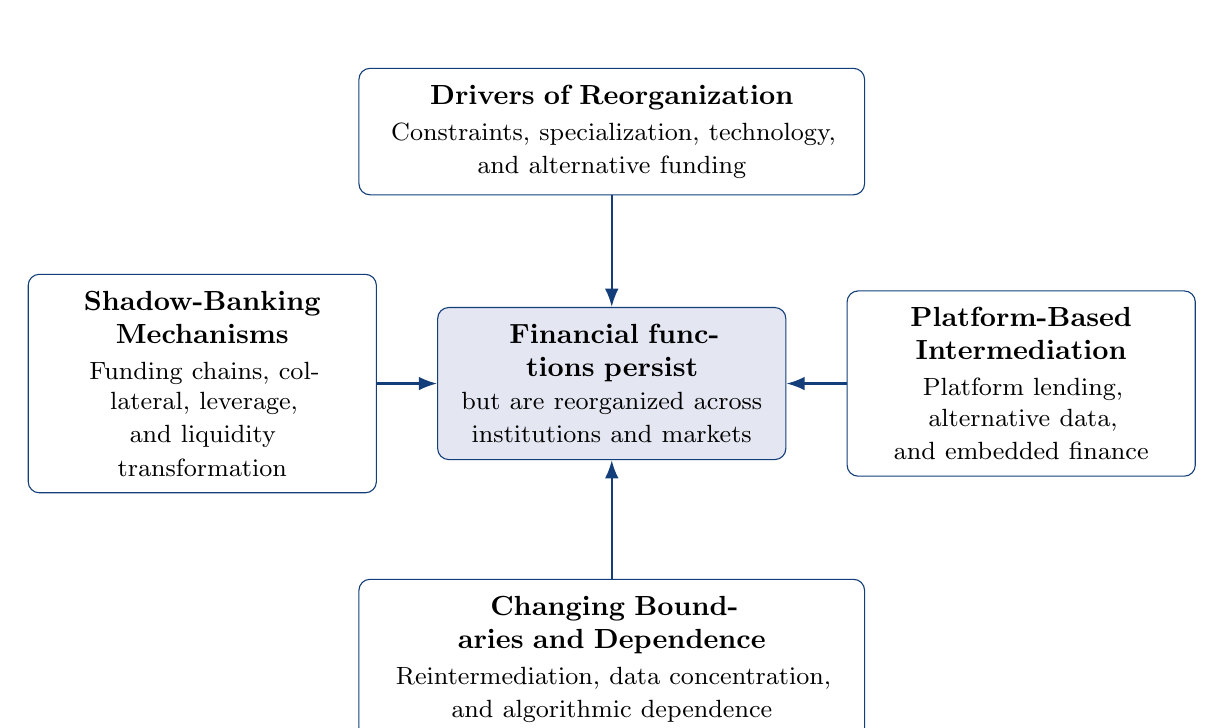
\begin{tikzpicture}[
  >=Latex,
  center/.style={
    draw=FinanceBlue,
    fill=FinanceBlue!8,
    rounded corners,
    align=center,
    text width=4.0cm,
    minimum height=1.1cm,
    inner sep=6pt
  },
  box/.style={
    draw=FinanceBlue,
    rounded corners,
    align=center,
    text width=4.0cm,
    minimum height=1.15cm,
    inner sep=6pt
  },
  middle/.style={
    draw=FinanceBlue,
    rounded corners,
    align=center,
    text width=6.0cm,
    minimum height=1.15cm,
    inner sep=6pt
  },
  flow/.style={
    -Latex,
    line width=0.8pt,
    FinanceBlue
  }
]

\node[center] (core) at (0,0)
{\textbf{Financial functions persist}\\
{\small but are reorganized across institutions and markets}};

\node[middle] (drivers) at (0,3.2)
{\textbf{Drivers of Reorganization}\\[2pt]
{\small Constraints, specialization, technology,\\
and alternative funding}};

\node[box] (shadow) at (-5.2,0.0)
{\textbf{Shadow-Banking Mechanisms}\\[2pt]
{\small Funding chains, collateral, leverage,\\
and liquidity transformation}};

\node[box] (platform) at (5.2,0.0)
{\textbf{Platform-Based Intermediation}\\[2pt]
{\small Platform lending, alternative data,\\
and embedded finance}};

\node[middle] (boundary) at (0,-3.5)
{\textbf{Changing Boundaries and Dependence}\\[2pt]
{\small Reintermediation, data concentration,\\
and algorithmic dependence}};

\draw[flow] (drivers) -- (core);
\draw[flow] (shadow) -- (core);
\draw[flow] (platform) -- (core);
\draw[flow] (boundary) -- (core);

\end{tikzpicture}

\caption{Financial functions persist even when institutional boundaries change.}
\label{fig:ch16-summary-map}
\end{figure}

%========================================================
% Key Terms
%========================================================

\TailModule{keyterms}{Key Terms}

Shadow banking; market-based intermediation; originate-to-distribute;
securitization; funding chain; collateral; haircut; liquidity transformation;
leverage; run vulnerability; platform lending; alternative data;
automated underwriting; embedded finance; reintermediation;
network effects; data concentration; algorithmic dependence.

%========================================================
% Financial AI Lab
%========================================================

\TailModule{aiprompt}{Financial AI Lab}

\textbf{Lab: Reconstruct a Digital Credit Chain}

Choose a real digital lending or embedded-finance arrangement and ask an AI system to explain how the product works. Treat the initial answer as a hypothesis rather than as verified fact.

Use primary sources from the platform, lender, regulator, prospectus, securitization documents, or other relevant disclosures to reconstruct the financing chain.

\begin{enumerate}

\item Identify who acquires the customer, performs credit assessment, makes the formal lending decision, provides funding, services the loan, and ultimately bears credit losses.

\item Compare this structure with the AI answer. Check whether it confuses the consumer-facing platform with the legal lender, funding provider, or ultimate risk holder.

\item Identify guarantees, risk-sharing arrangements, loan transfers, securitization, or other mechanisms that affect where credit exposure resides.

\item Examine the documented information used in credit assessment. Distinguish disclosed data inputs from assumptions about model design, weighting, or predictive performance.

\item Identify one important risk that remains even if credit prediction improves, such as funding, liquidity, operational, legal, or concentration risk.

\end{enumerate}

%========================================================
% Discussion Questions
%========================================================

\TailModule{questions}{Discussion Questions}

\begin{enumerate}

\item Why can transferring a loan away from the originator's balance sheet expand lending capacity without eliminating credit risk?

\item How can an increase in repo haircuts reduce an intermediary's funding capacity even when the market value of collateral is unchanged?

\item How can non-bank intermediaries perform bank-like functions without accepting traditional deposits?

\item In platform lending, why can customer acquisition, underwriting, funding, and risk bearing be performed by different institutions?

\item How can alternative data improve credit assessment while also creating concerns about model stability, data use, and concentration?

\item Why can digital finance produce reintermediation, and how can reliance on common algorithms, data sources, or technology providers create shared exposures across otherwise separate institutions?

\end{enumerate}

%========================================================
% Data Application
%========================================================

\TailModule{dataapp}{Data Application}

\textbf{Mapping Non-Bank and Digital Credit Intermediation in China}

Use authoritative Chinese sources such as the People's Bank of China, the National Financial Regulatory Administration, the China Securities Regulatory Commission, exchange or interbank-market disclosures, asset-backed securities documents, and published disclosures of financial institutions or digital platforms.

Select one credit channel outside a conventional bank loan, such as consumer-finance companies, asset-backed securities, trust financing, private credit or private fund structures where applicable, or a platform-based lending arrangement.

Construct a financing map showing the borrower, originator, formal lender where applicable, funding provider, servicer, guarantor or other credit-enhancement provider, and ultimate investor or risk holder where identifiable. If the structure changes over time, document the sequence rather than combining different periods into one static map.

Collect at least three quantitative indicators that are economically linked to the financing chain. These may include outstanding financing, issuance volume, funding composition, asset-pool characteristics, delinquency measures, investor composition, or platform loan facilitation where primary disclosures are available.

Interpret the evidence through financial functions rather than institutional labels. Identify who produces information, who provides funding, who bears credit losses, and which participants depend on market refinancing. State any important limitation arising from consolidated reporting, incomplete disclosure, or unavailable information on risk retention.

%========================================================
% Case Analysis
%========================================================

\TailModule{caseanalysis}{Case Analysis}

\textbf{Case: China's P2P Lending Boom---Was the Platform Only an Information Intermediary?}

Peer-to-peer Internet lending expanded rapidly in China during the 2010s. The regulatory framework defined P2P platforms primarily as information intermediaries connecting borrowers with lenders rather than as deposit-taking institutions. In practice, business models varied, and the boundary between information matching, credit enhancement, funding transformation, and risk bearing was not always easy for investors to identify.

As risks accumulated, Chinese authorities conducted a multi-year rectification of Internet finance and P2P lending. A People's Bank of China report stated that the number of operating P2P Internet lending institutions fell from a peak of around 5,000 to 29 by the end of June 2020.

Analyze the episode as a problem of financial architecture rather than as a chronology of regulation.

First, reconstruct the basic P2P claim structure. Who supplied funds, who borrowed, and what legal and economic roles did the platform perform? Second, examine whether guarantees, affiliated entities, pooled funding, maturity transformation, or other arrangements moved the platform beyond pure information matching. Third, explain why complex contractual chains could make the location of credit and liquidity risk difficult for investors to identify. Fourth, compare the P2P structure with the commercial-bank model in Chapter~12: which intermediation functions were similar, and which funding, capital, liquidity, or loss-absorption arrangements were different?

The case illustrates a central theme of this chapter: institutional labels do not by themselves determine the economic structure of credit intermediation. The analysis begins with functions, contracts, funding, and risk allocation.

\emph{Primary source context: People's Bank of China, ``Firmly Fight the Critical Battle of Preventing and Defusing Financial Risks''; \emph{Interim Measures for the Administration of the Business Activities of Online Lending Information Intermediaries}, 2016.}

%========================================================
% Further Reading
%========================================================

\TailModule{furtherread}{Further Reading}

\begin{itemize}

\item Adrian, Tobias, and Hyun Song Shin (2010),
``Liquidity and Leverage,''
\emph{Journal of Financial Intermediation}, 19(3), 418--437.

\item Gorton, Gary, and Andrew Metrick (2012),
``Securitized Banking and the Run on Repo,''
\emph{Journal of Financial Economics}, 104(3), 425--451.

\item Pozsar, Zoltan, Tobias Adrian, Adam Ashcraft, and Hayley Boesky (2013),
``Shadow Banking,''
\emph{Federal Reserve Bank of New York Economic Policy Review}, 19(2), 1--16.

\item Buchak, Greg, Gregor Matvos, Tomasz Piskorski, and Amit Seru (2018),
``Fintech, Regulatory Arbitrage, and the Rise of Shadow Banks,''
\emph{Journal of Financial Economics}, 130(3), 453--483.

\item Berg, Tobias, Valentin Burg, Ana Gombovi\'c, and Manju Puri (2020),
``On the Rise of FinTechs: Credit Scoring Using Digital Footprints,''
\emph{The Review of Financial Studies}, 33(7), 2845--2897.
\end{itemize}

\ChapterTail{summary,mindmap,keyterms,aiprompt,questions,dataapp,caseanalysis,furtherread}


\part{Financial Instruments and Risk Management}
\chapter{Linear Derivatives: Forwards, Futures, and Swaps}
\label{chap:Linear_Derivatives_Forwards_Futures_and_Swaps}

\begin{openingcase}{The Hedge Lost Money---Did It Fail?}

A copper-products manufacturer expects to purchase 1,000 tonnes of copper in three months. To protect its budget against a price increase, it takes a long position in copper futures at RMB~80,000 per tonne.

One month later, copper prices fall sharply. The physical purchase will cost less, but the futures position loses money and requires variation margin. Once the futures loss is included, the firm's hedged purchase cost is not necessarily lower. 

\end{openingcase}


\begin{tcolorbox}[
  enhanced,
  colback=FinanceBlue!6,
  colframe=FinanceBlue,
  boxrule=0.6pt,
  sharp corners,
  left=8pt,
  right=8pt,
  top=7pt,
  bottom=7pt,
  before skip=1em,
  after skip=1.6em,
  title=\textbf{Core Questions},
  coltitle=white,
  colbacktitle=FinanceBlue,
  fonttitle=\bfseries,
  attach boxed title to top left={xshift=6pt,yshift=-2mm},
  boxed title style={
    boxrule=0pt,
    sharp corners,
    left=5pt,
    right=5pt,
    top=2pt,
    bottom=2pt
  }
]
\begin{enumerate}[
  leftmargin=*,
  label=\textcolor{FinanceBlue}{\textbf{\arabic*.}},
  itemsep=0.55em,
  topsep=0.2em
]



\item How do forward and futures contracts manage exposure to uncertain future prices, and how does no-arbitrage link contract prices to spot prices and financing costs?

\item How do standardization, margining, and central clearing alter liquidity, counterparty exposure, and the institutional structure of futures markets?

\item How do swaps extend a single future exchange into a sequence of cash-flow exchanges in interest-rate and currency markets?



\end{enumerate}
\end{tcolorbox}


\section{Forward Contracts and Bilateral Commitments}

A forward contract is a bilateral agreement that fixes today the terms of an exchange that will occur at a future date. The contract can be written on currencies, commodities, securities, interest rates, or other measurable financial quantities. Its defining feature is a linear payoff: gains to one side move one-for-one with losses to the other side as the underlying price changes.


\subsection{Contract Terms, Delivery, and Settlement}

A forward contract specifies the underlying asset or reference price, notional quantity, maturity date, settlement terms, and delivery price $K$. At inception, $K$ is typically set so that the contract has approximately zero market value to both parties. For a long forward on one unit of an asset, the payoff at maturity $T$ is

\begin{equation}
X_T=S_T-K,
\label{eq:ch17-forward-payoff}
\end{equation}
where $S_T$ is the spot price at maturity. The short position has the opposite payoff. The maturity payoff has a linear profile in \(S_T\), with a constant slope of \(+1\) for the long position and \(-1\) for the short position.

Settlement may take the form of physical delivery or cash settlement. Under physical delivery, the long pays the contracted amount and receives the underlying asset. Under cash settlement, the parties exchange the difference between the contracted price and the specified settlement price. The operational cash flows differ, but the resulting price exposure can be broadly similar. For a contract covering $Q$ units, the long payoff is

\begin{equation}
X_T=Q(S_T-K).
\label{eq:ch17-forward-payoff-quantity}
\end{equation}

The quantity $Q$ determines the scale of the exposure. In a cash-settled contract, it serves as the basis for calculating the settlement payment rather than representing an amount that is itself exchanged.

\begin{example}{A Commodity Forward}{commodity-forward-payoff}

A manufacturer expects to purchase 500 tonnes of metal in six months and enters a cash-settled forward at RMB~18,000 per tonne.

If the spot price at maturity is RMB~19,200, purchasing the metal in the spot market costs

\[
500 \times 19{,}200
=
9{,}600{,}000
\]

RMB. The long forward produces a payoff of

\[
500(19{,}200-18{,}000)
=
600{,}000.
\]

The forward gain offsets part of the physical purchase cost, leaving an effective cost of

\[
9{,}600{,}000-600{,}000
=
9{,}000{,}000,
\]

or RMB~18,000 per tonne.

If the spot price instead falls to RMB~17,400, the physical purchase costs RMB~8,700,000, while the forward produces a loss of RMB~300,000. The combined cost is again

\[
8{,}700{,}000+300{,}000
=
9{,}000{,}000,
\]

or RMB~18,000 per tonne.

The forward therefore offsets changes in the spot purchase price when the contract closely matches the planned transaction, abstracting from basis differences, credit exposure, transaction costs, and funding effects.

\end{example}

A forward with approximately zero value at inception can later acquire positive or negative market value as the underlying price and other market conditions change. Before maturity, a forward position may be unwound through an offsetting contract or an agreed early termination. An offsetting contract reduces the economic exposure but does not necessarily extinguish the original contractual obligation.

\subsection{Forward Pricing and the Cost-of-Carry Relation}

Forward pricing follows from no-arbitrage. If two strategies generate the same payoff at a future date, their current costs should be consistent after financing and other relevant carrying components are taken into account.

Consider an asset that pays no income and can be held without storage cost. Let $S_0$ be the spot price, $r$ the continuously compounded financing rate, and $T$ the time to maturity. An investor can buy the asset today and finance the purchase until $T$. The amount required to repay the financed purchase at maturity is

\[
S_0 e^{rT}.
\]

No-arbitrage therefore implies

\begin{equation}
F_{0,T}=S_0 e^{rT}.
\label{eq:ch17-basic-forward-price}
\end{equation}

For a newly initiated forward at market terms, the delivery price is set equal to the prevailing forward price, so that $K=F_{0,T}$ at inception.

The no-arbitrage mechanism can be seen directly. If the market forward price exceeds $S_0e^{rT}$, a trader can borrow $S_0$, buy the asset in the spot market, and take a short forward position. At maturity, the asset is delivered for $F_{0,T}$ and the borrowing is repaid for $S_0e^{rT}$. The difference,
\[
F_{0,T}-S_0e^{rT},
\]
is an arbitrage profit under the stated assumptions.

If the forward price is below $S_0e^{rT}$, the reverse strategy can be used when short selling is feasible. The trader shorts the asset, invests the proceeds $S_0$, and takes a long forward position. At maturity, the investment grows to $S_0e^{rT}$; the trader pays $F_{0,T}$ under the forward contract, receives the asset, and returns it to the lender. The resulting arbitrage profit is

\[
S_0e^{rT}-F_{0,T}.
\]

These strategies link the forward price to the spot price and the cost of carrying the asset to maturity. In practice, transaction costs, financing conditions, and short-selling constraints can weaken the arbitrage mechanism.

The cost-of-carry relation extends the same logic to assets that provide income or involve additional holding costs. If the asset provides a continuously compounded income yield $q$, the forward price becomes

\begin{equation}
F_{0,T}=S_0 e^{(r-q)T}.
\label{eq:ch17-forward-price-income-yield}
\end{equation}

Here the net cost of carry reflects financing cost less the income earned from holding the asset.

For a foreign currency, the foreign interest rate plays a role similar to an income yield on the foreign-currency asset. Under no-arbitrage conditions, this relationship implies covered interest parity:

\begin{equation}
F_{0,T}=S_0 e^{(r_d-r_f)T},
\label{eq:ch17-fx-forward-relation}
\end{equation}
where $r_d$ and $r_f$ are the domestic and foreign interest rates.

For commodities, storage and other carrying costs can increase the net cost of carry, while the benefit of holding physical inventory---often represented by a convenience yield---can work in the opposite direction. Under a proportional continuous-rate convention,

\begin{equation}
F_{0,T}=S_0 e^{(r+u-y)T},
\label{eq:ch17-commodity-cost-of-carry}
\end{equation}
where $u$ denotes the storage-cost rate and $y$ the convenience yield.

\begin{tcolorbox}[
  enhanced,
  breakable,
  colback=white,
  colframe=FinanceBlue,
  boxrule=0.7pt,
  sharp corners,
  borderline west={2.2pt}{0pt}{FinanceBlue},
  title=\textbf{Financial Perspective: Forward Price Is Not a Forecast},
  coltitle=white,
  colbacktitle=FinanceBlue,
  fonttitle=\bfseries,
  before skip=1.2em,
  after skip=1.2em
]

The forward price is linked to the spot price through financing, income, storage, and other carry components. It therefore need not equal the market's expected future spot price.

A forward can have zero value at inception even when the realized spot price at maturity differs substantially from its delivery price.

\end{tcolorbox}

\begin{example}{Cost of Carry for a Non-Income Asset}{forward-cost-of-carry-example}

An asset has a spot price of RMB~100 and can be financed for one year at a continuously compounded rate of 4\%. It pays no income and has no storage cost.

The no-arbitrage forward price is

\[
F_{0,1}=100e^{0.04\times 1}\approx104.08.
\]

If the market forward price were RMB~110, the cash-and-carry strategy described above would produce a difference of approximately RMB~5.92 per unit before transaction costs and other market frictions.

\end{example}

The forward price should be distinguished from the value of an existing forward contract. Once a contract has been initiated, its delivery price $K$ remains fixed, while the market forward price for the same maturity can change. At time $t<T$, the value to the long can be written as

\begin{equation}
V_t=D(t,T)\left(F_{t,T}-K\right),
\label{eq:ch17-forward-value-general}
\end{equation}
where $D(t,T)$ is the discount factor from $T$ to $t$. The contract has positive value to the long when $F_{t,T}>K$ and negative value when $F_{t,T}<K$.

\subsection{Hedging Future Cash Flows}

A forward hedge combines a derivative position with an existing or expected commercial or financial exposure. Its purpose is to reduce the sensitivity of the combined cash flow to an uncertain future price.

A firm that expects to buy an asset can take a long hedge, while a firm that expects to sell an asset can take a short hedge. The forward position is chosen so that changes in its payoff offset changes in the underlying cash flow.

Suppose a manufacturer will purchase $Q$ units of a commodity at date $T$. Without hedging, the purchase cost is

\begin{equation*}
C_T=QS_T.
\label{eq:ch17-unhedged-purchase-cost}
\end{equation*}

If the manufacturer takes a long forward on the same quantity, underlying asset, and maturity at delivery price $K$, the forward payoff is $Q(S_T-K)$. Measuring the forward payoff against the physical purchase cost gives

\begin{equation*}
QS_T-Q(S_T-K)=QK.
\label{eq:ch17-perfect-long-forward-hedge}
\end{equation*}

Under these matching assumptions, the uncertain purchase price is replaced by the contracted price $K$.

The same mechanism applies to a future sale. A producer that expects to sell $Q$ units at date $T$ can take a short forward with payoff $Q(K-S_T)$. Combining this payoff with spot revenue gives

\begin{equation*}
QS_T+Q(K-S_T)=QK.
\label{eq:ch17-perfect-short-forward-hedge}
\end{equation*}

Thus, under the same matching assumptions, the forward stabilizes the effective sale price at $K$.

\begin{example}{A Short Forward Hedge}{short-forward-hedge}

A copper producer expects to sell 1,000 tonnes of copper in three months and takes a short forward at RMB~80,000 per tonne.

If the spot price at maturity falls to RMB~74,000, the physical sale generates RMB~74 million, while the short forward produces a gain of RMB~6 million. The combined revenue is therefore RMB~80 million, or RMB~80,000 per tonne.

The forward gain offsets the decline in the cash-market selling price, illustrating how a short hedge can stabilize future revenue when the contract closely matches the underlying exposure.

\end{example}

Forward contracts can be tailored to the quantity, maturity, reference asset, and settlement terms of a specific exposure. This flexibility can improve hedge matching. At the same time, a bilateral forward depends on the performance of the counterparty, making credit and settlement arrangements an important part of the contract.

\subsection{Counterparty Risk and Bilateral Risk Management}

Because an existing forward can acquire positive or negative market value, a bilateral contract can create counterparty exposure. If a counterparty defaults while the contract has positive value to the other party, part of the value needed to replace the contract in the market may be lost.

For a party holding a forward contract with current value
$V_t$, the current replacement exposure before collateral
and netting is

\begin{equation}
E_t=\max(V_t,0).
\label{eq:ch17-forward-current-exposure}
\end{equation}

This exposure is distinct from the notional amount. A forward with a notional amount of RMB~100 million may have a replacement exposure of only a fraction of that amount, depending on market movements and contract terms.

Bilateral contracts can use collateral to limit unsecured exposure. Without collateral, the market value of a forward can change without a corresponding transfer of cash or assets before maturity or termination. Under a collateral agreement, changes in market value may trigger transfers of variation collateral, reducing unsecured exposure while creating interim liquidity and funding needs.

Close-out netting can further reduce exposure when the same counterparties have several contracts with offsetting values. If the arrangement is legally enforceable, the contracts can be valued and combined upon termination so that only the net amount is owed.

\begin{example}{Replacement Exposure, Netting, and Collateral}{forward-counterparty-exposure}

A firm has a forward contract with a notional amount of RMB~100 million. At the current market price, the contract has a positive value of RMB~4 million to the firm. Before collateral and netting, its current replacement exposure is therefore

\[
E_t=\max(4,0)=4
\]

million RMB, rather than RMB~100 million.

Suppose the firm also has another forward with the same counterparty that has a value of RMB~$-2.5$ million. If the two contracts are covered by a legally enforceable close-out-netting arrangement, their net market value is

\[
4-2.5=1.5
\]

million RMB.

If the counterparty has posted RMB~1 million of eligible collateral against this net exposure, the remaining unsecured exposure is

\[
1.5-1=0.5
\]

million RMB.

\end{example}

Current exposure is a point-in-time measure. Future market movements can increase the positive value of the contract before maturity. Counterparty risk becomes more severe when exposure tends to rise at the same time that the counterparty's credit quality deteriorates.


\section{Futures Contracts and Market Architecture}

A futures contract retains the basic linear price exposure of a forward but operates within a standardized and centrally organized market structure. Exchange rules, daily settlement, margining, and central clearing change how positions are traded, financed, and managed over time.

These institutional features distinguish futures from bilateral forwards and affect liquidity, hedge matching, cash-flow timing, and counterparty exposure.

\subsection{Contract Standardization and Market Liquidity}

A futures exchange specifies contract size, deliverable grades or settlement index, maturity months, quotation rules, trading hours, settlement procedures, and other relevant trading terms. Market participants therefore choose among standardized contracts rather than negotiate the main terms bilaterally.

Standardization can support liquidity by concentrating trading in a limited set of contracts. Participants seeking similar exposures can trade in the same instruments, making prices more observable and offsetting transactions easier to execute.

A corresponding limitation is reduced customization. A firm's exposure may differ from the available futures contract in maturity, commodity grade, delivery location, or reference index. The contract can still reduce price risk, but it may not match the underlying exposure exactly.

Futures positions are commonly closed before final settlement through an offsetting trade. Standardized contract terms make such entry and exit easier by allowing positions in the same contract to be readily matched across market participants.

\subsection{Basis, Convergence, and Basis Risk}

The basis is the difference between the relevant spot price and the futures price:

\begin{equation}
b_t=S_t-F_t,
\label{eq:ch17-futures-basis}
\end{equation}
where $S_t$ is the spot price relevant to the exposure and $F_t$ is the price of the futures contract used for the hedge.

As maturity approaches, the futures price converges toward the value used for final settlement. For a physically delivered contract, delivery links the futures price to the spot value of the deliverable asset. For a cash-settled contract, final settlement links it to the specified settlement reference. These mechanisms limit persistent price differences at expiration.

Convergence at expiration does not eliminate basis risk over the life of a hedge. The hedge may be closed before the futures contract expires, or the underlying exposure may differ from the standardized contract in maturity, grade, location, or reference index. The basis at the hedge-closing date can therefore remain uncertain.

Consider a long futures hedge initiated at futures price $F_0$ and closed at date $t$ when the physical asset is purchased at $S_t$. Abstracting from the timing of daily settlement and other market frictions, the cumulative futures gain per unit is $F_t-F_0$. The effective purchase price is therefore

\begin{equation}
S_t-(F_t-F_0)
=F_0+b_t.
\label{eq:ch17-effective-long-hedge-price}
\end{equation}

The initial futures price $F_0$ is known when the hedge is established, while the closing basis $b_t$ is uncertain. This uncertainty is basis risk.

\begin{example}{Basis Risk at Hedge Close}{basis-hedge-closeout}

A manufacturer expects to buy copper in two months. The nearest liquid futures contract matures one month later, so the firm enters a long futures hedge at RMB~80,000 per tonne.

At the purchase date, the spot price is RMB~72,500 per tonne and the futures price is RMB~72,300. The closing basis is

\[
b_t=72{,}500-72{,}300=200
\]
RMB per tonne.

The effective purchase price is therefore

\[
80{,}000+200=80{,}200
\]
RMB per tonne.

The remaining difference from the initial futures price reflects the closing basis.

\end{example}

\subsection{Daily Marking to Market and Margining}

Basis risk concerns the price ultimately realized from a futures hedge. Daily settlement introduces a different issue: gains and losses on the futures position generate cash flows before the hedge is closed.

Futures positions are marked to market at each settlement date. For a long position covering $Q$ units, the variation margin over one settlement period can be written as

\begin{equation}
VM_t=Q(F_t-F_{t-1}),
\label{eq:ch17-variation-margin}
\end{equation}
where $F_t$ and $F_{t-1}$ are successive settlement prices. A rise in the futures price generates a cash inflow to the long position and an outflow from the short position; a decline reverses these flows.

An initial margin is posted when the position is opened to support contract performance. It is collateral rather than a payment toward the underlying asset. In many margin systems, a maintenance margin specifies a minimum account balance; if the balance falls below that level, additional funds may be required.

\begin{example}{Variation Margin on a Long Hedge}{margin-call-long-hedge}

A firm holds ten long futures contracts, each covering 25 tonnes. The settlement price falls from RMB~80,000 to RMB~78,500 per tonne.

The daily variation margin is calculated as

\begin{equation}
\begin{aligned}
VM_t
&=10\times25\times(78{,}500-80{,}000)\\
&=-375{,}000\ \text{RMB}.
\end{aligned}
\end{equation}

The futures position therefore generates a cash outflow of RMB~375,000 through the margin system. Depending on the remaining margin balance, the firm may also need to provide additional funds.

At the same time, the lower commodity price reduces the expected cost of the physical purchase. The hedge can therefore reduce price exposure while creating an interim liquidity need.

\end{example}

Daily settlement changes the timing of cash flows relative to a forward that settles mainly at maturity. Contracts with similar final price exposure can therefore create different interim funding needs.

By settling gains and losses as they arise, the margin system also limits the amount of unpaid exposure that can accumulate between settlement periods. This reduction in bilateral exposure is reinforced by the central clearing structure examined next.

\subsection{Central Clearing and Default Management}

Daily settlement and margining reduce the unsecured exposure that can accumulate on futures positions. Central clearing adds a further institutional layer by reorganizing counterparty relationships within the clearing system.

A central counterparty (CCP) is interposed between clearing members. Through novation or an equivalent legal mechanism, the CCP becomes the buyer to each seller and the seller to each buyer. Exposures that would otherwise remain bilateral are therefore managed through the clearing structure.

Central clearing can reduce offsetting exposures through multilateral netting and applies common risk-management rules across clearing members. It does not eliminate counterparty risk, but changes how that risk is distributed and managed.

If a clearing member defaults, the CCP follows the default-management procedures specified in its rules. Available resources may include the defaulter's margin, its contribution to the default fund, mutualized default-fund resources, and other CCP resources. The precise sequence differs across clearing arrangements.

The CCP therefore replaces direct bilateral counterparty dependence with a centralized framework for netting, risk control, and default management.


\section{Swaps as Cash-Flow Transformation Contracts}

A swap extends the idea of contracting today for future cash flows from a single settlement date to a sequence of settlement dates. Two parties agree to exchange cash flows according to specified formulas over a series of future dates.

\subsection{Swap Contract Design and Cash-Flow Exchange}

Consider a plain-vanilla fixed-for-floating interest-rate swap with notional principal $N$. For simplicity, let one party pay a fixed rate $K$, while the other pays a floating rate $L_{i-1}$ set at date $t_{i-1}$ for the accrual period $[t_{i-1},t_i]$.

If $\alpha_i$ denotes the year fraction for the period, the fixed-leg payment at date $t_i$ is

\begin{equation}
C_i^{\text{fixed}}
=
N K \alpha_i,
\label{eq:ch17-fixed-swap-payment}
\end{equation}
and the floating-leg payment is

\begin{equation}
C_i^{\text{float}}
=
N L_{i-1}\alpha_i.
\label{eq:ch17-floating-swap-payment}
\end{equation}

When the two legs are denominated in the same currency and settle on the same date, the payments are typically netted. For the party receiving floating and paying fixed, the net cash flow is

\begin{equation}
C_i^{\text{net}}
=
N\alpha_i(L_{i-1}-K).
\label{eq:ch17-net-interest-swap-payment}
\end{equation}

The notional principal determines the scale of the payments but is typically not exchanged in a standard single-currency interest-rate swap.

\begin{tcolorbox}[
  enhanced,
  breakable,
  colback=white,
  colframe=FinanceBlue,
  boxrule=0.7pt,
  sharp corners,
  borderline west={2.2pt}{0pt}{FinanceBlue},
  title=\textbf{Financial Perspective: Changing Interest-Rate Exposure Without Replacing the Debt},
  coltitle=white,
  colbacktitle=FinanceBlue,
  fonttitle=\bfseries,
  before skip=1.2em,
  after skip=1.2em
]

A firm with fixed-rate debt can enter a swap in which it receives fixed and pays floating. The original debt remains unchanged, while the combined cash flows of the debt and the swap create a different interest-rate exposure.

\end{tcolorbox}

\subsection[Interest Rate Swaps and Interest-Rate Exposure Management]{Interest Rate Swaps and Interest-Rate Exposure Management}

Suppose a firm has fixed-rate debt with coupon rate $c_D$ and enters a swap on the same notional amount in which it receives a fixed rate $K$ and pays a floating rate $L$. Abstracting from differences in payment dates, day-count conventions, fees, and other contractual details, the combined interest cost is approximately

\begin{equation}
c_D-K+L.
\label{eq:ch17-fixed-debt-to-floating}
\end{equation}

The swap replaces part of the fixed-rate exposure with floating-rate exposure. The combined cost can be written as $L+(c_D-K)$, so changes in the floating reference rate pass through to the firm's net borrowing cost while the difference $c_D-K$ remains fixed.

The reverse transformation is also possible. A borrower with floating-rate debt can pay fixed and receive floating under a swap. If the floating reference rate and reset conventions of the debt and the swap are closely matched, changes in the reference rate largely offset, leaving a more stable net borrowing cost.

\begin{example}{Transforming Floating-Rate Debt into Fixed-Rate Exposure}{swap-floating-to-fixed}

A firm has RMB~100 million of floating-rate debt priced at the reference rate plus 1.20\%. It enters an interest-rate swap on RMB~100 million in which it pays a fixed rate of 3.00\% and receives the same reference rate.

The debt cost is

\[
L+1.20\%.
\]

The swap produces a net payment of

\[
3.00\%-L.
\]

The combined borrowing cost is therefore

\[
(L+1.20\%)+(3.00\%-L)
=
4.20\%.
\]

The common floating reference rate offsets across the two positions, leaving an approximately fixed borrowing cost before fees and any mismatch in payment or reset conventions.

\end{example}

Interest-rate swaps modify selected rate exposures rather than eliminate all sources of risk. Basis risk remains if the floating rate received under the swap does not closely match the rate paid on the underlying debt, while counterparty exposure may remain depending on the contractual and clearing arrangements.

\subsection{Currency Swaps and Cross-Border Cash-Flow Management}

A currency swap exchanges cash flows denominated in different currencies. In many structures, principal amounts are exchanged at inception and re-exchanged at maturity, while interest payments are exchanged over the life of the contract. This differs from a standard single-currency interest-rate swap, in which the notional principal is typically not exchanged.

Currency swaps can separate the market in which funds are raised from the currency in which debt-service cash flows are ultimately borne. A firm may, for example, borrow in a market where it has favorable access and use a currency swap to align its financing cash flows more closely with the currency of its operating revenues.

When principal is exchanged at inception, the agreed exchange rate determines the contractual principal amounts in the two currencies. Periodic payments may be fixed-fixed, fixed-floating, or floating-floating, depending on the terms of the contract.

\begin{example}{Cash Flows in a Fixed-Fixed Currency Swap}{currency-swap-cash-flows}

A Chinese firm issues USD~50 million of three-year dollar debt and wants to use the proceeds in RMB. At an exchange rate of RMB~7.20 per dollar, it enters a currency swap with contractual principal amounts of USD~50 million and RMB~360 million.

Suppose the firm receives dollar cash flows at a fixed rate of 4.00\% and pays RMB cash flows at a fixed rate of 3.00\%. From the firm's perspective, the contractual swap cash flows are:

\begin{table}[H]
\centering
\caption{Cash Flows of a Three-Year Currency Swap
(millions)}
\label{tab:ch17-currency-swap-cashflows}

\begin{tabularx}{0.90\textwidth}{
@{}p{0.22\textwidth}
>{\centering\arraybackslash}X
S[table-format=2.1]
>{\centering\arraybackslash}X
S[table-format=3.1]@{}}
\toprule
\textbf{Date}
&
\multicolumn{2}{c}{\textbf{USD leg}}
&
\multicolumn{2}{c}{\textbf{RMB leg}}
\\
\midrule
Inception
& Pay & 50.0 & Receive & 360.0
\\
Year 1
& Receive & 2.0 & Pay & 10.8
\\
Year 2
& Receive & 2.0 & Pay & 10.8
\\
Year 3 interest
& Receive & 2.0 & Pay & 10.8
\\
Maturity principal
& Receive & 50.0 & Pay & 360.0
\\
\bottomrule
\end{tabularx}
\end{table}

The dollar receipts can be used to service the dollar debt, while the firm finances the RMB payments from its domestic cash flows. At maturity, the swap provides the dollar principal needed to repay the bond in exchange for the contractual RMB principal.

The bond remains a dollar liability to investors, but the combined position replaces much of the firm's dollar-denominated debt-service cash flow with RMB-denominated cash outflows.

\end{example}

The effectiveness of this cash-flow transformation depends on how closely the swap matches the underlying financing position. Differences in principal amount, payment dates, maturity, or reference rates can leave residual currency or interest-rate exposure.

\subsection{Swap Valuation and Par Swap Rates}

At inception, the fixed rate on a standard interest-rate swap is set so that the present values of the fixed and floating legs are equal. The resulting rate is the par swap rate, and the swap has zero initial value under the valuation framework used to price the contract.

Consider a plain-vanilla interest rate swap with payment
dates $t_0<t_1<\cdots<t_n$ and unit notional. Let
$\alpha_i$ denote the year fraction for the accrual period
from $t_{i-1}$ to $t_i$, and let $P(0,t_i)$ denote the
discount factor to date $t_i$. The present value of the
fixed leg is

\begin{equation}
PV_{\text{fixed}}
=
K
\sum_{i=1}^{n}
\alpha_i P(0,t_i).
\label{eq:ch17-fixed-leg-pv}
\end{equation}

If the same term structure is used both to derive forward
rates and to discount cash flows, the floating leg's
present value simplifies to

\begin{equation}
PV_{\text{float}}
=
P(0,t_0)-P(0,t_n).
\label{eq:ch17-floating-leg-pv}
\end{equation}

Equating the two legs gives the par swap rate

\begin{equation}
K^{*}
=
\frac{
P(0,t_0)-P(0,t_n)
}{
\sum_{i=1}^{n}
\alpha_i P(0,t_i)
}.
\label{eq:ch17-par-swap-rate}
\end{equation}

For a spot-starting swap, $t_0=0$ and $P(0,t_0)=1$.

\begin{example}{A Two-Year Par Swap Rate}{two-year-par-swap-rate}

Consider a two-year annual-pay interest-rate swap. Suppose

\[
P(0,1)=0.96,
\qquad
P(0,2)=0.91.
\]

With annual accrual factors equal to one, the par fixed rate is

\[
K^{*}
=
\frac{1-0.91}{0.96+0.91}
=
0.04813,
\]
or approximately 4.81\%.

At this rate, the present values of the fixed and floating legs are equal at inception.

\end{example}

After inception, the contractual fixed rate remains unchanged while market interest rates and discount factors change. The two legs therefore acquire different market values. For a party receiving floating and paying fixed,

\begin{equation}
V_{\text{swap}}
=
V_{\text{float}}
-
V_{\text{fixed}}.
\label{eq:ch17-swap-value}
\end{equation}

The same leg-by-leg principle can be applied to a currency swap. If a party receives a domestic-currency leg with value $B_d$ and pays a foreign-currency leg with value $B_f$, and $S_t$ denotes domestic currency per unit of foreign currency, a simplified domestic-currency value is

\begin{equation}
V_t
=
B_d-S_tB_f.
\label{eq:ch17-currency-swap-value}
\end{equation}

Here, $B_d$ and $B_f$ represent the values of the remaining contractual cash flows of the two legs in their respective currencies.

%========================================================
% Summary
%========================================================

\TailModule{summary}{Summary}

Forwards, futures, and swaps are linear derivatives that reallocate financial exposure without requiring ownership of the underlying asset to change at contract inception. Forward prices are linked to spot values and cost of carry through no-arbitrage, while hedging combines derivative payoffs with underlying commercial or financial exposures.

Futures preserve the basic linear exposure of forwards but operate through standardized contracts, daily settlement, margining, and central clearing. These features affect liquidity, cash-flow timing, counterparty exposure, and basis risk.

Swaps extend a single future exchange into a sequence of cash-flow exchanges. Interest-rate swaps transform fixed and floating rate exposures, while currency swaps transform the currency denomination of financing cash flows. The par swap rate equates the present values of the two legs at inception; subsequent market movements give the swap positive value to one party and negative value to the other.

%========================================================
% Key Terms
%========================================================

\TailModule{keyterms}{Key Terms}

Forward contract; forward price; cost of carry; convenience yield;
long hedge; short hedge; basis risk; counterparty exposure;
futures contract; standardization; variation margin; marking to market;
central counterparty;
swap; notional principal; interest-rate swap; currency swap;
par swap rate.

%========================================================
% Financial AI Lab
%========================================================

\TailModule{aiprompt}{Financial AI Lab}

\textbf{Lab: Audit a Futures Hedge}

Ask an AI system to design a futures hedge for a firm that expects to buy a commodity in four months. Provide the expected purchase quantity, current spot price, available futures maturity, contract size, and current futures price.

Audit the answer in five steps.

\begin{enumerate}

\item \textbf{Check hedge direction.}

Verify that a future purchaser takes a long futures position, while a future seller takes a short futures position.

\item \textbf{Check units and contract quantity.}

Confirm that the exposure quantity and futures contract size are expressed in consistent units before calculating the required number of contracts. Identify any residual quantity exposure if the hedge cannot be matched exactly.

\item \textbf{Separate futures profit from hedge performance.}

Construct a scenario in which the futures position loses value while the change in the physical purchase cost moves in the opposite direction. Explain why futures profit or loss alone is not an adequate measure of hedge performance.

\item \textbf{Introduce basis risk.}

Assume that the hedge is closed before the futures contract expires and choose spot and futures prices that do not move by the same amount. Recalculate the effective purchase price and identify the effect of the closing basis.

\item \textbf{Add a liquidity test.}

Assume that the futures price moves against the hedge before the physical purchase occurs. Calculate the resulting variation-margin cash flow and assess whether the firm may face an interim liquidity need even when the hedge remains economically effective.

\end{enumerate}

%========================================================
% Applied Problems
%========================================================

\TailModule{appprobs}{Applied Problems}

\begin{enumerate}

\item \textbf{Forward payoff and effective purchase price.}

A manufacturer will buy 2,000 units of an input in six months and enters a long forward at RMB~125 per unit.

\begin{enumerate}
\item Calculate the forward payoff if the spot price at maturity is RMB~138.
\item Calculate the physical purchase cost.
\item Calculate the combined effective cost.
\item Repeat the calculation for a maturity spot price of RMB~112.
\item Explain why the forward can generate a loss in the second scenario without making the hedge unsuccessful.
\end{enumerate}

\item \textbf{Forward pricing and cost of carry.}

An asset has a spot price of RMB~250. The continuously compounded financing rate is 3.5\% and the asset pays no income.

\begin{enumerate}
\item Calculate the six-month no-arbitrage forward price.
\item Suppose the one-year market forward price is RMB~270. Describe the direction of a cash-and-carry arbitrage under the simplified assumptions of the model.
\item Identify two real-world frictions that could prevent the observed forward price from matching the simple relation exactly.
\end{enumerate}

\item \textbf{Commodity carry and convenience yield.}

A commodity has a spot price of RMB~600. The annual continuously compounded financing rate is 4\%, storage cost is 3\%, and convenience yield is 2\%.

\begin{enumerate}
\item Calculate the one-year forward price using Equation~(\ref{eq:ch17-commodity-cost-of-carry}).
\item Recalculate the forward price if convenience yield rises to 5\%.
\item Explain the economic direction of the change.
\end{enumerate}

\item \textbf{Basis risk in a long hedge.}

A firm enters a long futures hedge at a futures price of RMB~75. At the hedge-close date, the spot price is RMB~83 and the futures price is RMB~81.50.

\begin{enumerate}
\item Calculate the basis at hedge close.
\item Calculate the futures gain per unit.
\item Calculate the effective purchase price using Equation~(\ref{eq:ch17-effective-long-hedge-price}).
\item Explain why the effective price differs from the initial futures price.
\end{enumerate}

\item \textbf{Daily settlement and margin liquidity.}

A firm holds 20 long futures contracts. Each contract covers 10 units. The settlement price falls from RMB~1,250 to RMB~1,215 in one day.

\begin{enumerate}
\item Calculate the variation-margin cash flow.
\item If the margin account held RMB~100,000 before settlement and there are no other cash flows, calculate the balance after variation margin is posted.
\item Explain how this cash-flow timing can matter even if the futures hedge later offsets a lower physical purchase price.
\end{enumerate}

\item \textbf{Interest-rate swap cash flows.}

A firm enters a three-year swap with notional principal of RMB~200 million. It pays a fixed rate of 3.20\% and receives a six-month floating rate. The accrual factor for the next period is 0.5 and the floating rate set at the beginning of the period is 3.80\%.

\begin{enumerate}
\item Calculate the fixed payment for the period.
\item Calculate the floating payment.
\item Calculate the net cash flow to the fixed-rate payer.
\item Explain how the answer changes if the floating rate falls to 2.60\%.
\end{enumerate}

\item \textbf{Par swap rate.}

A three-year annual-pay swap has discount factors
$P(0,1)=0.965$,$P(0,2)=0.925$, and $P(0,3)=0.880$.

\begin{enumerate}
\item Calculate the par swap rate using Equation~(\ref{eq:ch17-par-swap-rate}).
\item Explain why the swap has zero value at inception when the fixed rate equals the par swap rate under the stated valuation framework.
\item If market swap rates for comparable remaining maturities subsequently rise, explain the direction of the value change for the fixed-rate payer.
\end{enumerate}

\item \textbf{Currency-swap exposure.}

A firm issues foreign-currency debt but receives most of its operating cash flows in domestic currency. It enters a currency swap that provides foreign-currency debt-service cash flows in exchange for domestic-currency payments.

\begin{enumerate}

\item Identify the exposure the firm is attempting to transform.

\item Explain the role of the initial and final principal exchanges.

\item Identify two mismatches that could prevent the swap from closely offsetting the underlying debt.

\item Explain why the foreign-currency debt remains a contractual liability even though the combined debt-and-swap position changes the firm's net currency cash flows.

\end{enumerate}

\end{enumerate}

%========================================================
% Further Reading
%========================================================

\TailModule{furtherread}{Further Reading}

\begin{itemize}

\item Black, Fischer (1976),
``The Pricing of Commodity Contracts,''
\emph{Journal of Financial Economics}, 3(1--2), 167--179.

\item Cox, John C., Jonathan E. Ingersoll, Jr., and Stephen A. Ross (1981),
``The Relation between Forward Prices and Futures Prices,''
\emph{Journal of Financial Economics}, 9(4), 321--346.

\item Telser, Lester G. (1981),
``Margins and Futures Contracts,''
\emph{Journal of Futures Markets}, 1(2), 225--253.

\item Smith, Clifford W., Jr., Charles W. Smithson, and Lee Macdonald Wakeman (1988),
``The Market for Interest Rate Swaps,''
\emph{Financial Management}, 17(4), 34--44.

\end{itemize}

\ChapterTail{summary,keyterms,aiprompt,appprobs,furtherread}

\chapter{Nonlinear Derivatives and Embedded Optionality}
\label{chap:Nonlinear_Derivatives_and_Embedded_Optionality}

\begin{openingcase}{Paying for Protection Without Giving Up the Upside}

An exporter expects to receive USD~10 million in three months. The firm is concerned that the dollar may weaken before the payment arrives, reducing the renminbi value of the receivable. A forward contract can lock in an exchange rate, but it also removes the benefit of a stronger dollar.

The treasurer considers a put option instead. It can protect the receivable if the dollar weakens while preserving the gain from a stronger dollar. The difficulty is that the firm must pay for this flexibility in advance, even if the protection is never needed.

\end{openingcase}


\begin{tcolorbox}[
  enhanced,
  colback=FinanceBlue!6,
  colframe=FinanceBlue,
  boxrule=0.6pt,
  sharp corners,
  left=8pt,
  right=8pt,
  top=7pt,
  bottom=7pt,
  before skip=1em,
  after skip=1.6em,
  title=\textbf{Core Questions},
  coltitle=white,
  colbacktitle=FinanceBlue,
  fonttitle=\bfseries,
  attach boxed title to top left={xshift=6pt,yshift=-2mm},
  boxed title style={
    boxrule=0pt,
    sharp corners,
    left=5pt,
    right=5pt,
    top=2pt,
    bottom=2pt
  }
]
\begin{enumerate}[
  leftmargin=*,
  label=\textcolor{FinanceBlue}{\textbf{\arabic*.}},
  itemsep=0.55em,
  topsep=0.2em
]


\item How do option rights create asymmetric payoffs, in
contrast to the linear payoff structures of forward,
futures, and swap contracts?

\item What determines option value, and how do replication, risk-neutral valuation, and option sensitivities help explain both standalone options and optionality embedded in financial contracts?

\end{enumerate}
\end{tcolorbox}


\section{Option Logic and Asymmetric Payoffs}

An option gives its holder a contractual right without imposing the same obligation to act. The writer accepts the corresponding contingent obligation. This asymmetry creates nonlinear payoffs, since exercise depends on whether the realized state makes the contractual right valuable.

Option value before maturity depends on the underlying price, strike price, time to maturity, volatility, financing conditions, and contract design. Similar optionality can also be embedded in bonds, mortgages, and other financial claims.

\subsection{Calls, Puts, and Exercise Rights}

A call option gives its holder the right to buy the underlying asset at strike price \(K\), while a put option gives the right to sell at \(K\). A European option can be exercised only at maturity \(T\), whereas an American option may be exercised at any time up to maturity.

For a European option, the payoff at maturity is

\begin{equation}
C_T=\max\{S_T-K,0\},
\label{eq:ch18-call-payoff}
\end{equation}
and
\begin{equation}
P_T=\max\{K-S_T,0\}.
\label{eq:ch18-put-payoff}
\end{equation}

The call is exercised at maturity when \(S_T>K\), while the put option is exercised when \(S_T<K\). Otherwise, the option expires without exercise. The writer bears the corresponding payoff obligation.

For an American option, exercise may occur at an earlier date \(\tau \le T\). The same payoff logic applies using the underlying price \(S_\tau\) at the exercise date.

The premium paid at inception is separate from the
exercise payoff. Let $\Pi_T$ denote the option buyer's
net profit at expiration, calculated as the exercise
payoff minus the initial premium. For a call purchased
for $c_0$,

\begin{equation}
\Pi_T^{\mathrm{call}}
=
\max\{S_T-K,0\}-c_0,
\label{eq:ch18-call-profit}
\end{equation}

while a put option purchased for \(p_0\) has

\begin{equation}
\Pi_T^{\mathrm{put}}
=\max\{K-S_T,0\}-p_0.
\label{eq:ch18-put-profit}
\end{equation}

A positive exercise payoff may still be insufficient to recover the premium.

\begin{example}{A Call Right and the Premium}{call-right-premium}

A six-month call option has a strike price of RMB~50 and costs RMB~4. If the stock price at maturity is RMB~62, the payoff is RMB~12 and the profit is RMB~8, ignoring financing of the premium. If the stock price is RMB~48, the option expires without exercise and the holder loses the RMB~4 premium.

\end{example}

For an American option, the ability to exercise early expands the holder's choice set, but early exercise need not be optimal. Remaining time value, cash distributions, interest rates, and contract terms can make continued holding more valuable than immediate exercise.




\subsection{Asymmetric Hedging and Payoff Reshaping}

Options can modify an existing exposure by changing payoffs in selected states. Consider an investor who owns one share and buys a put option with strike \(K\). Excluding the option premium, the maturity payoff is

\begin{equation}
V_T^{\mathrm{protective\ put}}
=S_T+\max\{K-S_T,0\}=
\max\{S_T,K\}.
\label{eq:ch18-protective-put}
\end{equation}

The put option places a floor at \(K\) while preserving gains when the stock price rises above the strike. The premium paid for this protection reduces the investor's net return across states.

A similar mechanism can limit the cost of a future purchase. Suppose a firm plans to buy one unit of a commodity at maturity and holds a call option with strike \(K\). Excluding the premium, the effective purchase cost is

\begin{equation}
S_T-\max\{S_T-K,0\}
=\min\{S_T,K\}.
\label{eq:ch18-call-hedged-purchase}
\end{equation}

The call option places a ceiling on the effective purchase price while preserving the benefit of a decline below \(K\). A forward hedge, by contrast, tends to fix the effective purchase price when the contract and underlying exposure are closely matched.

\begin{table}[H]
\centering
\caption{Linear and option-based hedging of a future purchase}
\label{tab:ch18-forward-option-hedge}
\begin{tabularx}{\textwidth}{@{}p{3.2cm}YY@{}}
\toprule
\textbf{Position} &
\textbf{Adverse price increase} &
\textbf{Favorable price decline} \\
\midrule
Long forward &
Higher purchase cost is largely offset when the hedge closely matches the exposure &
Forward losses offset much of the benefit from the lower spot price \\
Long call &
Protection increases once the price rises above the strike &
The option can expire unused, allowing the lower spot price to be retained \\
\bottomrule
\end{tabularx}
\end{table}

Options can also exchange exposure in one set of states for a premium received at inception. An investor who owns one share and sells a call option with strike \(K\) has, excluding the premium received,

\begin{equation}
V_T^{\mathrm{covered\ call}}
=S_T-\max\{S_T-K,0\}
=\min\{S_T,K\}.
\label{eq:ch18-covered-call}
\end{equation}

The premium is received at inception, while gains above \(K\) are surrendered. The protective put, long call hedge, and covered call illustrate the same mechanism: option positions redistribute exposure across states rather than changing all states in the same proportion.



\subsection[Optionality as Economic Flexibility under Uncertainty]{Optionality as Economic Flexibility under Uncertainty}

Optionality preserves the ability to make a decision after uncertainty has been partly resolved. Unlike a contract that fixes future action in advance, an option allows the holder to respond to the state that later emerges, subject to the contract's exercise terms.

This flexibility is valuable when future conditions are uncertain and decisions are costly to reverse. A call option can limit the purchase price of an input while preserving the benefit of a price decline. A put option can establish a floor on an asset position while retaining gains if the asset price rises. The option does not remove uncertainty; it changes how the holder participates in different future states.

The same principle appears in financial claims with embedded options. A convertible bond gives the investor the right to exchange debt for equity, a callable bond gives the issuer the right to redeem the bond before maturity, and a prepayable mortgage allows the borrower to repay early under specified terms. In each case, optionality assigns future decision rights and changes the distribution of cash flows across states.

\subsection[Options for Hedging, Speculation, and Premium Income]{Options for Hedging, Speculation, and Premium Income}

The economic role of an option depends on the exposure with which it is combined. Options may be used to modify an existing risk, create a new market exposure, or receive premium income in exchange for accepting a contingent obligation.

In hedging, the option is combined with an existing or expected exposure. A call option can limit the cost of a future purchase, while a put option can protect the value of a future sale or an asset position. The option changes losses in selected adverse states without necessarily removing favorable exposure.

In speculation, the option itself creates exposure to movements in the underlying variable. A call option provides exposure to price increases, while a put option provides exposure to price declines. Since the premium may be small relative to the underlying exposure, changes in option value can produce large percentage gains or losses relative to the initial investment.

In premium-income strategies, the investor receives the option premium and accepts the associated contingent obligation. A covered call option gives up part of the potential gain above the strike, while a cash-secured put option creates the possibility of purchasing the underlying asset if exercise occurs.

These uses differ in purpose, but each reflects the same contractual mechanism: option rights and obligations redistribute cash flows across future states.

\section{Option Valuation and Economic Intuition}

Option value before expiration can differ from immediate exercise value. An out-of-the-money option may still have positive value, while an in-the-money option may be worth more than the payoff from immediate exercise. Time remaining preserves the possibility that future price movements will make the exercise right more valuable.

\subsection{Determinants of Option Value}

The value of a standard option depends on the underlying price \(S_t\), strike price \(K\), time to maturity, volatility, interest rates, and relevant cash distributions or carrying benefits.

Moneyness describes the relation between the underlying
price and the strike price. A call option is in the money
when $S_t>K$ and out of the money when $S_t<K$; for a put
option, the conditions are reversed. An option is at the
money when $S_t=K$ or approximately at the money when
the two prices are close.

The intrinsic values of call and put options are

\begin{equation}
I_t^{C}=\max\{S_t-K,0\},
\qquad
I_t^{P}=\max\{K-S_t,0\}.
\label{eq:ch18-option-intrinsic}
\end{equation}

These expressions show that an in-the-money option has
positive intrinsic value, whereas an out-of-the-money or
at-the-money option has zero intrinsic value.

The difference between an option's market value and its
intrinsic value is commonly described as time value. It
reflects, among other factors, the possibility that future
price movements may make the exercise right more valuable.
For some European options, however, this difference need
not be positive under all market conditions.

Volatility has a particularly important effect on option value. Greater dispersion in future prices expands the range of favorable exercise states, while the holder is not required to exercise in unfavorable states. Under standard pricing conditions, higher volatility tends to increase the value of both calls and puts.

Time to maturity affects value through the opportunity for future states to evolve. A longer maturity may increase the value of flexibility, although the effect can depend on interest rates, cash distributions, carrying costs, and exercise features. Interest rates and dividends also alter the relative value of receiving or paying cash at different dates.

\begin{table}[H]
\centering
\caption{Typical comparative effects on European stock-option values}
\label{tab:ch18-option-value-determinants}
\begin{tabular}{@{}lcc@{}}
\toprule
\textbf{Increase in input} & \textbf{Call value} & \textbf{Put value} \\
\midrule
Underlying price \(S_t\) & Higher & Lower \\
Strike price \(K\) & Lower & Higher \\
Volatility \(\sigma\) & Higher & Higher \\
Time to maturity & Usually higher & May be higher or lower \\
Risk-free rate \(r\) & Higher & Lower \\
Dividend yield \(q\) & Lower & Higher \\
\bottomrule
\end{tabular}
\end{table}

These directions describe standard European stock options under familiar pricing conditions. The effect of maturity is less uniform than the effects of the underlying price, strike, or volatility.

\subsection[Binomial Valuation: Replication in Discrete States]{Binomial Valuation: Replication in Discrete States}

The binomial model values an option by reproducing its payoffs across discrete future states. Suppose a stock with current price \(S_0\) will move to either \(S_u\) or \(S_d\) after one period. A call option with strike \(K\) has payoffs

\begin{equation*}
C_u=\max\{S_u-K,0\},
\qquad
C_d=\max\{S_d-K,0\}.
\label{eq:ch18-binomial-call-payoffs}
\end{equation*}

\begin{figure}[H]
\centering
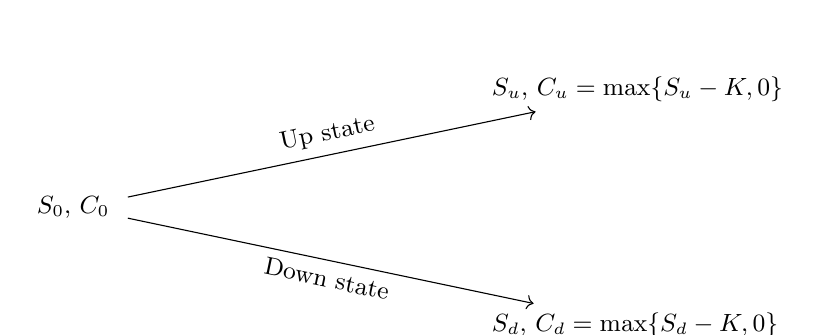
\begin{tikzpicture}[
 =stealth,
 node distance=2.4cm,
 every node/.style={font=\small}
 ]

\node (s0) [align=center] {
\(S_0\),
\(C_0\)
};

\node (su) [right=4.5cm of s0, yshift=1.5cm, align=center] {
\(S_u\),
\(C_u=\max\{S_u-K,0\}\)
};

\node (sd) [right=4.5cm of s0, yshift=-1.5cm, align=center] {
\(S_d\),
\(C_d=\max\{S_d-K,0\}\)
};

\draw[->] (s0) -- node[above, sloped] {Up state} (su);
\draw[->] (s0) -- node[below, sloped] {Down state} (sd);

\end{tikzpicture}

\caption{One-period binomial structure for a call option}
\label{fig:ch18-one-period-binomial}
\end{figure}

A portfolio containing \(\Delta\) shares and a risk-free position \(B\) replicates these payoffs when

\begin{align*}
\Delta S_u+B(1+r)&=C_u,\\
\Delta S_d+B(1+r)&=C_d.
\end{align*}

Solving the two equations gives

\begin{equation}
\Delta
=\frac{C_u-C_d}{S_u-S_d},
\label{eq:ch18-binomial-delta}
\end{equation}

and

\begin{equation}
B
=\frac{C_d-\Delta S_d}{1+r}.
\label{eq:ch18-binomial-bond}
\end{equation}

Under no-arbitrage conditions, the option value equals the current cost of the replicating portfolio:

\begin{equation}
C_0=\Delta S_0+B.
\label{eq:ch18-binomial-value}
\end{equation}

The valuation follows from reproducing the option's state-contingent payoffs rather than from forecasting which state will occur.

In the one-period binomial tree shown in
Figure~\ref{fig:ch18-one-period-binomial}, the initial stock
price $S_0$ can move to either $S_{u}=uS_0$ in the up state
or $S_{d}=dS_0$ in the down state. Let $q$ denote the
risk-neutral probability assigned to the up state,
so that $1-q$ is the probability assigned to the
down state.

Under risk-neutral valuation, the expected future
stock price, discounted at the risk-free rate, must
equal its current price. Thus,

\begin{equation*}
S_0=\frac{quS_0+(1-q)dS_0}{1+r}.
\end{equation*}

Rearranging gives

\begin{equation*}
1+r=qu+(1-q)d.
\end{equation*}

Solving for $q$ gives the risk-neutral probability

\begin{equation}
q=\frac{(1+r)-d}{u-d}.
\label{eq:ch18-binomial-risk-neutral-probability}
\end{equation}

\begin{example}{One-Period Call Option Valuation}{one-period-call-ch18}

A stock sells for RMB~100 and will be either RMB~120 or RMB~80 in one year. The risk-free rate is 5\%, and a call has a strike price of RMB~100. Its payoffs are RMB~20 in the up state and zero in the down state. Hence,

$$
\Delta=\frac{20}{120-80}=0.5,
$$

and

$$
B=\frac{0-0.5\times 80}{1.05}=-38.095.
$$

The call option value is

$$
C_0=0.5\times 100-38.095=11.905.
$$

\end{example}

The same logic extends to successive periods. In a two-period tree, terminal payoffs are determined first and earlier node values are obtained by backward induction.

\begin{figure}[H]
\centering
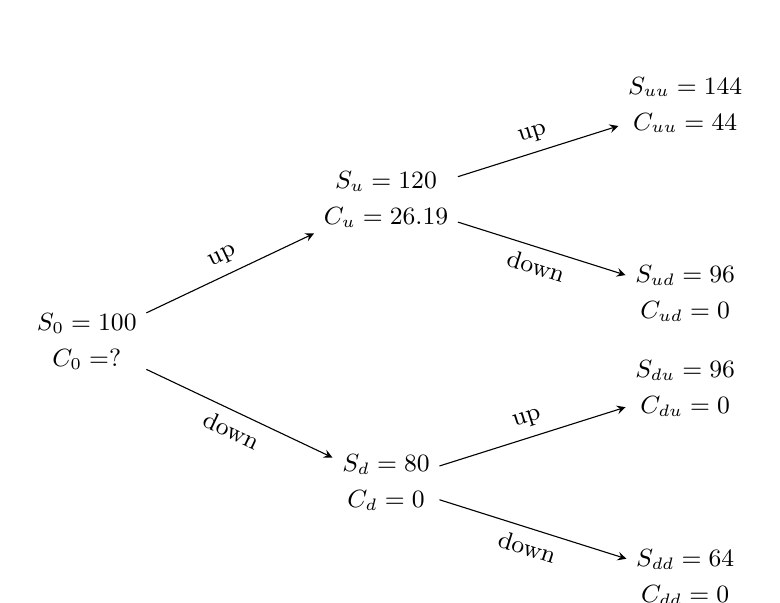
\begin{tikzpicture}[
    >=stealth,
    every node/.style={font=\small},
    level 1/.style={sibling distance=42mm},
    level 2/.style={sibling distance=24mm}
]

\node (S0) at (0,0) [align=center] {$S_0=100$\\[2pt] $C_0=?$};

\node (Su) at (3.8,1.8) [align=center] {$S_u=120$\\[2pt] $C_u=26.19$};
\node (Sd) at (3.8,-1.8) [align=center] {$S_d=80$\\[2pt] $C_d=0$};

\node (Suu) at (7.6,3.0) [align=center] {$S_{uu}=144$\\[2pt] $C_{uu}=44$};
\node (Sud) at (7.6,0.6) [align=center] {$S_{ud}=96$\\[2pt] $C_{ud}=0$};
\node (Sdu) at (7.6,-0.6) [align=center] {$S_{du}=96$\\[2pt] $C_{du}=0$};
\node (Sdd) at (7.6,-3.0) [align=center] {$S_{dd}=64$\\[2pt] $C_{dd}=0$};

\draw[->] (S0) -- node[above,sloped] {up} (Su);
\draw[->] (S0) -- node[below,sloped] {down} (Sd);

\draw[->] (Su) -- node[above,sloped] {up} (Suu);
\draw[->] (Su) -- node[below,sloped] {down} (Sud);

\draw[->] (Sd) -- node[above,sloped] {up} (Sdu);
\draw[->] (Sd) -- node[below,sloped] {down} (Sdd);

\end{tikzpicture}
\caption{Two-period binomial tree for a European call}
\label{fig:ch18-two-period-binomial}
\end{figure}




For a two-period European call, backward induction gives

\begin{equation}
C_u=
\frac{qC_{uu}+(1-q)C_{ud}}{1+r},
\qquad
C_d=
\frac{qC_{du}+(1-q)C_{dd}}{1+r},
\label{eq:ch18-binomial-one-period-backward}
\end{equation}
and

\begin{equation}
C_0=
\frac{qC_u+(1-q)C_d}{1+r}.
\label{eq:ch18-binomial-two-period-backward}
\end{equation}

\begin{example}{Two-Period Call Valuation}{two-period-call-valuation}

Suppose \(S_0=100\), with \(u=1.2\), \(d=0.8\), and a risk-free rate of 5\% per period. A European call option has strike price \(K=100\) and maturity of two periods.

At maturity, the stock prices are \(144\), \(96\), and \(64\), giving call option payoffs of \(44\), \(0\), and \(0\). The risk-neutral probability is

$$
q=\frac{1.05-0.8}{1.2-0.8}=0.625.
$$

At the first-period nodes,

$$
C_u=
\frac{0.625\times 44}{1.05}
=26.19,
\qquad
C_d=0.
$$

Moving back one more period gives

$$
C_0=
\frac{0.625\times 26.19}{1.05}
=15.59.
$$

Thus the multi-period value is obtained by working backward from terminal option payoffs through the tree.

\end{example}

The procedure extends to larger trees. For an option that can be exercised before maturity, the value at each exercise date is obtained by comparing the payoff from immediate exercise with the value of keeping the option alive.

The binomial framework makes replication transparent in discrete states. The same pricing principle can be extended to settings in which the underlying price evolves continuously.


\subsection[Black--Scholes--Merton: Risk-Neutral Pricing Intuition]{Black--Scholes--Merton: Risk-Neutral Pricing Intuition}

In continuous time, the Black--Scholes--Merton framework expresses the same no-arbitrage logic through dynamic replication. For a European call option on a non-dividend-paying stock,

\begin{equation}
C_0
=S_0N(d_1)-Ke^{-rT}N(d_2),
\label{eq:ch18-bsm-call}
\end{equation}
where

\begin{equation}
d_1
=\frac{\ln(S_0/K)+(r+\tfrac{1}{2}\sigma^2)T}{\sigma\sqrt{T}},
\qquad
d_2=d_1-\sigma\sqrt{T},
\label{eq:ch18-bsm-d1d2}
\end{equation}
and \(N(\cdot)\) is the standard normal cumulative distribution function. The corresponding European put option value is

\begin{equation}
P_0
=Ke^{-rT}N(-d_2)-S_0N(-d_1).
\label{eq:ch18-bsm-put}
\end{equation}

The pricing mechanism rests on a dynamically adjusted position in the stock and risk-free financing. As the stock price changes, the hedge is rebalanced to reproduce the option's local exposure. Under the model assumptions, no-arbitrage links the option value to the cost of this replicating strategy.

The same result can be represented through risk-neutral valuation. For pricing purposes, the stock's expected return is replaced by the risk-free rate, and the option value is obtained from the discounted expected payoff under the risk-neutral measure. This representation is consistent with replication and does not require the risk-neutral distribution to describe actual future outcomes.

The benchmark model assumes frictionless trading, continuous rebalancing, a continuous stock-price process with constant volatility, and a constant risk-free rate in its basic form. Actual markets may involve transaction costs, discrete trading, price jumps, liquidity constraints, and changing volatility, so the model is best viewed as a benchmark for valuation.

Observed option prices can also be expressed through implied volatility, defined as the value of \(\sigma\) that makes the model price equal to the market price. Once an option value is expressed as a function of its underlying inputs, the same framework can also be used to measure how that value responds to changes in those inputs.


\begin{tcolorbox}[
enhanced,
breakable,
colback=white,
colframe=FinanceBlue,
boxrule=0.7pt,
sharp corners,
borderline west={2.2pt}{0pt}{FinanceBlue},
title=\textbf{Financial Perspective: A Pricing Model Is Not a Forecast},
coltitle=white,
colbacktitle=FinanceBlue,
fonttitle=\bfseries,
before skip=1.2em,
after skip=1.2em
]

Risk-neutral pricing uses traded prices and no-arbitrage conditions to value contingent claims. The resulting risk-neutral distribution need not coincide with investors' beliefs about actual future outcomes.

\end{tcolorbox}

\subsection{Put--Call Parity and No-Arbitrage Consistency}

European call and put options written on the same underlying
asset, with the same strike price and expiration date, are
linked by a no-arbitrage relationship known as put--call
parity. The relationship follows from the equivalence of
two portfolios that generate identical payoffs at maturity.

Consider two portfolios. Portfolio A consists of a European
call option and a risk-free zero-coupon bond with face value
$K$. Portfolio B consists of a European put option and one
unit of the underlying asset. Their values at maturity are

\begin{equation*}
\begin{aligned}
W_A(T)&=\max\{S_T-K,0\}+K,\\
W_B(T)&=\max\{K-S_T,0\}+S_T.
\end{aligned}
\end{equation*}

For either $S_T\geq K$ or $S_T<K$, the two portfolios produce
the same terminal payoff:

\begin{equation*}
W_A(T)=W_B(T)=\max\{S_T,K\}.
\end{equation*}

Under no-arbitrage conditions, portfolios with identical
future payoffs must have the same current value. Let $C_0$
and $P_0$ denote the current prices of the call and put
options, respectively, and let $D(0,T)$ denote the
risk-free discount factor to the expiration date. Put--call
parity is therefore

\begin{equation}
C_0+KD(0,T)=P_0+S_0.
\label{eq:ch18-put-call-parity}
\end{equation}

Equivalently,

\begin{equation}
C_0-P_0=S_0-KD(0,T).
\end{equation}

The relationship shows that the difference between call
and put prices is determined by the underlying asset price
and the present value of the strike price. If the two sides
of equation~\eqref{eq:ch18-put-call-parity} differ, an
investor may construct offsetting positions to exploit
the pricing discrepancy.

Put--call parity provides a consistency condition for
European option prices rather than a separate pricing
model. It also illustrates how options, the underlying
asset, and risk-free borrowing or lending can be combined
to construct equivalent financial positions.

\subsection{Option Sensitivities and Dynamic Hedging}

The local responses of option value to changes in market inputs are summarized by the Greeks. Delta measures sensitivity to the underlying price,

\begin{equation}
\Delta=\frac{\partial V}{\partial S},
\label{eq:ch18-delta}
\end{equation}
while gamma measures how delta changes as the underlying price changes,

\begin{equation}
\Gamma=\frac{\partial^2 V}{\partial S^2}.
\label{eq:ch18-gamma}
\end{equation}


For a small change in the underlying asset price, the
change in option value can be approximated by

\begin{equation}
\Delta V
\approx
\frac{\partial V}{\partial S}\times\Delta S
+
\frac{1}{2}\frac{\partial^2 V}{\partial S^2}\times(\Delta S)^2.
\label{eq:ch18-delta-gamma}
\end{equation}

Delta captures the local slope of the option-value function,
while gamma captures its curvature. Standard long calls and
puts typically have positive gamma, so their deltas change
as the underlying price moves. Other Greeks describe
sensitivity to additional pricing inputs. The main option
Greeks and their corresponding sensitivities are summarized
in Table~\ref{tab:ch18-option-greeks}.

\begin{table}[H]
\centering
\caption{Selected option sensitivities}
\label{tab:ch18-option-greeks}
\begin{tabularx}{\textwidth}{@{}p{2.0cm}p{3.0cm}Y@{}}
\toprule
\textbf{Greek} & \textbf{Definition} & \textbf{Interpretation} \\
\midrule
Delta & \(\partial V/\partial S\) & Sensitivity to the underlying price \\
Gamma & \(\partial^2V/\partial S^2\) & Change in delta as the underlying price changes \\
Vega & \(\partial V/\partial \sigma\) & Sensitivity to volatility \\
Theta & \(-\partial V/\partial \tau\) & Sensitivity to the passage of time, where \(\tau\) is time to maturity \\
Rho & \(\partial V/\partial r\) & Sensitivity to the interest rate \\
\bottomrule
\end{tabularx}
\end{table}

These sensitivities provide the basis for dynamic hedging. A dealer who is short calls may buy the underlying asset to offset the position's current delta. As the underlying price changes, the option's delta also changes, so the hedge may need to be rebalanced.

Delta hedging is local rather than permanent. Discrete trading, price jumps, transaction costs, liquidity constraints, changing volatility, and model error can leave residual exposure. Greeks describe how option value responds to market changes, but they do not imply that all risk can be removed.

The need for rebalancing follows from the nonlinear structure of option value. A linear derivative has a relatively stable sensitivity to the underlying, whereas an option's sensitivity changes with market conditions.



\section{Embedded Optionality in Financial Claims}

The same option logic can appear inside securities that are not traded as standalone options. Bonds, mortgages, and structured securities may contain contractual rights that alter the timing, amount, or allocation of future cash flows when specified conditions are met.

\subsection{Convertible Bonds: Equity Options in Debt Contracts}

A convertible bond combines a debt claim with the investor's right to convert the bond into equity under specified terms. The debt component provides contractual payments, while the conversion right links part of the bond's value to the issuer's share price.

If a bond with face value \(F\) can be converted into \(m\) shares, its conversion value at time \(t\) is

\begin{equation}
CV_t=mS_t,
\label{eq:ch18-conversion-value}
\end{equation}
where \(S_t\) is the share price. Under a fixed conversion ratio, the corresponding conversion price is

\begin{equation}
K_c=\frac{F}{m}.
\label{eq:ch18-conversion-price}
\end{equation}

As the share price rises, the conversion value increases. Conversion becomes more attractive when the value of the shares received becomes large relative to the value of retaining the bond. Remaining coupon payments, redemption value, call provisions, and other contract terms can affect this comparison.

From a valuation perspective, a convertible bond combines
the value of a straight bond with the value of the
conversion option:

\begin{equation}
V_{\mathrm{convertible}}
\approx
V_{\mathrm{straight\ bond}}
+
V_{\mathrm{conversion\ option}}.
\label{eq:ch18-convertible-decomposition}
\end{equation}

This decomposition distinguishes the debt component from
the equity-linked conversion option. The conversion
option may allow the issuer to offer a lower coupon than
on otherwise comparable straight debt, since investors
receive potential gains from participating in the
issuer's equity appreciation.

\begin{example}{Conversion Value}{convertible-bond-example}

A convertible bond has face value RMB~1,000 and can be converted into 20 shares. The conversion price is

$$
K_c=\frac{1{,}000}{20}=50.
$$

If the share price is RMB~40, the conversion value is RMB~800. If the share price rises to RMB~65, the conversion value becomes

$$
CV_t=20\times 65=1{,}300.
$$

The higher share price increases the value of the conversion right. Immediate conversion may still be unattractive if retaining the bond provides greater value through coupons, redemption value, or other contractual features.

\end{example}

The decomposition becomes less exact when credit risk and other contractual features interact. Changes in firm value can affect both the debt component and the conversion right, while issuer call provisions or conversion adjustments can further alter the bond's value.

\subsection[Callable and Puttable Bonds: Issuer and Investor Options]{Callable and Puttable Bonds: Issuer and Investor Options}

Whereas conversion rights can change the form of a financial claim, call and put provisions can change the timing of its repayment. A callable bond gives the issuer the right to redeem the bond before maturity under specified terms, while a puttable bond gives the investor the right to require early repayment.

For a callable bond, the investor has effectively granted
the issuer an embedded call right. This right reduces the
bond's value relative to an otherwise comparable straight
bond, since the issuer may redeem the bond when doing so
is advantageous to the issuer but potentially unfavorable
to the investor.

The call becomes more valuable when refinancing on new terms becomes attractive relative to maintaining the existing debt. If the issuer exercises, the investor receives the contractual call price and gives up the remaining cash flows of the original bond. The call provision can therefore limit the bond's price appreciation when market yields fall.

A puttable bond grants the investor the right to require
the issuer to redeem the bond before maturity at a
specified price. This right increases the bond's value
relative to an otherwise comparable straight bond,
because it provides protection against adverse changes
in market conditions, particularly rising interest rates.

The put becomes more valuable when continued holding becomes less attractive relative to exercising the repayment right. Higher market yields, weaker credit quality, or other relevant changes can increase the value of this protection, subject to the contract terms.

These embedded options also change interest-rate exposure. A noncallable bond generally rises in value as yields fall. For a callable bond, further appreciation may become limited as exercise of the issuer's call becomes more attractive, producing negative convexity over part of the price--yield relation.

Contract terms determine how strongly these effects operate. call prices, call-protection periods, notice requirements, make-whole provisions, investor put dates, and related features affect both the exercise decision and the value of the embedded option.

\subsection{Mortgage Prepayment and Refinancing Options}

The issuer's call right in a callable bond has an economic counterpart in a mortgage: the borrower may repay the loan before its scheduled maturity, creating an embedded prepayment option.

For a fixed-rate mortgage, this option becomes more valuable when market mortgage rates fall sufficiently to make refinancing attractive. The borrower can repay the existing loan and replace it with lower-cost financing, subject to refinancing costs, qualification requirements, contractual restrictions, and other frictions.

From the lender's or mortgage-backed securities investor's perspective, prepayment changes the timing of expected cash flows. When rates fall, principal may be returned earlier, limiting price appreciation and exposing the investor to reinvestment at lower rates. When rates rise, refinancing incentives weaken and the expected life of the mortgage may extend.

This embedded option can contribute to negative convexity
in mortgage-related claims. Price appreciation may become
more limited as rates decline, while duration may increase
as rates rise. These effects complicate the valuation and
risk management of mortgage-related assets.

Prepayment behavior also depends on borrower-specific and
contractual factors, including mobility, housing turnover,
credit conditions, loan seasoning, refinancing costs,
loan-to-value ratios, and contract terms. Mortgage valuation therefore reflects both interest-rate movements and uncertainty about the exercise of the borrower's
prepayment right.


\subsection{Structured Notes and Embedded Options}

Mortgage prepayment illustrates optionality arising from rights embedded in a conventional contract. Structured notes take the logic a step further by deliberately combining debt and derivative components to create specified state-dependent cash flows. These structures may provide principal protection, equity participation, enhanced coupons, or contingent repayment.

A principal-protected note combines a debt component that
provides repayment of face value at maturity with an
option component that provides participation in equity
market gains. Its value can be represented approximately
as the sum of these two components:

\begin{equation}
V_{\mathrm{note}}
\approx
V_{\mathrm{zero\text{-}coupon\ bond}}
+
V_{\mathrm{call\ component}}.
\label{eq:ch18-principal-protected-note}
\end{equation}

The bond component supports the promised principal payment, while the option component creates participation in favorable equity states. The resulting participation rate depends on the value allocated to the option and on its contractual terms.

Other structures redistribute risk differently. A reverse convertible, for example, may offer a higher coupon while exposing the investor to losses when the underlying asset performs poorly. Economically, part of the additional coupon compensates the investor for accepting downside exposure.

\begin{table}[H]
\centering
\caption{Illustrative structured-note decompositions}
\label{tab:ch18-structured-notes}
\begin{tabularx}{\textwidth}{@{}p{3.5cm}YY@{}}
\toprule
\textbf{Structure} &
\textbf{Illustrative building blocks} &
\textbf{Main economic feature} \\
\midrule
Principal-protected note &
Zero-coupon bond plus long call-type exposure &
Principal repayment with conditional participation in favorable underlying performance \\
Equity-linked participation note &
Debt claim plus option exposure &
Return or redemption linked to equity performance \\
Reverse convertible &
Debt claim plus short put-type exposure &
Higher coupon combined with investor exposure to downside states \\
\bottomrule
\end{tabularx}
\end{table}

More complex notes may contain barriers, digital payoffs, caps, multiple underlyings, or combinations of options. These features can make the economic exposure less transparent than the product label or quoted coupon suggests.

Issuer credit risk remains distinct from the market protection created by the embedded derivatives. A note described as principal protected generally remains a claim on the issuer unless the principal payment is separately secured or guaranteed. Protection against adverse market movements does not by itself eliminate exposure to issuer default.

\begin{example}{Reading a Reverse Convertible Economically}{reverse-convertible-example}

An investor purchases a one-year note with face value RMB~100 and an enhanced coupon. If the referenced stock finishes above the contractual strike, the investor receives the face value at maturity. If the stock falls sufficiently below the strike, the redemption value declines according to the contract's conversion rule.

The additional coupon compensates the investor, in part, for accepting downside exposure in the underlying asset as well as the issuer's credit risk.

\end{example}

Structured-note analysis therefore begins with the cash-flow structure rather than the product label. Decomposition helps identify which states create gains or losses, which party bears the embedded option exposure, and how those contingent cash flows contribute to value.




%========================================================
% Summary
%========================================================

\TailModule{summary}{Summary}

Options differ from linear derivatives through an asymmetric allocation of rights and obligations. A call option gives the holder the right to buy at the strike price, while a put option gives the right to sell. The holder may decline to exercise, while the writer accepts a contingent obligation in exchange for the premium.

This asymmetry allows options to reshape exposures across future states. Puts can establish price floors, calls can limit purchase costs, and option selling can exchange selected future exposure for premium income. Option value depends on the underlying price, strike, time, volatility, interest rates, and relevant cash distributions. Replication, risk-neutral valuation, and option sensitivities provide the main tools for understanding valuation and dynamic hedging.

Optionality also appears within broader financial claims. Convertible, callable, and puttable bonds, prepayable mortgages, and structured notes allocate decision rights that alter future cash flows. Identifying who holds the right, when exercise becomes attractive, and how cash flows change across states helps reveal the economic structure of these instruments.



%========================================================
% Key Terms
%========================================================

\TailModule{keyterms}{Key Terms}

Call option; put option; strike price; option premium; exercise;
European option; American option; intrinsic value; time value; moneyness;
protective put; put--call parity; binomial model; risk-neutral valuation;
Black--Scholes--Merton model; implied volatility; delta; gamma;
dynamic hedging; embedded option; convertible bond; callable bond;
prepayment option; structured note.



%========================================================
% Financial AI Lab
%========================================================

\TailModule{aiprompt}{Financial AI Lab}

\textbf{Lab: Audit an Option Valuation and Embedded-Option Decomposition}

Ask an AI system to value a European call option and analyze
a structured note linked to the same underlying stock.
Provide the stock price, strike price, maturity, risk-free
rate, volatility, and dividend yield, if relevant. For the
structured note, also specify its face value, participation
rate, maturity payment terms, payoff limits, and any
additional contractual features. Require the AI system
to state its assumptions and show the main calculation
steps.

Audit the answer in five stages.

\begin{enumerate}

\item \textbf{Check the payoff structure.}

Write the call option payoff directly from the contract
and verify it for several terminal stock prices. Keep
the option premium separate from the maturity payoff
and the resulting profit.

\item \textbf{Check the valuation logic.}

Examine how the option value responds to changes in the
stock price, strike, volatility, maturity, interest rate,
and dividend yield. Use a one-period binomial model to
verify the replication logic, and a multi-period binomial
model to compare the valuation with the
Black--Scholes--Merton model.

\item \textbf{Check no-arbitrage consistency.}

Use put--call parity to examine whether the call and put
prices are consistent with the underlying asset price,
strike price, and discount factor. Identify the assumptions
required for the parity relationship to hold.

\item \textbf{Distinguish pricing inputs from forecasts.}

If implied volatility is reported, explain how it is
obtained from the market price and why it need not equal
future realized volatility. Check that risk-neutral
valuation is used as a pricing framework rather than
as a direct forecast of future outcomes.

\item \textbf{Decompose the structured note.}

Identify the debt component and embedded option positions.
Determine who holds each option, which states create
gains or losses for the investor, and how the participation
rate and any payoff limits affect the investor's return.
Examine whether issuer credit risk remains when the note
provides protection against market losses.

\end{enumerate}


%========================================================
% Applied Problems
%========================================================

\TailModule{appprobs}{Applied Problems}

\begin{enumerate}

\item \textbf{Call and put option payoffs.}

A stock is currently priced at RMB~100. Consider a call and a put option, each with strike price RMB~105 and maturity in six months.

\begin{enumerate}

\item Calculate the call option and put option payoffs when the stock price at maturity is RMB~80, RMB~105, and RMB~130.

\item If the call option premium is RMB~6 and the put option premium is RMB~8, calculate the corresponding profits at maturity, ignoring financing of the premiums.

\item Explain why payoff and profit are different measures.

\end{enumerate}

\item \textbf{Protective put and covered call.}

An investor owns one share. Consider two alternative option strategies.

\begin{enumerate}

\item The investor buys a put option with strike price RMB~90. Write the combined maturity payoff, excluding the premium, and calculate it for stock prices of RMB~60, RMB~90, and RMB~130.

\item The investor instead sells a call option with strike price RMB~115. Write the combined maturity payoff, excluding the premium received, and calculate it for the same stock prices.

\item Compare how the two strategies redistribute exposure across future price states.

\end{enumerate}

\item \textbf{Put--call parity.}

A non-dividend-paying stock sells for RMB~50. A one-year European call option with strike price RMB~52 is priced at RMB~5.20. The continuously compounded risk-free rate is 3\%.

\begin{enumerate}

\item Use put--call parity to calculate the price of the corresponding European put.

\item Construct the two portfolios implied by put--call parity and compare their maturity payoffs when the stock price is RMB~40 and RMB~65.

\item Explain how a material violation of parity could create an arbitrage opportunity under the assumed market conditions.

\end{enumerate}

\item \textbf{One-period binomial valuation.}

A stock sells for RMB~80. In one period, its price will be either RMB~96 or RMB~68. The one-period risk-free rate is 4\%. A call option has strike price RMB~82.

\begin{enumerate}

\item Calculate the call option payoff in each state.

\item Find the replicating stock position \(\Delta\) and risk-free position \(B\).

\item Calculate the current call option value from the replicating portfolio.

\item Calculate the risk-neutral probability and verify the same option value.

\item Explain why the valuation does not require a forecast of the actual probability of the up state.

\end{enumerate}

\item \textbf{Delta and dynamic hedging.}

A dealer is short 5,000 call options. Each option currently has \(\Delta=0.35\).

\begin{enumerate}

\item Calculate the delta of the option position.

\item Calculate the number of underlying units required for a local delta-neutral hedge, ignoring contract multipliers.

\item Suppose the call option $\Delta$ rises to \(0.50\). Calculate the required hedge adjustment.

\item Explain how gamma creates the need for rebalancing and why a delta hedge may remain imperfect in practice.

\end{enumerate}

\item \textbf{Convertible bond optionality.}

A convertible bond has face value RMB~1,000 and can be converted into 25 shares.

\begin{enumerate}
\item Calculate the conversion price.

\item Calculate the conversion value when the share price is RMB~30, RMB~40, and RMB~55.

\item Explain how the debt component and conversion right jointly affect the value of the convertible bond.

\item Identify two contractual or credit-related features that could complicate the simple decomposition into straight debt plus a conversion option.

\end{enumerate}

\item \textbf{Callable bonds and mortgage prepayment.}

Callable bonds and prepayable mortgages both contain rights that can shorten the life of a debt claim.

\begin{enumerate}

\item Explain why a decline in market interest rates can increase the value of an issuer's call option on a callable bond.

\item Explain how the call provision can limit the bond's price appreciation and contribute to negative convexity.

\item A borrower has a fixed-rate mortgage at 5.5\% and market mortgage rates fall to 3.8\%. Explain why the prepayment option becomes more valuable.

\item Identify three frictions that may prevent immediate refinancing and explain how prepayment uncertainty changes the investor's interest-rate exposure.

\end{enumerate}

\item \textbf{Structured-note decomposition.}

A one-year note pays a coupon above the yield on comparable straight debt. It returns face value at maturity unless an equity index falls below a specified threshold, in which case the investor bears part of the index loss.

\begin{enumerate}

\item Identify the debt component and the put-like downside exposure embedded in the note.

\item Explain why the higher coupon should be evaluated together with the contingent downside payoff.

\item Explain how greater volatility may affect the value of the embedded option exposure.

\item Explain why issuer credit risk remains even when the note provides some contractual protection against market losses.

\end{enumerate}

\end{enumerate}



%========================================================
% Further Reading
%========================================================

\TailModule{furtherread}{Further Reading}

\begin{itemize}

\item Black, Fischer, and Myron Scholes (1973),
``The Pricing of Options and Corporate Liabilities,''
\emph{Journal of Political Economy}, 81(3), 637--654.

\item Merton, Robert C. (1973),
``Theory of Rational Option Pricing,''
\emph{The Bell Journal of Economics and Management Science}, 4(1), 141--183.

\item Cox, John C., Stephen A. Ross, and Mark Rubinstein (1979),
``Option Pricing: A Simplified Approach,''
\emph{Journal of Financial Economics}, 7(3), 229--263.

\item Brennan, Michael J., and Eduardo S. Schwartz (1977),
``Convertible Bonds: Valuation and Optimal Strategies for call and Conversion,''
\emph{The Journal of Finance}, 32(5), 1699--1715.

\item Dunn, Kenneth B., and Chester S. Spatt (2005),
``The Effect of Refinancing Costs and Market Imperfections on the Optimal call Strategy and the Pricing of Debt Contracts,''

\emph{Real Estate Economics}, 33(4), 595--617.

\end{itemize}


\ChapterTail{summary,keyterms,aiprompt,appprobs,furtherread}
\chapter{Credit Risk, Default, and Risk Transfer}
\label{chap:Credit_Risk_Default_and_Risk_Transfer}

\begin{openingcase}{No Default Occurred---Why Did the Credit Position Lose Value?}

An institutional investor holds a five-year corporate bond. The issuer has made every scheduled payment on time, and none of the bond's contractual cash flows has changed. Yet weaker earnings and rising leverage lead investors to demand greater compensation for bearing the issuer's credit risk. The bond price falls, its credit spread widens, and the investor records a loss before any payment has been missed.

The same deterioration appears in the market for credit protection. Even though the issuer has not missed a payment, the premium required to insure against its default rises. The bond is still performing, yet both its market price and the price of protection now reflect a weaker credit position.

\end{openingcase}


\begin{tcolorbox}[
  enhanced,
  colback=FinanceBlue!6,
  colframe=FinanceBlue,
  boxrule=0.6pt,
  sharp corners,
  left=8pt,
  right=8pt,
  top=7pt,
  bottom=7pt,
  before skip=1em,
  after skip=1.6em,
  title=\textbf{Core Questions},
  coltitle=white,
  colbacktitle=FinanceBlue,
  fonttitle=\bfseries,
  attach boxed title to top left={xshift=6pt,yshift=-2mm},
  boxed title style={
    boxrule=0pt,
    sharp corners,
    left=5pt,
    right=5pt,
    top=2pt,
    bottom=2pt
  }
]
\begin{enumerate}[
  leftmargin=*,
  label=\textcolor{FinanceBlue}{\textbf{\arabic*.}},
  itemsep=0.55em,
  topsep=0.2em
]


\item How can credit risk be decomposed into default likelihood, loss severity, and exposure at the time of default?

\item How do credit default swaps and credit indices transfer default risk without necessarily transferring the underlying loan or bond?

\item What information is contained in bond spreads, CDS spreads, and credit ratings, and why should these signals not be interpreted as direct measures of the same object?


\end{enumerate}
\end{tcolorbox}


\section{Credit Risk Fundamentals and Default Losses}

Credit risk can be analyzed through three basic components: the likelihood of default, the loss that would follow if default occurs, and the amount exposed at that time. These components can be summarized by

$$
EL=PD\times LGD\times EAD.
$$

Credit risk can change before any payment is missed. An issuer may continue to meet every contractual obligation while its expected repayment capacity deteriorates. Such deterioration can reduce the market value of a loan or bond, widen its credit spread, raise the cost of credit protection, and alter financing conditions. Default is one possible outcome of this process, not the only economically relevant manifestation of credit risk.


\subsection{Probability of Default and Credit Deterioration}

The first component of expected credit loss is the likelihood of default. This likelihood is defined over a stated horizon and can change as the obligor's financial condition evolves. A one-year default probability and a five-year cumulative default probability therefore describe different exposures to credit risk.

Let \(PD(0,T)\) denote the cumulative probability that default occurs between today and date \(T\). The corresponding survival probability is

\begin{equation*}
S(0,T)=1-PD(0,T).
\label{eq:ch19-survival-probability}
\end{equation*}

Survival means that the obligor has not entered the defined default state by date \(T\). The relevant definition of default depends on the application. Bank credit models, bond contracts, and credit derivatives may use closely related but not identical event definitions.

Let \(\lambda(t)\) denote the conditional default intensity at time \(t\), given survival to that time. In a continuous-time representation, the survival probability is

\[
S(0,T)
=\exp\left(
-\int_0^T \lambda(u)\,du
\right).
\]

Since default and survival are complementary events, the cumulative probability of default is one minus the survival probability. If the hazard rate is constant at \(\lambda\),

\begin{equation}
PD(0,T)=1-e^{-\lambda T}.
\end{equation}

\begin{example}{From Annual Hazard to Cumulative Default Probability}{hazard-pd}

Suppose a simplified model uses a constant annual hazard rate of 2\%. The three-year survival probability is

$$
S(0,3)=e^{-0.02 \times 3}\approx0.9418.
$$

The corresponding cumulative default probability is

$$
PD(0,3)=1-0.9418\approx5.82\%.
$$

The annual hazard rate is not the same as the cumulative probability of default over three years. The latter depends on both the horizon and survival through time.

\end{example}

Default probability is not fixed over the life of a credit exposure. Lower profitability, rising leverage, weaker liquidity, declining debt-service capacity, adverse industry conditions, or reduced access to refinancing can weaken an obligor's expected ability to meet future payments. Market participants may then assign a higher probability to future default even while current payments continue to be made.

Changes in credit quality can also be represented through credit migration. An obligor may move to a stronger or weaker rating category, remain in the same category, or enter default. A transition matrix summarizes estimated movements across credit states over a chosen horizon. Such estimates are useful in portfolio analysis, although observed transition frequencies can vary across business cycles, sectors, and institutional environments.

Default probabilities can be estimated from historical default experience, borrower fundamentals, structural models, reduced-form models, market prices, or combinations of these sources. The resulting measures need not coincide. Historical and model-based estimates may be designed to capture real-world default frequencies, while market-implied measures can also reflect risk premia, liquidity conditions, and pricing conventions.

Default likelihood determines only whether a loss event may occur. The size of the loss, conditional on default, depends on recovery and the structure of the underlying claim.

\subsection{Loss Given Default, Recovery, and Collateral}

Assessing loss conditional on default involves two key quantities: exposure at default (EAD) and the recovery rate (RR). Exposure at default (EAD) is the amount of credit exposure outstanding when the obligor defaults. It may include outstanding principal, accrued interest, and other relevant amounts owed at the time of default. The recovery rate measures the proportion of EAD recovered after default:

\begin{equation}
RR=\frac{R}{EAD},
\label{eq:ch19-recovery-rate}
\end{equation}
where \(R\) is the value recovered after default, net of
relevant recovery costs.

Loss given default (LGD) measures the proportion of EAD
that is not recovered. It therefore captures the severity
of loss rather than the likelihood of default:

\begin{equation}
LGD=1-RR.
\label{eq:ch19-lgd}
\end{equation}

These expressions summarize a recovery process that may
extend well beyond the default date. Recoveries can
involve delayed payments, restructuring, legal expenses,
collateral liquidation costs, and uncertain timing. A
recovery received several years after default has a lower
economic value than the same nominal amount received
immediately, so expected recovery may need to be evaluated
on a present-value basis.

Recovery depends on both the value available in distress and the contractual position of the claim. Seniority determines priority over available assets, while collateral, guarantees, and structural subordination affect the creditor's access to particular sources of repayment. Insolvency procedures, industry conditions, and the broader economic environment can also influence the value available for distribution.

Collateral affects LGD through its contribution to recovery. Let \(V_C\) denote collateral value before liquidation adjustments. The effective value of collateral, after applying a haircut, can be expressed as:

\begin{equation}
V_C^{\mathrm{eff}}
=(1-h)V_C,
\label{eq:ch19-effective-collateral}
\end{equation}
where \(h\) represents valuation haircuts, liquidation costs, and other reductions in realizable value.

The protection provided by collateral depends not only on its initial value but also on how that value changes as the borrower's condition deteriorates. If collateral values tend to fall when default risk rises, expected recovery may weaken at the same time that default becomes more likely. This interaction can be important in real-estate lending, commodity finance, and other secured exposures exposed to common economic conditions.

Two claims with similar default probabilities can therefore generate different expected losses when they differ in seniority, collateral quality, guarantees, or recovery prospects.

\begin{example}{Same Default Probability, Different Loss Severity}{lgd-example}

Two one-year exposures are each RMB~10 million and each has a default probability of 2\%. Exposure A has an expected recovery rate of 70\%, while Exposure B has an expected recovery rate of 30\%.

Their expected losses are

\begin{align*}
EL_A
&=
0.02\times(1-0.70)\times10
=
\text{RMB~}0.06 \text{ million},\\
EL_B
&=
0.02\times(1-0.30)\times10
=
\text{RMB~}0.14 \text{ million}.
\end{align*}


The difference arises from loss severity rather than default likelihood.

\end{example}

LGD determines the fraction of exposure lost after default. Expected loss also depends on the amount outstanding when default occurs, which need not equal the current exposure.


\subsection{Exposure at Default}

The amount exposed at default need not equal the amount observed today. Its evolution depends on the structure of the claim, contractual commitments, borrower behavior, and, for market-valued positions, changes in market prices.

For a fully funded term loan, EAD is generally linked to the outstanding principal and accrued amounts at the time of default. In an amortizing loan, exposure tends to decline as principal is repaid. Prepayments, additional advances, or changes in the repayment schedule can alter this path.

Committed credit facilities introduce greater uncertainty. A borrower may draw unused capacity as alternative funding becomes less available. Let \(D\) denote the amount already drawn and \(U\) the undrawn commitment at the measurement date. The credit conversion factor (CCF), denoted by \(c\), represents the expected proportion of the undrawn amount that will be drawn before default. EAD can then be estimated as

\begin{equation}
EAD=D+cU.
\label{eq:ch19-ead-credit-line}
\end{equation}

The conversion factor is an estimate rather than a contractual outcome. It can vary with borrower characteristics, facility design, economic conditions, and the degree of credit deterioration. The exposure of a revolving facility is therefore partly contractual and partly behavioral.

Market-valued claims follow a different exposure path. For derivatives, the amount at risk changes with market value rather than with a fixed principal balance. At default, the relevant exposure is generally the positive replacement value remaining after applicable netting and collateral. Before default, exposure estimates may also allow for possible future changes in market value over the relevant horizon.

EAD can also move with credit quality. A borrower under stress may draw more heavily on a committed facility as default risk rises. In derivatives, adverse market movements can increase exposure while weakening the counterparty. Such dependence means that \(PD\), \(LGD\), and \(EAD\) need not behave as independent and fixed quantities.

\begin{table}[H]

\centering

\caption{Illustrative Sources of Exposure at Default}

\label{tab:ch19-ead-exposures}

\begin{tabularx}{\textwidth}{@{}p{3.5cm}YY@{}}

\toprule

\textbf{Exposure} &
\textbf{Main EAD Component} &
\textbf{Source of Uncertainty} \\

\midrule

Term loan &
Outstanding principal and accrued amounts &
Repayment, prepayment, and changes in outstanding balance \\

Revolving credit line &
Drawn balance plus part of the undrawn commitment &
Drawdown behavior before default \\

Bond &
Outstanding contractual claim &
Accrued amounts and timing of default \\

Derivative &
Positive net replacement exposure &
Market movements, netting, collateral, and close-out timing \\

\bottomrule

\end{tabularx}

\end{table}


EAD determines the amount exposed when default occurs. Together with default likelihood and loss severity, it provides the final component needed to evaluate expected credit loss.

\subsection{Expected and Unexpected Credit Loss}

Once default likelihood, loss severity, and exposure at default have been identified, expected credit loss can be summarized as

\begin{equation}
EL=PD\times LGD\times EAD.
\label{eq:ch19-expected-loss}
\end{equation}

The expression separates expected loss into three distinct sources: the probability that default occurs, the fraction of exposure lost conditional on default, and the amount exposed at that time. For a portfolio with exposures indexed by \(i\), expected loss can be aggregated as

\begin{equation}
EL_{\mathrm{portfolio}}
=\sum_{i=1}^{n}
PD_i\times LGD_i\times EAD_i.
\label{eq:ch19-portfolio-el}
\end{equation}

Expected loss describes the average loss across possible future outcomes. Actual losses can deviate substantially from this average. The uncertainty around expected loss introduces a second dimension of credit risk: unexpected loss. 

Let \(L\) denote random portfolio credit loss. Unexpected loss (UL) is commonly measured by the standard deviation of the loss distribution:

\begin{equation}
UL=\sqrt{\operatorname{Var}(L)}.
\label{eq:ch19-unexpected-loss}
\end{equation}

Other measures focus on high percentiles of the loss distribution or on losses beyond a selected percentile. Although these measures differ in construction, they address the same underlying issue: portfolios with the same expected loss can still have very different distributions of adverse outcomes.

This distinction becomes especially important at the portfolio level. Diversification can reduce loss variability when individual defaults do not move closely together. Credit exposures, however, are often affected by common interest rates, commodity prices, property markets, industry conditions, and macroeconomic shocks. These shared factors create default dependence and can limit the reduction in risk achieved through diversification.

\begin{example}{Same Expected Loss, Different Concentration}{concentration-example}

Portfolio A contains one RMB~100 million loan with a 1\% default probability and an LGD of 50\%. Its expected loss is

$$
0.01\times 0.5\times 100
=
\text{RMB~} 0.5\text{ million}.
$$

Portfolio B contains 100 loans of RMB~1 million each with the same individual PD and LGD. Its expected loss is also RMB~0.5 million.

The two portfolios therefore have the same expected loss, but their loss distributions need not be the same. If defaults among the smaller loans are not closely synchronized, Portfolio B can have lower concentration risk. Common shocks can still generate joint losses and weaken the benefits of diversification.

\end{example}

Expected and unexpected loss therefore capture different dimensions of credit risk. Expected loss concerns the average level of loss associated with an exposure or portfolio, while unexpected loss concerns the dispersion and tail of possible losses around that average. Pricing, provisioning, capital, concentration limits, diversification, and risk-transfer decisions can respond differently to these two dimensions.


\section[Credit Risk Transfer and Credit Derivatives]{Credit Risk Transfer and Credit \\Derivatives}

Once credit risk has been measured, the next question is who bears it. The holder of a loan or bond need not retain all of the associated credit exposure. A separate contract can transfer part of that risk without transferring the underlying claim.

Credit derivatives provide such a mechanism. A lender can keep the loan while transferring part of the loss associated with a specified credit event, while another investor can assume credit exposure without owning the underlying asset. Credit risk is therefore reallocated across parties rather than eliminated.


\subsection[Credit Default Swaps: Contract Design and Payoffs]{Credit Default Swaps: Contract Design and \\Payoffs}

A credit default swap (CDS) implements this transfer through two contractual legs. The protection buyer makes periodic premium payments, while the protection seller makes a contingent payment if a specified credit event occurs with respect to the reference entity or obligation.

Let \(N\) denote the CDS notional amount and \(s\) the annualized CDS spread. If premium payments are scheduled at dates \(t_1,\ldots,t_m\), the premium payment due at date \(t_i\) is \(sN\Delta_i\), where \(\Delta_i\) is the year fraction for the corresponding premium period.

If a credit event specified in the CDS contract occurs, the protection seller makes a payment to the protection buyer. Under cash settlement, the payment is based on the difference between the CDS notional amount and the post-credit-event value of the reference obligation. Let \(P_{\mathrm{final}}\) denote the final settlement price expressed as a proportion of face value. The protection payment can be represented as

\begin{equation}
\text{Protection Payment}
=N\times(1-P_{\mathrm{final}}).
\label{eq:ch19-cds-protection-payment}
\end{equation}

In standard CDS auction settlement, the final auction price provides the relevant market-based measure of the post-credit-event value. This expression abstracts from accrued premium and other contract-specific settlement provisions.

Settlement conventions determine how the protection payment is made. Under physical settlement, the protection buyer delivers an eligible obligation to the protection seller in exchange for its contractual par amount. Under cash settlement, no obligation is delivered; the payment is determined by the final auction price or another contractually established recovery value.

The CDS spread is determined by the relation between the premium and protection legs. For a par CDS, the spread is set so that the expected present values of the two legs are approximately equal. Let \(S^Q(t_i)\) denote the risk-neutral survival probability to \(t_i\), and \(D(0,t_i)\) the discount factor. A scheduled-payment approximation to the premium leg is

\begin{equation}
PV_{\mathrm{premium}}
\approx
sN
\sum_{i=1}^{m}
D(0,t_i)S^Q(t_i)\Delta_i.
\label{eq:ch19-cds-premium-leg}
\end{equation}

This expression excludes accrued premium payable upon default.

If LGD is treated as constant, the protection leg can be approximated by

\begin{equation}
PV_{\mathrm{protection}}
\approx
N\times LGD
\sum_{i=1}^{m}
D(0,t_i)
\left[
S^Q(t_{i-1})-S^Q(t_i)
\right].
\label{eq:ch19-cds-protection-leg}
\end{equation}

Here, \(t_0=0\) and \(S^Q(t_0)=1\). The expression approximates protection payments arising from defaults within each premium period as if they were made at the end of that period.

The par CDS spread is the value of \(s\) that equates the two legs under the selected pricing assumptions. Under a continuous-time approximation with constant risk-neutral default intensity and constant LGD, the relationship can be summarized as

\begin{equation}
s_{\mathrm{CDS}}
\approx
\lambda^{Q}LGD,
\label{eq:ch19-cds-hazard-approx}
\end{equation}

where \(\lambda^{Q}\) is the default intensity under the pricing measure. The observed CDS spread can also reflect risk premia, liquidity conditions, and contractual features, so the implied default intensity need not equal the real-world default intensity.


\begin{example}{A Simplified CDS Protection Payment}{cds-payment-example}

A bank buys CDS protection on RMB~50 million of reference debt. Suppose a qualifying credit event occurs and the settlement recovery rate is 35\%.

The protection payment is

$$
50\times(1-0.35)
=
\text{RMB~} 32.5 \text{ million}.
$$

The payment offsets part of the loss associated with the referenced exposure. The bank's net result also depends on premiums paid, settlement terms, the match between the CDS and the hedged exposure, and the performance of the protection seller.

\end{example}

The effectiveness of the transfer therefore depends on how closely the reference obligation, credit-event definition, settlement terms, and protection amount match the exposure being hedged.


\subsection[Credit Indices and Portfolio Credit Risk Transfer]{Credit Indices and Portfolio Credit Risk Transfer}

When credit exposure extends across many issuers, a single-name hedge may be too narrow. A credit index extends the CDS mechanism to a standardized portfolio of corporate or sovereign reference entities, allowing broad credit exposure to be adjusted through a single contract.

Index protection is useful when the objective is to manage common credit conditions rather than the risk of one issuer alone. An asset manager holding a diversified bond portfolio may use index protection to reduce sensitivity to broad credit deterioration, while a dealer may use the same instrument to manage aggregate exposure arising from client transactions.

Standardization can support liquidity and price discovery. A widely traded index provides a common reference for a group of credits, and changes in its spread can reflect movements in broad credit conditions, risk premia, and market liquidity.

The hedge, however, need not match the actual portfolio closely. Differences in issuers, weights, sectors, maturities, currencies, or seniority can cause the portfolio and the index to respond differently to the same credit shock. This mismatch creates basis risk.

The main differences between single-name CDS and credit-index protection are summarized in Table~\ref{tab:ch19-single-index}, including their reference exposures, hedge objectives, liquidity, and residual risks.

\begin{table}[H]

\centering

\caption{Single-Name CDS and Credit-Index Protection}

\label{tab:ch19-single-index}

\begin{tabularx}{\textwidth}{@{}p{3.2cm}YY@{}}

\toprule

\textbf{Dimension} &
\textbf{Single-Name CDS} &
\textbf{Credit Index} \\

\midrule

Reference exposure &
One reference entity or specified credit &
Standardized portfolio of reference entities \\

Hedge focus &
Issuer-specific credit exposure &
Broad portfolio or market credit exposure \\

Liquidity &
Depends on the individual name and maturity &
Can be stronger in widely traded benchmark indices \\

Residual risk &
Reference, maturity, settlement, and counterparty mismatch &
Composition, weight, sector, maturity, and index-basis risk \\

\bottomrule

\end{tabularx}

\end{table}

Credit indices extend credit-risk transfer from individual issuers to broader portfolios, but the underlying assets themselves need not move.


\subsection[Synthetic Risk Transfer and Credit-Risk Unbundling]{Synthetic Risk Transfer and Credit-Risk Unbundling}

The separation between credit exposure and asset ownership becomes clearer in synthetic transfer. A cash sale transfers the underlying loan or bond, whereas a synthetic transaction changes the allocation of credit loss through a separate contract while the asset can remain with its original holder.

Suppose a bank holds a loan with principal \(N\). Selling the loan transfers the claim and its contractual cash flows. Buying CDS protection can instead leave the loan with the bank while transferring part of the loss associated with a specified credit event to the protection seller. This arrangement can preserve the lending relationship and contractual cash flows while reducing credit exposure.

A protected position can be written as

\begin{equation}
L_T^{\mathrm{net}}
=L_T^{\mathrm{loan}}-
X_T^{\mathrm{protection}},
\label{eq:ch19-synthetic-transfer}
\end{equation}
where \(L_T^{\mathrm{loan}}\) is the loss on the underlying loan and \(X_T^{\mathrm{protection}}\) is the payment received under the protection contract. When the protection closely matches the underlying exposure, the lender's sensitivity to default loss is reduced.

The transfer may remain incomplete. Differences in notional amount, maturity, reference obligation, credit-event definition, or settlement terms can leave residual credit exposure. Counterparty performance also matters, while funding, interest-rate, liquidity, and operational risks associated with the original asset may remain with the lender.

\begin{table}[H]

\centering

\caption{Cash and Synthetic Credit-Risk Transfer}

\label{tab:ch19-cash-synthetic}

\begin{tabularx}{\textwidth}{@{}p{3.4cm}YY@{}}

\toprule

\textbf{Dimension} &
\textbf{Cash Transfer} &
\textbf{Synthetic Transfer} \\

\midrule

Underlying asset &
Ownership is transferred &
Asset can remain with the original holder \\

Contractual cash flows &
Transfer with the asset &
Remain with the asset holder unless otherwise modified \\

Credit-loss exposure &
Transfers with the claim &
Is modified through a separate contract \\

Funding position &
Can change with the asset sale &
May remain largely unchanged \\

Borrower relationship &
May change with the transfer &
Can remain with the original lender \\

Residual risks &
Sale price, liquidity, servicing, and contractual obligations &
Basis, counterparty, legal, and settlement risks \\

\bottomrule

\end{tabularx}

\end{table}

Synthetic transfer therefore unbundles three features that need not move together: ownership of the asset, funding of the position, and bearing of credit risk. The extent of that separation depends on the design and performance of the protection contract.


\section[Credit Pricing and Information in Credit Markets]{Credit Pricing and Information in Credit Markets}

Once credit risk can be measured and transferred, its market price becomes an additional source of information. Bond spreads and CDS spreads reflect compensation for credit exposure, together with risk premia, liquidity conditions, and broader market forces, while credit ratings summarize credit assessments into relatively stable categories. These measures are related but not interchangeable: a spread is a market price, a rating is an ordinal assessment, and a model-based \(PD\) is an estimated probability of default.

\subsection[Market-Based Credit Signals: Bond and CDS Spreads]{Market-Based Credit Signals: Bond and CDS Spreads}

Bond and CDS spreads provide market-based signals of credit conditions. A bond's credit spread is commonly measured relative to a benchmark yield or curve:

\begin{equation}
s_{\mathrm{bond}}
=y_{\mathrm{credit}}-
y_{\mathrm{benchmark}}.
\label{eq:ch19-bond-spread}
\end{equation}

The benchmark may be a government yield, swap rate, or another reference curve, depending on market practice and the purpose of the comparison. A wider spread generally indicates that investors require greater compensation for holding the bond. That compensation can reflect expected credit loss, systematic risk, liquidity, embedded options, supply and demand, and other market conditions.

A CDS spread provides a market price for credit protection. Using the relation in Equation~\eqref{eq:ch19-cds-hazard-approx}, the corresponding market-implied default intensity can be approximated by

$$
\lambda^{Q}
\approx
\frac{s_{\mathrm{CDS}}}{LGD}.
$$

For example, a CDS spread of 150 basis points and an assumed LGD of 60\% imply

$$
\lambda^{Q}
\approx
\frac{0.015}{0.60}
=
0.025,
$$
or approximately 2.5\% per year under the pricing assumptions. This quantity is a market-implied intensity rather than a direct estimate of real-world default frequency.

Bond and CDS spreads for the same issuer often respond to similar changes in credit conditions, but they need not coincide. For comparison, the bond spread should be measured using a specified spread measure, commonly the asset swap spread. The CDS--bond basis can then be defined as

\begin{equation}
\text{Basis}
=
s_{\mathrm{CDS}}-s_{\mathrm{bond}}.
\label{eq:ch19-cds-bond-basis}
\end{equation}

A positive basis indicates that CDS protection is more expensive relative to the bond spread, whereas a negative basis indicates that it is less expensive. Differences can reflect liquidity, funding conditions, counterparty risk, deliverability, and market-specific supply and demand.

Market-based credit signals can adjust quickly as new information arrives, but they also reflect risk premia, liquidity, and trading conditions. Bond and CDS spreads are therefore informative prices rather than direct measures of a single underlying quantity such as default probability.


\subsection[Credit Ratings and Information Intermediation]{Credit Ratings and Information Intermediation}

Credit information can also be produced outside traded markets. Credit ratings summarize an agency's assessment of relative credit quality using ordered categories, providing investors with a standardized signal that can reduce the cost of evaluating issuers individually.

The rating process combines financial information, industry conditions, issuer-specific analysis, and judgment. Its output is an ordinal assessment rather than a market price or a direct estimate of default probability.

Major rating agencies use ordered scales to classify credit quality. Standard \& Poor's and Fitch use ratings ranging from AAA to D, while Moody's uses a scale ranging from Aaa to C. For long-term ratings, BBB- (S\&P and Fitch) and Baa3 (Moody's) are generally the lowest investment-grade categories. Ratings below these thresholds are classified as speculative grade, often referred to as high-yield ratings. Within broad rating categories, modifiers such as plus and minus signs or numerical notches provide further distinctions in relative credit quality.

Ratings may also differ according to the object and maturity of assessment. An issuer rating evaluates the general creditworthiness of an entity, whereas an issue rating assesses the credit risk of a specific debt instrument and may reflect its seniority, collateral, and contractual protections. Long-term and short-term ratings apply to different maturity horizons and are not directly interchangeable.

Ratings can influence financing conditions as well as investor interpretation. Investment mandates, collateral arrangements, covenants, and regulatory frameworks may refer to rating categories. A downgrade can therefore affect funding terms or contractual requirements even when no default has occurred.

Ratings also differ from market spreads in their speed of adjustment. They usually change discretely and may place greater weight on medium-term credit quality, while market prices can respond more rapidly to new information and changing liquidity conditions. This relative stability can reduce sensitivity to short-term market movements, but it can also delay the reflection of rapidly changing credit conditions.

The production of ratings also involves incentives. When issuers pay for ratings, potential conflicts of interest can arise. Competition among agencies can improve coverage and information production, while in some settings it may also encourage rating shopping.

\begin{table}[H]

\centering

\caption{Market Spreads and Credit Ratings as Information Signals}

\label{tab:ch19-spreads-ratings}

\begin{tabularx}{\textwidth}{@{}p{3.3cm}YY@{}}

\toprule

\textbf{Dimension} &
\textbf{Market Spreads} &
\textbf{Credit Ratings} \\

\midrule

Form of signal &
Continuous market price or price difference &
Ordinal credit category \\

Speed of adjustment &
Can change rapidly &
Usually changes discretely and less frequently \\

Information content &
Credit risk, risk premia, liquidity, and market conditions &
Agency assessment of relative credit quality \\

Main strength &
Timely aggregation of traded-market information &
Standardized interpretation and lower information-processing cost \\

Main limitation &
Can be noisy and liquidity-sensitive &
Can lag rapid changes and is subject to methodology and incentive concerns \\

\bottomrule

\end{tabularx}

\end{table}

Ratings and spreads can therefore provide complementary information. A rating offers a relatively stable classification of credit quality, while a market spread reflects the current price of bearing credit exposure. Differences between the two can be informative without implying that either signal provides a complete measure of credit risk.



%========================================================
% Summary
%========================================================

\TailModule{summary}{Summary}

Credit risk can be separated into default likelihood, loss severity, and exposure at default. Probability of default describes the likelihood of entering a specified default state over a stated horizon. Loss given default depends on recovery, priority, collateral, legal processes, and conditions in distress. Exposure at default depends on the structure of the claim and can change before default through amortization, drawdowns, or market movements; for derivatives, collateral and netting can also affect the amount exposed.

Expected credit loss combines these components through \(EL=PD\times LGD\times EAD\). Actual losses can differ substantially from the expected amount. Concentration and common risk factors can increase unexpected loss by making defaults more dependent across a portfolio.

Credit derivatives allow credit risk to be transferred separately from ownership of the underlying asset. A CDS exchanges periodic premium payments for contingent credit protection, while credit indices extend this mechanism to standardized portfolios of reference entities. Synthetic transfer can leave the underlying loan with the lender while reallocating part of its default loss. Basis, counterparty, legal, and funding risks can remain after the transfer.

Bond spreads, CDS spreads, and credit ratings provide different signals about credit conditions. Market spreads are prices that can reflect expected credit loss, risk premia, liquidity, and broader market conditions, while ratings are ordinal assessments produced through information intermediation. Market-implied default measures are pricing quantities and need not coincide with real-world default forecasts.



%========================================================
% Key Terms
%========================================================

\TailModule{keyterms}{Key Terms}

Credit risk; probability of default (PD); hazard rate; credit deterioration; loss given default (LGD); exposure at default (EAD); expected loss; unexpected loss; credit default swap (CDS); credit event; credit index; synthetic risk transfer; bond spread; CDS spread; CDS--bond basis; credit rating.


%========================================================
% Financial AI Lab
%========================================================

\TailModule{aiprompt}{Financial AI Lab}

\textbf{Lab: Audit a Credit-Risk Estimate and CDS Interpretation}

Ask an AI system to analyze a corporate credit exposure using a stated one-year PD, LGD, EAD, bond spread, CDS spread, and credit rating.

Audit the answer in four stages.

\begin{enumerate}

\item \textbf{Check the expected-loss calculation.}

Verify that PD, LGD, and EAD use consistent definitions and horizons. Recalculate

$$
EL=PD\times LGD\times EAD
$$
independently and check whether changes in the inputs produce financially sensible changes in expected loss.

\item \textbf{Distinguish expected loss from unexpected loss.}

Check whether the AI treats expected loss as a complete measure of credit risk. Identify concentration or common-factor exposures that could make realized losses differ substantially from the expected amount.

\item \textbf{Audit the CDS interpretation.}

If the CDS spread is converted into an implied default intensity, identify the recovery assumption and pricing simplifications. Check whether a market-implied quantity is incorrectly interpreted as a real-world default forecast.

\item \textbf{Compare credit signals.}

Explain why the bond spread, CDS spread, and credit rating may provide different signals. Consider liquidity, risk premia, methodology, and adjustment speed as possible sources of divergence.

\end{enumerate}


%========================================================
% Discussion Questions
%========================================================

\TailModule{questions}{Discussion Questions}

\begin{enumerate}

\item Why can the market value of a credit exposure decline before any contractual default occurs?

\item Why can two claims on the same borrower have different LGDs?

\item Why can a revolving credit facility have an EAD larger than its current drawn balance?

\item How does a CDS transfer credit risk without transferring ownership of the underlying loan or bond?

\item Why can a credit index provide broad portfolio protection while leaving basis risk for a specific portfolio?

\item Why should bond spreads, CDS spreads, and credit ratings not be interpreted as direct measures of the same underlying quantity?

\end{enumerate}



%========================================================
% Applied Problems
%========================================================

\TailModule{appprobs}{Applied Problems}

\begin{enumerate}

\item \textbf{Cumulative default probability.}

A simplified credit model uses a constant annual hazard rate of 1.5\%.

\begin{enumerate}

\item Calculate the two-year survival probability.

\item Calculate the two-year cumulative default probability.

\item Explain why the five-year cumulative default probability is not simply \(1.5\%\times5\).

\end{enumerate}

\item \textbf{LGD, recovery, and collateral.}

A lender has a RMB~20 million exposure with a one-year PD of 3\%. Expected recovery from the borrower, excluding collateral, is RMB~6 million. Eligible collateral has a current market value of RMB~8 million and an effective haircut of 25\%.

\begin{enumerate}

\item Calculate the effective collateral value.

\item Under a simplified assumption that borrower recovery and collateral proceeds are additive, calculate the total expected recovery, recovery rate, and LGD.

\item Calculate expected loss.

\item Identify two reasons why realized LGD could differ from the estimate.

\end{enumerate}

\item \textbf{Exposure at default on a credit line.}

A firm has a RMB~50 million revolving credit facility. It has drawn RMB~30 million and has RMB~20 million remaining. The lender applies a credit conversion factor of 60\% to the undrawn commitment.

\begin{enumerate}

\item Calculate EAD using Equation~\eqref{eq:ch19-ead-credit-line}.

\item Calculate expected loss if PD is 2.5\% and LGD is 40\%.

\item Explain why the credit conversion factor may increase as the borrower's financial condition deteriorates.

\end{enumerate}

\item \textbf{Expected loss and concentration.}

Portfolio A consists of one RMB~200 million loan. Portfolio B consists of 200 loans of RMB~1 million each. Every exposure has a one-year PD of 1\% and an LGD of 50\%.

\begin{enumerate}

\item Calculate expected loss for each portfolio.

\item Explain why equal expected loss does not imply equal unexpected loss.

\item Explain how positive default dependence among the 200 smaller loans affects the diversification benefit.

\end{enumerate}

\item \textbf{CDS protection and pricing intuition.}

A five-year CDS has a notional amount of RMB~100 million. The annual CDS spread is 180 basis points and the assumed recovery rate is 40\%.

\begin{enumerate}

\item Calculate the approximate annual premium payment, ignoring accrual conventions.

\item If a qualifying credit event occurs and the settlement recovery rate is 40\%, calculate the simplified protection payment.

\item Using \(s_{\mathrm{CDS}}\approx\lambda^{Q}LGD\), calculate the approximate market-implied default intensity.

\item Explain why this intensity need not equal the issuer's real-world annual default probability.

\end{enumerate}

\item \textbf{Synthetic versus cash credit-risk transfer.}

A bank holds a RMB~80 million corporate loan. It is considering either selling the loan or buying CDS protection on RMB~60 million of the exposure.

\begin{enumerate}

\item Explain how ownership of the loan differs under the two strategies.

\item If the CDS closely matches the loan exposure, identify the amount of credit exposure that remains unprotected.

\item Identify three residual risks that can remain even if the CDS performs as contracted.

\end{enumerate}

\item \textbf{Credit-index hedge.}

An asset manager holds a diversified corporate-bond portfolio with a market value of RMB~500 million and buys credit-index protection with the same notional amount.

\begin{enumerate}

\item Explain why equal notionals do not imply a perfect hedge.

\item Identify four differences between the portfolio and the index that can create basis risk.

\item Explain how the index can still reduce exposure to broad credit-market deterioration.

\end{enumerate}

\item \textbf{Market spreads and credit ratings.}

A company's bond spread is 160 basis points and its CDS spread is 190 basis points. The company retains the same credit rating while both spreads widen substantially over the following two weeks.

\begin{enumerate}

\item Calculate the initial CDS--bond basis using Equation~\eqref{eq:ch19-cds-bond-basis}.

\item Identify three factors that can cause bond and CDS spreads to differ.

\item Explain why market spreads may widen before the credit rating changes.

\item Explain why bond spreads, CDS spreads, and credit ratings should not be interpreted as direct measures of the same underlying quantity.

\end{enumerate}

\end{enumerate}



%========================================================
% Data Application
%========================================================

\TailModule{dataapp}{Data Application}

\textbf{Comparing Bond Spreads, CDS Spreads, and Credit Ratings}

Select a corporate issuer for which bond, CDS, and credit-rating data are available from reliable sources. Construct a time series covering a period that includes a material change in the issuer's credit conditions or in the broader credit market. Record bond spreads, CDS spreads, and rating information at comparable observation dates where possible.

Address the following questions:

\begin{enumerate}

\item Do the bond and CDS spreads move together over the sample? Identify periods in which the CDS--bond basis changes materially.

\item How does the timing of rating changes or outlook revisions compare with movements in bond and CDS spreads?

\item Separate, where possible, issuer-specific credit developments from broader changes in liquidity, risk premia, or market conditions.

\item Explain why the three signals may differ even when they refer to the same issuer.

\item Document the data sources, quotation conventions, maturities, benchmarks, and rating scale used in the analysis.

\end{enumerate}


%========================================================
% Further Reading
%========================================================

\TailModule{furtherread}{Further Reading}

\begin{itemize}

\item Merton, Robert C. (1974),
``On the Pricing of Corporate Debt: The Risk Structure of Interest Rates,''
\emph{The Journal of Finance}, 29(2), 449--470.

\item Jarrow, Robert A., and Stuart M. Turnbull (1995),
``Pricing Derivatives on Financial Securities Subject to Credit Risk,''
\emph{The Journal of Finance}, 50(1), 53--85.

\item Duffie, Darrell, and Kenneth J. Singleton (1999),
``Modeling Term Structures of Defaultable Bonds,''
\emph{The Review of Financial Studies}, 12(4), 687--720.

\item Hull, John, Mirela Predescu, and Alan White (2004),
``The Relationship between Credit Default Swap Spreads, Bond Yields, and Credit Rating Announcements,''
\emph{Journal of Banking \& Finance}, 28(11), 2789--2811.

\item Longstaff, Francis A., Sanjay Mithal, and Eric Neis (2005),
``Corporate Yield Spreads: Default Risk or Liquidity? New Evidence from the Credit Default Swap Market,''
\emph{The Journal of Finance}, 60(5), 2213--2253.

\end{itemize}



\ChapterTail{summary,keyterms,aiprompt,questions,appprobs,dataapp,furtherread}
\chapter{Structured Finance: Engineering Future Cash Flows}
\label{chap:Structured_Finance_Engineering_Future_Cash_Flows}

\begin{openingcase}{The Assets Did Not Change---Why Did the Securities Become Different?}

A lender holds a large pool of mortgages that generate monthly principal and interest payments. It transfers the pool to a special-purpose vehicle, which issues several securities backed by those same mortgages. No new mortgages are added, and the underlying borrowers, loan contracts, and property collateral remain unchanged.

Yet the securities issued against the pool are not alike. The senior securities are paid first, a mezzanine layer is paid next, and a junior layer receives the remaining cash flow. If mortgage losses rise, the junior layer may absorb substantial losses while the senior securities continue to receive scheduled payments.

\end{openingcase}

\begin{tcolorbox}[
  enhanced,
  colback=FinanceBlue!6,
  colframe=FinanceBlue,
  boxrule=0.6pt,
  sharp corners,
  left=8pt,
  right=8pt,
  top=7pt,
  bottom=7pt,
  before skip=1em,
  after skip=1.6em,
  title=\textbf{Core Questions},
  coltitle=white,
  colbacktitle=FinanceBlue,
  fonttitle=\bfseries,
  attach boxed title to top left={xshift=6pt,yshift=-2mm},
  boxed title style={
    boxrule=0pt,
    sharp corners,
    left=5pt,
    right=5pt,
    top=2pt,
    bottom=2pt
  }
]
\begin{enumerate}[
  leftmargin=*,
  label=\textcolor{FinanceBlue}{\textbf{\arabic*.}},
  itemsep=0.55em,
  topsep=0.2em
]

\item How does securitization transform pools of loans and receivables into tradable claims without changing the underlying borrowers' obligations?

\item How do payment waterfalls, subordination, and credit enhancement redistribute cash flows and losses across tranches backed by the same asset pool?

\end{enumerate}
\end{tcolorbox}


\section{From Assets to Tradable Cash Flows}

Cash securitization begins with a pool of existing financial assets. Mortgages, auto loans, consumer loans, leases, and receivables generate contractual cash flows over time. These assets can be transferred to a special-purpose vehicle, which finances the pool by issuing securities to investors. The underlying borrowers' obligations generally remain unchanged, while the structure through which the cash flows are funded and allocated changes.

\subsection[The Economic Logic of Securitization and Originate-to-Distribute]{The Economic Logic of Securitization and \\Originate-to-Distribute}

Securitization separates functions that are often combined in traditional lending: origination, funding, servicing, and risk bearing. Once assets enter a securitization structure, the economic question shifts from how individual loans are funded to how the pooled cash flows are financed and how the associated risks are allocated.

In an originate-and-hold model, a lender originates a loan, funds it largely on its own balance sheet, services the borrower relationship, and retains much of the associated credit and funding exposure until repayment or sale. Under securitization, these functions can be distributed across different parties. The originator transfers eligible assets, the special-purpose vehicle finances the pool by issuing securities, the servicer collects borrower payments, and investors provide funding in exchange for claims on the resulting cash flows.

The economic effect is a change in both funding and risk allocation. The originator can receive proceeds from the asset transfer rather than waiting for the underlying loans to mature. Investors, in turn, hold securities whose performance depends on both the asset pool and the contractual structure governing the allocation of cash flows and losses.

This arrangement can support an originate-to-distribute model when the originator expects to transfer part of the credit it creates rather than retain the full exposure until maturity. Origination and ultimate risk bearing are then partly separated. The degree of separation varies across transactions, since the originator may retain servicing rights, subordinated interests, guarantees, repurchase obligations, or other exposures linked to the asset pool.

Securitization can broaden the funding base beyond the originator's own liabilities, convert relatively illiquid assets into marketable claims, and distribute exposures across investors with different preferences and constraints. At the same time, limited continuing exposure may weaken screening and monitoring incentives. Retained interests and other forms of continuing exposure can partly preserve these incentives, an issue examined later in this chapter. The basic structure of a securitization transaction, including the transfer of assets, the issuance of securities, and the associated cash-flow movements, is illustrated in Figure~\ref{fig:ch20-securitization-chain}.

\begin{figure}[htbp]
\centering

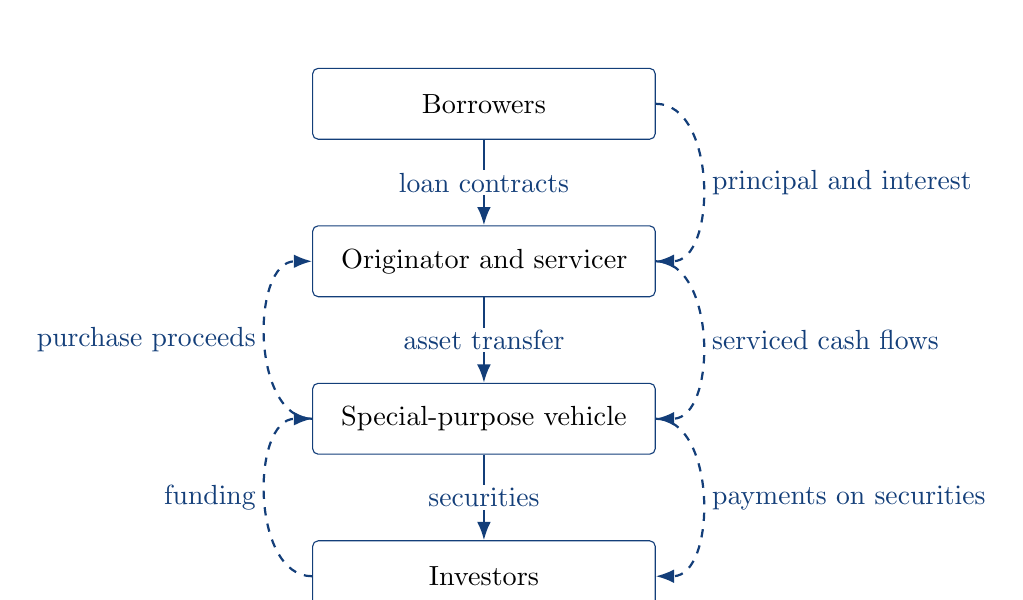
\begin{tikzpicture}[
  >=Latex,
  box/.style={
    draw=FinanceBlue,
    rounded corners=2pt,
    align=center,
    text width=4.0cm,
    minimum height=0.9cm,
    inner sep=5pt
  },
  flow/.style={
    -Latex,
    line width=0.8pt,
    FinanceBlue
  },
  mainlabel/.style={
  fill=white,
  inner xsep=3pt,
  inner ysep=1pt,
  text=FinanceBlue
},
  backflow/.style={
    -Latex,
    dashed,
    line width=0.8pt,
    FinanceBlue
  }
]

% Nodes
\node[box] (borrowers) at (0,0) {Borrowers};
\node[box] (originator) at (0,-2.0) {Originator and servicer};
\node[box] (spv) at (0,-4.0) {Special-purpose vehicle};
\node[box] (investors) at (0,-6.0) {Investors};

% Contractual / structural chain
\draw[flow]
  (borrowers) --
  node[midway,mainlabel]{loan contracts}
  (originator);

\draw[flow]
  (originator) --
  node[midway,mainlabel]{asset transfer}
  (spv);

\draw[flow]
  (spv) --
  node[midway,mainlabel]{securities}
  (investors);

% Funding and cash-flow chain
\draw[backflow]
  (investors.west)
  to[out=180,in=180]
  node[left]{funding}
  (spv.west);

\draw[backflow]
  (spv.west)
  to[out=180,in=180]
  node[left]{purchase proceeds}
  (originator.west);

\draw[backflow]
  (borrowers.east)
  to[out=0,in=0]
  node[right]{principal and interest}
  (originator.east);

\draw[backflow]
  (originator.east)
  to[out=0,in=0]
  node[right]{serviced cash flows}
  (spv.east);

\draw[backflow]
  (spv.east)
  to[out=0,in=0]
  node[right]{payments on securities}
  (investors.east);

\end{tikzpicture}

\caption{A simplified securitization chain}
\label{fig:ch20-securitization-chain}

\end{figure}



The diagram abstracts from trustees, custodians, arrangers, rating agencies, liquidity providers, hedge counterparties, and other participants. These institutions may affect the operation and risk of particular transactions, but the basic structure is captured by the transfer of assets, the issuance of securities, and the movement of cash flows through the vehicle.


\subsection{Asset Pooling and Cash-Flow Aggregation}

Once assets are transferred into the securitization structure, their cash flows are combined at the pool level. Mortgages, auto loans, consumer loans, leases, or receivables that were originally separate contractual claims can thus provide a common source of cash flow for the securities backed by the pool.

Suppose the pool contains \(n\) assets. Let \(CF_{i,t}\) denote the cash flow generated by asset \(i\) at date \(t\). Before servicing fees, transaction expenses, and other structural deductions, aggregate pool cash flow is

\begin{equation}
CF_t^{A}
=
\sum_{i=1}^{n} CF_{i,t}.
\label{eq:ch20-pool-cash-flow}
\end{equation}

Pooling can reduce the importance of individual borrower outcomes relative to the pool as a whole. A prepayment or delinquency on one loan may have only a limited effect on aggregate cash flow when exposures are sufficiently dispersed. The extent of diversification, however, depends on the dependence among the underlying assets.

Let \(L_i\) denote the loss on asset \(i\). Total pool loss is

\begin{equation}
L_A
=
\sum_{i=1}^{n} L_i.
\label{eq:ch20-pool-loss}
\end{equation}

Its variance is

\begin{equation}
\operatorname{Var}(L_A)
=
\sum_{i=1}^{n}\operatorname{Var}(L_i)
+
\sum_{i\neq j}\operatorname{Cov}(L_i,L_j).
\label{eq:ch20-pool-loss-variance}
\end{equation}

The covariance terms capture common variation across exposures. When borrower outcomes are only weakly related, individual shocks tend to have less influence on the performance of a large pool. When many borrowers are exposed to the same housing market, region, industry, interest-rate environment, or macroeconomic condition, losses may rise together. A large number of assets therefore need not imply strong diversification.

Evaluating pooled cash flows consequently requires information about both the individual assets and their distribution across the pool. Underwriting standards, borrower quality, collateral values, seasoning, geographic concentration, payment status, and recovery experience can affect both expected cash flows and the extent to which losses move together.

Realized pool cash flow also depends on servicing after origination. The servicer collects payments, manages delinquencies, processes modifications, and handles recoveries where relevant. Pool performance therefore reflects not only the characteristics of the assets at transfer but also the subsequent administration of the underlying contracts.

\subsection[Special-Purpose Vehicles and Bankruptcy Remoteness]{Special-Purpose Vehicles and Bankruptcy Remoteness}

Pooling creates a common source of cash flow, but the asset pool also needs a legal and contractual structure through which those cash flows can support securities. The special-purpose vehicle provides that structure. It acquires the transferred assets and issues claims whose payments depend primarily on the performance of the pool.

A central objective is to reduce the exposure of the securitized assets to the general insolvency risk of the originator. If the asset transfer is legally effective and the vehicle is structured with sufficient separation, creditors of the originator may have limited access to the transferred assets if the originator later enters insolvency. This feature is commonly described as bankruptcy remoteness.

The legal character of the transfer is therefore important. A transaction structured as a true sale seeks to transfer ownership of the assets to the SPV rather than leave the arrangement economically equivalent to secured borrowing. If a transfer were recharacterized as secured financing, the treatment of the assets in the originator's insolvency could differ.

Bankruptcy remoteness also depends on the structure of the vehicle itself. SPVs are generally limited in purpose, borrowing, asset substitution, and other activities. These restrictions can reduce the possibility that unrelated business risks or additional creditors enter the structure. Contractual provisions may also govern accounts, servicing arrangements, payment procedures, and events that alter the normal operation of the vehicle.

The originator may nevertheless remain connected to the structure as servicer, holder of a retained interest, provider of representations and warranties, or source of limited liquidity support. The degree of economic separation can therefore vary across transactions.

\begin{tcolorbox}[
  enhanced,
  breakable,
  colback=white,
  colframe=FinanceBlue,
  boxrule=0.7pt,
  sharp corners,
  borderline west={2.2pt}{0pt}{FinanceBlue},
  title=\textbf{Financial Perspective: Bankruptcy Remoteness Is Legal Separation, Not Credit Protection by Itself},
  coltitle=white,
  colbacktitle=FinanceBlue,
  fonttitle=\bfseries,
  before skip=1.2em,
  after skip=1.2em
]

Bankruptcy remoteness can reduce investors' exposure to the originator's general insolvency by separating the transferred assets from the originator. It does not, by itself, improve the payment capacity of the underlying borrowers. Credit quality and legal separation are distinct features of the structure.

\end{tcolorbox}


\subsection{Asset-Backed and Mortgage-Backed Securities}

The assets held within a securitization structure can differ substantially in their contractual and economic characteristics. In market usage, asset-backed securities (ABS) generally refer to securities backed by non-mortgage assets such as auto loans, consumer loans, leases, and receivables, while mortgage-backed securities (MBS) are supported by residential or commercial mortgage cash flows.

These underlying assets differ in maturity, amortization, collateral, borrower behavior, and sensitivity to economic conditions. Such differences affect both the amount and timing of cash flows available to the securities issued against the pool.Examples of major securitized asset classes, together with their typical cash-flow characteristics and principal risks, are summarized in Table~\ref.{tab:ch20-securitized-assets}.

\begin{table}[H]

\centering

\caption{Selected securitized asset classes and cash-flow characteristics}

\label{tab:ch20-securitized-assets}

\begin{tabularx}{\textwidth}{@{}p{3.4cm}YY@{}}

\toprule

\textbf{Underlying assets} &
\textbf{Typical cash-flow characteristics} &
\textbf{Principal risks} \\

\midrule

Auto loans &
Scheduled amortization of principal and interest &
Default, vehicle recovery values, prepayment \\

Consumer loans &
Installment payments over contractual maturities &
Default, seasoning, borrower income conditions \\

Credit-card receivables &
Revolving balances, principal collections, and finance charges &
Payment rates, charge-offs, changing balances \\

Residential mortgages &
Long-dated amortizing principal and interest payments &
Default, collateral values, prepayment, interest rates \\

Commercial mortgages &
Property-related debt service, often with relatively large individual exposures &
Property income, refinancing, concentration, maturity risk \\

\bottomrule

\end{tabularx}

\end{table}

The securitization structure determines how these asset-level cash flows are transmitted to investors. Some securities pass principal and interest collections through after specified fees and adjustments. Others divide the same pool cash flows among classes with different payment priorities, maturities, or exposure to particular risks.

Mortgage prepayment provides an important example of this transmission. When borrowers refinance or repay mortgages early, principal reaches MBS investors sooner than originally scheduled, which can shorten the expected life of the securities and increase reinvestment exposure. When prepayments slow, principal may remain outstanding longer than expected. The mortgages need not default for the timing and value of investor cash flows to change.

ABS and MBS therefore differ not only in the assets that support them, but also in how the contractual and behavioral features of those assets are transmitted through the securitization structure.


\section[Tranching, Credit Enhancement, and Risk Allocation]{Tranching, Credit Enhancement, and Risk Allocation}

Once cash flows from the asset pool enter the securitization structure, their allocation across securities becomes a contractual design problem. Tranching establishes differences in payment priority and loss absorption, while credit enhancement provides additional protection to particular tranches.

\subsection{Seniority, Payment Priority, and Loss Allocation}

Within a tranched structure, seniority is implemented through contractual rules governing the distribution of available cash and the allocation of losses. A payment waterfall specifies the order in which available cash is distributed across security classes.

Let \(C_t\) denote cash available for distribution at date \(t\) after permitted expenses. Suppose the structure contains scheduled senior and mezzanine payments, \(D_{S,t}\) and \(D_{M,t}\), together with a junior residual claim.

The senior tranche receives

\begin{equation}
P_{S,t}
=
\min\{D_{S,t},C_t\}.
\label{eq:ch20-senior-waterfall}
\end{equation}

The mezzanine tranche receives

\begin{equation}
P_{M,t}
=
\min\left\{
D_{M,t},
\max\{C_t-P_{S,t},0\}
\right\}.
\label{eq:ch20-mezz-waterfall}
\end{equation}

The junior tranche receives the residual cash flow,

\begin{equation}
P_{J,t}
=
\max\{
C_t-P_{S,t}-P_{M,t},
0
\}.
\label{eq:ch20-junior-waterfall}
\end{equation}

These expressions describe a simplified sequential waterfall. Actual structures may maintain separate interest and principal waterfalls, apply coverage tests, trap excess cash, redirect principal, or alter payment priorities after specified trigger events.

\begin{example}{A Simple Payment Waterfall}{simple-structured-waterfall}

A securitization has RMB~70 million of senior payments due, RMB~20 million of mezzanine payments due, and a junior residual interest.

If RMB~100 million is available for distribution, the senior tranche receives 70, the mezzanine tranche receives 20, and the junior tranche receives the remaining 10.

If only RMB~82 million is available, the senior tranche receives 70, the mezzanine tranche receives 12, and the junior tranche receives nothing.

A reduction in available cash does not affect all tranches proportionally. Payment priority causes the initial shortfall to fall on more subordinated claims.

\end{example}

Payment priority governs the distribution of available cash. Loss allocation determines how deterioration in the asset pool reduces the value of the different tranches. In a simple subordinated structure, losses are absorbed in the reverse order of payment priority: junior claims are affected first, followed by mezzanine and then senior claims.

Let the initial tranche notionals be \(N_J\), \(N_M\), and \(N_S\), and let \(L\) denote cumulative loss allocated to the tranches. Junior loss is

\begin{equation}
L_J
=
\min\{L,N_J\}.
\label{eq:ch20-junior-loss}
\end{equation}

Mezzanine loss is

\begin{equation}
L_M
=
\min\left\{
\max\{L-N_J,0\},
N_M
\right\},
\label{eq:ch20-mezz-loss}
\end{equation}
and senior loss is

\begin{equation}
L_S
=
\min\left\{
\max\{L-N_J-N_M,0\},
N_S
\right\}.
\label{eq:ch20-senior-loss}
\end{equation}

The waterfall does not alter the loss generated by the underlying asset pool. It changes how that loss is distributed across tranches and the level of cumulative loss at which each tranche begins to be affected.

\subsection{Internal Credit Enhancement}

The same priority structure that allocates losses across tranches can also provide credit enhancement. Internal credit enhancement protects particular tranches by placing subordinated claims or other transaction resources ahead of them in absorbing losses or cash-flow shortfalls.

Subordination provides protection through the ordering of tranche losses. Junior and mezzanine claims absorb losses before more senior claims. If the amount ranking below a senior tranche is \(N_J+N_M\), the amount of subordinated protection is

\begin{equation}
SR
=
\frac{N_J+N_M}{N_A},
\label{eq:ch20-subordination-ratio}
\end{equation}
where \(N_A\) is the relevant asset-pool balance. A larger subordinated layer generally allows the senior tranche to withstand greater pool losses before its principal is affected, subject to the contractual allocation rules.

Overcollateralization provides protection by maintaining an asset balance larger than the principal amount of securities issued against it. If asset principal is \(N_A\) and issued securities total \(N_S\),

\begin{equation}
OC
=
N_A-N_S,
\label{eq:ch20-overcollateralization}
\end{equation}
with an overcollateralization ratio

\begin{equation}
OCR
=
\frac{N_A-N_S}{N_A}.
\label{eq:ch20-overcollateralization-ratio}
\end{equation}

The excess asset balance provides a cushion against deterioration in pool value or collections before an equivalent principal shortfall reaches the issued securities.

A reserve account holds cash or eligible investments that can be used to cover specified shortfalls. It may be funded at closing or accumulated from transaction cash flows over time. Its protective value depends on both its size and the contractual conditions governing its use.

Excess spread arises when interest and fee income from the asset pool exceeds servicing expenses, security payments, and other permitted costs. When retained within the structure, this excess cash flow can absorb certain losses or replenish other forms of enhancement before principal claims are affected. Its availability can vary with defaults, prepayments, asset yields, and other changes in pool performance. Excess spread is one of several forms of internal credit enhancement. The main mechanisms, their sources of protection, and their limitations are summarized in Table~\ref.{tab:ch20-internal-enhancement}.

\begin{table}[H]

\centering

\caption{Selected forms of internal credit enhancement}

\label{tab:ch20-internal-enhancement}

\begin{tabularx}{\textwidth}{@{}p{3.5cm}YY@{}}

\toprule
\textbf{Mechanism} &
\textbf{Source of protection} &
\textbf{Main limitation} \\
\midrule

Subordination &
Junior claims absorb losses before senior claims &
Protection can be exhausted as cumulative pool losses increase \\

Overcollateralization &
Asset balance exceeds issued security balance &
Deterioration in the asset pool can erode the excess collateral \\

Reserve account &
Cash or eligible assets cover specified shortfalls &
Available resources are finite and subject to contractual use \\

Excess spread &
Asset income exceeds required payments and expenses &
Available spread can decline as pool performance changes \\

\bottomrule

\end{tabularx}

\end{table}

These mechanisms alter the resources and priorities through which losses and shortfalls reach different tranches. They can strengthen the protection of selected claims without changing the payment capacity of the underlying borrowers.

\subsection{External Credit Enhancement}

Internal credit enhancement draws on resources within the securitization structure. External credit enhancement instead adds a contractual commitment from a third party, such as a guarantor, insurer, or bank providing a letter of credit. The third party agrees to cover specified shortfalls subject to the terms and limits of the arrangement.

Suppose a tranche experiences a covered shortfall \(X_t\), and the available guarantee amount is \(G_t\). The support payment can be represented as

\begin{equation}
H_t
=
\min\{X_t,G_t\}.
\label{eq:ch20-guarantee-payment}
\end{equation}

For the covered amount, the investor acquires a claim on the protection provider rather than bearing the asset-pool shortfall directly. The value of this protection therefore depends on both the contractual coverage and the provider's capacity to perform. If the provider becomes weaker under the same conditions that impair the asset pool, the effective protection may be less than the contractual limit suggests.

Liquidity support serves a related but different purpose. A liquidity facility can bridge temporary timing mismatches when expected cash has not yet been received, whereas credit enhancement provides protection against specified economic losses. A facility may contain elements of both, but the two functions are conceptually distinct.

\begin{tcolorbox}[
  enhanced,
  breakable,
  colback=white,
  colframe=FinanceBlue,
  boxrule=0.7pt,
  sharp corners,
  borderline west={2.2pt}{0pt}{FinanceBlue},
  title=\textbf{Financial Perspective: Credit Enhancement Redistributes Loss-Bearing Capacity},
  coltitle=white,
  colbacktitle=FinanceBlue,
  fonttitle=\bfseries,
  before skip=1.2em,
  after skip=1.2em
]

Credit enhancement protects selected claims by placing other resources ahead of them in absorbing losses. These resources may come from subordinated tranches, excess collateral, reserves, retained cash flows, or external counterparties. The underlying asset-pool loss is not eliminated; the structure changes where and when that loss reaches investors.

\end{tcolorbox}

\subsection{Risk Allocation across Tranches and Investors}

Once payment priorities and credit-enhancement arrangements are specified, each tranche has a distinct exposure to losses from the same asset pool. Attachment and detachment points provide a compact way to describe these differences and connect the structure of the transaction to the risks borne by investors.

Consider a structure in which the junior tranche occupies the first 10\% of pool principal, the mezzanine tranche the next 15\%, and the senior tranche the remaining 75\%. The junior tranche attaches at zero and detaches at 10\%. The mezzanine tranche attaches at 10\% and detaches at 25\%, while the senior tranche begins to absorb principal losses only after cumulative pool losses exceed 25\% under this simplified structure.

For a tranche with attachment point \(a\) and detachment point \(d\), expressed as fractions of the original pool balance, the fraction of tranche principal lost when the cumulative pool loss rate is \(\ell\) can be written as

\begin{equation}
TL(\ell)
=
\frac{
\min\{\max\{\ell-a,0\},d-a\}
}{
d-a
}.
\label{eq:ch20-tranche-loss-function}
\end{equation}

The loss profile is nonlinear. Pool losses below the attachment point leave the tranche principal unaffected. Losses between the attachment and detachment points are transmitted to the tranche, while losses beyond the detachment point imply full principal impairment. A given change in pool loss can therefore have very different effects across the capital structure.

\begin{example}{Attachment, Detachment, and Tranche Loss}{tranche-loss-example}

Consider a RMB~100 million asset pool divided into three tranches:

\[
\text{Junior}=10,\qquad
\text{Mezzanine}=15,\qquad
\text{Senior}=75.
\]

The mezzanine tranche attaches at 10\% and detaches at 25\% of the pool balance. Suppose cumulative pool loss reaches 18\%. The first 10\% is absorbed by the junior tranche, leaving 8\% of pool principal to be absorbed by the mezzanine tranche.

Using the tranche-loss function,

\[
TL(0.18)
=
\frac{0.18-0.10}{0.25-0.10}
=
\frac{0.08}{0.15}
\approx 53.3\%.
\]

The pool has lost 18\% of its original principal, but the mezzanine tranche has lost approximately 53.3\% of its own principal. The attachment and detachment points therefore translate a pool-level loss into a much larger loss rate for a particular tranche.

\end{example}

These differences create claims suited to investors with different objectives and constraints. Investors willing to bear first-loss exposure may require a higher expected return, while investors placing greater weight on protection against moderate losses may prefer more senior claims. Liability structure, liquidity needs, regulatory treatment, investment mandates, and assessments of tail risk can also influence tranche demand.

Seniority reduces exposure to initial pool losses but does not eliminate sensitivity to severe common shocks. When losses across underlying assets become more strongly dependent, subordinated protection may be exhausted more rapidly. The risk of a senior tranche therefore depends not only on expected pool loss but also on the distribution and dependence of losses in adverse states.

Tranching thus maps a common pool-loss distribution into different loss profiles across investors. The claims may differ substantially in expected loss and tail exposure even though they are supported by the same underlying assets.

\section{Financial Engineering, Complexity, and Fragility}

Tranching redistributes losses from a common asset pool across investors. Financial engineering can extend this process through additional contractual layers, funding arrangements, and forms of risk transfer. As these elements interact, the risk of a security may depend not only on the underlying assets but also on payment rules, model assumptions, counterparties, and liquidity conditions.

Complexity matters when these dependencies make exposures harder to trace, value, or monitor. It does not necessarily imply fragility, but fragility can increase when losses, funding pressures, or valuation changes are amplified through interconnected structures or when protection weakens under common shocks.

\subsection[CDOs, Re-Securitization, and Structural Complexity]{CDOs, Re-Securitization, and Structural Complexity}

The interaction among multiple contractual layers becomes especially visible when debt securities themselves enter a new structured pool. A collateralized debt obligation (CDO) pools debt instruments and issues tranches against the resulting portfolio. The collateral may include corporate loans, bonds, or structured securities. A collateralized loan obligation (CLO), for example, is backed primarily by a portfolio of corporate loans.

When structured securities themselves become collateral for another transaction, re-securitization adds a further layer between the original assets and the final investors. Tranches from several mortgage-backed or asset-backed structures can, for example, be combined to support a new set of securities. A simplified chain is
summarized in Figure~\ref{fig:ch20-resecuritization-chain}.
\begin{figure}[htbp]
\centering

\begin{tikzpicture}[
  >=Latex,
  box/.style={
    draw=FinanceBlue,
    rounded corners=2pt,
    align=center,
    text width=2.3cm,
    minimum height=1.0cm,
    inner sep=5pt
  },
  flow/.style={
    -Latex,
    line width=0.8pt,
    FinanceBlue
  }
]

\node[box] (loans) at (0,0) {Underlying\\loans};
\node[box] (abs) at (3.2,0) {ABS/MBS\\tranches};
\node[box] (pool) at (6.4,0) {Resecuritized\\pool};
\node[box] (new) at (9.6,0) {New\\tranches};

\draw[flow] (loans) -- (abs);
\draw[flow] (abs) -- (pool);
\draw[flow] (pool) -- (new);

\end{tikzpicture}

\caption{A stylized re-securitization chain}
\label{fig:ch20-resecuritization-chain}

\end{figure}

The additional layer changes the information required to evaluate the final securities. Their performance may depend not only on the underlying loans, but also on the tranche positions of the collateral securities and the contractual rules of the structures in which those securities were issued.

Dependence is particularly important. Securities drawn from different transactions may appear diversified while their underlying pools remain exposed to common property markets, underwriting practices, refinancing conditions, or macroeconomic shocks. Losses across the collateral securities can therefore become more closely related in adverse states than the number of separate transactions might suggest.

Evaluation may consequently require information at several levels: the final tranche, the securities held as collateral, the pools supporting those securities, and the dependence among the underlying exposures. As the number of layers increases, valuation can become more sensitive to data quality and assumptions about default, recovery, and loss dependence.

Structured exposure can also be created synthetically through credit derivatives rather than through direct ownership of all referenced debt instruments. When synthetic exposure is combined with tranching, the investor's payoff depends on both the referenced credit events and the contractual terms governing their transmission through the structure.

Structural complexity therefore arises not simply from the number of securities involved, but from the number and interaction of contractual links through which underlying losses reach the final investor.

\subsection{Originate-to-Distribute Incentives and Moral Hazard}

The same separation that can make risk more difficult to trace can also affect incentives. When origination, distribution, servicing, and ultimate risk bearing are divided among different parties, those with the best information about a loan may bear only part of its subsequent performance.

Consider an originator that earns revenue when loans are originated and transferred into a securitization. If it retains only limited exposure to subsequent credit losses, the private return to costly screening may be lower than when the loan remains largely on its balance sheet. When screening effort is difficult for investors to observe, this separation can create a moral-hazard problem.

The strength of this incentive effect varies across transactions. Risk retention, representations and warranties, repurchase obligations, reputation, repeated access to capital markets, and investor due diligence can reconnect origination decisions with subsequent loan performance.

These mechanisms operate through different channels. A retained junior interest exposes the originator directly to early pool losses. Representations and warranties can require the originator to repurchase or compensate for loans that fail to satisfy specified contractual standards. Their effectiveness depends on the exposure retained, the information available to investors, and the enforceability of the relevant obligations.

Incentive differences can also arise during servicing. Decisions about collection, modification, foreclosure, and recovery affect the timing and amount of cash flows reaching investors. The servicer may not bear the same economic exposure as security holders, while investors in different tranches may prefer different responses to borrower distress. Incentive conflicts can arise at different stages of the originate-to-distribute process. Table~\ref{tab:ch20-otd-incentives} summarizes the potential incentive problems faced by major participants and the mechanisms that may help mitigate them.

\begin{table}[H]

\centering

\caption{Selected incentive links in an originate-to-distribute structure}

\label{tab:ch20-otd-incentives}

\begin{tabularx}{\textwidth}{@{}p{3.4cm}YY@{}}

\toprule
\textbf{Participant} &
\textbf{Potential incentive problem} &
\textbf{Possible mitigating mechanism} \\
\midrule

Originator &
Origination revenue may be realized before long-term loan performance is known &
Risk retention, representations and warranties, repurchase obligations \\

Arranger &
Structuring and distribution revenue may differ from subsequent investor loss exposure &
Reputation, disclosure, due diligence, retained exposure \\

Servicer &
Servicing decisions can affect investors and tranches differently &
Servicing standards, performance triggers, replacement provisions \\

Investor &
Limited information acquisition can increase reliance on external assessments &
Due diligence, disclosure, position limits, transparency requirements \\

\bottomrule

\end{tabularx}

\end{table}

The incentive problem therefore depends on how closely information production, decision making, and loss bearing remain connected within the securitization structure.


\subsection[Information Opacity, Model Risk, and Rating Failures]{Information Opacity, Model Risk, and Rating Failures}

The separation of origination, servicing, structuring, and risk bearing also disperses information across different parties. Investors may observe some features of the underlying assets while having less direct access to underwriting quality, servicing practices, contractual details, or the interactions among these elements. Information opacity arises when relevant information is difficult to combine, verify, or trace through the structure.

Models help translate asset characteristics and contractual rules into expected losses, tranche-loss distributions, spreads, or values. Their results can depend materially on assumptions about default and prepayment dependence, recovery rates, common economic factors, attachment and detachment points, and contractual triggers. These assumptions become especially important when security payoffs respond nonlinearly to changes in collateral performance.

Model risk arises when the model structure, parameters, or data do not adequately represent these relationships. A tranche that appears well protected under one set of assumptions may become more exposed when dependence, recovery, or other conditions change.

Credit ratings provide a further form of information compression by mapping a complex security into an ordinal category. For a structured tranche, the assessment may reflect not only the credit quality of the underlying assets but also diversification, loss dependence, structural protection, and the tranche's position in the capital structure.

Rating performance can deteriorate when models or data fail to capture relevant risks, underwriting standards change, conflicts of interest affect the assessment process, or investors place excessive weight on the rating itself. A rating can therefore reduce information-processing costs without revealing every dimension of the security's risk.

\begin{tcolorbox}[
  enhanced,
  breakable,
  colback=white,
  colframe=FinanceBlue,
  boxrule=0.7pt,
  sharp corners,
  borderline west={2.2pt}{0pt}{FinanceBlue},
  title=\textbf{Financial Perspective: A Rating Does Not Reveal the Shape of Tail Risk},
  coltitle=white,
  colbacktitle=FinanceBlue,
  fonttitle=\bfseries,
  before skip=1.2em,
  after skip=1.2em
]

Two securities can carry similar ratings while deriving their risk from different economic structures. A corporate bond may depend primarily on the repayment capacity of one issuer, while a senior structured tranche may depend on both subordinated protection and the joint behavior of losses across an asset pool. Similar assessments of expected loss can therefore coexist with different sensitivities to adverse states.

\end{tcolorbox}

\subsection[Structured Finance Lessons from the Global Financial Crisis]{Structured Finance Lessons from the Global Financial Crisis}

Information opacity, model dependence, and reliance on ratings became especially consequential during the global financial crisis, when weaknesses in mortgage origination, securitization structures, and market liquidity interacted.

In the years preceding the crisis, U.S. mortgage lending expanded, including lending to borrowers with weaker credit characteristics. Many mortgages entered private-label mortgage-backed securities, while some structured claims were subsequently used as collateral for additional securitizations. These layers increased the information required to trace the final securities back to the performance of the underlying loans.

As mortgage performance deteriorated and housing prices declined, losses became more closely related across pools exposed to similar economic conditions. Subordinated tranches absorbed initial losses, but larger and more widespread deterioration reduced the protection available to mezzanine and senior claims. At the same time, uncertainty about valuation made some structured securities more difficult to trade or finance.

The episode illustrates how several mechanisms can reinforce one another under stress. Weak underwriting can worsen the losses entering an asset pool, common exposures can limit diversification, and structural layering can make those risks harder to identify and value. Tranching determines where losses are absorbed, while funding and market liquidity influence how valuation changes affect investors and intermediaries. The main structured-finance mechanisms illustrated by the crisis, their economic functions, and the risks they revealed under stress are summarized in Table~\ref{tab:ch20-crisis-lessons}.

\begin{table}[H]

\centering

\caption{Structured-finance mechanisms and lessons from the global financial crisis}

\label{tab:ch20-crisis-lessons}

\begin{tabularx}{\textwidth}{@{}p{3.5cm}YY@{}}

\toprule
\textbf{Mechanism} &
\textbf{Economic function} &
\textbf{Risk revealed under stress} \\
\midrule

Pooling &
Combines exposures and can reduce borrower-specific risk &
Common exposures can generate correlated losses \\

Tranching &
Allocates losses across claims with different priorities &
Severe pool losses can exhaust subordinated protection \\

Originate-to-distribute &
Separates origination, funding, and risk bearing &
Limited retained exposure can weaken screening incentives \\

Ratings and models &
Compress complex information into tractable risk assessments &
Common assumptions can produce similar valuation errors \\

Re-securitization &
Creates additional layers of risk allocation &
Underlying exposures can become more difficult to trace and evaluate \\

\bottomrule

\end{tabularx}

\end{table}

The broader lesson is that the performance of structured claims depends on the interaction among asset quality, dependence across exposures, contractual protection, incentives, valuation, and market liquidity.


%========================================================
% Summary
%========================================================

\TailModule{summary}{Summary}

Structured finance reorganizes cash flows from existing financial assets into securities with different contractual characteristics. In a cash securitization, loans or receivables are transferred to a special-purpose vehicle (SPV), pooled, and financed through securities issued to investors. Pooling can reduce the influence of borrower-specific outcomes, although exposure to common economic factors may remain substantial.

The SPV provides a separate legal and contractual structure for the asset pool and can support bankruptcy remoteness when the transfer and organizational arrangements are legally effective. The characteristics of the underlying assets---including maturity, amortization, default, collateral, and prepayment behavior---shape the cash flows available to ABS and MBS investors.

Tranching allocates those cash flows and losses across claims with different priorities. Senior tranches receive greater protection from initial losses, while subordinated tranches absorb losses earlier. Subordination, overcollateralization, reserve accounts, excess spread, and external support can further protect selected claims by providing additional loss-bearing capacity. These mechanisms redistribute exposure to asset-pool losses rather than removing the losses themselves.

Additional layers of structuring can broaden the ways in which risk is allocated, while increasing informational and modeling demands. Re-securitization can make underlying exposures and dependence more difficult to trace, and originate-to-distribute arrangements can weaken screening incentives when origination becomes insufficiently connected to subsequent loss bearing. The global financial crisis illustrated how underwriting quality, correlated asset losses, model dependence, reliance on ratings, and market liquidity can interact within structured-finance chains.


%========================================================
% Mind Map
%========================================================

\begin{figure}[H]
\centering
\begin{tikzpicture}[
  >=Latex,
  main/.style={
    draw=FinanceBlue,
    fill=FinanceBlue!7,
    rounded corners=2pt,
    align=center,
    text width=4.2cm,
    minimum height=1.0cm,
    inner sep=5pt
  },
  sub/.style={
    draw=FinanceBlue,
    rounded corners=2pt,
    align=center,
    text width=4.0cm,
    minimum height=0.9cm,
    inner sep=5pt
  },
  arrow/.style={-Latex,line width=0.8pt,FinanceBlue},
  subarrow/.style={-Latex,dashed,line width=0.8pt,FinanceBlue}
]

% Main vertical chain
\node[main] (assets) at (0,0) {Underlying assets\\and borrower cash flows};
\node[main] (pool) at (0,-2.2) {SPV, pooling, and\\cash-flow aggregation};
\node[main] (structure) at (0,-4.4) {Waterfall and\\credit enhancement};
\node[main] (investors) at (0,-6.6) {Tranches with different\\risk exposures};

\draw[arrow] (assets) -- (pool);
\draw[arrow] (pool) -- (structure);
\draw[arrow] (structure) -- (investors);

% Side analytical dimensions
\node[sub] (info) at (6.0,-2.2) {\textbf{Information}\\underwriting, pool composition, servicing};
\node[sub] (contract) at (6.0,-4.4) {\textbf{Contracts}\\priority, triggers, guarantees};
\node[sub] (value) at (6.0,-6.6) {\textbf{Valuation}\\dependence, prepayment, tail risk};

\draw[subarrow] (pool.east) -- (info.west);
\draw[subarrow] (structure.east) -- (contract.west);
\draw[subarrow] (investors.east) -- (value.west);

\end{tikzpicture}
\caption{Structured finance through information, contracts, and valuation}
\label{fig:ch20-mind-map}
\end{figure}


%========================================================
% Key Terms
%========================================================

\TailModule{keyterms}{Key Terms}

Structured finance; securitization; originate-to-distribute;
asset pool; servicer; special-purpose vehicle (SPV);
bankruptcy remoteness; true sale; asset-backed security (ABS);
mortgage-backed security (MBS); prepayment risk; tranche;
payment waterfall; loss waterfall; attachment point; detachment point;
subordination; overcollateralization; reserve account;
collateralized debt obligation (CDO); re-securitization;
risk retention; model risk; common-factor risk.


%========================================================
% Financial AI Lab
%========================================================

\TailModule{aiprompt}{Financial AI Lab}

\textbf{Lab: Audit a Securitization Waterfall and Risk Narrative}

Ask an AI system to analyze a securitization backed by a RMB~100 million loan pool. The structure contains a RMB~70 million senior tranche, a RMB~20 million mezzanine tranche, and a RMB~10 million junior tranche.

Audit the analysis in five stages.

\begin{enumerate}

\item \textbf{Map the transaction before analyzing the securities.}

Identify the borrower pool, originator, SPV, servicer, and investors. Verify that the AI system distinguishes the underlying assets from the securities issued against them and traces the direction of asset transfers, funding, and cash flows.

\item \textbf{Recalculate the loss waterfall.}

Calculate the principal loss allocated to each tranche when cumulative pool losses equal RMB~5 million, RMB~15 million, RMB~25 million, and RMB~35 million. Determine the attachment and detachment points of each tranche and check whether the AI system applies the loss priority correctly.

\item \textbf{Identify the source of credit enhancement.}

Determine which protection is actually present in the stated structure. Distinguish subordination from overcollateralization, reserve accounts, excess spread, and external guarantees. Do not infer forms of enhancement that are not supported by the transaction information, and identify which party or resource provides the relevant loss-bearing capacity.

\item \textbf{Stress the dependence assumption.}

Compare a pool dominated by borrower-specific shocks with one exposed to a common housing, industry, or macroeconomic shock. Explain how stronger dependence among borrowers can change the tail-loss distribution even when the number of loans is unchanged.

\item \textbf{Audit the rating or valuation narrative.}

If the AI system treats a high rating as sufficient evidence of low risk, identify the assumptions supporting that assessment. Examine loss dependence, recovery, attachment and detachment points, structural protection, and other common-factor exposures that could affect the tranche under adverse conditions.

\end{enumerate}


%========================================================
% Discussion Questions
%========================================================

\TailModule{questions}{Discussion Questions}

\begin{enumerate}

\item How does cash securitization differ from synthetic credit-risk transfer?

\item Why can pooling reduce borrower-specific risk without eliminating exposure to common economic shocks?

\item What role does an SPV play in securitization, and why is bankruptcy remoteness different from protection against borrower default?

\item How do payment priority and subordination create different risk exposures across tranches without changing total asset-pool loss?

\item How can originate-to-distribute improve funding flexibility while also affecting screening and monitoring incentives?

\item Why can re-securitization, model dependence, and reliance on ratings make the risk of structured securities more difficult to evaluate, particularly in adverse states?

\end{enumerate}


%========================================================
% Applied Problems
%========================================================

\TailModule{appprobs}{Applied Problems}

\begin{enumerate}

\item \textbf{Pool cash-flow aggregation.}

A securitization pool contains three loans. At date \(t\), Loan A pays RMB~2.0 million, Loan B pays RMB~1.5 million, and Loan C pays RMB~1.0 million.

\begin{enumerate}

\item Calculate total pool cash flow using Equation~\eqref{eq:ch20-pool-cash-flow}.

\item Suppose Loan B misses its entire payment. Calculate the new pool cash flow.

\item Explain how the effect of one missed payment would change if the pool contained hundreds of similarly sized loans with largely independent borrower-specific risks.

\item Explain why the diversification effect can be weaker when many loans share the same regional, industry, or macroeconomic exposure.

\end{enumerate}


\item \textbf{SPV financing and retained risk.}

An SPV acquires a RMB~500 million loan pool. It finances the acquisition with RMB~470 million of securities sold to outside investors and a RMB~30 million junior interest retained by the originator.

\begin{enumerate}

\item Reconcile the financing of the RMB~500 million asset purchase.

\item Distinguish the funding provided by outside investors from the exposure retained by the originator.

\item Explain how retention of the junior interest affects the allocation of initial pool losses.

\item Explain why transferring the loans to the SPV does not improve the borrowers' repayment capacity.

\end{enumerate}


\item \textbf{Payment waterfall.}

A securitization has RMB~60 million of senior payments due and RMB~25 million of mezzanine payments due in the current period. The junior tranche receives residual cash flow.

\begin{enumerate}

\item Allocate RMB~100 million of available cash across the three classes.

\item Repeat the allocation when available cash equals RMB~72 million.

\item Repeat the allocation when available cash equals RMB~50 million.

\item Explain how payment priority determines the distribution of a cash-flow shortfall.

\end{enumerate}


\item \textbf{Loss waterfall and attachment points.}

A RMB~200 million asset pool supports a RMB~20 million junior tranche, a RMB~40 million mezzanine tranche, and a RMB~140 million senior tranche.

\begin{enumerate}

\item Calculate the attachment and detachment points of the mezzanine tranche as percentages of the original pool balance.

\item Allocate losses across the tranches when cumulative pool loss is RMB~15 million.

\item Repeat the calculation for cumulative losses of RMB~45 million and RMB~80 million.

\item Explain why the senior tranche can have relatively low expected loss while remaining exposed to severe common shocks.

\end{enumerate}


\item \textbf{Internal and external credit enhancement.}

An asset pool has principal of RMB~320 million, while securities issued against the pool total RMB~300 million. The structure also contains a RMB~6 million reserve account. A third-party guarantor covers eligible senior-tranche shortfalls up to RMB~25 million.

\begin{enumerate}

\item Calculate the amount and ratio of overcollateralization.

\item Calculate the combined nominal amount of overcollateralization and the reserve account before considering the detailed waterfall.

\item Calculate the guarantee payment when an eligible shortfall is RMB~12 million and when it is RMB~40 million.

\item Distinguish the sources of protection provided by overcollateralization, the reserve account, and the guarantee.

\item Explain why these amounts cannot necessarily be added to obtain a single measure of realized protection.

\end{enumerate}


\item \textbf{Originate-to-distribute incentives.}

A mortgage originator earns much of its revenue when a loan is originated and transferred into a securitization, while retaining only limited exposure to subsequent credit losses.

\begin{enumerate}
\item Explain how this arrangement can affect screening incentives when screening effort is difficult for investors to observe.

\item Explain how representations and warranties can reconnect the originator to subsequent loan performance.

\item Explain how retention of a junior interest can affect the originator's incentives.

\item Identify one potential cost of requiring the originator to retain a large share of credit risk.

\end{enumerate}


\item \textbf{Re-securitization and common exposure.}

A CDO holds mezzanine tranches from 30 mortgage securitizations. Each underlying securitization contains loans from many borrowers.

\begin{enumerate}

\item Explain why the CDO may appear diversified when viewed only by the number of collateral securities.

\item Identify three common factors that could cause losses across the underlying securitizations to rise together.

\item Explain why dependence assumptions are particularly important for the risk of the senior CDO tranche.

\item Describe the information an investor would need to trace the final security back through the collateral securities to the underlying asset pools.

\end{enumerate}

\end{enumerate}


%========================================================
% Case Analysis
%========================================================

\TailModule{caseanalysis}{Case Analysis}

\CaseLabel{Historical Case Based on Public Information}

\textbf{Private-Label Mortgage Securitization before the Global Financial Crisis}

Use an authoritative source such as the Financial Crisis Inquiry Commission, a central-bank publication, or a well-documented academic study to examine the U.S. private-label mortgage securitization chain in the years preceding the global financial crisis.

Organize the analysis around the structure of securitization rather than around a chronological narrative alone.

\begin{enumerate}

\item \textbf{Origination.}

Examine how mortgage underwriting standards and borrower characteristics affected the quality and risk distribution of the loans entering securitization.

\item \textbf{Pooling and structuring.}

Explain how mortgages were pooled and divided into securities with different payment priorities and loss exposures. Identify the role of subordination and other forms of credit enhancement.

\item \textbf{Distribution and information.}

Identify the main participants between mortgage origination and the final investor. Explain how information could become more dispersed, difficult to verify, or difficult to trace as the intermediation chain lengthened.

\item \textbf{Ratings and models.}

Examine the assumptions underlying the assessment of highly rated tranches. Consider house-price dynamics, default dependence, recovery rates, common-factor exposure, and structural protection rather than treating the rating itself as a complete measure of risk.

\item \textbf{Re-securitization.}

Explain how structured securities could themselves become collateral for CDOs or other re-securitized products, creating an additional layer of pooling, tranching, and dependence.

\item \textbf{Loss realization.}

Trace how deterioration in mortgage performance was transmitted through junior, mezzanine, and senior claims as subordinated protection was absorbed.

\item \textbf{Boundary with systemic amplification.}

Distinguish risks arising within the structured products from those amplified through leverage, funding pressure, market illiquidity, fire sales, and connections among financial institutions.

\end{enumerate}


%========================================================
% Further Reading
%========================================================

\TailModule{furtherread}{Further Reading}

\begin{itemize}

\item Ashcraft, Adam B., and Til Schuermann (2008),
``Understanding the Securitization of Subprime Mortgage Credit,''
\emph{Foundations and Trends in Finance}, 2(3), 191--309.

\item Coval, Joshua, Jakub Jurek, and Erik Stafford (2009),
``The Economics of Structured Finance,''
\emph{Journal of Economic Perspectives}, 23(1), 3--25.

\item Keys, Benjamin J., Tanmoy Mukherjee, Amit Seru, and Vikrant Vig (2010),
``Did Securitization Lead to Lax Screening? Evidence from Subprime Loans,''
\emph{The Quarterly Journal of Economics}, 125(1), 307--362.

\item Demyanyk, Yuliya, and Otto Van Hemert (2011),
``Understanding the Subprime Mortgage Crisis,''
\emph{The Review of Financial Studies}, 24(6), 1848--1880.

\item Gorton, Gary, and Andrew Metrick (2012),
``Securitized Banking and the Run on Repo,''
\emph{Journal of Financial Economics}, 104(3), 425--451.

\end{itemize}


\ChapterTail{summary,keyterms,aiprompt,questions,appprobs,caseanalysis,furtherread}


\part{Financial Stability, Policy, and Innovation}
\chapter{Systemic Risk and Financial Crises}
\label{chap:Systemic_Risk_and_Financial_Crises}

\begin{openingcase}[Historical Case Based on Public Information]{When the Safe Asset Became Hard to Trade}

In March 2020, investors rushed for cash as the COVID-19 shock spread through global markets. They sold U.S. Treasury securities---assets normally treated as among the safest and most liquid in the financial system.

Yet Treasury market liquidity deteriorated sharply. Market depth fell, bid--ask spreads widened, and dealers struggled to absorb heavy selling. Many institutions sought cash at the same time, while dealer balance-sheet capacity was limited.\footnote{Board of Governors of the Federal Reserve System, \emph{Financial Stability Report}, November 2020, discussion of Treasury market functioning during March 2020.}

\end{openingcase}


\begin{tcolorbox}[
  enhanced,
  colback=FinanceBlue!6,
  colframe=FinanceBlue,
  boxrule=0.6pt,
  sharp corners,
  left=8pt,
  right=8pt,
  top=7pt,
  bottom=7pt,
  before skip=1em,
  after skip=1.6em,
  title=\textbf{Core Questions},
  coltitle=white,
  colbacktitle=FinanceBlue,
  fonttitle=\bfseries,
  attach boxed title to top left={xshift=6pt,yshift=-2mm},
  boxed title style={
    boxrule=0pt,
    sharp corners,
    left=5pt,
    right=5pt,
    top=2pt,
    bottom=2pt
  }
]
\begin{enumerate}[
  leftmargin=*,
  label=\textcolor{FinanceBlue}{\textbf{\arabic*.}},
  itemsep=0.55em,
  topsep=0.2em
]

\item How can credit growth, leverage, rising collateral values, and risk-taking build vulnerabilities that make the financial system more sensitive to reversal?

\item How can runs, fire sales, margin calls, and funding pressure amplify an initial shock?

\item How can financial linkages, common exposures, and cross-border connections transmit stress across institutions and markets?

\end{enumerate}
\end{tcolorbox}


\section{Financial Cycles and the Build-Up of Systemic Fragility}

The earlier chapters examined risk mainly at the level of individual contracts, institutions, and markets. Systemic risk concerns the stability of the financial system as a whole. It arises not only from the condition of individual institutions, but also from common exposures, financial linkages, and correlated balance-sheet adjustments.

Systemic fragility can build during periods of financial expansion, particularly when credit growth, leverage, and asset prices reinforce one another. Such interactions can leave the financial system more sensitive to falling asset prices, tighter funding conditions, or shifts in expectations.

\subsection{Credit Booms and Financial Cycles}

A financial cycle describes persistent co-movements in credit, leverage, risk-taking, and financial conditions. Credit booms are an important part of this process, as expanding credit can increase borrowing capacity and alter the pricing and allocation of risk.

During an upswing, stronger economic activity and low recent default rates may support more favorable assessments of borrower risk. Lenders may expand credit, investors may accept smaller risk premia, and borrowers may become more willing to take on debt. Credit growth can then be accompanied by higher leverage and greater refinancing needs.

Let \(C_t\) denote aggregate private credit and \(Y_t\) a measure of income or output. The credit-to-income ratio provides an indicator of credit intensity.

\begin{equation}
\chi_t=\frac{C_t}{Y_t}.
\label{eq:ch21-credit-income-ratio}
\end{equation}

An increase in \(\chi_t\) does not by itself indicate excessive credit growth. Financial deepening, structural change, and broader access to finance can also raise the ratio. Its interpretation is more informative when combined with debt-service capacity, lending standards, leverage, and the pace of credit expansion.

The composition of credit may also change during an upswing. Lending can shift toward weaker covenants, shorter maturities, greater refinancing needs, or borrowers with smaller cash-flow buffers. Such changes may be less visible while defaults remain low and financing conditions are favorable.

Intermediary behavior can reinforce the expansion. Institutions with strong recent performance may attract additional funding, expand their balance sheets, and compete more actively for borrowers. Greater competition can compress lending spreads and support further credit growth, increasing the sensitivity of borrowers and intermediaries to a later tightening of financial conditions.

\begin{example}{Credit Growth and Borrower Capacity}{credit-cycle-example}

Suppose household mortgage credit grows by 15\% while household income grows by 5\%. The credit-to-income ratio rises by approximately

\[
\frac{1.15}{1.05}-1
\approx
9.5\%.
\]

The increase does not by itself imply financial distress, but it indicates that household debt has grown faster than the income available to support it. If debt continues to rise relative to income, household balance sheets may become more sensitive to higher interest rates, weaker income growth, or tighter refinancing conditions.

\end{example}

Credit expansion is often closely connected to movements in asset prices. When asset values also affect collateral and borrowing capacity, the financial cycle can acquire an additional balance-sheet feedback mechanism.

\subsection{Leverage and Risk-Taking Incentives}

Credit growth becomes more relevant to systemic fragility when it is accompanied by rising leverage and changes in risk-taking incentives. Leverage allows a given amount of equity to support a larger asset position. As introduced earlier, the leverage ratio can be written as

\begin{equation}
\lambda=\frac{A}{E},
\label{eq:ch21-leverage-ratio}
\end{equation}
where \(A\) is asset value and \(E\) is equity.

Leverage increases the sensitivity of equity to changes in asset value. If liabilities remain unchanged over the adjustment interval, then \(\Delta E=\Delta A\), so

\begin{equation}
\frac{\Delta E}{E}
=\lambda
\frac{\Delta A}{A}.
\label{eq:ch21-leverage-amplification}
\end{equation}

For example, a 2\% decline in asset value reduces equity by about 20\% when leverage is 10, before allowing for hedging, income, liability adjustments, or other balance-sheet responses.

Leverage can also affect risk-taking incentives. Equity holders receive the residual value after fixed claims have been paid. With limited liability, gains from successful risk-taking accrue to equity, while losses beyond the equity buffer may be borne by creditors or, in some financial institutions, partly absorbed by deposit insurance or other elements of the financial safety net. Higher leverage can therefore strengthen incentives to take risk when downside losses are not fully borne by equity holders.

Managerial incentives may add to this effect. Compensation linked strongly to short-horizon gains can reward risk before its full consequences become observable. Deferred compensation, clawback provisions, capital requirements, creditor monitoring, and reputational concerns can reduce this asymmetry.

Risk-sensitive balance-sheet constraints provide another link between leverage and the financial cycle. Institutions often use volatility, credit spreads, or model-based risk measures when allocating balance-sheet capacity. Low measured risk may permit larger positions and higher leverage. If measured risk later rises, the same constraints can induce deleveraging, connecting changes in perceived risk to asset demand and balance-sheet adjustment.
\begin{tcolorbox}[
  enhanced,
  breakable,
  colback=white,
  colframe=FinanceBlue,
  boxrule=0.7pt,
  sharp corners,
  borderline west={2.2pt}{0pt}{FinanceBlue},
  title=\textbf{Financial Perspective: Leverage Can Be Procyclical},
  coltitle=white,
  colbacktitle=FinanceBlue,
  fonttitle=\bfseries,
  before skip=1.2em,
  after skip=1.2em
]

Leverage can rise when asset values are strong and measured risk is low, increasing the sensitivity of equity to later losses. If risk measures tighten after conditions reverse, institutions may reduce positions at the same time. Leverage can therefore amplify both the expansion and the subsequent adjustment of balance sheets.

\end{tcolorbox}

\subsection{Asset Prices, Collateral, and Balance-Sheet Feedback}

Leverage amplifies the effect of asset-price changes on equity. When borrowing is also secured by collateral, market prices can affect the amount of funding available to a balance sheet. Collateral therefore provides an additional channel through which asset prices and credit conditions can interact.

Let an asset with market price \(p_t\) and quantity \(Q\) support borrowing with haircut \(h_t\). A simplified borrowing limit is

\begin{equation}
B_t
\leq
(1-h_t)p_tQ.
\label{eq:ch21-collateral-borrowing-limit}
\end{equation}

When the constraint is binding, a rise in \(p_t\) increases borrowing capacity if the haircut remains unchanged. Additional financing may support asset purchases, investment, or lending. If stronger financing also increases demand for the asset, higher prices and greater borrowing capacity can reinforce one another.

The mechanism can reverse when asset prices fall or haircuts rise. Borrowing capacity declines, and borrowers may need to post additional collateral, repay debt, reduce new financing, or sell assets. Asset sales can place further pressure on prices, tightening collateral constraints again.

The same mechanism extends beyond traded securities. Higher property values can support mortgage and business borrowing, while lower property values can reduce refinancing capacity and borrower equity. For lenders, declining collateral values can also weaken expected recovery in default.

When similar exposures are widespread, these adjustments can affect both borrowers and lenders. Tighter collateral constraints can reduce credit demand and borrowing capacity, while weaker collateral protection can make lenders more cautious in supplying credit. Asset-price changes can thus be transmitted into broader financial conditions.


\subsection{Procyclicality and Endogenous Risk}

The collateral feedback described above illustrates a broader feature of the financial system: procyclicality. A financial mechanism is procyclical when balance-sheet or financing responses tend to reinforce an ongoing expansion or contraction.

During favorable conditions, higher collateral values and low measured risk may relax financing and risk constraints, allowing larger positions. When conditions reverse, tighter constraints may require institutions to reduce positions or obtain additional funding. These adjustments can reinforce the initial movement in prices and financial conditions.

This interaction is one source of \emph{endogenous risk}: risk that arises partly from the responses of market participants themselves. An initial change in prices or measured risk can induce balance-sheet adjustments, which may then affect market prices and the constraints facing other institutions.

Consider an institution that targets leverage \(\lambda^{*}\). Its desired asset position is

\begin{equation}
A_t^{*}
=
\lambda^{*}E_t.
\label{eq:ch21-target-assets}
\end{equation}

If an asset-price decline reduces equity, maintaining the same leverage target requires a smaller asset position. When many institutions follow similar rules, simultaneous asset sales can place additional pressure on market prices and generate further balance-sheet losses.

A similar mechanism can arise from volatility-sensitive risk limits. Suppose permitted exposure is determined by

\begin{equation}
W_t
=
\frac{\bar{R}}{\sigma_t},
\label{eq:ch21-volatility-sensitive-position}
\end{equation}
where \(W_t\) is permitted exposure, \(\bar{R}\) is a fixed risk budget, and \(\sigma_t\) is measured volatility. A rise in \(\sigma_t\) reduces permitted exposure. If similar rules are widely used, changes in measured risk can produce correlated adjustments across institutions.

Procyclicality becomes especially relevant to systemic risk when many institutions respond to the same prices, risk measures, or financing conditions. Individually prudent adjustments can then contribute to system-wide amplification.


\subsection{Systemic Externalities and the Build-Up of Fragility}

The procyclical responses described above can generate systemic externalities when institutions do not fully internalize the effects of their decisions on the rest of the financial system. A systemic externality arises when a balance-sheet or financing decision imposes costs on other market participants that are not fully reflected in the decision itself.

For example, an institution may sell assets to reduce its own leverage without fully accounting for the effect of those sales on market prices and other holders' balance sheets. Similarly, a lender may restrict credit to strengthen its own position, while widespread credit contraction can weaken borrower cash flows and increase losses elsewhere in the system.

These externalities help explain why individual resilience does not necessarily imply system resilience. Institutions may appear sound when considered separately, yet common exposures and similar responses can make the financial system more sensitive to a common shock.

Systemic fragility can become greater when several structural features are present together:

\begin{itemize}

\item high leverage or limited loss-absorbing capacity;

\item maturity and liquidity transformation;

\item common asset or funding exposures;

\item collateral-sensitive financing and interconnected claims;

\item limited market-making capacity or uncertainty about the location of losses.

\end{itemize}

No single feature necessarily creates systemic instability. Their interaction can, however, influence whether losses remain concentrated or are transmitted and amplified across institutions and markets.


\section{Banking Crises, Runs, and Credit Contraction}

Banks are exposed to liquidity pressure when relatively illiquid assets are financed by short-term or withdrawable liabilities. When similar funding structures are widespread, withdrawals and refinancing pressure can become correlated across institutions.

A banking crisis may involve asset losses, funding stress, uncertainty about bank condition, and reductions in credit supply. These pressures can interact through interbank exposures, common asset holdings, funding markets, and depositor behavior. As banks adjust their balance sheets to preserve liquidity and capital, lending may contract, transmitting financial stress to households and firms.

\subsection{Asset Deterioration, Bank Losses, and Insolvency}

Systemic fragility can become more acute when losses begin to erode bank balance sheets. For a bank,

\begin{equation}
A=D+E,
\label{eq:ch21-bank-balance-sheet}
\end{equation}

where \(A\) is total assets, \(D\) denotes liabilities other than equity, and \(E\) is equity.

Suppose the bank recognizes an asset loss \(L\) while liabilities remain unchanged. The post-loss balance sheet becomes

\begin{equation}
A'=A-L,
\qquad
E'=E-L.
\label{eq:ch21-bank-loss}
\end{equation}

A loss that is small relative to total assets can absorb a much larger share of equity. In this simplified balance-sheet setting, equity is exhausted when\[
L \geq E,
\]leaving asset value insufficient to cover liabilities.

Asset deterioration may arise from borrower defaults, declines in securities values, interest-rate movements, or other changes that reduce asset value. The accounting treatment may differ across exposures, but the common balance-sheet effect is a reduction in the loss-absorbing equity buffer.

These losses become more relevant to systemic risk when banks hold similar exposures. Falling property prices can weaken mortgage portfolios across several institutions, while a repricing of widely held securities can generate correlated losses even without direct interbank claims.

Funding pressure can emerge before insolvency occurs. As uncertainty about asset quality increases, creditors and depositors may become less willing to provide or renew funding. Asset-side deterioration can therefore develop into liability-side stress, creating the conditions under which withdrawals and runs become more likely.

\subsection{Liquidity and Maturity Mismatches}

Funding pressure becomes a liquidity problem when available cash and liquid assets are insufficient to meet near-term obligations. A bank may remain solvent in economic terms while still being unable to meet withdrawals or maturing liabilities when due.

Let \(O_t\) denote cash outflows over a given horizon, \(I_t\) contractual cash inflows, and \(H_t\) liquid assets that can be mobilized at acceptable cost. A simplified liquidity gap is

\begin{equation}
G_t
=
O_t-I_t-H_t.
\label{eq:ch21-liquidity-gap}
\end{equation}

A positive \(G_t\) indicates a residual funding need over the chosen horizon.

The amount of effective liquidity can change with market conditions. Assets that are readily sold or pledged in normal markets may require larger price concessions or higher collateral haircuts during stress. Thus, \(H_t\) may fall at the same time that funding needs increase.

Maturity mismatch adds a second source of pressure. Long-term loans and other illiquid assets may continue to perform, but their cash flows arrive more slowly than short-term liabilities come due. If short-term funding is not renewed, the bank may need to obtain replacement funding or liquidate assets before maturity.

Liquidity stress can also feed back into solvency. Forced asset sales may generate losses, while concerns about asset quality can accelerate withdrawals and reduce access to funding. Liquidity and solvency are therefore distinct dimensions of bank condition, but stress in one can intensify the other.

\subsection{Depositor Runs and Wholesale Funding Runs}

Liquidity pressure can intensify when funding providers withdraw funds or refuse to renew short-term claims. A run occurs when funding leaves faster than an institution can generate liquidity without substantial losses.

Depositor runs may reflect concerns about asset quality or solvency, uncertainty about the behavior of other depositors, or a stronger preference for immediate liquidity \cite{DiamondDybvig1983}. When deposits can be withdrawn quickly, expectations about future withdrawals can influence the decision to withdraw today.

Similar dynamics can arise in wholesale funding markets. Interbank lenders, repo counterparties, commercial-paper investors, and other short-term creditors may decline to renew funding or tighten its terms. Adjustment can occur through nonrenewal, higher haircuts, shorter maturities, wider spreads, or lower lending limits.

\begin{tcolorbox}[
  enhanced,
  breakable,
  colback=white,
  colframe=FinanceBlue,
  boxrule=0.7pt,
  sharp corners,
  borderline west={2.2pt}{0pt}{FinanceBlue},
  title=\textbf{Financial Perspective: Funding Structure Shapes Run Risk},
  coltitle=white,
  colbacktitle=FinanceBlue,
  fonttitle=\bfseries,
  before skip=1.2em,
  after skip=1.2em
]

Run risk depends not only on the amount of short-term funding, but also on its structure. Concentrated or uninsured funding can be more sensitive to changes in confidence, while digital access and rapid information transmission can shorten the time over which withdrawals occur. The same liquidity position can therefore become more fragile when funding can leave quickly and in a coordinated way.

\end{tcolorbox}

Runs can force institutions to obtain costly replacement funding, sell assets, or reduce lending. These responses can transmit funding stress into market prices and credit conditions, creating a link between an institution-specific run and broader financial stress.

\subsection{Lending Retrenchment and Credit Contraction}

Funding withdrawals and capital losses can lead banks to adjust the asset side of their balance sheets. Banks may tighten lending standards, reduce new lending, or limit credit lines. When such adjustments occur across many institutions, bank-level lending retrenchment can develop into a broader contraction in credit supply.

Suppose a bank seeks to maintain a simplified capital ratio$
k^{*}=E/A$.
After losses reduce equity to \(E'\), the asset level consistent with the target ratio is

\begin{equation}
A^{*}
=
\frac{E'}{k^{*}}.
\label{eq:ch21-capital-constrained-assets}
\end{equation}

If post-loss assets exceed \(A^{*}\), the bank must either increase equity or reduce assets to restore the target ratio. When new equity is difficult or costly to raise, reducing lending can become an important part of the adjustment.

A contraction in bank credit can affect borrowers that depend on bank financing. Firms may postpone investment, households may reduce borrowing and expenditure, and relationship borrowers may find it difficult to replace lost credit when alternative sources of finance are limited.

Credit contraction can also feed back into bank balance sheets. Weaker borrower income and cash flow may reduce debt-service capacity and increase credit losses. Balance-sheet adjustment by banks can therefore contribute to conditions that place further pressure on bank assets.

\begin{tcolorbox}[
  enhanced,
  breakable,
  colback=white,
  colframe=FinanceBlue,
  boxrule=0.7pt,
  sharp corners,
  borderline west={2.2pt}{0pt}{FinanceBlue},
  title=\textbf{Financial Perspective: Two Routes to Restore a Capital Ratio},
  coltitle=white,
  colbacktitle=FinanceBlue,
  fonttitle=\bfseries,
  before skip=1.2em,
  after skip=1.2em
]

After an equity loss, a bank can restore its capital ratio by raising equity or reducing assets. Raising equity preserves lending capacity but may be difficult during stress. Asset contraction can restore the ratio without new capital, but widespread reductions in lending can tighten credit conditions for households and firms.

\end{tcolorbox}



\section{Market Crises and Systemic Amplification}

Systemic stress can also arise through market-based finance. In this setting, asset prices, market liquidity, and financing conditions can interact through the balance sheets of investors and intermediaries.

A decline in asset prices can increase margin requirements, reduce collateral values, trigger investor redemptions, or constrain dealer balance sheets. These adjustments may lead to further asset sales and weaker market liquidity, which can place additional pressure on prices and funding conditions.

\subsection{Fire Sales and Liquidity Spirals}

One important source of market amplification is forced asset selling. A fire sale occurs when an institution sells assets to meet funding, collateral, redemption, leverage, or risk constraints and has limited ability to delay the sale.

Suppose cumulative forced sales of an asset are \(Q_s\). A stylized price-impact relation is

\begin{equation}
P
=
P_0-\alpha Q_s,
\qquad
\alpha>0,
\label{eq:ch21-price-impact}
\end{equation}
where \(\alpha\) is a price-impact coefficient. A larger \(\alpha\) implies that a given quantity of sales produces a larger price decline, consistent with lower market depth.

The price effect can extend beyond the original seller. Lower market prices may reduce the equity and collateral values of other holders or cause risk constraints to bind. These balance-sheet effects can induce additional sales, creating a liquidity spiral:

\begin{figure}[htbp]
\centering
\begin{tikzpicture}[
  node distance=0.9cm,
  >=Latex,
  stage/.style={
    font=\small,
    align=center
  },
  flow/.style={
    ->,
    line width=0.8pt,
    draw=FinanceBlue
  }
]

\node[stage] (funding) {\textbf{Funding pressure}};
\node[stage, below=of funding] (sales) {Asset sales};
\node[stage, below=of sales] (prices) {Lower asset prices};
\node[stage, below=of prices] (balance) {Weaker balance sheets\\and collateral};

\draw[flow] (funding) -- (sales);
\draw[flow] (sales) -- (prices);
\draw[flow] (prices) -- (balance);

\draw[
  flow,
  rounded corners=12pt
]
(balance.west)
-- ++(-1.5,0)
|- (funding.west);

\end{tikzpicture}

\caption{Funding Pressure and the Liquidity Spiral}
\label{fig:ch21-liquidity-spiral}
\end{figure}

The strength of this feedback can vary with market conditions. During stress, dealers may become less willing to absorb inventory and uncertainty about asset values may increase. Market depth can then decline, increasing the price impact of a given volume of sales.

\begin{example}{A Fire Sale and Mark-to-Market Spillover}{fire-sale-example}

A fund sells a large position to meet redemptions, pushing the market price of the security from 100 to 94. Another fund holds RMB~200 million of the same security but does not sell.

Assuming the position is marked to the new market price, the second fund records a loss of approximately

\[
200(1-0.94)=12
\]

million RMB.

If the loss increases leverage or causes a risk limit to bind, the second fund may also reduce its position. The initial sale can therefore affect another balance sheet even without a direct contractual link between the two funds.

\end{example}

\subsection{Margin Calls, Collateral Dynamics, and Deleveraging}

Fire sales and liquidity spirals can be triggered by margin and collateral requirements. Margining reduces counterparty exposure, but it can also convert market-value changes into immediate liquidity demands.

Let \(M_t\) denote margin payments due at date \(t\) and \(H_t\) the liquid resources available to meet them. A simplified margin liquidity shortfall is

\begin{equation}
\Phi_t
=
\max\{M_t-H_t,0\}.
\label{eq:ch21-margin-shortfall}
\end{equation}

When \(\Phi_t>0\), the institution must obtain additional liquidity, for example by borrowing, selling assets, or reducing positions.

Margin and collateral requirements can also vary with market conditions. Variation margin transfers current mark-to-market losses, while initial margin may rise when measured risk increases. At the same time, higher haircuts can reduce the amount of funding available against pledged assets. Liquidity needs may therefore rise while collateral supports less borrowing.

These pressures can induce deleveraging. Institutions may reduce positions or sell other assets to meet margin requirements and restore liquidity buffers. When similar adjustments occur across many institutions, margin and collateral dynamics can contribute to broader market contraction.

A hedged position can still create short-term liquidity risk. Derivative losses may require immediate margin payments even when offsetting gains on the underlying exposure are realized later. Hedging can therefore reduce price exposure without eliminating liquidity needs.


\subsection{Dealer Balance Sheets and the Withdrawal of Market Liquidity}

The asset sales described above require other market participants to absorb the positions being sold. Dealers perform part of this function by holding inventory and intermediating between buyers and sellers. Their capacity to do so depends on balance-sheet space, funding conditions, capital usage, and risk limits.

Let \(I_t\) denote dealer inventory and \(Q_t^C\) net purchases from clients, defined as positive when the dealer buys securities from clients. Inventory evolves according to

\begin{equation}
I_t
=
I_{t-1}+Q_t^C.
\label{eq:ch21-dealer-inventory}
\end{equation}

Persistent client selling can increase dealer inventories and use more balance-sheet capacity. As funding, capital, or risk constraints become more binding, dealers may widen bid--ask spreads, reduce quoted size, or become less willing to absorb additional positions.

When similar constraints affect several dealers, market liquidity can contract even if the underlying securities remain fundamentally sound. Trading larger quantities becomes more costly, market depth declines, and order imbalances have greater price effects. The deterioration reflects limited intermediation capacity rather than necessarily a deterioration in asset quality.

Dealer constraints can also transmit liquidity pressure across markets. Balance-sheet capacity used to intermediate one market is unavailable elsewhere, while common funding or risk constraints can reduce market-making capacity across several asset classes.


\subsection{Market Freezes and Funding Stress}

When intermediation capacity becomes sufficiently constrained, market liquidity can deteriorate into a market freeze, with trading or funding activity falling sharply relative to normal conditions. Fewer transactions can weaken price discovery and increase uncertainty about asset values or counterparties.

Funding stress can develop at the same time. Lenders may become less willing to extend or renew short-term financing, especially when collateral values or counterparty conditions are uncertain. Institutions that depend on frequent refinancing may then face liquidity pressure even before large losses are recognized on their underlying assets.

\begin{tcolorbox}[
  enhanced,
  breakable,
  colback=white,
  colframe=FinanceBlue,
  boxrule=0.7pt,
  sharp corners,
  borderline west={2.2pt}{0pt}{FinanceBlue},
  title=\textbf{Financial Perspective: Market Liquidity and Funding Liquidity},
  coltitle=white,
  colbacktitle=FinanceBlue,
  fonttitle=\bfseries,
  before skip=1.2em,
  after skip=1.2em
]

Market liquidity and funding liquidity can reinforce one another. When assets become more difficult to sell or pledge, they provide less effective liquidity. At the same time, tighter funding conditions increase the need to raise cash. The resulting asset sales can further weaken market liquidity and collateral values.

\end{tcolorbox}

Funding stress can also affect the financing of new activity. Firms that rely on commercial paper or bond issuance may face higher financing costs or reduced market access. Some borrowers may then draw more heavily on committed bank credit lines, shifting part of the funding demand onto bank balance sheets.



\section{Contagion and System-Wide Crisis}

Contagion refers to the transmission of financial stress across institutions, markets, sectors, or countries. It can operate through financial linkages, balance-sheet adjustments, funding conditions, or changes in market confidence.

Contagion differs from common exposure. Several institutions may suffer losses from the same underlying shock without directly transmitting stress to one another. The two mechanisms can nevertheless interact and allow initially localized stress to spread more widely.

\subsection{Counterparty Networks and Interconnectedness}

A direct channel of contagion arises from contractual exposures between financial institutions. Loans, derivatives, securities financing, and payment obligations create networks through which losses or liquidity pressure can pass from one balance sheet to another.

Let \(x_{ij}\) denote the exposure of institution \(i\) to institution \(j\). If institution \(j\) imposes a loss rate \(\ell_j\) on its creditors, the direct loss to institution \(i\) can be approximated by

\begin{equation}
\Delta E_i^{\mathrm{direct}}
=
-\sum_j x_{ij}\ell_j.
\label{eq:ch21-network-loss}
\end{equation}

A first-round loss can weaken the capital or liquidity position of institution \(i\), which may then affect its obligations to other counterparties. Distress can therefore propagate through successive links in the network.

Interconnectedness can both distribute and transmit risk. Interbank markets redistribute liquidity, derivatives reallocate exposures, and payment networks support settlement. Under stress, however, the same connections can transmit losses or liquidity pressure across institutions.

The structure of the network influences this transmission. Concentrated exposures can increase dependence on particular counterparties, while institutions that perform important clearing, custody, settlement, or funding functions can affect many participants when their capacity is impaired.

Gross and net exposures also convey different information. Netting can reduce final credit exposure, while large gross obligations may still create substantial short-term liquidity needs.

\subsection{Common Exposures and Indirect Contagion}

Direct counterparty claims are not the only channel through which financial stress can spread. Institutions may also be exposed to the same assets, funding sources, or market conditions, creating dependence that is not visible in bilateral claims.

Suppose institution \(i\) holds quantity \(q_{ik}\) of asset \(k\). Holding other balance-sheet items unchanged, a change in asset prices affects its equity by

\begin{equation}
\Delta E_i^{\mathrm{common}}
=
\sum_k q_{ik}\Delta p_k.
\label{eq:ch21-common-exposure-loss}
\end{equation}

When several institutions hold the same assets, an external price decline can generate correlated losses across their balance sheets. This reflects common exposure. Indirect contagion arises when the response of one institution changes market prices or financing conditions faced by others. Forced sales can create such a channel by lowering the value of assets held elsewhere in the system.

Common funding sources can create a similar dependence. Institutions that rely on the same short-term lenders may face tighter funding conditions at the same time. Funding stress becomes a transmission channel when withdrawals or balance-sheet adjustments at one institution affect the capacity or willingness of lenders to finance others.

Similar risk measures and portfolio rules can also produce correlated adjustments. Institutions using comparable volatility estimates, risk limits, or hedging strategies may reduce positions at similar times, increasing the market impact of a common shock.

These forms of dependence may not be captured by bilateral exposure data. Shared assets, funding sources, and balance-sheet rules can therefore create indirect connections across institutions even when direct contractual links are limited.
\begin{tcolorbox}[
  enhanced,
  breakable,
  colback=white,
  colframe=FinanceBlue,
  boxrule=0.7pt,
  sharp corners,
  borderline west={2.2pt}{0pt}{FinanceBlue},
  title=\textbf{Financial Perspective: Common Exposure Is Not Necessarily Contagion},
  coltitle=white,
  colbacktitle=FinanceBlue,
  fonttitle=\bfseries,
  before skip=1.2em,
  after skip=1.2em
]

Common exposure creates correlated losses when institutions are affected by the same underlying shock. Indirect contagion requires an additional transmission mechanism: the response of one institution changes prices, funding conditions, or collateral values faced by others.

\end{tcolorbox}

\subsection{Information Contagion and Confidence Effects}

Indirect contagion can also arise through information. When one institution fails or reports unexpected losses, investors may revise their assessment of other institutions with similar assets, business models, or funding structures.

Such reassessment can be rational when the observed loss reveals information about exposures or vulnerabilities that were previously uncertain. Institutions with similar characteristics may then face higher funding costs, greater withdrawal pressure, or reduced market access.

Information contagion can become stronger when balance sheets or exposures are difficult to assess. If market participants cannot identify where losses are concentrated, they may reduce exposure to a broader set of institutions. Funding conditions can therefore deteriorate even for institutions that have not experienced the original loss.

Confidence effects become economically important when changes in beliefs lead to financial actions. Greater uncertainty can contribute to deposit withdrawals, reduced rollover, wider funding spreads, lower market depth, or stronger demand for liquid assets. These responses can translate information shocks into balance-sheet and funding pressure.

Transparency can reduce uncertainty by clarifying the location and scale of exposures. During stress, however, new information can also lead to rapid repricing when previously unrecognized losses become visible. Its effect depends on the content, credibility, and timing of disclosure.


\subsection{Sovereign--Bank Feedback}

Beyond information effects, contagion can also operate through balance-sheet links between banks and the sovereign. Banks may hold substantial government securities, while governments provide deposit protection and, during severe stress, other forms of support to the banking system.

Sovereign stress can weaken banks through declines in government bond values, lower collateral values, or higher funding costs. Banks may respond by preserving capital and liquidity, which can reduce credit supply.

Stress can also move in the opposite direction. Banking losses may increase fiscal costs through deposit protection, recapitalization, or other support measures. Weaker credit supply can also reduce economic activity and tax revenues, placing additional pressure on public finances.

The interaction between sovereign stress and banking weakness can form the feedback loop shown in Figure~\ref{fig:ch21-sovereign-bank-feedback}.

\begin{figure}[htbp]
\centering
\begin{tikzpicture}[
    >=Latex,
    node distance=0.8cm,
    every node/.style={align=center, font=\small},
    box/.style={
        draw,
        rounded corners,
        minimum width=4.2cm,
        minimum height=0.95cm,
        inner sep=4pt
    },
    flow/.style={->, line width=0.8pt}
]

\node[box] (sov) {Sovereign stress};
\node[box, below=of sov] (bank) {Bank losses and\\funding pressure};
\node[box, below=of bank] (credit) {Weaker credit supply};
\node[box, below=of credit] (macro) {Weaker economic and\\fiscal conditions};

\draw[flow] (sov) -- (bank);
\draw[flow] (bank) -- (credit);
\draw[flow] (credit) -- (macro);
\draw[flow, rounded corners=10pt] (macro.west) -- ++(-1.6,0) |- (sov.west);

\end{tikzpicture}
\caption{Sovereign--Bank Feedback}
\label{fig:ch21-sovereign-bank-feedback}
\end{figure}

The strength of this feedback depends on banks' sovereign exposures, capitalization and funding structures, and the government's fiscal capacity and institutional framework.

\subsection{Cross-Border Spillovers}

Financial stress can also spread across national borders through international lending, portfolio investment, foreign-currency borrowing, and global funding markets. These cross-border links can transmit changes in funding conditions, asset prices, and balance-sheet strength from one economy to another.

International banks may reduce foreign lending when their capital or liquidity becomes constrained, while global investors may sell assets across several markets to raise cash. Such adjustments can tighten financing conditions outside the economy in which the original shock occurred.

Foreign-currency mismatch provides another transmission channel. Suppose a borrower has foreign-currency debt \(D^{*}\), and \(S_t\) is the domestic-currency price of one unit of foreign currency. The domestic-currency value of the debt is

\begin{equation}
D_t=S_tD^{*}.
\label{eq:ch21-fx-debt}
\end{equation}

A depreciation of the domestic currency raises the local-currency value of an unchanged foreign-currency obligation. Borrowers without matching foreign-currency revenues may then face higher leverage and weaker debt-service capacity.

Global funding markets can reinforce these pressures. Banks and firms may borrow in major funding currencies while holding assets or earning revenues in other currencies. During periods of stress, stronger demand for funding liquidity can widen cross-currency funding spreads and tighten financing conditions across several economies.

Cross-border spillovers tend to be stronger when foreign-currency mismatches, short-term external funding, common international investors, and globally connected intermediaries are present together. These features can allow a localized disturbance to affect funding and credit conditions across countries.
\begin{tcolorbox}[
  enhanced,
  breakable,
  colback=white,
  colframe=FinanceBlue,
  boxrule=0.7pt,
  sharp corners,
  borderline west={2.2pt}{0pt}{FinanceBlue},
  title=\textbf{Financial Perspective: Currency Mismatch Amplifies Cross-Border Stress},
  coltitle=white,
  colbacktitle=FinanceBlue,
  fonttitle=\bfseries,
  before skip=1.2em,
  after skip=1.2em
]

Foreign-currency borrowing can convert exchange-rate movements into balance-sheet pressure. When liabilities are denominated in foreign currency but revenues are mainly domestic, a depreciation of the domestic currency raises the local-currency value of debt and can weaken debt-service capacity.

\end{tcolorbox}

%========================================================
% Summary
%========================================================

\TailModule{summary}{Summary}

Systemic risk arises from interactions across institutions, markets, and balance sheets. Credit growth, leverage, collateral values, and risk-taking can reinforce one another during expansions, leaving the financial system more sensitive to reversal.

Amplification occurs when responses to a shock affect other participants. Asset losses reduce capital, withdrawals create liquidity pressure, lending retrenchment weakens borrower activity, and fire sales depress market prices. Margin calls, tighter collateral terms, redemptions, and constrained dealer capacity can further increase cash demand and deleveraging.

Contagion can operate through counterparty networks, common exposures, information effects, sovereign--financial links, and cross-border finance. The central systemic insight is that financial stability depends not only on individual institutions, but also on how their balance-sheet adjustments interact through prices, funding, liquidity, and credit.


%========================================================
% Mind Map
%========================================================

\TailModule{mindmap}{Mind Map}

\begin{figure}[H]
\centering
\begin{tikzpicture}[
  >=Latex,
  main/.style={
    draw=FinanceBlue,
    fill=FinanceBlue!7,
    rounded corners=2pt,
    align=center,
    text width=4.5cm,
    minimum height=0.95cm,
    inner sep=5pt
  },
  side/.style={
    draw=FinanceBlue,
    rounded corners=2pt,
    align=center,
    text width=4.0cm,
    minimum height=0.9cm,
    inner sep=5pt
  },
  arrow/.style={-Latex,line width=0.8pt,FinanceBlue},
  dash/.style={-Latex,dashed,line width=0.8pt,FinanceBlue}
]

\node[main] (build) at (0,0)
{\textbf{Build-up}\\credit, leverage, collateral, common risk-taking};

\node[main] (shock) at (0,-2.2)
{\textbf{Shock or reversal}\\asset-price declines, volatility, withdrawals};

\node[main] (amp) at (0,-4.7)
{\textbf{Amplification}\\fire sales, margin calls, funding pressure, credit contraction};

\node[main] (system) at (0,-7.2)
{\textbf{System-wide stress}\\contagion and real-economy effects};

\draw[arrow] (build) -- (shock);
\draw[arrow] (shock) -- (amp);
\draw[arrow] (amp) -- (system);

\node[side] (bank) at (6.2,-2.2)
{\textbf{Bank channel}\\capital, runs, lending};

\node[side] (market) at (6.2,-4.7)
{\textbf{Market channel}\\liquidity, dealers, collateral};

\node[side] (network) at (6.2,-7.2)
{\textbf{Contagion channel}\\networks, common exposures, cross-border links};

\draw[dashed] (shock.east) -- (bank.west);
\draw[dashed] (amp.east) -- (market.west);
\draw[dashed] (system.east) -- (network.west);

\end{tikzpicture}
\caption{From financial-cycle build-up to system-wide stress}
\label{fig:ch21-mind-map}
\end{figure}


%========================================================
% Key Terms
%========================================================

\TailModule{keyterms}{Key Terms}

Systemic risk; financial cycle; credit boom; leverage;
collateral constraint; procyclicality; endogenous risk;
systemic externality; banking crisis; bank run; liquidity gap;
credit contraction; fire sale; market liquidity; funding liquidity;
liquidity spiral; margining; deleveraging; dealer balance-sheet capacity;
market freeze; contagion; counterparty network; common exposure;
information contagion; sovereign--bank feedback; cross-border spillover;
foreign-currency mismatch.


%========================================================
% Financial AI Lab
%========================================================

\TailModule{aiprompt}{Financial AI Lab}

\textbf{Lab: Audit a Systemic-Risk Narrative}

Ask an AI system to analyze a financial stress episode using available evidence on leverage, asset prices, capital, funding structure, margin calls, market liquidity, and cross-institution exposures.

Audit the analysis in five stages.

\begin{enumerate}

\item \textbf{Separate the shock from amplification.}

Identify the initial disturbance and distinguish it from subsequent changes caused by balance-sheet adjustment, funding pressure, or market responses.

\item \textbf{Distinguish solvency from liquidity.}

Determine whether the institutions involved face losses in net worth, shortages of immediately available liquidity, or both.

\item \textbf{Trace a feedback loop.}

Express one amplification mechanism as a sequence, such as

\[
\text{Price decline}
\rightarrow
\text{Margin call}
\rightarrow
\text{Asset sale}
\rightarrow
\text{Further price decline}.
\]

Check whether each link is supported by data or institutional evidence.

\item \textbf{Distinguish contagion from common exposure.}

Determine whether stress is transmitted through financial links or whether several institutions are responding to the same asset, funding source, or underlying shock.

\item \textbf{Assess causal uncertainty.}

Identify alternative explanations, missing balance-sheet information, and the evidence needed to distinguish a transmission mechanism from simple correlation.

\end{enumerate}

The final report should identify the initial shock, the main amplification mechanism, the relevant balance-sheet constraint, and the channel through which stress spread beyond its initial location.


%========================================================
% Discussion Questions
%========================================================

\TailModule{questions}{Discussion Questions}

\begin{enumerate}

\item Why can low realized volatility during a financial expansion coexist with rising systemic fragility?

\item How does leverage translate a change in asset value into a larger percentage change in equity?

\item How can collateralized borrowing create feedback between asset prices and borrowing capacity?

\item How can a bank remain solvent while facing severe liquidity pressure or a run?

\item Why can lending retrenchment strengthen an individual bank's balance sheet while contributing to a broader credit contraction?

\item How can margining reduce counterparty exposure while increasing short-term liquidity needs?

\item Why can a security with low credit risk become difficult to trade during a market-wide liquidity stress?

\item How does direct counterparty contagion differ from losses arising from common exposures?

\item How can sovereign stress weaken banks, and how can banking stress feed back to the sovereign?

\item How can stress in a major funding currency transmit financial pressure across countries?

\end{enumerate}


%========================================================
% Applied Problems
%========================================================

\TailModule{appprobs}{Applied Problems}

\begin{enumerate}

\item \textbf{Leverage and Equity Sensitivity}

A financial institution has assets of RMB~500 million and equity of RMB~50 million.

\begin{enumerate}

\item Calculate the leverage ratio.

\item Suppose asset values decline by 2\% while liabilities remain unchanged. Calculate the percentage decline in equity using Equation~\eqref{eq:ch21-leverage-amplification}.

\item Calculate the post-loss value of equity.

\item Explain how a higher initial leverage ratio would affect equity sensitivity to the same percentage decline in asset value.

\end{enumerate}


\item \textbf{Collateral and Borrowing Capacity}

An institution pledges securities with a market value of RMB~100 million. The initial haircut is 5\%.

\begin{enumerate}

\item Calculate the simplified borrowing limit.

\item Suppose the market value of the securities falls by 8\% and the haircut rises to 10\%. Calculate the new borrowing limit.

\item Calculate the reduction in borrowing capacity.

\item Explain how similar adjustments across many borrowers could affect asset prices and collateral constraints.

\end{enumerate}


\item \textbf{Bank Losses and Capital Constraints}

A bank has RMB~1,000 million of assets and RMB~80 million of equity.

\begin{enumerate}

\item Calculate the initial capital ratio.

\item The bank recognizes RMB~25 million of asset losses. Calculate its post-loss assets and equity.

\item If the bank seeks to restore an 8\% capital ratio without raising new equity, calculate the asset level consistent with the target using Equation~\eqref{eq:ch21-capital-constrained-assets}.

\item Calculate the required reduction in assets and explain how such adjustment could affect borrowers.

\end{enumerate}


\item \textbf{Liquidity Gap}

Over the next week, a bank expects RMB~120 million of cash outflows and RMB~55 million of contractual cash inflows. It holds RMB~45 million of assets that can be mobilized readily.

\begin{enumerate}

\item Calculate the liquidity gap.

\item Suppose market stress reduces readily mobilizable assets to RMB~30 million. Recalculate the liquidity gap.

\item Identify three possible balance-sheet responses and explain one potential system-wide effect of each.

\end{enumerate}


\item \textbf{Fire-Sale Price Impact}

A stylized market has the price-impact relation

\[
P=100-0.04Q_s,
\]

where \(Q_s\) is cumulative forced sales measured in millions of units.

\begin{enumerate}

\item Calculate the price after forced sales of 50 million units.

\item Calculate the price after forced sales of 150 million units.

\item Explain why the price-impact coefficient may increase during market stress.

\item Explain how mark-to-market losses at other institutions can generate additional asset sales.

\end{enumerate}


\item \textbf{Margin and Liquidity}

A fund faces RMB~35 million of margin payments and has RMB~22 million of immediately available liquid resources.

\begin{enumerate}

\item Calculate the margin liquidity shortfall.

\item Identify three ways in which the fund could meet the shortfall.

\item For each response, explain one possible effect on another market participant or on market prices.

\item Explain why a hedged position can still create short-term liquidity risk.

\end{enumerate}


\item \textbf{Counterparty Network Exposure}

Bank A has exposures of RMB~20 million to Bank B and RMB~10 million to Bank C. After distress, Bank B pays 70\% of its obligation and Bank C pays 90\%.

\begin{enumerate}

\item Calculate Bank A's direct loss using Equation~\eqref{eq:ch21-network-loss}.

\item Explain how this loss could generate a second round of effects if Bank A has limited capital relative to its assets.

\item Identify one reason why bilateral exposure data alone may understate system-wide risk.

\end{enumerate}


\item \textbf{Common Asset Exposure}

Three funds hold the same corporate bond. Before the price decline, Fund A holds RMB~40 million, Fund B RMB~60 million, and Fund C RMB~100 million of the bond. Its market price then falls by 12\%.

\begin{enumerate}

\item Calculate the mark-to-market loss for each fund.

\item Suppose Fund C sells part of its position to meet redemptions. Explain how the sale can affect Funds A and B even though they have no contractual claim on Fund C.

\item Identify another form of common exposure that could contribute to indirect contagion.

\end{enumerate}


\item \textbf{Foreign-Currency Debt}

A firm has USD~50 million of debt and receives most of its revenues in renminbi. The exchange rate moves from RMB~7.0 per dollar to RMB~7.7 per dollar.

\begin{enumerate}

\item Calculate the renminbi value of the debt before and after the exchange-rate movement.

\item Calculate the percentage increase in the domestic-currency value of the debt.

\item Explain how the balance-sheet effect would differ if the firm received substantial dollar revenues.
\item Describe one channel through which similar currency mismatches across many firms could affect the domestic banking system.

\end{enumerate}

\end{enumerate}


%========================================================
% Data Application
%========================================================

\TailModule{dataapp}{Data Application}

\textbf{Tracing a Financial Cycle and Its Reversal}

Select a country and a period that includes a substantial credit expansion followed by a slowdown, financial stress, or asset-price reversal. Use reliable data from sources such as a central bank, national statistical agency, the BIS, IMF, or World Bank.

Collect a small set of indicators covering credit, asset prices, bank balance sheets, funding conditions, and loan performance. Examples include private-sector credit relative to GDP or income, property prices, bank capital or leverage, funding spreads, nonperforming loans, and lending growth.

Address the following questions:

\begin{enumerate}

\item Which indicators changed during the expansion, and which remained relatively stable?

\item How did credit growth, leverage, and asset prices evolve together?

\item What were the earliest signs of reversal?

\item Which developments reflected deterioration in credit quality, and which reflected funding or liquidity stress?

\item Trace one amplification mechanism after the reversal.

\item Which observations support a financial-cycle interpretation, and which may have alternative explanations?

\item Document the definition, unit, frequency, source, and any important revisions for each series.

\end{enumerate}

The final report should distinguish the build-up of financial fragility from the shock that triggered the reversal and from the mechanisms that amplified subsequent stress.


%========================================================
% Case Analysis
%========================================================

\TailModule{caseanalysis}{Case Analysis}

\textbf{The March 2020 Dash for Cash}

Use Federal Reserve, Financial Stability Board, BIS, or other authoritative sources to examine the market turmoil of March 2020.

\begin{enumerate}

\item \textbf{Liquidity demand.}

Identify why investors sought cash and which assets were sold.

\item \textbf{Treasury-market functioning.}

Explain how large sales affected dealer inventories, market depth, and intermediation capacity.

\item \textbf{Margin and collateral.}

Examine how market movements affected variation margin, initial margin, collateral requirements, or other short-term liquidity needs.

\item \textbf{Funding and market liquidity.}

Trace one feedback mechanism linking cash demand, asset sales, market liquidity, and funding conditions.

\item \textbf{Institutional balance sheets.}

Identify which institutions faced liquidity pressure and which balance sheets were able to absorb assets or provide funding.

\item \textbf{Systemic amplification.}

Distinguish default risk from liquidity and intermediation stress. Explain how severe market dysfunction could arise even in markets for securities with very low credit risk.

\item \textbf{Policy boundary.}

Identify the main forms of public intervention used to restore market functioning, leaving detailed analysis of crisis-management tools to Chapter~22.

\end{enumerate}

The final analysis should distinguish the initial shock from the balance-sheet, funding, and market mechanisms that amplified subsequent stress.


%========================================================
% Further Reading
%========================================================

\TailModule{furtherread}{Further Reading}

\begin{itemize}

\item Diamond, Douglas W., and Philip H. Dybvig (1983),
``Bank Runs, Deposit Insurance, and Liquidity,''
\emph{Journal of Political Economy}, 91(3), 401--419.

\item Kiyotaki, Nobuhiro, and John Moore (1997),
``Credit Cycles,''
\emph{Journal of Political Economy}, 105(2), 211--248.

\item Allen, Franklin, and Douglas Gale (2000),
``Financial Contagion,''
\emph{Journal of Political Economy}, 108(1), 1--33.

\item Brunnermeier, Markus K., and Lasse Heje Pedersen (2009),
``Market Liquidity and Funding Liquidity,''
\emph{The Review of Financial Studies}, 22(6), 2201--2238.

\item Adrian, Tobias, and Hyun Song Shin (2010),
``Liquidity and Leverage,''
\emph{Journal of Financial Intermediation}, 19(3), 418--437.

\item Hanson, Samuel G., Anil K. Kashyap, and Jeremy C. Stein (2011),
``A Macroprudential Approach to Financial Regulation,''
\emph{Journal of Economic Perspectives}, 25(1), 3--28.

\end{itemize}


\ChapterTail{summary,mindmap,keyterms,aiprompt,questions,appprobs,dataapp,caseanalysis,furtherread}

\chapter{Central Banking, Liquidity, and Crisis Management}
\label{chap:Central_Banking_Liquidity_and_Crisis_Management}

\begin{openingcase}[Historical Case Based on Public Information]{When Private Liquidity Disappeared}

After the failure of Lehman Brothers in September 2008, banks became increasingly reluctant to lend to one another. Private funding markets weakened, while demand for central-bank liquidity rose sharply.

Central banks responded by supplying reserves, expanding lending facilities, and, in the Federal Reserve's case, extending dollar swap lines to foreign central banks. These measures did not remove the underlying credit losses. They supplied liquidity when private funding and settlement liquidity had become difficult to obtain.\footnote{Board of Governors of the Federal Reserve System, ``Federal Reserve and Other Central Banks Announce Measures Designed to Address Pressures in Global Money Markets,'' September 18, 2008.}

\end{openingcase}

\begin{tcolorbox}[
  enhanced,
  colback=FinanceBlue!6,
  colframe=FinanceBlue,
  boxrule=0.6pt,
  sharp corners,
  left=8pt,
  right=8pt,
  top=7pt,
  bottom=7pt,
  before skip=1em,
  after skip=1.6em,
  title=\textbf{Core Questions},
  coltitle=white,
  colbacktitle=FinanceBlue,
  fonttitle=\bfseries,
  attach boxed title to top left={xshift=6pt,yshift=-2mm},
  boxed title style={
    boxrule=0pt,
    sharp corners,
    left=5pt,
    right=5pt,
    top=2pt,
    bottom=2pt
  }
]
\begin{enumerate}[
  leftmargin=*,
  label=\textcolor{FinanceBlue}{\textbf{\arabic*.}},
  itemsep=0.55em,
  topsep=0.2em
]



\item How does a central bank use its balance sheet to supply reserves, implement its policy rate, and influence financial conditions?

\item How does a central bank provide liquidity when private funding becomes impaired, and how do collateral, pricing, market-wide facilities, asset purchases, and swap lines affect the benefits and risks of crisis intervention?

\end{enumerate}
\end{tcolorbox}


\section{Central Bank Balance Sheets and Liquidity Provision}

A central bank can supply liquidity by purchasing assets or extending credit against collateral, thereby expanding reserve balances in the banking system. These operations can support settlement and funding when private liquidity becomes scarce.

Liquidity provision does not by itself remove underlying credit losses. Its main role is to ease funding constraints by changing the amount and distribution of liquid claims.


\subsection{The Central Bank Balance Sheet: Assets, Liabilities, and Reserves}

The central bank's capacity to provide liquidity operates through its balance sheet. A simplified balance sheet can be written as

\begin{equation}
A^{CB}=R+C+O,
\label{eq:ch22-cb-balance-sheet}
\end{equation}

where \(A^{CB}\) denotes central-bank assets, \(R\) reserve balances held by commercial banks, \(C\) currency in circulation, and \(O\) other liabilities and capital items.

Central-bank assets typically include government securities, loans to financial institutions, foreign-exchange assets, and other claims acquired through policy operations. On the liability side, currency and reserve balances form the main components of central-bank money.

Reserve balances are liabilities of the central bank and assets of commercial banks. They are used for interbank settlement and liquidity management.
\begin{example}{A Central-Bank Liquidity Loan}{central-bank-loan-example}

A commercial bank faces RMB~5 billion of payment outflows but does not hold sufficient reserve balances. It pledges eligible collateral and receives a RMB~5 billion loan from the central bank.

The transaction changes the two balance sheets as follows:

\begin{center}
\begin{tabular}{lcc}
\toprule
& \textbf{Assets} & \textbf{Liabilities} \\
\midrule
Central bank
& Loan to bank \(+5\)
& Bank reserves \(+5\) \\

Commercial bank
& Reserves \(+5\)
& Central-bank borrowing \(+5\) \\
\bottomrule
\end{tabular}
\end{center}

The central bank creates additional reserve balances against a new loan asset. The commercial bank gains settlement liquidity, while acquiring an equal liability to the central bank. Its net worth does not mechanically increase.

\end{example}


Central-bank lending therefore expands reserves by creating a new central-bank asset and a matching liability. It can ease a liquidity shortage without removing underlying credit losses.

Currency and reserves are both central-bank liabilities, but they are held by different users. Currency is held mainly by households and firms, while reserve balances are generally held by eligible financial institutions.


\subsection{Balance-Sheet Operations and Reserve Supply}

Central banks can change the supply of reserves through asset purchases, lending operations, repos, foreign-exchange transactions, and other balance-sheet operations.

Suppose the central bank purchases government securities worth \(Q\) from a bank. The transaction can be represented as

\begin{equation}
\Delta A^{CB}=Q,
\qquad
\Delta R=Q,
\label{eq:ch22-asset-purchase-reserves}
\end{equation}

where the central bank acquires the security and credits the bank's reserve account. The bank exchanges one asset for another: its holdings of government securities decline, while its reserve balances increase.

A repo can produce a similar but temporary increase in reserves. The central bank supplies funds against securities under an agreement to reverse the transaction later. Reserves rise while the operation is outstanding and decline at maturity unless offset by other transactions.

Reserve supply can also change through autonomous balance-sheet movements. An increase in currency in circulation or government deposits at the central bank generally reduces reserves in the banking system, while movements in the opposite direction add reserves. Central banks may conduct liquidity-management operations to offset these changes.

How changes in reserve supply affect short-term interest rates depends on the operating framework used to implement monetary policy.


\subsection{Policy Rates and Monetary Policy Implementation}

Changes in reserve supply affect the conditions under which banks obtain and hold central-bank liquidity. Monetary policy implementation links these reserve conditions to a short-term policy rate or target range through administered rates and standing facilities.

In a simplified corridor system, the central bank offers a lending facility at rate \(i_L\) and a deposit facility at rate \(i_D\). Under ordinary market conditions,

\begin{equation}
i_D
\leq
i_{\mathrm{ON}}
\leq
i_L,
\label{eq:ch22-corridor}
\end{equation}

where \(i_{\mathrm{ON}}\) denotes the overnight interbank rate.

Banks with excess reserves have limited incentive to lend below the return available at the central bank. Banks needing reserves have limited incentive to borrow above the central-bank lending rate when the facility is accessible. The two administered rates can therefore bound the overnight rate, while reserve conditions influence its position within the corridor.

In an abundant-reserves, or floor-type, system, banks hold reserve balances well above their immediate settlement needs. The interest rate paid on reserves then becomes an important anchor for overnight market rates, and policy implementation relies less on maintaining reserve scarcity.

Although operating frameworks differ across central banks, the underlying mechanism is similar: the central bank influences short-term interest rates through the quantity and remuneration of its own liabilities.


\subsection{Standing Facilities and the Supply of Liquidity}

The standing lending facility not only helps anchor overnight rates but also provides a direct source of central-bank liquidity. Eligible institutions can obtain credit on preannounced terms, typically against eligible collateral.

If a bank faces a remaining reserve need \(N\), borrowing from the facility is limited by both that need and its borrowing capacity:

\begin{equation}
B^{SF}
=\min\{N,;L_C\},
\label{eq:ch22-standing-facility}
\end{equation}
where \(B^{SF}\) denotes standing-facility borrowing and \(L_C\) the amount permitted by eligible collateral and other access conditions.

Collateral requirements limit the amount that can be borrowed, while the facility rate affects the incentive to use central-bank credit. A rate below comparable market funding costs may encourage routine reliance on the facility, whereas a substantially higher rate may discourage use even when liquidity pressure is significant.

\begin{tcolorbox}[
enhanced,
breakable,
colback=white,
colframe=FinanceBlue,
boxrule=0.7pt,
sharp corners,
borderline west={2.2pt}{0pt}{FinanceBlue},
title=\textbf{Financial Perspective: Liquidity Access Depends on Borrowing Capacity},
coltitle=white,
colbacktitle=FinanceBlue,
fonttitle=\bfseries,
before skip=1.2em,
after skip=1.2em
]

A bank may need liquidity without being able to obtain the full amount from the central bank. Eligible collateral, haircuts, and access rules determine borrowing capacity, while the facility rate influences whether that capacity is used. Central-bank liquidity is therefore available on terms, rather than simply on demand.

\end{tcolorbox}


Standing facilities are generally part of the regular operating framework. Emergency facilities may extend access beyond normal counterparties, collateral, or market channels when stress becomes broader.



\section{Lender of Last Resort and Emergency Liquidity}

When private funding markets become impaired, a central bank may provide emergency liquidity to institutions that cannot obtain sufficient funding through normal market channels. This function is commonly described as lending of last resort.

Emergency liquidity can relieve temporary funding pressure, but it does not by itself resolve underlying credit losses. A central issue is therefore the distinction between liquidity problems and solvency problems.

\subsection{Liquidity Stress versus Solvency Problems}

The distinction between liquidity and solvency determines what emergency lending can and cannot address. Liquidity concerns the ability to meet obligations when they fall due, while solvency concerns whether asset value is sufficient relative to liabilities.

Let a bank have assets with economic value \(A\), liabilities \(D\), short-term liquidity needs \(N\), and immediately available liquidity \(H\). A stylized solvent but illiquid bank satisfies

\begin{equation}
A>D,
\qquad
N>H,
\label{eq:ch22-solvent-illiquid}
\end{equation}

while insolvency can be represented as

\begin{equation}
A<D.
\label{eq:ch22-insolvency}
\end{equation}

In practice, the distinction may be difficult to establish during stress. Asset values can be uncertain, and low market prices may reflect expected credit losses, liquidity discounts, or both.

\begin{example}{Liquidity Support versus Capital Support}{liquidity-versus-capital}

Bank A has assets with an estimated economic value of RMB~110 billion and liabilities of RMB~100 billion. It faces RMB~15 billion of near-term outflows but can immediately mobilize only RMB~8 billion. Collateralized borrowing can cover the RMB~7 billion liquidity gap if lending conditions are satisfied.

Bank B has assets valued at RMB~92 billion and liabilities of RMB~100 billion. Additional borrowing can provide cash, but it does not remove the RMB~8 billion shortfall in net worth. Restoring solvency requires loss-bearing resources, restructuring, or resolution.

\end{example}

Emergency liquidity can therefore bridge a funding gap without necessarily correcting an underlying capital shortfall. The assessment may also change as new information and asset valuations emerge.


\subsection{Collateral, Haircuts, and Emergency Lending}

Once an institution is judged to face primarily a liquidity problem, the next question is how much emergency credit can be provided against its collateral. This depends on both the assessed value of eligible assets and the haircut applied to them.

Let eligible collateral have assessed value \(V_C\) and haircut \(h\). The borrowing capacity supported by the collateral is

\begin{equation}
L_C=(1-h)V_C,
\label{eq:ch22-collateral-lending}
\end{equation}
so a larger haircut reduces the amount that can be borrowed against a given collateral value.

Haircuts may reflect credit risk, price volatility, market liquidity, maturity, legal enforceability, and valuation uncertainty. Assets with greater risk or lower liquidity may therefore support less borrowing per unit of assessed value.

\begin{example}{Emergency Lending against Collateral}{emergency-collateral-example}

A bank pledges securities with an assessed value of RMB~20 billion. With a 15\% haircut, its borrowing capacity is

$$
L_C=(1-0.15)(20)=17
$$

billion RMB.

If the assessed value falls to RMB~18 billion and the haircut rises to 20\%, borrowing capacity becomes

$$
L_C=(1-0.20)(18)=14.4
$$

billion RMB.

The collateral pool now supports RMB~2.6 billion less emergency credit.

\end{example}

Collateral policy balances liquidity access against the risk borne by the central bank. Broader eligibility or smaller haircuts can increase borrowing capacity, while narrower eligibility or larger haircuts reduce central-bank exposure.

Valuation is especially difficult when market prices are impaired. Observed prices may reflect both expected credit losses and temporary liquidity discounts, making collateral values uncertain precisely when emergency lending is most relevant.

\subsection{Lender-of-Last-Resort Principles and Stigma}

Collateral and haircuts determine borrowing capacity, but emergency lending also depends on the terms under which credit is offered. Lender-of-last-resort design therefore concerns both access to liquidity and incentives to use it.

A classic principle is to provide liquidity against sound collateral at a rate that discourages routine reliance on central-bank credit. The purpose is to support temporary funding needs during stress without making emergency credit a regular substitute for market funding. In practice, appropriate terms depend on assessments of solvency, collateral value, and market conditions.

Even when credit is available, institutions may hesitate to borrow because of \emph{stigma}. If market participants interpret central-bank borrowing as a signal of weakness, use of the facility can itself affect funding conditions.

This effect can become self-reinforcing. If stronger institutions avoid the facility, borrowing becomes concentrated among weaker institutions, strengthening the negative signal associated with its use. Broad-based operations, auction mechanisms, regular use in normal conditions, or delayed disclosure may reduce this effect.

Lender-of-last-resort design therefore combines financial terms with information effects. Access, pricing, and disclosure influence both the availability of emergency liquidity and the willingness of institutions to use it.



\section{Market-Wide and Cross-Border Crisis Intervention}

Liquidity stress can extend beyond individual institutions and impair the functioning of entire funding markets. In such cases, central banks may provide liquidity through broad-based facilities, asset purchases, or cross-border arrangements.

These interventions are designed to support market functioning, funding access, and the transmission of liquidity across institutions and jurisdictions. Their role is generally to restore private intermediation rather than to replace it permanently.

\subsection{Market Liquidity Facilities and Emergency Credit Programs}

Beyond lending to individual institutions, central banks can support the funding mechanisms on which broader markets depend. Market liquidity facilities may lend against eligible securities, provide funding to key intermediaries, or finance purchases of qualifying instruments.

Suppose private lenders withdraw from a market for high-quality short-term securities. Issuers may face refinancing pressure even when expected credit losses remain limited. Central-bank liquidity can support the financing of these securities and reduce forced sales into an impaired market.

The transmission mechanism is illustrated in Figure~\ref{fig:ch22-market-liquidity-transmission}.

\begin{figure}[htbp]
\centering
\begin{tikzpicture}[
  node distance=0.6cm,
  every node/.style={font=\small},
  flowbox/.style={
    rectangle,
    rounded corners,
    draw=FinanceBlue,
    line width=0.7pt,
    fill=FinanceBlue!5,
    minimum width=2.8cm,
    minimum height=1.1cm,
    align=center
  },
  flowarrow/.style={
    -{Latex[length=2.2mm]},
    thick,
    draw=FinanceBlue
  }
]

\node[flowbox] (a) {Impaired\\private funding};
\node[flowbox, right=of a] (b) {Central-bank\\liquidity};
\node[flowbox, right=of b] (c) {Improved funding\\capacity};
\node[flowbox, right=of c] (d) {Reduced\\forced sales};

\draw[flowarrow] (a) -- (b);
\draw[flowarrow] (b) -- (c);
\draw[flowarrow] (c) -- (d);

\end{tikzpicture}
\caption{Transmission of a Market Liquidity Facility}
\label{fig:ch22-market-liquidity-transmission}
\end{figure}

Facility design determines how liquidity reaches the market. Counterparty eligibility determines who can obtain funding, collateral eligibility determines which assets can be financed, and pricing influences the relative use of central-bank and private funding.
\begin{tcolorbox}[
enhanced,
breakable,
colback=white,
colframe=FinanceBlue,
boxrule=0.7pt,
sharp corners,
borderline west={2.2pt}{0pt}{FinanceBlue},
title=\textbf{Financial Perspective: Market Support Can Become Credit Allocation},
coltitle=white,
colbacktitle=FinanceBlue,
fonttitle=\bfseries,
before skip=1.2em,
after skip=1.2em
]

A facility designed to restore market liquidity must define eligible counterparties, assets, and transactions. These choices can influence which forms of financing receive support. As intervention becomes more selective, liquidity provision can move closer to credit allocation.

\end{tcolorbox}


Emergency credit programs may extend this support toward the flow of credit to households and firms when disruptions in funding markets weaken normal financing channels. As intervention broadens, the central bank may also take a greater role in determining which markets, instruments, or borrowers receive support.

\subsection{Asset Purchases and Central Bank Balance-Sheet Expansion}

Market liquidity facilities provide funding against assets or through financial intermediaries. A central bank can also support markets by purchasing securities outright. In that case, the asset itself moves onto the central-bank balance sheet, rather than serving only as collateral for a temporary loan.

Asset purchases can affect financial conditions through several channels. Central-bank demand may support market functioning when selling pressure is unusually strong. Purchases also change the composition of assets held by private investors, which can encourage portfolio rebalancing toward other securities.

Purchases may also transfer duration or other market risk from private portfolios to the central-bank balance sheet, influencing longer-term yields and risk premia. The scale and persistence of a purchase program can further convey information about the central bank's intended policy stance or its commitment to market support.

Unlike temporary liquidity operations, outright purchases can produce a more persistent expansion of the central-bank balance sheet. A repo normally reverses at maturity, while a purchased security remains on the balance sheet until it matures or is sold.

A larger central-bank portfolio can increase exposure to market risk, interest expense on remunerated reserves, and the central bank's presence in particular markets. Balance-sheet normalization may therefore remain a policy issue after immediate market stress has eased.


\subsection{Central Bank Swap Lines and Global Liquidity Provision}

Balance-sheet expansion allows a central bank to supply liquidity in its own currency. A different constraint arises when institutions need funding in a foreign currency that the domestic central bank cannot issue.

Central-bank swap lines provide a channel for transmitting liquidity across currencies and jurisdictions. Under a swap arrangement, the issuing central bank provides its currency to a foreign central bank in exchange for the latter's currency, with the transaction reversed later under agreed terms. The receiving central bank can then distribute the funds to eligible institutions in its jurisdiction.

Figure~\ref{fig:ch22-swap-line-liquidity} illustrates the transmission of foreign-currency liquidity through a central-bank swap line.

\begin{figure}[htbp]
\centering

\begin{tikzpicture}[
    node distance=2.0cm,
    every node/.style={font=\small},
    institution/.style={
        rectangle,
        rounded corners,
        draw=FinanceBlue,
        line width=0.7pt,
        fill=FinanceBlue!5,
        minimum width=2.6cm,
        minimum height=1.25cm,
        align=center
    },
    liquidity/.style={
        -{Latex[length=2.6mm]},
        line width=0.9pt,
        draw=FinanceBlue
    },
    exposure/.style={
        -{Latex[length=2.6mm]},
        dashed,
        line width=0.7pt,
        draw=black!65
    }
]

\node[institution] (issuer)
{Issuing\\central bank};

\node[institution, right=of issuer] (foreign)
{Foreign\\central bank};

\node[institution, right=of foreign] (banks)
{Local financial\\institutions};

\draw[liquidity]
(issuer) -- node[above, align=center]
{Foreign-currency\\liquidity}
(foreign);

\draw[liquidity]
(foreign) -- node[above, align=center]
{Liquidity\\distribution}
(banks);

\draw[exposure]
(banks.south) to[bend left=22]
node[below, align=center]
{Credit exposure}
(foreign.south);

\draw[exposure]
(foreign.south) to[bend left=22]
node[below, align=center]
{Swap counterparty}
(issuer.south);

\end{tikzpicture}

\caption{Cross-Border Transmission of Central-Bank Swap-Line Liquidity}
\label{fig:ch22-swap-line-liquidity}

\end{figure}

The arrangement also separates credit exposures. The issuing central bank faces the foreign central bank, while the foreign central bank generally bears the credit exposure to its domestic counterparties.

\begin{example}{A Dollar Liquidity Swap}{swap-line-example}

Suppose a foreign central bank obtains USD~20 billion through a swap line and lends USD~12 billion to banks in its jurisdiction.

The banks obtain dollar funding through their domestic central bank, while the foreign central bank manages allocation and the credit exposure to its local counterparties.

\end{example}

Swap lines can ease foreign-currency funding pressure when private markets become impaired. Their liquidity function differs from foreign-exchange intervention aimed primarily at influencing the exchange rate.

Access to swap lines varies across central banks and may reflect legal authority, counterparty risk, systemic importance, and broader institutional arrangements.



\section{The Limits and Trade-Offs of Crisis Management}

Crisis intervention can reduce liquidity stress and support financial intermediation, but it can also alter incentives and shift risk toward the central bank.

Its design therefore involves trade-offs among financial stability, moral hazard, balance-sheet risk, credit allocation, and the eventual withdrawal of support.


\subsection{Moral Hazard, Risk Taking, and the Central Bank Safety Net}

One trade-off created by crisis intervention arises through ex ante incentives. If market participants expect central-bank support in severe stress, part of the potential loss from liquidity, leverage, or maturity-transformation risk may be shifted away from private balance sheets.

Let the expected private payoff from a risky funding strategy be

\begin{equation}
\Pi=(1-p)G-pL,
\label{eq:ch22-private-risk-payoff}
\end{equation}
where \(G\) is the gain in normal states, \(L\) the loss in stress, and \(p\) the probability of stress. If expected official support reduces the loss borne privately by \(\Delta L\), the expected payoff becomes

\begin{equation}
\Pi^{S}=(1-p)G-p(L-\Delta L),
\label{eq:ch22-supported-risk-payoff}
\end{equation}
implying

\begin{equation}
\Pi^{S}-\Pi=p\Delta L.
\label{eq:ch22-support-incentive}
\end{equation}

Expected protection can therefore increase the private payoff from risk taking by reducing losses borne in stress states. This is the central moral-hazard mechanism associated with a financial safety net.

Pricing, collateral haircuts, access limits, supervisory conditions, and loss-bearing requirements can moderate this incentive effect. The design of the safety net must therefore consider both crisis containment and the incentives created before a crisis occurs.

\subsection{Credit Allocation, Fiscal Boundaries, and Central Bank Independence}

Crisis intervention can affect not only incentives but also the allocation of credit. Broad liquidity operations support funding across eligible counterparties and collateral, while more targeted programs can change the relative financing conditions of particular markets, sectors, or asset classes.

Suppose a central bank purchases or finances securities from Sector A but not comparable securities from Sector B. Funding conditions in Sector A may improve relative to those in Sector B. As intervention becomes more selective, liquidity support moves closer to credit allocation.

Selective support also changes the distribution of risk. Decisions about eligible assets, counterparties, and markets can influence relative prices, borrowing costs, and the location of credit exposure across private and public-sector balance sheets.

This creates a boundary between central-bank and fiscal functions. Liquidity provision and monetary-policy implementation are generally associated with central banking, while deliberate choices about which sectors should receive public risk support are more closely related to fiscal policy. During a crisis, however, this boundary may be difficult to draw when dysfunction in a particular market threatens broader financial stability or monetary transmission.

Targeted or persistent intervention can also affect central-bank independence. Clear legal authority, defined objectives, appropriate risk-sharing with the fiscal authority, transparent reporting, and an exit framework can help preserve institutional boundaries.


\subsection{Exit, Normalization, and the Restoration of Market Discipline}

The institutional effects of crisis intervention depend not only on its scope but also on its duration. As private funding conditions improve, emergency support can be withdrawn so that market pricing and private liquidity management resume a larger role.

Exit may occur as lending facilities mature, temporary terms expire, purchased assets run off or are sold, and central-bank funding becomes less attractive relative to private alternatives. Pricing can therefore provide an element of automatic exit: institutions return to market funding as normal financing conditions recover.

The pace of normalization also matters. Withdrawal that is too rapid may renew funding pressure, while prolonged support can delay market adjustment and maintain an unusually large central-bank role in financial intermediation.

\begin{tcolorbox}[
enhanced,
breakable,
colback=white,
colframe=FinanceBlue,
boxrule=0.7pt,
sharp corners,
borderline west={2.2pt}{0pt}{FinanceBlue},
title=\textbf{Financial Perspective: Normalization Is Not Simply Balance-Sheet Reversal},
coltitle=white,
colbacktitle=FinanceBlue,
fonttitle=\bfseries,
before skip=1.2em,
after skip=1.2em
]

Normalization does not require every crisis-era balance-sheet change to be reversed. Reserve demand, payment arrangements, regulation, and the monetary operating framework may differ from their pre-crisis settings. The relevant question is whether emergency support has been withdrawn and normal market pricing and liquidity management have resumed.

\end{tcolorbox}


Normalization does not necessarily require the central-bank balance sheet to return to its previous size or composition. Changes in reserve demand, payment arrangements, regulation, or the operating framework may support a different post-crisis structure. The relevant objective is the transition from emergency support to a sustainable framework in which private markets again bear a larger role in pricing and allocating liquidity.



%========================================================
% Summary
%========================================================

\TailModule{summary}{Summary}

Central banks supply the settlement asset used by the banking system and can expand reserves through balance-sheet operations. This capacity supports both monetary-policy implementation and liquidity provision when private funding becomes impaired.

Standing facilities provide collateralized central-bank credit, while administered rates and reserve conditions help guide short-term market rates. In emergencies, liquidity support must be distinguished from solvency support: central-bank lending can bridge temporary funding gaps but does not by itself restore negative net worth.

When stress becomes market-wide or cross-border, central banks may use broader facilities, asset purchases, and swap lines to support funding and market functioning.

Crisis intervention also creates trade-offs involving moral hazard, credit allocation, balance-sheet risk, fiscal boundaries, and exit. Effective crisis management therefore depends not only on the scale of support, but also on its terms, scope, and duration.



%========================================================
% Key Terms
%========================================================

\TailModule{keyterms}{Key Terms}

Central-bank balance sheet; reserves; reserve supply; policy rate;
standing facility; lender of last resort; emergency liquidity;
liquidity; solvency; collateral; haircut; stigma;
market liquidity facility; asset purchase; central-bank swap line;
foreign-currency liquidity; moral hazard; credit allocation;
central-bank independence; exit; normalization; market discipline.



%========================================================
% Financial AI Lab
%========================================================

\TailModule{aiprompt}{Financial AI Lab}

\textbf{Lab: Audit a Central-Bank Crisis Intervention}

Use an AI system to analyze a central-bank intervention during a period of financial stress. Then audit the analysis in five stages.

\begin{enumerate}

\item \textbf{Identify the liquidity problem.}

Determine whether the intervention addressed reserve scarcity, deposit withdrawals, wholesale funding stress, market illiquidity, foreign-currency funding, or a combination of these problems.

\item \textbf{Trace the balance-sheet mechanism.}

Identify the asset acquired by the central bank and the liability created. Distinguish among lending, repos, asset purchases, and swap transactions.

\item \textbf{Distinguish liquidity support from solvency support.}

Assess whether the intervention provided temporary funding against viable assets or also shifted expected credit losses to the public sector.

\item \textbf{Examine facility design and transmission.}

Identify collateral eligibility, haircuts, maturity, pricing, and counterparty requirements. Explain how these terms affect access to liquidity and how the intervention may reduce funding pressure, forced sales, or market dysfunction.

\item \textbf{Evaluate incentives and exit.}

Explain how use of the intervention is expected to decline as private funding conditions recover. Identify one potential moral-hazard, credit-allocation, or market-discipline concern.

\end{enumerate}

The final report should clearly distinguish documented institutional features from the AI system's interpretation of the intervention and its effects.



%========================================================
% Discussion Questions
%========================================================

\TailModule{questions}{Discussion Questions}

\begin{enumerate}

\item Why can a central bank create reserve balances without creating additional real resources?

\item How do corridor and floor-type operating frameworks differ in the way they guide short-term interest rates?

\item Why is the distinction between illiquidity and insolvency central to lender-of-last-resort policy?

\item How do collateral, haircuts, and facility pricing affect both access to emergency liquidity and the risk borne by the central bank?

\item Why can central-bank borrowing carry stigma, and how can stigma affect the use of a liquidity facility?

\item How do market liquidity facilities and outright asset purchases differ from lending to an individual institution?

\item What role do central-bank swap lines play when financial institutions face foreign-currency funding stress?

\item How can crisis intervention affect future risk taking, credit allocation, institutional boundaries, and the eventual withdrawal of support?

\end{enumerate}



%========================================================
% Applied Problems
%========================================================

\TailModule{appprobs}{Applied Problems}

\begin{enumerate}

\item \textbf{Central-Bank Balance-Sheet Expansion}

A central bank purchases RMB~50 billion of government securities from banks and settles the purchases by crediting reserve accounts.

\begin{enumerate}

\item Calculate the change in central-bank assets and reserve balances.

\item Describe the corresponding change in the banking system's asset composition.

\item Explain why the transaction does not mechanically increase bank net worth when the securities are exchanged at fair value.

\end{enumerate}

\item \textbf{Corridor Implementation}

A central bank pays 1.5\% on its deposit facility and lends overnight at 2.5\%.

\begin{enumerate}

\item Identify the simplified corridor for the overnight market rate.

\item Explain why a bank with excess reserves has little incentive to lend at 1.0\% if it can earn 1.5\% at the central bank.

\item Explain how access restrictions or stigma can weaken the upper bound implied by the lending facility.

\end{enumerate}

\item \textbf{Liquidity Need, Collateral, and Haircuts}

A bank faces a same-day liquidity need of RMB~12 billion. It can meet RMB~4 billion from available reserves and market funding. It holds eligible collateral valued at RMB~15 billion, subject to a 20\% haircut.

\begin{enumerate}

\item Calculate the residual liquidity need.

\item Calculate the maximum borrowing capacity supported by the collateral.

\item Determine the amount the bank would need to borrow from the central bank to close the liquidity gap.

\item Calculate the unused borrowing capacity after the transaction.

\item Explain how a larger haircut would affect access to central-bank liquidity.

\end{enumerate}

\item \textbf{Liquidity or Solvency?}

Bank A has assets with an estimated economic value of RMB~120 billion, liabilities of RMB~108 billion, and an immediate cash shortfall of RMB~9 billion. Bank B has assets valued at RMB~95 billion, liabilities of RMB~103 billion, and a cash shortfall of RMB~4 billion.

\begin{enumerate}

\item Calculate economic net worth for each bank.

\item Identify which case is primarily a liquidity problem under the stated valuations.

\item Explain why uncertainty about asset values can complicate this classification.

\end{enumerate}

\item \textbf{Facility Pricing and Exit}

A crisis lending facility charges 4\%. Comparable private funding initially costs 7\% but later falls to 3\%.

\begin{enumerate}

\item Explain why the central-bank facility is attractive during the period of stress.

\item Explain why private funding becomes more attractive as market conditions normalize.

\item Show how this pricing structure can create a partial automatic exit mechanism.

\end{enumerate}

\item \textbf{Asset Purchase versus Repo}

A central bank can either purchase RMB~100 billion of securities outright or provide RMB~100 billion of funds through a one-month repo against the same securities.

\begin{enumerate}

\item Identify the central-bank asset created in each transaction.

\item Explain how the expected duration of the balance-sheet expansion differs.

\item Explain why an outright purchase may have a stronger effect on the composition of assets held by the private sector.

\end{enumerate}

\item \textbf{Central-Bank Swap Line}

A foreign central bank draws USD~25 billion under a dollar swap line and lends USD~18 billion to banks in its jurisdiction.

\begin{enumerate}

\item Identify the institution that supplies the dollars to the foreign central bank.

\item Calculate the amount of dollar liquidity not yet distributed to local banks.

\item Explain why the foreign central bank generally manages the direct credit exposure to its local counterparties.

\item Explain how the arrangement can ease pressure in offshore dollar funding markets.

\end{enumerate}

\item \textbf{Moral Hazard and Emergency Support}

A financial intermediary earns 8 in a normal state and loses 20 in a stress state. The probability of stress is 10\%.

\begin{enumerate}

\item Calculate the expected payoff using Equation~\eqref{eq:ch22-private-risk-payoff}.

\item Suppose expected official support reduces the privately borne stress loss by 8. Calculate the new expected payoff.

\item Calculate the change in expected private payoff.

\item Explain how this change can affect ex ante risk-taking incentives.

\item Identify two policy mechanisms that can limit this incentive effect without eliminating crisis liquidity support.

\end{enumerate}

\end{enumerate}



%========================================================
% Data Application
%========================================================

\TailModule{dataapp}{Data Application}

\textbf{Tracing Central-Bank Liquidity through a Crisis}

Select a well-documented financial stress episode for which central-bank balance-sheet and money-market data are available. Possible cases include the global financial crisis, the euro-area sovereign stress period, the March 2020 dash for cash, or another suitable episode.

Use official central-bank or other primary data sources where possible. Collect a small set of indicators, such as:

\begin{itemize}

\item central-bank total assets and reserve balances;

\item standing or emergency lending;

\item short-term interbank or repo rates;

\item selected credit spreads;

\item asset-purchase holdings;

\item foreign-currency liquidity supplied through swap arrangements.

\end{itemize}

Use the data to address the following questions:

\begin{enumerate}

\item Which indicator showed financial stress most clearly at the beginning of the episode?

\item Which central-bank balance-sheet items changed most visibly in response?

\item Did the intervention operate mainly through lending, asset purchases, foreign-currency liquidity, or a combination?

\item How did short-term funding conditions change after the intervention? Describe the timing without treating temporal association as evidence of causation.

\item Which balance-sheet items declined as market conditions normalized, and which remained elevated?

\item Report the definition, frequency, units, and source of each series used.

\end{enumerate}

The final analysis should connect movements in central-bank balance-sheet items to changes in funding conditions while distinguishing documented facts from causal interpretation.



%========================================================
% Case Analysis
%========================================================

\TailModule{caseanalysis}{Case Analysis}

\textbf{Global Dollar Liquidity and Central-Bank Swap Lines in 2008}

Use Federal Reserve, BIS, foreign-central-bank, or other authoritative sources to examine the expansion of dollar swap lines during the global financial crisis. Organize the analysis around the funding mechanism.

\begin{enumerate}

\item \textbf{Dollar Funding Need.}

Explain why financial institutions outside the United States had substantial dollar funding needs.

\item \textbf{Breakdown of Private Funding.}

Examine how stress in interbank, money, and foreign-exchange swap markets reduced access to private dollar funding.

\item \textbf{Liquidity Transmission and Risk Allocation.}

Trace the swap between the Federal Reserve and a foreign central bank, followed by the distribution of dollars to institutions in the foreign central bank's jurisdiction. Identify the counterparty and credit exposures at each stage.

\item \textbf{Market Effects.}

Examine changes in dollar funding spreads or other indicators of market functioning as the swap-line facilities expanded. Distinguish timing and association from evidence of causation.

\item \textbf{Institutional Boundaries.}

Explain why access to swap lines differs across central banks and how these differences affect the structure of global dollar liquidity provision.

\item \textbf{Exit.}

Examine how use of the swap lines changed as private dollar funding conditions improved and explain the mechanism through which demand for official liquidity declined.

\end{enumerate}

The final analysis should distinguish foreign-currency liquidity provision from exchange-rate intervention and from fiscal transfers.



%========================================================
% Further Reading
%========================================================

\TailModule{furtherread}{Further Reading}

\begin{itemize}

\item Bagehot, Walter (1873),
\emph{Lombard Street: A Description of the Money Market},
London: Henry S. King and Co.

\item Freixas, Xavier, Bruno M. Parigi, and Jean-Charles Rochet (2000),
``Systemic Risk, Interbank Relations, and Liquidity Provision by the Central Bank,''
\emph{Journal of Money, Credit and Banking}, 32(3, Part 2), 611--638.

\item Rochet, Jean-Charles, and Xavier Vives (2004),
``Coordination Failures and the Lender of Last Resort: Was Bagehot Right After All?''
\emph{Journal of the European Economic Association}, 2(6), 1116--1147.

\item Fleming, Michael J. (2012),
``Federal Reserve Liquidity Provision during the Financial Crisis of 2007--2009,''
\emph{Annual Review of Financial Economics}, 4, 161--177.

\item Goldberg, Linda S., Craig Kennedy, and Jason Miu (2011),
``Central Bank Dollar Swap Lines and Overseas Dollar Funding Costs,''
\emph{Federal Reserve Bank of New York Economic Policy Review}, 17(1), 3--20.

\item Gagnon, Joseph, Matthew Raskin, Julie Remache, and Brian Sack (2011),
``The Financial Market Effects of the Federal Reserve's Large-Scale Asset Purchases,''
\emph{International Journal of Central Banking}, 7(1), 3--43.

\end{itemize}



\ChapterTail{summary,keyterms,aiprompt,questions,appprobs,dataapp,caseanalysis,furtherread}

\chapter{Financial Regulation and Macroprudential Policy}
\label{chap:Financial_Regulation_and_Macroprudential_Policy}

\begin{openingcase}{When Every Bank Tries to Protect Itself}

Suppose falling property prices weaken the capital positions of several major banks. Each bank responds in the same prudent way: it sells risky assets and cuts new lending to protect its capital ratio.

For one bank acting alone, this response may reduce risk. But when many banks do it at the same time, asset sales drive prices lower, losses increase, and tighter credit further weakens borrower cash flows. Banks may then face renewed pressure to sell assets and restrict lending.

\end{openingcase}


\begin{tcolorbox}[
  enhanced,
  colback=FinanceBlue!6,
  colframe=FinanceBlue,
  boxrule=0.6pt,
  sharp corners,
  left=8pt,
  right=8pt,
  top=7pt,
  bottom=7pt,
  before skip=1em,
  after skip=1.6em,
  title=\textbf{Core Questions},
  coltitle=white,
  colbacktitle=FinanceBlue,
  fonttitle=\bfseries,
  attach boxed title to top left={xshift=6pt,yshift=-2mm},
  boxed title style={
    boxrule=0pt,
    sharp corners,
    left=5pt,
    right=5pt,
    top=2pt,
    bottom=2pt
  }
]
\begin{enumerate}[
  leftmargin=*,
  label=\textcolor{FinanceBlue}{\textbf{\arabic*.}},
  itemsep=0.55em,
  topsep=0.2em
]


\item Which market failures and systemic externalities create a case for financial regulation, and what costs can poorly designed regulation impose?

\item How do prudential, conduct, insurance, and resolution arrangements address different sources of financial fragility?

\item How should regulation respond when similar financial activities migrate across banks, non-bank intermediaries, markets, and digital platforms?

\end{enumerate}
\end{tcolorbox}

\section{Why Financial Regulation Matters}

Financial regulation responds to frictions such as information asymmetry, agency problems, externalities, market power, and coordination failures. In such settings, private decisions may not fully reflect risks imposed on other market participants or on the financial system.

Regulation can improve information, strengthen loss-absorbing and liquidity capacity, limit destabilizing incentives, support market integrity, and make institutional failure less disruptive to the broader financial system.

\subsection{Market Failures, Systemic Externalities, and Collective-Action Problems}

The case for financial regulation can be organized around three related mechanisms: market failures within financial relationships, external effects transmitted across institutions and markets, and collective responses that amplify stress.

\textbf{Market failures} arise when private contracting does not fully resolve information, agency, or market-power problems. Issuers may possess information that dispersed investors cannot obtain efficiently, while managers, brokers, or advisers may face incentives that differ from those of investors or clients. Disclosure, auditing, fiduciary standards, and conduct rules can reduce some of these frictions.

\textbf{Systemic externalities} arise when the actions of one institution affect prices, funding conditions, or the financial positions of others. A leveraged intermediary that sells assets under pressure may contribute to lower market prices, while heavy reliance on short-term funding can increase refinancing pressure elsewhere in the system.

\textbf{Collective-action problems} arise when individually reasonable responses become destabilizing when undertaken simultaneously. Banks may reduce lending to preserve capital, investors may sell assets to obtain liquidity, and depositors may withdraw funds to protect themselves. The combined response can intensify credit contraction, price declines, or funding stress.

These mechanisms can be summarized by distinguishing private from social cost. Let a financial institution choose risk exposure \(x\). Its private expected cost is \(C_P(x)\), while its actions impose an external cost \(C_E(x)\) elsewhere in the financial system. The social cost is

\begin{equation}
C_S(x)
=C_P(x)+C_E(x).
\label{eq:ch23-social-cost}
\end{equation}

If the institution bears only part of \(C_E(x)\), its privately chosen exposure may exceed the level that reflects the wider effects of its decision. Regulatory design can then be viewed as an effort to alter private incentives so that more of these wider costs enter financing, risk-taking, and failure decisions.

\begin{tcolorbox}[
enhanced,
breakable,
colback=white,
colframe=FinanceBlue,
boxrule=0.7pt,
sharp corners,
borderline west={2.2pt}{0pt}{FinanceBlue},
title=\textbf{Financial Perspective: Private Decisions Can Have System-Wide Effects},
coltitle=white,
colbacktitle=FinanceBlue,
fonttitle=\bfseries,
before skip=1.2em,
after skip=1.2em
]

Financial regulation addresses not only risks within individual contracts or institutions, but also effects that private parties may not fully consider. The distinction between private and system-wide consequences provides the basis for choosing among different regulatory instruments.

\end{tcolorbox}

\subsection{Stability, Efficiency, Competition, and the Costs of Regulation}

Identifying a market failure or systemic externality establishes a rationale for intervention, but it does not determine the appropriate form or intensity of regulation. Regulatory rules can improve stability and market functioning while also changing funding choices, entry conditions, competition, and the allocation of financial resources.

These effects differ across regulatory instruments. Capital requirements can increase loss-absorbing capacity while altering the cost and composition of funding. Liquidity requirements can reduce refinancing vulnerability while increasing demand for liquid assets. Conduct and licensing rules can strengthen market standards while raising compliance costs or affecting entry. Regulatory design therefore involves trade-offs between resilience and the costs created by intervention.

A simple framework makes this trade-off explicit. Let regulatory intensity be \(z\). A stylized net social benefit can be written as

\begin{equation}
NB(z)
=B_S(z)+B_E(z)-C_R(z)-C_D(z),
\label{eq:ch23-regulatory-net-benefit}
\end{equation}

where \(B_S\) denotes benefits from greater financial stability, \(B_E\) benefits from more efficient and better-informed financial activity, \(C_R\) direct regulatory and compliance costs, and \(C_D\) indirect costs arising from distortions such as reduced competition, migration toward less-regulated activities, or constraints on useful financial activity.

These components are difficult to measure precisely, but the framework highlights an important principle: stronger regulation need not always produce greater net benefit. The appropriate calibration depends on how a rule changes both risk and economic activity.

Competition is part of this balance. Greater competition can lower prices, widen access, and encourage innovation, while changes in margins and market structure can also affect risk-taking incentives. Rules that raise entry barriers or impose similar requirements on institutions with very different risk profiles may create costs without producing equivalent gains in resilience.

Effective regulation therefore depends on calibration, scope, proportionality, and enforceability. The objective is not to maximize the intensity of regulation, but to address financial vulnerabilities while limiting unnecessary distortions to efficient financial activity and competition.


\section{Investor Protection and Market Integrity}

Prudential regulation focuses on institutional resilience and financial stability. Conduct regulation focuses on the quality of financial transactions, including disclosure, intermediary duties, and fair trading.

Investor protection does not eliminate investment risk. It seeks to ensure that investors can assess risks with adequate information and that market prices are not distorted by misleading, conflicted, or abusive conduct.


\subsection{Disclosure, Transparency, and Information Quality}

One important channel of conduct regulation is the information available to market participants. Disclosure requirements expand the information set used in valuation, while transparency improves the accessibility and comparability of that information.

Suppose a security is valued using the information set \(\mathcal{I}\):

\begin{equation}
V_0
=\sum_{t=1}^{T}
\frac{E[CF_t\mid\mathcal{I}]}{(1+r_t)^t}.
\label{eq:ch23-information-valuation}
\end{equation}

Improved information can revise expected cash flows, reduce uncertainty about possible outcomes, and affect the required return. It can therefore support more informative valuation and price discovery.

Transparency also supports market discipline. When investors can compare leverage, liquidity, fees, conflicts of interest, and risk exposures, these differences can be reflected in prices, funding costs, and portfolio allocation.

The effectiveness of disclosure depends on information quality rather than volume alone. Excessive detail can obscure material information, while excessive aggregation can conceal important exposures. Relevance, timeliness, comparability, consistency, and presentation therefore remain central to effective disclosure.

\subsection{Suitability, Fiduciary Duties, and Investor Protection}

Disclosure improves the information available to investors, but information alone does not resolve conflicts that arise when investment decisions are delegated to intermediaries. Brokers, advisers, and asset managers may recommend or select financial products on behalf of clients whose interests need not fully coincide with their own.

A suitability standard generally requires a recommendation to reflect relevant client characteristics, including investment objectives, risk tolerance, time horizon, financial circumstances, and knowledge. The precise standard varies across jurisdictions and financial products.

Where fiduciary duties apply, they impose broader obligations of loyalty and care toward the client or beneficiary. Suitability focuses on whether a recommendation is appropriate for a particular client, while fiduciary duties govern how delegated authority is exercised and how conflicts of interest are managed.

The underlying mechanism can be represented as an agency problem. Let \(F(P)\) denote the compensation received by an intermediary from recommending product \(P\). If compensation differs across products and conflicts are not effectively constrained, the intermediary may prefer

\begin{equation}
P^{*}
\in
\arg\max_P F(P),
\label{eq:ch23-conflicted-choice}
\end{equation}

even when another product is better aligned with the client's objectives.

Suitability rules, fiduciary duties, compensation disclosure, product governance, and supervision can reduce this divergence by changing the incentives and constraints faced by intermediaries. Investor protection in this setting concerns the quality of the recommendation and decision process rather than the elimination of investment risk.


\subsection{Conflicts of Interest and Market Conduct}

The agency problem in client advice is one form of a broader conduct problem. Conflicts can also arise when a financial intermediary serves several parties or performs activities whose incentives do not fully align.

An investment bank may advise an issuer while distributing its securities, an asset manager may allocate trades across several funds, and a platform may rank financial products while receiving fees from providers. Such arrangements do not necessarily imply misconduct, but they can affect allocation, pricing, execution, or access to information.

Regulatory controls seek to limit the influence of these conflicts on financial decisions. Common mechanisms include organizational separation, information barriers, independent review, compensation controls, disclosure, restricted activities, and transaction monitoring.

\begin{tcolorbox}[
enhanced,
breakable,
colback=white,
colframe=FinanceBlue,
boxrule=0.7pt,
sharp corners,
borderline west={2.2pt}{0pt}{FinanceBlue},
title=\textbf{Financial Perspective: A Conflict Is Not the Same as Misconduct},
coltitle=white,
colbacktitle=FinanceBlue,
fonttitle=\bfseries,
before skip=1.2em,
after skip=1.2em
]

A conflict of interest creates the possibility that one interest may influence another. Misconduct arises when behavior violates applicable duties or market rules. Regulation therefore distinguishes between conflicts that can be managed through disclosure, separation, monitoring, or governance and those that require stronger restrictions.

\end{tcolorbox}


Market conduct rules extend beyond conflicts of interest to the trading process itself. They address the use of confidential information, treatment of client orders, trade allocation, execution, and other practices that can distort transactions or price formation.

Effective conduct rules can reduce the informational and transactional disadvantages faced by market participants. This can support participation, improve the quality of trading, and strengthen market integrity.


\subsection{Insider Trading}

Among market-conduct concerns, insider trading focuses on the use of material nonpublic information in securities transactions. The central issue is not informational advantage itself, but how that advantage is obtained.

Financial markets reward investors who acquire and interpret information through research and analysis. A different concern arises when information is available through corporate position, fiduciary responsibility, or confidential access. A manager who trades before the public announcement of a major corporate event, for example, can act on information unavailable to other market participants.

Insider-trading rules seek to limit the use of such privileged information under conditions defined by applicable law. The precise legal boundaries vary across jurisdictions, particularly with respect to duties, tipping, and the treatment of possession or use of information.

The economic effect extends beyond individual transactions. If access to privileged information provides a systematic trading advantage, other investors may face greater informational disadvantage and may adjust their willingness to participate or the compensation they require for trading.

Insider-trading regulation therefore complements disclosure requirements. Timely public disclosure narrows the period during which material corporate information remains available only to a limited group of market participants.

\subsection{Market Manipulation}

Insider trading concerns the use of privileged information. Market manipulation involves a different form of market-conduct problem: attempts to distort the signals conveyed by prices, orders, or trading activity.

An informed trader seeks to profit from an assessment of fundamental value. A manipulative strategy instead seeks to influence how other market participants perceive price, supply, demand, liquidity, or trading interest.

Such conduct can include wash transactions, matched orders, dissemination of false information, price marking, or orders designed to create a misleading impression of market conditions. The legal treatment of particular practices varies across jurisdictions and market structures.

Manipulation can impair price discovery by reducing the informational content of observed prices and order flow. If market participants cannot distinguish genuine trading interest from artificial signals, they may place less weight on quoted prices, liquidity, and transaction activity.

Electronic trading can change both the form of manipulation and the means of control. Rapid order submission may allow some strategies to operate at greater scale, while detailed audit trails and automated surveillance can improve the detection of unusual trading patterns.

\begin{table}[H]
\centering
\caption{Informational Advantage and Market Manipulation}
\begin{tabularx}{0.92\textwidth}{lXX}
\toprule
 & \textbf{Informational Trading} & \textbf{Market Manipulation} \\
\midrule
Source of advantage 
& Superior information or analysis 
& Distortion of prices, orders, or trading signals \\

Primary mechanism
& Interpreting information about value
& Influencing how market conditions appear to others \\

Main concern
& Unequal or privileged access to information
& Misleading price discovery or trading activity \\
\bottomrule
\end{tabularx}
\end{table}

\subsection{Enforcement, Surveillance, and Market Integrity}

The effectiveness of market-conduct rules depends partly on whether suspicious activity can be detected and violations can be credibly enforced. Surveillance identifies activity that may require examination, while enforcement determines whether applicable rules have been breached and applies the relevant consequences.

Market surveillance draws on orders, trades, positions, disclosures, and account information to identify unusual patterns. Such patterns are signals for further investigation rather than evidence of misconduct by themselves. Their interpretation requires information about the surrounding transactions, relationships, and market conditions.

Technology can expand the scale and speed of this process. Automated systems can identify unusual trading patterns or links across accounts, although their outputs remain subject to model error and changes in trading behavior. Data analysis therefore supports, rather than replaces, investigation and legal review.

Enforcement affects incentives by changing the expected cost of misconduct. Let \(G\) denote the private gain from a prohibited strategy, \(q\) the probability that the violation is detected and successfully enforced, and \(L\) the loss imposed on the violator if enforcement occurs. A stylized expected payoff is

\begin{equation}
E[\Pi_M]
=G-qL.
\label{eq:ch23-enforcement-deterrence}
\end{equation}

A higher probability of detection or a more consequential sanction can reduce the expected return from misconduct. The deterrent effect, however, depends on credible enforcement and on procedures that distinguish abusive conduct from legitimate trading.

Market integrity may also require cooperation across jurisdictions. When issuers, intermediaries, trading venues, and beneficial owners span several markets, information sharing and supervisory coordination can improve the tracing of transactions and the application of market rules.


\section{Microprudential Regulation and Supervision}

Microprudential regulation does not seek to eliminate all bank failures. It aims to strengthen the capacity of individual institutions to absorb losses and meet obligations, while reducing the likelihood of disorderly failure. If failure occurs, the objective is to limit disruption to depositors, creditors, and financial intermediation.

\subsection{Capital Requirements and Loss-Absorbing Capacity}

A first mechanism for strengthening institutional resilience is to require sufficient capital relative to bank exposures. Capital absorbs losses before many creditor claims are impaired, thereby providing a buffer against deterioration in asset values.

A simplified risk-weighted capital ratio is

\begin{equation}
\kappa
=\frac{K}{RWA},
\label{eq:ch23-risk-weighted-capital}
\end{equation}

where \(K\) denotes eligible regulatory capital and \(RWA\) denotes risk-weighted assets.

Risk weights adjust required capital for differences in the measured risk of bank exposures. Lower-risk assets may receive lower weights, while higher-risk exposures may require more capital relative to their accounting value.

This risk sensitivity improves the link between measured risk and capital requirements, but it also introduces measurement and model risk. If risk weights understate potential losses, a bank may report a strong risk-weighted capital ratio while still carrying substantial exposure relative to its capital.

A leverage ratio provides a complementary non-risk-based constraint:

\begin{equation}
LR
=\frac{K_{\mathrm{Tier1}}}{E_{\mathrm{total}}},
\label{eq:ch23-leverage-ratio}
\end{equation}

where \(E_{\mathrm{total}}\) denotes the regulatory exposure measure.

The two ratios serve different purposes. The risk-weighted ratio relates capital to the measured risk of asset composition, while the leverage ratio limits total exposure relative to capital and reduces reliance on risk weights alone.

\begin{example}{Risk-Weighted and Unweighted Constraints}{capital-example}

Suppose Bank A has RMB~100 billion of total exposure and RMB~8 billion of eligible capital. Under the simplified measure, its leverage ratio is

$$
LR=\frac{8}{100}=8\%.
$$

If risk-weighted assets are RMB~50 billion, its risk-weighted capital ratio is

$$
\kappa=\frac{8}{50}=16\%.
$$

The difference reflects the role of risk weights. The leverage ratio compares capital with total exposure, while the risk-weighted ratio compares capital with measured risk-weighted exposure.

\end{example}

Capital strengthens loss-absorbing capacity, but it does not by itself ensure that a bank can meet short-term cash outflows. Liquidity regulation addresses that separate dimension of resilience.

\subsection{Liquidity Requirements and Funding Resilience}

The next dimension of institutional resilience is the ability to meet cash outflows without relying on distressed asset sales or unstable refinancing. Liquidity regulation therefore addresses both readily available liquid resources and the stability of bank funding.

A short-horizon liquidity measure compares high-quality liquid assets with expected net cash outflows under stress. In simplified form,

\begin{equation}
LCR
=\frac{HQLA}
{\text{Net Cash Outflows over the Stress Horizon}}.
\label{eq:ch23-lcr}
\end{equation}

The liquidity coverage ratio focuses on the capacity to meet short-term cash needs during a period of stress.

Funding resilience depends on a longer horizon. A simplified net stable funding ratio is

\begin{equation}
NSFR
=
\frac{ASF}{RSF},
\label{eq:ch23-nsfr}
\end{equation}

where \(ASF\) denotes available stable funding and \(RSF\) denotes required stable funding based on the maturity and liquidity characteristics of assets and other exposures.

The two measures address different dimensions of liquidity risk. The LCR emphasizes short-term liquidity under stress, while the NSFR limits excessive reliance on unstable funding to support longer-term or less liquid assets.

These measures necessarily rely on standardized assumptions about cash outflows, funding stability, and asset liquidity. Actual liquidity conditions can deteriorate during stress, so regulatory ratios complement rather than replace internal liquidity and funding management.


\subsection{The Basel Framework and Risk-Based Supervision}

Capital, leverage, and liquidity requirements operate within a broader prudential framework. The Basel framework organizes these requirements together with supervisory review and public disclosure, while national and regional authorities determine their legal implementation.

The framework combines three broad elements. \textbf{Minimum quantitative requirements} establish common constraints on capital, leverage, liquidity, and major risk exposures. \textbf{Supervisory review} assesses risks that may not be captured fully by standardized requirements, including concentration, governance, internal controls, and risk-management quality. \textbf{Public disclosure} provides information that can support market discipline.

Risk-based supervision extends this framework by directing supervisory attention toward institutions, activities, and exposures associated with greater potential losses or wider consequences. Supervisory assessment therefore considers both reported ratios and the underlying sources of risk.

Risk measurement creates an additional trade-off. Internal models can incorporate institution-specific information and improve risk sensitivity, but they may reduce comparability across banks and create incentives to lower measured risk. Standardized approaches improve consistency, although they may capture portfolio differences less precisely.

The resulting architecture combines common quantitative standards with supervisory judgment, disclosure, and simpler backstops. This reduces reliance on any single measure of bank risk.

\begin{tcolorbox}[
enhanced,
breakable,
colback=white,
colframe=FinanceBlue,
boxrule=0.7pt,
sharp corners,
borderline west={2.2pt}{0pt}{FinanceBlue},
title=\textbf{Financial Perspective: Regulatory Ratios Embed Assumptions about Risk},
coltitle=white,
colbacktitle=FinanceBlue,
fonttitle=\bfseries,
before skip=1.2em,
after skip=1.2em
]

A regulatory ratio summarizes selected dimensions of risk through defined exposures, weights, and measurement rules. Its interpretation therefore depends partly on how those elements are specified. Supervisory review, disclosure, and simpler backstops provide complementary perspectives on institutional resilience.

\end{tcolorbox}



\section{Macroprudential Policy and Systemic Risk}

Microprudential regulation focuses on the resilience of individual institutions. Macroprudential policy focuses on vulnerabilities that emerge from interactions across institutions, markets, and the financial cycle.

Systemic risk can be viewed along two broad dimensions. The \textbf{time dimension} concerns the build-up and unwinding of vulnerabilities over the financial cycle, including rapid credit growth, rising leverage, and procyclical adjustment. The \textbf{cross-sectional dimension} concerns how risk is distributed and transmitted across the financial system through common exposures, interconnectedness, concentration, and the systemic importance of particular institutions.

\begin{figure}[H]
\centering

\begin{tikzpicture}[
    node distance=0.6cm and 1.0cm,
    every node/.style={font=\small},
    box/.style={
        draw=FinanceBlue,
        rounded corners=2pt,
        align=center,
        minimum width=4.8cm,
        minimum height=0.9cm,
        inner sep=6pt
    },
    subbox/.style={
        draw=FinanceBlue,
        rounded corners=2pt,
        align=center,
        minimum width=4.6cm,
        minimum height=0.85cm,
        inner sep=5pt
    },
    tool/.style={
        draw=FinanceBlue,
        fill=FinanceBlue!5,
        rounded corners=2pt,
        align=center,
        minimum width=4.6cm,
        minimum height=0.85cm,
        inner sep=5pt
    },
    arrow/.style={
        -{Latex[length=2mm]},
        thick,
        draw=gray!75
    }
]

% Main dimension boxes
\node[box] (time) {
    \textbf{Time Dimension}\\
    Build-up and unwinding \\of vulnerabilities
};

\node[box, right=1.5cm of time] (cross) {
    \textbf{Cross-Sectional Dimension}\\
    Distribution and transmission \\of systemic risk
};

% Sources of vulnerability
\node[subbox, below=of time] (timevul) {
    Credit growth\\
    Leverage build-up\\
    Procyclical adjustment
};

\node[subbox, below=of cross] (crossvul) {
    Common exposures\\
    Interconnectedness\\
    Concentration and systemic importance
};

% Policy tools
\node[tool, below=of timevul] (timetools) {
    Countercyclical capital buffers\\
    Borrower-based instruments
};

\node[tool, below=of crossvul] (crosstools) {
    Structural buffers\\
    Large-exposure limits\\
    System-wide stress testing
};

% Bottom integrating box
\node[box,
      below=1.25cm of $(timetools.south)!0.5!(crosstools.south)$,
      minimum width=11.4cm] (coord) {
    \textbf{System-Wide Surveillance and Policy Coordination}
};

% Arrows
\draw[arrow] (time) -- (timevul);
\draw[arrow] (timevul) -- (timetools);

\draw[arrow] (cross) -- (crossvul);
\draw[arrow] (crossvul) -- (crosstools);

\draw[arrow] (timetools) -- (coord);
\draw[arrow] (crosstools) -- (coord);

\end{tikzpicture}

\caption{Two Dimensions of Macroprudential Policy}
\label{fig:ch23-macroprudential-dimensions}

\end{figure}


\subsection{Countercyclical Capital Buffers}

The time dimension of systemic risk creates a role for capital requirements that vary over the financial cycle. A countercyclical capital buffer allows banks to build additional capital during periods of rising system-wide vulnerability and to draw on that buffer when stress emerges.

Let the required capital ratio be

\begin{equation}
\kappa_t^{req}
=
\kappa^{base}+b_t,
\label{eq:ch23-ccyb}
\end{equation}

where \(b_t\) denotes the time-varying buffer.

When credit expansion and related vulnerabilities increase, a higher \(b_t\) raises loss-absorbing capacity before losses materialize. During stress, reducing or releasing the buffer gives banks more room to absorb losses without immediately restoring capital ratios through asset contraction.

This mechanism can moderate procyclical balance-sheet adjustment. In a downturn, losses reduce capital while external equity may become more costly to raise. A fixed binding requirement can then increase pressure to reduce lending or other assets. A releasable buffer provides additional adjustment capacity.

Calibration is less straightforward. Rapid credit growth may reflect financial deepening as well as rising vulnerability, and turning points in the financial cycle are difficult to identify in real time. Buffer decisions therefore depend on both the strength and the persistence of observed vulnerabilities.

\subsection{Borrower-Based Instruments}

Countercyclical capital buffers operate through bank capital. Borrower-based instruments address vulnerabilities more directly at the level of the loan contract by limiting borrower leverage or debt-servicing burdens.

A loan-to-value ratio is

\begin{equation}
LTV
=\frac{L}{V_C},
\label{eq:ch23-ltv}
\end{equation}

where \(L\) denotes the loan amount and \(V_C\) the value of collateral. A lower maximum LTV requires a larger borrower equity contribution and provides a greater cushion against declines in collateral value.

A debt-service-to-income ratio can be written as

\begin{equation}
DSTI
=\frac{\text{Periodic Debt Service}}
{\text{Periodic Borrower Income}}.
\label{eq:ch23-dsti}
\end{equation}

A lower maximum DSTI limits the share of income committed to debt payments and can reduce vulnerability to income or interest-rate shocks.

The two instruments address different dimensions of borrower risk. LTV focuses on leverage and collateral coverage, while DSTI focuses on repayment capacity.

Borrower-based limits can be targeted toward lending markets in which vulnerabilities are concentrated. Their calibration also affects credit access: tighter LTV limits, for example, may constrain borrowers with limited accumulated wealth even when their income is sufficient to service the loan. Differentiated limits or exemptions can partly address these trade-offs.

\subsection{Systemically Important Institutions and Structural Buffers}

Borrower-based instruments operate at the level of lending conditions. Macroprudential policy also distinguishes among institutions according to the wider consequences of their distress or failure.

Systemic importance can arise from size, interconnectedness, substitutability, complexity, or cross-border activity. An institution with greater systemic importance can transmit larger losses or operational disruption to other parts of the financial system.

Let \(L_i\) denote the direct loss associated with the failure of institution \(i\), and \(X_i\) the additional loss transmitted to the rest of the system. The social loss can be written as

\begin{equation}
L_i^{S}
=L_i+X_i.
\label{eq:ch23-systemic-loss}
\end{equation}

When \(X_i\) is substantial, private risk-taking decisions may not fully reflect the wider consequences of institutional distress.

Structural buffers provide additional loss-absorbing capacity for institutions whose distress could impose larger system-wide costs. Other requirements can address related channels: large-exposure limits reduce concentration, while enhanced supervision and resolution planning can improve operational continuity and resolvability.

Systemic importance is therefore multidimensional rather than a function of size alone. An institution may be difficult to replace, highly interconnected, or complex to resolve even when its balance sheet is not the largest in the market.

\subsection{System-Wide Stress Testing and Surveillance}

Identifying systemically important institutions is only one part of macroprudential assessment. System-wide analysis also examines how common shocks and financial linkages can transmit stress across institutions and markets.

A system-wide stress test considers both direct losses and losses generated through these interactions. Suppose institution \(i\) experiences a direct scenario loss \(L_i^{0}\). If fire sales, funding spillovers, or counterparty exposures generate an additional loss \(L_i^{F}\), total stress loss can be written as

\begin{equation}
L_i^{stress}
=L_i^{0}+L_i^{F}.
\label{eq:ch23-system-stress-loss}
\end{equation}

The second term can depend on the responses of other institutions. Stress testing therefore examines not only exposure to a common shock, but also the feedback mechanisms through which balance-sheet adjustments can amplify and redistribute losses.

Surveillance serves a different but complementary function. It monitors the build-up of vulnerabilities through indicators such as credit growth, leverage, funding structures, common exposures, interconnectedness, market prices, and conditions in non-bank finance.

Stress tests are scenario-based exercises rather than forecasts. Their results depend on assumptions about market liquidity, correlations, counterparty behavior, and balance-sheet adjustment. Stress testing and surveillance therefore provide complementary views of systemic vulnerability: one examines how stress may propagate under specified conditions, while the other tracks how vulnerabilities evolve over time.

\subsection{Monetary and Macroprudential Policy Coordination}

System-wide surveillance identifies vulnerabilities, but policy response also depends on which instruments are best suited to address them. Monetary and macroprudential policies can influence the same financial conditions while pursuing different primary objectives.

Monetary policy affects economy-wide financing conditions through interest rates and related transmission channels. Macroprudential policy is more directly targeted at financial resilience, leverage, and the build-up of sector-specific vulnerabilities.

This distinction matters when financial risks are concentrated. If credit expands rapidly in one sector while broader economic conditions remain weak, changing the policy rate affects the entire economy, whereas a targeted prudential measure can act more directly on the source of vulnerability.

The two policies can also alter each other's transmission. Macroprudential constraints may moderate the response of credit to changes in interest rates, while stronger financial buffers can affect how the banking system absorbs shifts in monetary conditions.

Coordination therefore concerns the assignment and interaction of policy instruments. The relevant question is not whether the two policies share a single objective, but whether their combined effects are consistent with both macroeconomic and financial stability.


\section{Financial Safety Nets and Resolution}

Prudential regulation can reduce the likelihood of institutional failure, but it cannot remove it entirely. Financial safety nets and resolution regimes provide mechanisms for dealing with distress when normal private adjustment is no longer sufficient.

Financial safety nets protect selected claims and can reduce destabilizing withdrawals. Resolution regimes determine how a non-viable institution is restructured, transferred, recapitalized, or closed, while allocating losses and maintaining critical financial functions where possible.

\subsection{Deposit Insurance Design and Coverage}

Within the financial safety net, deposit insurance determines which deposit claims are protected and to what extent. Coverage is typically limited by depositor, account, institution, or other rules specified by the relevant framework.

Let \(D_i\) denote the eligible deposit balance of depositor \(i\), and let \(C\) denote the coverage limit. A simplified insured amount is

\begin{equation}
I_i
=
\min\{D_i,C\}.
\label{eq:ch23-deposit-insurance}
\end{equation}

The uninsured portion is

\begin{equation}
U_i
=
\max\{D_i-C,0\}.
\label{eq:ch23-uninsured-deposit}
\end{equation}

Coverage changes withdrawal incentives. If depositors expect timely access to the insured portion of their balances, concern about bank failure provides less reason to withdraw those funds preemptively.

Deposit-insurance design also determines which institutions and accounts are eligible, how coverage limits are applied, how rapidly insured deposits are paid or transferred, and how the system is financed. These features affect both the degree of protection and the credibility of the guarantee.

Broader coverage can reduce the sensitivity of deposits to changes in confidence, but it can also weaken depositor incentives to monitor bank risk. Narrower coverage leaves a larger role for market discipline while exposing more funding to withdrawal pressure. Effective design therefore balances protection, credibility, and incentives.

\subsection{Safety-Net Pricing and Moral Hazard}

The same protection that reduces withdrawal incentives can also weaken depositor monitoring. When insured depositors bear less of the loss from bank failure, bank funding costs may become less sensitive to changes in risk. This creates a moral-hazard problem.

Risk-based insurance premiums seek to restore part of the link between risk and the cost of protection. A simple premium schedule can be written as

\begin{equation}
\pi_i
=
\pi_0+\alpha z_i,
\qquad
\alpha>0,
\label{eq:ch23-risk-based-premium}
\end{equation}

where \(\pi_i\) denotes the premium charged to institution \(i\), \(\pi_0\) the base premium, and \(z_i\) a measure of institution-specific risk. Higher measured risk therefore increases the price of insurance.

Risk-based pricing is imperfect. Risk can change more rapidly than premium schedules, and measured risk may not capture vulnerabilities that become visible only under stress. Premiums that respond too little to risk provide limited discipline, while highly sensitive premiums can increase funding pressure when an institution is already under strain.

Pricing therefore addresses only part of the incentive problem created by the safety net. Capital requirements, supervision, and resolution arrangements provide complementary constraints on risk taking and determine how losses are absorbed when failure occurs.

\subsection{Recovery and Resolution Planning}

Safety-net design affects incentives before distress occurs. Recovery and resolution planning address a later stage, when an institution's financial condition has deteriorated and ordinary adjustment may no longer be sufficient.

Recovery planning applies while the institution remains viable. It identifies actions that management can take to restore capital, liquidity, or profitability, including capital raising, asset or business-line sales, liability management, reductions in risk-weighted assets, and restrictions on distributions.

Resolution planning applies when recovery is no longer sufficient and the institution is failing or likely to fail under the relevant framework. It identifies critical functions, loss-absorbing resources, legal and operational dependencies, funding needs, and possible strategies for restructuring, transfer, or orderly exit.

The distinction is functional. Recovery seeks to restore the institution to viability under private management, whereas resolution manages non-viability while preserving critical financial functions where feasible.

Advance planning can improve resolvability by revealing obstacles before a crisis occurs. Complex legal structures, shared operational systems, cross-border dependencies, or insufficient loss-absorbing resources may otherwise limit the available options when rapid action is required.

\subsection{Bail-In, Loss Allocation, and Orderly Resolution}

Once resolution begins, the central questions are how losses are allocated and how critical financial functions can continue while the institution is restructured or closed.

A simplified loss hierarchy can be represented as

\begin{figure}[htbp]
\centering

\begin{tikzpicture}[
    every node/.style={font=\small},
    levelbox/.style={
        draw=FinanceBlue,
        rounded corners=2pt,
        align=center,
        minimum width=5.2cm,
        minimum height=0.85cm,
        inner sep=5pt
    },
    lossarrow/.style={
        -{Latex[length=2mm]},
        thick,
        draw=gray!75
    }
]

\node[levelbox] (eq) {\textbf{Equity}};

\node[levelbox, below=0.45cm of eq] (sub)
{\textbf{Subordinated debt}};

\node[levelbox, below=0.45cm of sub] (senior)
{\textbf{Eligible senior unsecured claims}};

\node[levelbox, below=0.45cm of senior] (other)
{\textbf{Other bail-in-eligible claims}\\
according to the applicable creditor hierarchy};

\draw[lossarrow] (eq) -- (sub);
\draw[lossarrow] (sub) -- (senior);
\draw[lossarrow] (senior) -- (other);

\node[
    font=\small\itshape,
    below=0.35cm of other,
    align=center
] {
    Subject to applicable creditor hierarchy and statutory exclusions
};

\end{tikzpicture}

\caption{Simplified Loss-Absorption Sequence in Resolution}
\label{fig:ch23-loss-hierarchy}

\end{figure}
The precise order depends on the legal framework, contractual terms, secured claims, depositor preference, and other resolution rules.

Bail-in is one mechanism for applying this hierarchy. It writes down or converts eligible creditor claims after equity has absorbed losses. Suppose a failing bank has loss \(L\), equity \(E\), and bail-in-eligible debt \(B\). The loss allocated to eligible debt can be written as

\begin{equation}
L_B
=\min\{\max(L-E,0),B\}.
\label{eq:ch23-bail-in-loss}
\end{equation}

If sufficient liabilities can absorb losses and recapitalize viable activities, selected financial services may continue while ownership and creditor claims are restructured.

Bail-in differs from public solvency support in the source of loss absorption. Under bail-in, losses are borne primarily by shareholders and eligible creditors rather than by public capital support.

Orderly resolution can also involve sale-of-business transactions, bridge institutions, asset transfers, or liquidation. The choice of tool depends on the structure of the institution, the location of losses, and the need to preserve critical functions.

\begin{tcolorbox}[
  enhanced,
  breakable,
  colback=white,
  colframe=FinanceBlue,
  boxrule=0.7pt,
  sharp corners,
  borderline west={2.2pt}{0pt}{FinanceBlue},
  title=\textbf{Financial Perspective: Loss Allocation and Continuity},
  coltitle=white,
  colbacktitle=FinanceBlue,
  fonttitle=\bfseries,
  before skip=1.2em,
  after skip=1.2em
]

Orderly resolution combines two tasks: allocating losses according to the applicable hierarchy and maintaining critical financial functions where feasible. The effectiveness of resolution depends on whether these objectives can be achieved without shifting losses away from the investors intended to bear them.

\end{tcolorbox}

\section{The Regulatory Perimeter}

The regulatory perimeter defines which institutions and activities are subject to particular financial rules. This boundary becomes important when similar financial functions are performed through banks, non-bank intermediaries, markets, or digital platforms.

Differences in regulatory treatment can influence where financial activity is conducted and where risks accumulate. Perimeter design therefore seeks to align regulation with the economic function and risk of an activity while allowing for differences in funding structure, liabilities, and the consequences of failure.

\subsection{Entity-Based and Activity-Based Regulation}

The regulatory perimeter can be drawn in two complementary ways. One follows the institution performing the financial function; the other follows the activity and the risks it creates.

\textbf{Entity-based regulation} applies requirements according to an institution's legal form, license, or regulatory status. Different regimes can therefore apply to banks, insurers, broker-dealers, asset managers, payment firms, and exchanges, reflecting differences in their balance sheets, liabilities, governance, and failure mechanisms.

\textbf{Activity-based regulation} focuses on the economic function or risk generated by an activity. Similar requirements can then apply across institutional forms when comparable activities create similar risks.

\begin{table}[H]

\centering

\caption{Entity-Based and Activity-Based Regulation}

\label{tab:ch23-entity-activity}

\begin{tabularx}{\textwidth}{@{}p{3.5cm}YY@{}}

\toprule

\textbf{Dimension} &
\textbf{Entity-Based Approach} &
\textbf{Activity-Based Approach} \\

\midrule

Regulatory basis &
Institution type, license, or legal status &
Economic activity or risk characteristic \\

Primary focus &
Risks arising across the institution's balance sheet and organization &
Risks associated with a particular financial function \\

Potential limitation &
Activities can migrate outside the regulated entity type &
Interactions among activities within one institution may receive less attention \\

Typical application &
Banks, insurers, broker-dealers, and other regulated financial institutions &
Payments, lending, custody, market conduct, and other cross-institution activities \\

\bottomrule

\end{tabularx}

\end{table}

The two approaches can be combined. Entity-based regulation captures risks that arise from the interaction of activities within an institution, while activity-based regulation promotes more consistent treatment when similar functions are performed across different institutional forms.

The principle of ``same activity, same risk, similar regulatory treatment'' expresses this logic, but similar treatment need not imply identical rules. Funding structure, leverage, client relationships, and the consequences of failure can still differ across institutions.

\subsection{Non-Bank Intermediation and Regulatory Arbitrage}

Differences in regulatory treatment can influence where financial activities are conducted. Lending, funding, liquidity transformation, and other functions can be performed by non-bank intermediaries as well as by banks.

Non-bank intermediation is not itself regulatory arbitrage. It can support specialization, market-based funding, innovation, and risk distribution. Regulatory arbitrage arises when an activity is reorganized partly to obtain more favorable regulatory treatment while preserving a similar underlying economic exposure.

Suppose exposure \(X\) has regulatory cost \(c_B\) when held inside a bank and \(c_N\) when held through a non-bank structure, with

\begin{equation}
c_N<c_B.
\label{eq:ch23-reg-arbitrage}
\end{equation}

Other things equal, this difference can create an incentive to shift the activity toward funds, finance companies, special-purpose vehicles, platforms, or other non-bank structures.

The regulatory concern is whether risk declines with the change in institutional form. Leverage, maturity transformation, liquidity mismatch, or implicit support expectations may remain even when the activity moves outside the banking sector. Risk transfer can also be incomplete when banks remain connected to non-bank intermediaries through credit lines, sponsorship, securities holdings, or market-making relationships.

Regulatory perimeter design therefore needs to distinguish genuine changes in economic structure from changes that mainly relocate risk across institutional forms.


%========================================================
% Summary
%========================================================

\TailModule{summary}{Summary}

Financial regulation responds to information problems, agency conflicts, systemic externalities, and collective-action failures that private contracting may not fully internalize. Its design involves trade-offs among stability, efficiency, competition, and compliance cost.

Investor-protection and market-integrity rules improve the information and conduct environment in which financial transactions take place. Microprudential regulation strengthens the resilience of individual institutions, while macroprudential policy addresses risks that arise from credit cycles, common exposures, correlated behavior, and systemic importance.

Financial safety nets can reduce destabilizing withdrawals but may weaken private monitoring. Deposit insurance, recovery planning, resolution planning, and bail-in therefore combine protection with incentives, loss allocation, and continuity of critical functions.

The regulatory perimeter determines how these rules apply across banks, non-bank intermediaries, markets, and other financial structures. Entity-based and activity-based approaches provide complementary ways to address risks that can migrate across institutional forms.


%========================================================
% Mind Map
%========================================================

\TailModule{mindmap}{Mind Map}


\begin{figure}[H]
\centering

\begin{tikzpicture}[
  >=Latex,
  main/.style={
    draw=FinanceBlue,
    fill=FinanceBlue!7,
    rounded corners=2pt,
    align=center,
    text width=4.4cm,
    minimum height=0.95cm,
    inner sep=5pt
  },
  sub/.style={
    draw=FinanceBlue,
    rounded corners=2pt,
    align=center,
    text width=3.8cm,
    minimum height=0.85cm,
    inner sep=5pt
  },
  wide/.style={
    draw=FinanceBlue,
    rounded corners=2pt,
    align=center,
    text width=7.6cm,
    minimum height=0.9cm,
    inner sep=5pt
  },
  line/.style={
    line width=0.8pt,
    draw=FinanceBlue
  },
  arrow/.style={
    -Latex,
    line width=0.8pt,
    draw=FinanceBlue
  }
]

% ------------------------------------------------
% Nodes
% ------------------------------------------------

\node[main] (rationale) at (0,0)
{Rationales for financial regulation\\
information problems, incentives, externalities};

\node[sub] (conduct) at (-5.0,-3.0)
{Market conduct\\
disclosure, investor protection, integrity};

\node[sub] (micro) at (0,-3.2)
{Microprudential regulation\\
capital, liquidity, supervision};

\node[sub] (macro) at (5.0,-3.5)
{Macroprudential policy\\
cycles, common exposures, systemic risk};

\node[sub] (safety) at (2.5,-6.7)
{Safety nets and resolution\\
deposit insurance, recovery, bail-in};

\node[wide] (perimeter) at (0,-9.4)
{Regulatory perimeter\\
entities, activities, and non-bank intermediation};

% ------------------------------------------------
% Top distribution bus
% ------------------------------------------------

\coordinate (topbus) at (0,-1.5);
\coordinate (topL) at (-5.0,-1.5);
\coordinate (topR) at (5.0,-1.5);

\draw[line] (rationale.south) -- (topbus);
\draw[line] (topL) -- (topR);

\draw[arrow] (topL) -- (conduct.north);
\draw[arrow] (topbus) -- (micro.north);
\draw[arrow] (topR) -- (macro.north);

% ------------------------------------------------
% Micro + Macro to Safety Net
% ------------------------------------------------

\coordinate (mergeL) at (0,-5.2);
\coordinate (mergeR) at (5.0,-5.2);
\coordinate (mergeC) at (2.5,-5.2);

\draw[line] (micro.south) -- (mergeL);
\draw[line] (macro.south) -- (mergeR);
\draw[line] (mergeL) -- (mergeR);
\draw[arrow] (mergeC) -- (safety.north);


% ------------------------------------------------
% Regulatory perimeter as a cross-cutting layer
% ------------------------------------------------

\coordinate (perimbusL) at (-5.0,-8.1);
\coordinate (perimbusR) at (5.0,-8.1);
\coordinate (perimbusC) at (2.5,-8.1);
\coordinate (perimbusCe) at (0,-8.1);

% Horizontal bus
\draw[line] (perimbusL) -- (perimbusR);

% Left and right branches
\draw[line] (conduct.south) -- (perimbusL);
\draw[line] (macro.south) -- (perimbusR);

% Safety connects vertically to the center
\draw[line] (safety.south) -- (perimbusC);

% Down to the regulatory perimeter
\draw[arrow] (perimbusCe) -- (perimeter.north);

\end{tikzpicture}

\caption{Main Domains of Financial Regulation}
\label{fig:ch23-regulation-structure}

\end{figure}
%========================================================
% Key Terms
%========================================================

\TailModule{keyterms}{Key Terms}

Financial regulation; market failure; systemic externality; collective-action problem;
investor protection; disclosure; suitability; fiduciary duty; conflict of interest;
insider trading; market manipulation; surveillance and enforcement;
microprudential regulation; regulatory capital; risk-weighted assets; leverage ratio;
Liquidity Coverage Ratio (LCR); Net Stable Funding Ratio (NSFR); Basel framework;
macroprudential policy; countercyclical capital buffer; loan-to-value ratio (LTV);
debt-service-to-income ratio (DSTI); systemically important institution;
system-wide stress test; deposit insurance; moral hazard;
recovery and resolution planning; bail-in; regulatory perimeter;
entity-based regulation; activity-based regulation; non-bank financial intermediation;
regulatory arbitrage.

%========================================================
% Financial AI Lab
%========================================================

\TailModule{aiprompt}{Financial AI Lab}

\textbf{Lab: Audit an AI-Generated Regulatory Recommendation}

Ask an AI system to recommend a regulatory response to a hypothetical financial vulnerability, such as rapid mortgage growth, rising bank leverage, conflicts in investment-product distribution, or liquidity transformation in a non-bank fund.

Evaluate the recommendation in six stages.

\begin{enumerate}

\item \textbf{Identify the underlying problem.}

Determine whether the vulnerability arises from information asymmetry, agency conflict, market conduct, systemic externalities, liquidity mismatch, or another mechanism.

\item \textbf{Match the instrument to the problem.}

Classify the proposed measure as conduct, microprudential, macroprudential, safety-net, resolution, or perimeter policy. Assess whether its mechanism corresponds to the identified vulnerability.

\item \textbf{Separate institution-level and system-level effects.}

Examine how the measure affects an individual institution and how similar responses across institutions could alter system-wide risk.

\item \textbf{Assess costs and regulatory migration.}

Consider effects on credit supply, competition, compliance costs, innovation, and the possible movement of activity toward differently regulated entities.

\item \textbf{Identify jurisdiction-specific assumptions.}

Distinguish general financial reasoning from claims that depend on legal definitions, regulatory rules, or current supervisory calibration.

\item \textbf{Compare an alternative instrument.}

Evaluate at least one alternative regulatory tool and explain how its transmission mechanism differs from that of the original recommendation.

\end{enumerate}

The final report should separate financial logic, regulatory design, and jurisdiction-specific legal requirements.


%========================================================
% Discussion Questions
%========================================================

\TailModule{questions}{Discussion Questions}

\begin{enumerate}

\item Why can a privately optimal level of leverage differ from the socially preferred level?

\item Why is investor protection not the same as protection from investment losses, and how do disclosure and fiduciary standards address different problems?

\item Why can a risk-weighted capital ratio and a leverage ratio provide different information about the same bank?

\item How do the LCR and NSFR address different dimensions of liquidity risk?

\item Why can a countercyclical capital buffer reduce procyclical adjustment more effectively than a fixed capital requirement alone?

\item How do LTV and DSTI limits target different borrower vulnerabilities?

\item Why can a systemically important institution face additional requirements even when its stand-alone probability of failure is not unusually high?

\item How does deposit insurance reduce run incentives while also weakening depositor monitoring?

\item What is the difference between recovery and resolution, and how does bail-in allocate losses once resolution begins?

\item Why can entity-based regulation become incomplete when financial functions migrate across institutional forms?

\end{enumerate}


%========================================================
% Applied Problems
%========================================================

\TailModule{appprobs}{Applied Problems}

\begin{enumerate}

\item \textbf{Private and Social Cost of Risk}

A financial institution chooses a strategy with expected private cost of 4 and expected external cost of 3.

\begin{enumerate}
\item Calculate the social cost using Equation~\eqref{eq:ch23-social-cost}.
\item Explain why the institution may underweight the external cost in its private decision.
\item Identify one regulatory instrument that could make part of the external cost enter the institution's decision.
\end{enumerate}


\item \textbf{Risk-Weighted Capital and Leverage}

A bank has RMB~120 billion of total regulatory exposure, RMB~60 billion of risk-weighted assets, and RMB~9 billion of eligible Tier~1 capital.

\begin{enumerate}
\item Calculate the simplified risk-weighted capital ratio.
\item Calculate the simplified leverage ratio.
\item Explain why both measures can be informative even when they move in different directions.
\end{enumerate}


\item \textbf{Liquidity Coverage}

A bank holds RMB~30 billion of high-quality liquid assets. Under the regulatory stress scenario, expected cash outflows are RMB~45 billion and permitted inflows are RMB~18 billion.

\begin{enumerate}
\item Calculate net cash outflows.
\item Calculate the LCR using Equation~\eqref{eq:ch23-lcr}.
\item Explain how the ratio changes if expected outflows rise while HQLA remains unchanged.
\end{enumerate}


\item \textbf{Stable Funding}

A bank has RMB~85 billion of available stable funding and RMB~80 billion of required stable funding.

\begin{enumerate}
\item Calculate the NSFR.
\item Explain what economic change could reduce the ratio even if total assets remain unchanged.
\item Explain why a stable-funding requirement complements rather than replaces short-horizon liquidity requirements.
\end{enumerate}


\item \textbf{Countercyclical Buffer}

A banking system has a base capital requirement of 10 percent. The macroprudential authority adds a 2 percentage-point countercyclical buffer.

\begin{enumerate}
\item Calculate the total requirement using Equation~\eqref{eq:ch23-ccyb}.
\item Suppose the buffer is later released during system-wide stress. Explain how release can reduce pressure for immediate balance-sheet contraction.
\item Identify one risk of activating the buffer too late in a credit boom.
\end{enumerate}


\item \textbf{Borrower-Based Measures}

A household seeks a RMB~3.6 million mortgage on a property valued at RMB~4.5 million. Monthly debt service would be RMB~18,000 and monthly household income is RMB~45,000.

\begin{enumerate}
\item Calculate the LTV.
\item Calculate the DSTI.
\item Explain which ratio is more directly related to collateral protection and which is more directly related to cash-flow capacity.
\item Explain how a decline in property value affects LTV even if the loan balance does not change.
\end{enumerate}


\item \textbf{Deposit Insurance and Moral Hazard}

A deposit-insurance system covers eligible deposits up to RMB~500,000 per depositor at an institution.

\begin{enumerate}

\item Calculate the insured and uninsured amounts for a depositor with RMB~320,000.

\item Repeat the calculation for a depositor with RMB~800,000.

\item Explain why the second depositor may have stronger incentives to monitor bank risk.

\item Explain how risk-based insurance premiums can partly reduce the moral-hazard problem created by deposit protection.

\end{enumerate}


\item \textbf{Conflicts of Interest and Market Conduct}

An investment platform recommends two similar financial products to a client. Product A pays the platform a commission of 1 percent, while Product B pays 3 percent. The client characteristics suggest that either product could meet the stated investment objective.

\begin{enumerate}

\item Identify the potential conflict of interest.

\item Explain why disclosure of the commission may reduce, but not necessarily eliminate, the agency problem.

\item Identify one suitability or fiduciary consideration that should enter the recommendation.

\item Explain how compensation design or product-governance rules could change the intermediary's incentive.

\end{enumerate}


\item \textbf{Bail-In and Loss Allocation}

A failing bank has RMB~12 billion of equity and RMB~20 billion of bail-in-eligible debt. Total losses are RMB~25 billion.

\begin{enumerate}
\item Calculate the loss absorbed by equity, assuming equity absorbs losses first.
\item Calculate the loss allocated to eligible debt using Equation~\eqref{eq:ch23-bail-in-loss}.
\item Calculate the remaining eligible debt after the loss allocation.
\item Explain how the result would differ conceptually if the losses were covered by a public capital injection instead.
\end{enumerate}

\item \textbf{Regulatory Perimeter}

A digital platform originates loans using its customer data, while licensed banks provide 80 percent of funding and investors in asset-backed securities provide most of the remainder. The platform retains little credit exposure.

\begin{enumerate}
\item Identify the main financial functions performed by the platform, banks, and investors.
\item Explain which risks are best addressed through entity-based regulation.
\item Identify one activity-based rule that could follow the lending function across institutions.
\item Explain how regulation applied only to the legal lender could miss an important source of operational or model risk.
\end{enumerate}

\end{enumerate}


%========================================================
% Data Application
%========================================================

\TailModule{dataapp}{Data Application}

\textbf{Comparing Prudential Conditions over the Financial Cycle}

Select a banking system for which consistent regulatory and macrofinancial data are available from a central bank, financial supervisor, the BIS, the IMF, or another authoritative source.

Choose a period that includes both credit expansion and tighter financial conditions. Collect four to six indicators, such as:

\begin{itemize}

\item regulatory capital or leverage ratios;

\item liquidity or stable-funding ratios;

\item private credit growth;

\item residential property prices;

\item nonperforming loans;

\item countercyclical capital buffer settings or borrower-based measures.

\end{itemize}

Use the data to address the following questions:

\begin{enumerate}

\item How did bank capital, liquidity, and asset quality change as credit conditions evolved?

\item Did credit growth and property prices indicate a build-up of system-wide vulnerability?

\item How did macroprudential policy respond as financial conditions changed?

\item Did institution-level prudential indicators and system-level indicators ever point in different directions? Explain the economic significance of the divergence.

\item Which indicators provided information not captured by credit growth or market prices alone?

\end{enumerate}

Document data definitions, sources, and any breaks in series arising from regulatory, accounting, or measurement changes.


%========================================================
% Case Analysis
%========================================================

\TailModule{caseanalysis}{Case Analysis}

\textbf{From the Global Financial Crisis to the Post-Crisis Regulatory Architecture}

Use sources from the BIS, Basel Committee, Financial Stability Board, IOSCO, national regulators, or well-documented academic research to examine how financial regulation changed after the Global Financial Crisis. Organize the analysis around economic mechanisms rather than a chronology of reforms.

\begin{enumerate}

\item \textbf{Loss Absorption.}

Explain which weaknesses in pre-crisis capital and leverage arrangements the post-crisis reforms sought to address, and how the new requirements changed banks' capacity to absorb losses.

\item \textbf{Liquidity and Funding.}

Explain why short-term liquidity and longer-term funding stability became separate regulatory concerns and how the corresponding requirements address different vulnerabilities.

\item \textbf{Systemic Risk.}

Examine both dimensions of systemic risk. Explain why systemically important institutions may face additional requirements, and identify one macroprudential instrument designed to respond to vulnerabilities that build over the financial cycle.

\item \textbf{Recovery and Resolution.}

Explain how recovery planning, resolution planning, and bail-in seek to allocate losses, maintain critical functions, and improve the resolvability of large financial institutions.

\item \textbf{Market Integrity.}

Identify one post-crisis change in disclosure, conduct, trading, or derivatives-market oversight and relate it to an information, agency, or market-integrity problem.

\item \textbf{Regulatory Perimeter.}

Identify one financial activity that expanded or migrated outside traditional banks. Explain whether regulatory treatment followed the institution, the activity, or both.

\item \textbf{Regulatory Trade-Offs.}

Examine one case in which greater resilience was associated with higher compliance costs, changes in market structure, or migration of activity across the regulatory perimeter.

\end{enumerate}

The final analysis should distinguish the economic purpose of each regulatory mechanism from the specific legal or institutional form through which it is implemented.


%========================================================
% Further Reading
%========================================================

\TailModule{furtherread}{Further Reading}

\begin{itemize}

\item La Porta, Rafael, Florencio Lopez-de-Silanes, and Andrei Shleifer (2006),
``What Works in Securities Laws?''
\emph{The Journal of Finance}, 61(1), 1--32.

\item Acharya, Viral V. (2009),
``A Theory of Systemic Risk and Design of Prudential Bank Regulation,''
\emph{Journal of Financial Stability}, 5(3), 224--255.

\item Hanson, Samuel G., Anil K. Kashyap, and Jeremy C. Stein (2011),
``A Macroprudential Approach to Financial Regulation,''
\emph{Journal of Economic Perspectives}, 25(1), 3--28.

\item Basel Committee on Banking Supervision (2026),
\emph{Basel Framework},
Bank for International Settlements.

\item International Organization of Securities Commissions (2017),
\emph{Objectives and Principles of Securities Regulation},
IOSCO.

\item Financial Stability Board (2024),
\emph{Key Attributes of Effective Resolution Regimes for Financial Institutions: Revised Version},
Financial Stability Board.

\end{itemize}


\ChapterTail{summary,mindmap,keyterms,aiprompt,questions,appprobs,dataapp,caseanalysis,furtherread}

\chapter{The Future Architecture of Finance}
\label{chap:The_Future_Architecture_of_Finance}

\begin{openingcase}[Historical Case Based on Public Information]{The Bond Became a Token---What Actually Changed?}

In February 2023, the Hong Kong government issued a tokenized green bond to institutional investors. Economically, the instrument remained a government debt claim: investors provided funds today in exchange for contractual future payments. Yet parts of its issuance, ownership recording, and settlement were carried out through digital ledger infrastructure.

The financial promise did not change; the infrastructure supporting its issuance, ownership records, and settlement did.\footnote{Hong Kong Monetary Authority, ``Government Issues Tokenised Green Bond,'' February 2023.}

\end{openingcase}


\begin{tcolorbox}[
  enhanced,
  colback=FinanceBlue!6,
  colframe=FinanceBlue,
  boxrule=0.6pt,
  sharp corners,
  left=8pt,
  right=8pt,
  top=7pt,
  bottom=7pt,
  before skip=1em,
  after skip=1.6em,
  title=\textbf{Core Questions},
  coltitle=white,
  colbacktitle=FinanceBlue,
  fonttitle=\bfseries,
  attach boxed title to top left={xshift=6pt,yshift=-2mm},
  boxed title style={
    boxrule=0pt,
    sharp corners,
    left=5pt,
    right=5pt,
    top=2pt,
    bottom=2pt
  }
]
\begin{enumerate}[
  leftmargin=*,
  label=\textcolor{FinanceBlue}{\textbf{\arabic*.}},
  itemsep=0.55em,
  topsep=0.2em
]


\item How do AI and autonomous agents change information production and financial decision-making?

\item How do CBDCs, tokenized deposits, and stablecoins differ as forms of digital money?

\item How does tokenization change the representation, trading, and settlement of financial claims?


\end{enumerate}
\end{tcolorbox}


\section{AI and Autonomous Financial Agents}

Artificial intelligence is increasingly used not only to process information and support financial decisions, but also to perform sequences of tasks under delegated authority. An AI agent may collect information, evaluate alternatives, communicate with digital systems, and initiate transactions within a defined mandate. This creates a form of agentic intermediation, in which software performs part of the decision and execution process on behalf of a principal.

Such delegation can reduce information-processing and coordination costs, while increasing the importance of mandate design, authorization, monitoring, and accountability. Model error and misaligned objectives remain relevant when automated systems move from advice to action.

\subsection{Generative AI and LLMs as Financial Information Infrastructure}

Before AI systems act on financial decisions, they first change how information is produced, organized, and interpreted. Financial activity generates large amounts of text and semi-structured information, including financial statements, contracts, research reports, regulations, client communications, and transaction records. Generative AI and large language models (LLMs) can transform part of this material into searchable, comparable, and machine-actionable information, reducing the cost of information processing.

Let raw information be \(D\), a model be \(M_{\theta}\), and task-specific context be \(C\). An AI-generated output can be represented as

\begin{equation}
Y=M_{\theta}(D,C).
\label{eq:ch24-ai-information-output}
\end{equation}

This representation highlights that the quality of an output depends jointly on the underlying information, the model, and the context in which the task is defined. Errors may arise from any of these components.

Lower processing costs do not remove information frictions. As summaries, classifications, and forecasts become easier to produce, verification may become relatively more important. Retrieval systems and external tools can improve grounding and calculation, but reliable analysis still depends on data provenance, definitions, timing, and economic interpretation.

At the market level, these technologies can alter both the demand for and the supply of information. Investors may process more disclosures, while firms and other participants can generate more content at lower cost. Search costs may fall even as information volume rises, increasing the value of mechanisms that distinguish relevant signals from error, repetition, manipulation, and synthetic noise.

In this sense, generative AI can become part of the information infrastructure of finance. When information-processing systems are given authority to act on that information, the problem shifts from analysis to delegation and execution.


\begin{tcolorbox}[
enhanced,
breakable,
colback=white,
colframe=FinanceBlue,
boxrule=0.7pt,
sharp corners,
borderline west={2.2pt}{0pt}{FinanceBlue},
title=\textbf{Financial Perspective: AI Can Move the Bottleneck from Production to Verification},
coltitle=white,
colbacktitle=FinanceBlue,
fonttitle=\bfseries,
before skip=1.2em,
after skip=1.2em
]

When information can be generated at low cost, reliable verification becomes more valuable. The usefulness of AI in finance depends partly on whether the data, assumptions, and sources underlying an output can be traced and checked.

\end{tcolorbox}

\subsection{Autonomous Agents and Agent-to-Agent Finance}

An autonomous financial agent extends information processing into delegated action. It may observe information, select an action, use external tools, and execute transactions within a mandate specified by a principal.

A simple decision rule can be represented as

\begin{equation}
a_t=\pi_{\theta}(I_t,M,C_t),
\label{eq:ch24-agent-policy}
\end{equation}

where \(I_t\) is the information available at date \(t\), \(M\) is the principal's mandate, \(C_t\) represents operational and risk constraints, and \(a_t\) is the action selected by the agent. The mandate defines the objective, while the constraints limit the actions available to the system.

Autonomous agents may perform standardized tasks such as cash management, payments, collateral allocation, trade execution, portfolio rebalancing, claims processing, and compliance checks. Agent-to-agent finance arises when such systems interact directly. A treasury agent, for example, may request funding quotes from several financial institutions, compare the terms, and execute a transaction within predefined limits. Automation can reduce the coordination costs associated with repeated information exchange and execution.

Delegation, however, introduces familiar agency problems in a new form. Objectives may be incomplete, constraints may be poorly specified, and observable targets may not fully represent the principal's interests. Greater transaction authority therefore places greater weight on mandate design, monitoring, and escalation rules.

Control also depends on authorization and identity. Access to information can be separated from authority to transfer funds, pledge collateral, enter contracts, or alter portfolios. In agent-to-agent transactions, participants must also be able to identify whom an agent represents, determine its authority, and attribute its actions for verification and audit.

Autonomous and agent-to-agent finance therefore depend not only on model capability, but also on permissions, digital identity, auditability, legal authority, and secure payment and settlement infrastructure.


\subsection{Algorithmic Governance, Model Risk, and Financial Stability}

As automated systems gain greater authority and operate at larger scale, errors can affect not only individual decisions but also the behavior of financial institutions and markets. The same speed and consistency that make automation useful can also transmit common errors more quickly.

For institution \(i\), an automated decision can be represented as

\begin{equation}
a_{i,t}=\pi_{\theta_i}(I_{i,t}),
\label{eq:ch24-common-model-action}
\end{equation}

where \(I_{i,t}\) is the information available to the institution and \(\theta_i\) represents its model and decision rule. When institutions rely on similar models, data sources, or optimization rules, similar information may generate correlated actions even when each institution acts independently.

Model risk arises when a system is inaccurate, unstable, poorly calibrated, or unsuitable for the decision at hand. Data problems and dependence on common model, cloud, or infrastructure providers can extend such weaknesses across institutions. If automated systems respond similarly to changes in prices, volatility, liquidity, or collateral values, these responses may reinforce market movements and funding pressures.

Algorithmic governance is therefore concerned with both model quality and the authority attached to model outputs. Relevant controls include validation, permissions, transaction limits, monitoring, escalation procedures, and audit trails. The appropriate level of control depends on the scale, speed, reversibility, and financial consequences of the activity.

Human oversight remains useful, but it may be insufficient when decisions occur faster or in greater volume than meaningful case-by-case review allows. In such settings, governance relies more heavily on ex ante limits and system-level controls that constrain how automated decisions can affect institutions and markets.



\section{Digital Money and the Future Monetary System}

Digital money is a monetary claim represented and transferred through digital infrastructure. Its economic characteristics depend less on its technological form than on the issuer, the assets or balance sheet supporting the claim, the terms of redemption, and the mechanism of settlement.

These features distinguish different forms of digital money. A central bank digital currency is a direct claim on the central bank. A tokenized deposit remains a liability of a commercial bank. A stablecoin may represent a claim backed by reserve assets, while some cryptoassets offer no redemption at par. Similar digital forms can therefore embody different credit, liquidity, and settlement risks.

A monetary system must also connect these claims. Convertibility at par, interoperability across platforms, and reliable final settlement help different forms of money function as a common unit of payment rather than as separate digital instruments.


\subsection{CBDCs and Public Digital Money}

A central bank digital currency (CBDC) extends central bank money into a digital form that can circulate on new payment and settlement infrastructures. Its defining feature is the underlying claim on the central bank. Retail CBDC is intended for broader use by households and firms, while wholesale CBDC is designed mainly for settlement among eligible financial institutions.

Retail CBDC can change how the public allocates balances between central bank money and commercial-bank deposits. A shift from deposits into CBDC reduces deposit funding available to banks and may become more pronounced during periods of financial stress. Design features such as holding limits, remuneration, and intermediated distribution can influence the scale and speed of this substitution.

Its design also involves trade-offs among privacy, financial integrity, operational resilience, and recoverability. Greater traceability can support compliance and fraud control, while stronger privacy protection limits the information available to the payment system. The balance among these objectives depends partly on the role assigned to CBDC within the wider monetary system.

Wholesale CBDC addresses a different part of the financial infrastructure. It can provide central bank settlement money for transactions involving tokenized securities and other digital assets, allowing the asset and payment legs to operate on more closely integrated infrastructures. This may reduce settlement frictions while preserving settlement in central bank money.

CBDC is only one possible form of digital money. 
Private institutions can also issue digital monetary claims, but their backing, redemption, and settlement structures differ from those of central bank money.



\subsection{Tokenized Bank Deposits and Private Bank Money}

A tokenized bank deposit differs from CBDC in its issuer. It remains a liability of a commercial bank, even when the claim is represented and transferred on tokenized infrastructure. The underlying deposit relationship is therefore preserved while the transaction mechanism changes.

Tokenization can make bank deposits more compatible with programmable financial infrastructure. Deposit tokens may interact with smart contracts, tokenized securities, and automated payment conditions, allowing the transfer of money to be linked more closely to the transfer of other financial claims.

As private bank money, however, tokenized deposits must also remain part of a common monetary system. Deposits issued by different banks can function at par when they are reliably convertible into one another and ultimately settle against a common monetary anchor. Prudential regulation, liquidity arrangements, and access to central bank settlement can support this convertibility.

Tokenization need not change the way bank money is created. Commercial banks may continue to create deposits through lending and other balance-sheet operations, subject to capital, liquidity, funding, and regulatory constraints. A tokenized deposit therefore differs from a fully reserve-backed instrument that requires each unit issued to be matched by external backing assets.

The main change lies in the representation and use of bank liabilities rather than in their monetary nature. Tokenized deposits remain part of the banking system, providing a useful benchmark for comparing other forms of private digital money with different backing and redemption structures.




\subsection{Stablecoins and Private Digital Liquidity}

Stablecoins are privately issued digital instruments designed to maintain a relatively stable value against a reference asset, often a sovereign currency. Their ability to function as digital liquidity depends on the structure supporting par value and redemption.

For a reserve-backed stablecoin issuer, the balance sheet can be represented schematically as

\begin{equation}
R+O=S+E,
\label{eq:ch24-stablecoin-balance-sheet}
\end{equation}

where \(R\) is the reserve portfolio, \(O\) represents other net assets, \(S\) is the outstanding stablecoin claim, and \(E\) is issuer equity or residual net worth. The quality and liquidity of the reserve portfolio affect the issuer's capacity to meet redemptions at the stated value.

Stablecoins can circulate on programmable networks and support payments, trading, collateral transfers, and settlement within digital markets. Their liquidity role depends on the ability of users to transfer the instrument readily and convert it into the reference currency at or near par.

This structure differs from that of bank deposits. Bank deposits are linked to bank credit creation, prudential regulation, payment systems, and central bank settlement, while stablecoins generally depend more directly on reserve management, custody, legal claims, and redemption procedures.

Par value may weaken when users become uncertain about reserve quality, liquidity, redemption rights, or operational access. Such concerns can increase redemption pressure and cause the secondary-market price to depart from the stated value.

Stablecoins can provide private digital liquidity while remaining linked to the sovereign unit of account through their redemption arrangements. As different forms of digital money coexist, the broader question is how these claims can remain connected within a common monetary system.


\subsection{Interoperability and the Singleness of Money}

When several monetary claims are denominated in the same currency, their usefulness depends partly on their ability to exchange at par. This property is commonly described as the singleness of money: one unit of the currency retains the same monetary value across different issuers and payment arrangements.

Suppose \(M_A\) and \(M_B\) are two digital monetary claims denominated in the same currency, and \(M_{CB}\) denotes central bank money. Under normal conversion and settlement conditions,

\begin{equation}
1M_A \approx 1M_B \approx 1M_{CB}.
\label{eq:ch24-singleness}
\end{equation}

The claims need not be identical. They may differ in issuer, credit exposure, liquidity, and legal structure. Singleness instead requires that these differences do not produce persistent exchange-rate differences among claims expressed in the same unit of account.

Interoperability supports this monetary integration by allowing information, payment instructions, and value to move across platforms. Technical connectivity may rely on common infrastructures, standardized messaging, or application interfaces. Effective interoperability also depends on legal recognition, identity, liquidity arrangements, compliance rules, and settlement finality.

\begin{table}[H]

\centering

\caption{Selected forms of digital money}

\label{tab:ch24-digital-money}

\begin{tabularx}{\textwidth}{@{}p{3.2cm}YYY@{}}

\toprule

\textbf{Form} &
\textbf{Issuer / claim} &
\textbf{Monetary anchor} &
\textbf{Selected design issue} \\

\midrule

CBDC &
Central-bank liability &
Direct claim on central-bank money &
Privacy, access, resilience \\

Tokenized bank deposit &
Commercial-bank liability &
Par convertibility and central-bank settlement &
Interoperability, bank risk, programmability \\

Reserve-backed stablecoin &
Private claim supported by reserve and redemption arrangements &
Redemption into sovereign money &
Reserve quality, liquidity, and par stability \\

\bottomrule

\end{tabularx}

\end{table}

A digital monetary system therefore requires more than multiple instruments that share the same unit of account. Its infrastructures must also support reliable conversion, transfer, and settlement across platforms. Once these systems are interoperable, transaction rules can also be embedded more directly into the execution process.


\subsection{Programmable Money and Conditional Settlement}

Programmability allows payment and settlement instructions to be executed according to predefined conditions. It is useful to distinguish programmable payments, in which rules govern how a transfer is executed, from programmable monetary units, in which restrictions or conditions are attached to the monetary instrument itself. Many financial applications rely on the former without changing the nature of the money being transferred.

Suppose a payment \(P\) is executed only when condition \(Z=1\), such as verified delivery of an asset:

\begin{equation}
P=
\begin{cases}
P^{*}, & Z=1,\\
0, & Z=0.
\end{cases}
\label{eq:ch24-conditional-payment}
\end{equation}

This is a contingent payment with automated execution. In delivery-versus-payment, the transfer of an asset is linked to the transfer of money so that settlement of one leg depends on settlement of the other. Payment-versus-payment applies a similar principle to linked currency transfers, reducing principal risk.

Conditional settlement can reduce coordination and settlement frictions, but it also creates dependence on the rules, data, identity, and infrastructure used to trigger execution. Errors in coding, external data, authentication, or system availability can delay or misdirect a transaction.

Programmability therefore changes the execution of contractual conditions rather than the underlying requirement for reliable information. Automated settlement remains dependent on how relevant states are defined, observed, and verified.


\section{Tokenization of Assets and Programmable Securities}

Tokenization extends programmable infrastructure from the payment side of a transaction to the asset or contractual claim being transferred.

The economic nature of a tokenized asset depends on the underlying claim and the rights attached to it. Tokenization can change how these rights are recorded, transferred, and settled without necessarily changing the claim itself.

\subsection{Digital Representation and Tokenization of Assets}

Conditional settlement requires not only a transferable payment instrument but also a reliable digital representation of the asset or claim being exchanged. Tokenization provides this representation on programmable infrastructure.

Let an underlying claim \(A\) be represented by token \(T_A\). A meaningful economic mapping requires

\begin{equation}
T_A \longleftrightarrow \mathcal{R}(A),
\label{eq:ch24-token-mapping}
\end{equation}

where \(\mathcal{R}(A)\) denotes the rights associated with the underlying claim. The reliability of the token therefore depends on the legal and operational arrangements that connect the digital record to those rights.

The mapping can take different forms. A tokenized existing asset represents a claim that is also recognized through an existing ownership or recordkeeping system, requiring consistency between the token and the underlying record. A digitally native security is issued directly on digital infrastructure, with ownership and transfer defined within the applicable legal and operational framework.

Tokenization can reduce reconciliation when participants rely on a consistent record and can coordinate ownership transfer with settlement and contractual execution. These gains are more limited when tokenized records remain layered over fragmented systems that still require separate reconciliation.

Fractional representation may also permit smaller transaction sizes and broader participation. 
Once financial rights can be represented reliably in digital form, some of their contractual provisions can also be linked directly to programmable execution.


\subsection{Smart Contracts and Programmable Financial Claims}

A smart contract applies programmed rules to the execution of a financial claim. It may implement part of a legally enforceable agreement, while the underlying rights and obligations continue to depend on the relevant contractual and legal framework.

Many financial claims already contain conditional provisions. Payments, collateral release, conversion, exercise, or termination may depend on dates, prices, repayment status, or other events. These contractual changes can be represented as

\begin{equation}
S_{t+1}=F(S_t,Z_t),
\label{eq:ch24-smart-contract-state}
\end{equation}

where \(S_t\) is the current contractual state and \(Z_t\) is verified information that determines the next state or action.

Programmable execution works more directly when the relevant information is digitally available and can be validated reliably. When a claim depends on information outside the platform, an external data source is required. This creates the oracle problem: an incorrect or manipulated input may lead to an incorrect economic outcome even when the programmed rule operates as intended.

Programmability can also make specification errors more consequential. Financial contracts may require interpretation, exceptions, amendment, or dispute resolution, while code executes the rule that has been specified. 
Smart contracts can automate parts of financial claims, but automated execution does not by itself determine ownership, custody, or legal finality.


\subsection{Ownership, Custody, and Legal Finality}

Ownership, custody, and digital control are related but distinct. A ledger entry may serve as the authoritative record of ownership in one system, while in another it represents a claim whose legal title is recorded elsewhere.

Custody concerns control over the credentials and infrastructure required to transfer the asset. Investors may hold digital keys directly or rely on custodians and institutional control arrangements. These structures allocate operational risk, recovery rights, and responsibility differently.

Legal finality concerns the point at which a transfer becomes legally effective and the associated obligation is discharged. Technical confirmation may precede legal finality when applicable rules allow reversal, correction, or competing claims. This distinction matters when the transferred asset is subsequently sold, pledged, or used in another transaction.

A tokenized financial system therefore requires alignment among three layers:

\begin{figure}[H]
\centering
\begin{tikzpicture}[
  node distance=1.5cm,
  box/.style={
    draw,
    rounded corners,
    align=center,
    minimum width=3.0cm,
    minimum height=1.1cm
  },
  >=Stealth
]

\node[box] (tech) {Technical record};
\node[box] (econ) [right=of tech] {Economic claim};
\node[box] (legal) [right=of econ] {Legal right};

\draw[<->, thick] (tech) -- (econ);
\draw[<->, thick] (econ) -- (legal);

\end{tikzpicture}
\caption{Alignment among technical record, economic claim, and legal right}
\label{fig:ch24-layer-alignment}
\end{figure}

Misalignment among these layers can create uncertainty over ownership, transferability, and settlement. Once ownership and transfer rights are clearly defined, the next question is whether tokenized claims can circulate efficiently in secondary markets.

\subsection{Liquidity, Interoperability, and Secondary Markets}

Once ownership and transfer rights are established, tokenized claims still require market infrastructure to support trading and liquidity. Liquidity depends on investor participation, information availability, market-making capacity, collateral use, settlement arrangements, and the ability to transfer positions across venues.

Interoperability affects whether liquidity can be shared across platforms. Suppose similar tokenized bonds trade on platforms \(A\) and \(B\), but positions cannot move easily between them. The liquidity accessible to investors may be smaller than the combined liquidity across platforms:

\begin{equation}
L_{\mathrm{accessible}}<L_A+L_B,
\label{eq:ch24-fragmented-liquidity}
\end{equation}

when transferability across venues is limited.

Common standards and connections with existing market infrastructure can reduce fragmentation. During a transition period, tokenized markets may operate alongside securities depositories, custodians, payment systems, and traditional trading venues. The interaction between these systems can influence how efficiently liquidity moves.

Secondary markets also require appropriate mechanisms for price discovery. Tokenized assets may trade through order books, dealer markets, auctions, request-for-quote systems, or automated protocols. The digital form of a claim does not by itself determine the most suitable market structure.

Extended trading hours may improve availability of markets while increasing requirements for monitoring, collateral management, and operational support. The value of tokenization therefore depends partly on whether it connects liquidity across participants and venues or creates additional isolated markets.
Efficient secondary markets also require reliable mechanisms for transferring ownership and completing settlement across financial infrastructure.



\subsection{Tokenized Settlement and Financial Infrastructure}

Once a trade has been agreed, the remaining challenge is to coordinate the transfer of the asset and the corresponding payment.

Trading liquidity depends not only on the ability to exchange claims, but also on the ability to complete the transfer of assets and payment. Tokenized settlement focuses on coordinating these two sides of a transaction through compatible digital infrastructure.

In traditional securities markets, trading, clearing, custody, and settlement are often performed by different institutions and systems. This structure provides specialized functions but requires communication and reconciliation among records. Tokenized infrastructure can integrate some of these processes by linking asset transfer with payment execution.

Consider delivery-versus-payment. Let \(A\) represent the asset leg and \(M\) the money leg. Atomic settlement seeks to implement

\begin{equation}
\Delta A \neq 0
\quad\Longleftrightarrow\quad
\Delta M \neq 0,
\label{eq:ch24-atomic-dvp}
\end{equation}

so that neither leg is completed independently of the other.

Such coordination can reduce settlement and reconciliation frictions. It can also change liquidity requirements because participants may need available funds or collateral at the moment of execution rather than relying on resources expected later in the settlement cycle. Liquidity-saving mechanisms, netting, credit facilities, and collateral arrangements can therefore remain important.

Tokenized settlement can be organized through different infrastructure designs. One approach places money and financial assets on a common programmable platform. Another connects specialized systems through interoperability arrangements. In both cases, the objective is to coordinate ownership transfer, payment, and contractual execution while maintaining reliable settlement.

\begin{figure}[H]
\centering
\begin{tikzpicture}[
> =Latex,
 box/.style={
 draw=FinanceBlue,
 rounded corners=2pt,
 align=center,
 text width=3.6cm,
 minimum height=0.95cm,
 inner sep=5pt
 },
 flow/.style={-Latex,line width=0.8pt,FinanceBlue}
 ]

\node[box] (asset) at (-4.4,0) {Tokenized asset\\ownership record};
\node[box] (logic) at (0,0) {Programmable transaction\\conditions and validation};
\node[box] (money) at (4.4,0) {Settlement money\\public or private claim};

\draw[flow] (asset) -- (logic);
\draw[flow] (money) -- (logic);

\node[box] (final) at (0,-2.7) {Coordinated settlement\\asset transfer + payment};
\draw[flow] (logic) -- (final);

\end{tikzpicture}
\caption{A simplified tokenized settlement architecture}
\label{fig}
\end{figure}

Tokenized infrastructure can reduce some existing frictions while introducing new dependencies on software, standards, platform governance, cyber resilience, and interoperability.










\section{Decentralized Finance and New Architectures of Trust}


Decentralized finance (DeFi) uses smart contracts, distributed-ledger infrastructure, and digital assets to provide financial functions such as trading, lending, and investment through alternative coordination mechanisms.

Decentralization does not eliminate trust; it changes where trust is placed. Trust may rely on code, governance arrangements, validators, oracle providers, service operators, and other participants involved in the system.


\subsection{Distributed Ledgers and Protocol-Based Trust}

A distributed ledger records and updates financial information across multiple participants according to a consensus mechanism. Instead of relying on a single institution to maintain the authoritative record, the system uses protocol rules to determine the accepted ledger state.

A simplified state transition can be represented as

\begin{equation}
S_{t+1}=G(S_t,\mathcal{T}_t,\mathcal{C}),
\label{eq:ch24-ledger-consensus}
\end{equation}

where \(\mathcal{T}_t\) is the set of proposed transactions and \(\mathcal{C}\) is the consensus mechanism. Trust is therefore placed partly in the protocol, software implementation, validator incentives, and governance structure.

Distributed ledgers can adopt different architectures. Public permissionless networks allow broad participation under protocol rules, while permissioned networks restrict participation and assign governance rights to identified entities. The choice involves trade-offs among openness, performance, privacy, resilience, and accountability.


\subsection{Automated Market Makers and On-Chain Market Design}

Distributed-ledger systems can organize markets through protocol-based trading mechanisms. Automated market makers (AMMs) replace continuous dealer quotes or order matching with predefined pricing rules embedded in smart contracts.

In a simple constant-product AMM, reserves of two assets, \(X\) and \(Y\), satisfy

\begin{equation}
xy=k,
\label{eq:ch24-amm-constant-product}
\end{equation}

where \(k\) is the pool invariant before fees and other adjustments. The relative price of \(X\) in units of \(Y\) can be approximated by

\begin{equation}
p_X=\frac{y}{x}.
\label{eq:ch24-amm-price}
\end{equation}

When traders exchange assets, reserve balances change and the pricing rule adjusts automatically. This provides continuous liquidity without requiring a dealer to update quotes manually.

Liquidity providers supply assets to the pool and receive trading fees. In return, they bear exposure to changes in the relative value of the pooled assets. When market prices move, arbitrage transactions adjust the pool price toward external market prices, creating a link between on-chain and off-chain markets.

The design changes several aspects of market organization. Pricing is determined by the protocol rather than by a dealer's inventory decision. Execution costs depend on pool depth and trade size, creating slippage when available liquidity is limited. Liquidity providers may also experience impermanent loss when price movements change the value of the pooled assets relative to a passive holding strategy.

On-chain market design also introduces operational and governance considerations. Transaction ordering, validator behavior, and protocol rules can affect execution outcomes and the distribution of trading gains.

AMMs illustrate how financial functions can be reorganized through code. They replace some traditional market-making functions with automated rules while creating new roles for liquidity providers, arbitrageurs, validators, and protocol designers.


\subsection{Decentralized Lending, Collateral, and Liquidation}

DeFi lending protocols organize credit through automated collateral management. Borrowers typically lock digital assets as collateral before obtaining liquidity.

If collateral has market value \(V_C\) and borrowing amount \(D\), the collateral ratio is

\begin{equation}
CR=\frac{V_C}{D}.
\label{eq:ch24-defi-collateral-ratio}
\end{equation}

A protocol may require \(CR\) to remain above a liquidation threshold \(\bar{c}\). When

\begin{equation}
CR<\bar{c},
\label{eq:ch24-defi-liquidation-condition}
\end{equation}

the position can be liquidated according to predefined rules.

This mechanism relies on continuously available price information and transferable collateral. It is more suitable for assets with observable market values and less suitable for credit decisions that depend heavily on private information about borrowers or projects.

Automated liquidation can reduce execution delays, but it can also amplify market movements. A decline in collateral prices may trigger sales, which further reduce collateral values. When many positions rely on similar assets, this mechanism can contribute to procyclical deleveraging.

The effectiveness of DeFi lending therefore depends not only on automated rules, but also on collateral quality, liquidity conditions, and the reliability of price information.


\subsection{Composability and Protocol Interdependence}

A defining feature of DeFi is composability: one smart contract can interact with or build upon another. Financial services can therefore be assembled from multiple protocols, such as lending, trading, and liquidity components.

This structure creates protocol interdependence. If Protocol \(A\) relies on Protocol \(B\), and \(B\) relies on oracle \(O\), the reliability of \(A\) depends partly on the reliability of these underlying components:

\begin{equation}
\mathcal{R}_A
=f(\mathcal{R}_B,\mathcal{R}*O,\mathcal{R}*{A}^{own}),
\label{eq:ch24-composability-reliability}
\end{equation}

where \(\mathcal{R}\) denotes operational and economic reliability.

Interdependence can transmit failures across connected applications. Unlike many traditional financial relationships that are linked through explicit contracts and institutions, DeFi dependencies may be embedded directly in software interactions, shared liquidity, and common infrastructure.

The analysis of a DeFi application therefore requires attention to its underlying protocols, data sources, liquidity dependencies, and governance arrangements.


\subsection{Governance, Oracles, and the Limits of Decentralized Finance}

DeFi protocols require governance over software updates, risk parameters, collateral rules, oracle selection, and emergency functions. These decisions may involve token holders, developers, validators, foundations, or multisignature committees. Formal voting rights, however, may differ from practical influence due to token concentration, technical expertise, or administrative permissions.

Oracles create another layer of dependence. A smart contract that relies on market prices, weather conditions, credit events, or legal information requires an external process to produce reliable inputs.

A smart contract can execute rules automatically, but the reliability of the outcome depends on the process that connects external information to on-chain execution.

\[
\text{Off-chain information}
\quad\longrightarrow\quad
\text{Oracle}
\quad\longrightarrow\quad
\text{On-chain execution}
\]


These dependencies illustrate an important limit of DeFi. Software can automate rules and coordination, but financial claims still rely on market information, legal recognition, and institutional arrangements. The key issue is therefore not whether finance is centralized or decentralized, but how trust and responsibility are allocated among code, institutions, markets, and participants.


\section{Revisiting the Fundamental Frictions of Finance}

The earlier chapters developed a framework in which financial arrangements respond to intertemporal separation, uncertainty, information asymmetry, incentive conflicts, and problems of commitment and enforcement. Chapter 21 then examined how leverage, liquidity transformation, common exposures, and correlated balance-sheet adjustments can turn institution-level vulnerabilities into systemic stress. The technologies discussed in this chapter should therefore be assessed against those foundations: they may change how financial functions are organized, but they do not make the underlying frictions disappear.

Digital technologies change the infrastructure through which finance operates. They influence how information is produced, how contracts are executed, how ownership is recorded, and how payments are settled.

The fundamental frictions of finance remain the basis for analysis: intertemporal mismatch, uncertainty, information asymmetry, and the need for coordination, trust, and enforcement. Digital systems change how these frictions are managed, rather than replacing them.

\subsection{Intertemporal Frictions in a Programmable Financial System}

Finance connects current resources with future obligations. A firm may receive funding today in exchange for future repayments, and an investor may provide capital today in exchange for future cash flows.

Programmable systems can change how these intertemporal contracts are recorded, executed, and monitored. They can improve the implementation of future obligations, but the economic distance between current resources and future cash flows remains.

For a claim that pays \(CF_T\) at date \(T\), value depends on the timing and expected value of future cash flows:

\begin{equation}
V_0=
\frac{E[CF_T]}{(1+r_T)^T}.
\label{eq:ch24-time-remains}
\end{equation}

Under this expected-cash-flow representation, the value of the claim depends on the timing and expected value of future cash flows. Digital infrastructure may reduce settlement and coordination costs, but it does not remove the discounting of future resources. The distinction is:

$$
\text{shorter settlement time}
\neq
\text{shorter economic maturity}.
$$

Settlement speed reflects the design of transaction infrastructure, while maturity reflects the timing of the underlying financial claim.


\subsection{Uncertainty, Risk Sharing, and New Sources of Fragility}

Financial innovation does not remove uncertainty. It changes how uncertainty is measured, transferred, and absorbed among different participants. Digital systems can automate contingent payments, collateral adjustments, and risk-management actions, allowing some risks to be allocated through predefined rules.

At the same time, risk transfer can create new dependencies. Financial outcomes may depend not only on the underlying economic exposure, but also on software, data inputs, digital infrastructure, and interactions among connected systems.

A simple decomposition of total loss can be written as

\begin{equation}
L^{total}
=
L^{economic}
+
L^{infrastructure}
+
L^{interaction},
\label{eq:ch24-new-fragility-loss}
\end{equation}

where the components represent losses from the underlying economic exposure, failures in supporting infrastructure, and amplification arising from interactions among systems.

The additional layers of risk include:

\textbf{Code risk} arises when software contains errors or behaves unexpectedly under certain conditions.

\textbf{Oracle risk} arises when automated decisions rely on inaccurate, delayed, or manipulated external information.

\textbf{Operational and cyber risk} arises when digital infrastructure, credentials, or connected systems fail.

\textbf{Concentration risk} arises when many participants depend on common models, providers, stablecoins, bridges, or settlement infrastructures.

These risks can interact with traditional financial risks. A tokenized loan still contains borrower credit risk, while its digital structure may introduce additional custody, software, and settlement dependencies.

Automation can improve consistency and reduce execution delays, but it can also synchronize actions across participants. When many systems respond to similar signals or rules, market adjustments may become faster and more interconnected.

The role of digital finance is therefore not to eliminate uncertainty, but to reshape how uncertainty is distributed and transmitted within the financial system.

\subsection{Information Frictions, Data, and Model Opacity}

Digital finance changes the sources and processing of financial information. More data and stronger analytical tools can improve assessment and prediction, but they do not eliminate uncertainty about economic outcomes.

A financial decision can be represented as

\begin{equation}
d=f(X;\theta),
\label{eq:ch24-model-decision}
\end{equation}

where \(X\) represents available data and \(\theta\) represents the model parameters. The model may improve predictive accuracy while making the relationship between inputs and decisions less transparent.

This creates a new form of information friction. Traditional information asymmetry often arises because one party has information that another party lacks. Model opacity arises when the decision process itself becomes difficult to interpret, verify, or challenge.

Data availability also affects the distribution of information advantages. Platforms with access to large transaction or behavioral datasets may improve financial assessment while creating dependence on particular information sources.

The information problem of digital finance therefore extends beyond data access. It also involves data quality, provenance, model interpretation, and the ability to verify automated decisions.


\subsection{Coordination, Trust, and Enforcement in a New Financial Architecture}

Financial systems coordinate exchanges among participants who face uncertainty and incomplete information. Such coordination requires trust that commitments will be honored and enforcement mechanisms that define rights, responsibilities, and responses to failure.

Digital technologies change how these functions are organized. Trust and enforcement may rely on different combinations of institutions, law, software, data, and governance mechanisms.

A useful representation is

\begin{equation}
\mathcal{T}
=
\mathcal{T}*{law}
+
\mathcal{T}*{institutions}
+
\mathcal{T}*{technology}
+
\mathcal{T}*{governance},
\label{eq:ch24-trust-architecture}
\end{equation}

where \(\mathcal{T}\) represents the architecture supporting credible financial exchange rather than a quantity that can be measured mechanically.

Different financial architectures allocate these functions differently. Traditional banking relies mainly on regulated institutions, public money, contract enforcement, supervision, and payment infrastructure. Tokenized finance may retain these foundations while changing how ownership and transactions are recorded. DeFi relies more heavily on code, collateral mechanisms, protocol governance, and distributed validation, while claims connected to real-world assets continue to depend on legal arrangements. AI-mediated finance adds further requirements for governing delegated decisions and assigning responsibility.

\begin{tcolorbox}[
enhanced,
breakable,
colback=white,
colframe=FinanceBlue,
boxrule=0.7pt,
sharp corners,
borderline west={2.2pt}{0pt}{FinanceBlue},
title=\textbf{Financial Perspective: Technology Reallocates Trust and Enforcement},
coltitle=white,
colbacktitle=FinanceBlue,
fonttitle=\bfseries,
before skip=1.2em,
after skip=1.2em
]

A financial architecture can be evaluated by asking where information is produced, who bears risk, what rights are created, how obligations are settled, who can modify rules, and how disputes or failures are handled.

\end{tcolorbox}

The architecture of finance will continue to evolve. Some processes may become more automated and some claims more programmable, but financial systems still need mechanisms for coordination, credible commitments, and enforcement.


%========================================================
% Summary
%========================================================

\TailModule{summary}{Summary}

Artificial intelligence is becoming part of financial information infrastructure. Generative models reduce the cost of processing information, while autonomous agents extend automation from analysis to action. Their effectiveness depends on data quality, model governance, authorization, and accountability.

Digital money and tokenization change how financial claims are represented, transferred, and settled. CBDCs, tokenized deposits, and stablecoins differ in issuer, backing, and redemption structure. Interoperability and legal arrangements determine whether digital systems preserve common monetary and financial claims.

DeFi reorganizes financial coordination through protocols, collateral, automated markets, and distributed validation. It reallocates trust across code, governance, data, and institutions while creating new forms of interdependence.

The fundamental frictions of finance remain. Time still separates current resources from future cash flows. Uncertainty still requires risk sharing. Information still requires production, verification, and interpretation. Coordination and enforcement still require credible rules and institutions. Digital technologies change how these problems are managed, rather than replacing the underlying economic foundations of finance.



%========================================================
% Mind Map
%========================================================

\TailModule{mindmap}{Mind Map}

\begin{figure}[H]
\centering

\begin{tikzpicture}[
  >=Latex,
  main/.style={
    draw=FinanceBlue,
    fill=FinanceBlue!7,
    rounded corners=2pt,
    align=center,
    text width=4.8cm,
    minimum height=0.95cm,
    inner sep=5pt
  },
  sub/.style={
    draw=FinanceBlue,
    rounded corners=2pt,
    align=center,
    text width=3.6cm,
    minimum height=0.9cm,
    inner sep=5pt
  },
  line/.style={
    line width=0.8pt,
    FinanceBlue
  },
  arrow/.style={
    -Latex,
    line width=0.8pt,
    FinanceBlue
  }
]

% Top layer
\node[main] (frictions) at (0,0.5)
{Enduring financial frictions\\
time, uncertainty, information, coordination};

% Second layer
\node[sub] (ai) at (-5,-2.5)
{AI and agents\\
information processing\\
delegated decisions};

\node[sub] (money) at (0,-2.5)
{Digital money\\
claims, convertibility,\\
settlement};

\node[sub] (assets) at (5,-2.5)
{Tokenized assets\\
rights, contracts,\\
ownership};

% Third layer
\node[sub] (architecture) at (0,-6.0)
{New financial architectures\\
protocols, platforms,\\
automated coordination};

% Bottom layer
\node[main] (trust) at (0,-9.2)
{Trust and enforcement\\
law, institutions, code, governance};

% Top vertical line
\draw[line] (frictions.south) -- (0,-1.0);

% Horizontal distribution line
\draw[line] (-5,-1.0) -- (5,-1.0);

% Vertical connections
\draw[arrow] (-5,-1.0) -- (ai.north);
\draw[arrow] (0,-1.0) -- (money.north);
\draw[arrow] (5,-1.0) -- (assets.north);

% Middle convergence
\draw[line] (ai.south) -- (-5,-4.0);
\draw[line] (money.south) -- (0,-4.0);
\draw[line] (assets.south) -- (5,-4.0);

\draw[line] (-5,-4.0) -- (5,-4.0);

\draw[arrow] (0,-4.0) -- (architecture.north);

% Final layer
\draw[arrow] (architecture.south) -- (trust.north);

\end{tikzpicture}

\caption{Digital transformation of finance and its enduring foundations}
\label{fig:ch24-future-finance-framework}

\end{figure}


%========================================================
% Key Terms
%========================================================

\TailModule{keyterms}{Key Terms}

Generative AI; large language model (LLM); autonomous financial agent;
agent-to-agent finance; model governance;
central bank digital currency (CBDC); tokenized bank deposit; stablecoin;
singleness of money; interoperability;
programmable payment; conditional settlement; tokenization;
digitally native security; smart contract; oracle;
digital custody; legal finality; atomic settlement;
delivery versus payment (DvP);
distributed ledger; consensus mechanism;
decentralized finance (DeFi); automated market maker (AMM);
decentralized lending; composability; architecture of trust.


%========================================================
% Financial AI Lab
%========================================================

\TailModule{aiprompt}{Financial AI Lab}

\textbf{**Lab: Design and Audit a Future Financial Transaction**}

Use an AI system to design a digital financial transaction in which an investor purchases a tokenized bond using digital money and delegates execution to an autonomous agent.

A valid design must be audited as a financial architecture, not only described as a technology system. Analyze the transaction through the following stages:

\begin{enumerate}

\item \textbf{**Identify financial claims.**}

For each claim involved, identify the issuer, holder, promised cash flows, and party bearing economic loss.

\item \textbf{**Identify money and settlement.**}

Determine whether the payment leg uses CBDC, tokenized deposits, stablecoins, or another monetary claim. Explain the mechanism supporting its value and settlement.

\item \textbf{**Trace ownership and custody.**}

Determine whether the digital record represents authoritative ownership or a claim recorded elsewhere. Identify custody, transfer control, and recovery arrangements.

\item \textbf{**Audit programmable execution.**}

Identify the contractual conditions executed automatically, the required external information, and the mechanism used to verify that information.

\item \textbf{**Audit delegated decisions.**}

Specify the autonomous agent's mandate, permissions, limits, monitoring rules, and conditions requiring additional approval.

\item \textbf{**Map system dependencies.**}

Identify key dependencies, including platforms, models, oracles, custodians, validators, and legal institutions. Explain how failures may affect the transaction.

\item \textbf{**Return to financial fundamentals.**}

Explain which frictions of time, uncertainty, information, coordination, trust, and enforcement are reduced and which remain.

\end{enumerate}

The final analysis should distinguish technological functions from the underlying financial claims, contractual rights, and institutional arrangements.



%========================================================
% Discussion Questions
%========================================================

\TailModule{questions}{Discussion Questions}

\begin{enumerate}

\item How does AI change financial information processing and decision-making, and what new governance problems arise when systems can act autonomously?

\item How do CBDCs, tokenized deposits, and stablecoins differ in terms of issuer, claim structure, and monetary function?

\item How do tokenization and smart contracts change the representation and execution of financial claims while preserving the need for legal rights and reliable information?

\item Why do interoperability and settlement arrangements matter for maintaining a common monetary and financial system?

\item How do DeFi protocols replace some traditional intermediaries while creating new forms of dependence and governance challenges?

\item How do digital technologies change the management of time, uncertainty, information, coordination, and trust without eliminating the fundamental frictions of finance?

\end{enumerate}



%========================================================
% Further Reading
%========================================================

\TailModule{furtherread}{Further Reading}

\begin{itemize}

\item Cong, Lin William, and Zhiguo He (2019),
``Blockchain Disruption and Smart Contracts,''
\emph{The Review of Financial Studies}, 32(5), 1754--1797.

\item Brunnermeier, Markus K., Harold James, and Jean-Pierre Landau (2019),
``The Digitalization of Money,''
\emph{NBER Working Paper No.~26300}.

\item Garratt, Rodney, and Hyun Song Shin (2023),
``Stablecoins versus Tokenised Deposits: Implications for the Singleness of Money,''
\emph{BIS Bulletin}, No.~73.

\item Hong Kong Monetary Authority (2023),
\emph{Bond Tokenisation in Hong Kong}.

\item Auer, Raphael, Bernhard Haslhofer, Stefan Kitzler, Pietro Saggese, and Friedhelm Victor (2023),
``The Technology of Decentralized Finance (DeFi),''
\emph{BIS Working Papers}, No.~1066.

\item Financial Stability Board (2024),
\emph{The Financial Stability Implications of Artificial Intelligence}.

\item Bank for International Settlements (2025),
``The Next-Generation Monetary and Financial System,''
\emph{BIS Annual Economic Report 2025}, Chapter III.


\end{itemize}


\ChapterTail{summary,mindmap,keyterms,aiprompt,questions,furtherread}


\backmatter
\renewcommand{\bibname}{References}

\begin{thebibliography}{99}

\bibitem[Akerlof(1970)]{Akerlof1970}
Akerlof, George A. (1970).
``The Market for Lemons: Quality Uncertainty and the Market Mechanism.''
\emph{The Quarterly Journal of Economics}, 84(3), 488--500.

\bibitem[Black and Scholes(1973)]{BlackScholes1973}
Black, Fischer, and Myron Scholes (1973).
``The Pricing of Options and Corporate Liabilities.''
\emph{Journal of Political Economy}, 81(3), 637--654.

\bibitem[Diamond and Dybvig(1983)]{DiamondDybvig1983}
Diamond, Douglas W., and Philip H. Dybvig (1983).
``Bank Runs, Deposit Insurance, and Liquidity.''
\emph{Journal of Political Economy}, 91(3), 401--419.

\bibitem[Harrison and Kreps(1979)]{HarrisonKreps1979}
Harrison, J. Michael, and David M. Kreps (1979).
``Martingales and Arbitrage in Multiperiod Securities Markets.''
\emph{Journal of Economic Theory}, 20(3), 381--408.

\bibitem[Holmstrom(1979)]{Holmstrom1979}
Holmstr\"om, Bengt (1979).
``Moral Hazard and Observability.''
\emph{The Bell Journal of Economics}, 10(1), 74--91.

\bibitem[Jensen and Meckling(1976)]{JensenMeckling1976}
Jensen, Michael C., and William H. Meckling (1976).
``Theory of the Firm: Managerial Behavior, Agency Costs and Ownership Structure.''
\emph{Journal of Financial Economics}, 3(4), 305--360.

\bibitem[Knight(1921)]{Knight1921}
Knight, Frank H. (1921).
\emph{Risk, Uncertainty, and Profit}.
Boston: Houghton Mifflin.

\bibitem[Merton(1973)]{Merton1973}
Merton, Robert C. (1973).
``Theory of Rational Option Pricing.''
\emph{The Bell Journal of Economics and Management Science}, 4(1), 141--183.

\bibitem[Spence(1973)]{Spence1973}
Spence, Michael (1973).
``Job Market Signaling.''
\emph{The Quarterly Journal of Economics}, 87(3), 355--374.

\bibitem[Stiglitz and Weiss(1981)]{StiglitzWeiss1981}
Stiglitz, Joseph E., and Andrew Weiss (1981).
``Credit Rationing in Markets with Imperfect Information.''
\emph{The American Economic Review}, 71(3), 393--410.

\end{thebibliography}

\end{document}
